%!TEX program = pdflatex
\documentclass{poly}
\title{Mathématiques~---~2\textsuperscript{nde}}
\author{}
\date{\figureA{}}
% ----------------------------------------------------------------------------------------------------
\begin{document}
\maketitle
\tableofcontents
% ----------------------------------------------------------------------------------------------------
\chapter{Algorithmes et programmation}

\section{Variable, affectation et types de données}

\begin{defin}[Variable et affectation]
	En programmation, une \textbf{variable} est un espace mémoire nommé servant à stocker une donnée.

	L'\textbf{affectation} est l'opération qui consiste à attribuer une valeur à une variable.

	En Python, elle est réalisée à l'aide du symbole \lstinline|=|.
\end{defin}

\begin{remarque}
	Dans une instruction d'affectation ~\lstinline|x = expression|~, l'évaluation de l'expression située à droite du ~\lstinline|=|~ est effectuée en premier, puis le résultat est stocké dans la variable ~\lstinline|x|.
\end{remarque}

\begin{ex}
	\nline
	\begin{lstlisting}
a=5
b=a+2
a=a+1
\end{lstlisting}

	\begin{itemize}
		\item \lstinline|a=5| : affecte la valeur entière $5$ à la variable \lstinline|a|.
		\item \lstinline|b=a+2| : évalue $5 + 2$, puis affecte la valeur $7$ à la variable \lstinline|b|.
		\item \lstinline|a=a+1| : augmente de $1$ la valeur contenue dans \lstinline|a| (opération d'incrémentation).
	\end{itemize}
\end{ex}

\begin{prop}[Principaux types de données en Python]
	En Python, chaque variable possède un type déterminé par la valeur qu'elle contient :
	\begin{itemize}
		\item \textbf{Entiers} (\lstinline|int|) : nombres entiers relatifs (ex. : \lstinline|3|, \lstinline|-12|).
		\item \textbf{Flottants} (\lstinline|float|) : nombres décimaux (ex. : \lstinline|3.14|, \lstinline|-0.5|).
		\item \textbf{Chaînes de caractères} (\lstinline|str|) : suites de caractères délimitées par des guillemets (ex. : \lstinline|"Maths"|, \lstinline|'Python'|).
		\item \textbf{Booléens} (\lstinline|bool|) : valeurs de vérité, soit \lstinline|True| (Vrai), soit \lstinline|False| (Faux).
	\end{itemize}
\end{prop}

\begin{attention}
	Le séparateur décimal en Python est le point et non la virgule.

	De plus, la chaîne de caractères \lstinline|"5"| de type \lstinline|str| est différente du nombre entier \lstinline|5| de type \lstinline|int|.
\end{attention}

\begin{prop}[Opérateurs arithmétiques]
	Soient \lstinline|a| et \lstinline|b| deux variables numériques. Les principaux opérateurs sont :
	\begin{multicols}{2}
		\begin{itemize}
			\item \lstinline|a + b| : Addition
			\item \lstinline|a - b| : Soustraction
			\item \lstinline|a * b| : Multiplication
			\item \lstinline|a / b| : Division exacte (résultat \lstinline|float|)
			\item \lstinline|a // b| : Quotient de la division entière
			\item \lstinline|a % b| : Reste de la division entière (modulo)
			\item \lstinline|a ** b| : Puissance ($a^b$)
		\end{itemize}
	\end{multicols}
\end{prop}

\newpage

\begin{methode}[Échanger les valeurs de deux variables]
	Pour échanger les contenus de deux variables \lstinline|a| et \lstinline|b|, il est nécessaire de passer par une variable temporaire \lstinline|temp| pour ne pas perdre de donnée, ou d'utiliser l'affectation simultanée propre à Python.

	\begin{correction}
		\nline
		{
			\setlength{\columnseprule}{0.6pt}
			\begin{multicols}{2}
				\noindent\textbf{Méthode avec variable temporaire :}
				\begin{lstlisting}[language=Python]
temp = a
a = b
b = temp
\end{lstlisting}
				\columnbreak
				\noindent\textbf{Méthode propre à Python :}
				\begin{lstlisting}[language=Python]
a, b = b, a
	
	
\end{lstlisting}
			\end{multicols}
		}
	\end{correction}
\end{methode}

\section{Structure conditionnelle}

\begin{defin}[Structure conditionnelle]
	Une \textbf{structure conditionnelle} permet d'exécuter un bloc d'instructions uniquement si une condition donnée (une expression booléenne) est vérifiée.
\end{defin}

\begin{prop}[Opérateurs de comparaison]
	Les conditions s'expriment à l'aide des opérateurs de comparaison suivants :
	\begin{multicols}{3}
		\begin{itemize}
			\item \lstinline|==| : Égal à
			\item \lstinline|!=| : Différent de
			\item \lstinline|<| : Strictement inférieur
			\item \lstinline|>| : Strictement supérieur
			\item \lstinline|<=| : Inférieur ou égal
			\item \lstinline|>=| : Supérieur ou égal
		\end{itemize}
	\end{multicols}
\end{prop}

\begin{attention}
	Il ne faut pas confondre le symbole d'affectation \lstinline|=| avec le test d'égalité \lstinline|==|.
\end{attention}

\begin{defin}[Syntaxe des blocs \lstinline|if / elif / else|]
	En Python, les blocs d'instructions sont délimités par des deux-points \lstinline|:| et par l'\textbf{indentation} (décalage vers la droite systématique d'une tabulation ou $4$ espaces).

	\begin{lstlisting}[language=Python]
if condition_1:
    # Instructions si condition_1 est vraie
elif condition_2:
    # Instructions si condition_1 est fausse et condition_2 vraie
else:
    # Instructions si aucune condition n'est vraie
\end{lstlisting}
\end{defin}

\begin{methode}[Mise en œuvre d'une structure conditionnelle]
	On souhaite déterminer si un nombre réel $x$ appartient à l'intervalle $\intff{2}{5}$.

	\begin{correction}
		\nline
		\begin{lstlisting}[language=Python]
if x >= 2 and x <= 5:
    print("x appartient à l'intervalle [2 ; 5]")
else:
    print("x n'appartient pas à l'intervalle [2 ; 5]")
\end{lstlisting}
	\end{correction}
\end{methode}

\begin{remarque}[Opérateurs logiques]
	Les conditions complexes peuvent être combinées à l'aide des opérateurs logiques :
	\begin{itemize}
		\item \lstinline|and| (ET) : vrai si toutes les conditions sont vraies simultanément.
		\item \lstinline|or| (OU) : vrai si au moins l'une des conditions est vraie.
		\item \lstinline|not| (NON) : inverse l'état logique d'une condition.
	\end{itemize}
\end{remarque}


\section{Structures itératives (Boucles)}

\begin{defin}[Boucle bornée \texttt{for}]
	Une \textbf{boucle bornée} répète un bloc d'instructions un nombre déterminé à l'avance de fois.

	En Python, elle s'écrit avec la commande \lstinline|for| combinée avec \lstinline|range()|.
\end{defin}

\begin{prop}[Fonction \texttt{range}]
	La fonction \lstinline|range()| génère une séquence d'entiers :
	\begin{itemize}
		\item \lstinline|range(n)| génère les $n$ entiers de $0$ à $n-1$.
		\item \lstinline|range(a, b)| génère les entiers de $a$ à $b-1$.
		\item \lstinline|range(a, b, k)| génère les entiers de $a$ à $b-1$ par pas de $k$.
	\end{itemize}
\end{prop}

\begin{ex}
	Le code suivant calcule la somme $S = 1 + 2 + 3 + \dots + 10$ :
	\begin{lstlisting}[language=Python]
S = 0
for i in range(1, 11):
    S = S + i
print(S)
\end{lstlisting}
\end{ex}

\begin{defin}[Boucle non bornée \texttt{while}]
	Une \textbf{boucle non bornée} répète un bloc d'instructions tant qu'une condition reste vraie.

	Le nombre d'itérations n'est pas connu à l'avance.
	\begin{lstlisting}[language=Python]
while condition:
    # Instructions a repeter
\end{lstlisting}
\end{defin}

\begin{attention}[Risque de boucle infinie]
	Dans une boucle \lstinline|while|, la condition doit obligatoirement devenir fausse à un moment donné.

	Si la variable de contrôle n'est pas modifiée dans le corps de la boucle, le programme boucle indéfiniment.
\end{attention}

\begin{methode}[Utiliser une boucle \lstinline|while|]
	On place la somme de $1000$ € sur un compte à un taux d'intérêts annuel de $5\,\%$.

	On souhaite déterminer au bout de combien d'années le capital dépassera $1500$ €.

	\begin{correction}
		\nline
		\begin{lstlisting}[language=Python]
capital = 1000
annees = 0
while capital <= 1500:
    capital = capital * 1.05
    annees = annees + 1
print("Nombre d'annees :", annees)
\end{lstlisting}
	\end{correction}
\end{methode}

\section{Fonctions et modularité}

\begin{defin}[Fonction]
	En programmation, une \textbf{fonction} est un bloc d'instructions nommé qui effectue une tâche précise.

	Elle peut recevoir des paramètres d'entrée (arguments) et renvoyer un résultat à l'aide du mot-clé \lstinline|return|.
\end{defin}

\begin{defin}[Syntaxe d'une fonction]
	\nline
	\begin{lstlisting}[language=Python]
def nom_de_la_fonction(parametre1, parametre2):
    # Bloc d'instructions
    resultat = ...
    return resultat
\end{lstlisting}
\end{defin}

\begin{methode}[Définir et appeler une fonction mathématique]
	Soit la fonction mathématique $f: x \mapsto 3x^2 - 5x + 2$.

	Créer une fonction Python nommée \lstinline|f| prenant en paramètre un nombre \lstinline|x| et renvoyant son image par $f$.

	\begin{correction}
		\nline
		\begin{lstlisting}[language=Python]
def f(x):
    y = 3 * x**2 - 5 * x + 2
    return y

# Appel de la fonction pour x = 4
image = f(4)
print(image)
\end{lstlisting}
	\end{correction}
\end{methode}

\begin{remarque}
	L'instruction \lstinline|return| interrompt immédiatement l'exécution de la fonction et renvoie la valeur spécifiée. Si une fonction ne contient pas d'instruction \lstinline|return|, elle renvoie la valeur \lstinline|None|.
\end{remarque}

\begin{methode}[Algorithme de calcul de distance dans le plan]
	Créer une fonction \lstinline|distance(xA, yA, xB, yB)| qui renvoie la distance entre deux points $A(x_A, y_A)$ et $B(x_B, y_B)$ dans un repère orthonormé :
	\[
		AB = \sqrt{(x_B - x_A)^2 + (y_B - y_A)^2}
	\]

	\begin{correction}
		\nline
		\begin{lstlisting}[language=Python]
from math import sqrt

def distance(xA, yA, xB, yB):
    d = sqrt((xB - xA)**2 + (yB - yA)**2)
    return d
\end{lstlisting}
	\end{correction}
\end{methode}

\newpage
\section{Exercices}
 {\small
  \begin{multicols}{2}
	  \begin{exo}[Analyse d'affectations]
	Soient les instructions suivantes exécutées successivement :

	\begin{lstlisting}
a = 3
b = 7
a = a + b
b = a - b
a = a - b
\end{lstlisting}

	Quelles sont les valeurs finales des variables \lstinline|a| et \lstinline|b| ?
\end{exo}

	  \begin{exo}[Calculs arithmétiques]
	Soient \lstinline|x = 17| et \lstinline|y = 5|. Donner le résultat et le type des expressions suivantes :
	\begin{enumerate}[label=\alph*)]
		\item \lstinline|x / y|
		\item \lstinline|x // y|
		\item \lstinline|x % y|
		\item \lstinline|x ** 2|
	\end{enumerate}
\end{exo}

	  \begin{exo}{}
	Expliquer de façon claire et concise ce que fait le programme suivant.

	\begin{lstlisting}
a=int(input("Entrez un entier"))
b=a
a=a*b
print(a)
\end{lstlisting}
\end{exo}

	  \begin{exo}{}
	Qu'affichera le programme suivant ?

	\begin{lstlisting}
a=1
b=2
c=a+b
a=b+c
b=c+a
print(b)
\end{lstlisting}
\end{exo}

	  \begin{exo}{}
	Que fait le programme suivant ?

	\begin{lstlisting}
a=int(input("Entrez un entier"))
b=a+a
a=a+b
print(a)
\end{lstlisting}
\end{exo}

	  \begin{exo}{}
	Qu'affichera le programme suivant ?

	\begin{lstlisting}
a=3
for i in range(1,1001):
    a=a+0.5
print(a)
\end{lstlisting}
\end{exo}

	  \vfill~\columnbreak
	  \begin{exo}{}
	Que fait le programme suivant ?

	\begin{lstlisting}
b=1
a=int(input("Entrez un nombre"))
for i in range(1,4):
    b=b*a
print(b)
\end{lstlisting}
\end{exo}

	  \begin{exo}{}
	Compléter le programme suivant pour qu'il calcule la somme des inverses des entiers de $1$ à $1000$ :

	\[
		1 + \frac12 + \frac13 + \frac14 + \cdots + \frac1{1000}
	\]

	\begin{lstlisting}
somme=0
for i in range(1,1001):
    somme=somme+.........
print(somme)
\end{lstlisting}
\end{exo}

	  \begin{exo}{}
	Écrivez un programme qui demande à l'utilisateur d'entrer un entier naturel non nul $n$ et qui affiche la factorielle de $n$.

	La factorielle d'un entier $n$, notée $n!$, est le produit de tous les entiers de $1$ à $n$ inclus.

	\[
		5! = 1 \times 2 \times 3 \times 4 \times 5 = 120.
	\]
\end{exo}

	  \begin{exo}{}
	Que fait le programme suivant ?
	{\footnotesize
	\begin{lstlisting}
s=0
n=int(input("Entrez un entier > 0"))
for i in range(1,n+1):
    s=s+i
print(s)
\end{lstlisting}
	}
\end{exo}

	  \begin{exo}{}
	Que fait le programme suivant ?
	{\footnotesize
	\begin{lstlisting}
s=0
n=int(input("Entrez un entier > 0"))
p=int(input("Entrez-en un deuxième"))
for i in range(1,n+1):
    for j in range(1,p+1):
        s=s+1
print(s)
\end{lstlisting}
	}
\end{exo}

	  \begin{exo}[Structure conditionnelle]
	Écrire une fonction Python \lstinline|maximum(a, b)| qui prend deux nombres \lstinline|a| et \lstinline|b| en paramètres et renvoie le plus grand des deux sans utiliser la fonction native \lstinline|max()|.
\end{exo}

	  \vfill~\columnbreak
	  \begin{exo}{}
	Le programme suivant tire au sort $20$ entiers entre $1$ et $100$ et affiche leur somme.

	Modifiez-le pour qu'il affiche non plus la somme, mais le plus grand d'entre eux.

	\begin{lstlisting}
from random import *

s=0
for i in range(1,21):
    a=randint(1,100)
    s=s+a
print(s)
\end{lstlisting}
\end{exo}

	  \begin{exo}{}
	Modifiez le programme de l'exercice précédent pour qu'il affiche à la fin la moyenne des entiers tirés au sort.
\end{exo}

	  \begin{exo}[Boucle \texttt{while} et seuil]
	On considère la suite de nombres définie par son premier terme $U_0 = 100$ et la relation $U_{n+1} = 0{,}8 U_n + 5$.

	Écrire un programme Python déterminant le plus petit entier $n$ tel que $U_n < 30$.
\end{exo}

	  \begin{exo}{}
	Qu'affichera le programme suivant ?

	\begin{lstlisting}
a=30
n=1
while n<=a:
    n=2*n
print(n)
\end{lstlisting}
\end{exo}

	  \begin{exo}{}
	Que fait le programme suivant ?

	\begin{lstlisting}
a=input("Entrez un entier > 0")
a=int(a)
n=1
while n<=a:
    n=2*n
print(n)
\end{lstlisting}
\end{exo}

	  \begin{exo}{}
	Un puits contient une hauteur d'eau de $10$ m. Chaque jour, son niveau diminue de $2$\%.

	Compléter l'algorithme suivant pour qu'il calcule le nombre de jours qu'il faudra pour que le niveau descende en dessous de $1$ m.

	\begin{lstlisting}
hauteur=10
nb_jours=0

while hauteur>1:
    nb_jours=............
    hauteur=............

print(nb_jours)
\end{lstlisting}
\end{exo}

	  \vfill~\columnbreak
	  \begin{exo}[Milieu et distance dans le plan]
	On considère deux points $A(x_A, y_A)$ et $B(x_B, y_B)$ dans un repère orthonormé.

	Écrire une fonction Python \lstinline|milieu(xA, yA, xB, yB)| qui renvoie les coordonnées $(x_I, y_I)$ du milieu $I$ du segment $[AB]$ sous forme d'un couple de valeurs.
\end{exo}

	  \begin{exo}{}
	Qu'affichera le programme suivant ?

	\begin{lstlisting}
def f(x):
    y=x**2+x+1
    return y

y=f(5)
print(y)
\end{lstlisting}
\end{exo}

	  \begin{exo}{}
	Que fait la fonction suivante ?

	\begin{lstlisting}
def ultime(a,b,c):
    if b>a:
        a=b
    if c>a:
        a=c
    return a
\end{lstlisting}
\end{exo}

	  \begin{exo}{}
	Dans le cadre d'un jeu de hasard, un joueur lance un dé.

	S'il obtient \epsdice{5} ou $\epsdice{6}$, il gagne, sinon il perd.

	La fonction suivante simule $n$ fois l'expérience et renvoie le nombre de cas où le joueur a gagné.

	Modifier cette fonction afin qu'elle renvoie la \textbf{fréquence} des victoires.

	Que se passe-t-il lorsque $n$ devient très grand ?
	{\footnotesize
	\begin{lstlisting}
from random import *

def echantillon(n):
    gagne=0
    for i in range(1,n+1):
        a=randint(1,6)
        if a>=5:
            gagne=gagne+1
    return gagne
\end{lstlisting}
	}
\end{exo}

	  \begin{exo}{}
	Une urne contient $3$ boules blanches et $3$ boules noires. On effectue deux tirages avec remise.

	Écrire une fonction qui simule la répétition à $n$ reprises de cette expérience et affiche le nombre de cas où le joueur a gagné (deux boules blanches).
\end{exo}

	  \vfill~
  \end{multicols}
 }

% ----------------------------------------------------------------------------------------------------
\part{Nombres et calculs}
\chapter{Fractions, puissances et racines carrées}

\section{Fractions}

\begin{prop}
	Soient $a$, $b$, $c$ et $d$ des nombres réels, avec $b \neq 0$ et $d \neq 0$.

	\begin{itemize}
		\item \textbf{Égalité et simplification :}
		      \[
			      \frac{a \times c}{b \times c} = \frac{a}{b} \quad (c \neq 0) \qquad \text{et} \qquad \frac{a}{b} = \frac{c}{d} \eqv a \times d = b \times c
		      \]

		\item \textbf{Somme et différence :}
		      \[
			      \frac{a}{b} + \frac{c}{b} = \frac{a + c}{b} \qquad \text{et} \qquad \frac{a}{b} - \frac{c}{b} = \frac{a - c}{b}
		      \]
		      \textit{Si les dénominateurs sont différents, on réduit au même dénominateur :}
		      \[
			      \frac{a}{b} + \frac{c}{d} = \frac{a \times d + b \times c}{b \times d}
		      \]

		\item \textbf{Produit :}
		      \[
			      \frac{a}{b} \times \frac{c}{d} = \frac{a \times c}{b \times d}
		      \]

		\item \textbf{Quotient :}
		      \[
			      \text{Si } c \neq 0, \quad \dfrac{a}{b} \div \dfrac{c}{d} = \frac{a}{b} \times \frac{d}{c} = \frac{a \times d}{b \times c} \qquad \text{et en particulier :} \quad 1 \div \dfrac{c}{d} = \frac{d}{c}
		      \]

		\item \textbf{Puissance :}
		      \[
			      \text{Pour tout } n \in \Z, \quad \pfrac{a}{b}^n = \frac{a^n}{b^n}
		      \]
	\end{itemize}
\end{prop}

\begin{attention}
	On ne peut pas additionner directement les numérateurs et les dénominateurs !

	\[
		\frac{a}{b} + \frac{c}{d} \neq \frac{a + c}{b + d}
	\]

	De plus, la division par zéro est impossible : un dénominateur ne doit jamais s'annuler.
\end{attention}

\begin{ex}
	On souhaite appliquer les propriétés de calcul avec les fractions sur les exemples suivants :

	\begin{enumerate}
		\item \textbf{Somme et différence (avec réduction au même dénominateur) :}
		      \[
			      A = \frac{7}{3} - \frac{5}{4} = \frac{7 \times 4}{3 \times 4} - \frac{5 \times 3}{4 \times 3} = \frac{28}{12} - \frac{15}{12} = \frac{28 - 15}{12} = \frac{13}{12}
		      \]

		\item \textbf{Produit (penser à simplifier avant d'effectuer le produit) :}
		      \[
			      B = \frac{15}{14} \times \frac{21}{10} = \frac{(3 \times 5) \times (3 \times 7)}{(2 \times 7) \times (2 \times 5)} = \frac{3 \times 3}{2 \times 2} = \frac{9}{4}
		      \]

		\item \textbf{Quotient (multiplier par l'inverse) :}
		      \[
			      C = \frac{\phantom{i}\dfrac{8}{15}\phantom{i}}{\dfrac{12}{25}} = \frac{8}{15} \times \frac{25}{12} = \frac{(2 \times 4) \times (5 \times 5)}{(3 \times 5) \times (3 \times 4)} = \frac{2 \times 5}{3 \times 3} = \frac{10}{9}
		      \]

		\item \textbf{Puissance et exposant négatif :}
		      \[
			      D = \pfrac{2}{3}^3 = \frac{2^3}{3^3} = \frac{8}{27} \qquad \text{et} \qquad E = \pfrac{3}{5}^{-2} = \pfrac{5}{3}^2 = \frac{5^2}{3^2} = \frac{25}{9}
		      \]
	\end{enumerate}
\end{ex}

\begin{meth}
	Lors d'un calcul comportant des fractions :
	\begin{itemize}
		\item Pour la \textbf{somme} ou la \textbf{différence}, on cherche toujours un \textbf{dénominateur commun}.
		      \[
			      F = \frac{4}{9} + \frac{2}{15}
		      \]

		      Au lieu de multiplier les dénominateurs entre eux ($9 \times 15 = 135$), on cherche le plus petit multiple commun à $9$ et $15$.

		      \begin{itemize}
			      \item Multiples de $9$ : $9\,;\, 18\,;\, 27\,;\, 36\,;\, \mathbf{45}\,;\, 54 \dots$
			      \item Multiples de $15$ : $15\,;\, 30\,;\, \mathbf{45}\,;\, 60 \dots$
		      \end{itemize}

		      Le dénominateur commun est donc $\mathbf{45}$ (car $45 = 9 \times 5$ et $45 = 15 \times 3$).

		      \[
			      F = \frac{4 \times 5}{9 \times 5} + \frac{2 \times 3}{15 \times 3} = \frac{20}{45} + \frac{6}{45} = \frac{20 + 6}{45} = \frac{26}{45}
		      \]
		\item Pour la \textbf{multiplication} ou la \textbf{division}, on \textbf{décompose en facteurs premiers} ou en produits de petits nombres pour \textbf{simplifier avant de multiplier}. Cela évite de manipuler de trop grands nombres !
		      \[
			      G = \frac{28}{15} \times \frac{25}{21}
		      \]

		      Plutôt que d'effectuer $28 \times 25 = 700$ et $15 \times 21 = 315$, on décompose chaque nombre en produit de facteurs plus simples pour faire apparaître des simplifications :

		      \begin{itemize}
			      \item $28 = 4 \times \mathbf{7}$
			      \item $21 = 3 \times \mathbf{7}$ \quad $\rightarrow$ \textit{permet de simplifier par $7$ !}
			      \item $25 = 5 \times \mathbf{5}$ et $15 = 3 \times \mathbf{5}$ \quad $\rightarrow$ \textit{permet de simplifier par $5$ !}
		      \end{itemize}

		      On écrit alors le produit sur une seule barre de fraction :

		      \[
			      G = \frac{28 \times 25}{15 \times 21} = \frac{(4 \times \mathbf{7}) \times (5 \times \mathbf{5})}{(3 \times \mathbf{5}) \times (3 \times \mathbf{7})}
		      \]

		      En simplifiant par $\mathbf{7}$ et par $\mathbf{5}$ au numérateur et au dénominateur, il reste :

		      \[
			      G = \frac{4 \times 5}{3 \times 3} = \frac{20}{9}
		      \]
	\end{itemize}
\end{meth}

\section{Racines carrées}

\begin{df}
	Soit $a$ un nombre réel \textbf{positif ou nul} ($a \geqslant 0$).

	La \textbf{racine carrée} de $a$, notée $\sqrt{a}$, est le seul nombre réel \textbf{positif} dont le carré est égal à $a$.
	\[
		\text{Pour tout } a \geqslant 0, \quad \sqrt{a} \geqslant 0 \qquad \text{et} \qquad \left( \sqrt{a} \right)^2 = a
	\]
\end{df}

\newpage

\begin{prop}
	Soient $a$ et $b$ deux nombres réels positifs ($a \geqslant 0$ et $b \geqslant 0$).

	\begin{itemize}
		\item \textbf{Produit :}
		      \[
			      \sqrt{a \times b} = \sqrt{a} \times \sqrt{b}
		      \]

		\item \textbf{Quotient :}
		      \[
			      \text{Si } b > 0, \quad \sqrt{\frac{a}{b}} = \frac{\sqrt{a}}{\sqrt{b}}
		      \]

		\item \textbf{Carré d'une racine et racine d'un carré :}
		      \[
			      \left( \sqrt{a} \right)^2 = a \qquad \text{et} \qquad \sqrt{a^2} = a
		      \]
	\end{itemize}
\end{prop}

\begin{ex}[Racines carrées remarquables et valeurs usuelles]
	\nline
	\begin{enumerate}
		\item \textbf{Carrés parfaits à connaître :}
		      \[
			      \begin{array}{rllcrll}
				      \sqrt{0}  & = 0 & \quad (0^2 = 0)  & \qquad & \sqrt{49}  & = 7  & \quad (7^2 = 49)   \\
				      \sqrt{1}  & = 1 & \quad (1^2 = 1)  & \qquad & \sqrt{64}  & = 8  & \quad (8^2 = 64)   \\
				      \sqrt{4}  & = 2 & \quad (2^2 = 4)  & \qquad & \sqrt{81}  & = 9  & \quad (9^2 = 81)   \\
				      \sqrt{9}  & = 3 & \quad (3^2 = 9)  & \qquad & \sqrt{100} & = 10 & \quad (10^2 = 100) \\
				      \sqrt{16} & = 4 & \quad (4^2 = 16) & \qquad & \sqrt{121} & = 11 & \quad (11^2 = 121) \\
				      \sqrt{25} & = 5 & \quad (5^2 = 25) & \qquad & \sqrt{144} & = 12 & \quad (12^2 = 144) \\
				      \sqrt{36} & = 6 & \quad (6^2 = 36) & \qquad & \sqrt{169} & = 13 & \quad (13^2 = 169)
			      \end{array}
		      \]

		\item \textbf{Valeurs approchées remarquables :} Certaines racines ne sont pas des nombres rationnels (ce sont des nombres irrationnels), mais il est très utile de connaître leur ordre de grandeur :
		      \[
			      \sqrt{2} \approx 1{,}414 \qquad \text{et} \qquad \sqrt{3} \approx 1{,}732
		      \]
	\end{enumerate}
\end{ex}

\begin{attention}
	\nline
	\begin{itemize}
		\item \textbf{La racine carrée d'un nombre négatif n'existe pas} dans $\R$ (par exemple, $\sqrt{-9}$ n'a aucun sens).
		\item \textbf{Pas de simplification avec la somme ou la différence :}
		      \[
			      \sqrt{a + b} \neq \sqrt{a} + \sqrt{b} \qquad \text{et} \qquad \sqrt{a - b} \neq \sqrt{a} - \sqrt{b}
		      \]
	\end{itemize}

	On a : $\sqrt{9 + 16} = \sqrt{25} = 5$, alors que $\sqrt{9} + \sqrt{16} = 3 + 4 = 7$.
\end{attention}

\begin{ex}
	On applique les propriétés pour simplifier des expressions avec des racines carrées :

	\begin{enumerate}
		\item \textbf{Produit et simplification directe :}
		      \[
			      \sqrt{3} \times \sqrt{12} = \sqrt{3 \times 12} = \sqrt{36} = 6
		      \]

		\item \textbf{Quotient :}
		      \[
			      \frac{\sqrt{72}}{\sqrt{2}} = \sqrt{\frac{72}{2}} = \sqrt{36} = 6
		      \]

		\item \textbf{Développement avec produit remarquable :}
		      \[
			      \left( 3 + \sqrt{5} \right)^2 = 3^2 + 2 \times 3 \times \sqrt{5} + \left( \sqrt{5} \right)^2 = 9 + 6\sqrt{5} + 5 = 14 + 6\sqrt{5}
		      \]
	\end{enumerate}
\end{ex}

\newpage

\begin{meth}
	Pour écrire une racine carrée sous la forme $a\sqrt{b}$ (où $b$ est l'entier le plus petit possible) :

	\begin{itemize}
		\item On cherche le \textbf{plus grand carré parfait} ($4, 9, 16, 25, 36, 49 \dots$) qui divise le nombre sous la racine.
		\item On utilise la propriété du produit $\sqrt{a \times b} = \sqrt{a} \times \sqrt{b}$.
	\end{itemize}

	\[
		H = \sqrt{72}
	\]

	Le plus grand carré parfait divisant $72$ est $36$ (car $72 = 36 \times 2$) :

	\[
		H = \sqrt{36 \times 2} = \sqrt{36} \times \sqrt{2} = 6\sqrt{2}
	\]
\end{meth}

\begin{meth}[Somme de racines identiques]
	Pour simplifier une somme, on extrait les carrés parfaits de chaque terme pour faire apparaître, si possible, la même racine :

	\[
		I = \sqrt{50} - 2\sqrt{18} = \sqrt{25 \times 2} - 2\sqrt{9 \times 2} = 5\sqrt{2} - 2 \times 3\sqrt{2} = 5\sqrt{2} - 6\sqrt{2} = -\sqrt{2}
	\]
\end{meth}

\section{Puissances}

\begin{prop}
	Soient $a$ et $b$ deux nombres réels non nuls, et $n, p \in \Z$ deux entiers relatifs.

	\begin{itemize}
		\item \textbf{Définition et cas particuliers :}
		      \[
			      a^0 = 1 \qquad \text{et} \qquad a^{-n} = \frac{1}{a^n}
		      \]

		\item \textbf{Produit de puissances de même base :}
		      \[
			      a^n \times a^p = a^{n+p}
		      \]

		\item \textbf{Quotient de puissances de même base :}
		      \[
			      \frac{a^n}{a^p} = a^{n-p}
		      \]

		\item \textbf{Puissance d'une puissance :}
		      \[
			      \left( a^n \right)^p = a^{n \times p}
		      \]

		\item \textbf{Puissance d'un produit et d'un quotient :}
		      \[
			      (a \times b)^n = a^n \times b^n \qquad \text{et} \qquad \pfrac{a}{b}^n = \frac{a^n}{b^n}
		      \]
	\end{itemize}
\end{prop}

\begin{attention}
	Attention aux pièges classiques sur les sommes et les signes !
	\begin{itemize}
		\item En général, $\ a^n + a^p \neq a^{n+p}\ $ et $\ (a + b)^n \neq a^n + b^n$.
		      \begin{itemize}
			      \item $2^3 + 2^2 = 8 + 4 = 12 \qquad \text{et} \qquad 2^{3+2} = 2^5 = 32$

			            On constate bien que : $2^3 + 2^2 \neq 2^{3+2} \qquad (\text{car } 12 \neq 32)$
			      \item $(3 + 4)^2 = 7^2 = 49 \qquad \text{et} \qquad 3^2 + 4^2 = 9 + 16 = 25$

			            On constate bien que : $(3 + 4)^2 \neq 3^2 + 4^2 \qquad (\text{car } 49 \neq 25)$
		      \end{itemize}
		\item Ne pas confondre $(-3)^2 = (-3) \times (-3) = 9$ et $-3^2 = -(3 \times 3) = -9$.
	\end{itemize}
\end{attention}

\begin{ex}
	On applique les règles de calcul sur les puissances pour simplifier les expressions suivantes :

	\begin{enumerate}
		\item \textbf{Produit et quotient de même base :}
		      \[
			      A = 10^5 \times 10^{-2} = 10^{5+(-2)} = 10^3 = \np{1000}
		      \]
		      \[
			      B = \frac{2^7}{2^4} = 2^{7-4} = 2^3 = 8 \qquad \text{et} \qquad C = \frac{5^2}{5^{-3}} = 5^{2-(-3)} = 5^{2+3} = 5^5 = \np{3125}
		      \]

		\item \textbf{Puissance de puissance :}
		      \[
			      D = \left( 3^{-2} \right)^3 = 3^{-2 \times 3} = 3^{-6} = \frac{1}{3^6} = \frac{1}{729}
		      \]

		\item \textbf{Puissance d'un produit :}
		      \[
			      E = (2 \times 5)^3 = 2^3 \times 5^3 = 8 \times 125 = \np{1000}
		      \]
	\end{enumerate}
\end{ex}
%
\begin{meth}
	Pour simplifier une expression complexe comportant des puissances :
	\begin{itemize}
		\item On traite en priorité les \textbf{puissances de puissances} $\left( a^n \right)^p$ pour supprimer les parenthèses.
		\item On regroupe les termes qui ont la \textbf{même base} au numérateur et au dénominateur.
		      \[
			      F = \frac{2^3 \times \left( 2^{-2} \right)^4}{2^{-7}} = \frac{2^3 \times 2^{-8}}{2^{-7}} = \frac{2^{3+(-8)}}{2^{-7}} = \frac{2^{-5}}{2^{-7}} = 2^{-5-(-7)} = 2^2 = 4
		      \]
		\item Si les bases sont différentes, on tente de les \textbf{décomposer en produits de facteurs plus simples} (par exemple $12 = 3 \times 2^2$).
	\end{itemize}
\end{meth}

\begin{ex}
	Simplifier l'expression :
	\[
		G = \frac{12^3 \times 18^{-2}}{6^2}
	\]

	On commence par décomposer chaque base en produit de facteurs premiers ($2$ et $3$) :
	\begin{itemize}
		\item $12 = 4 \times 3 = 2^2 \times 3$
		\item $18 = 2 \times 9 = 2 \times 3^2$
		\item $6 = 2 \times 3$
	\end{itemize}

	On remplace ensuite ces décompositions dans l'expression :
	\[
		G = \frac{\left( 2^2 \times 3 \right)^3 \times \left( 2 \times 3^2 \right)^{-2}}{\left( 2 \times 3 \right)^2}
	\]

	On applique les règles de puissance d'un produit et de puissance d'une puissance :
	\[
		G = \frac{\left( 2^{2 \times 3} \times 3^3 \right) \times \left( 2^{-2} \times 3^{2 \times (-2)} \right)}{2^2 \times 3^2} = \frac{2^6 \times 3^3 \times 2^{-2} \times 3^{-4}}{2^2 \times 3^2}
	\]

	On regroupe les puissances de même base au numérateur :
	\[
		G = \frac{2^{6+(-2)} \times 3^{3+(-4)}}{2^2 \times 3^2} = \frac{2^4 \times 3^{-1}}{2^2 \times 3^2}
	\]

	On simplifie enfin en séparant les bases $2$ et $3$ :
	\[
		G = 2^{4-2} \times 3^{-1-2} = 2^2 \times 3^{-3} = 4 \times \frac{1}{3^3} = \frac{4}{27}
	\]
\end{ex}

\newpage

\begin{df}
	\textbf{Écriture scientifique :} Tout nombre réel strictement positif $x$ peut s'écrire de manière unique sous la forme :
	\[
		x = a \times 10^n
	\]
	où $a$ est un nombre réel tel que $1 \leqslant a < 10$ et $n \in \Z$.
\end{df}

\begin{ex}[Écriture scientifique]
	\nline
	\begin{enumerate}
		\item \textbf{Grands nombres :}
		      \[
			      \np{149600000} \text{ km} = 1{,}496 \times 10^8 \text{ km} \quad \text{(distance Terre-Soleil)}
		      \]
		\item \textbf{Petits nombres :}
		      \[
			      0{,}000\,000\,000\,3 \text{ m} = 3 \times 10^{-10} \text{ m} \quad \text{(ordre de grandeur d'un atome)}
		      \]
		\item \textbf{Ajustement du coefficient :}
		      \[
			      45{,}2 \times 10^3 = (4{,}52 \times 10^1) \times 10^3 = 4{,}52 \times 10^4
		      \]
	\end{enumerate}
\end{ex}

\begin{meth}[Rendre rationnel un dénominateur]
	Pour éliminer une racine carrée au dénominateur et simplifier une fraction :

	\begin{itemize}
		\item \textbf{Si le dénominateur est de la forme $\sqrt{a}$ :}

		      On multiplie en haut et en bas par $\sqrt{a}$.
		      \[
			      \frac{3}{\sqrt{5}} = \frac{3 \times \sqrt{5}}{\sqrt{5} \times \sqrt{5}} = \frac{3\sqrt{5}}{5}
		      \]
		\item \textbf{Si le dénominateur est une somme $a + \sqrt{b}$ :}

		      On multiplie le numérateur et le dénominateur par son \textbf{expression conjuguée} $a - \sqrt{b}$ afin de faire apparaître l'identité remarquable $(x + y)(x - y) = x^2 - y^2$ :
		      \begin{align*}
			      \frac{6}{3 - \sqrt{7}} & \quad = \quad \frac{6 \times (3 + \sqrt{7})}{(3 - \sqrt{7})(3 + \sqrt{7})} \quad = \quad \frac{6(3 + \sqrt{7})}{3^2 - \left( \sqrt{7} \right)^2} \\[2ex]
			                             & \quad = \quad \frac{6(3 + \sqrt{7})}{9 - 7} \quad = \quad \frac{6(3 + \sqrt{7})}{2}                                                              \\[2ex]
			                             & \quad = \quad 3(3 + \sqrt{7}) \quad = \quad 9 + 3\sqrt{7}
		      \end{align*}
	\end{itemize}
\end{meth}

\newpage
\section{Exercices}
 {\small
  \begin{multicols}{2}
	  \begin{exo}{}
	Sans calculatrice, écrire les expressions suivantes sous forme simplifiée.
	\vspace*{-2mm}\begin{multicols}{2}
		\begin{enumerate}[itemsep=2mm]
			\item $\dfrac{2}{3} + \dfrac{7}{15}$
			\item $\dfrac{13}{30} - \dfrac{7}{15} + \dfrac{5}{3}$
			\item $\dfrac{-2}{9} - \dfrac{-8}{15}$
			\item $\dfrac{2}{11} + 2$
		\end{enumerate}
	\end{multicols}\vspace*{-2mm}
\end{exo}

	  \begin{exo}{}
	Sans calculatrice, écrire les expressions suivantes sous forme simplifiée.
	\vspace*{-2mm}\begin{multicols}{2}
		\begin{enumerate}[itemsep=2mm]
			\item $\dfrac{7}{12} - \dfrac{5}{6} \times \dfrac{1}{2}$
			\item $\dfrac{7}{4} \div 2 - \dfrac{1}{6} \times \dfrac{2}{-3}$
			\item $\dfrac{7}{12} \div \pa{\dfrac{5}{6} + \dfrac{1}{2}}$
			\item $\pa{\dfrac{3}{5}}^2 - \dfrac{-5}{6}$
		\end{enumerate}
	\end{multicols}\vspace*{-2mm}
\end{exo}

	  \begin{exo}{}
	Sans utiliser de calculatrice, déterminer la forme simplifiée des nombres suivants.
	\vspace*{-2mm}\begin{multicols}{2}
		\begin{enumerate}[itemsep=2mm]
			\item $\dfrac{2}{3}\pa{2 + \dfrac{3}{4}}$
			\item $\dfrac{2}{3} \times 2 + \dfrac{3}{4}$
			\item $\dfrac{1}{2} + \dfrac{1}{3} - \dfrac{1}{6}$
			\item $\dfrac{1}{2} \div \dfrac{1}{3} \div \dfrac{1}{4} \div \dfrac{1}{5}$
		\end{enumerate}
	\end{multicols}\vspace*{-2mm}
\end{exo}

	  \begin{exo}{}
	Montrer que pour tout entier naturel $n$ non nul :
	\cmath{\dfrac{\dfrac{1}{n^2} - \dfrac{1}{n}}{\dfrac{1}{n^2} + \dfrac{1}{n}} = \dfrac{1 - n}{1 + n}}
\end{exo}

	  \begin{exo}{}
	Montrer que pour tout entier naturel $n \neq 0$ :
	\cmath{\dfrac{1}{n + 1} - \dfrac{1}{n} = \dfrac{-1}{n(n + 1)}}
\end{exo}

	  \begin{exo}{}
	Soient $a$, $b$, $c$ et $d$ quatre nombres réels non nuls.

	Montrer que : \cmath{\pa{\dfrac{a}{b} + \dfrac{c}{d}} \times \dfrac{bd}{ad + bc} = 1}
\end{exo}

	  \begin{exo}{}
	Effectuer les calculs suivants.
	\vspace*{-2mm}\begin{multicols}{2}
		\begin{enumerate}
			\item $\sqrt{4}$
			\item $\sqrt{(-6)^2}$
			\item $\sqrt{11}^2$
			\item $\sqrt{5^4}$
		\end{enumerate}
	\end{multicols}
\end{exo}

	  \begin{exo}{}
	Déterminer les valeurs exactes des nombres suivants.
	\vspace*{-2mm}\begin{multicols}{2}
		\begin{enumerate}[itemsep=2mm]
			\item $\sqrt{7^2 + 3^2}$
			\item $\sqrt{169 \times 144}$
			\item $\sqrt{169} - \sqrt{144}$
			\item $\sqrt{169 - 144}$
		\end{enumerate}
	\end{multicols}
\end{exo}

	  \vfill~\columnbreak
	  \begin{exo}{}
	Sans utiliser la calculatrice, déterminer, si elle existe, la racine carrée des nombres suivants.
	\vspace*{-2mm}\begin{multicols}{2}
		\begin{enumerate}[itemsep=2mm]
			\item $256$
			\item $-16$
			\item $\sqrt{256}$
			\item $(-2)^2$
		\end{enumerate}
	\end{multicols}\vspace*{-2mm}
\end{exo}

	  \begin{exo}{}
	Écrire sous la forme $\sqrt{a}$ avec $a > 0$.
	\vspace*{-2mm}\begin{multicols}{2}
		\begin{enumerate}[itemsep=2mm]
			\item $\sqrt{7} \times \sqrt{6}$
			\item $\sqrt{15} \div \sqrt{5}$
			\item $\sqrt{16} + \sqrt{9}$
			\item $4\sqrt{3}$
		\end{enumerate}
	\end{multicols}\vspace*{-2mm}
\end{exo}

	  \begin{exo}{}
	Écrire sous la forme $\sqrt{a}$ avec $a > 0$.
	\vspace*{-2mm}\begin{multicols}{2}
		\begin{enumerate}[itemsep=2mm]
			\item $2\sqrt{3}$
			\item $3\sqrt{2}$
			\item $5\sqrt{7}$
			\item $6\sqrt{2}$
		\end{enumerate}
	\end{multicols}
\end{exo}

	  \begin{exo}{}
	Écrire sous la forme $a\sqrt{b}$ où $a$ et $b$ sont des nombres entiers strictement positifs, $b$ étant le plus petit possible.
	\vspace*{-2mm}\begin{multicols}{2}
		\begin{enumerate}[itemsep=2mm]
			\item $\sqrt{50}$
			\item $\sqrt{200}$
			\item $\sqrt{147}$
			\item $\sqrt{54}$
		\end{enumerate}
	\end{multicols}\vspace*{-2mm}
\end{exo}

	  \begin{exo}{}
	Écrire sous la forme $a\sqrt{b}$ avec la valeur de $b$ donnée.
	% \vspace*{-2mm}
	% \begin{multicols}{2}
	\begin{enumerate}[itemsep=2mm]
		\item $\sqrt{50} + \sqrt{8} + \sqrt{18}\quad$ avec $b = 2$
		\item $\sqrt{75} + \sqrt{48} + \sqrt{12}\quad$ avec $b = 3$
		\item $\sqrt{27} - \sqrt{12} + \sqrt{300}\quad$ avec $b = 3$
		\item $\sqrt{175} + \sqrt{63} + \sqrt{28}\quad$ en déterminant $b$
	\end{enumerate}
	% \end{multicols}\vspace*{-2mm}
\end{exo}

	  \begin{exo}{}
	On considère un triangle $ABC$ dont les côtés mesurent :

	\cmath{AB = 4\sqrt{3}\ ,\quad BC = 2\sqrt{12}\quad\text{et}\quad CA = 4\sqrt{6}}

	\begin{enumerate}
		\item Quelle est la nature de ce triangle ?
	\end{enumerate}
\end{exo}

	  \begin{exo}{}
	Lesquelles de ces expressions sont égales ? Justifier la réponse sans utiliser la calculatrice.
	\vspace*{-2mm}\begin{multicols}{2}
		\begin{enumerate}[itemsep=2mm]
			\item $2^{100}$
			\item $\dfrac{1}{4^{-20}} \times (-2)^{60}$
			\item $100^2$
			\item $5^4 \times 2^4$
			\item $\pa{2^{20}}^5$
			\item $200^2$
			\item $50^4$
			\item $(-2)^{99} \times 2$
			\item $10\ 000$
		\end{enumerate}
	\end{multicols}
\end{exo}

	  \begin{exo}{}
	Effectuer les opérations suivantes sans calculatrice.
	\vspace*{-2mm}\begin{multicols}{2}
		\begin{enumerate}[itemsep=2mm]
			\item $1 + 3^2$
			\item $2 \times 5^3$
			\item $(2 \times 5)^3$
			\item $2^{-1} + 5^{-2}$
		\end{enumerate}
	\end{multicols}
\end{exo}

	  \vfill~\columnbreak
	  \begin{exo}{}
	Écrire les nombres suivants en notation scientifique.
	\vspace*{-2mm}\begin{multicols}{2}
		\begin{enumerate}[itemsep=2mm]
			\item $232$
			\item $75,7$
			\item $0,958$
			\item $100\ 000$
		\end{enumerate}
	\end{multicols}
\end{exo}

	  \begin{exo}{}
	L'énergie cinétique d'un objet de masse $m$ (en kg) et de vitesse $v$ (en m$\cdot$s$^{-1}$) est : \cmath{E_c = \dfrac{1}{2}mv^2}

	Quelle est la vitesse d'un objet de masse $75$ kg et dont l'énergie cinétique est de $2\ 400$ J (J = Joule) ?
\end{exo}

	  \begin{exo}{}
	On considère un triangle $EFG$ rectangle en $F$ tel que :
	\cmath{EF = \dfrac{3}{4} \times 10^2 \quad \text{et} \quad FG = \dfrac{1}{2} \times 10^3}
	\begin{center}
		\begin{tikzpicture}[scale=0.012, >=Stealth]
			\coordinate (F) at (0,0);
			\coordinate (E) at (0,75);
			\coordinate (G) at (500,0);
			\draw[very thick, black] (E) -- (F) -- (G) -- cycle;
			\draw[thick] (0,20) -- (20,20) -- (20,0);
			\node[above left] at (E) {$E$};
			\node[below left] at (F) {$F$};
			\node[below right] at (G) {$G$};
			\node[above right] at (250,37.5) {$?$};
		\end{tikzpicture}
	\end{center}
	\begin{enumerate}
		\item Déterminer l'écriture décimale des longueurs $EF$ et $FG$.
		\item En utilisant le théorème de Pythagore, calculer la valeur exacte de $EG^2$. On donnera le résultat sous la forme d'une fraction simplifiée multipliée par une puissance de $10$.
		\item En déduire la longueur exacte de l'hypoténuse $EG$ sous la forme $a\sqrt{b}$ où $a$ et $b$ sont des entiers.
	\end{enumerate}
\end{exo}

	  \begin{exo}{}
	On considère un triangle $ABC$ dont les longueurs des côtés sont définies par :
	\cmath{AB = \sqrt{45} - \sqrt{20} \ ,\quad BC = \dfrac{\sqrt{50}}{\sqrt{2}} \quad\text{et}\quad AC = \dfrac{\sqrt{24}}{\sqrt{6}}}
	\begin{center}
		\begin{tikzpicture}[scale=1.0, >=Stealth]
			\coordinate (A) at (0,2);
			\coordinate (C) at (0,0);
			\coordinate (B) at (2.236,0);
			\draw[very thick, black] (A) -- (B) -- (C) -- cycle;
			\node[above left] at (A) {$A$};
			\node[below right] at (B) {$B$};
			\node[below left] at (C) {$C$};
			\node[above right] at (1.118,1) {$\sqrt{45} - \sqrt{20}$};
			\node[below] at (1.118,0) {$\dfrac{\sqrt{50}}{\sqrt{2}}$};
			\node[left] at (0,1) {$\dfrac{\sqrt{24}}{\sqrt{6}}$};
		\end{tikzpicture}
	\end{center}
	\begin{enumerate}
		\item Écrire la longueur $AB$ sous la forme $a\sqrt{b}$ où $a$ et $b$ sont des entiers.
		\item Simplifier au maximum les longueurs $BC$ et $AC$ pour obtenir des nombres entiers.
		\item Le triangle $ABC$ est-il rectangle ? Justifier la réponse sans calculatrice.
	\end{enumerate}
\end{exo}

	  \vfill~\columnbreak
	  \begin{exo}{}
	Un terrain de jeu a la forme d'un rectangle $ABCD$.

	On donne ses dimensions en mètres :

	\cmath{AB = 4^3 \times 2^{-4} \quad \text{et} \quad BC = \sqrt{75} + \sqrt{12} - 3\sqrt{3}}

	\begin{center}
		\begin{tikzpicture}[scale=0.7, >=Stealth]
			\coordinate (A) at (0,4);
			\coordinate (B) at (6.93,4);
			\coordinate (C) at (6.93,0);
			\coordinate (D) at (0,0);
			\draw[very thick, black] (D) -- (A) -- (B) -- (C) -- cycle;
			\draw[thick, dashed, red] (A) -- (C);
			\draw[thick] (0,0.4) -- (0.4,0.4) -- (0.4,0);
			\draw[thick] (6.53,4) -- (6.53,3.6) -- (6.93,3.6);
			\node[above left] at (A) {$A$};
			\node[above right] at (B) {$B$};
			\node[below right] at (C) {$C$};
			\node[below left] at (D) {$D$};
			\node[above] at (3.465,4) {$4^3 \times 2^{-4}$};
			\node[right] at (6.93,2) {$\sqrt{75} + \sqrt{12} - 3\sqrt{3}$};
		\end{tikzpicture}
	\end{center}
	\begin{enumerate}
		\item Montrer que la longueur $AB$ est égale à $4\text{m}$.
		\item Simplifier l'expression de la largeur $BC$ pour l'écrire sous la forme $a\sqrt{3}$ où $a$ est un entier.
		\item Calculer la valeur exacte de la longueur de la diagonale $AC$ de ce terrain.
		\item Exprimer l'aire de ce rectangle sous sa forme simplifiée la plus exacte.
	\end{enumerate}
\end{exo}

	  \begin{exo}{}
	On considère le nombre $A$ défini par l'expression :
	\[ A = \frac{\sqrt{45} \times 10^{-3}}{\sqrt{5}} \times \frac{4^2 \times 5}{6 \times 10^{-4}} \]
	\begin{enumerate}
		\item En utilisant les propriétés des racines carrées, simplifier le quotient $\dfrac{\sqrt{45}}{\sqrt{5}}$.
		\item Simplifier le reste de l'expression en regroupant les puissances de $10$ et les fractions.
	\end{enumerate}
\end{exo}

	  \begin{exo}{}
	On donne les trois nombres suivants :
	\[ X = \frac{5}{4} - \frac{1}{4} \times 9 \ ,\quad Y = \sqrt{2^6 \times 3^2} \quad\text{et}\quad Z = \left(10^{-1}\right)^2 \times 200 \]
	\begin{enumerate}
		\item Calculer $X$ sous forme de fraction irréductible.
		\item Calculer $Y$ sous forme d'un nombre entier.
		\item Calculer $Z$ sous forme décimale.
		\item Calculer la valeur exacte de l'expression $X \times Y + Z$. Que remarque-t-on ?
	\end{enumerate}
\end{exo}

	  \vfill~
  \end{multicols}
 }

\chapter{Calcul algébrique}

\section{Somme et produit}

\begin{defin}
	Une \textbf{somme} est le résultat d'une addition. Les éléments que l'on additionne s'appellent des \textbf{termes}.

	Une \textbf{différence} est le résultat d'une soustraction. Tout comme la somme, elle est composée de \textbf{termes}.

	Un \textbf{produit} est le résultat d'une multiplication. Les éléments que l'on multiplie s'appellent des \textbf{facteurs}.

	Un \textbf{quotient} est le résultat d'une division. Il est composé d'un \textbf{numérateur} et d'un \textbf{dénominateur}.
\end{defin}

\begin{attention}
	Contrairement aux autres opérations, un quotient n'existe que si son dénominateur est \textbf{différent de zéro}.
	\[
		\frac{A}{B} \text{ n'existe que si } B \neq 0
	\]
\end{attention}

\begin{rem}
	Le produit et le quotient suivent la même règle :
	\begin{itemize}
		\item Signes identiques $\Rarr$ résultat positif ($+$).
		\item Signes contraires $\Rarr$ résultat négatif ($-$).
	\end{itemize}
\end{rem}

\begin{ex}
	\nline
	\begin{multicols}{3}
		\textbf{Sommes (ou différences)}
		\begin{itemize}
			\item $x - 3$
			\item $(2x + 4) + 3x$
			\item $(5 - x) - (9 + 9x)$
			\item $3 + (2 + 3x)(x - 2)$
		\end{itemize}

		\columnbreak

		\textbf{Produits de facteurs}
		\begin{itemize}
			\item $(6x + 1) \times (x - 1)$
			\item $2 \times (1 + 6x)$
			\item $(8 - x) \times (2 + x)$
			\item $(3 + 8x) \times (x - 8)^2$
		\end{itemize}

		\columnbreak

		\textbf{Quotients (num./dén.)}
		\begin{itemize}
			\item $\dfrac{x+3}{2}$
			\item $\dfrac{5}{x-1}$
			\item $\dfrac{3x^2+1}{2x-4}$
			      % \item $\dfrac{(x+1)(x-3)}{x^2+5}$
		\end{itemize}
	\end{multicols}
\end{ex}

\begin{defin}[Développer et factoriser]
	\nline
	\begin{itemize}
		\item \textbf{Développer} c'est transformer un produit (ou quotient) en une somme (ou différence).
		\item \textbf{Factoriser} c'est transformer une somme (ou différence) en un produit (ou quotient).
	\end{itemize}

	\begin{center}
		\begin{tikzpicture}[
			transform shape,
			block/.style={ rectangle, rounded corners=4pt, very thick, text centered, minimum width=11em, minimum height=3em, text width=10.5em, inner sep=3pt, font=\bfseries\large },
			block_sum/.style={ block, draw=red!75, fill=red!5 },
			block_prod/.style={block, draw=green!60!black, fill=green!5},
			arrow/.style={-{Stealth[scale=1.0]}, thick, shorten >=2pt, shorten <=2pt}
			]
			\node (product) [block_prod] {PRODUIT \\ (ou Quotient)};
			\node (sum) [block_sum, right=2.5cm of product] {SOMME \\ (ou Différence)};
			\draw [arrow, out=30, in=150] (product.north) to (sum.north);
			\path [decorate, decoration={text along path, text={D{é}velopper}, text align=center, raise=5pt}] (product.north) [out=30, in=150] to (sum.north);
			\draw [arrow, out=210, in=330] (sum.south) to (product.south);
			\path [decorate, decoration={text along path, text={Factoriser}, text align=center, raise=-15pt}] (product.south) [out=330, in=210] to (sum.south);
		\end{tikzpicture}
	\end{center}
\end{defin}

\newpage

\section{Développement}

\begin{prop}[Distributivité]
	Soient $a$, $b$ et $c$ trois nombres réels. On a :
	\begin{center}
		\begin{tikzpicture}[transform shape,arrow/.style={-{Stealth[scale=0.8]}, thick, color=blue!70!black},node distance=0.1cm ]
			\node (expr) {\Large $a(b + c) = ab + ac$};
			\path (expr.west) ++(0.35, 0.2) node (a_pos) {};
			\path (expr.west) ++(0.8, 0.2) node (b_pos) {};
			\path (expr.west) ++(1.5, 0.2) node (c_pos) {};
			\draw [arrow] (a_pos.center) to[out=85, in=95, distance=4mm] (b_pos.center);
			\draw [arrow] (a_pos.center) to[out=85, in=95, distance=7mm] (c_pos.center);
		\end{tikzpicture}
	\end{center}
\end{prop}

\begin{methode}[Développer une expression]
	Développer les expressions suivantes :
	\begin{multicols}{3}
		\begin{itemize}
			\item $A = 4(5 + x)$
			\item $B = 5(x - 2)$
			\item $C = (4x + 6) \times 3$
			\item $D = -6(-2x + 4)$
			\item $E = -x(2 - 3x)$
			\item $F = -(5 - x)$
		\end{itemize}
	\end{multicols}

	\begin{correction}
		\[
			\begin{array}{lll}%
				\def\arraystretch{1.3}%
				\begin{array}{rcl}%
					A & = & 4(5 + x) \\
					  & = & 20 + 4x  \\
				\end{array} \quad  & \quad  %
				\def\arraystretch{1.3}%
				\begin{array}{rcl}%
					B & = & 5(x - 2) \\
					  & = & 5x - 10  \\
				\end{array} \quad  & \quad  %
				\def\arraystretch{1.3}%
				\begin{array}{rcl}%
					C & = & (4x + 6) \times 3 \\
					  & = & 12x + 18          \\
				\end{array} \\&&\\%
				\def\arraystretch{1.3}%
				\begin{array}{rcl}%
					D & = & -6(-2x + 4) \\
					  & = & 12x - 24    \\
				\end{array} \quad & \quad %
				\def\arraystretch{1.3}%
				\begin{array}{rcl}%
					E & = & -x(2 - 3x) \\
					  & = & -2x + 3x^2 \\
				\end{array} \quad & \quad %
				\def\arraystretch{1.3}%
				\begin{array}{rcl}%
					F & = & -(5 - x) = -1(5 - x) \\
					  & = & -5 + x               \\
				\end{array}%
			\end{array}%
		\]
		\textit{Un signe $\pa{-}$ devant une parenthèse change les signes dans la parenthèse.}
	\end{correction}
\end{methode}

\begin{prop}[Double distributivité]
	Soient $a$, $b$, $c$ et $d$ quatre nombres réels. On a :
	\begin{center}
		\begin{tikzpicture}[transform shape,arrow_a/.style={-{Stealth[scale=0.8]}, thick, color=blue!70!black},arrow_b/.style={-{Stealth[scale=0.8]}, thick, color=red!70!black},node distance=0.1cm ]
			\node (expr) {\Large $(a + b)(c + d) = ac + ad + bc + bd$};
			\path (expr.west) ++(0.45, 0.2) node (a_top) {};
			\path (expr.west) ++(1.85, 0.2) node (c_top) {};
			\path (expr.west) ++(2.55, 0.2) node (d_top) {};
			\path (expr.west) ++(1.45, -0.2) node (b_bot) {};
			\path (expr.west) ++(1.85, -0.2) node (c_bot) {};
			\path (expr.west) ++(2.55, -0.2) node (d_bot) {};
			\draw [arrow_a] (a_top.center) to[out=80, in=100, distance=6mm] (c_top.center);
			\draw [arrow_a] (a_top.center) to[out=85, in=95, distance=11mm] (d_top.center);
			\draw [arrow_b] (b_bot.center) to[out=-80, in=-100, distance=5mm] (c_bot.center);
			\draw [arrow_b] (b_bot.center) to[out=-85, in=-95, distance=9mm] (d_bot.center);
		\end{tikzpicture}
	\end{center}
\end{prop}

\begin{methode}[Développer et réduire par double distributivité]
	Développer et réduire :
	\begin{multicols}{2}
		\begin{itemize}
			\item $A = (2x + 3)(x + 8)$
			\item $B = (-3 + x)(4 - 5x)$
			\item $C = 2(3 + x)(3 - 2x)$
			\item $D = 2x(1 - x) - (x - 3)(3x + 2)$
		\end{itemize}
	\end{multicols}

	\begin{correction}
		\[
			\begin{array}{ll}%
				\def\arraystretch{1.3}%
				\begin{array}{rcl}%
					A & = & (2x + 3)(x + 8)      \\
					  & = & 2x^2 + 16x + 3x + 24 \\
					  & = & 2x^2 + 19x + 24      \\
				\end{array}  \quad & \quad %
				\def\arraystretch{1.3}%
				\begin{array}{rcl}%
					B & = & (-3 + x)(4 - 5x)      \\
					  & = & -12 + 15x + 4x - 5x^2 \\
					  & = & -5x^2 + 19x - 12      \\
				\end{array} \\ & \\%
				\def\arraystretch{1.3}%
				\begin{array}{rcl}%
					C & = & 2(3 + x)(3 - 2x)      \\
					  & = & 2(9 - 6x + 3x - 2x^2) \\
					  & = & 2(-2x^2 - 3x + 9)     \\
					  & = & -4x^2 - 6x + 18       \\
				\end{array}  \quad & \quad %
				\def\arraystretch{1.3}%
				\begin{array}{rcl}%
					D & = & 2x(1 - x) - (x - 3)(3x + 2)      \\
					  & = & 2x - 2x^2 - (3x^2 + 2x - 9x - 6) \\
					  & = & 2x - 2x^2 - 3x^2 - 2x + 9x + 6   \\
					  & = & -5x^2 + 9x + 6                   \\
				\end{array}%
			\end{array}%
		\]
	\end{correction}
\end{methode}
\newpage

\section{Factorisation}

\begin{methode}[Factoriser par facteur commun (1)]
	Trouver le facteur commun, puis factoriser et réduire si possible :
	\begin{multicols}{3}
		\begin{itemize}
			\item $A = 3{,}5x - 4{,}2x + 2{,}1x$
			\item $B = 4t - 5tx + 3t$
			\item $C = 4x - 4y + 8$
			\item $D = x^2 + 3x - 5x^2$
			\item $E = 3t + 9u + 3$
			\item $F = 3x^2 - x$
		\end{itemize}
	\end{multicols}

	\begin{correction}
		\[
			\begin{array}{lll}%
				\def\arraystretch{1.3}%
				\begin{array}{rcl}%
					A & = & x(3{,}5 - 4{,}2 + 2{,}1) \\
					  & = & 1{,}4x
				\end{array}\quad & \quad %
				\def\arraystretch{1.3}%
				\begin{array}{rcl}%
					B & = & t(4 - 5x + 3) \\
					  & = & t(7 - 5x)
				\end{array}\quad & \quad %
				\def\arraystretch{1.3}%
				\begin{array}{rcl}%
					C & = & 4x - 4y + 4 \times 2 \\
					  & = & 4(x - y + 2)
				\end{array} \\~&~&~\\%
				\def\arraystretch{1.3}%
				\begin{array}{rcl}%
					D & = & x(x + 3 - 5x) \\
					  & = & x(-4x + 3)
				\end{array}\quad & \quad %
				\def\arraystretch{1.3}%
				\begin{array}{rcl}%
					E & = & 3(t + 3u + 1) \\
					  &   &               \\
				\end{array}\quad & \quad %
				\def\arraystretch{1.3}%
				\begin{array}{rcl}%
					F & = & x(3x - 1) \\
					  &   &           \\
				\end{array}%
			\end{array}%
		\]
	\end{correction}
\end{methode}

\begin{methode}[Factoriser par facteur commun (2)]
	Factoriser les expressions suivantes :
	\begin{multicols}{3}
		\begin{itemize}
			\item $A = 3(2 + 3x) - (5 + 2x)(2 + 3x)$
			\item $B = (2 - 5x)^2 - (2 - 5x)(1 + x)$
			\item $C = 5(1 - 2x) - (4 + 3x)(2x - 1)$
		\end{itemize}
	\end{multicols}

	\begin{correction}
		\[
			\begin{array}{ll}%
				\def\arraystretch{1.3}%
				\begin{array}{rcl}%
					A & =                                                 & 3(2 + 3x) - (5 + 2x)(2 + 3x) \\
					  & \multicolumn{2}{l}{\text{Facteur commun : } 2+3x}                                \\
					  & =                                                 & (2 + 3x)(3 - (5 + 2x))       \\
					  & =                                                 & (2 + 3x)(3 - 5 - 2x)         \\
					  & =                                                 & (2 + 3x)(-2 - 2x)            \\
					  &                                                   &                              \\
				\end{array} \quad & \quad %
				\def\arraystretch{1.3}%
				\begin{array}{rcl}%
					B & =                                                 & (2 - 5x)^2 - (2 - 5x)(1 + x)       \\
					  & =                                                 & (2 - 5x)(2 - 5x) - (2 - 5x)(1 + x) \\
					  & \multicolumn{2}{l}{\text{Facteur commun : } 2-5x}                                      \\
					  & =                                                 & (2 - 5x)((2 - 5x) - (1 + x))       \\
					  & =                                                 & (2 - 5x)(2 - 5x - 1 - x)           \\
					  & =                                                 & (2 - 5x)(1 - 6x)                   \\
				\end{array}%
			\end{array}%
		\]
		\ms
		On modifie l'écriture de $C$ pour faire apparaître un facteur commun : $(2x - 1) = -(1 - 2x)$
		\[
			\def\arraystretch{1.3}%
			\begin{array}{rcl}%
				C & =                                                 & 5(1 - 2x) - (4 + 3x)(2x - 1) \\
				  & =                                                 & 5(1 - 2x) + (4 + 3x)(1 - 2x) \\
				  & \multicolumn{2}{l}{\text{Facteur commun : } 1-2x}                                \\
				  & =                                                 & (1 - 2x)(5 + (4 + 3x))       \\
				  & =                                                 & (1 - 2x)(9 + 3x)             \\
			\end{array}%
		\]
	\end{correction}
\end{methode}

\newpage

\section{Identités remarquables}

\begin{prop}[Les trois identités remarquables]
	\[
		{(a+b)^2 = a^2 + 2ab + b^2} \qquad\qquad {(a-b)^2 = a^2 - 2ab + b^2} \qquad\qquad {(a+b)(a-b) = a^2 - b^2}
	\]
\end{prop}

\begin{ex}
	\[
		\begin{array}{ll}%
			\begin{array}{rcccccl}%
				(x + 3)^2 & = & x^2 & + & 2 \times x \times 3 & + & 3^2 \\
				          & = & x^2 & + & 6x                  & + & 9   \\
			\end{array}\qquad & \qquad %
			\begin{array}{rcccccl}%
				(x - 5)^2 & = & x^2 & - & 2 \times x \times 5 & + & 5^2 \\
				          & = & x^2 & - & 10x                 & + & 25  \\
			\end{array} \\ & \\%
			\begin{array}{rcccl}%
				(2x - 1)(2x + 1) & = & (2x)^2 & - & 1^2 \\
				                 & = & 4x^2   & - & 1
			\end{array}\qquad      & \qquad~    %
		\end{array}%
	\]
\end{ex}

\subsection{Développer avec les identités remarquables}

\begin{methode}[Développer avec les identités remarquables (1)]
	Développer et réduire éventuellement :
	\begin{multicols}{3}
		\begin{itemize}
			\item $A = (x + 3)^2$
			\item $B = (3x - 4)^2$
			\item $C = (x - 3)(x + 3)$
			\item $D = (2x + 3)(2x - 3)$
			\item $E = (4 - 3x)(3x + 4)$
		\end{itemize}
	\end{multicols}

	\begin{correction}
		\[
			\begin{array}{lll}%
				\def\arraystretch{1.3}%
				\begin{array}{rcl}%
					A & = & (x + 3)^2    \\
					  & = & x^2 + 6x + 9 \\
				\end{array} \quad & \quad %
				\def\arraystretch{1.3}%
				\begin{array}{rcl}%
					B & = & (3x - 4)^2      \\
					  & = & 9x^2 - 24x + 16 \\
				\end{array} \quad & \quad %
				\def\arraystretch{1.3}%
				\begin{array}{rcl}%
					C & = & (x - 3)(x + 3) \\
					  & = & x^2 - 9        \\
				\end{array} \\&\\%
				\def\arraystretch{1.3}%
				\begin{array}{rcl}%
					D & = & (2x + 3)(2x - 3) \\
					  & = & 4x^2 - 9         \\
					  &   &                  \\
				\end{array} \quad & \quad %
				\def\arraystretch{1.3}%
				\begin{array}{rcl}%
					E & = & (4 - 3x)(3x + 4) \\
					  & = & (4 - 3x)(4 + 3x) \\
					  & = & 16 - 9x^2        \\
				\end{array} & ~ %
			\end{array}%
		\]
	\end{correction}
\end{methode}

\begin{methode}[Développer avec les identités remarquables (2)]
	Développer et réduire :
	\begin{multicols}{3}
		\begin{itemize}
			\item $A = (2x - 3)^2 + (x + 5)(3 - x)$
			\item $B = (x - 3)(x + 3) - (4 - 3x)^2$
			\item $C = 2(x + 3) + (2x + 3)(2x - 3)$
		\end{itemize}
	\end{multicols}

	\begin{correction}
		\[
			\begin{array}{ll}%
				\def\arraystretch{1.3}%
				\begin{array}{rcl}%
					A & = & (2x - 3)^2 + (x + 5)(3 - x)         \\
					  & = & 4x^2 - 12x + 9 + 3x - x^2 + 15 - 5x \\
					  & = & 3x^2 - 14x + 24                     \\
					  &   &                                     \\
				\end{array} \quad & \quad %
				\def\arraystretch{1.3}%
				\begin{array}{rcl}%
					B & = & (x - 3)(x + 3) - (4 - 3x)^2 \\
					  & = & x^2 - 9 - (16 - 24x + 9x^2) \\
					  & = & x^2 - 9 - 16 + 24x - 9x^2   \\
					  & = & -8x^2 + 24x - 25            \\
				\end{array} \\%
				\def\arraystretch{1.3}%
				\begin{array}{rcl}%
					C & = & 2(x + 3) + (2x + 3)(2x - 3) \\
					  & = & 2x + 6 + 4x^2 - 9           \\
					  & = & 4x^2 + 2x - 3               \\
				\end{array}        \quad & \quad ~ %
			\end{array}%
		\]
	\end{correction}
\end{methode}

\newpage

\subsection{Factoriser avec les identités remarquables}

\begin{methode}[Factoriser avec les identités remarquables (1)]
	Factoriser :
	\begin{multicols}{3}
		\begin{itemize}
			\item $A = x^2 - 2x + 1$
			\item $B = 4x^2 + 12x + 9$
			\item $C = 9x^2 - 4$
			      % \item $D = 25 + 16x^2 - 40x$
			      % \item $E = 1 - 49x^2$
		\end{itemize}
	\end{multicols}

	\begin{correction}
		On identifie les termes $a^2$, $2ab$, $b^2$ des identités remarquables.
		\[
			\begin{array}{lll}%
				\def\arraystretch{1.3}%
				\begin{array}{rcl}%
					A & =                                                                            & x^2 - 2x + 1 \\
					  & \multicolumn{2}{l}{\quad\Rarr a=x,\ b=1 \quad\text{ (2}^\text{e}\text{ IR)}}                \\
					  & =                                                                            & (x - 1)^2    \\
					  &                                                                              &              \\
				\end{array}                         &                         %
				\def\arraystretch{1.3}%
				\begin{array}{rcl}%
					B & =                                                                              & 4x^2 + 12x + 9                      \\
					  & =                                                                              & (2x)^2 + 2 \times 2x \times 3 + 3^2 \\
					  & \multicolumn{2}{l}{\quad\Rarr a=2x,\ b=3 \quad\text{ (1}^\text{re}\text{ IR)}}                                       \\
					  & =                                                                              & (2x + 3)^2                          \\
				\end{array} & %
				\def\arraystretch{1.3}%
				\begin{array}{rcl}%
					C & =                                                                             & 9x^2 - 4         \\
					  & =                                                                             & (3x)^2 - 2^2     \\
					  & \multicolumn{2}{l}{\quad\Rarr a=3x,\ b=2 \quad\text{ (3}^\text{e}\text{ IR)}}                    \\
					  & =                                                                             & (3x - 2)(3x + 2) \\
				\end{array}%
			\end{array}%
		\]
	\end{correction}
\end{methode}

\begin{methode}[Factoriser avec les identités remarquables (2)]
	Factoriser et réduire :
	\begin{multicols}{3}
		\begin{itemize}
			\item $A = (2x + 3)^2 - 64$
			\item $B = 1 - (2 - 5x)^2$
		\end{itemize}
	\end{multicols}

	\begin{correction}
		\[
			\begin{array}{ll}%
				\def\arraystretch{1.3}%
				\begin{array}{rcl}%
					A & =                                                                               & (2x + 3)^2 - 64              \\
					  & =                                                                               & (2x + 3)^2 - 8^2             \\
					  & \multicolumn{2}{l}{\quad\Rarr a=2x+3,\ b=8 \quad\text{ (3}^\text{e}\text{ IR)}}                                \\
					  & =                                                                               & ((2x + 3) - 8)((2x + 3) + 8) \\
					  & =                                                                               & (2x - 5)(2x + 11)            \\
					  &                                                                                 &                              \\
				\end{array} \quad & \quad %
				\def\arraystretch{1.3}%
				\begin{array}{rcl}%
					B & =                                                                               & 1 - (2 - 5x)^2               \\
					  & =                                                                               & 1^2 - (2 - 5x)^2             \\
					  & \multicolumn{2}{l}{\quad\Rarr a=1,\ b=2-5x \quad\text{ (3}^\text{e}\text{ IR)}}                                \\
					  & =                                                                               & (1 - (2 - 5x))(1 + (2 - 5x)) \\
					  & =                                                                               & (1 - 2 + 5x)(1 + 2 - 5x)     \\
					  & =                                                                               & (-1 + 5x)(3 - 5x)            \\
				\end{array}%
			\end{array}%
		\]
	\end{correction}
\end{methode}

\begin{rem}[Identité remarquable sous forme graphique]
	\nline
	\begin{center}
		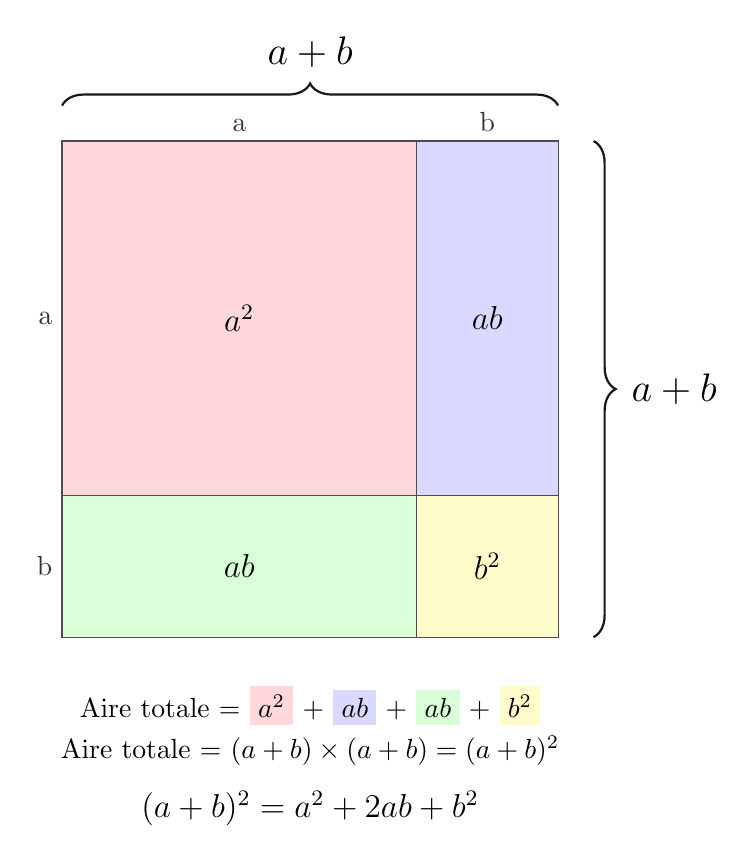
\begin{tikzpicture}[scale=1.5,font=\bfseries\large,quad/.style={draw=black!70,thin},label_side/.style={font=\normalfont\normalsize,color=black!80}]
			\def\la{3.0} \def\lb{1.2} \draw[quad, fill=red!15] (0,\lb) rectangle (\la, {\la+\lb}) node[pos=0.5] {$a^2$};
			\draw[quad, fill=blue!15] (\la,\lb) rectangle ({\la+\lb}, {\la+\lb}) node[pos=0.5] {$ab$};
			\draw[quad, fill=green!15] (0,0) rectangle (\la,\lb) node[pos=0.5] {$ab$};
			\draw[quad, fill=yellow!20] (\la,0) rectangle ({\la+\lb},\lb) node[pos=0.5] {$b^2$};
			\node[label_side, above] at ({\la/2}, {\la+\lb}) {a};
			\node[label_side, above] at ({\la+\lb/2}, {\la+\lb}) {b};
			\node[label_side, left] at (0, {\lb+\la/2}) {a};
			\node[label_side, left] at (0, {\lb/2}) {b};
			\draw[decorate, decoration={brace, amplitude=8pt}, thick, draw=black!90] (0, {\la+\lb+0.3}) -- ({\la+\lb}, {\la+\lb+0.3}) node[midway, above=10pt, font=\bfseries\Large, color=black] {$a + b$};
			\draw[decorate, decoration={brace, amplitude=8pt, mirror}, thick, draw=black!90] ({\la+\lb+0.3}, 0) -- ({\la+\lb+0.3}, {\la+\lb}) node[midway, right=10pt, font=\bfseries\Large, color=black] {$a + b$};
			\node[anchor=north, align=center, font=\normalfont\normalsize, yshift=-0.5cm] at ({(\la+\lb)/2}, 0) { Aire totale = \colorbox{red!15}{$a^2$} + \colorbox{blue!15}{$ab$} + \colorbox{green!15}{$ab$} + \colorbox{yellow!20}{$b^2$} \\[1mm] Aire totale = $(a + b) \times (a + b) = (a + b)^2$\\[3mm] \large $\Rarr (a + b)^2 = a^2 + 2ab + b^2$ };
		\end{tikzpicture}
	\end{center}
\end{rem}

\newpage
\section{Exercices}
 {\small
  \begin{multicols}{2}
	  \begin{exo}[Développement]
	Développer et réduire les expressions suivantes:
	\vspace*{-2mm}
	\begin{multicols}{2}
		\begin{enumerate}[label=\alph*)]
			\item $3(x + 2) - 4(2 - 2x)$
			\item $x(2x - 1) - 3(5 - x)$
			\item $(3x + 1)x - 3(x - 2)$
			\item $3(x - 5) - 2x(1 - 2x)$
		\end{enumerate}
	\end{multicols}
\end{exo}

	  \begin{exo}[Développement]
	Développer et réduire les expressions suivantes:
	\begin{enumerate}[label=\alph*)]
		\item $(2x + 1)(3 - 2x)$
		\item $(x - 3)(-x - 1)$
		\item $(3x + 2)(5 - 2x)$
		\item $(x - 1)(3x^{2} - 2)$
		\item $(3 - x)(2x + 1) + 2(x + 2)$
		\item $(x - 1)(2x - 1) - 3(3 + 2x)$
	\end{enumerate}
\end{exo}

	  \begin{exo}[Factorisation]
	Factoriser et réduire les expressions suivantes :
	\vspace*{-2mm}
	\begin{multicols}{2}
		\begin{enumerate}[label=\alph*)]
			\item $3x + 6$
			\item $16x - 4$
			\item $3x + 9$
			\item $4x + 6$
			\item $x^{2} + 3x$
			\item $7x + 7x^{2}$
			\item $8x^{2} + 6x$
			\item $6x + 15x^{2}$
		\end{enumerate}
	\end{multicols}
\end{exo}

	  \begin{exo}[Factorisation]
	Factoriser et réduire les expressions suivantes :
	\begin{enumerate}[label=\alph*)]
		\item $x(3x + 2) + x(5 - x)$
		\item $4(5x + 2) + 2x(5x + 2)$
		\item $(3x + 2)2x + 2x(2 - x)$
		\item $(1 - 3x)(2 + x) + (1 - 3x)(5 - 2x)$
		\item $(2x + 3)(4x + 3) - (2x + 3)(x - 1)$
		\item $(x + 5)(4 - x) - (4 - x)$
		\item $(x + 1)^{2} + (x + 1)(2x - 3)$
	\end{enumerate}
\end{exo}

	  \begin{exo}[Association d'expressions algébriques]
	Relier chaque expression de la première colonne avec sa forme développée dans la deuxième colonne.
	\begin{tabular}{p{3.5cm} @{\hspace{10mm}} p{3cm}}
		\vspace*{-2mm}
		\begin{enumerate}[label=\arabic*)]
			\item $(x + 7)^2$
			\item $(x + \sqrt{7})^2$
			\item $(x - 7)(x + 7)$
			\item $(x^2 + 7)(x^2 - 7)$
			\item $(x - 7)^2$
		\end{enumerate}
		 &
		\vspace*{-2mm}
		\begin{enumerate}[label=\alph*)]
			\item $x^2 - 14x + 49$
			\item $x^2 + 49$
			\item $x^2 + 14x + 49$
			\item $x^2 + 7x + 49$
			\item $x^2 + 2\sqrt{7}x + 7$
			\item $x^4 - 49$
			\item $x^2 - 49$
		\end{enumerate}
		\\
	\end{tabular}
\end{exo}

	  \vfill~\columnbreak
	  \begin{exo}
	À l'aide de l'identité remarquable donnée, développer les expressions algébriques suivantes.

	\def\arraystretch{1.5}
	\begin{tabular}{m{3.5cm}|m{3.5cm}}
		$(a + b)^2 = a^2 + 2ab + b^2$ & $(a - b)^2 = a^2 - 2ab + b^2$ \\ \hline
		\begin{enumerate}[label=\alph*)]
			\item $(x + 3)^2$
			\item $(2x + 8)^2$
			\item $(4 + 3x)^2$
			\item $\pa{\dfrac{1}{3} + y}^2$
		\end{enumerate}
		                              &
		\begin{enumerate}[label=\alph*)]
			\item $(x - 9)^2$
			\item $(3x - 4)^2$
			\item $(2 - 5x)^2$
			\item $(2y - \sqrt{3})^2$
		\end{enumerate}
	\end{tabular}
	\begin{center}
		\begin{tabular}{m{3.8cm}}
			$(a + b)(a - b) = a^2 - b^2$ \\ \hline
			\begin{enumerate}[label=\alph*)]
				\item $(x + 14)(x - 14)$
				\item $(7x + 9)(9 - 7x)$
				\item $\left( \dfrac{2}{3} + \dfrac{x}{4} \right)\left( \dfrac{2}{3} - \dfrac{x}{4} \right)$
				\item $\left( z + \dfrac{7}{4} \right)\left( z - \dfrac{35}{20} \right)$
			\end{enumerate}
		\end{tabular}
	\end{center}
\end{exo}

	  \begin{exo}
	À l'aide de l'identité remarquable donnée, factoriser les expressions algébriques suivantes.

	\def\arraystretch{1.5}
	\begin{tabular}{m{3.5cm}|m{3.5cm}}
		$a^2 + 2ab + b^2 = (a + b)^2$ & $a^2 - 2ab + b^2 = (a - b)^2$ \\ \hline
		\begin{enumerate}[label=\alph*)]
			\item $x^2 + 10x + 25$
			\item $9x^2 + 6x + 1$
			\item $2y + 1 + y^2$
			\item $4x^2 + 20x + 25$
		\end{enumerate}
		                              &
		\begin{enumerate}[label=\alph*)]
			\item $x^2 - 8x + 16$
			\item $9x^2 - 6x + 1$
			\item $z^2 - z + \dfrac{1}{4}$
			\item $25 + 25x^2 - 50x$
		\end{enumerate}
	\end{tabular}

	\begin{center}
		\begin{tabular}{m{3.8cm}}
			$a^2 - b^2 = (a + b)(a - b)$ \\ \hline
			\begin{enumerate}[label=\alph*)]
				\item $a^2 - 144$
				\item $9x^2 - 16$
				\item $\dfrac{x^2}{4} - \dfrac{4}{9}$
				\item $x^2 - 7$
			\end{enumerate}
		\end{tabular}
	\end{center}
\end{exo}

	  \begin{exo}
	À l'aide de l'identité remarquable la plus adaptée, développer les expressions algébriques suivantes.
	\vspace*{-2mm}
	\begin{multicols}{2}
		\begin{enumerate}[label=\alph*)]
			\item $(x + 11)^2$
			\item $(3x - 7)^2$
			\item $\left( x - \dfrac{2}{3} \right)\left( x + \dfrac{2}{3} \right)$
			\item $(5x - 9)(5x + 9)$
			\item $(2x - 1,5)^2$
			\item $(x + \sqrt{2})^2$
		\end{enumerate}
	\end{multicols}
\end{exo}

	  \begin{exo}
	À l'aide de l'identité remarquable la plus adaptée, factoriser, pour tout nombre réel $x$, les expressions algébriques suivantes.
	\vspace*{-2mm}
	\begin{multicols}{2}
		\begin{enumerate}[label=\alph*)]
			\item $x^2 + 14x + 49$
			\item $9x^2 - 30x + 25$
			\item $x^2 - \dfrac{16}{81}$
			\item $16x^2 - 4900$
			\item $6,25 + x^2 - 5x$
			\item $x^2 + \sqrt{2}x + \dfrac{1}{2}$
		\end{enumerate}
	\end{multicols}
\end{exo}

	  \vfill~\columnbreak
	  \begin{exo}
	Dans un plan, on considère une unité de longueur donnée. Soient les deux figures suivantes :

	\begin{itemize}
		\item Un rectangle dont les côtés mesurent $\pa{x - 1}$ et $\pa{x + 1}$
		\item Un carré dont le côté mesure $x$ et dans lequel on a enlevé un carré de $1$ de côté.
	\end{itemize}

	\begin{center}
		\begin{tikzpicture}[scale=0.7,>=Stealth]
			\draw[very thick] (0,0) rectangle (4,2.5);
			\draw[<->, thick] (-0.3,0) -- (-0.3,2.5) node[midway, above, sloped] {$x - 1$};
			\draw[<->, thick] (0,-0.3) -- (4,-0.3) node[midway, below] {$x + 1$};
			\begin{scope}[shift={(5.5,0)}]
				\draw[very thick] (0,0) -- (4,0) -- (4,3.5) -- (1,3.5) -- (1,2.5) -- (0,2.5) -- cycle;
				\draw[<->, thick] (0,2.7) -- (1,2.7) node[midway, above] {$1$};
				\draw[<->, thick] (0,-0.3) -- (4,-0.3) node[midway, below] {$x$};
			\end{scope}
		\end{tikzpicture}
	\end{center}

	\begin{enumerate}
		\item À quel plus grand intervalle $x$ peut-il appartenir ?
		\item À l'aide d'une calculatrice, calculer l'aire de chacune de ces figures pour différentes valeurs de $x$.
		\item Que peut-on conjecturer ?
		\item Montrer que, pour tout $x > 1$, ces deux figures ont la même aire.
	\end{enumerate}
\end{exo}

	  \begin{exo}
	Dans cet exercice, on cherche à trouver une méthode pour calculer facilement $99^2$.

	\begin{enumerate}
		\item Compléter : \cmath{99^2 = (100 - \ldots)^2 = 100^2 - 2 \times \ldots \times \ldots + 1^2 = \ldots}
		\item En remarquant que $999 = 1000 - 1$ et avec une méthode similaire, calculer $999^2$.
		\item Avec une méthode similaire, calculer $1001^2$ et $95 \times 105$.
	\end{enumerate}
\end{exo}

	  \begin{exo}
	On considère l'expression littérale $A(x) = x^2 + 8x + 15$ définie pour tout réel $x$.
	\begin{enumerate}
		\item Montrer que $A(x) = (x + 4)^2 - 1$.
		\item Montrer que $A(x) = (x + 3)(x + 5)$.
		\item En choisissant la forme de $A(x)$ la plus adaptée à un calcul mental, calculer $A(0)$, $A(-3)$, $A(-4)$ et $A(-5)$.
	\end{enumerate}
\end{exo}

	  \begin{exo}
	On considère l'expression suivante définie pour tout $x$ : \cmath{B(x) = (4x + 5)^2 - (4x + 5)(7 - x)}

	\begin{enumerate}
		\item Pour tout $x$, développer et réduire $B(x)$.
		\item Pour tout $x$, factoriser $B(x)$ à l'aide d'un facteur commun.
		\item En déduire la résolution dans $\mathbb{R}$ de \cmath{20x^2 + 17x - 10 = 0}
	\end{enumerate}
\end{exo}

	  \vfill~\columnbreak
	  \begin{exo}[Des cubes ...]
	Cette figure montre la décomposition en plusieurs solides d'un cube d'arête $a + b$ où $a$ et $b$ sont des nombres réels positifs.

	\begin{center}
		\definecolor{cubevert}{RGB}{160,200,30}
		\definecolor{cubeorange}{RGB}{250,185,40}
		\definecolor{cubebleu}{RGB}{50,170,200}
		\definecolor{cuberouge}{RGB}{225,85,35}
		\newcommand{\boite}[7]{%
			{\pgfmathsetmacro{\xb}{#1+#4}%
					\pgfmathsetmacro{\yb}{#2+#5}%
					\pgfmathsetmacro{\zb}{#3+#6}%
					\filldraw[fill=#7!70!white, draw=white, line join=round, line width=0.4pt]
					(#1,#2,\zb) -- (\xb,#2,\zb) -- (\xb,\yb,\zb) -- (#1,\yb,\zb) -- cycle;
					\filldraw[fill=#7, draw=white, line join=round, line width=0.4pt]
					(\xb,#2,#3) -- (\xb,\yb,#3) -- (\xb,\yb,\zb) -- (\xb,#2,\zb) -- cycle;
					\filldraw[fill=#7!75!black, draw=white, line join=round, line width=0.4pt]
					(#1,\yb,#3) -- (\xb,\yb,#3) -- (\xb,\yb,\zb) -- (#1,\yb,\zb) -- cycle;}%
		}

		\begin{tikzpicture}[scale=1.1, x={(-0.21cm,-0.12cm)}, y={(0.21cm,-0.12cm)}, z={(0cm,0.24cm)}, font=\small]
			\begin{scope}
				\boite{0}{0}{0}{2}{2}{2}{cubevert}
				\node[right=-1mm] at (0,2,1) {$a$};
			\end{scope}
			\begin{scope}[xshift=1.9cm]
				\boite{0}{0}{0}{2}{2}{2}{cubevert}
				\boite{2}{0}{0}{1}{2}{2}{cubeorange}
				\boite{0}{0}{2}{2}{2}{1}{cubeorange}
				\node[right=-3mm] at (0,3,3.2) {$b$};
				\node[right=-3mm] at (0,3,1.6) {$a$};
			\end{scope}
			\begin{scope}[xshift=3.8cm]
				\boite{2}{0}{0}{1}{2}{2}{cubeorange}
				\boite{0}{2}{0}{2}{1}{2}{cubeorange}
				\boite{0}{0}{2}{2}{2}{1}{cubeorange}
				\node[right=-3mm] at (0,3,3.2) {$b$};
				\node[right=1mm] at (0,2.3,0.6) {$a$};
			\end{scope}
			\begin{scope}[xshift=0.8cm, yshift=-1.5cm]
				\boite{2}{0}{0}{1}{2}{2}{cubeorange}
				\boite{0}{2}{0}{2}{1}{2}{cubeorange}
				\boite{0}{0}{2}{2}{2}{1}{cubeorange}
				\boite{2}{2}{0}{1}{1}{2}{cubebleu}
				\boite{2}{0}{2}{1}{2}{1}{cubebleu}
				\boite{0}{2}{2}{2}{1}{1}{cubebleu}
				\node[right=-1mm] at (0,3,2.5) {$b$};
				\node[right=-1mm] at (0,3,1)   {$a$};
			\end{scope}
			\begin{scope}[xshift=2.7cm,yshift=-1.5cm]
				\boite{2}{0}{0}{1}{2}{2}{cubeorange}
				\boite{0}{2}{0}{2}{1}{2}{cubeorange}
				\boite{0}{0}{2}{2}{2}{1}{cubeorange}
				\boite{2}{2}{0}{1}{1}{2}{cubebleu}
				\boite{2}{0}{2}{1}{2}{1}{cubebleu}
				\boite{0}{2}{2}{2}{1}{1}{cubebleu}
				\boite{2}{2}{2}{1}{1}{1}{cuberouge}
				\node[right=-1mm] at (0,3,2.5) {$b$};
				\node[right=-1mm] at (0,3,1)   {$a$};
			\end{scope}
		\end{tikzpicture}
	\end{center}

	\begin{enumerate}
		\item Pour chaque couleur de solide (vert, jaune, bleu et rouge) :
		      \begin{enumerate}
			      \item Déterminer le nombre de solides.
			      \item Déterminer le volume d'un solide en fonction de $a$ et $b$.
		      \end{enumerate}
		\item Montrer que $(a + b)^3 = a^3 + 3a^2b + 3ab^2 + b^3$.
		\item Cette égalité est-elle démontrée pour tous $a$ et $b$ ?
	\end{enumerate}
\end{exo}

	  \begin{exo}[... et des carrés]
	On considère le carré $ABCD$ de côtés $6\text{ cm}$ et quatre points $M$, $N$, $P$, $Q$ tels que $AM = BN = CP = DQ$

	On admet que $MNPQ$ est un carré et on note $x = BM$

	\begin{center}
		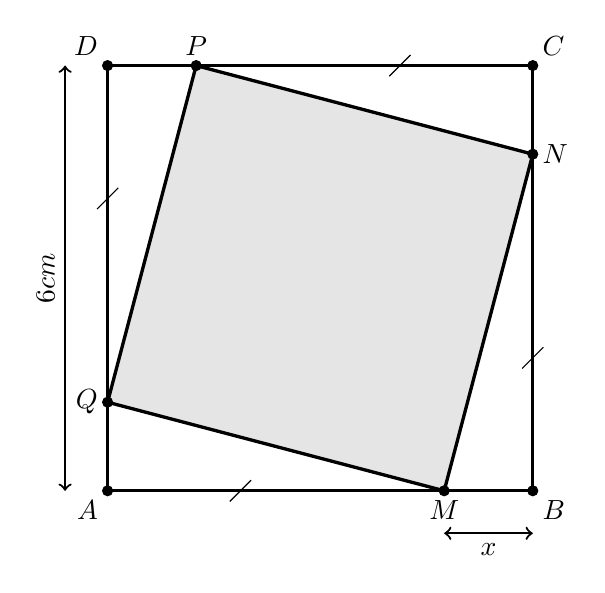
\begin{tikzpicture}[scale=0.9]
			\coordinate (A) at (0,0);
			\coordinate (B) at (6,0);
			\coordinate (C) at (6,6);
			\coordinate (D) at (0,6);
			\draw[very thick] (A) -- (B) -- (C) -- (D) -- cycle;
			\node[below left] at (A) {$A$};
			\node[below right] at (B) {$B$};
			\node[above right] at (C) {$C$};
			\node[above left] at (D) {$D$};
			\coordinate (M) at (4.75,0);
			\coordinate (N) at (6,4.75);
			\coordinate (P) at (1.25,6);
			\coordinate (Q) at (0,1.25);
			\draw[very thick, fill=black!10] (M) -- (N) -- (P) -- (Q) -- cycle;
			\node[below] at (M) {$M$};
			\node[right] at (N) {$N$};
			\node[above] at (P) {$P$};
			\node[left] at (Q) {$Q$};
			\draw[<->, thick] (-0.6,0) -- (-0.6,6) node[midway, above, sloped] {$6\text{ cm}$};
			\draw[<->, thick] (4.75,-0.6) -- (6,-0.6) node[midway, below] {$x$};
			\draw[shift={(1.875,0)}] (-0.15,-0.15) -- (0.15,0.15);
			\draw[shift={(6,1.875)}] (-0.15,-0.15) -- (0.15,0.15);
			\draw[shift={(4.125,6)}] (-0.15,-0.15) -- (0.15,0.15);
			\draw[shift={(0,4.125)}] (-0.15,-0.15) -- (0.15,0.15);
			\foreach \pt in {A,B,C,D,M,N,P,Q} { \filldraw[black] (\pt) circle (2pt); }
		\end{tikzpicture}
	\end{center}

	\begin{enumerate}
		\item Justifier que l'aire $\mathcal{A}$ du carré $MNPQ$ a pour valeur : \cmath{\mathcal{A} = 2x^2 - 12x + 36}
	\end{enumerate}

	\textbf{Aide :} $\text{Aire}(MNPQ) = \text{Aire}(ABCD) - 4 \times \text{Aire}(AMQ)$

	\begin{enumerate}[resume]
		\item \begin{enumerate}
			      \item Montrer que : \cmath{2(x - 2)(x - 4)\ =\ 2x^2 - 12x + 16}
			      \item Déterminer la ou les valeurs de $x$ afin que l'aire du carré $MNPQ$ soit égale aux $\dfrac{5}{9}$ de celle du carré $ABCD$.
		      \end{enumerate}
	\end{enumerate}
\end{exo}

	  \vfill~
  \end{multicols}
 }

\chapter{Multiples et diviseurs}

\section{Multiples et diviseurs}

\begin{definition}[Multiple et diviseur]
	Soit $a$ et $b$ deux entiers naturels.

	On dit que $a$ est un \textbf{multiple} de $b$ s'il existe un entier $k$ tel que :
	\[
		a = k \times b
	\]

	On dit alors que $b$ est un \textbf{diviseur} de $a$.
\end{definition}

\begin{exemple}
	$15$ est un multiple de $3$, car $15 = 5 \times 3$ (avec $k = 5$).
\end{exemple}

\begin{methode}[Démontrer qu'un nombre est multiple ou diviseur]
	Les affirmations suivantes sont-elles vraies ou fausses ?
	\begin{multicols}{2}
		\begin{enumerate}[label=\alph*)]
			\item $36$ est un multiple de $12$.
			\item $28$ est un multiple de $8$.
			\item $6$ est un diviseur de $54$.
			\item $7$ est un diviseur de $24$.
		\end{enumerate}
	\end{multicols}

	\begin{correction}
		\nline
		\begin{enumerate}[label=\alph*)]
			\item \textbf{VRAI :} $36$ est un multiple de $12$, car $36 = 3 \times 12$ avec $k = 3$.
			\item \textbf{FAUX :} $28$ n'est pas un multiple de $8$ car il n'existe aucun entier $k$ tel que $28 = k \times 8$.
			\item \textbf{VRAI :} $6$ est un diviseur de $54$, car $54 = 9 \times 6$ avec $k = 9$.
			\item \textbf{FAUX :} $7$ n'est pas un diviseur de $24$ car il n'existe aucun entier $k$ tel que $24 = k \times 7$.
		\end{enumerate}
	\end{correction}
\end{methode}

\begin{propriete}[Somme de multiples]
	La \textbf{somme} de deux multiples d'un entier naturel $m$ est un multiple de $m$.

	Autrement dit, si $b = k_1 \times m$ et $c = k_2 \times m$ (avec $k_1$ et $k_2$ entiers), alors :
	\[
		b + c = k \times m\qquad \text{avec}\; k\; {entier}
	\]
\end{propriete}

\begin{exemple}
	$700$ et $21$ sont des multiples de $7$, donc $721 = 700 + 21$ est aussi un multiple de $7$.
\end{exemple}

\begin{demo}[La somme de deux multiples de $m$ est un multiple de $m$]
	Soit $m$ un entier naturel. Soit $b$ et $c$ deux multiples de $m$.

	Comme $b$ est un multiple de $m$, il existe un entier $k_1$ tel que $b = m \times k_1$.

	Comme $c$ est un multiple de $m$, il existe un entier $k_2$ tel que $c = m \times k_2$.

	Alors :
	\[
		b + c = m \times k_1 + m \times k_2 = m \times (k_1 + k_2) = m \times k, \quad \text{où } k = k_1 + k_2.
	\]

	$k = k_1 + k_2$ est un entier, donc $b + c$ est de la forme $m \times k$ avec $k$ entier.

	Ainsi, $b + c$ est bien un multiple de $m$.
\end{demo}

\newpage

\begin{methode}[Résoudre un problème avec des multiples]
	Montrer que la somme de trois entiers consécutifs est toujours un multiple de $3$.

	\begin{correction}
		Soit trois entiers consécutifs notés $n$, $n + 1$ et $n + 2$, où $n$ est un entier naturel quelconque.

		Leur somme $S$ vaut :
		\[
			S = n + (n + 1) + (n + 2) = 3n + 3 = 3(n + 1).
		\]

		En posant $k = n + 1$ ($k$ est un entier), on a $S = 3k$.

		$S$ est donc bien un multiple de $3$.
	\end{correction}
\end{methode}

\section{Nombres pairs et impairs}

\begin{definition}[Parité]
	Un nombre entier est \textbf{pair} s'il est un multiple de $2$.

	Un nombre entier est \textbf{impair} s'il n'est pas pair.

	\begin{itemize}
		\item Un nombre pair s'écrit sous la forme $2k$, avec $k$ entier.
		\item Un nombre impair s'écrit sous la forme $2k + 1$, avec $k$ entier.
	\end{itemize}
\end{definition}

\begin{exemple}
	\nline
	\begin{itemize}
		\item $34$ est pair car $34 = 2 \times 17$.
		\item $57$ est impair car $57 = 2 \times 28 + 1$.
	\end{itemize}
\end{exemple}

\begin{propriete}[Règles de parité]
	\nline
	\begin{center}
		\def\arraystretch{1.4}%
		\begin{tabular}{c|c|c}%
			$+$ ou $-$ & pair   & impair \\
			\hline
			pair       & pair   & impair \\
			impair     & impair & pair   \\
		\end{tabular}
		\qquad\qquad
		\begin{tabular}{c|c|c}%
			$\times$ & pair & impair \\
			\hline
			pair     & pair & pair   \\
			impair   & pair & impair \\
		\end{tabular}
	\end{center}
\end{propriete}

\begin{demo}
	\nline
	\begin{enumerate}
		\item \textbf{Produit d'un pair et d'un impair :}

		      Soit $n$ un nombre pair et $m$ un nombre impair.

		      Il existe deux entiers $k$ et $p$ tels que $n = 2k$ et $m = 2p + 1$.

		      On calcule leur produit :
		      \[
			      n \times m = 2k \times (2p + 1) = 2 \times [k(2p + 1)]
		      \]
		      En posant $K = k(2p + 1)$, qui est un entier, on obtient $n \times m = 2K$.

		      Le produit est donc de la forme $2K$ : c'est un nombre \textbf{pair}.

		\item \textbf{Produit de deux impairs :}

		      Soit $n$ et $m$ deux nombres impairs.

		      Il existe deux entiers $k$ et $p$ tels que $n = 2k + 1$ et $m = 2p + 1$.

		      On développe leur produit :
		      \begin{align*}
			      n \times m & = (2k + 1)(2p + 1)   \\
			                 & = 4kp + 2k + 2p + 1  \\
			                 & = 2(2kp + k + p) + 1
		      \end{align*}
		      En posant $K' = 2kp + k + p$, qui est un entier, on obtient $n \times m = 2K' + 1$.

		      Le produit est donc de la forme $2K' + 1$ : c'est un nombre \textbf{impair}.
	\end{enumerate}
\end{demo}

\begin{methode}[Déterminer la parité d'un nombre]
	Quelle est la parité de $\np{5678984}^2 + 1$ ?

	\begin{correction}
		$\def\arraystretch{1.2}%
			\begin{array}{rl}%
				\np{5678984}^2 = & \np{5678984} \times \np{5678984}                 \\
				=                & \text{PAIR} \times \text{PAIR} \Rarr \text{PAIR} \\
				=                & 2k, \text{ avec } k \text{ entier.}
			\end{array}$%

		\ms

		Donc $5\,678\,984^2 + 1 = 2k + 1$, ce qui prouve que ce nombre est \textbf{impair}.
	\end{correction}
\end{methode}

\begin{propriete}[Carré d'un impair]
	Le carré d'un nombre impair est un nombre impair.
\end{propriete}

\begin{demo}[Le carré d'un impair est impair]
	Soit $a$ un nombre impair.

	Il s'écrit $a = 2k + 1$, avec $k$ entier.

	Alors :
	\[
		a^2 = \pa{2k + 1}^2 = 4k^2 + 4k + 1 = 2\pa{2k^2 + 2k} + 1 = 2k' + 1,
	\]

	\ldots avec $k' = 2k^2 + 2k$ entier (somme de produits d'entiers).

	Comme $a^2$ s'écrit sous la forme $2k' + 1$, $a^2$ est bien impair.
\end{demo}

\begin{methode}[Résoudre un problème de parité]
	Montrer que le produit de deux entiers consécutifs est toujours un nombre pair.

	\begin{correction}
		Soit deux entiers consécutifs $n$ et $n + 1$.
		\begin{itemize}
			\item \textbf{Cas 1 :} $n$ est pair.

			      Alors $n = 2k$ avec $k$ entier, et :

			      \[
				      n(n + 1) = 2k(2k + 1) = 2k_1, \quad \text{avec } k_1 = k(2k + 1) \text{ entier}.
			      \]

			      Donc $n(n + 1)$ est pair.

			\item \textbf{Cas 2 :} $n$ est impair.

			      Alors $n = 2k + 1$ avec $k$ entier, et :

			      \[
				      n(n + 1) = (2k + 1)(2k + 2) = 2(2k + 1)(k + 1) = 2k_2, \quad \text{avec } k_2 = (2k + 1)(k + 1) \text{ entier}.
			      \]

			      Donc $n(n + 1)$ est pair.
		\end{itemize}

		\textbf{Conclusion :} Dans tous les cas, le produit de deux entiers consécutifs est un nombre pair.
	\end{correction}
\end{methode}

\section{Nombres premiers}

\begin{definition}[Nombre premier]
	Un entier naturel est \textbf{premier} s'il possède exactement deux diviseurs distincts : $1$ et lui-même.
\end{definition}

\begin{exemple}[Nombres premiers]
	Les premiers nombres premiers sont : $2, 3, 5, 7, 11, 13, 17, 19, 23, \ldots$ (il y en a une infinité).

\end{exemple}

\begin{rem}
	Le nombre $1$ n'est \textbf{pas} premier car il n'a qu'un seul diviseur ($1$).
\end{rem}

\newpage

\begin{propriete}[Critère d'arrêt]
	Soit $n$ un entier naturel supérieur ou égal à $2$.

	Si $n$ n'est pas un nombre premier, alors il possède au moins un diviseur premier $p$ tel que :
	\[
		p \leqslant \sqrt{n}
	\]
\end{propriete}

\begin{demo}
	Soit $n \geqslant 2$ un entier non premier (on dit aussi composé).

	$n$ admet donc au moins deux diviseurs stricts distincts de $1$ et de lui-même.

	On peut donc écrire $n = a \times b$, où $a$ et $b$ sont deux entiers naturels vérifiant $1 < a \leqslant b < n$.

	Raisonnons par l'absurde et supposons que $a > \sqrt{n}$ et $b > \sqrt{n}$.

	En multipliant ces deux inégalités strictement positives membre à membre, on obtient :
	\[
		a \times b > \sqrt{n} \times \sqrt{n}\iff n > n
	\]

	Ce qui est absurde.

	L'hypothèse de départ est donc fausse : l'un au moins des deux facteurs est inférieur ou égal à $\sqrt{n}$.
\end{demo}
\begin{methode}[Vérifier si un nombre est premier]
	Démontrer que le nombre $97$ est premier.

	\begin{correction}
		On calcule $\sqrt{97} \approx 9{,}8$. On teste la divisibilité de $97$ par tous les \textbf{nombres premiers} inférieurs ou égaux à $\sqrt{97}$, c'est-à-dire : $2$, $3$, $5$ et $7$.

		\begin{itemize}
			\item \textbf{2 :} Non - $97$ est impair (il se termine par $7$).
			\item \textbf{3 :} Non - La somme de ses chiffres vaut $9 + 7 = 16$, qui n'est pas un multiple de $3$.
			\item \textbf{5 :} Non - $97$ ne se termine ni par $0$ ni par $5$.
			\item \textbf{7 :} Non - $97 = 7 \times 13 + 6$ (la division euclidienne donne un reste non nul).
		\end{itemize}

		Comme $97$ n'est divisible par aucun nombre premier inférieur ou égal à $\sqrt{97}$, le nombre $97$ est un \textbf{nombre premier}.
	\end{correction}
\end{methode}

\begin{propriete}[Décomposition en facteurs premiers]
	Tout entier $n \geqslant 2$ se décompose de manière unique (à l'ordre des facteurs près) sous la forme :
	\[
		n = p_1^{a_1} \times p_2^{a_2} \times \cdots \times p_k^{a_k}
	\]

	\ldots où $p_1, p_2, \ldots, p_k$ sont des nombres premiers distincts et $a_1, a_2, \ldots, a_k$ sont des entiers naturels non nuls.
\end{propriete}

\begin{exemple}[Décomposition]
	\[
		\def\arraystretch{1.2}%
		\begin{array}{r|l}%
			300 & 2 \\
			150 & 2 \\
			75  & 3 \\
			25  & 5 \\
			5   & 5 \\
			1   &
		\end{array}\qquad\Rarr\qquad 300 = 2 \times 2 \times 3 \times 5 \times 5 = 2^2 \times 3 \times 5^2
	\]
\end{exemple}

\newpage

\begin{definition}[Fraction irréductible]
	Une fraction est dite \textbf{irréductible} lorsque son numérateur et son dénominateur n'ont aucun diviseur commun autre que $1$.
\end{definition}

\begin{methode}[Rendre une fraction irréductible]
	Rendre irréductible la fraction $\dfrac{60}{126}$.

	\begin{correction}
		On décompose le numérateur et le dénominateur en produit de facteurs premiers :
		\[
			\def\arraystretch{1.2}%
			\begin{array}{r|l}%
				60 & 2 \\
				30 & 2 \\
				15 & 3 \\
				5  & 5 \\
				1  &
			\end{array}%
			\quad \Rarr \quad 60 = 2 \times 2 \times 3 \times 5 \qquad\qquad \def\arraystretch{1.2}%
			\begin{array}{r|l}%
				126 & 2 \\
				63  & 3 \\
				21  & 3 \\
				7   & 7 \\
				1   &
			\end{array}%
			\quad \Rarr \quad 126 = 2 \times 3 \times 3 \times 7
		\]

		\ms

		On simplifie les facteurs communs ($2$ et $3$) :
		\[
			\frac{60}{126} = \frac{\cancel{2} \times 2 \times \cancel{3} \times 5}{\cancel{2} \times \cancel{3} \times 3 \times 7} = \frac{2 \times 5}{3 \times 7} = \frac{10}{21}
		\]

		$10$ et $21$ n'ont aucun diviseur commun autre que $1$, donc $\dfrac{10}{21}$ est la forme irréductible.
	\end{correction}
\end{methode}

\begin{rem}[Crible d'Ératosthène]
	Le crible d'Ératosthène est un procédé algorithmique permettant de trouver tous les nombres premiers inférieurs ou égaux à une valeur donnée $N$ (ici $N = 100$).

	\begin{center}
		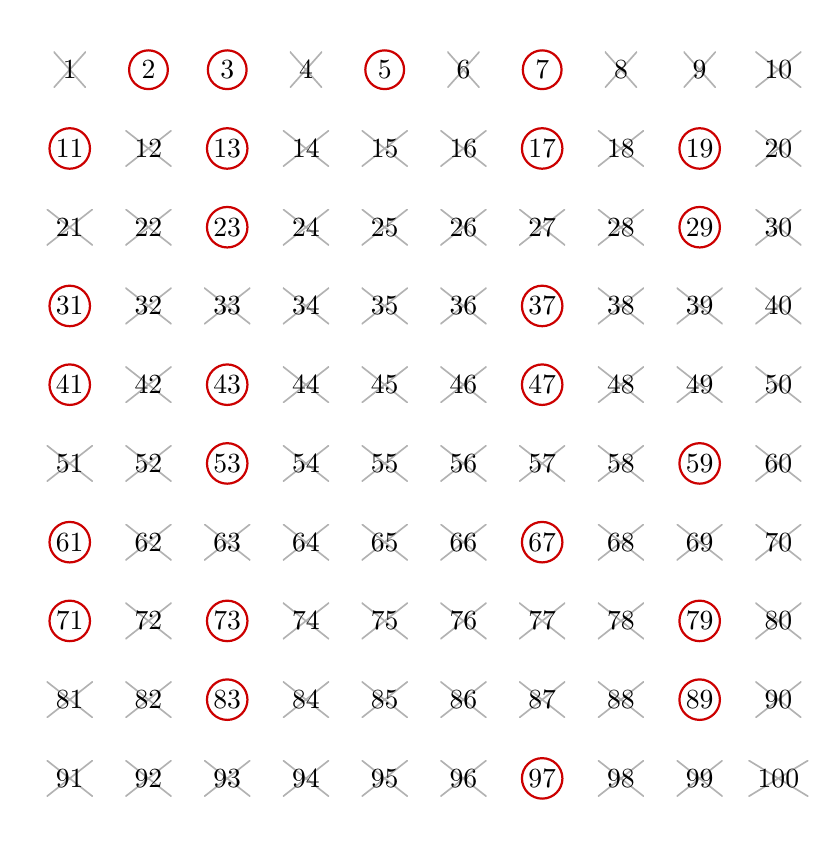
\begin{tikzpicture}[prime/.style={draw=red!80!black, thick, circle, fill=white, inner sep=1pt, minimum size=14pt},crossed/.style={ path picture={ \draw[gray!60, line width=0.6pt] (path picture bounding box.south west) -- (path picture bounding box.north east) (path picture bounding box.south east) -- (path picture bounding box.north west); } } ]
			\foreach \n in {1,...,100} { \pgfmathtruncatemacro{\r}{int((\n-1)/10)} \pgfmathtruncatemacro{\c}{\n - \r*10} \node[crossed] at (\c, 10-\r) {\n}; }
			\foreach \p in {2,3,5,7,11,13,17,19,23,29,31,37,41,43,47,53,59,61,67,71,73,79,83,89,97} { \pgfmathtruncatemacro{\r}{int((\p-1)/10)} \pgfmathtruncatemacro{\c}{\p - \r*10} \filldraw[white] (\c, 10-\r) circle (15pt); \node[prime] at (\c, 10-\r) {\p}; }
		\end{tikzpicture}
	\end{center}
\end{rem}

\newpage
\section{Exercices}
 {\small
  \begin{multicols}{2}
	  \begin{exo}{}
	Parmi les nombres suivants, donner les multiples de $5$, les multiples de $17$ et les multiples de $6$. Justifier.
	\vspace*{-2mm}\begin{multicols}{4}
		\begin{enumerate}
			\item $10$
			\item $85$
			\item $510$
			\item $28$
			\item $34$
			\item $60$
			\item $72$
			\item $97$
		\end{enumerate}
	\end{multicols}
\end{exo}

	  \begin{exo}{}
	On considère les nombres $a = 35$ et $b = 25$.
	\begin{enumerate}
		\item Donner un multiple de $a$ et un multiple de $b$.
		\item Donner un nombre qui est multiple simultanément de $a$ et $b$, c'est un multiple commun à $a$ et à $b$.
		\item Parmi tous les nombres strictement positifs qui sont multiples simultanément de $a$ et $b$, quel est le plus petit ?
	\end{enumerate}
\end{exo}

	  \begin{exo}{}
	On considère les nombres $a = 24$ et $b = 18$.
	\begin{enumerate}
		\item Donner un multiple de $a$ et un multiple de $b$.
		\item Donner un nombre qui est multiple simultanément de $a$ et $b$.
		\item Parmi tous les nombres strictement positifs qui sont multiples simultanément de $a$ et $b$, quel est le plus petit ?
	\end{enumerate}
\end{exo}

	  \begin{exo}{}
	Dans chaque cas, donner tous les diviseurs de chacun des deux nombres, puis déterminer les diviseurs communs. Parmi ceux-là, déduire le plus grand diviseur commun aux deux nombres.
	\vspace*{-2mm}\begin{multicols}{2}
		\begin{enumerate}
			\item $15$ et $35$
			\item $60$ et $40$
			\item $45$ et $64$
			\item $270$ et $180$
		\end{enumerate}
	\end{multicols}
\end{exo}

	  \begin{exo}{}
	Dans chaque cas, chercher le plus grand diviseur commun au numérateur et au dénominateur, puis mettre la fraction sous forme irréductible.
	\vspace*{-2mm} \begin{multicols}{4}
		\begin{enumerate}
			\item $\dfrac{45}{20}$
			\item $\dfrac{63}{42}$
			\item $\dfrac{121}{56}$
			\item $\dfrac{51}{85}$
		\end{enumerate}
	\end{multicols}\vspace*{-2mm}
\end{exo}

	  \begin{exo}{}
	Trouver tous les diviseurs premiers des nombres suivants.
	\vspace*{-2mm}\begin{multicols}{4}
		\begin{enumerate}
			\item $21$
			\item $56$
			\item $256$
			\item $301$
		\end{enumerate}
	\end{multicols}
\end{exo}

	  \begin{exo}{}
	\nline
	\begin{enumerate}
		\item Déterminer la liste de tous les nombres premiers compris entre $1$ et $30$.
		\item Parmi ces nombres, quels sont ceux qui sont pairs ?
		\item Existe-t-il d'autres nombres premiers pairs ? Justifier.
	\end{enumerate}
\end{exo}

	  \vfill~\columnbreak
	  \begin{exo}{}
	La conjecture de Goldbach affirme que :

	\og{} Tout nombre pair supérieur ou égal à $4$ est la somme de deux nombres premiers \fg{}.

	\begin{enumerate}
		\item Vérifier cette conjecture pour tous les nombres pairs de l'intervalle $\intff{10}{20}$.
		\item Trouver tous les nombres premiers $p$ et $p'$ tels que $100 = p + p'$.
	\end{enumerate}
\end{exo}

	  \begin{exo}{}
	Soient $a$ et $a'$ deux nombres impairs.
	\begin{enumerate}
		\item Montrer que $a^2 + (a')^2$ est un nombre pair.
	\end{enumerate}
\end{exo}

	  \begin{exo}{}
	\begin{enumerate}
		\item Démontrer la proposition suivante : \og{} Un entier est pair si, et seulement si, son carré est pair. \fg{}
	\end{enumerate}
\end{exo}

	  \begin{exo}{}
	Soit $a$ un nombre impair.
	\begin{enumerate}
		\item Démontrer que $a^3$ est un nombre impair.
	\end{enumerate}
\end{exo}

	  \begin{exo}{}
	Une crèche dispose de $60$ dalles carrées en mousse. Elle souhaite les placer de manière à former un rectangle.
	\begin{enumerate}
		\item Quelles sont les dimensions possibles de ce rectangle ?
		\item Quel est celui qui a le plus grand périmètre ?
	\end{enumerate}
\end{exo}

	  \begin{exo}{}
	Lors d'un tournoi de pétanque, il y a $80$ hommes et $60$ femmes inscrits.

	L'organisation veut constituer un maximum d'équipes mixtes contenant toutes le même nombre d'hommes et le même nombre de femmes.

	\begin{enumerate}
		\item Combien d'équipes peuvent être constituées ?
	\end{enumerate}
\end{exo}

	  \begin{exo}{}
	Un pâtissier a préparé $112$ macarons au chocolat et $96$ macarons à la framboise.

	Il souhaite répartir la totalité de ces macarons dans des boîtes identiques pour les vendre.
	\begin{enumerate}
		\item Peut-il faire $6$ boîtes ? Justifier.
		\item Quel est le nombre maximal de boîtes qu'il peut réaliser ?
		\item Quelle sera alors la composition de chaque boîte ?
	\end{enumerate}
\end{exo}

	  \vfill~
  \end{multicols}
 }

\chapter{Ensembles de nombres et intervalles}

\section{Ensembles de nombres}

\subsection{L'ensemble des entiers naturels $\N$}

\begin{df}
	\nline
	\begin{wrapstuff}[r,width=3cm]
		\begin{center}
			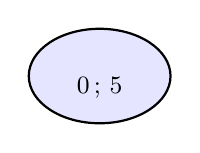
\begin{tikzpicture}[scale=0.75]
				\draw[thick, fill=blue!10] (0,0) ellipse (1.2cm and 0.8cm);
				\node at (0,0.3) {\textbf{$\N$}};
				\node[font=\small] at (0,-0.2) {$0 \,;\, 5$};
			\end{tikzpicture}
		\end{center}
	\end{wrapstuff}

	L'\textbf{ensemble des entiers naturels}, noté $\N$, est l'ensemble des entiers positifs ou nuls.
	\[
		\N = \{0\,;\, 1\,;\, 2\,;\, 3\,;\, 4\,;\, \dots\}
	\]
\end{df}

\begin{ex}
	$5 \in \N$ \quad et \quad $0 \in \N$.
\end{ex}

\subsection{L'ensemble des entiers relatifs $\Z$}

\begin{df}
	\nline
	\begin{wrapstuff}[r,width=4cm]
		\begin{center}
			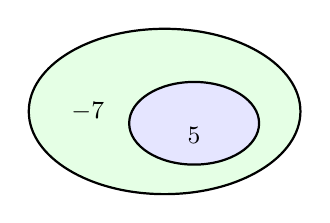
\begin{tikzpicture}[scale=0.75]
				\draw[thick, fill=green!10] (0,0) ellipse (2.3cm and 1.4cm);
				\node at (0,1) {\textbf{$\Z$}};
				\node[font=\small] at (-1.3,0) {$-7$};
				\draw[thick, fill=blue!10] (0.5,-0.2) ellipse (1.1cm and 0.7cm);
				\node at (0.5,0.05) {\textbf{$\N$}};
				\node[font=\small] at (0.5,-0.4) {$5$};
			\end{tikzpicture}
			\vspace*{-10mm}
		\end{center}
	\end{wrapstuff}
	L'\textbf{ensemble des entiers relatifs}, noté $\Z$, est l'ensemble des entiers positifs, négatifs ou nuls.
	\[
		\Z = \{\dots\,;\, - 3\,;\, - 2\,;\, - 1\,;\, 0\,;\, 1\,;\, 2\,;\, 3\,;\, \dots\}
	\]
\end{df}

\begin{ex}
	$-7 \in \Z$ \quad et \quad $5 \in \Z$ (tout entier naturel est aussi un entier relatif).
\end{ex}

\subsection{L'ensemble des nombres décimaux $\D$}

\begin{df}
	\nline
	\begin{wrapstuff}[r,width=5cm]
		\begin{center}
			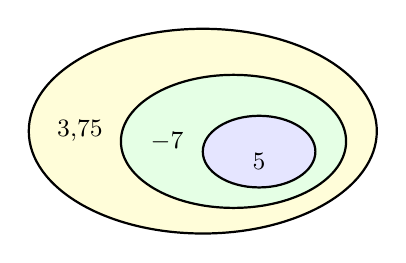
\begin{tikzpicture}[scale=0.65]
				\draw[thick, fill=yellow!15] (0,0) ellipse (3.4cm and 2cm);
				\node at (0,1.5) {\textbf{$\D$}};
				\node[font=\small] at (-2.4,0) {$3{,}75$};
				\draw[thick, fill=green!10] (0.6,-0.2) ellipse (2.2cm and 1.3cm);
				\node at (0.6,0.7) {\textbf{$\Z$}};
				\node[font=\small] at (-0.7,-0.2) {$-7$};
				\draw[thick, fill=blue!10] (1.1,-0.4) ellipse (1.1cm and 0.7cm);
				\node at (1.1,-0.15) {\textbf{$\N$}};
				\node[font=\small] at (1.1,-0.6) {$5$};
			\end{tikzpicture}
			\vspace*{-20mm}
		\end{center}
	\end{wrapstuff}

	L'\textbf{ensemble des nombres décimaux}, noté $\D$, est l'ensemble des nombres qui peuvent s'écrire sous la forme $\frac{a}{10^n}$, où $a \in \Z$ et $n \in \N$.

\end{df}

\begin{remarque}
	Un nombre décimal possède un \textbf{nombre fini de chiffres après la virgule}.
\end{remarque}

\begin{ex}
	$3{,}75 \in \D$ \quad car \quad $3{,}75 = \dfrac{375}{10^2}$
\end{ex}

\subsection{L'ensemble des nombres rationnels $\Q$}

\begin{df}
	\nline
	\begin{wrapstuff}[r,width=5.7cm]
		\begin{center}
			\begin{tikzpicture}[scale=0.55]
				\draw[thick, fill=orange!15] (0,0) ellipse (4.5cm and 2.6cm);
				\node at (0,2.1) {\textbf{$\Q$}};
				\node[font=\small] at (-3.2,0) {$\dfrac{1}{3}$};
				\draw[thick, fill=yellow!15] (0.7,-0.2) ellipse (3.3cm and 1.9cm);
				\node at (0.7,1.3) {\textbf{$\D$}};
				\node[font=\small] at (-1.7,-0.2) {$3{,}75$};
				\draw[thick, fill=green!10] (1.3,-0.4) ellipse (2.2cm and 1.2cm);
				\node at (1.3,0.4) {\textbf{$\Z$}};
				\node[font=\small] at (0,-0.4) {$-7$};
				\draw[thick, fill=blue!10] (1.8,-0.6) ellipse (1cm and 0.6cm);
				\node at (1.8,-0.35) {\textbf{$\N$}};
				\node[font=\small] at (1.8,-0.87) {$5$};
			\end{tikzpicture}
		\end{center}
		\vspace*{-10mm}
	\end{wrapstuff}

	L'\textbf{ensemble des nombres rationnels}, noté $\Q$, est l'ensemble des nombres qui peuvent s'écrire sous la forme d'une fraction $\frac{a}{b}$, avec $a \in \Z$ et $b \in \Z^*$ ($b \neq 0$).

	Son écriture décimale possède une \textbf{suite de chiffres qui se répète périodiquement} après la virgule.
\end{df}

\begin{ex}
	$\dfrac{1}{3} \in \Q$ \quad car \quad $\dfrac{1}{3} = 0{,}3333\dots$ (non décimal, mais rationnel ... voir démonstration ci-dessous).
\end{ex}

\begin{demo}[$\frac{1}{3}$ n'est pas un nombre décimal]
	On effectue un raisonnement par l'absurde.

	Supposons que $\tfrac{1}{3}$ soit un nombre décimal.

	Alors, par définition, il pourrait s'écrire sous la forme :

	\[
		\frac{1}{3} = \frac{a}{10^n} \quad \text{avec } a \in \Z \text{ et } n \in \N
	\]

	En effectuant le produit en croix, on obtient :

	\[
		3 \times a = 10^n \times 1 \implies 3a = 10^n
	\]

	Cela signifie que $10^n$ doit être un multiple de $3$.

	Or, un nombre est divisible par $3$ si la somme de ses chiffres est un multiple de $3$.

	La somme des chiffres de $10^n$ (qui s'écrit $1$ suivi de $n$ zéro(s)) est égale à $1 + 0 + \dots + 0 = 1$.

	Puisque $1$ n'est pas divisible par $3$, $10^n$ n'est jamais un multiple de $3$.

	Nous obtenons une \textbf{contradiction}.

	L'hypothèse de départ est donc fausse : $\frac{1}{3}$ n'est pas un nombre décimal $\pa{\frac{1}{3} \notin \D}$.
\end{demo}

\subsection{L'ensemble des nombres réels $\R$}

\begin{df}
	L'\textbf{ensemble des nombres réels}, noté $\R$, est l'ensemble de tous les nombres connus en Seconde (représentés par tous les points de la droite graduée).

	Il contient les nombres rationnels ainsi que les \textbf{nombres irrationnels}, qui ne peuvent pas s'écrire sous forme de fraction.
\end{df}

\begin{ex}
	$\sqrt{2} \in \R$ \quad et \quad $\pi \in \R$ \quad (ce sont des nombres irrationnels).
\end{ex}

\begin{demo}[$\sqrt{2}$ n'est pas un nombre rationnel]

	On effectue à nouveau un raisonnement par l'absurde.

	Supposons que $\sqrt{2}$ soit un nombre rationnel.

	Alors $\sqrt{2}$ s'écrit sous la forme d'une fraction irréductible :

	\[
		\sqrt{2} = \frac{a}{b} \quad \text{avec } a \in \N^*, b \in \N^*
	\]

	En élevant au carré des deux côtés :

	\[
		2 = \frac{a^2}{b^2} \implies a^2 = 2b^2
	\]

	Comme $a^2$ s'écrit sous la forme $2k$ (avec $k = b^2$), $a^2$ est un nombre \textbf{pair}.

	Or, le carré d'un nombre impair est impair. Ainsi, comme $a^2$ est pair, \textbf{$a$ est nécessairement pair}.

	Puisque $a$ est pair, il existe un entier $k \in \N^*$ tel que $a = 2k$.

	En remplaçant dans l'égalité $a^2 = 2b^2$ :

	\[
		(2k)^2 = 2b^2 \implies 4k^2 = 2b^2 \implies b^2 = 2k^2
	\]

	De même, $b^2$ s'écrit $2k^2$, donc $b^2$ est pair, ce qui implique que \textbf{$b$ est aussi pair}.

	Si $a$ et $b$ sont tous les deux pairs, ils sont tous les deux divisibles par $2$.

	Cela contredit le fait que $\dfrac{a}{b}$ est irréductible.

	Nous obtenons une \textbf{contradiction}.

	L'hypothèse de départ est donc fausse : $\sqrt{2}$ n'est pas un nombre rationnel ($\sqrt{2} \notin \Q$).
\end{demo}

\begin{prop}[Inclusion globale des ensembles de nombres]

	\[
		\N \subset \Z \subset \D \subset \Q \subset \R
	\]

\end{prop}

\begin{center}
	\begin{tikzpicture}[scale=0.85]
		\draw[thick, fill=red!10] (0,0) ellipse (5.8cm and 3.2cm);
		\node at (0,2.7) {\Large \textbf{$\R$}};
		\node[font=\small] at (-4.5,0.5) {$\pi$};
		\node[font=\small] at (-4.2,-0.8) {$\sqrt{2}$};
		\draw[thick, fill=orange!15] (0.8,-0.2) ellipse (4.5cm and 2.5cm);
		\node at (0.8,1.9) {\Large \textbf{$\Q$}};
		\node[font=\small] at (-2.5,0) {$\dfrac{1}{3}$};
		\draw[thick, fill=yellow!15] (1.5,-0.4) ellipse (3.4cm and 1.8cm);
		\node at (1.5,1.1) {\Large \textbf{$\D$}};
		\node[font=\small] at (-0.8,-0.4) {$3{,}75$};
		\draw[thick, fill=green!10] (2.1,-0.6) ellipse (2.3cm and 1.2cm);
		\node at (2.1,0.2) {\Large \textbf{$\Z$}};
		\node[font=\small] at (0.7,-0.6) {$-7$};
		\draw[thick, fill=blue!10] (2.7,-0.8) ellipse (1.2cm and 0.6cm);
		\node at (2.7,-0.55) {\Large \textbf{$\N$}};
		\node[font=\small] at (2.7,-1.05) {$5$};
	\end{tikzpicture}
\end{center}

\begin{ex}
	\nline
	\begin{enumerate}
		\item \textbf{Étude de $A = \dfrac{7}{6} - \dfrac{5}{4} + \dfrac{1}{12}$ :}

		      On met tout au même dénominateur :

		      \[
			      A = \frac{7 \times 2}{6 \times 2} - \frac{5 \times 3}{4 \times 3} + \frac{1}{12} = \frac{14 - 15 + 1}{12} = \frac{0}{12} = 0
		      \]

		      Malgré les fractions, le résultat final est $0$.

		      On a donc : $A \in \N$ (et par inclusion $A \in \Z, \D, \Q, \R$).

		\item \textbf{Étude de $B = \dfrac{147}{63}$ :}

		      On décompose le numérateur et le dénominateur en facteurs premiers :

		      \[
			      B = \frac{3 \times 7^2}{3^2 \times 7} = \frac{7}{3} = 2{,}3333\dots
		      \]

		      La fraction est irréductible et son dénominateur ($3$) contient un facteur autre que $2$ et $5$.

		      On a donc : $B \notin \D$, mais $B \in \Q$ et $B \in \R$.

		\item \textbf{Calcul avec des puissances :}

		      \[
			      C = \frac{3^2 \times 5}{10^2} = \frac{9 \times 5}{100} = \frac{45}{100} = 0{,}45
		      \]

		      Le nombre s'écrit sous la forme $\dfrac{45}{10^2}$, il possède un nombre fini de chiffres après la virgule.

		      Donc $C \in \D$ (et $C \in \Q, \R$), mais $C \notin \Z$.

		\item \textbf{Simplification d'un quotient avec racine carrée :}

		      \[
			      D = \frac{\sqrt{50}}{\sqrt{2}} = \sqrt{\frac{50}{2}} = \sqrt{25} = 5
		      \]

		      Après calcul, le résultat est un entier naturel : $D \in \N$ (et donc $D \in \Z, \D, \Q, \R$).

	\end{enumerate}
\end{ex}

\begin{remarque}[Subtilités de notation]
	\nline
	\begin{itemize}
		\item \textbf{L'exclusion du zéro :}

		      Un astérisque en exposant signifie que l'on exclut le nombre $0$.

		      \begin{itemize}
			      \item $\R^* = \R \setminus \{0\}$ est l'ensemble des réels non nuls ($x \neq 0$).
			      \item $\N^* = \{1\,;\, 2\,;\, 3\,;\, \dots\}$ est l'ensemble des entiers naturels non nuls.
		      \end{itemize}

		\item \textbf{La restriction de signe ($+$ et $-$) :}

		      L'ajout d'un signe en indice indique qu'on ne conserve que les nombres positifs ou négatifs.

		      \begin{itemize}
			      \item $\R^+$ est l'ensemble des réels positifs ou nuls ($x \geqslant 0$).
			      \item $\R^-$ est l'ensemble des réels négatifs ou nuls ($x \leqslant 0$).
			      \item $\R^*_+$ est l'ensemble des réels strictement positifs ($x > 0$).
		      \end{itemize}
	\end{itemize}
\end{remarque}

\section{Intervalles de $\R$}

\subsection{Définition d'un intervalle}

\begin{df}
	Un \textbf{intervalle} de $\R$ est une partie de la droite numérique formée de tous les réels compris entre deux bornes $a$ et $b$ (avec $a \leqslant b$), ou s'étendant sans limite d'un côté (notion d'infini $\infty$).

	\begin{itemize}
		\item Si les bornes $a$ et $b$ sont incluses, l'intervalle est dit \textbf{fermé} : $\intff{a}{b}$.
		\item Si les bornes $a$ et $b$ sont exclues, l'intervalle est dit \textbf{ouvert} : $\intoo{a}{b}$.
		\item Si $a$ est inclus et $b$ est exclu, l'intervalle est \textbf{fermé en $a$ et ouvert en $b$} : $\intfo{a}{b}$.
		\item Si $a$ est exclu et $b$ est inclus, l'intervalle est \textbf{ouvert en $a$ et fermé en $b$} : $\intof{a}{b}$.
	\end{itemize}
\end{df}

\begin{ex}
	L'ensemble des réels $x$ vérifiant $2 \leqslant x \leqslant 5$ est l'intervalle fermé $\intff{2}{5}$.

	Il contient tous les nombres compris entre $2$ et $5$, y compris $2$ et $5$.

	\begin{center}
		\begin{tikzpicture}[scale=1.9]
			\draw[->, very thick] (-0.5,0) -- (5.5,0);
			\foreach \x in {0, 1, 2, 3, 4, 5} { \draw[thick] (\x,0.1) -- (\x,-0.1) node[below=1mm] {$\x$}; }
			\draw[blue, line width=2pt, {Bracket[length=4pt, width=15pt]}-{Bracket[length=4pt, width=15pt]}] (1.99,0) -- (5.01,0);
			\node[blue, above=5pt] at (3.5,0) {\Large $\intff{2}{5}$};
		\end{tikzpicture}
	\end{center}
\end{ex}

\begin{ex}
	\nline
	\begin{enumerate}
		\item \textbf{Intervalle fermé} \qquad $x\in\intff{1}{4}\quad\iff\quad 1 \leqslant x \leqslant 4$
		      \ms
		      \begin{center}
			      \begin{tikzpicture}[scale=1]
				      \draw[->, thick] (-0.5,0) -- (5.5,0);
				      \foreach \x in {0, 1, 2, 3, 4, 5} { \draw[thick] (\x,0.08) -- (\x,-0.08) node[below=1mm] {$\x$}; }
				      \draw[blue, line width=2pt, {Bracket[length=4pt, width=15pt]}-{Bracket[length=4pt, width=15pt]}] (0.95,0) -- (4.05,0);
				      \node[blue, above=3pt] at (2.5,0) {$\intff{1}{4}$};
			      \end{tikzpicture}
		      \end{center}
		      \ms
		\item \textbf{Intervalle ouvert}\qquad $x\in\intoo{1}{4}\quad\iff\quad 1 < x < 4$
		      \ms
		      \begin{center}
			      \begin{tikzpicture}[scale=1]
				      \draw[->, thick] (-0.5,0) -- (5.5,0);
				      \foreach \x in {0, 1, 2, 3, 4, 5} { \draw[thick] (\x,0.08) -- (\x,-0.08) node[below=1mm] {$\x$}; }
				      \draw[blue, line width=2pt, {Bracket[length=4pt, width=15pt, reversed]}-{Bracket[length=4pt, width=15pt, reversed]}] (0.85,0) -- (4.15,0);
				      \node[blue, above=3pt] at (2.5,0) {$\intoo{1}{4}$};
			      \end{tikzpicture}
		      \end{center}
		      \ms
		\item \textbf{Intervalle fermé en $1$ et ouvert en $4$} \qquad $x\in\intfo{1}{4}\quad\iff\quad 1 \leqslant x < 4$
		      \ms
		      \begin{center}
			      \begin{tikzpicture}[scale=1]
				      \draw[->, thick] (-0.5,0) -- (5.5,0);
				      \foreach \x in {0, 1, 2, 3, 4, 5} { \draw[thick] (\x,0.08) -- (\x,-0.08) node[below=1mm] {$\x$}; }
				      \draw[blue, line width=2pt, {Bracket[length=4pt, width=15pt]}-{Bracket[length=4pt, width=15pt, reversed]}] (0.95,0) -- (4.15,0);
				      \node[blue, above=3pt] at (2.5,0) {$\intfo{1}{4}$};
			      \end{tikzpicture}
		      \end{center}
		      \ms
		\item \textbf{Intervalle ouvert en $1$ et fermé en $4$} \qquad $x\in \intof{1}{4}\quad\iff\quad 1 < x \leqslant 4$
		      \ms
		      \begin{center}
			      \begin{tikzpicture}[scale=1]
				      \draw[->, thick] (-0.5,0) -- (5.5,0);
				      \foreach \x in {0, 1, 2, 3, 4, 5} { \draw[thick] (\x,0.08) -- (\x,-0.08) node[below=1mm] {$\x$}; }
				      \draw[blue, line width=2pt, {Bracket[length=4pt, width=15pt, reversed]}-{Bracket[length=4pt, width=15pt]}] (0.85,0) -- (4.05,0);
				      \node[blue, above=3pt] at (2.5,0) {$\intof{1}{4}$};
			      \end{tikzpicture}
		      \end{center}
	\end{enumerate}
\end{ex}

\newpage

\begin{remarque}[L'infini ($\infty$)]
	\nline
	\begin{itemize}
		\item \textbf{L'infini n'est pas un nombre :} Les symboles $+\infty$ (\og{}plus l'infini\fg{}) et $-\infty$ (\og{}moins l'infini\fg{}) ne désignent pas des nombres réels, mais indiquent que l'intervalle s'étend sans limite vers la droite ou vers la gauche.

		\item \textbf{On exclut TOUJOURS l'infini :} Comme l'infini n'est pas un nombre, on ne peut jamais l'atteindre ni le contenir dans un intervalle. Le crochet du côté de $+\infty$ ou $-\infty$ est donc \textbf{toujours ouvert}.
		      \begin{itemize}
			      \item \textbf{Intervalle \og{}limité uniquement à gauche\fg{} :}

			            L'ensemble des réels $x$ supérieurs ou égaux à $3$ s'écrit :

			            \[
				            x \geqslant 3 \iff x \in \intfo{3}{+\infty}
			            \]

			            \begin{center}
				            \begin{tikzpicture}[scale=1]
					            \draw[->, thick] (-1,0) -- (6,0);
					            \foreach \x in {0, 1, 2, 3, 4, 5} { \draw[thick] (\x,0.08) -- (\x,-0.08) node[below=1mm] {\small $\x$}; }
					            \draw[blue, line width=2pt, {Bracket[length=4pt, width=15pt]}-] (2.95,0) -- (5.8,0);
					            \node[blue, above=3pt] at (4.4,0) {$\intfo{3}{+\infty}$};
				            \end{tikzpicture}
			            \end{center}

			      \item \textbf{Intervalle \og{}limité uniquement à droite\fg{} :}

			            L'ensemble des réels $x$ strictement inférieurs à $-1$ s'écrit :

			            \[
				            x < -1 \iff x \in \intoo{-\infty}{-1}
			            \]

			            \begin{center}
				            \begin{tikzpicture}[scale=1]
					            \draw[->, thick] (-3,0) -- (3,0);
					            \foreach \x in {-2, -1, 0, 1, 2} { \draw[thick] (\x,0.08) -- (\x,-0.08) node[below=1mm] {\small $\x$}; }
					            \draw[blue, line width=2pt, -{Bracket[length=4pt, width=15pt, reversed]}] (-3.4,0) -- (-0.85,0);
					            \node[blue, above=3pt] at (-1.9,0) {$\intoo{-\infty}{-1}$};
				            \end{tikzpicture}
			            \end{center}

		      \end{itemize}
		\item \textbf{L'ensemble $\R$ tout entier :} La droite numérique s'étend de $-\infty$ à $+\infty$ sans interruption.

		      On peut donc écrire l'ensemble des nombres réels sous forme d'un unique intervalle :
		      \[
			      \R = \intoo{-\infty}{+\infty}
		      \]

	\end{itemize}
\end{remarque}

\subsection{Appartenance d'un nombre à un intervalle}

\begin{meth}
	Pour déterminer si un nombre appartient à un intervalle, on traduit la condition d'appartenance $\in$ par des inégalités (ou un calcul direct) et on vérifie si la borne est ouverte ou fermée.

	\begin{itemize}
		\item $3 \in \intff{2}{5}$ \quad car \quad $2 \leqslant 3 \leqslant 5$.
		\item $2 \in \intff{2}{5}$ \quad car l'intervalle est fermé en $2$ (le crochet \og{}inclut\fg{} le $2$).
		\item $2 \notin \intof{2}{5}$ \quad car l'intervalle est ouvert en $2$ (le crochet \og{}exclut\fg{} le $2$).
		\item $-1 \notin \intff{2}{5}$ \quad car $-1 < 2$.
		\item $\pi \in \intff{2}{5}$ \quad car $\pi \approx 3{,}14$ et $2 \leqslant 3{,}14 \leqslant 5$.
	\end{itemize}
\end{meth}

\begin{ex}
	\textbf{Exemples d'appartenance après calcul :}

	\begin{enumerate}
		\item \textbf{Étude de $\mathbf{\frac{13}{4}}$ vis-à-vis de $\intfo{3}{+\infty}$ :} \quad $\frac{13}{4} = 3{,}25 \quad \text{et} \quad 3{,}25 \geqslant 3$

		      On a donc $\dfrac{13}{4} \in \intfo{3}{+\infty}$.

		\item \textbf{Étude de $\mathbf{\frac{-7}{3}}$ vis-à-vis de $\intoo{-\infty}{-2}$ :} \quad $\frac{-7}{3} \approx -2{,}33 \quad \text{et} \quad -2{,}33 < -2$

		      On a donc $\dfrac{-7}{3} \in \intoo{-\infty}{-2}$.

		\item \textbf{Étude de $\mathbf{\sqrt{3}}$ vis-à-vis de $\intff{1}{2}$ :}

		      Comme $1 < 3 < 4$, on passe à la racine carrée : \quad $\sqrt{1} < \sqrt{3} < \sqrt{4} \implies 1 < \sqrt{3} < 2$

		      On a donc $\sqrt{3} \in \intff{1}{2}$.
	\end{enumerate}
\end{ex}

\subsection{Union et intersection d'intervalles}

\begin{df}
	Soient $I$ et $J$ deux intervalles de $\R$.
	\begin{itemize}
		\item \textbf{L'intersection} de $I$ et $J$, notée $I \cap J$ (se lit \og{}$I$ inter $J$\fg{}), est l'ensemble des réels $x$ qui appartiennent \textbf{à la fois} à $I$ \textbf{et} à $J$.
		      \[
			      x \in I \cap J \iff x \in I \quad \text{\textbf{et}} \quad x \in J
		      \]
		\item \textbf{L'union} (ou réunion) de $I$ et $J$, notée $I \cup J$ (se lit \og{}$I$ union $J$\fg{}), est l'ensemble des réels $x$ qui appartiennent à $I$ \textbf{ou} à $J$ (au moins à l'un des deux).
		      \[
			      x \in I \cup J \iff x \in I \quad \text{\textbf{ou}} \quad x \in J
		      \]
	\end{itemize}
\end{df}

\begin{prop}
	\nline
	\begin{enumerate}
		\item Si un élément appartient à l'intersection $I \cap J$, alors il appartient nécessairement à l'union $I \cup J$.
		\item Si deux intervalles \textbf{n'ont aucun nombre en commun}, leur intersection est l'ensemble vide, noté $\emptyset$ :
		      \[
			      I \cap J = \emptyset
		      \]
	\end{enumerate}
\end{prop}

\begin{ex}

	Considérons les intervalles $I = \intff{-1}{3}$ et $J = \intfo{1}{5}$.

	Déterminons graphiquement $I \cap J$ et $I \cup J$.

	\begin{center}
		\begin{tikzpicture}
			\foreach \x in {-2, -1, 0, 1, 2, 3, 4, 5, 6} { \draw[gray!40, dashed] (\x,-2.8) -- (\x,0.8); \node[below] at (\x,-2.8) {\small $\x$}; }
			\draw[->, thick] (-2.5,0.5) -- (6.5,0.5);
			\draw[blue, line width=2pt, {Bracket[length=4pt, width=15pt]}-{Bracket[length=4pt, width=15pt]}] (-1,0.5) -- (3,0.5);
			\node[blue, left] at (-2.5,0.5) {$I = \intff{-1}{3}$};
			\draw[->, thick] (-2.5,-0.5) -- (6.5,-0.5);
			\draw[red!80!black, line width=2pt, {Bracket[length=4pt, width=15pt]}-{Bracket[length=4pt, width=15pt, reversed]}] (1,-0.5) -- (5.1,-0.5);
			\node[red!80!black, left] at (-2.5,-0.5) {$J = \intfo{1}{5}$};
			\draw[->, thick] (-2.5,-1.5) -- (6.5,-1.5);
			\draw[purple, line width=2.5pt, {Bracket[length=4pt, width=15pt]}-{Bracket[length=4pt, width=15pt]}] (1,-1.5) -- (3,-1.5);
			\node[purple, left] at (-2.5,-1.5) {$I \cap J = \intff{1}{3}$};
			\draw[->, thick] (-2.5,-2.5) -- (6.5,-2.5);
			\draw[green!50!black, line width=2.5pt, {Bracket[length=4pt, width=15pt]}-{Bracket[length=4pt, width=15pt, reversed]}] (-1,-2.5) -- (5.1,-2.5);
			\node[green!50!black, left] at (-2.5,-2.5) {$I \cup J = \intfo{-1}{5}$};
		\end{tikzpicture}
	\end{center}

	\begin{itemize}
		\item \textbf{Intersection :} La zone où les deux couleurs se superposent donne $I \cap J = \intff{1}{3}$.
		\item \textbf{Union :} La zone couverte par au moins l'une des deux couleurs donne $I \cup J = \intfo{-1}{5}$.
	\end{itemize}
\end{ex}

\begin{ex}{Cas particuliers : Intervalles disjoints}
	Considérons les intervalles $K = \intff{-1}{0}$ et $L = \intff{3}{4}$.

	\begin{center}
		\begin{tikzpicture}
			\draw[->, thick] (-2,0) -- (5,0);
			\foreach \x in {-1, 0, 1, 2, 3, 4} { \draw[thick] (\x,0.08) -- (\x,-0.08) node[below=1mm] {\small $\x$}; }
			\draw[blue, line width=2pt, {Bracket[length=4pt, width=15pt]}-{Bracket[length=4pt, width=15pt]}] (-1.05,0) -- (0.05,0);
			\node[blue, above=3pt] at (-0.5,0) {$K$};
			\draw[red!80!black, line width=2pt, {Bracket[length=4pt, width=15pt]}-{Bracket[length=4pt, width=15pt]}] (2.95,0) -- (4.05,0);
			\node[red!80!black, above=3pt] at (3.5,0) {$L$};
		\end{tikzpicture}
	\end{center}

	\begin{enumerate}
		\item \textbf{Intersection nulle (vide) :}
		      Les intervalles $K$ et $L$ n'ont aucun nombre en commun. On écrit :
		      \[
			      K \cap L = \emptyset
		      \]
		\item \textbf{Union non simplifiable :}
		      Comme il y a un \og{}trou\fg{} entre $0$ et $3$, la réunion ne peut pas s'écrire sous la forme d'un seul intervalle. L'expression reste donc sous la forme :
		      \[
			      K \cup L = \intff{-1}{0} \cup \intff{3}{4}
		      \]
	\end{enumerate}
\end{ex}

\section{Valeur absolue et distance}

\subsection{Définition et premières propriétés}

\begin{df}
	Soit $x$ un nombre réel. On appelle \textbf{valeur absolue} de $x$, notée $\abs{x}$, le nombre réel positif ou nul défini par :
	\[
		\abs{x} =
		\begin{cases}
			x  & \text{si } x \geqslant 0 \\
			-x & \text{si } x < 0
		\end{cases}
	\]
\end{df}

\begin{prop}
	Pour tout réel $x$ :
	\begin{itemize}
		\item $\abs{x} \geqslant 0$ (la valeur absolue est toujours positive ou nulle).
		\item $\abs{-x} = \abs{x}$.
		\item $\abs{x} = 0 \iff x = 0$.
	\end{itemize}
\end{prop}

\begin{ex}
	\nline
	\begin{itemize}
		\item $\abs{3} = 3$ car $3 \geqslant 0$.
		\item $\abs{-5} = -(-5) = 5$ car $-5 < 0$.
		\item $\abs{\pi - 5} = -(\pi - 5) = 5 - \pi$ car $\pi - 5 < 0$.
	\end{itemize}
\end{ex}

\subsection{Distance entre deux réels}

\begin{df}
	Soient $a$ et $b$ deux réels, repérés par les points $A$ et $B$ sur une droite graduée.

	La \textbf{distance} entre $a$ et $b$, notée $d(a,b)$, est égale à la longueur du segment $[AB]$ :
	\[
		d(a,b) = \abs{b - a} = \abs{a - b}
	\]

	\begin{center}
		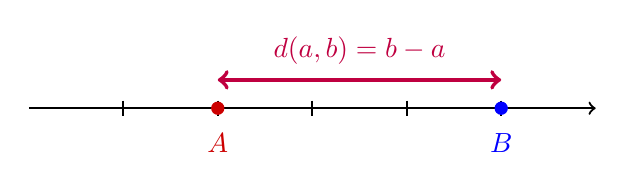
\begin{tikzpicture}[scale=1.2]
			\draw[->, thick] (-1,0) -- (5,0);
			\foreach \x in {0,1,2,3,4} { \draw[thick] (\x,0.08) -- (\x,-0.08); }
			\fill[red!80!black] (1,0) circle (2pt) node[below=2mm] {$A$};
			\fill[blue] (4,0) circle (2pt) node[below=2mm] {$B$};
			\draw[<->, line width=1.5pt, purple] (1,0.3) -- (4,0.3);
			\node[purple, above=2pt] at (2.5,0.3) {$d(a,b) = \abs{b - a}$};
		\end{tikzpicture}
	\end{center}
\end{df}

\begin{remarque}
	En particulier, pour tout réel $x$, la valeur absolue $\abs{x} = \abs{x - 0} = d(x,0)$ représente la \textbf{distance entre $x$ et l'origine $0$}.
\end{remarque}

\subsection{Équations et inéquations avec valeur absolue}

\begin{prop}[Résolution d'équations $\abs{x - a} = r$]
	Soient $a \in \R$ et $r \geqslant 0$.

	L'équation $\abs{x - a} = r$ signifie que la distance entre $x$ et $a$ est égale à $r$.
	\[
		\abs{x - a} = r \iff \begin{cases}x_1 = a - r \\ x_2 = a + r\end{cases}
	\]
\end{prop}

\newpage

\begin{ex}
	Résolvons dans $\R$ l'équation $\abs{x - 2} = 3$.

	\textbf{Interprétation :} On cherche les réels $x$ situés à une distance de $3$ du point d'abscisse $2$.

	\begin{center}
		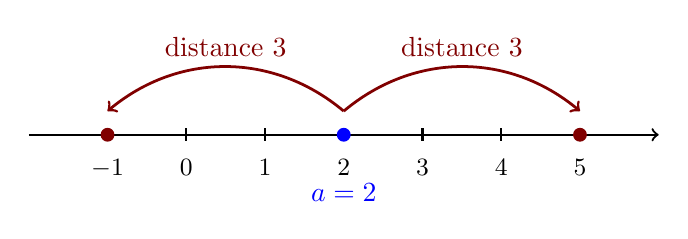
\begin{tikzpicture}[scale=1]
			\draw[->, thick] (-2,0) -- (6,0);
			\foreach \x in {-1,0,1,2,3,4,5} { \draw[thick] (\x,0.08) -- (\x,-0.08) node[below=1mm] {\small $\x$}; }
			\fill[blue] (2,0) circle (2.5pt) node[below=5mm] {$a = 2$};
			\draw[->, line width=1pt, red!50!black] (2,0.3) to[out=140,in=40] node[midway,above] {distance $3$} (-1,0.3);
			\draw[->, line width=1pt, red!50!black] (2,0.3) to[out=40,in=140] node[midway,above] {distance $3$} (5,0.3);
			\fill[red!50!black] (-1,0) circle (2.5pt);
			\fill[red!50!black] (5,0) circle (2.5pt);
		\end{tikzpicture}
	\end{center}

	L'ensemble des solutions est $S = \{-1 \,;\, 5\}$.
\end{ex}

\begin{prop}[Résolution d'inéquations $\abs{x - a} \leqslant r$]
	Soient $a \in \R$ et $r \geqslant 0$.

	L'inéquation $\abs{x - a} \leqslant r$ signifie que la distance entre $x$ et $a$ est inférieure ou égale à $r$.
	\begin{align*}
		\abs{x - a} \leqslant r & \iff x \in \intff{\pa{a - r}}{\pa{a + r}}        \\
		                        & \iff \pa{a - r} \leqslant x \leqslant \pa{a + r}
	\end{align*}
\end{prop}

\begin{ex}
	Résolvons dans $\R$ l'inéquation $\abs{x - 2} \leqslant 3$.

	\textbf{Interprétation :} On cherche les réels $x$ dont la distance à $2$ est inférieure ou égale à $3$.

	\begin{center}
		\begin{tikzpicture}[scale=1]
			\draw[->, thick] (-2.5,0) -- (6.5,0);
			\foreach \x in {-2,-1,0,1,3,4,5,6} { \draw[thick] (\x,0.08) -- (\x,-0.08) node[below=1mm] {\small $\x$}; }
			\draw[blue, line width=1.5pt, {Bracket[length=4pt, width=13pt]}-{Bracket[length=4pt, width=13pt]}] (-1.03,0) -- (5.03,0);
			\node[blue, above=6pt] at (2,0) {$\intff{-1}{5}$};
			\fill (2,0) circle (2pt) node[below=2mm] {$a = 2$};
			\draw[<->, thick, red!50!black] (-1,-1) -- (2,-1) node[midway,below] {$r=3$};
			\draw[<->, thick, red!50!black] (2,-1) -- (5,-1) node[midway,below] {$r=3$};
		\end{tikzpicture}
	\end{center}

	L'ensemble des solutions est l'intervalle $S = \intff{-1}{5}$.
\end{ex}

\newpage
\section{Exercices}
 {\small
  \begin{multicols}{2}
	  \begin{exo}{}
	Compléter le schéma ci-dessous en associant à chaque zone le symbole de l'ensemble de nombres qui convient.

	\begin{center}
		\begin{tikzpicture}[scale=0.8, every node/.style={scale=0.9}]
			\draw[thick, fill=blue!5] (0,0) ellipse (4.5cm and 3.3cm);
			\draw[thick, fill=green!8!white] (-0.3,0) ellipse (3.4cm and 2.6cm);
			\draw[thick, fill=orange!12!white] (-0.6,0) ellipse (2.4cm and 2.1cm);
			\draw[thick, fill=purple!10!white] (-0.9,0) ellipse (1.5cm and 1.5cm);
			\draw[thick, fill=gray!20!white] (-1.2,0) ellipse (0.7cm and 1.0cm);
			\node[fill=white, inner sep=6pt, scale=0.8] at (-1.2,0) {\ \dots\ };
			\node[fill=white, inner sep=6pt, scale=0.8] at (0,0) {\ \dots\ };
			\node[fill=white, inner sep=6pt, scale=0.8] at (1.1,0) {\ \dots\ };
			\node[fill=white, inner sep=6pt, scale=0.8] at (2.3,0) {\ \dots\ };
			\node[fill=white, inner sep=6pt, scale=0.8] at (3.7,0) {\ \dots\ };
			\node[scale=1.2, black] at (-1.2,-0.7) {$7$};
			\node[scale=1.2, black] at (-0.3,0.65) {$-3$};
			\node[scale=1.2, black] at (0.9,-0.9) {$-0,5$};
			\node[scale=1.2, black] at (2.0,1.2) {$\dfrac{2}{3}$};
			\node[scale=1.2, black] at (3.2,-1.4) {$\sqrt{2}$};
		\end{tikzpicture}
	\end{center}
\end{exo}

	  \begin{exo}{}
	Pour chaque affirmation, indiquer si elle est \textbf{Vraie} ou \textbf{Fausse} en justifiant la réponse. (Si une affirmation est fausse, on donnera un contre-exemple).

	\begin{enumerate}[label=\arabic*), itemsep=5pt]
		\item Si un nombre appartient à l'ensemble $\mathbb{N}$, alors il appartient à l'ensemble $\mathbb{R}$.
		\item Si un nombre appartient à l'ensemble $\mathbb{D}$, alors il appartient à l'ensemble $\mathbb{Z}$.
		\item Tout nombre rationnel est un nombre réel.
		\item Si $x \in \mathbb{R}$ et $x \notin \mathbb{Q}$, alors $x$ est forcément un nombre décimal.
		\item Si un nombre entier relatif n'est pas un nombre naturel, alors il est strictement négatif.
		\item Le quotient de deux entiers relatifs est toujours un nombre décimal.
	\end{enumerate}
\end{exo}

	  \begin{exo}{}
	Compléter les pointillés par le symbole d'inclusion qui convient ($\subset$ ou $\not\subset$) :
	\begin{multicols}{2}
	\begin{enumerate}[label=\alph*), itemsep=4pt]
		\item $\mathbb{N} \ \dots \ \mathbb{Z}$
		\item $\mathbb{Q} \ \dots \ \mathbb{D}$
		\item $\mathbb{Z} \ \dots \ \mathbb{R}$
		\item $\mathbb{D} \ \dots \ \mathbb{Q}$
	\end{enumerate}
	\end{multicols}
\end{exo}

	  \begin{exo}{}
	Compléter les pointillés par le symbole qui convient ($\in$ ou $\notin$).
	\begin{multicols}{2}
	\begin{enumerate}[label=\alph*), itemsep=6pt]
		\item $-7 \ \dots \ \mathbb{R}$
		\item $14,4432 \ \dots \ \mathbb{D}$
		\item $\dfrac{17}{3} \ \dots \ \mathbb{Q}$
		\item $\dfrac{3}{4} \ \dots \ \mathbb{Q}$
		\item $-\dfrac{6}{7} \ \dots \ \mathbb{R}$
		\item $\sqrt{4} \ \dots \ \mathbb{Z}$
		      % \item $-\sqrt{144} \ \dots \ \mathbb{Z}$
		      % \item $-17,2 \ \dots \ \mathbb{Q}$
		      % \item $\dfrac{10}{3} \ \dots \ \mathbb{D}$
	\end{enumerate}
	\end{multicols}
\end{exo}

	  \vfill~\columnbreak
	  \begin{exo}{}
	Après éventuelle simplification, compléter les pointillés par le symbole qui convient ($\in$ ou $\notin$).

	On admet que $\sqrt{2}$ et $\pi$ sont des irrationnels.
	\begin{multicols}{2}
	\begin{enumerate}[label=\alph*), itemsep=8pt]
		\item $-\dfrac{18}{6} \ \dots \ \mathbb{Z}$
		\item $\dfrac{-16\pi}{-2\pi} \ \dots \ \mathbb{N}$
		\item $\dfrac{\pi+1}{\pi+3} \ \dots \ \mathbb{Q}$
		\item $-3\sqrt{2} + 1 \ \dots \ \mathbb{Q}$
	\end{enumerate}
	\end{multicols}
\end{exo}

	  \begin{exo}{}
	Donner le plus petit ensemble ($\mathbb{N}$, $\mathbb{Z}$, $\mathbb{D}$, $\mathbb{Q}$ ou $\mathbb{R}$) auquel appartient chaque nombre ci-dessous :
	\begin{multicols}{2}
	\begin{enumerate}[label=\alph*), itemsep=6pt]
		\item $7,141\,414 \in \ \dots$
		\item $\dfrac{22}{11} \in \ \dots$
		\item $-\dfrac{84}{14} \in \ \dots$
		\item $\sqrt{121} \in \ \dots$
		\item $-\dfrac{153}{3} \in \ \dots$
		\item $\dfrac{11}{3} \in \ \dots$
		\item $-\dfrac{25}{\sqrt{100}} \in \ \dots$
		\item $0,333 \in \ \dots$
		      % \item $0,\underline{45} \in \ \dots$ \hfill \small{(le nombre 45 se répète sans fin)}
	\end{enumerate}
	\end{multicols}
\end{exo}

	  \begin{exo}{}
	Quel est le plus petit ensemble de nombres auquel appartient chacun des nombres suivants ?
	\vspace*{-2mm}\begin{multicols}{2}
	\begin{enumerate}
		\item $\dfrac{1}{2}$
		\item $\sqrt{5}$
		\item $\dfrac{10 - 4}{3}$
		\item $-\sqrt{16}$
	\end{enumerate}
	\end{multicols}\vspace*{-2mm}
\end{exo}

	  \begin{exo}{}
	Quel est le plus petit ensemble de nombres auquel appartient chacun des nombres suivants ?
	\vspace*{-2mm}
	\begin{multicols}{2}
		\begin{enumerate}
			\item $\dfrac{1}{2} + \dfrac{1}{3} + \dfrac{1}{6}$
			\item $\sqrt{16} - \sqrt{25}$
			\item $\dfrac{91}{7}$
			\item $\dfrac{34}{2} - \sqrt{289}$
		\end{enumerate}
	\end{multicols}\vspace*{-2mm}
\end{exo}

	  \begin{exo}{}
	Lesquels de ces nombres sont décimaux ?
	\vspace*{-2mm}
	\begin{multicols}{2}
	\begin{enumerate}
		\item $-5$
		\item $\dfrac{40}{3}$
		\item $\dfrac{3}{40}$
		\item $\dfrac{5}{7}$
	\end{enumerate}
	\end{multicols}\vspace*{-2mm}
\end{exo}

	  \begin{exo}{}
	Pour chacune des affirmations suivantes, dire si elle est toujours vraie. Si elle est fausse, donner un contre-exemple.
	\begin{enumerate}
		\item La différence de deux nombres entiers naturels est un entier naturel.
		\item Le quotient de deux nombres décimaux est un nombre décimal.
		\item Le quotient de deux nombres réels est un nombre rationnel.
		\item Le produit d'un nombre rationnel par un nombre entier relatif est un nombre rationnel.
	\end{enumerate}
\end{exo}

	  \vfill~\columnbreak
	  \begin{exo}{}
	Compléter les pointillés par $\in$ ou $\notin$.
	\vspace*{-2mm}\begin{multicols}{2}
	\begin{enumerate}[itemsep=2mm]
		\item $-3 \ \dots \ \intfo{-5}{-1}$
		\item $\dfrac{-26}{5} \ \dots \ \intoo{-5}{-4}$
		\item $2\pi \ \dots \ \intoo{7}{8}$
		\item $0 \ \dots \ \intoo{-\infty}{+\infty}$
		\item $-2 \ \dots \ \intfo{2}{1}$
		\item $4 \ \dots \ \intfo{-3}{4}$
	\end{enumerate}
	\end{multicols}\vspace*{-2mm}
\end{exo}

	  \begin{exo}{}
	Recopier et compléter avec $\in$ ou $\notin$.
	\vspace*{-2mm}\begin{multicols}{2}
	\begin{enumerate}[itemsep=2mm]
		\item $2$ \dots $\intoo{1}{3}$
		\item $0$ \dots $\intfo{-1}{2}$
		\item $\frac{1}{3}$ \dots $\intff{0}{3}$
		\item $2$ \dots $\intoo{-2}{2}$
		\item $\sqrt{2}$ \dots $\intff{-3}{1}$
		\item $0$ \dots $\intoo{0}{+\infty}$
		\item $-100$ \dots $\intoo{-\infty}{1}$
		\item $\frac{1}{10}$ \dots $\intfo{0,01}{0,2}$
	\end{enumerate}
	\end{multicols}\vspace*{-2mm}
\end{exo}

	  \begin{exo}{}
	Écrire sous forme d'intervalles les représentations graphiques suivantes :
	\begin{enumerate}
		\item
		      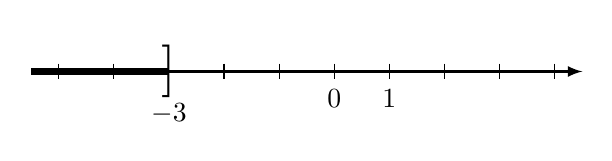
\begin{tikzpicture}[baseline=(current bounding box.center), scale=0.7, >=latex]
			      \draw[->, thick] (-5.5,0) -- (4.5,0);
			      \foreach \x in {-5,-4,-3,-2,-1,0,1,2,3,4} \draw (\x,4pt) -- (\x,-4pt);
			      \node[below=1pt] at (0,-0.1) {$0$};
			      \node[below=1pt] at (1,-0.10) {$1$};
			      \node[below=6pt] at (-3,-0.10) {$-3$};
			      \draw[ultra thick, line width=2.5pt] (-5.5,0) -- (-3,0);
			      \node[thick, scale=1.9, text=black] at (-3,0) {$]$};
		      \end{tikzpicture}

		\item
		      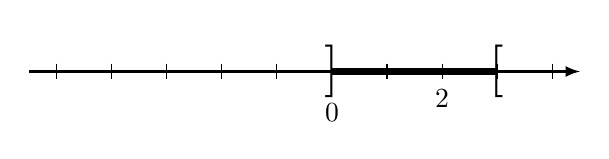
\begin{tikzpicture}[baseline=(current bounding box.center), scale=0.7, >=latex]
			      \draw[->, thick] (-5.5,0) -- (4.5,0);
			      \foreach \x in {-5,-4,-3,-2,-1,0,1,2,3,4} \draw (\x,4pt) -- (\x,-4pt);
			      \node[below=6pt] at (0,-0.10) {$0$};
			      \node[below=1pt] at (2,-0.10) {$2$};
			      \draw[ultra thick, line width=2.5pt] (0,0) -- (3,0);
			      \node[thick, scale=1.9, text=black] at (0,0) {$]$};
			      \node[thick, scale=1.9, text=black] at (3,0) {$[$};
		      \end{tikzpicture}

		\item
		      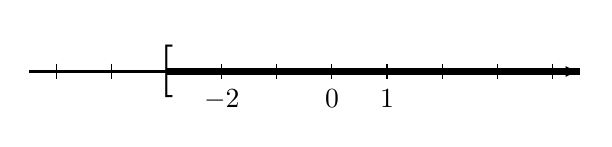
\begin{tikzpicture}[baseline=(current bounding box.center), scale=0.7, >=latex]
			      \draw[->, thick] (-5.5,0) -- (4.5,0);
			      \foreach \x in {-5,-4,-3,-2,-1,0,1,2,3,4} \draw (\x,4pt) -- (\x,-4pt);
			      \node[below=1pt] at (0,-0.10) {$0$};
			      \node[below=1pt] at (1,-0.10) {$1$};
			      \node[below=1pt] at (-2,-0.10) {$-2$};
			      \draw[ultra thick, line width=2.5pt] (-3,0) -- (4.5,0);
			      \node[thick, scale=1.9, text=black] at (-3,0) {$[$};
		      \end{tikzpicture}
	\end{enumerate}
\end{exo}

	  \begin{exo}{}
	Compléter les équivalences suivantes :
	\begin{enumerate}[itemsep=3mm]
		\item $-1 \leq x \leq 5$ équivaut à $x \in \ \dots$
		\item $\dots \ x \ \dots$ équivaut à $x \in [0\ ;\ 4]$
		\item $2 < x < \dfrac{7}{2}$ équivaut à $x \in \ \dots$
		\item $\dots \ x \ \dots$ équivaut à $x \in [-2\ ;\ 1[$
		\item $-5 \leq x < 0$ équivaut à $x \in \ \dots$
	\end{enumerate}
\end{exo}

	  \begin{exo}{}
	Compléter le tableau comme dans l'exemple.

	\renewcommand{\arraystretch}{1.5}
	\begin{center}
		\begin{tabular}{|c|c|C{4cm}|} \hline
			\rowcolor{orange!80} \textbf{\color{white}\small Inégalité} & \textbf{\color{white}\small Intervalle} & \textbf{\color{white}\small Représentation graphique} \\ \hline
			$2 \le x \le 4$                                             & $x \in \intff{2}{4}$                    &
			\begin{tikzpicture}[scale=0.6, >=Stealth, baseline={([yshift=-0.7ex]current bounding box.center)}]
				\draw[->, thick] (0.5,0) -- (5.5,0);
				\foreach \x in {1,2,3,4,5} \draw (\x,0.1) -- (\x,-0.1);
				\node[below=1mm, scale=0.8] at (1,0) {$1$};
				\node[below=1mm, scale=0.8] at (3,0) {$3$};
				\node[below=1mm, scale=0.8] at (5,0) {$5$};
				\draw[line width=2pt, blue, {Bracket[width=5mm, length=1mm]}-{Bracket[width=5mm, length=1mm]}] (1.9,0) -- (4.1,0);
				\draw[line width=2pt, white] (0,0.8) -- (4,0.8);
				% \node[above=3mm, scale=0.8] at (2,0) {$2$};
				% \node[above=3mm, scale=0.8] at (4,0) {$4$};
			\end{tikzpicture}                                              \\ \hline
			$0 < x \le 5$                                               & \phantom{$x \in \intof{0}{5}$}          &                                                       \\ \hline
			\phantom{$2 \le x \le 4$}                                   & \phantom{$x \in \intff{2}{4}$}          &
			\begin{tikzpicture}[scale=0.45, >=Stealth, baseline={([yshift=-0.7ex]current bounding box.center)}]
				\draw[->, thick] (-3.5,0) -- (4.5,0);
				\foreach \x in {-3,-2,-1,0,1,2,3,4} \draw (\x,0.1) -- (\x,-0.1);
				\node[below=1mm, scale=0.8] at (-3,0) {$-3$};
				\node[below=1mm, scale=0.8] at (-2,0) {$-2$};
				\node[below=1mm, scale=0.8] at (0,0) {$0$};
				\node[below=1mm, scale=0.8] at (2,0) {$2$};
				\node[below=1mm, scale=0.8] at (3,0) {$3$};
				\node[below=1mm, scale=0.8] at (4,0) {$4$};
				\draw[line width=2pt, blue, {Bracket[width=5mm, length=1mm,reversed]}-{Bracket[width=5mm, length=1mm]}] (-1.2,0) -- (1.1,0);
				\draw[line width=2pt, white] (0,0.8) -- (4,0.8);
				% \node[above=3mm, scale=0.8] at (1,0) {$1$};
				% \node[above=3mm, scale=0.8] at (-1,0) {$-1$};
			\end{tikzpicture}                                             \\ \hline
			                                                            & $x \in \intof{-\infty}{4}$              &                                                       \\ \hline
			$3 \le x$                                                   &                                         &                                                       \\ \hline
			                                                            & $x \in \intoo{-3}{7}$                   &                                                       \\ \hline
			                                                            &                                         &
			\begin{tikzpicture}[scale=0.45, >=Stealth, baseline={([yshift=-0.7ex]current bounding box.center)}]
				\draw[->, thick] (-3.5,0) -- (4.5,0);
				\foreach \x in {-3,-2,-1,0,1,2,3,4} \draw (\x,0.1) -- (\x,-0.1);
				\node[below=1mm, scale=0.8] at (-3,0) {$-3$};
				\node[below=1mm, scale=0.8] at (-2,0) {$-2$};
				\node[below=1mm, scale=0.8] at (0,0) {$0$};
				\node[below=1mm, scale=0.8] at (-1,0) {$-1$};
				\node[below=1mm, scale=0.8] at (1,0) {$1$};
				\node[below=1mm, scale=0.8] at (3,0) {$3$};
				\node[below=1mm, scale=0.8] at (4,0) {$4$};
				\draw[line width=2pt, blue, {Bracket[width=5mm, length=1mm]}-] (1.9,0) -- (4.5,0);
				\draw[line width=2pt, white] (0,0.8) -- (4,0.8);
				% \node[above=3mm, scale=0.8] at (2,0) {$2$};
			\end{tikzpicture}                                                                       \\ \hline
		\end{tabular}
	\end{center}
\end{exo}

	  \vfill~\columnbreak
	  \begin{exo}{}
	Déterminer les intersections d'intervalles :
	\vspace*{-2mm}\begin{multicols}{2}
	\begin{enumerate}[label=\alph*), itemsep=6pt]
		\item $\intff{0}{2} ~\cap~ \intoo{1}{5}$
		\item $\intof{-\infty}{3} ~\cap~ \intff{4}{7}$
		\item $\intof{5}{6} ~\cap~ \intfo{-2}{7}$
		\item $\intof{-1}{5} ~\cap~ \intoo{5}{+\infty}$
		\item $\intof{-\infty}{1} ~\cap~ \intfo{1}{+\infty}$
	\end{enumerate}
	\end{multicols}\vspace*{-2mm}
\end{exo}

	  \begin{exo}{}
	Déterminer les réunions d'intervalles :
	\vspace*{-2mm}\begin{multicols}{2}
	\begin{enumerate}[label=\alph*), itemsep=6pt]
		\item $\intof{-\infty}{4} ~\cup~ \intoo{3}{+\infty}$
		\item $\intof{-2}{3} ~\cup~ \intff{-5}{7}$
		\item $\intof{-4}{3} ~\cup~ \intfo{2}{+\infty}$
		\item $\intof{-8}{-5} ~\cup~ \intff{0}{1}$
	\end{enumerate}
	\end{multicols}\vspace*{-2mm}
\end{exo}

	  \begin{exo}{}
	Chaque assertion suivante est supposée vraie.

	Dans chaque cas, écrire, sous forme d'intervalle ou de réunion d'intervalles, le plus grand ensemble auquel appartient $x$.

	\begin{enumerate}[itemsep=2mm]
		\item $x \ge 3$ ou $x \le 0$
		\item $x - 6 > 0$ ou $5x \le 5$
		\item $x \le 2$ ou $-4x \le -20$
		\item $x \ge 3$ ou $3x \ge 12$
		\item $7x - 4 \ge 3$ ou $1 - x > 0$
		\item $1 - x > -3$ ou $2x + 1 \le 7$
	\end{enumerate}
\end{exo}

	  \begin{exo}{}
	Écrire chaque condition sous forme d'intersection et trouver l'ensemble des réels $a$ appartenant à cette intersection.

	\begin{enumerate}[itemsep=2mm]
		\item $a < 3\quad$ et $\quad a > -6$
		\item $a \ge -5\quad$ et $\quad -a \ge -7$
		\item $2a + 1 < 3\quad$ et $\quad 3a - 1 \ge 0$
		\item $3(2 - a) < 3\quad$ et $\quad a - 1 \ge 2$
	\end{enumerate}
\end{exo}

	  \begin{exo}{}
	Dans la boîte de nuit le Macumba, il faut avoir strictement plus de $32$ ans pour entrer.

	Dans la boîte de nuit la Playa, il faut avoir au plus $40$ ans.
	\begin{enumerate}
		\item Dans quel intervalle d'âge doit se situer une personne qui veut pouvoir rentrer dans les deux boîtes de nuit ?
		\item Dans quel ensemble doit se situer l'âge d'une personne qui veut pouvoir entrer dans l'une des deux boîtes de nuit ?
	\end{enumerate}
\end{exo}

	  \begin{exo}{}
	L'Insee estime qu'un couple avec deux enfants appartient à la classe moyenne quand les revenus du foyer sont situés dans l'intervalle $\intff{\np{3253}}{\np{5609}}$.

	M. Martin gagne $\np{2731}\eur{}$ et Mme Martin gagne $\np{2732}\eur{}$.

	Ils ont deux enfants qui ne rapportent aucun revenu. La famille appartient-elle à la classe moyenne ?
\end{exo}

	  \vfill~\columnbreak
	  \begin{exo}{}
	Résoudre les inéquations suivantes dans $\R$.
	\vspace*{-2mm}\begin{multicols}{2}
	\begin{enumerate}[itemsep=2mm]
		\item $2x + 1 > 3$
		\item $3x - 2 \le 7$
		\item $-5x + \frac{1}{2} \ge 3$
		\item $2 - x < 5$
	\end{enumerate}
	\end{multicols}\vspace*{-2mm}
\end{exo}

	  \begin{exo}{}
	Résoudre les inéquations suivantes dans $\R$.
	\vspace*{-2mm}\begin{multicols}{2}
	\begin{enumerate}[itemsep=2mm]
		\item $7x + 3 > 2x - 5$
		\item $5x - 3 \le 8x - 6$
		\item $7(x + 1) > 5 - 2x$
		\item $-5x + 3 \ge 2(x - 5)$
	\end{enumerate}
	\end{multicols}\vspace*{-2mm}
\end{exo}

	  \begin{exo}{}
	On considère les trois intervalles suivants :
	\cmath{I = \intfo{-4}{2}\ ,\ J = \intoo{-1}{5}\ \text{ et }\ K = \intff{0}{3}}
	\begin{enumerate}
		\item Représenter ces trois intervalles sur un même axe gradué.
		\item Déterminer l'intervalle correspondant à l'intersection des trois ensembles, noté $I \cap J \cap K$.
		\item Déterminer l'ensemble des réels $x$ qui appartiennent à $I \cup J$ mais qui n'appartiennent pas à $K$. Écrire le résultat sous la forme d'une réunion d'intervalles.
	\end{enumerate}
\end{exo}

	  \begin{exo}{}
	On considère le triangle ci-dessous, dans lequel les côtés dépendent d'un nombre réel $x > 1$.

	\begin{center}
		\begin{tikzpicture}[scale=0.9, >=Stealth]
			\coordinate (A) at (0,0);
			\coordinate (B) at (6,0);
			\coordinate (C) at (4,3);
			\draw[very thick] (A) -- (B) node[midway, below=1mm] {$2x - 1$} -- (C) node[midway, above right=1mm] {$3x + 6$} -- cycle node[midway, above left=1mm] {$x + 9$};
			\node[left=1mm] at (A) {$A$};
			\node[right=1mm] at (B) {$B$};
			\node[above=1mm] at (C) {$C$};
		\end{tikzpicture}
	\end{center}
	\begin{enumerate}
		\item Pour quelle valeur de $x$ a-t-on $AB = AC$ ? Pour cette valeur de $x$, quelle est la longueur de chacun des côtés de $ABC$ ?
		\item Déterminer toutes les valeurs de $x$ pour lesquelles le triangle $ABC$ est isocèle.
		\item Peut-on trouver une valeur de $x$ pour laquelle le triangle $ABC$ est équilatéral ?
	\end{enumerate}
\end{exo}

	  \vfill~\columnbreak
	  \begin{exo}{}
	Trois étudiants, Alice, Bob et Chloé, doivent se retrouver à la bibliothèque universitaire pour travailler sur un projet de mathématiques.

	La bibliothèque est ouverte en continu de $8h$ à $18h$.

	Chaque étudiant a des disponibilités bien précises au cours de cette journée :
	\begin{itemize}
		\item Alice est disponible entre $9h$ et $14h$.
		\item Bob est disponible à partir de $11h$ jusqu'à $16h$.
		\item Chloé est disponible soit entre $8h30$ et $10h$, soit entre $13h$ et $17h$.
	\end{itemize}
	\begin{enumerate}
		\item Écrirer les plages horaires de disponibilité d'Alice, de Bob et de Chloé sous la forme d'intervalles ou de réunions d'intervalles, que l'on notera respectivement $A$, $B$ et $C$.
		\item Représenter ces trois ensembles sur un même axe gradué en utilisant trois couleurs différentes.
		\item Alice et Bob décident de commencer à travailler ensemble en attendant Chloé.
		      \begin{enumerate}
			      \item Traduire mathématiquement leur plage horaire commune à l'aide d'un symbole d'opération sur les ensembles.
			      \item Déterminer cet ensemble sous forme d'intervalle, puis le traduire par une phrase claire en donnant les horaires correspondants.
		      \end{enumerate}
		\item Déterminer l'ensemble $A \cap B \cap C$. Que représente cet ensemble pour les trois étudiants ? Est-il possible qu'ils se réunissent tous les trois en même temps ?
		\item Déterminer l'ensemble $A \cup B$. À quoi correspond cet ensemble dans le contexte de l'exercice ?
	\end{enumerate}
\end{exo}

	  \vfill~
  \end{multicols}
 }

\chapter{Équations et inéquations}

\section{Équations}

\subsection{Équations du premier degré}

\begin{methode}[Résoudre une équation du premier degré]
	Résoudre :
	\begin{multicols}{3}
		\begin{itemize}
			\item $-5x + 3 = -3x + 2$
			\item $3(x + 4) = -(x + 5) + 2$
		\end{itemize}
	\end{multicols}

	\begin{correction}
		\[
			\begin{array}{ll}%
				\def\arraystretch{1.2}%
				\begin{array}{rrcl}%
					     & -5x + 3  & = & -3x + 2                       \\
					\eqv & -5x + 3x & = & 2 - 3                         \\
					\eqv & -2x      & = & -1                            \\
					\eqv & x        & = & \dfrac{-1}{-2} = \dfrac{1}{2} \\
					     &          &   &
				\end{array} \qquad & \qquad %
				\def\arraystretch{1.2}%
				\begin{array}{rrcl}%
					     & 3(x + 4) & = & -(x + 5) + 2   \\
					\eqv & 3x + 12  & = & -x - 5 + 2     \\
					\eqv & 3x + x   & = & -12 - 5 + 2    \\
					\eqv & 4x       & = & -15            \\
					\eqv & x        & = & -\dfrac{15}{4}
				\end{array}%
			\end{array}%
		\]
	\end{correction}
\end{methode}

\subsection{Équation produit}

\begin{prop}[Règle du produit nul]
	Un produit de facteurs est nul \textbf{si et seulement si} l'un au moins de ses facteurs est nul.

	\[
		A \times B = 0 \iff A = 0 \quad \text{ou} \quad B = 0
	\]
\end{prop}

\begin{methode}[Résoudre une équation produit]
	Résoudre dans $\mathbb{R}$ :
	\begin{multicols}{3}
		\begin{itemize}
			\item $(4x + 6)(3 - 7x) = 0$
			\item $5x^2 - 4x = 0$
		\end{itemize}
	\end{multicols}

	\begin{correction}
		\nline
		\begin{itemize}
			\item $(4x + 6)(3 - 7x) = 0$

			      \[
				      \begin{array}{rcl}
					      (4x + 6)(3 - 7x) = 0 & \iff & \begin{cases}
						                                    4x + 6 = 0 \\
						                                    3 - 7x = 0
					                                    \end{cases} \iff \begin{cases}
						                                                     4x = -6 \\
						                                                     -7x = -3
					                                                     \end{cases} \iff \begin{cases}
						                                                                      x = \dfrac{-6}{4} = \dfrac{-3}{2} \\[3mm]
						                                                                      x = \dfrac{3}{7}
					                                                                      \end{cases} \\ %
					                           & \iff & S = \brac{\dfrac{-3}{2}\ ;\ \dfrac{3}{7}}
				      \end{array}
			      \]

			\item $5x^2 - 4x = 0$

			      On factorise par $x$ pour obtenir un produit.

			      \[
				      \begin{array}{rcl}
					      5x^2 - 4x = 0 & \iff & x(5x - 4) = 0 \iff \begin{cases}
						                                                x = 0 \\
						                                                5x - 4 = 0
					                                                \end{cases} \iff \begin{cases}
						                                                                 x = 0 \\
						                                                                 5x = 4
					                                                                 \end{cases} \iff \begin{cases}
						                                                                                  x = 0 \\[1mm]
						                                                                                  x = \dfrac{4}{5}
					                                                                                  \end{cases} \\[3mm] %
					                    & \iff & S = \brac{0\ ;\ \dfrac{4}{5}}
				      \end{array}
			      \]
		\end{itemize}
	\end{correction}
\end{methode}

\subsection{Équation quotient}

\begin{prop}[Règle du quotient nul]
	Un quotient est nul \textbf{si et seulement si} son numérateur est nul \textbf{et} son dénominateur est non nul.

	\[
		\dfrac{A}{B} = 0 \iff A = 0 \quad \text{et} \quad B \neq 0
	\]
\end{prop}

\begin{ex}
	Soit l'équation : $\quad\dfrac{x+2}{x+3} = 0$

	\begin{itemize}
		\item \textbf{Condition d'existence :} L'expression est définie pour $x + 3 \neq 0$, c'est-à-dire $x \neq -3$.
		\item \textbf{Résolution :} Pour tout $x \neq -3$,
		      \[
			      \dfrac{x+2}{x+3} = 0 \iff x + 2 = 0 \iff x = -2
		      \]
		\item \textbf{Conclusion :} Comme $-2 \neq -3$, la solution est $S = \{-2\}$.
	\end{itemize}
\end{ex}

\begin{methode}[Résoudre une équation quotient]
	Résoudre dans $\mathbb{R}$ :
	\begin{multicols}{3}
		\begin{enumerate}
			\item $\dfrac{3x+5}{x-1} = 0$
			\item $\dfrac{(2x+1)(x-3)}{x-4} = 0$
		\end{enumerate}
	\end{multicols}

	\begin{correction}
		\nline
		\begin{itemize}
			\item $\dfrac{3x+5}{x-1} = 0$
			      \[
				      \begin{array}{rcl}
					      \dfrac{3x+5}{x-1} = 0 & \iff & \begin{cases}
						                                     3x + 5 = 0 \\
						                                     x - 1 \neq 0
					                                     \end{cases} \iff \begin{cases}
						                                                      3x = -5 \\
						                                                      x \neq 1
					                                                      \end{cases} \iff \begin{cases}
						                                                                       x = -\dfrac{5}{3} \\[1mm]
						                                                                       x \neq 1
					                                                                       \end{cases} \\ %
					                            & \iff & S = \brac{-\dfrac{5}{3}}
				      \end{array}
			      \]

			\item $\dfrac{(2x+1)(x-3)}{x-4} = 0$
			      \[
				      \begin{array}{rcl}
					      \dfrac{(2x+1)(x-3)}{x-4} = 0 & \iff & \begin{cases}
						                                            (2x + 1)(x - 3) = 0 \\
						                                            x - 4 \neq 0
					                                            \end{cases} \iff \begin{cases}
						                                                             2x + 1 = 0 \\
						                                                             x - 3 = 0  \\
						                                                             x \neq 4
					                                                             \end{cases} \iff \begin{cases}
						                                                                              x = -\dfrac{1}{2} \\
						                                                                              x = 3             \\
						                                                                              x \neq 4
					                                                                              \end{cases} \\ %
					                                   & \iff & S = \brac{\dfrac{-1}{2} \,;\, 3}
				      \end{array}
			      \]
		\end{itemize}
	\end{correction}
\end{methode}

\subsection{Équation de la forme $x^2 = a$}

\begin{prop}[Solutions de $x^2 = a$]
	\nline
	\begin{itemize}
		\item Si $a < 0$ : l'équation n'a \textbf{pas de solution} dans $\mathbb{R}$.
		\item Si $a = 0$ : l'équation possède l'\textbf{unique solution} $x = 0$.
		\item Si $a > 0$ : l'équation possède \textbf{deux solutions} $x = -\sqrt{a}$ et $x = \sqrt{a}$.
	\end{itemize}
\end{prop}

\begin{demo}[Solutions de $x^2 = a$]
	\nline
	\begin{itemize}
		\item Si $a < 0$ : pas de solution car un carré est toujours positif.
		\item Si $a = 0$ : l'équation s'écrit $x^2 = 0$ donc $x = 0$.
		\item \textbf{Si $a > 0$ :} L'équation $x^2 = a$ admet deux solutions distinctes :
		      \[
			      \begin{array}{rcl}
				      x^2 = a & \iff & x^2 - a = 0                            \\[1mm]
				              & \iff & x^2 - \pa{\sqrt{a}}^2 = 0              \\[1mm]
				              & \iff & \pa{x - \sqrt{a}}\pa{x + \sqrt{a}} = 0 \\[2mm]
				              & \iff & \begin{cases}
					                       x - \sqrt{a} = 0 \\
					                       x + \sqrt{a} = 0
				                       \end{cases} \iff \begin{cases}
					                                        x = \sqrt{a} \\[1mm]
					                                        x = -\sqrt{a}
				                                        \end{cases}
			      \end{array}
		      \]
		      L'ensemble des solutions est donc $S = \brac{-\sqrt{a} \,;\, \sqrt{a}}$.
	\end{itemize}
\end{demo}

\begin{methode}[Résoudre une équation de la forme $x^2 = a$]
	Résoudre dans $\mathbb{R}$ :
	\begin{multicols}{3}
		\begin{itemize}
			\item $x^2 = 16$
			\item $x^2 = -8$
			\item $(x + 2)^2 = 9$
		\end{itemize}
	\end{multicols}

	\begin{correction}
		\nline
		\begin{itemize}
			\item $x^2 = 16$
			      \[
				      x^2 = 16
				      \iff \begin{cases}
					      x = -\sqrt{16} = -4 \\
					      x = \sqrt{16} = 4
				      \end{cases}
				      \iff S
				      = \{-4\ ;\ 4\}
			      \]

			\item $x^2 = -8$
			      \[
				      x^2 = -8 \iff S = \varnothing \quad \text{(un carré est toujours positif)}
			      \]

			\item $(x + 2)^2 = 9$
			      \[
				      (x + 2)^2 = 9
				      \iff \begin{cases}
					      x + 2 = -3 \\
					      x + 2 = 3
				      \end{cases}
				      \iff \begin{cases}
					      x = -5 \\
					      x = 1
				      \end{cases}
				      \iff S
				      = \{-5\ ;\ 1\}
			      \]
		\end{itemize}
	\end{correction}
\end{methode}

\section{Inéquations}

\subsection{Inéquations du premier degré}

\begin{defin}[Inéquation]
	Une \textbf{inéquation} est une inégalité contenant un nombre inconnu $x$.

	\textbf{Résoudre une inéquation}, c'est trouver toutes les valeurs de $x$ qui vérifient cette inégalité.

	Ces valeurs sont appelées les \textbf{solutions} de l'inéquation.
\end{defin}

\begin{ex}
	$2x + 1 > 4$ est une inéquation.

	Par exemple, $x = 10$ et $x = 2$ sont des solutions.
\end{ex}

\begin{attention}
	Lorsqu'on \textbf{multiplie} ou que l'on \textbf{divise} les deux membres d'une inéquation par un \textbf{nombre négatif}, on doit \textbf{changer le sens} de l'inégalité.
\end{attention}

\begin{ex}
	\[
		2 < 5 \quad \xrightarrow{\quad \text{multiplication par } -1 \quad} \quad - 2 > -5
	\]
\end{ex}

\newpage

\begin{methode}[Résoudre une inéquation du premier degré (1)]
	Résoudre et représenter les solutions sur une droite graduée :

	\[
		2x + 3 < 4 - 5x
	\]

	\begin{correction}
		\[
			\def\arraystretch{1.2}%
			\begin{array}{rrcl}%
				     & 2x + 3  & < & 4 - 5x       \\
				\iff & 2x + 5x & < & 4 - 3        \\
				\iff & 7x      & < & 1            \\
				\iff & x       & < & \dfrac{1}{7}
			\end{array}
		\]
		L'ensemble des solutions est $S = \intoo{-\infty}{\dfrac{1}{7}}$.

		\begin{center}
			\begin{tikzpicture}[xscale=4,yscale=0.5]
				\draw[-{Stealth[length=10pt, width=8pt]}, thick] (-0.5,0) -- (1.5,0);
				\foreach \x in {0,1} \draw[thick] (\x, -0.3) -- (\x, 0.3) node[below=8pt] {\x};
				\draw[red, line width=3pt, {-Bracket[reversed,width=15pt, length=5pt]}] (-0.5, 0) -- (1/7+0.05, 0);
				\node[above=8pt, red] at (1/7,0) {$\dfrac{1}{7}$};
			\end{tikzpicture}
		\end{center}
	\end{correction}
\end{methode}

\begin{methode}[Résoudre une inéquation du premier degré (2)]
	Résoudre et représenter les solutions sur une droite graduée :

	\[
		2(x - 4) \le 4x - 5
	\]

	\begin{correction}
		\[
			\def\arraystretch{1.2}%
			\begin{array}{rrcl}%
				     & 2(x - 4) & \le & 4x - 5                                                              \\
				\iff & 2x - 8   & \le & 4x - 5                                                              \\
				\iff & 2x - 4x  & \le & 8 - 5                                                               \\
				\iff & -2x      & \le & 3 \qquad \text{(division par } \pa{-2} \rarr \text{Le sens change)} \\
				\iff & x        & \ge & \dfrac{-3}{2}
			\end{array}
		\]
		L'ensemble des solutions est $S = \intfo{\dfrac{-3}{2}}{+\infty}$.

		\begin{center}
			\begin{tikzpicture}[xscale=1,yscale=0.5]
				\draw[-{Stealth[length=10pt, width=8pt]}, thick] (-4.5,0) -- (1.5,0);
				\foreach \x in {-4,-3,-2,-1,0,1} \draw[thick] (\x, -0.3) -- (\x, 0.3) node[below=8pt] {\x};
				\draw[red, line width=3pt, {Bracket[width=15pt, length=5pt]}-] (-1.5, 0) -- (1.5, 0);
				\node[above=8pt, red] at (-1.5,0) {$\dfrac{-3}{2}$};
			\end{tikzpicture}
		\end{center}
	\end{correction}
\end{methode}

\newpage

\subsection{Tableaux de signes}

\begin{defin}
	Un \textbf{tableau de signes} est un outil synthétique qui permet de visualiser immédiatement, selon les valeurs de l'inconnue $x$, si une expression mathématique est \textbf{positive} ($+$), \textbf{négative} ($-$) ou \textbf{nulle} ($0$).
\end{defin}

\begin{ex}{}
	Voici le tableau de signes d'une expression $A(x)$ définie sur $\mathbb{R}$ :
	\begin{center}
		\begin{tikzpicture}
			\tkzTabInit[lgt=2.5,espcl=2]{$x$ /1, $A(x)$ /1}{$-\infty$, $-1$, $4$, $+\infty$}
			\tkzTabLine{,-,z,+,z,-,}
		\end{tikzpicture}
	\end{center}

	L'expression $A(x)$ est strictement positive lorsque $x$ est compris entre $-1$ et $4$, c'est-à-dire pour $x \in ] - 1 \,;\, 4[$.

	\[
		A(x) \ge 0 \iff x \in \intff{-1}{4}
	\]

	Elle s'annule en $x = -1$ et $x = 4$.
\end{ex}

\begin{prop}[Signe de l'expression $ax + b$ (avec $a \neq 0$)]
	L'expression $ax + b$ s'annule pour $x = \frac{-b}{a}$.

	\begin{center}
		\begin{multicols}{2}
			\centering
			{$a > 0$}
			\vskip 2mm
			\begin{tikzpicture}
				\tkzTabInit[lgt=2,espcl=1.5]{$x$ /1, $ax + b$ /1}{$-\infty$, $\frac{-b}{a}$, $+\infty$}
				\tkzTabLine{,-,z,+,}
			\end{tikzpicture}

			\columnbreak

			\centering
			{$a < 0$}
			\vskip 2mm
			\begin{tikzpicture}
				\tkzTabInit[lgt=2,espcl=1.5]{$x$ /1, $ax + b$ /1}{$-\infty$, $\frac{-b}{a}$, $+\infty$}
				\tkzTabLine{,+,z,-,}
			\end{tikzpicture}
		\end{multicols}
	\end{center}
\end{prop}

\begin{demo}
	Pour déterminer le signe de $ax + b$ (avec $a \neq 0$), on cherche pour quelles valeurs de $x$ l'expression est strictement positive :
	\[
		ax + b > 0 \iff ax > -b
	\]
	Deux cas se présentent alors selon le signe du coefficient $a$ :

	\begin{itemize}
		\item \textbf{Si $a > 0$ :}

		      En divisant par $a$ sans changer le sens de l'inégalité, on obtient : $\quad x > \dfrac{-b}{a}$

		      L'expression $ax + b$ est donc strictement positive \textbf{après} $\dfrac{-b}{a}$ (et négative avant).

		\item \textbf{Si $a < 0$ :}

		      En divisant par $a$ (nombre négatif), le sens de l'inégalité change : $\quad x < \dfrac{-b}{a}$

		      L'expression $ax + b$ est donc strictement positive \textbf{avant} $\dfrac{-b}{a}$ (et négative après).
	\end{itemize}

	Ces résultats confirment la règle : l'expression $ax + b$ est du signe de $a$ après sa valeur d'annulation, ce qui valide les deux tableaux ci-dessus.
\end{demo}

\newpage

\begin{methode}[Tableau de signe d'une expression $ax + b$]
	Déterminer le tableau de signe de :
	\begin{multicols}{3}
		\begin{itemize}
			\item $2x + 6$
			\item $-3x + 12$
		\end{itemize}
	\end{multicols}
	\begin{correction}
		\nline
		\begin{multicols}{2}
			\begin{itemize}
				\item {Étude de $2x + 6$ :}
				      \[
					      \begin{aligned}
						      2x + 6 \ge 0 & \iff 2x \ge -6 \\
						                   & \iff x \ge -3
					      \end{aligned}
				      \]
				      L'expression est positive pour $x \ge -3$.

				      \begin{center}
					      \begin{tikzpicture}
						      \tkzTabInit[lgt=2.5,espcl=1.5]{$x$ /1, $2x + 6$ /1}{$-\infty$, $-3$, $+\infty$}
						      \tkzTabLine{,-,z,+,}
					      \end{tikzpicture}
				      \end{center}

				\item {Étude de $-3x + 12$ :}
				      \[
					      \begin{aligned}
						      -3x + 12 \ge 0 & \iff -3x \ge -12 \\
						                     & \iff x \le 4
					      \end{aligned}
				      \]
				      L'expression est positive pour $x \le 4$.

				      \begin{center}
					      \begin{tikzpicture}
						      \tkzTabInit[lgt=2.5,espcl=1.5]{$x$ /1, $-3x + 12$ /1}{$-\infty$, $4$, $+\infty$}
						      \tkzTabLine{,+,z,-,}
					      \end{tikzpicture}
				      \end{center}
			\end{itemize}
		\end{multicols}
	\end{correction}
\end{methode}

\begin{methode}[Tableau de signe d'un produit $(ax + b)(cx + d)$]
	Dresser le tableau de signe de :
	\[
		(3x - 9)(1 - 2x)
	\]

	\begin{correction}
		On étudie le signe de chaque facteur :
		\begin{multicols}{2}
			\begin{itemize}
				\item {Étude de $3x - 9$ :}
				      \[
					      \begin{aligned}
						      3x - 9 \ge 0 & \iff 3x \ge 9 \\
						                   & \iff x \ge 3
					      \end{aligned}
				      \]
				\item {Étude de $1 - 2x$ :}
				      \[
					      \begin{aligned}
						      1 - 2x \ge 0 & \iff -2x \ge -1         \\
						                   & \iff x \le \tfrac{1}{2}
					      \end{aligned}
				      \]
			\end{itemize}
		\end{multicols}

		\begin{center}
			\begin{tikzpicture}
				\tkzTabInit[lgt=4,espcl=2]
				{$x$ /1, $3x - 9$ /1, $1 - 2x$ /1, $(3x - 9)(1 - 2x)$ /1}
				{$-\infty$, $\frac{1}{2}$, $3$, $+\infty$}
				\tkzTabLine{,-,,-,z,+,}
				\tkzTabLine{,+,z,-,,-,}
				\tkzTabLine{,-,z,+,z,-,}
			\end{tikzpicture}
		\end{center}
		\textit{On applique la règle des signes pour déterminer le signe du produit.}
	\end{correction}
\end{methode}

\subsection{Inéquation produit}

\begin{methode}[Résoudre une inéquation produit]
	Résoudre dans $\mathbb{R}$ :
	\[
		(3 - 6x)(x + 2) > 0
	\]

	\begin{correction}
		Établissons le tableau de signe de $(3 - 6x)(x + 2)$ :

		\begin{multicols}{2}
			\begin{itemize}
				\item \textbf{Étude de $3 - 6x$ :}
				      \[
					      \begin{aligned}
						      3 - 6x \ge 0 & \iff -6x \ge -3         \\
						                   & \iff x \le \tfrac{1}{2}
					      \end{aligned}
				      \]

				\item \textbf{Étude de $x + 2$ :}
				      \[
					      \begin{aligned}
						      x + 2 \ge 0 & \iff x \ge -2
					      \end{aligned}
				      \]
			\end{itemize}
		\end{multicols}
		\begin{center}
			\begin{tikzpicture}
				\tkzTabInit[lgt=4,espcl=2]
				{$x$ /1, $3 - 6x$ /1, $x + 2$ /1, $(3 - 6x)(x + 2)$ /1}
				{$-\infty$, $-2$, $\tfrac{1}{2}$, $+\infty$}
				\tkzTabLine{,+,,+,z,-,}
				\tkzTabLine{,-,z,+,,+,}
				\tkzTabLine{,-,z,+,z,-,}
			\end{tikzpicture}
		\end{center}

		On veut que le produit soit strictement positif ($> 0$).
		\[
			S = \intoo{-2}{\tfrac{1}{2}}
		\]
	\end{correction}
\end{methode}

\subsection{Inéquation quotient}

\begin{methode}[Résoudre une inéquation quotient]
	Résoudre dans $\mathbb{R}$ :

	\[
		\dfrac{2-6x}{3x-2} \le 0
	\]

	\begin{correction}
		\nline
		\begin{itemize}
			\item \textbf{Numérateur :}
			      \[
				      2 - 6x \ge 0 \iff x \le \frac{1}{3}
			      \]
			\item \textbf{Dénominateur :}
			      \[
				      3x - 2 \ge 0 \iff x \ge \frac{2}{3}
			      \]
			\item \textbf{Valeur interdite :}
			      \[
				      3x - 2 = 0 \iff x = \frac{2}{3}
			      \]
		\end{itemize}

		\begin{center}
			\tikzset{double style/.style={double, double distance=3pt, thick}}
			\begin{tikzpicture}
				\tkzTabInit[lgt=4,espcl=2]
				{$x$ /1, $2 - 6x$ /1, $3x - 2$ /1, $\dfrac{2-6x}{3x-2}$ /1}
				{$-\infty$, $\tfrac{1}{3}$, $\tfrac{2}{3}$, $+\infty$}
				\tkzTabLine{,+,z,-,,-,}
				\tkzTabLine{,-,,-,z,+,}
				\tkzTabLine{,-,z,+,d,-,}
			\end{tikzpicture}
		\end{center}

		On veut que le quotient soit inférieur ou égal à zéro ($\le 0$).
		\[
			S = \intof{-\infty}{\dfrac{1}{3}} \cup \intoo{\dfrac{2}{3}}{+\infty}
		\]
	\end{correction}
\end{methode}

\newpage
\section{Exercices}
 {\small
  \begin{multicols}{2}
	  \begin{exo}{}
	Résoudre les équations suivantes dans $\mathbb{R}$.

	\vspace*{-2mm}
	\begin{multicols}{2}
		\begin{enumerate}
			\item $3x + 7 = 0$
			\item $6 - x = 4$
			\item $3(x + 7) = 9$
			\item $x - 8 = 0$
		\end{enumerate}
	\end{multicols}
\end{exo}

	  \begin{exo}{}
	Résoudre les équations suivantes dans $\mathbb{R}$.

	\vspace*{-2mm}
	\begin{multicols}{2}
		\begin{enumerate}
			\item $3x + 7 = x - 1$
			\item $6 - x = x + 14$
			\item $3(x + 7) = 4x + 9$
			\item $2(x - 4) = 7x - 2$
		\end{enumerate}
	\end{multicols}
\end{exo}

	  \begin{exo}{}
	Résoudre les équations suivantes dans $\mathbb{R}$.

	\vspace*{-2mm}
	\begin{multicols}{2}
		\begin{enumerate}
			\item $\dfrac{2}{5}x + 8 = \dfrac{1}{3}(x - 7)$
			\item $(x + 3)^2 = x(x - 2)$
		\end{enumerate}
	\end{multicols}\vspace*{-2mm}
\end{exo}

	  \begin{exo}{}
	Les dépenses d'un service hospitalier sont de deux types : les charges fixes qui s'élèvent à $1500\text{ \texteuro}$ et les charges variables qui s'élèvent à $300\text{ \texteuro}$ par patient.
	\begin{enumerate}
		\item Écrire, en fonction du nombre $x$ de patients, le montant des dépenses du service hospitalier.
		\item Le service a dépensé $6900\text{ \texteuro}$. Combien de patients a-t-il soignés ?
	\end{enumerate}
\end{exo}

	  \begin{exo}{}
	Résoudre les équations suivantes dans $\mathbb{R}$.

	\vspace*{-2mm}
	\begin{multicols}{2}
		\begin{enumerate}
			\item $(x + 3)(x - 7) = 0$
			\item $(2x - 3)(x + 6) = 0$
			\item $x(x + 1) = 0$
			\item $x^3 - x = 0$
		\end{enumerate}
	\end{multicols}
\end{exo}

	  \begin{exo}{}
	On considère l'expression $A(x) = \dfrac{2x + 3}{x + 7}$ définie pour tout $x \neq -7$.
	\begin{enumerate}
		\item Résoudre $A(x) = 0$.
		\item Résoudre $A(x) = 3$.
		\item Résoudre $A(x) = -2$.
	\end{enumerate}
\end{exo}

	  \begin{exo}[Résolution directe]
	Résoudre dans $\R$ les équations suivantes.

	On donnera les solutions sous forme exacte (racine carrée si nécessaire).
	\vspace*{-2mm}
	\begin{multicols}{2}
		\begin{enumerate}[label=\alph*),itemsep=2mm]
			\item $x^2 = 9$
			\item $x^2 = 5$
			\item $x^2 = -4$
			\item $3x^2 = 48$
			\item $2x^2 - 14 = 0$
			\item $\dfrac{-2}{5}x^2 + 2 = 0$
		\end{enumerate}
	\end{multicols}
\end{exo}

	  \begin{exo}[Mise en évidence d'un carré parfait]
	Résoudre dans $\R$ les équations suivantes.

	On commencera par factoriser le membre gauche.

	\vspace*{-2mm}\begin{multicols}{2}
		\begin{enumerate}[label=\alph*),itemsep=2mm]
			\item $x^2 - 10x + 25 = 0$
			\item $x^2 + 6x + 9 = 4$
			\item $x^2 - 4x + 4 = 121$
			\item $4x^2 + 4x + 1 = 5$
			\item $x^2 + 8x + 16 = -10$
		\end{enumerate}
	\end{multicols}

	\textit{Indication : reconnaître $(x \pm \ldots)^2$}
\end{exo}

	  \vfill~\columnbreak
	  \begin{exo}[Approche géométrique]
	Un carré de côté $c$ une aire de $\qty{45}{cm^2}$.
	\begin{enumerate}
		\item Écrire une équation vérifiée par $c$.
		\item Résoudre cette équation et en déduire le périmètre exact du carré.
	\end{enumerate}
	Un rectangle a une longueur double de sa largeur.\\ Son aire est de $\qty{98}{cm^2}$.
	\begin{enumerate}
		\item En notant $x$ la largeur du rectangle, exprimer l'aire en fonction de $x$.
		\item Déterminer la largeur du rectangle et son périmètre.
	\end{enumerate}
\end{exo}

	  \begin{exo}[Le choix du pass festival]
	Pour assister à un festival de musique qui dure plusieurs jours, deux tarifs sont proposés au public :
	\begin{itemize}
		\item \textbf{Tarif A :} Un abonnement de $45\text{ \texteuro}$ pour obtenir la carte du festival, puis $12\text{ \texteuro}$ par concert choisi.
		\item \textbf{Tarif B :} Plein tarif à $19,50\text{ \texteuro}$ par concert, sans aucun abonnement.
	\end{itemize}
	\begin{enumerate}
		\item Si un festivalier souhaite assister à 4 concerts, quel tarif est le plus avantageux pour lui ? Justifier par un calcul.
		\item On note $x$ le nombre de concerts auxquels un festivalier assiste. Exprimer, en fonction de $x$, le prix total payé avec le Tarif A, puis avec le Tarif B.
		\item Déterminer à partir de combien de concerts le Tarif A devient-il plus rentable que le Tarif B ?
	\end{enumerate}
\end{exo}

	  \begin{exo}{}
	On considère le triangle ci-dessous, dans lequel les côtés dépendent d'un nombre réel $x > 1$.

	\begin{center}
		\begin{tikzpicture}[scale=0.75, >=Stealth]
			\coordinate (A) at (0,0);
			\coordinate (B) at (6,0);
			\coordinate (C) at (4,3);
			\draw[very thick] (A) -- (B) node[midway, below] {$2x - 1$} -- (C) node[midway, above right] {$3x + 6$} -- cycle node[midway, above left] {$x + 9$};
			\node[left] at (A) {$A$};
			\node[right] at (B) {$B$};
			\node[above] at (C) {$C$};
		\end{tikzpicture}
	\end{center}

	\begin{enumerate}
		\item Pour quelle valeur de $x$ a-t-on ${AB} = {AC}$ ?

		      Pour cette valeur de $x$, quelle est la longueur de chacun des côtés de ${ABC}$ ?
		\item Déterminer toutes les valeurs de $x$ pour lesquelles le triangle ${ABC}$ est isocèle.
		\item Peut-on trouver une valeur de $x$ pour laquelle le triangle ${ABC}$ est équilatéral ?
	\end{enumerate}
\end{exo}

	  \vfill~\columnbreak
	  \begin{exo}{}
	Résoudre les inéquations suivantes dans $\mathbb{R}$.
	\vspace*{-2mm}\begin{multicols}{2}
		\begin{enumerate}[itemsep=2mm]
			\item $2x + 1 > 3$
			\item $3x - 2 \leqslant 7$
			\item $-5x + \dfrac{1}{2} \geqslant 3$
			\item $2 - x < 5$
			\item $5(x + 11) > -6$
			\item \vspace*{2mm} $\dfrac{-9x + 1}{5} > 11$
			\item $2 - 4x \leqslant 3$
			\item $x\sqrt{2} - 1 > 1$
		\end{enumerate}
	\end{multicols}
\end{exo}

	  \begin{exo}{}
	Résoudre les inéquations suivantes dans $\mathbb{R}$.
	\vspace*{-2mm}\begin{multicols}{2}
		\begin{enumerate}[itemsep=2mm]
			\item $7x + 3 > 2x - 5$
			\item $5x - 3 \leqslant 8x - 6$
			\item $7(x + 1) > 5 - 2x$
			\item $-5x + 3 \geqslant 2(x - 5)$
		\end{enumerate}
	\end{multicols}
\end{exo}

	  \begin{exo}{}
	Soit $x$ un nombre \textbf{entier naturel}.

	On considère la fraction : \cmath{\dfrac{7x + 3}{15}}

	Pour quelles valeurs de $x$ cette fraction est-elle supérieure ou égale à $\dfrac{2}{5}$ ?
\end{exo}

	  \begin{exo}{}
	Établir le tableau de signes des fonctions affines suivantes sur $\mathbb{R}$.
	\vspace*{-2mm}\begin{multicols}{2}
		\begin{enumerate}
			\item $f(x) = 8x + 4$
			\item $g(x) = 8x$
			\item $h(x) = 4$
			\item $k(x) = -4x + 8$
			\item $\ell(x) = -4 + 8x$
		\end{enumerate}
	\end{multicols}
\end{exo}

	  \begin{exo}{}
	On souhaite résoudre dans $\mathbb{R}$ l'inéquation : \cmath{(4x - 3)(2x - 1) \geqslant 0}
	\begin{enumerate}
		\item Déterminer, en fonction de $x$, le signe de $\pa{4x - 3}$ puis celui de $\pa{2x - 1}$.
		\item Rassembler les réponses dans un tableau de signes et en déduire la résolution du problème.
	\end{enumerate}
\end{exo}

	  \begin{exo}{}
	On souhaite résoudre dans $\mathbb{R}$ l'inéquation : \cmath{\dfrac{3x - 4}{-2x + 1} > 0}
	\begin{enumerate}
		\item Déterminer, en fonction de $x$, le signe de $\pa{3x - 4}$ puis celui de $\pa{-2x + 1}$.
		\item Rassembler les réponses dans un tableau de signes et résoudre le problème.
	\end{enumerate}
\end{exo}

	  \vfill~\columnbreak
	  \begin{exo}{}
	Résoudre les inéquations suivantes dans $\mathbb{R}$.
	\begin{enumerate}[itemsep=2mm]
		\item $(-2x + 1)(6x + 5) > 0$
		\item $(2 - 3x)(4x - 1) \leqslant 0$
		\item $\pa{\dfrac{1}{2}x + 3}\pa{\dfrac{-2}{3}x - \dfrac{1}{2}} < 0$
	\end{enumerate}
\end{exo}

	  \begin{exo}{}
	Résoudre les inéquations suivantes dans $\mathbb{R}$.
	\begin{enumerate}[itemsep=2mm]
		\item $(5x - 3)(2x + 1) > (2x + 1)(x - 4)$
		\item $(3x + 2)(-6x - 1) \geqslant (3x + 2)^2$
		\item $(2x - 1)(-5x + 7) < 4x^2 - 4x + 1$
	\end{enumerate}
\end{exo}

	  \begin{exo}{}
	Résoudre les inéquations suivantes dans $\mathbb{R}$.
	\vspace*{-2mm}\begin{multicols}{2}
		\begin{enumerate}[itemsep=2mm]
			\item $\dfrac{x + 2}{-x + 6} < 0$
			\item $\dfrac{3x - 4}{2x + 3} \geqslant 0$
			\item $\dfrac{1 - 4x}{x - 3} < -4$
		\end{enumerate}
	\end{multicols}\vspace*{-2mm}
\end{exo}

	  \begin{exo}{}
	Après avoir retranché $3$ au quadruple d'un nombre, on obtient un nombre strictement positif.

	De plus, après avoir retranché $4$ au triple de ce même nombre, on obtient un nombre strictement négatif.
	\begin{enumerate}
		\item Donner un encadrement de ce nombre.
		\item En déduire le seul entier naturel qui convient.
	\end{enumerate}
\end{exo}

	  \begin{exo}{}
	On considère un carré $ABCD$ de côté $10\text{ cm}$.

	On place un point $M$ sur le segment $[AB]$ et un point $N$ sur le segment $[AD]$ tels que : \cmath{AM = AN = x}

	\begin{center}
		\begin{tikzpicture}[>=Stealth, x=4.5mm, y=4.5mm]
			\draw[very thick] (0,0) rectangle (6,6);
			\draw[very thick, fill=gray!30] (0,4) -- (2,6) -- (0,6) -- cycle;
			\node[above left] at (0,6) {$A$};
			\node[below right] at (6,0) {$C$};
			\node[below left] at (0,0) {$D$};
			\node[above right] at (6,6) {$B$};
			\node[above right] at (2,6) {$M$};
			\node[below left] at (0,4) {$N$};
			\draw[<->] (0,6.5) -- (2,6.5) node[midway, above] {$x$};
			\draw[<->] (-0.7,4) -- (-0.7,6) node[midway, left] {$x$};
			\foreach \pt in { (0,0), (6,0), (0,6), (6,6), (0,4), (2,6)} {\filldraw \pt circle (2pt);}
		\end{tikzpicture}
	\end{center}

	On souhaite déterminer pour quelles valeurs de $x$ l'aire du triangle $AMN$ est inférieure ou égale au quart de l'aire de $ABCD$.

	\begin{enumerate}
		\item À quel intervalle doit appartenir la variable $x$ ?
		\item Exprimer l'aire de $AMN$ en fonction de $x$.
		\item Montrer que le problème revient à résoudre l'inéquation :
		      \cmath{x^2 - 50 \leqslant 0}
		\item En déduire que cette inéquation équivaut à :
		      \cmath{(x - 5\sqrt{2})(x + 5\sqrt{2}) \leqslant 0}
		\item Dresser le tableau de signes de l'expression sur l'intervalle d'étude et conclure.
	\end{enumerate}
\end{exo}

	  \vfill~
  \end{multicols}
 }

% ----------------------------------------------------------------------------------------------------
\part{Statistiques et probabilités}
\chapter{Proportion / évolution}

\section{Proportion}

\subsection{Définition et propriété}

\begin{df}
	\nline
	\begin{wrapstuff}[r,width=6cm]
		\begin{center}
			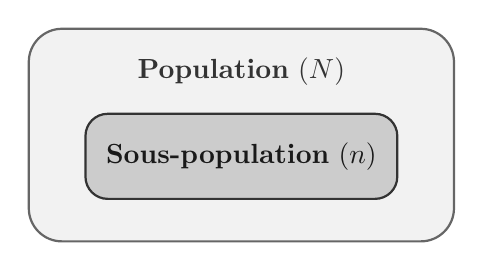
\begin{tikzpicture}[x=9mm,y=9mm]
				\draw[thick, fill=black!5, draw=black!60, rounded corners=12pt] (0,0) rectangle (6,3);
				\node[black!80] at (3, 2.4) {\textbf{Population} ($N$)};
				\draw[thick, fill=black!20, draw=black!80, rounded corners=8pt] (0.8,0.6) rectangle (5.2,1.8);
				\node[black!90] at (3, 1.2) {\textbf{Sous-population} ($n$)};
			\end{tikzpicture}
		\end{center}
		\vspace{-10mm}
	\end{wrapstuff}
	Soit $n$ l'effectif d'une sous-population incluse dans une population globale d'effectif $N$.

	La \textbf{proportion} $p$ de cette sous-population au sein de la population totale est donnée par :

	\cmath{p = \dfrac{n}{N}}
\end{df}

\begin{ex}
	\nline
	\begin{wrapstuff}[r,width=5cm]
		\begin{center}
			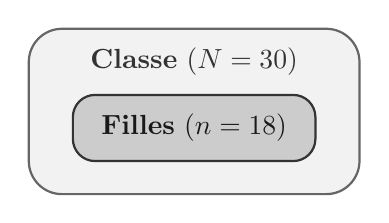
\begin{tikzpicture}[x=7mm,y=7mm]
				\draw[thick, fill=black!5, draw=black!60, rounded corners=12pt] (0,0) rectangle (6,3);
				\node[black!80] at (3, 2.4) {\textbf{Classe} ($N = 30$)};
				\draw[thick, fill=black!20, draw=black!80, rounded corners=8pt] (0.8,0.6) rectangle (5.2,1.8);
				\node[black!90] at (3, 1.2) {\textbf{Filles} ($n = 18$)};
			\end{tikzpicture}
		\end{center}
		\vspace{-15mm}
	\end{wrapstuff}
	Dans une classe de $30$ élèves, il y a $18$ filles.

	La proportion de filles dans cette classe est : $p = \dfrac{18}{30} = 0{,}6$ (soit $60$\%)
\end{ex}

\vspace{8mm}
\begin{prop}
	Une \textbf{proportion} s'exprime par un nombre compris entre $0$ et $1$ (soit entre $0\,\%$ et $100\,\%$). On a : \cmath{0 \leqslant p \leqslant 1}
\end{prop}

\begin{rmq}
	\nline
	\begin{itemize}
		\item La \textbf{proportion} est une valeur théorique ou fixe mesurée sur une population globale.
		\item La \textbf{fréquence} est le résultat d'une observation ou d'un comptage sur un échantillon donné (par exemple lors d'une expérience aléatoire ou d'un sondage).
	\end{itemize}
\end{rmq}

\begin{rmq}
	Pour retrouver les trois formules associées :
	\begin{wrapstuff}[r,width=7cm]
		\vspace{-5mm}
		\begin{center}
			\begin{tikzpicture}[x=8mm,y=8mm]
				% Triangle principal
				\draw[thick] (0,0) -- (3,0) -- (1.5,2.5) -- cycle;
				\draw[thick] (0,1.1) -- (3,1.1);
				\draw[thick] (1.5,0) -- (1.5,1.1);
				% Labels
				\node at (1.5, 1.6) {\textbf{$n$}};
				\node at (0.75, 0.55) {\textbf{$p$}};
				\node at (2.25, 0.55) {\textbf{$N$}};
				\node at (1.5, 0.55) {\Huge$\times$};
			\end{tikzpicture}
		\end{center}
		\vspace{-10mm}
	\end{wrapstuff}
	\begin{itemize}
		\item \makebox[2cm][l]{$p = \dfrac{n}{N}$} pour calculer une proportion
		\item \makebox[2cm][l]{$n = p \times N$} pour calculer un effectif partiel
		\item \makebox[2cm][l]{$N = \dfrac{n}{p}$} pour retrouver l'effectif total
	\end{itemize}
\end{rmq}

\begin{ex}
	\nline
	\begin{enumerate}
		\item \textbf{Calculer une proportion :} Dans une entreprise de $250$ salariés, $65$ travaillent dans le service commercial.

		      \[
			      p = \dfrac{n}{N} = \dfrac{65}{250} = 0{,}26 \quad \text{soit } 26\,\%
		      \]

		      La proportion de salariés travaillant au service commercial est de $26\,\%$.

		\item \textbf{Calculer un effectif :} Dans un lycée de $1\,200$ élèves, $15\,\%$ des élèves sont inscrits en spécialité Mathématiques (soit $p = 0{,}15$).

		      \[
			      {n = p \times N = 0{,}15 \times 1\,200 = 180}
		      \]

		      Il y a $180$ élèves inscrits en spécialité Mathématiques.

		\item \textbf{Retrouver l'effectif total :} Dans un club sportif, $42$ adhérents jouent au tennis, ce qui représente $35\,\%$ de l'effectif du club ($p = 0{,}35$).

		      \[
			      N = \dfrac{n}{p} = \dfrac{42}{0{,}35} = 120
		      \]

		      Le club compte $120$ adhérents au total.
	\end{enumerate}
\end{ex}

\subsection{Proportion de proportion}

\begin{prop}
	\nline
	\begin{wrapstuff}[r,width=7.5cm]
		\begin{center}
			\begin{tikzpicture}[x=1cm,y=1cm]
				\draw[thick, fill=gray!5, draw=gray!60, rounded corners=12pt] (0,0) rectangle (7,4.5);
				\node[gray!80!black, font=\small] at (1.8, 4.1) {\textbf{Population} $E$};
				\draw[thick, fill=black!10, draw=black!60, rounded corners=10pt] (0.6,0.5) rectangle (5.2,3.4);
				\node[black!80!black, font=\small] at (2.1, 3) {\textbf{Population} $B$};
				\draw[thick, fill=black!30, draw=black!90!black, rounded corners=8pt] (1.1,0.9) rectangle (3.5,2.4);
				\node[black!90!black, font=\small] at (2.3, 1.65) {\textbf{Sous-pop.} $A$};
				\draw[->, >=Stealth, thick, black!80!black] (3.6, 1.65) -- (4.8, 1.65) node[midway, above, font=\footnotesize] {$p_1$};
				\draw[->, >=Stealth, thick, gray!80!black] (5.3, 2) -- (6.4, 2) node[midway, above, font=\footnotesize] {$p_2$};
			\end{tikzpicture}
			\vspace{-23mm}
		\end{center}
	\end{wrapstuff}

	Soit une sous-population $A$ incluse dans $B$, elle-même incluse dans une population $E$.

	Si $A$ a une proportion $p_1$ dans $B$, et $B$ a une proportion $p_2$ dans $E$, alors la proportion $p$ de $A$ dans $E$ est :

	\cmath{p = p_1 \times p_2}

\end{prop}

\vspace{12mm}

\begin{ex}
	Dans un lycée, $60\,\%$ des élèves sont en classe de Seconde (soit $p_1 = 0{,}6$).

	Parmi ces élèves de Seconde, $55\,\%$ étudient l'espagnol en LV2 (soit $p_2 = 0{,}55$).

	La proportion $p$ d'élèves de Seconde qui étudient l'espagnol dans l'ensemble du lycée est :

	\cmath{p = p_1 \times p_2 = 0{,}6 \times 0{,}55 = 0{,}33 \quad \text{(soit } 33\,\%\text{)}}

	Ainsi, $33\,\%$ des élèves du lycée sont des élèves de Seconde qui étudient l'espagnol.
\end{ex}

\begin{rmq}
	Prendre une proportion d'une autre proportion revient à les \textbf{multiplier entre elles}.

	Par exemple, calculer $50\,\%$ de $30\,\%$ revient à effectuer : $\quad 0{,}5 \times 0{,}3 = 0{,}15 \quad \text{(soit } 15\,\%\text{)}$
\end{rmq}

\section{Évolution et taux d'évolution}

\subsection{Taux d'évolution}

\begin{df}
	\nline
	\begin{wrapstuff}[r,width=6cm]
		\begin{center}
			\begin{tikzpicture}[x=1cm,y=1cm,>=Stealth]
				\node[ draw=black!80, fill=black!5, thick, rounded corners=4pt, inner sep=8pt, align=center ] (T) at (2.5,0) {Taux d'évolution\\$\pm t\,\%$};
				\node (VI) at (0,0) {$V_I$};
				\node (VF) at (5,0) {$V_F$};
				\draw[->, thick] (VI) -- (T);
				\draw[->, thick] (T) -- (VF);
			\end{tikzpicture}
		\end{center}
	\end{wrapstuff}
	Soit une grandeur passant d'une \textbf{valeur initiale} $V_I$ à une \textbf{valeur finale} $V_F$ (avec $V_I > 0$).

	Le \textbf{taux d'évolution} (ou variation relative) $t$ est donné par :

	\cmath{t = \dfrac{V_F - V_I}{V_I}}

	Pour l'exprimer en \textbf{pourcentage}, on calcule :
	\cmath{t_{\,\%} = \dfrac{V_F - V_I}{V_I} \times 100}
\end{df}

\begin{ex}
	\nline
	\begin{wrapstuff}[r,width=6cm]
		\begin{center}
			\begin{tikzpicture}[x=1cm,y=1cm,>=Stealth]
				\node[ draw=black!80, fill=black!5, thick, rounded corners=4pt, inner sep=8pt, align=center ] (T) at (2,0) {$+30\,\%$};
				\node (VI) at (0,0) {$9{,}50\eur{}$};
				\node (VF) at (4,0) {$12{,}35\eur{}$};
				\draw[->, thick] (VI) -- (T);
				\draw[->, thick] (T) -- (VF);
			\end{tikzpicture}
		\end{center}
		% \vspace{-8mm}
	\end{wrapstuff}
	Le prix d'un livre passe de $V_I = 9{,}50$\eur{} à $V_F = 12{,}35$\eur{}.

	Le taux d'évolution est :

	\cmath{t = \dfrac{12{,}35 - 9{,}50}{9{,}50} = \dfrac{2{,}85}{9{,}50} = 0{,}30}

	Le prix a donc augmenté de $30\,\%$.
\end{ex}

\begin{rmq}
	\nline
	\begin{itemize}
		\item Si le taux d'évolution $t$ est positif ($t > 0$), il s'agit d'une \textbf{augmentation}.
		\item Si le taux d'évolution $t$ est négatif ($t < 0$), il s'agit d'une \textbf{diminution}.
	\end{itemize}
\end{rmq}

\subsection{Coefficient multiplicateur}

\begin{prop}
	Augmenter ou diminuer une valeur initiale $V_I$ d'un taux de $t_{\,\%}$ revient à la multiplier par $\pa{1 + \dfrac{t}{100}}$.

	La valeur finale est alors donnée par :

	\[
		V_F = V_I \times \left( 1 + \frac{t}{100} \right)
	\]

	Le nombre $CM = \pa{1 + \dfrac{t}{100}}$ est appelé le \textbf{coefficient multiplicateur}.
	\begin{center}
		\begin{tikzpicture}[x=1cm,y=1cm,>=Stealth]
			\node[ draw=black!80, fill=black!5, thick, rounded corners=4pt, inner sep=8pt, align=center ] (T) at (3,0) {$\pm t\,\%$};
			\node (VI) at (0,0) {$V_I$};
			\node (VF) at (6,0) {$V_F$};
			\draw[->, thick] (VI) -- (T);
			\draw[->, thick] (T) -- (VF);
			\draw[->, thick, shorten >=3mm, shorten <=3mm] (VI.south) to[out=-30, in=-150] node[below=1mm] {$\times\,CM$} (VF.south);
		\end{tikzpicture}
	\end{center}
\end{prop}

\begin{demo}
	Appliquer une variation de $t\,\%$ à une valeur initiale $V_I$ consiste à ajouter (ou retrancher si $t < 0$) la partie correspondante :

	\[
		V_F = V_I + \frac{t}{100} \times V_I
	\]

	En factorisant par $V_I$, on obtient :

	\[
		V_F = V_I \times \left( 1 + \frac{t}{100} \right)
	\]
\end{demo}

\begin{ex}
	Un article coûtant $80$\eur{} subit une hausse de $15\,\%$ (soit $t = +15$).
	\begin{wrapstuff}[r,width=6cm]
		\begin{center}
			\begin{tikzpicture}[x=0.75cm,y=1cm,>=Stealth]
				\node[ draw=black!80, fill=black!5, thick, rounded corners=4pt, inner sep=6pt, align=center ] (T) at (2.5,0) {$+15\,\%$};
				\node (VI) at (0,0) {$80\text{\eur{}}$};
				\node (VF) at (5,0) {$92\text{\eur{}}$};
				\draw[->, thick] (VI) -- (T);
				\draw[->, thick] (T) -- (VF);
				\draw[->, thick, shorten >=3mm, shorten <=3mm] (VI.south) to[out=-30, in=-150] node[below=1mm] {$\times\,1{,}15$} (VF.south);
			\end{tikzpicture}
		\end{center}
		\vspace{-10mm}
	\end{wrapstuff}

	Le coefficient multiplicateur associé est :

	\cmath{CM = 1 + \dfrac{15}{100} = 1 + 0{,}15 = 1{,}15}

	Le nouveau prix $V_F$ est donc : $\quad V_F = 80 \times 1{,}15 = 92\text{\eur{}}$
\end{ex}

\begin{rmq}
	Pour une grandeur passant d'une valeur initiale $V_I$ à une valeur finale $V_F$ avec un taux d'évolution $t$ exprimé en pourcentage ($t_{\,\%}$) et un coefficient multiplicateur $CM$ :

	\begin{itemize}
		\item \makebox[4cm][l]{$t = \dfrac{V_F - V_I}{V_I} \times 100$}
		      pour calculer le taux d'évolution en pourcentage
		\item \makebox[4cm][l]{$CM = 1 + \dfrac{t}{100}$} pour obtenir le coefficient multiplicateur à partir du taux $t\,\%$
		\item \makebox[4cm][l]{$t = (CM - 1) \times 100$} pour retrouver le taux en pourcentage à partir du $CM$
	\end{itemize}

	Pour passer facilement du taux d'évolution $t\,\%$ au coefficient multiplicateur $CM$ (et inversement), on peut utiliser le petit schéma ci-dessous :

	\begin{center}
		\begin{tikzpicture}[x=1cm,y=1cm,>=Stealth]
			\node[font=\large] (T) at (0,0) {$t$};
			\node[font=\large] (M) at (3,0) {};
			\node[font=\large] (CM) at (6.5,0) {$CM$};
			\draw[->, thick,shorten >=1mm, shorten <=1mm] ([yshift=1mm]T.east) -- node[above] {$\div\,100$} ([yshift=1mm]M.west);
			\draw[->, thick,shorten >=1mm, shorten <=1mm] ([yshift=1mm]M.east) -- node[above] {$+1$} ([yshift=1mm]CM.west);

			% Trajet retour (vers la gauche, decale vers le bas)
			\draw[->, thick, shorten >=1mm, shorten <=1mm] ([yshift=-1mm]CM.west) -- node[below] {$-1$} ([yshift=-1mm]M.east);
			\draw[->, thick, shorten >=1mm, shorten <=1mm] ([yshift=-1mm]M.west) -- node[below] {$\times\,100$} ([yshift=-1mm]T.east);
		\end{tikzpicture}
	\end{center}
\end{rmq}

\begin{exercice}
	Le prix d'un smartphone est initialement de $320$\eur{}. Lors d'une vente flash, ce prix subit une baisse de $15\,\%$.

	Calculer le prix final de ce smartphone après la réduction.

	\begin{correction}
		Calculons le coefficient multiplicateur correspondant à une baisse de $15\,\%$ :

		\cmath{CM = 1 + \dfrac{-15}{100} = 1 - 0{,}15 = 0{,}85}

		Calculons la valeur finale $V_F$ :

		\cmath{V_F = V_I \times CM = 320 \times 0{,}85 = 272\text{\eur{}}}

		Le prix du smartphone après réduction est donc de $272$\eur{}.
	\end{correction}
\end{exercice}

\begin{exercice}
	Après une augmentation de $8\,\%$, le loyer mensuel d'un appartement s'élève désormais à $648$\eur{}.

	Déterminer le montant du loyer avant cette augmentation.

	\begin{correction}
		Le coefficient multiplicateur associé à une hausse de $8\,\%$ est :

		\cmath{CM = 1 + \dfrac{8}{100} = 1{,}08}

		On cherche la valeur initiale $V_I$ telle que $V_F = V_I \times CM$, c'est-à-dire :

		\cmath{648 = V_I \times 1{,}08}

		D'où :

		\cmath{V_I = \dfrac{648}{1{,}08} = 600\text{\eur{}}}

		Le loyer avant augmentation était de $600$\eur{}.
	\end{correction}
\end{exercice}

\begin{exercice}
	Une étude statistique montre qu'entre deux années consécutives, le nombre de clients d'un magasin a été multiplié par un coefficient $CM = 0{,}82$.

	Déterminer le taux d'évolution exprimé en pourcentage du nombre de clients.

	\begin{correction}
		On utilise la formule reliant le coefficient multiplicateur et le taux en pourcentage :

		\cmath{t_{\,\%} = (CM - 1) \times 100}

		En remplaçant par la valeur du $CM$ :

		\cmath{t_{\,\%} = (0{,}82 - 1) \times 100 = -0{,}18 \times 100 = -18\,\%}

		Le nombre de clients a donc subi une diminution de $18\,\%$.
	\end{correction}
\end{exercice}

\section{Évolutions successives et évolution réciproque}

\subsection{Évolutions successives}

\begin{prop}
	Lorsqu'une grandeur subit $n$ évolutions successives de coefficients multiplicateurs respectifs $CM_1$, $CM_2$, $\dots$, $CM_n$, le \textbf{coefficient multiplicateur global} $CM_g$ est égal au produit de tous les coefficients multiplicateurs :

	\[
		CM_g = CM_1 \times CM_2 \times \dots \times CM_n
	\]

	La valeur finale $V_F$ après ces $n$ évolutions s'obtient alors directement par : \quad $V_F = V_I \times CM_g$

	\begin{center}
		\begin{tikzpicture}[x=1cm,y=1cm,>=Stealth]
			\node (V0) at (0,0) {$V_0$};
			\node (V1) at (3.2,0) {$V_1$};
			\node (V2) at (6.4,0) {$V_2$};
			\node (Vn1) at (8.0,0) {$\phantom{I}\ldots\phantom{I}$};
			\node (Vn) at (11.2,0) {$V_n$};
			\node[ draw=black!80, fill=black!5, thick, rounded corners=4pt, inner sep=5pt, align=center ] (T1) at (1.6,0) {$t_1\,\%$};
			\node[ draw=black!80, fill=black!5, thick, rounded corners=4pt, inner sep=5pt, align=center ] (T2) at (4.8,0) {$t_2\,\%$};
			\node[ draw=black!80, fill=black!5, thick, rounded corners=4pt, inner sep=5pt, align=center ] (Tn) at (9.6,0) {$t_n\,\%$};
			\draw[->, thick] (V0) -- (T1);
			\draw[->, thick] (T1) -- (V1);
			\draw[->, thick] (V1) -- (T2);
			\draw[->, thick] (T2) -- (V2);
			\draw[->, thick, looseness=0] (V2) -- (Vn1);
			\draw[->, thick] (Vn1) -- (Tn);
			\draw[->, thick] (Tn) -- (Vn);
			\draw[->, thick, shorten >=2mm, shorten <=2mm] (V0.north) to[out=35, in=145] node[above=1mm] {$\times\,CM_1$} (V1.north);
			\draw[->, thick, shorten >=2mm, shorten <=2mm] (V1.north) to[out=35, in=145] node[above=1mm] {$\times\,CM_2$} (V2.north);
			\draw[->, thick, shorten >=2mm, shorten <=2mm] (Vn1.north) to[out=35, in=145] node[above=1mm] {$\times\,CM_n$} (Vn.north);
			\draw[->, thick, dashed, shorten <=2mm] (V2.north) to[out=35, in=180] ++(1,0.45);
			\draw[->, thick, shorten >=3mm, shorten <=3mm] (V0.south) to[out=-45, in=-135, looseness=0.35] node[below=1.5mm] {$\times\,CM_g = \times\,(CM_1 \times CM_2 \times \dots \times CM_n)$} (Vn.south);
		\end{tikzpicture}
	\end{center}
\end{prop}

\begin{ex}
	Le prix d'un vêtement de $50$\eur{} augmente d'abord de $10\,\%$, puis baisse de $20\,\%$, et augmente de $5\,\%$.
	\begin{multicols}{3}
		\begin{itemize}
			\item $CM_1 = 1 + \dfrac{10}{100} = 1{,}10$
			\item $CM_2 = 1 - \dfrac{20}{100} = 0{,}80$
			\item $CM_3 = 1 + \dfrac{5}{100} = 1{,}05$
		\end{itemize}
	\end{multicols}

	Le coefficient multiplicateur global est :

	\cmath{CM_g = CM_1 \times CM_2 \times CM_3 = 1{,}10 \times 0{,}80 \times 1{,}05 = 0{,}924}

	Le prix final du vêtement est :

	\cmath{V_F = 50 \times 0{,}924 = 46{,}20\text{\eur{}}}

	Le taux d'évolution global est :

	\cmath{t_g = (CM_g - 1) \times 100 = (0{,}924 - 1) \times 100 = -7{,}6\,\%}

	Soit une baisse globale de $7{,}6\,\%$.
\end{ex}

\begin{erreur}
	On ne peut pas additionner ni soustraire directement les pourcentages d'évolutions successives !

	Par exemple, une hausse de $20\,\%$ suivie d'une baisse de $20\,\%$ \textbf{ne correspond pas} à une variation nulle ($0\,\%$).

	En effet :
	\begin{multicols}{2}
		\begin{itemize}
			\item Hausse de $20\,\%$ : \quad $CM_1 = 1 + \dfrac{20}{100} = 1{,}20$
			\item Baisse de $20\,\%$ : \quad $CM_2 = 1 - \dfrac{20}{100} = 0{,}80$
		\end{itemize}
	\end{multicols}

	On a : \cmath{CM_g = 1{,}20 \times 0{,}80 = 0{,}96}

	Le taux global est : \cmath{t_g = (0{,}96 - 1) \times 100 = -4\,\%}

	L'évolution globale est donc une \textbf{baisse de $4\,\%$}.

	Pour compenser exactement une hausse de $20\,\%$ et revenir à la valeur initiale, la baisse réciproque doit être différente de $20\,\%$.
\end{erreur}

\subsection{Évolution réciproque}

\begin{defn}
	\nline
	\begin{wrapstuff}[r, width=7cm]
		\begin{center}
			\vspace{5mm}
			\begin{tikzpicture}[x=1cm,y=1cm,>=Stealth]
				\node (VI1) at (0,0) {$V_I$};
				\node (VF) at (2.8,0) {$V_F$};
				\node (VI2) at (5.6,0) {$V_I$};
				\node[ draw=black!80, fill=black!5, thick, rounded corners=4pt, inner sep=5pt, minimum width=1cm, align=center ] (T) at (1.4,0) {$t$};
				\node[ draw=black!80, fill=black!5, thick, rounded corners=4pt, inner sep=5pt, minimum width=1cm, align=center ] (TR) at (4.2,0) {$t_R$};
				\draw[->, thick] (VI1) -- (T);
				\draw[->, thick] (T) -- (VF);
				\draw[->, thick] (VF) -- (TR);
				\draw[->, thick] (TR) -- (VI2);
			\end{tikzpicture}
			\vspace{1mm}
		\end{center}
	\end{wrapstuff}

	On considère une grandeur subissant une évolution d'une valeur initiale $V_I$ vers une valeur finale $V_F$.

	L'\textbf{évolution réciproque} est l'évolution qui permet de revenir de la valeur finale $V_F$ à la valeur initiale $V_I$.

	Elle compense exactement la variation subie lors de l'évolution initiale.

	Son taux d'évolution est appelé \textbf{taux d'évolution réciproque}, noté $t_R$.
\end{defn}

\begin{prop}
	\nline
	\begin{wrapstuff}[r, width=7cm]
		\begin{center}
			\vspace{5mm}
			\begin{tikzpicture}[x=1cm,y=1cm,>=Stealth]
				% Nœuds des valeurs
				\node (VI1) at (0,0) {$V_I$};
				\node (VF) at (2.8,0) {$V_F$};
				\node (VI2) at (5.6,0) {$V_I$};

				% Boîtes de taux
				\node[ draw=black!80, fill=black!5, thick, rounded corners=4pt, inner sep=5pt, minimum width=1cm, align=center ] (T) at (1.4,0) {$t$};
				\node[ draw=black!80, fill=black!5, thick, rounded corners=4pt, inner sep=5pt, minimum width=1cm, align=center ] (TR) at (4.2,0) {$t_R$};

				% Flèches horizontales
				\draw[->, thick] (VI1) -- (T);
				\draw[->, thick] (T) -- (VF);
				\draw[->, thick] (VF) -- (TR);
				\draw[->, thick] (TR) -- (VI2);

				% Arcs sous les boîtes (CM et CMR)
				\draw[->, thick, shorten >=2mm, shorten <=2mm] (VI1.south) to[out=-35, in=-145] node[below=1mm, font=\small] {$\times\,CM$} (VF.south);
				\draw[->, thick, shorten >=2mm, shorten <=2mm] (VF.south) to[out=-35, in=-145] node[below=1mm, font=\small] {$\times\,CM_R$} (VI2.south);
			\end{tikzpicture}
		\end{center}
	\end{wrapstuff}

	Soit une évolution de taux $t$ et son coefficient multiplicateur associé $CM$.

	L'évolution réciproque, de taux $t_R$, possède un \textbf{coefficient multiplicateur réciproque}, noté $CM_R$, vérifiant la relation :

	\cmath{CM_R = \dfrac{1}{CM}}

	Le taux d'évolution réciproque s'obtient ensuite par : \qquad $t_R = (CM_R - 1) \times 100$
\end{prop}

\begin{demo}
	Par définition de l'évolution réciproque, le coefficient $CM_R$ permet de revenir de $V_F$ à $V_I$ :

	\[
		\def\arraystretch{1.7} \begin{array}{rrcll}
			     & V_F & = & V_I \times CM                                                                  \\
			\iff & V_I & = & \dfrac{V_F}{CM}          & \text{(on isole } V_I\text{)}                       \\
			\iff & V_I & = & V_F \times \dfrac{1}{CM} & \text{(diviser revient à multiplier par l'inverse)}
		\end{array}
	\]

	Par identification avec la relation $V_I = V_F \times CM_R$, on en déduit immédiatement : \quad $CM_R = \dfrac{1}{CM}$
\end{demo}

\begin{exemple}
	Un article subit une hausse de $20\,\%$. On cherche à déterminer le taux de l'évolution réciproque $t_R$ permettant de revenir au prix initial.

	\begin{enumerate}
		\item {Calcul du coefficient multiplicateur initial :}
		      \[
			      CM = 1 + \frac{20}{100} = 1{,}20
		      \]
		\item {Calcul du coefficient multiplicateur réciproque :}
		      \[
			      CM_R = \frac{1}{CM} = \frac{1}{1{,}20} = \frac{5}{6} \approx 0{,}8333
		      \]
		\item {Calcul du taux d'évolution réciproque :}
		      \[
			      t_R = (CM_R - 1) \times 100 = \left( \frac{5}{6} - 1 \right) \times 100 = -\frac{100}{6} \approx -16{,}67\,\%
		      \]
	\end{enumerate}

	Pour compenser une hausse de $20\,\%$, il faut donc effectuer une baisse d'environ $16{,}67\,\%$.
\end{exemple}

\newpage

\begin{exercice}
	Un laboratoire étudie l'évolution d'une population de \textbf{licornes magiques} dans une forêt enchantée sur trois années consécutives.

	\begin{itemize}
		\item La $1\iere$ année, suite à une surconsommation d'arcs-en-ciel, la population \textbf{augmente de $25\,\%$}.
		\item La $2\ieme$ année, en raison d'une pénurie de paillettes, la population \textbf{chute de $40\,\%$}.
		\item La $3\ieme$ année, grâce à une récolte exceptionnelle d'herbe dorée, la population \textbf{augmente de $50\,\%$}.
	\end{itemize}

	\begin{enumerate}
		\item Déterminer le coefficient multiplicateur associé à chaque évolution annuelle ($CM_1$, $CM_2$ et $CM_3$).
		\item En déduire le coefficient multiplicateur global $CM_g$ sur ces trois années.
		\item Calculer le taux d'évolution global $t_g$ de la population de licornes sur cette période.\\
		      La population a-t-elle augmenté ou diminué au global ?
		\item Le garde forestier souhaite ramener la population de licornes exactement à son niveau initial.
		      \begin{enumerate}
			      \item Calculer le coefficient multiplicateur réciproque $CM_R$.
			      \item En déduire le taux d'évolution réciproque $t_R$ (arrondi au centième près) à appliquer à la population finale.
		      \end{enumerate}
	\end{enumerate}

	\begin{correction}
		\nline
		\begin{enumerate}
			\item {Coefficients multiplicateurs annuels :}
			      \begin{multicols}{3}
				      \begin{itemize}
					      \item $CM_1 = 1 + \dfrac{25}{100} = 1{,}25$
					      \item $CM_2 = 1 + \dfrac{-40}{100} = 0{,}60$
					      \item $CM_3 = 1 + \dfrac{50}{100} = 1{,}50$
				      \end{itemize}
			      \end{multicols}

			\item {Coefficient multiplicateur global :}
			      \[
				      CM_g = CM_1 \times CM_2 \times CM_3 = 1{,}25 \times 0{,}60 \times 1{,}50 = 1{,}125
			      \]

			\item {Taux d'évolution global :}
			      \[
				      t_g = (CM_g - 1) \times 100 = (1{,}125 - 1) \times 100 = +12{,}5\,\%
			      \]
			      Sur les trois années, la population de licornes a subi une \textbf{hausse globale de $12{,}5\,\%$}.

			\item {Évolution réciproque :}
			      \begin{enumerate}
				      \item {Coefficient multiplicateur réciproque :}
				            \[
					            CM_R = \frac{1}{CM_g} = \frac{1}{1{,}125} = \frac{8}{9} \approx 0{,}8889
				            \]

				      \item {Taux d'évolution réciproque :}
				            \[
					            t_R = (CM_R - 1) \times 100 = \left( \frac{8}{9} - 1 \right) \times 100 = \frac{-100}{9} \approx -11{,}11\,\%
				            \]
				            Pour revenir exactement à la population initiale, il faut appliquer une \textbf{baisse d'environ $11{,}11\,\%$}.
			      \end{enumerate}
		\end{enumerate}
	\end{correction}
\end{exercice}

\newpage
\section{Exercices}
 {\small
  \begin{multicols}{2}
	  \begin{exo}{}
	Sachant que, dans un village, il y a $500$ habitants et que $230$ d'entre eux sont des femmes, quelle est la proportion de femmes dans le village ?

	\vspace*{-2mm}\begin{multicols}{4}
	\begin{enumerate}
		\item $1,17$
		\item $0,54$
		\item $0,46$
		\item $2,17$
	\end{enumerate}
	\end{multicols}\vspace*{-4mm}
\end{exo}

	  \begin{exo}{}
	Après le passage de la tempête Irma en septembre $\np{2017}$, $95\%$ des $\np{21050}$ bâtiments de l'île de Saint-Martin ont été détruits.


	Combien de bâtiments cela représente-t-il ? Arrondir à la dizaine près.
\end{exo}

	  \begin{exo}{}
	La forêt amazonienne s'étend sur $5,5$ millions de $\text{km}^2$ et se situe en Amérique du Sud, continent de $17,84$ millions de $\text{km}^2$.


	Calculer la proportion de la superficie qu'occupe la forêt amazonienne sur ce continent. Arrondir à $0,01$\% près.
\end{exo}

	  \begin{exo}{}
	Pour leurs vacances, Mario et ses amis ont un budget total de $850\eur{}$.

	Ils prévoient $35\%$ de ce budget pour l'hébergement.


	Combien leur coûterait l'hébergement ?
\end{exo}

	  \begin{exo}{}
	$19\%$ des élèves d'un lycée sont externes, ce qui représente $285$ élèves.


	Combien d'élèves y-a t-il dans ce lycée ?
\end{exo}

	  \begin{exo}{}
	En $\np{1998}$, le film \textit{Titanic} avait enregistré $\np{20634793}$ entrées. Cette année-là, $170,1$ millions d'entrées sont enregistrées en France, tous films confondus.


	En $\np{2008}$, le film \textit{Bienvenue chez les Ch'tis} enregistrait $\np{20489303}$ entrées pour $212,7$ millions d'entrées au total cette année-là (\textit{source : Cinemondial.com}).


	Lequel de ces deux films a attiré la plus grande proportion de spectateurs ?
\end{exo}

	  \begin{exo}{}
	Dans une classe de $30$ élèves, $12$ sont internes.

	Dans une autre classe de $25$ élèves, $11$ sont internes.
	\begin{enumerate}
		\item Calculer la proportion d'élèves internes dans chacune des deux classes.
		\item Calculer la proportion d'élèves internes sur l'ensemble des deux classes. Arrondir à $0,01$\% près.
	\end{enumerate}
\end{exo}

	  \vfill~\columnbreak
	  \begin{exo}{}
	Un sachet contient des sucettes et des bonbons qui sont soit au chocolat, soit aux fruits.

	\begin{enumerate}
		\item Recopier et compléter le tableau ci-dessous.
	\end{enumerate}
	\begin{center}
		\def\arraystretch{1.5}
		\begin{tabular}{|c|c|c|c|}
			\hline
			                            & \cellcolor{gray!30}Bonbons & \cellcolor{gray!30}Sucettes & \cellcolor{gray!30}Total \\ \hline
			\cellcolor{gray!30}Chocolat & $8$                        &                             &                          \\ \hline
			\cellcolor{gray!30}Fruits   &                            &                             & $32$                     \\ \hline
			\cellcolor{gray!30}Total    & $20$                       &                             & $60$                     \\ \hline
		\end{tabular}
	\end{center}
	\begin{enumerate}[resume]
		\item Calculer la proportion de sucettes dans le sachet. Arrondir à $0,01$\% près.
		\item Calculer la proportion de bonbons aux fruits.
		\item Calculer la proportion de bonbons parmi les sucreries aux fruits.
	\end{enumerate}
\end{exo}

	  \begin{exo}{}
	Dans une entreprise, $70\%$ des employés possèdent une voiture et $\frac{1}{4}$ de ces voitures sont blanches.


	Quel est le pourcentage d'employés possédant une voiture blanche ?

	\vspace*{-2mm}\begin{multicols}{2}
	\begin{enumerate}
		\item $28\%$
		\item $17,5$\%
		\item $35,7$\%
		\item $25\%$
	\end{enumerate}
	\end{multicols}\vspace*{-2mm}
\end{exo}

	  \begin{exo}{}
	Soit $x$ un nombre réel.

	Quelle proportion est la plus grande ?
	\begin{enumerate}
		\item $50\%$ de $50\%$ de $x$
		\item $75\%$ de $25\%$ de $x$
		\item $25\%$ de $75\%$ de $x$
	\end{enumerate}
\end{exo}

	  \begin{exo}{}
	$50\%$ des foyers français possèdent au moins un animal de compagnie et, pour $20\%$ de ces foyers, il s'agit de chats.
	\begin{enumerate}
		\item Quelle proportion des ménages français possèdent au moins un chat comme animal de compagnie ?
		\item Exprimer le résultat sous forme d'un pourcentage.
	\end{enumerate}
\end{exo}

	  \begin{exo}{}
	Dans une grande entreprise, $38,3$\% des salariés sont des cadres et, parmi eux, $86,5$\% optent fréquemment pour le télétravail.
	\begin{enumerate}
		\item Modéliser la situation à l'aide d'un schéma judicieusement choisi.
		\item Quelle proportion de salariés sont des cadres qui optent pour le télétravail ? Arrondir à $0,1$\% près.
	\end{enumerate}
\end{exo}

	  \vfill~\columnbreak
	  \begin{exo}{}
	Dans un centre de tabacologie, sur $\np{1420}$ personnes interrogées, on constate que $15\%$ fument régulièrement des cigarettes électroniques et que, parmi elles, $69\%$ fument toujours des cigarettes.
	\begin{enumerate}
		\item Calculer la proportion de personnes fumant les deux types de cigarettes.
		\item À combien de personnes cela correspond-il ?
	\end{enumerate}
\end{exo}

	  \begin{exo}{}
	Un smartphone initialement affiché à $385$\eur{} est proposé à $254,10$~\eur{} lors d'une promotion.


	Calculer la variation absolue puis la variation relative (en pourcentage) du prix du smartphone.
\end{exo}

	  \begin{exo}{}
	Dans une petite école de village, il y avait $105$ élèves l'an dernier. Cinq de plus sont prévus à la rentrée.


	Calculer la variation absolue puis la variation relative (arrondie à $0,01$\%) du nombre d'élèves entre ces deux années.
\end{exo}

	  \begin{exo}{}
	Pour chacun des taux d'évolution suivants, déterminer le coefficient multiplicateur associé.
	\begin{enumerate}
		\item \textbf{Augmentation :}
		      \vspace*{-2mm}\begin{multicols}{2}\begin{enumerate}
			      \item de $25\%$
			      \item de $74,5$\%
			      \item de $6\%$
			      \item de $0,04$\%
			      \item de $100\%$
			      \item de $350\%$
		      \end{enumerate}\end{multicols}\vspace*{-2mm}
		\item \textbf{Diminution :}
		      \vspace*{-2mm}\begin{multicols}{2}\begin{enumerate}
			      \item de $45\%$
			      \item de $10,6$\%
			      \item de $3\%$
			      \item de $0,008$\%
			      \item de $87,01$\%
		      \end{enumerate}\end{multicols}\vspace*{-2mm}
	\end{enumerate}
\end{exo}

	  \begin{exo}{}
	Pour chacun des coefficients multiplicateurs suivants, déterminer le taux d'évolution associé.

	\vspace*{-2mm}\begin{multicols}{2}
	\begin{enumerate}
		\item $\text{CM} = 1,63$
		\item $\text{CM} = 1,4759$
		\item $\text{CM} = 1,092$
		\item $\text{CM} = 1,005$
		\item $\text{CM} = 2,45$
		\item $\text{CM} = 0,36$
		\item $\text{CM} = 0,453$
		\item $\text{CM} = 0,9832$
		\item $\text{CM} = 0,07$
	\end{enumerate}\end{multicols}\vspace*{-2mm}
\end{exo}

	  \begin{exo}{}
	Soit $V_D = 48$. Dans chacun des cas suivants, déterminer la valeur d'arrivée $V_A$.
	\begin{enumerate}
		\item Après une hausse de $37\%$.
		\item Après une baisse de $11\%$.
	\end{enumerate}
\end{exo}

	  \begin{exo}{}
	Soit $V_A = 91$. Dans chacun des cas suivants, déterminer la valeur de départ $V_D$, arrondie au dixième près.
	\begin{enumerate}
		\item Après une hausse de $37\%$.
		\item Après une baisse de $11\%$.
	\end{enumerate}
\end{exo}

	  \vfill~\columnbreak
	  \begin{exo}{}
	Ci-dessous sont résumés les tarifs des parkings du mont Saint-Michel en $2016$ et en $\np{2018}$.


	\begin{center}
		\def\arraystretch{1.5}
		\begin{tabular}{|c|c|c|} \hline
			                                       & \cellcolor{gray!30}2016 & \cellcolor{gray!30}2018 \\ \hline
			\cellcolor{gray!30}Véhicule individuel & $11,70$~\eur{}          & $12$\eur{}              \\ \hline
			\cellcolor{gray!30}Camping-car         & $17,20$~\eur{}          & $17,60$~\eur{}          \\ \hline
			\cellcolor{gray!30}Moto                & $4,20$~\eur{}           & $4,40$~\eur{}           \\ \hline
		\end{tabular}
	\end{center}


	Pour quelle catégorie de véhicules l'augmentation tarifaire entre $2016$ et $2018$ est-elle la plus grande en euros ? en pourcentage ?
\end{exo}

	  \begin{exo}{}
	Le prix moyen des appartements anciens dans $7$ villes françaises est donné dans le tableau ci-dessous.
	\begin{center}
		\footnotesize
		\begin{tabular}{|c|c|c|c|c|c|}\hline
			                     & \cellcolor{gray!30}A & \cellcolor{gray!30}B & \cellcolor{gray!30}C & \cellcolor{gray!30}D                                                 & \cellcolor{gray!30}E                                                  \\ \hline
			\cellcolor{gray!30}1 & \textbf{Ville}       & \textbf{2016}        & \textbf{2017}        & \textbf{\begin{tabular}[c]{@{}c@{}}variation\\ absolue\end{tabular}} & \textbf{\begin{tabular}[c]{@{}c@{}}variation\\ relative\end{tabular}} \\ \hline
			\cellcolor{gray!30}2 & Strasbourg           & $\np{3279}$          & $\np{3531}$          &                                                                      &                                                                       \\ \hline
			\cellcolor{gray!30}3 & Bordeaux             & $\np{4155}$          & $\np{4599}$          &                                                                      &                                                                       \\ \hline
			\cellcolor{gray!30}4 & Caen                 & $\np{2307}$          & $\np{2390}$          &                                                                      &                                                                       \\ \hline
			\cellcolor{gray!30}5 & Paris                & $\np{8967}$          & $\np{9559}$          &                                                                      &                                                                       \\ \hline
			\cellcolor{gray!30}6 & Nîmes                & $\np{2124}$          & $\np{2381}$          &                                                                      &                                                                       \\ \hline
			\cellcolor{gray!30}7 & Orléans              & $\np{2158}$          & $\np{2111}$          &                                                                      &                                                                       \\ \hline
			\cellcolor{gray!30}8 & Lyon                 & $\np{4279}$          & $\np{4604}$          &                                                                      &                                                                       \\ \hline
		\end{tabular}
	\end{center}

	Les cellules de la colonne \textbf{E} sont au format pourcentage écrit avec une décimale (\textit{source : baromètre LPI-SeLoger}).
	\begin{enumerate}
		\item Quelles formules peut-on entrer dans les cellules \textbf{D3} et \textbf{E3} pour que, une fois recopiées vers le bas, elles affichent les variations absolue et relative pour chacune des villes ?
		\item Reproduire et compléter le tableau.
		\item Dans laquelle de ces villes le prix connaît-il la plus forte augmentation en euros ? en pourcentage ?
	\end{enumerate}
\end{exo}

	  \begin{exo}{}
	L'espérance de vie en $1970$ était de $71,66$ ans en France et de $70,81$ ans aux États-Unis.

	En $\np{2016}$, elle a augmenté de $14,8$\% en France et de $11,1$\% aux États-Unis.


	Déterminer l'espérance de vie en France et aux États-Unis en $\np{2016}$.
\end{exo}

	  \begin{exo}{}
	Recopier et compléter le tableau ci-dessous.


	\begin{center}
		\def\arraystretch{1.5}
		\begin{tabular}{|c|c|c|c|} \hline
			\rowcolor{gray!30}$V_d$ & $V_a$   & $CM$    & $t$ (en \%)             \\ \hline
			$185$                   &         &         & Augmentation de $20\%$  \\ \hline
			                        & $22,95$ &         & Diminution de $15\%$    \\ \hline
			$\np{1075}$             &         & $1,002$ &                         \\ \hline
			$240$                   & $180$   &         &                         \\ \hline
			                        & $38,01$ & $0,21$  &                         \\ \hline
			$421$                   &         &         & Augmentation de $100\%$ \\ \hline
		\end{tabular}
	\end{center}
\end{exo}

	  \vfill~\columnbreak
	  \begin{exo}{}
	Dans chacun des cas suivants, déterminer le taux d'évolution global, arrondi à $0,01$\% près si nécessaire.
	\begin{enumerate}
		\item Lors d'une augmentation de $45\%$ puis d'une augmentation de $70\%$.
		\item Lors d'une diminution de $13,4$\% puis d'une augmentation de $5,8$\%.
		\item Lors d'une diminution de $28,47$\% puis d'une diminution de $37,61$\%.
	\end{enumerate}
\end{exo}

	  \begin{exo}{}
	Dans chacun des cas suivants, déterminer le taux d'évolution réciproque, arrondi à $0,01$\% près :
	\begin{enumerate}
		\item d'une augmentation de $21\%$.
		\item d'une augmentation de $150\%$.
		\item d'une baisse de $43\%$.
		\item d'une baisse de $4,7$\%.
	\end{enumerate}
\end{exo}

	  \begin{exo}{}
	Le prix hors taxes (HT) d'un DVD est de $16$\eur{}.

	Le prix toutes taxes comprises (TTC) d'un jeu vidéo est de $51$\eur{}.

	Le taux de TVA est de $20\%$ sur ce type d'articles.
	\begin{enumerate}
		\item Déterminer le prix TTC de ce DVD.
		\item Déterminer le prix HT de ce jeu vidéo.
	\end{enumerate}
\end{exo}

	  \begin{exo}{}
	Certaines plantes vertes peuvent voir leur croissance augmenter rapidement.

	Une variété grandit de $60\%$ en $3$ mois puis de $50\%$ les $3$ mois suivants.


	Déterminer le taux de croissance sur $6$ mois de cette variété de plante verte.
\end{exo}

	  \begin{exo}{}
	La population d'une ville de $\np{45304}$ habitants augmente de $5\%$ puis diminue de $10\%$ l'année suivante.
	\begin{enumerate}
		\item Calculer le taux d'évolution global sur les deux années.
		\item Calculer le nombre d'habitants après ces évolutions. Arrondir à l'entier le plus proche.
	\end{enumerate}
\end{exo}

	  \begin{exo}{}
	Le prix d'un baril de pétrole a augmenté de $7,34$\% entre août et septembre, puis a augmenté de $9,78$\% en octobre pour chuter ensuite de $11,46$\% en novembre.


	Déterminer le taux d'évolution global du prix d'un baril de pétrole entre août et novembre.
\end{exo}

	  \vfill~\columnbreak
	  \begin{exo}{}
	Le tableau ci-après donne les taux d'évolution successifs du nombre d'objets connectés dans le monde entre les années $2011$ et $\np{2015}$.
	La cellule \textbf{B6} est au format pourcentage écrit avec une décimale (\textit{source : IDATE DigiWorld, Institut de l'audiovisuel et des télécoms en Europe}).


	\begin{center}
		\def\arraystretch{1.5}
		\begin{tabular}{|c|c|c|c|c|c|}
			\hline
			                     & \cellcolor{gray!30}A & \cellcolor{gray!30}B  & \cellcolor{gray!30}C & \cellcolor{gray!30}D & \cellcolor{gray!30}E \\ \hline
			\cellcolor{gray!30}1 & \textbf{Année}       & 2012                  & 2013                 & 2014                 & 2015                 \\ \hline
			\cellcolor{gray!30}2 & \textbf{Taux}        & $57,89$\%             & $46,67$\%            & $40,91$\%            & $35,48$\%            \\ \hline
			\cellcolor{gray!30}3 & \textbf{C.M.}        &                       &                      &                      &                      \\ \hline
			\cellcolor{gray!30}4 &                      &                       &                      &                      &                      \\ \hline
			\cellcolor{gray!30}5 & $CM_g$               & \multicolumn{4}{l|}{}                                                                      \\ \hline
			\cellcolor{gray!30}6 & $T_g$                & \multicolumn{4}{l|}{}                                                                      \\ \hline
		\end{tabular}
	\end{center}


	\begin{enumerate}
		\item Quelle formule faut-il entrer en \textbf{B3} puis recopier vers la droite pour calculer le coefficient multiplicateur associé aux taux d'évolution du dessus ?
		\item Quelles formules faut-il entrer en \textbf{B5} et \textbf{B6} pour calculer le coefficient multiplicateur global et le taux d'évolution global ?
		\item Recopier et compléter le tableau.
	\end{enumerate}
\end{exo}

	  \begin{exo}{}
	Le programme ci-dessous, écrit en Python, permet de calculer le taux d'évolution global, connaissant les deux taux d'évolutions successives $p_1$ et $p_2$.


	\begin{lstlisting}
def Taux_global(p1, p2):
    CM1 = 1+p1/100
    CM2 = 1+p2/100
    CM = .....
    p = .....
    return(p)

print(Taux_global(24,-35))
		\end{lstlisting}


	\begin{enumerate}
		\item Expliquer pourquoi, dans les lignes $2$ et 3, on divise $p_1$ et $p_2$ par $100$.
		\item Recopier et compléter les lignes $4$ et $5$.
		\item Tester ce programme avec $p_1 = 24$ et $p_2 = -35$.
	\end{enumerate}
\end{exo}

	  \begin{exo}{}
	Suite à son passage en machine à laver, un pull a rétréci de $7\%$.


	En utilisant des astuces pour récupérer sa taille d'origine, de quel pourcentage (à $0,1$\% près) doit-il alors s'agrandir ?
\end{exo}

	  \vfill~\columnbreak
	  \begin{exo}{}
	Lorsqu'il va chez son cardiologue, M. Charrier paye sa consultation.

	$70\%$ de ce montant lui est remboursé par la Sécurité sociale. Sur le montant restant à sa charge après remboursement de la Sécurité sociale, sa mutuelle lui rembourse $80\%$.

	Il lui reste finalement $6$\eur{} à sa charge.
	\begin{enumerate}
		\item Quel pourcentage du prix de la consultation sa mutuelle lui rembourse-t-elle ?
		\item Quel pourcentage du prix de la consultation a-t-il finalement payé ?
		\item Quel était le montant de sa consultation au départ ?
	\end{enumerate}
\end{exo}

	  \begin{exo}{}
	L'écharpe de Pierre de forme rectangulaire a rétréci au lavage : sa longueur a diminué de $15\%$ et sa largeur de $20\%$. Son aire est maintenant de $\np{2448}$~$\text{cm}^2$.


	Quelle était son aire avant le lavage ?
\end{exo}

	  \begin{exo}{}
	Dans une ville, un organisme étudie l'évolution de la population. Compte tenu des naissances et des décès, on a constaté que la population a un taux d'accroissement naturel et annuel de $14$ pour mille ($14$\textperthousand).

	En $\np{2015}$, cette ville comptait $\np{120740}$ habitants.

	Si le taux d'accroissement reste le même, à combien peut-on estimer la population de cette ville en $2030$ ?
\end{exo}

	  \vfill~\columnbreak
	  \vfill~
  \end{multicols}
 }

\chapter{Statistiques descriptives}

\section{Vocabulaire et présentation d'une série}

\begin{defin}[Vocabulaire de base]
	\textbf{Population et individu :} L'ensemble étudié en statistiques est appelé la \textbf{population}. Chaque élément qui constitue cet ensemble est un \textbf{individu}.

	\textbf{Caractère :} C'est la propriété ou la grandeur étudiée sur chaque individu.
	\begin{itemize}
		\item Un caractère est dit \textbf{qualitatif} lorsque ses valeurs (appelées modalités) ne sont pas des nombres (ex. : couleur des yeux, filière).
		\item Un caractère est dit \textbf{quantitatif} lorsqu'il prend des valeurs numériques.
		      \begin{itemize}
			      \item Il est \textbf{discret} si les valeurs sont \og{}isolées\fg{} (ex. : nombre d'enfants)
			      \item Il est \textbf{continu} si les valeurs sont regroupées en intervalles appelés \textbf{classes} (ex. : taille en $\text{cm}$)
		      \end{itemize}
	\end{itemize}
\end{defin}

\begin{defin}[Effectifs, fréquences et cumul]
	Soit une série statistique de $k$ valeurs distinctes $x_1, x_2, \dots, x_k$ (ordonnées dans l'ordre croissant).
	\begin{itemize}
		\item L'\textbf{effectif} $n_i$ associé à la valeur $x_i$ est le nombre d'individus possédant cette valeur.
		\item L'\textbf{effectif total} est la somme de tous les effectifs :
		      \[
			      N = n_1 + n_2 + \dots + n_k \qquad = \displaystyle\sum_{i=1}^k n_i
		      \]
		\item La \textbf{fréquence} $f_i$ associée à la valeur $x_i$ est le quotient $f_i = \dfrac{n_i}{N}$. La somme des fréquences est égale à $1$ (ou $100\,\%$).
		\item L'\textbf{effectif cumulé croissant (E.C.C.)} associé à la valeur $x_i$ est la somme des effectifs de toutes les valeurs inférieures ou égales à $x_i$.
		\item La \textbf{fréquence cumulée croissante (F.C.C.)} associée à la valeur $x_i$ est la somme des fréquences de toutes les valeurs inférieures ou égales à $x_i$.
	\end{itemize}
\end{defin}

\begin{ex}[Présentation des données sous forme de tableau]
	Voici une série de notes obtenues par un groupe d'élèves :

	\[
		4 \ ; \ 6 \ ; \ 7 \ ; \ 12 \ ; \ 12 \ ; \ 17 \ ; \ 18 \ ; \ 18
	\]

	L'effectif total est $N = 8$.

	\begin{center}
		\rnc{\arraystretch}{1.5}
		\begin{tabular}{|r|c|c|c|c|c|c|}
			\hline
			\rowcolor{gray!30}Notes $x_i$          & 4              & 6              & 7              & 12             & 17             & 18             \\ \hline
			Effectifs $n_i$                        & 1              & 1              & 1              & 2              & 1              & 2              \\ \hline
			E.C.C.                                 & 1              & 2              & 3              & 5              & 6              & 8              \\ \hline
			\rule[-4mm]{0mm}{11mm}Fréquences $f_i$ & $\dfrac{1}{8}$ & $\dfrac{1}{8}$ & $\dfrac{1}{8}$ & $\dfrac{2}{8}$ & $\dfrac{1}{8}$ & $\dfrac{2}{8}$ \\ \hline
			\rule[-4mm]{0mm}{11mm}F.C.C.           & $\dfrac{1}{8}$ & $\dfrac{2}{8}$ & $\dfrac{3}{8}$ & $\dfrac{5}{8}$ & $\dfrac{6}{8}$ & $\dfrac{8}{8}$ \\ \hline
		\end{tabular}
	\end{center}
\end{ex}

\section{Caractéristiques de position}

Les caractéristiques de position (ou de tendance centrale) résument une série statistique par une valeur numérique représentative.

\subsection{Moyenne}

\begin{defin}[Moyenne pondérée]
	La \textbf{moyenne} d'une série statistique de valeurs $x_1, x_2, \dots, x_k$ affectées des effectifs $n_1, n_2, \dots, n_k$ est notée $\bar{x}$. Elle est définie par :

	\[
		\bar{x} = \dfrac{n_1 x_1 + n_2 x_2 + \dots + n_k x_k}{N} \qquad = \dfrac{1}{N} \sum_{i=1}^k n_i x_i
	\]

	Dans le cas d'un caractère continu regroupé en classes $[a ; b[$, on effectue le calcul en remplaçant chaque classe par son centre $\dfrac{a+b}{2}$.
\end{defin}

\begin{ex}[Calcul d'une moyenne simple et pondérée]
	On étudie le nombre de frères et sœurs des $21$ élèves d'une classe de 1STMG :
	\[
		0 \ ; \ 0 \ ; \ 0 \ ; \ 0 \ ; \ 0 \ ; \ 1 \ ; \ 1 \ ; \ 1 \ ; \ 1 \ ; \ 1 \ ; \ 1 \ ; \ 1 \ ; \ 1 \ ; \ 2 \ ; \ 2 \ ; \ 2 \ ; \ 2 \ ; \ 3 \ ; \ 3 \ ; \ 3 \ ; \ 4
	\]

	\begin{enumerate}
		\item \textbf{Calcul non pondéré (moyenne simple) :}

		      On additionne directement l'ensemble des $21$ valeurs individuelles :
		      \[
			      \bar{x} = \dfrac{0 + 0 + 0 + 0 + 0 + 1 + 1 + 1 + 1 + 1 + 1 + 1 + 1 + 2 + 2 + 2 + 2 + 3 + 3 + 3 + 4}{21} = \dfrac{29}{21} \approx 1{,}38
		      \]

		\item \textbf{Calcul pondéré (à partir du tableau d'effectifs) :}

		      En regroupant les valeurs identiques avec leur effectif $n_i$ associé :
		      \begin{center}
			      \rnc{\arraystretch}{1.3}
			      \begin{tabular}{|r|c|c|c|c|c|} \hline
				      \rowcolor{gray!30} Nombre de frères et sœurs $x_i$ & 0 & 1 & 2 & 3 & 4 \\ \hline
				      Effectifs $n_i$                                    & 5 & 8 & 4 & 3 & 1 \\ \hline
			      \end{tabular}
		      \end{center}

		      Le calcul devient :
		      \[
			      \bar{x} = \dfrac{5 \times 0 + 8 \times 1 + 4 \times 2 + 3 \times 3 + 1 \times 4}{21} = \dfrac{29}{21} \approx 1{,}38
		      \]
	\end{enumerate}

	On vérifie bien que les deux méthodes mènent au même résultat.
\end{ex}

\begin{ex}[Calcul de la moyenne d'un caractère continu]
	Dans une classe de 1STMG, on mesure la taille des élèves (en $\text{cm}$) regroupée par classes d'amplitude $5\text{ cm}$ :

	\begin{center}
		\rnc{\arraystretch}{1.3}
		\begin{tabular}{|c|c|c|c|}\hline
			\rowcolor{gray!30}
			Taille $I_i$ (en $\text{cm}$) & Centre $c_i$ & Effectif $n_i$ & $n_i \times c_i$              \\ \hline
			$[160 ; 165[$                 & $162{,}5$    & 4              & $4 \times 162{,}5 = 650$      \\ \hline
			$[165 ; 170[$                 & $167{,}5$    & 9              & $9 \times 167{,}5 = 1507{,}5$ \\ \hline
			$[170 ; 175[$                 & $172{,}5$    & 8              & $8 \times 172{,}5 = 1380$     \\ \hline
			$[175 ; 180[$                 & $177{,}5$    & 3              & $3 \times 177{,}5 = 532{,}5$  \\ \hline
			\textbf{Total}                & -            & $N = 24$       & $4070$                        \\ \hline
		\end{tabular}
	\end{center}

	On calcule la taille moyenne estimée en appliquant la formule de la moyenne pondérée aux centres des classes :
	\[
		\bar{x} = \dfrac{4 \times 162{,}5 + 9 \times 167{,}5 + 8 \times 172{,}5 + 3 \times 177{,}5}{24} = \dfrac{4070}{24} \approx 169{,}58\text{ cm}
	\]
\end{ex}

\newpage

\begin{prop}[Linéarité de la moyenne]
	Soit une série de moyenne $\bar{x}$ et deux réels $a$ et $b$.
	\begin{itemize}
		\item Si on multiplie toutes les valeurs de la série par $a$, la nouvelle moyenne devient $a\bar{x}$.
		\item Si on ajoute $b$ à toutes les valeurs de la série, la nouvelle moyenne devient $\bar{x} + b$.
		\item De façon générale, les valeurs $a x_i + b$ ont pour moyenne $a\bar{x} + b$.
	\end{itemize}
\end{prop}

\begin{methode}[Utiliser la linéarité de la moyenne]
	Un relevé du prix au litre d'essence dans 5 stations donne :
	\[
		1{,}50\text{ \euro}, 1{,}44\text{ \euro}, 1{,}51\text{ \euro}, 1{,}62\text{ \euro} \text{ et } 1{,}58\text{ \euro}
	\]

	\begin{enumerate}
		\item Calculer le prix moyen initial.
		\item Calculer le prix moyen après une augmentation générale de $30\,\%$.
		\item Calculer le prix moyen final après une remise de $0{,}15\text{ \euro}$ par litre.
	\end{enumerate}

	\begin{correction}
		\nline
		\begin{enumerate}
			\item Prix moyen initial : $\bar{x} = \dfrac{1{,}50 + 1{,}44 + 1{,}51 + 1{,}62 + 1{,}58}{5} = \dfrac{7{,}65}{5} = 1{,}53\text{ \euro}$.
			\item Augmenter de $30\,\%$ revient à multiplier par $1{,}30$. Par linéarité :
			      \[
				      \bar{x}_{\text{hausse}} = 1{,}53 \times 1{,}30 = 1{,}989\text{ \euro}
			      \]

			\item Soustraire $0{,}15\text{ \euro}$ à chaque valeur revient à soustraire $0{,}15$ à la moyenne :
			      \[
				      \bar{x}_{\text{final}} = 1{,}989 - 0{,}15 = 1{,}839\text{ \euro}
			      \]
		\end{enumerate}
	\end{correction}
\end{methode}

\subsection{Médiane}

\begin{defin}[Médiane]
	La \textbf{médiane} d'une série ordonnée dans l'ordre croissant, notée $M_e$, est une valeur qui partage la série en deux groupes de même effectif :
	\begin{itemize}
		\item Au moins $50\,\%$ des valeurs sont inférieures ou égales à $M_e$, ...
		\item ... et au moins $50\,\%$ des valeurs sont supérieures ou égales à $M_e$.
	\end{itemize}
\end{defin}

\begin{methode}[Déterminer la médiane d'une série discrète]
	Soit $N$ l'effectif total de la série rangée dans l'ordre croissant.
	\begin{itemize}
		\item \textbf{Si $N$ est impair ($N = 2p + 1$) :} la médiane est la valeur de rang $p + 1$.
		\item \textbf{Si $N$ est pair ($N = 2p$) :} la médiane est la moyenne arithmétique entre la valeur de rang $p$ et la valeur de rang $p + 1$.
	\end{itemize}

	\begin{correction}
		\nline
		\begin{itemize}
			\item \textbf{Série A ($N = 9$) :} $9 \ ; \ 10 \ ; \ 10 \ ; \ 11 \ ; \ \boxed{~\mathbf{12}~} \ ; \ 12 \ ; \ 13 \ ; \ 14 \ ; \ 15$.

			      $N$ est impair ($9 = 2 \times 4 + 1$). La médiane est la $5^{\text{e}}$ valeur : $M_e = 12$.
			\item \textbf{Série B ($N = 8$) :} $4 \ ; \ 6 \ ; \ 8 \ ; \ \boxed{~\mathbf{11}~} \ ; \ \boxed{~\mathbf{12}~} \ ; \ 17 \ ; \ 18 \ ; \ 18$.

			      $N$ est pair ($8 = 2 \times 4$). La médiane est la moyenne entre la $4^{\text{e}}$ et la $5^{\text{e}}$ valeur :
			      \[
				      M_e = \dfrac{11 + 12}{2} = 11{,}5
			      \]
		\end{itemize}
	\end{correction}
\end{methode}

\newpage

\begin{ex}[Déterminer la médiane à l'aide des effectifs cumulés croissants]
	On relève la pointure des $20$ joueurs d'un club de basket :

	\begin{center}
		\rnc{\arraystretch}{1.3}
		\begin{tabular}{|r|c|c|c|c|c|c|c|c|c|} \hline
			\rowcolor{gray!30} Pointure $x_i$ & 39 & 40 & 41 & 42 & 43 & 44 & 45 & 46 & 47 \\ \hline
			Effectifs $n_i$                   & 1  & 2  & 3  & 4  & 5  & 2  & 1  & 1  & 1  \\ \hline
			E.C.C.                            & 1  & 3  & 6  & 10 & 15 & 17 & 18 & 19 & 20 \\ \hline
		\end{tabular}
	\end{center}

	\textbf{Méthode :}
	\begin{itemize}
		\item L'effectif total est $N = 20$, ce qui est un nombre pair ($20 = 2 \times 10$).
		\item La médiane est la moyenne entre la $10^{\text{e}}$ et la $11^{\text{e}}$ valeur.
		\item On lit dans la ligne des \textbf{E.C.C.} :
		      \begin{itemize}
			      \item La $10^{\text{e}}$ valeur est la dernière de la tranche des pointures 42 (E.C.C. = 10).

			            Donc la $10^{\text{e}}$ valeur vaut $42$.
			      \item La $11^{\text{e}}$ valeur entre dans la tranche suivante, celle des pointures 43 (E.C.C. passe de 10 à 15).

			            Donc la $11^{\text{e}}$ valeur vaut $43$.
		      \end{itemize}
	\end{itemize}

	On calcule la médiane :
	\[
		M_e = \dfrac{42 + 43}{2} = 42{,}5
	\]

	Au moins $50\,\%$ des joueurs ont une pointure inférieure ou égale à $42{,}5$.
\end{ex}

\section{Caractéristiques de dispersion}

Les caractéristiques de dispersion mesurent l'étalement des valeurs autour d'une valeur centrale.

\subsection{Étendue, quartiles et écart interquartile}

\begin{defin}[Étendue]
	L'\textbf{étendue} d'une série statistique est la différence entre la plus grande valeur et la plus petite valeur observée :
	\[
		\text{Étendue} = x_{\max} - x_{\min}
	\]
\end{defin}

\begin{ex}[Calcul de l'étendue]
	On reprend le tableau de la série des pointures des $20$ joueurs de basket :

	\begin{center}
		\rnc{\arraystretch}{1.3}
		\begin{tabular}{|r|c|c|c|c|c|c|c|c|c|} \hline
			\rowcolor{gray!30} Pointure $x_i$ & 39 & 40 & 41 & 42 & 43 & 44 & 45 & 46 & 47 \\ \hline
			Effectifs $n_i$                   & 1  & 2  & 3  & 4  & 5  & 2  & 1  & 1  & 1  \\ \hline
		\end{tabular}
	\end{center}

	La plus grande pointure est $x_{\max} = 47$ et la plus petite est $x_{\min} = 39$.
	\[
		\text{Étendue} = 47 - 39 = 8
	\]

	L'écart maximal de pointure entre deux joueurs de cette équipe est de $8$ pointures.
\end{ex}

\begin{defin}[Quartiles]
	Soit une série statistique ordonnée dans l'ordre croissant et d'effectif total $N$.
	\begin{itemize}
		\item Le \textbf{premier quartile}, noté $Q_1$, est la plus petite valeur de la série telle qu'au moins $25\,\%$ (un quart) des valeurs lui soient inférieures ou égales.
		\item Le \textbf{troisième quartile}, noté $Q_3$, est la plus petite valeur de la série telle qu'au moins $75\,\%$ (trois quarts) des valeurs lui soient inférieures ou égales.
		\item L'\textbf{écart interquartile} est le nombre $Q_3 - Q_1$. Il mesure la dispersion de $50\,\%$ des valeurs centrales.
	\end{itemize}
\end{defin}

\begin{methode}[Calculer les quartiles]
	Pour déterminer $Q_1$ et $Q_3$ :
	\begin{enumerate}[itemsep=2mm]
		\item On calcule $\dfrac{N}{4}$. Si ce nombre n'est pas un entier, on l'arrondit à l'entier supérieur $k$.

		      $Q_1$ est la $k^{\text{e}}$ valeur de la série ordonnée.
		\item On calcule $\dfrac{3N}{4}$. Si ce nombre n'est pas un entier, on l'arrondit à l'entier supérieur $p$.

		      $Q_3$ est la $p^{\text{e}}$ valeur de la série ordonnée.
	\end{enumerate}

	\begin{correction}
		Soit la série ordonnée de $N = 9$ notes : $9 \ ; \ 10 \ ; \ 10 \ ; \ 11 \ ; \ 12 \ ; \ 12 \ ; \ 13 \ ; \ 14 \ ; \ 15$.

		\begin{itemize}[itemsep=2mm]
			\item $\dfrac{1}{4}\times 9 = 2{,}25 \implies$ le premier entier supérieur est $3$. $Q_1$ est la $3^{\text{e}}$ valeur, soit $Q_1 = 10$.
			\item $\dfrac{3}{4}\times 9 = 6{,}75 \implies$ le premier entier supérieur est $7$. $Q_3$ est la $7^{\text{e}}$ valeur, soit $Q_3 = 13$.
			\item L'écart interquartile vaut $Q_3 - Q_1 = 13 - 10 = 3$.
		\end{itemize}
	\end{correction}
\end{methode}

\subsection{Diagramme en boîte (ou boîte à moustaches)}

\begin{defin}[Diagramme en boîte]
	Le \textbf{diagramme en boîte} (ou \textbf{boîte à moustaches}) est une représentation graphique de la dispersion d'une série statistique.

	Il s'appuie sur $5$ valeurs caractéristiques :
	\begin{itemize}
		\item Les valeurs extrêmes : le minimum $x_{\min}$ et le maximum $x_{\max}$ ;
		\item Les caractéristiques de position : le premier quartile $Q_1$, la médiane $M_e$ et le troisième quartile $Q_3$.
	\end{itemize}
\end{defin}

\begin{rem}
	\nline
	\begin{itemize}
		\item La \og{}boîte\fg{} centrale (rectangle) est délimitée par $Q_1$ et $Q_3$.

		      Sa largeur correspond à l'\textbf{écart interquartile} ($Q_3 - Q_1$), qui contient $50\,\%$ des valeurs centrales de la population.
		\item Le trait vertical à l'intérieur de la boîte indique la position de la \textbf{médiane} $M_e$.
		\item Les \og{}moustaches\fg{} (segments aux extrémités) s'étendent du minimum $x_{\min}$ jusqu'à $Q_1$, et de $Q_3$ jusqu'au maximum $x_{\max}$.
	\end{itemize}
\end{rem}

\begin{ex}[Tracer un diagramme en boîte]
	On reprend la série des pointures des $20$ joueurs de basket ($x_{\min} = 39$, $Q_1 = 41$, $M_e = 42{,}5$, $Q_3 = 43$, $x_{\max} = 47$) :

	\begin{center}
		\begin{tikzpicture}[scale=0.8]
			\draw[->, >=latex, thick] (38,0) -- (48,0) node[right] {Pointure};
			\foreach \x in {38,39,...,47} { \draw (\x,0.1) -- (\x,-0.1) node[below] {\small \x}; }
			\draw[thick, fill=gray!20] (41,1) rectangle (43,2);
			\draw[very thick, red] (42.5,1) -- (42.5,2) node[above=2pt, red] {\small $M_e = 42{,}5$};
			\draw[thick] (39,1.5) -- (41,1.5);
			\draw[thick] (43,1.5) -- (47,1.5);
			\draw[thick] (39,1.2) -- (39,1.8) node[above] {\small $x_{\min}$};
			\draw[thick] (47,1.2) -- (47,1.8) node[above] {\small $x_{\max}$};
			\node[below] at (41,1) {\small $Q_1$};
			\node[below] at (43,1) {\small $Q_3$};
		\end{tikzpicture}
	\end{center}

	\textbf{Interprétation :}
	\begin{itemize}
		\item La boîte centrale contient $50\,\%$ des effectifs : au moins la moitié des joueurs chaussent une pointure comprise entre $41$ ($Q_1$) et $43$ ($Q_3$).
		\item Au moins $50\,\%$ des joueurs ont une pointure inférieure ou égale à $42{,}5$ ($M_e$).
	\end{itemize}
\end{ex}

\newpage

\subsection{Variance et écart-type}

\begin{defin}[Variance et écart-type]
	Soit une série statistique de moyenne $\bar{x}$, dont les valeurs $x_i$ ont pour effectifs $n_i$ (avec un effectif total $N$).
	\begin{itemize}
		\item La \textbf{variance}, notée $V$, est la moyenne des carrés des écarts à la moyenne :
		      \[
			      V = \dfrac{n_1\pa{x_1 - \bar{x}}^2 + n_2\pa{x_2 - \bar{x}}^2 + \dots + n_k\pa{x_k - \bar{x}}^2}{N}
		      \]
		\item L'\textbf{écart-type}, noté $\sigma$, est la racine carrée de la variance :
		      \[
			      \sigma = \sqrt{V}
		      \]
	\end{itemize}
\end{defin}

\begin{remarque}
	L'écart-type s'exprime dans la même unité que les données de la série, contrairement à la variance.

	Il mesure la dispersion des valeurs autour de la moyenne arithmétique : plus $\sigma$ est petit, plus la série est \textbf{concentrée} autour de sa \textbf{moyenne}.
\end{remarque}

\begin{methode}[Calculer la variance et l'écart-type]
	On considère la distribution suivante :
	\begin{center}
		\rnc{\arraystretch}{1.2}
		\begin{tabular}{|c|c|c|c|c|} \hline
			\cellcolor{gray!30} $x_i$ & 1 & 2 & 3 & 4 \\ \hline
			\cellcolor{gray!30} $n_i$ & 5 & 9 & 3 & 1 \\ \hline
		\end{tabular}
	\end{center}

	\begin{correction}
		\nline
		\begin{enumerate}
			\item \textbf{Calcul de la moyenne $\bar{x}$ :}

			      \[
				      N = 5 + 9 + 3 + 1 = 18 \quad \text{et} \quad \bar{x} = \dfrac{5 \times 1 + 9 \times 2 + 3 \times 3 + 1 \times 4}{18} = \dfrac{36}{18} = 2
			      \]

			\item \textbf{Calcul de la variance $V$ via le tableau d'écarts :}
			      \ms
			      \begin{center}
				      \rnc{\arraystretch}{1.2}
				      \begin{tabular}{|c|c|c|c|c|} \hline
					      \cellcolor{gray!30} Valeur $x_i$           & 1                & 2                & 3                & 4                \\ \hline
					      \cellcolor{gray!30} Effectif $n_i$         & 5                & 9                & 3                & 1                \\ \hline
					      \cellcolor{gray!30} $x_i - \bar{x}$        & $-1$             & $0$              & $1$              & $2$              \\ \hline
					      \cellcolor{gray!30} $(x_i - \bar{x})^2$    & $1$              & $0$              & $1$              & $4$              \\ \hline
					      \cellcolor{gray!30} $n_i(x_i - \bar{x})^2$ & $5 \times 1 = 5$ & $9 \times 0 = 0$ & $3 \times 1 = 3$ & $1 \times 4 = 4$ \\ \hline
				      \end{tabular}
			      \end{center}

			      \ms

			      On effectue le calcul de la variance grâce à la dernière ligne :
			      \[
				      V = \dfrac{5 + 0 + 3 + 4}{18} = \dfrac{12}{18} = \dfrac{2}{3} \approx 0{,}67
			      \]

			\item \textbf{Calcul de l'écart-type $\sigma$ :}
			      \[
				      \sigma = \sqrt{\dfrac{2}{3}} \approx 0{,}82
			      \]
		\end{enumerate}
	\end{correction}
\end{methode}

\newpage

\section{Représentations graphiques}

Le choix de la représentation graphique dépend de la nature du caractère étudié (discret ou continu) et de ce que l'on cherche à mettre en évidence.

\subsection{Caractère discret : Diagramme en bâtons et diagramme circulaire}

\begin{defin}[Diagramme en bâtons]
	Pour une série statistique à \textbf{caractère discret}, on représente chaque valeur par un bâton vertical dont la hauteur est proportionnelle à l'effectif (ou à la fréquence).
\end{defin}

\begin{ex}[Diagramme en bâtons]
	On reprend le nombre de frères et sœurs des $21$ élèves de Première STMG :

	\begin{center}
		\begin{tikzpicture}[scale=1.1, baseline=(current bounding box.center), y=5mm]
			\draw[gray!20, dotted] (-0.5,0) grid (4.5,8.5);
			\draw[->, >=latex, thick] (-0.5,0) -- (4.8,0) node[right] {\small $x_i$ (frères/sœurs)};
			\draw[->, >=latex, thick] (0,-0.2) -- (0,8.8) node[above] {\small $n_i$ (effectif)};
			\foreach \y in {1,2,...,8} { \draw (0.1,\y) -- (-0.1,\y) node[left] {\small \y}; }
			\draw[line width=5pt] (0,0) -- (0,5) node[above,right] {\small 5};
			\draw[line width=5pt] (1,0) -- (1,8) node[above,right] {\small 8};
			\draw[line width=5pt] (2,0) -- (2,4) node[above] {\small 4};
			\draw[line width=5pt] (3,0) -- (3,3) node[above] {\small 3};
			\draw[line width=5pt] (4,0) -- (4,1) node[above] {\small 1};
			\foreach \x in {0,1,2,3,4} { \node[below] at (\x,-0.1) {\small \x}; }
		\end{tikzpicture}
	\end{center}
\end{ex}

\begin{defin}[Diagramme circulaire (ou « camembert »)]
	Un \textbf{diagramme circulaire} partage un disque en secteurs dont la mesure de l'angle (en degrés) est proportionnelle à l'effectif ou à la fréquence de chaque modalité :
	\[
		\text{Angle (en degrees)} = \text{Fréquence} \times 360^\circ = \dfrac{n_i}{N} \times 360^\circ
	\]
\end{defin}

\begin{ex}[Diagramme circulaire]
	Pour une répartition de $24$ élèves selon leur filière de spécialité :
	\begin{itemize}
		\item Mercatique : $12$ élèves ($50\,\% \rightarrow 180^\circ$)
		\item Gestion-Finance : $8$ élèves ($\approx 33{,}3\,\% \rightarrow 120^\circ$)
		\item R.H. : $4$ élèves ($\approx 16{,}7\,\% \rightarrow 60^\circ$)
	\end{itemize}

	\begin{center}
		\begin{tikzpicture}[baseline=(current bounding box.center)]
			\fill[gray!50] (0,0) -- (0:3) arc (0:180:3) -- cycle;
			\draw[thick] (0,0) -- (0:3) arc (0:180:3) -- cycle;
			\node at (90:1.5) {\small \textbf{Mercatique} ($50\,\%$)};
			\fill[gray!30] (0,0) -- (180:3) arc (180:300:3) -- cycle;
			\draw[thick] (0,0) -- (180:3) arc (180:300:3) -- cycle;
			\node at (240:1.5) {\small \textbf{GF} ($33,3\,\%$)};
			\fill[gray!10] (0,0) -- (300:3) arc (300:360:3) -- cycle;
			\draw[thick] (0,0) -- (300:3) arc (300:360:3) -- cycle;
			\node at (330:1.3) {\small \textbf{RH}};
			\node at (330:2.3) {\small ($16,7\,\%$)};
		\end{tikzpicture}
	\end{center}
\end{ex}

\newpage

\subsection{Caractère continu : Histogramme et Polygone des E.C.C.}

\begin{defin}[Histogramme]
	Pour une série regroupée en classes, l'\textbf{histogramme} est constitué de rectangles adjacents dont l'\textbf{aire} est proportionnelle à l'effectif de la classe.
\end{defin}

\begin{remarque}
	Si toutes les classes ont la même amplitude, la \textbf{hauteur} de chaque rectangle est alors directement proportionnelle à l'effectif.
\end{remarque}

\begin{ex}[Histogramme à classes d'amplitudes égales]
	On reprend la taille des $24$ élèves de STMG regroupés par classes de $5\text{ cm}$ :
	\begin{center}
		\begin{tikzpicture}[scale=0.5, baseline=(current bounding box.center)]
			\draw[gray!20, dotted] (158,0) grid[xstep=2, ystep=1] (182,10);
			\draw[->, >=latex, thick] (158,0) -- (183,0) node[right] {\small Taille (cm)};
			\draw[->, >=latex, thick] (160,-0.2) -- (160,10.5) node[above] {\small Effectif $n_i$};
			\foreach \y in {2,4,6,8,10} { \draw (160.1,\y) -- (159.9,\y) node[left] {\small \y}; }
			\draw[fill=gray!20, thick] (160,0) rectangle (165,4);
			\draw[fill=gray!20, thick] (165,0) rectangle (170,9);
			\draw[fill=gray!20, thick] (170,0) rectangle (175,8);
			\draw[fill=gray!20, thick] (175,0) rectangle (180,3);
			\foreach \x in {160,165,170,175,180} { \node[below] at (\x,-0.1) {\small \x}; }
		\end{tikzpicture}
	\end{center}
\end{ex}

\subsection{Polygone des effectifs cumulés croissants (E.C.C.)}

\begin{defin}[Polygone des E.C.C.]
	Le \textbf{polygone des effectifs cumulés croissants} (ou des fréquences cumulées croissantes) permet de visualiser la répartition cumulée des données d'un caractère continu.
	\begin{itemize}
		\item On place les points dont l'\textbf{abscisse} est la borne supérieure de la classe et l'\textbf{ordonnée} est l'E.C.C. (ou la F.C.C.) correspondant.
		\item On relie ces points par des segments de droite, en partant du point correspondant à la borne inférieure de la première classe d'ordonnée $0$.
	\end{itemize}
\end{defin}

\begin{ex}[Tracé du polygone des E.C.C. et détermination graphique de la médiane]
	On reprend le tableau des tailles des $24$ élèves de STMG :

	\begin{center}
		\rnc{\arraystretch}{1.3}
		\begin{tabular}{|>{\columncolor{gray!30}}c|c|c|c|c|} \hline
			Classes $[a ; b[$ & $[160 ; 165[$ & $[165 ; 170[$ & $[170 ; 175[$ & $[175 ; 180[$ \\ \hline
			Effectifs $n_i$   & 4             & 9             & 8             & 3             \\ \hline
			E.C.C.            & 4             & 13            & 21            & 24            \\ \hline
		\end{tabular}
	\end{center}

	Les points à placer sont : $(160 ; 0)$, $(165 ; 4)$, $(170 ; 13)$, $(175 ; 21)$ et $(180 ; 24)$.

	\begin{center}
		\begin{tikzpicture}[scale=0.4, baseline=(current bounding box.center)]
			\draw[gray!90, dotted] (158,0) grid[xstep=2, ystep=2] (182,26);
			\draw[->, >=latex, thick] (158,0) -- (183,0) node[right] {Taille (cm)};
			\draw[->, >=latex, thick] (158,-0.2) -- (158,26.5) node[above] {E.C.C.};
			\foreach \y in {0,4,8,12,16,20,24} { \draw (158.3,\y) -- (157.7,\y) node[left] {\y}; }
			\draw[line width=0.5mm, gray, mark=*] plot coordinates { (160,0) (165,4) (170,13) (175,21) (180,24) };
			\draw[dashed, thick, ->] (158,12) -- (169.44,12);
			\draw[dashed, thick, ->] (169.44,12) -- (169.44,0);
			\node[left, xshift=-12mm] at (160,12) {$\dfrac{N}{2}\rarr$};
			\node[below, yshift=-6mm] at (169.44,0) {$M_e \approx 169,4$};
			\foreach \x in {160,165,170,175,180} { \draw (\x,-0.2) -- (\x,0.2); \node[below] at (\x,-0.1) {\x}; }
		\end{tikzpicture}
	\end{center}

	\begin{rem}
		Sur le polygone des E.C.C., l'abscisse correspondant à l'ordonnée $\dfrac{N}{2} = 12$ donne une estimation graphique de la \textbf{médiane} $M_e \approx 169{,}4\text{ cm}$.
	\end{rem}
\end{ex}

\newpage
\section{Exercices}
 {\small
  \begin{multicols}{2}
	  \begin{exo}
	Déterminer la médiane, les quartiles et l'écart interquartile :
	\[
		3 \ ; \ 6 \ ; \ 9 \ ; \ 10 \ ; \ 12 \ ; \ 13 \ ; \ 13 \ ; \ 13 \ ; \ 14 \ ; \ 20 \ ; \ 22
	\]
\end{exo}


	  \begin{exo}
	Déterminer la médiane, les quartiles et l'écart interquartile :
	\[
		-4 \ ; \ 0 \ ; \ 5 \ ; \ -1 \ ; \ 6 \ ; \ 2 \ ; \ -2 \ ; \ 0 \ ; \ 1 \ ; \ 0 \ ; \ -3 \ ; \ 3
	\]
\end{exo}

	  \begin{exo}
	Déterminer la médiane, les quartiles et l'écart interquartile :

	\begin{center}
		\def\arraystretch{1.4}
		\begin{tabular}{|l|*{6}{c|}} \hline
			\textbf{Valeur}   & $1$ & $3$ & $4$ & $5$ & $10$ & $13$ \\ \hline
			\textbf{Effectif} & $2$ & $3$ & $1$ & $4$ & $6$  & $5$  \\ \hline
		\end{tabular}
	\end{center}
\end{exo}


	  \begin{exo}
	Déterminer la médiane, les quartiles et l'écart interquartile :

	\begin{center}
		\def\arraystretch{1.4}
		\begin{tabular}{|l|*{6}{c|}} \hline
			\textbf{Valeur}   & $-1$ & $1$  & $4$  & $5$  & $10$ & $19$ \\ \hline
			\textbf{Effectif} & $21$ & $30$ & $14$ & $47$ & $6$  & $58$ \\ \hline
		\end{tabular}
	\end{center}
\end{exo}

	  \begin{exo}
	Voici les surfaces, exprimées en m$^2$, des différentes salles d'une école primaire, classées par ordre croissant :
	\[
		32\ ;\ 38\ ;\ 40\ ;\ 45\ ;\ 46\ ;\ 50\ ;\ 52\ ;\ 55\ ;\ 60\ ;\ 60\ ;\ 64\ ;\ 65
	\]

	\begin{enumerate}
		\item Quelle est la population étudiée ici ?
		\item Quel caractère étudie-t-on ?
		\item Déterminer le premier quartile.
		\item Interpréter ce résultat.
		\item Déterminer le troisième quartile, puis la médiane, et enfin l'écart interquartile.
	\end{enumerate}
\end{exo}

	  \begin{exo}
	Un professeur a relevé puis résumé dans un tableau les notes de ses élèves lors d'un devoir sur $10$.

	\begin{center}
		\renewcommand{\arraystretch}{1.4}
		\begin{tabular}{|l|*{11}{c|}}
			\hline
			\textbf{Note}     & $0$ & $1$ & $2$ & $3$ & $4$ & $5$ & $6$ & $7$ & $8$ & $9$ & $10$ \\ \hline
			\textbf{Effectif} & $1$ & $0$ & $3$ & $4$ & $2$ & $6$ & $7$ & $7$ & $2$ & $2$ & $0$  \\ \hline
		\end{tabular}
	\end{center}

	\begin{enumerate}
		\item Donner le tableau des effectifs cumulés croissants.
		\item Où peut-on lire l'effectif total ? Combien vaut-il ?
		\item Quelle est la note médiane $M_e$ ? Interpréter ce résultat.
		\item Déterminer le premier quartile $Q_1$, puis interpréter le résultat.
		\item Déterminer le troisième quartile $Q_3$.
		\item Déterminer l'intervalle interquartile puis interpréter le résultat.
	\end{enumerate}
\end{exo}

	  \vfill~\columnbreak
	  \begin{exo}
	Calculer la moyenne et l'écart-type des séries statistiques suivantes.
	\[
		-4 \ ; \ 0 \ ; \ 5 \ ; \ -1 \ ; \ 7 \ ; \ 2 \ ; \ -2 \ ; \ 3 \ ; \ 1 \ ; \ 0 \ ; \ -3 \ ; \ 4
	\]
\end{exo}


	  \begin{exo}
	Calculer la moyenne et l'écart-type des séries statistiques suivantes.

	\begin{center}
		\def\arraystretch{1.4}
		\begin{tabular}{|l|c|c|c|c|c|c|} \hline
			\textbf{Valeur}   & $1$ & $3$ & $4$ & $5$ & $10$ & $13$ \\ \hline
			\textbf{Effectif} & $2$ & $3$ & $1$ & $4$ & $5$  & $5$  \\ \hline
		\end{tabular}
	\end{center}
\end{exo}


	  \begin{exo}
	Calculer la moyenne et l'écart-type des séries statistiques suivantes.

	\begin{center}
		\def\arraystretch{1.4}
		\begin{tabular}{|l|c|c|c|c|c|c|} \hline
			\textbf{Valeur}   & $-2$ & $4$  & $6$  & $8$  & $14$ & $17$ \\ \hline
			\textbf{Effectif} & $21$ & $12$ & $14$ & $27$ & $6$  & $20$ \\ \hline
		\end{tabular}
	\end{center}
\end{exo}


	  \begin{exo}
	Calculer la moyenne et l'écart-type des séries statistiques suivantes.
	\[
		-8 \ ; \ 6 \ ; \ 13 \ ; \ -12 \ ; \ 0 \ ; \ 6 \ ; \ 7 \ ; \ 1,5 \ ; \ -2,5 \ ; \ 10
	\]
\end{exo}


	  \begin{exo}
	Calculer la moyenne et l'écart-type des séries statistiques suivantes.

	\begin{center}
		\def\arraystretch{1.4}
		\begin{tabular}{|l|*{5}{c|}} \hline
			\textbf{Valeur}   & $1$ & $2$ & $3$ & $4$ & $5$ \\ \hline
			\textbf{Effectif} & $4$ & $5$ & $8$ & $2$ & $3$ \\ \hline
		\end{tabular}
	\end{center}
\end{exo}


	  \begin{exo}
	Calculer la moyenne et l'écart-type des séries statistiques suivantes.

	\begin{center}
		\def\arraystretch{1.4}
		\begin{tabular}{|l|*{6}{c|}} \hline
			\textbf{Valeur}   & $-3$ & $-0,2$ & $3$  & $3$,$3$ & $9$  & $16$ \\ \hline
			\textbf{Effectif} & $12$ & $5$    & $23$ & $7$     & $31$ & $44$ \\ \hline
		\end{tabular}
	\end{center}
\end{exo}

	  \begin{exo}
	Deux nouvelles applications pour smartphone semblent proposer les mêmes services. Avant d'installer l'une des deux, Nirina désire connaître le vote des utilisateurs ($5$ étant la meilleure note).

	\vspace*{2mm}
	\def\arraystretch{1.5}
	\begin{tabular}{|l|c|c|c|c|c|c|}
		\hline
		\textbf{Vote app. 1} & $0$  & $1$  & $2$ & $3$   & $4$   & $5$   \\ \hline
		\textbf{Effectif}    & $0$  & $3$  & $7$ & $109$ & $428$ & $419$ \\ \hline \hline
		\textbf{Vote app. 2} & $0$  & $1$  & $2$ & $3$   & $4$   & $5$   \\ \hline
		\textbf{Effectif}    & $58$ & $53$ & $0$ & $44$  & $399$ & $474$ \\ \hline
	\end{tabular}
	\vspace*{2mm}
	\begin{enumerate}
		\item Déterminer l'effectif total de votants, la moyenne et l'écart-type du vote pour chacune des deux applications.
		\item À l'aide des valeurs trouvées à la question 1., quelle application peut-on conseiller à Nirina ?
	\end{enumerate}
\end{exo}

	  \begin{exo}
	Le tableau suivant donne des informations sur l'ensemble des coupes du monde de football (source : UEFA).

	\footnotesize
	\begin{center}
		\def\arraystretch{1.5}
		\begin{tabular}{|l|*{6}{c|}} \hline
			\textbf{\scriptsize Année}      & $1930$ & $1934$ & $1938$ & $1950$ & $1954$ & $1958$ \\ \hline
			\textbf{\scriptsize Buts/match} & $3,9$  & $4,1$  & $4,7$  & $4$    & $5,4$  & $3,6$  \\ \hline
			\textbf{\scriptsize Nb matchs}  & $18$   & $17$   & $18$   & $22$   & $26$   & $35$   \\ \hline\hline
			\textbf{\scriptsize Année}      & $1962$ & $1966$ & $1970$ & $1974$ & $1978$ & $1982$ \\ \hline
			\textbf{\scriptsize Buts/match} & $2,8$  & $2,8$  & $3$    & $2,6$  & $2,7$  & $2,8$  \\ \hline
			\textbf{\scriptsize Nb matchs}  & $32$   & $32$   & $32$   & $38$   & $38$   & $52$   \\ \hline\hline
			\textbf{\scriptsize Année}      & $1986$ & $1990$ & $1994$ & $1998$ & $2002$ & $2006$ \\ \hline
			\textbf{\scriptsize Buts/match} & $2,5$  & $2,2$  & $2,7$  & $2,5$  & $2,3$  & $2,3$  \\ \hline
			\textbf{\scriptsize Nb matchs}  & $52$   & $52$   & $52$   & $64$   & $64$   & $64$   \\ \hline\hline
			\textbf{\scriptsize Année}      & $2009$ & $2014$ & $2018$ &        &        &        \\ \hline
			\textbf{\scriptsize Buts/match} & $2,7$  & $2,6$  & $2,6$  &        &        &        \\ \hline
			\textbf{\scriptsize Nb matchs}  & $64$   & $64$   & $64$   &        &        &        \\ \hline
		\end{tabular}
	\end{center}
	\normalsize

	\begin{enumerate}
		\item Déterminer le nombre moyen de buts marqués lors des coupes du monde, ainsi que l'écart-type correspondant.
		\item En $2018$, lors des matchs joués par la France, il y a eu une moyenne de $2,9$ buts. Pour l'Allemagne, cette moyenne est de $2$. Commenter.
	\end{enumerate}
\end{exo}

	  \begin{exo}
	Durant l'année scolaire 2018-2019, Ismaël a été lycéen en terminale, spécialité SVT.

	Il a utilisé ses moyennes annuelles pour faire une estimation du résultat qu'il pourrait obtenir au bac. Pour cela, il a utilisé les coefficients utilisés pour le bac cette année-là.
	\begin{center}
		\def\arraystretch{1.3}
		\begin{tabular}{|l|c|c|c|c|} \hline
			\textbf{Matière} & Maths      & Ph.-Ch.        & SVT    & Franç. \\ \hline
			\textbf{Coeff.}  & $7$        & $6$            & $8$    & $4$    \\ \hline
			\textbf{Moyenne} & $11,1$     & $12,3$         & $13,8$ & $10,5$ \\ \hline\hline
			\textbf{Matière} & Philo      & LV1            & LV2    & EPS    \\ \hline
			\textbf{Coeff.}  & $3$        & $3$            & $2$    & $2$    \\ \hline
			\textbf{Moyenne} & $10,4$     & $12,7$         & $9,2$  & $9,9$  \\ \hline\hline
			\textbf{Matière} & Hist.-Géo. & \textbf{Total} &        &        \\ \hline
			\textbf{Coeff.}  & $3$        &                &        &        \\ \hline
			\textbf{Moyenne} & $11,6$     &                &        &        \\ \hline
		\end{tabular}
	\end{center}

	Estimer la note qu'il a obtenu au bac sachant qu'il a été aussi stable qu'il l'a été durant l'année. Arrondir au centième.
\end{exo}

	  \vfill~\columnbreak
	  \begin{exo}
	On a calculé les indicateurs des séries de notes des 2\up{e}A et 2\up{e}B au contrôle commun de SVT. On a :
	\begin{itemize}
		\item $Me_{\textsubscript{A}} = 11$, $Me_{\textsubscript{B}} = 9$
		\item L'écart interquartile de la 2\up{e}A est $3$ et celui de la 2\up{e}B est $5$
	\end{itemize}

	\begin{enumerate}
		\item Quelle classe a obtenu les meilleurs résultats ?
		\item Quelle classe a obtenu les résultats les plus dispersés ?
	\end{enumerate}
\end{exo}


	  \begin{exo}
	Voici les indicateurs des séries de notes obtenues au contrôle commun de mathématiques par la seconde A et la seconde B :

	\begin{itemize}
		\item $\overline{x}\textsubscript{A} = 10$ et $\sigma\textsubscript{A} = 2$
		\item $\overline{x}\textsubscript{B} = 12$ et $\sigma\textsubscript{B} = 3,5$
	\end{itemize}

	\begin{enumerate}
		\item Quelle classe a obtenu les meilleurs résultats ?
		\item Quelle classe a obtenu les résultats les plus dispersés ?
	\end{enumerate}
\end{exo}

	  \begin{exo}
	Un professeur a relevé les tailles (en cm) des élèves de ses deux classes de seconde. La première est composée d'élèves en option basket et d'autres en option théâtre. La seconde est uniquement composée d'élèves en option handball.
	\begin{center}
		\footnotesize
		\def\arraystretch{1.5}
		\begin{tabular}{|l|C{1cm}|c|}\hline
			                          & \textbf{Me} & \textbf{Écart interquartile} \\ \hline
			\textbf{Basket / théâtre} & $174$       & $28$                         \\ \hline
			\textbf{Handball}         & $174$       & $18$                         \\ \hline
		\end{tabular}
	\end{center}

	À l'aide des indicateurs ci-dessus, comparer différents aspects des tailles des élèves de ces deux classes de seconde.
\end{exo}

	  \begin{exo}
	Les proviseurs d'un lycée A et d'un lycée B échangent au sujet du nombre d'élèves inscrits dans leurs classes de seconde à la rentrée.

	On a les indicateurs suivants :
	\begin{itemize}
		\item $Me_{A} = 30$ et $Me_{B} = 33$.
		\item L'écart interquartile du lycée A est $1$ et celui du lycée B est $4$.
	\end{itemize}

	\begin{enumerate}
		\item Dans quel lycée les classes de seconde semblent-elles les plus chargées ?
		\item Dans quel lycée les effectifs par classe de seconde sont-ils les plus proches ?
	\end{enumerate}
\end{exo}

	  \begin{exo}
	L'institut national d'études démographiques (INED) a établi les indicateurs de répartition de la population française au 1\textsuperscript{er} janvier 2018 :
	\begin{itemize}
		\item $M_e = 42$ ans
		\item $Q_1 = 21$ ans et $Q_3 = 62$ ans.
	\end{itemize}

	Interpréter les valeurs de ces trois indicateurs.
\end{exo}

	  \vfill~\columnbreak
	  \begin{exo}
	Le kendo est un art martial traditionnel japonais qui se pratique principalement avec un shinai, un sabre de bambou.

	Ci-dessous, on a tracé le diagramme en boîte portant sur la masse (en g) d'un échantillon de shinais fabriqués par Kumamoto.
	\vspace*{2mm}
	\begin{center}
		\begin{tikzpicture}[scale=0.6, x=0.18cm, y=1cm, >=latex]
			% Axe des graduations
			\draw[->, thick] (503,0) -- (575,0) node[below] {g};

			% Graduations de 5 en 5 et les labels
			\foreach \x in {505, 510, 515, 520, 525, 530, 535, 540, 545, 550, 555, 560, 565, 570} {
					\draw[thick] (\x, 0.1) -- (\x, -0.1) node[below=3pt] {\scriptsize \x};
				}

			% Lignes pointillées verticales de rappel vers l'axe
			\draw[dashed] (505,0) -- (505,1);
			\draw[dashed] (520,0) -- (520,0.7);
			\draw[dashed] (530,0) -- (530,0.7);
			\draw[dashed] (540,0) -- (540,0.7);
			\draw[dashed] (570,0) -- (570,1);

			% Boîte interquartile (Q1 à Q3)
			\draw[thick, blue!70!black] (520,0.7) rectangle (540,1.7);
			% Médiane (Me)
			\draw[thick, blue!70!black] (530,0.7) -- (530,1.7);

			% Moustaches (Min à Q1 et Q3 à Max)
			\draw[thick, blue!70!black] (505,1.2) -- (520,1.2);
			\draw[thick, blue!70!black] (540,1.2) -- (570,1.2);

			% Bornes des moustaches (traits verticaux Min et Max)
			\draw[thick, blue!70!black] (505,1.0) -- (505,1.4);
			\draw[thick, blue!70!black] (570,1.0) -- (570,1.4);

			% Textes explicatifs au-dessus du diagramme
			\node[above, font=\small] at (505,1.4) {Min};
			\node[above, font=\small\bfseries, red!80!black] at (520,1.7) {Q\textsubscript{1}};
			\node[above, font=\small\bfseries, red!80!black] at (530,1.7) {Me};
			\node[above, font=\small\bfseries, red!80!black] at (540,1.7) {Q\textsubscript{3}};
			\node[above, font=\small] at (570,1.4) {Max};

			% Crochet d'intervalle interquartile
			\draw[thick, green!60!black] (520,2.5) -- (520,2.7) -- (540,2.7) -- (540,2.5);
			\node[above, font=\small\bfseries, green!60!black] at (530,2.7) {Intervalle interquartile};
		\end{tikzpicture}
	\end{center}

	\begin{enumerate}
		\item Lire la valeur de la médiane puis en donner une interprétation.
		\item Écrire trois phrases commençant par : \begin{center}\og{} Environ 50 \% des shinais ont une masse comprise entre \dots \fg{}\end{center}
		\item Calculer l'écart interquartile.
		\item Pour être homologué, la masse d'un shinai doit dépasser 510 g. Que penser de la production de Kumamoto ?
	\end{enumerate}
\end{exo}

	  \input{./statistiques/exos/ex-22.Tex}
	  \vfill~\columnbreak
	  \begin{exo}
	Une SCOP (Société coopérative ouvrière de production) a dégagé des bénéfices cette année.

	Pour l'an prochain, elle décide de multiplier tous les salaires mensuels par $1,1$ puis de les augmenter de $100$\eur. Cette année le salaire moyen était de $\np{1700}$\eur.

	\begin{enumerate}
		\item Quel sera le salaire moyen l'an prochain ?
		\item Estimer comment va évoluer l'écart-type.
	\end{enumerate}
\end{exo}

	  \begin{exo}
	On représente trois séries statistiques par des diagrammes en barres donnés ci-dessous.

	\begin{center}
		\centering
		\textbf{Série 1}\\
		\begin{tikzpicture}[scale=1.1, x=0.25cm, y=0.03cm, >=latex]
			% Axes
			\draw[->] (26,0) -- (44,0);
			\draw[->] (27,0) -- (27,85);
			\foreach \y in {0, 10, 20, 30, 40, 50, 60, 70, 80} {
					\draw (27,\y) -- (26.6,\y) node[left, font=\small] {\y};
				}
			\foreach \x in {28, 30, 32, 34, 36, 38, 40, 42} {
					\draw (\x,0) -- (\x,-1.5) node[below, font=\small] {\x};
				}
			\foreach \x/\y in {30/1, 31/2, 32/8, 33/26, 34/57, 35/37, 36/81, 37/31, 38/8, 39/1, 40/1} {
					\draw[fill=bleuClair, draw=bleu, thin] (\x-0.4,0) rectangle (\x+0.4,\y);
				}
		\end{tikzpicture}
		\\[3mm]
		\textbf{Série 2}\\
		\begin{tikzpicture}[scale=1.1, x=0.25cm, y=0.06cm, >=latex]
			% Axes
			\draw[->] (26,0) -- (44,0);
			\draw[->] (27,0) -- (27,43);
			\foreach \y in {0, 5, 10, 15, 20, 25, 30, 35, 40} {
					\draw (27,\y) -- (26.6,\y) node[left, font=\small] {\y};
				}
			\foreach \x in {28, 30, 32, 34, 36, 38, 40, 42} {
					\draw (\x,0) -- (\x,-0.75) node[below, font=\small] {\x};
				}
			\foreach \x/\y in {30/29, 31/16, 32/9, 33/17, 34/25, 35/20, 36/37, 37/35, 38/34, 39/29, 40/35} {
					\draw[fill=bleuClair, draw=bleu, thin] (\x-0.4,0) rectangle (\x+0.4,\y);
				}
		\end{tikzpicture}
		\\[3mm]
		\textbf{Série 3}\\
		\begin{tikzpicture}[scale=1.1, x=0.25cm, y=0.045cm, >=latex]
			% Axes
			\draw[->] (26,0) -- (44,0);
			\draw[->] (27,0) -- (27,65);
			\foreach \y in {0, 10, 20, 30, 40, 50, 60} {
					\draw (27,\y) -- (26.6,\y) node[left, font=\small] {\y};
				}
			\foreach \x in {28, 30, 32, 34, 36, 38, 40, 42} {
					\draw (\x,0) -- (\x,-1) node[below, font=\small] {\x};
				}
			\foreach \x/\y in {30/59, 31/31, 32/42, 33/32, 34/19, 35/6, 36/15, 37/32, 38/52, 39/49, 40/50} {
					\draw[fill=bleuClair, draw=bleu, thin] (\x-0.4,0) rectangle (\x+0.4,\y);
				}
		\end{tikzpicture}
	\end{center}
	\vspace{0.4cm}
	\begin{enumerate}
		\item Associer chacun de ces diagrammes aux valeurs des moyennes et écart-types suivantes (arrondies au dixième près).

		      \begin{enumerate}
			      \item $35,1$ et $3,6$
			      \item $34,6$ et $1,5$
			      \item $34,8$ et $3,2$
		      \end{enumerate}
	\end{enumerate}
\end{exo}

	  \vfill~\columnbreak
	  \begin{exo}
	On a représenté ci-dessous quatre cibles avec l'impact de cinq flèches tirées à l'arc. Chaque couronne a un rayon de 1 unité.

	\begin{center}
		\renewcommand{\arraystretch}{2}
		\begin{tabular}{cc}
			% Cible 1 (Haut-Gauche)
			\begin{minipage}{0.2\textwidth}
				\centering
				\begin{tikzpicture}[scale=0.3]
					\draw[fill=gray!60,thick] (0,0) circle (5);
					\draw[fill=gray!40, thick] (0,0) circle (4);
					\draw[fill=gray!25, thick] (0,0) circle (3);
					\draw[fill=gray!10, thick] (0,0) circle (2);
					\draw[fill=white, thick] (0,0) circle (1);
					% Impacts
					\node at (135:3.5) {$\bullet$};
					\node at (60:2.5) {$\bullet$};
					\node at (10:1.5) {$\bullet$};
					\node at (190:2.5) {$\bullet$};
					\node at (-50:4.5) {$\bullet$};
				\end{tikzpicture}
			\end{minipage} &
			% Cible 2 (Haut-Droite)
			\begin{minipage}{0.2\textwidth}
				\centering
				\begin{tikzpicture}[scale=0.3]
					\draw[fill=green!60,thick] (0,0) circle (5);
					\draw[fill=green!40, thick] (0,0) circle (4);
					\draw[fill=green!25, thick] (0,0) circle (3);
					\draw[fill=green!10, thick] (0,0) circle (2);
					\draw[fill=white, thick] (0,0) circle (1);
					% Impacts groupés en bas à gauche
					\node at (210:4.3) {$\bullet$};
					\node at (225:3.7) {$\bullet$};
					\node at (240:3.5) {$\bullet$};
					\node at (220:3.2) {$\bullet$};
					\node at (235:2.5) {$\bullet$};
				\end{tikzpicture}
			\end{minipage}
			\\~\vspace{-6mm}\\
			% Cible 3 (Bas-Gauche)
			\begin{minipage}{0.2\textwidth}
				\centering
				\begin{tikzpicture}[scale=0.3]
					\draw[fill=blue!60,thick] (0,0) circle (5);
					\draw[fill=blue!40, thick] (0,0) circle (4);
					\draw[fill=blue!25, thick] (0,0) circle (3);
					\draw[fill=blue!10, thick] (0,0) circle (2);
					\draw[fill=white, thick] (0,0) circle (1);
					% Impacts
					\node at (140:4.4) {$\bullet$};
					\node at (50:3.5) {$\bullet$};
					\node at (170:2.4) {$\bullet$};
					\node at (-100:4.2) {$\bullet$};
					\node at (-45:0.6) {$\bullet$};
				\end{tikzpicture}
			\end{minipage} &
			% Cible 4 (Bas-Droite)
			\begin{minipage}{0.2\textwidth}
				\centering
				\begin{tikzpicture}[scale=0.3]
					\draw[fill=red!60,thick] (0,0) circle (5);
					\draw[fill=red!40, thick] (0,0) circle (4);
					\draw[fill=red!25, thick] (0,0) circle (3);
					\draw[fill=red!10, thick] (0,0) circle (2);
					\draw[fill=white, thick] (0,0) circle (1);
					% Impacts au centre (dans le cercle de rayon 1)
					\node at (45:0.4) {$\bullet$};
					\node at (135:0.3) {$\bullet$};
					\node at (-45:0.5) {$\bullet$};
					\node at (-135:0.4) {$\bullet$};
					\node at (200:0.5) {$\bullet$};
				\end{tikzpicture}
			\end{minipage}
		\end{tabular}
	\end{center}

	\vspace{0.4cm}

	Pour chaque tireur, on considère la distance de chaque flèche au centre de la cible.

	\begin{enumerate}
		\item Associer chaque couple (moyenne ; écart-type) à chaque cible : $(2,84\ ;\ 0,97)$ ; $(0,79\ ;\ 0,19)$ ; $(3,33\ ;\ 0,55)$ ; $(3,21\ ;\ 1,42)$.
		\item Associer chacun des quatre tireurs à une cible : un tireur expérimenté, deux tireurs débutants et un tireur ayant mal réglé son viseur.
	\end{enumerate}
\end{exo}

	  \begin{exo}
	Lors de la Coupe du monde de volley-ball féminin Japon 2018, on donne les tailles des joueuses des équipes des États-Unis et de la Chine.

	\textbf{États-Unis} (en pieds-pouces) :
	\[
		\begin{array}{cccccc}
			5'11'' & 5'9'' & 5'7'' & 6'1'' & 5'10'' & 6'2'' \\
			6'2''  & 6'2'' & 6'4'' & 6'2'' & 6'0''  & 6'4''
		\end{array}
	\]

	\textbf{Chine} (en m) :
	\[
		\begin{array}{ccccccc}
			1,9  & 1,81 & 1,92 & 1,89 & 1,9  & 1,81 & 1,67 \\
			1,82 & 1,72 & 1,87 & 1,96 & 1,93 & 1,82 & 1,84 \\
			1,89 & 1,8  & 1,91 & 1,9  &      &      &
		\end{array}
	\]

	\hfill{\footnotesize\textit{(sources : USA Volley-Ball et Wikipedia.)}}

	\begin{enumerate}
		\item Calculer la taille moyenne et l'écart-type de l'équipe chinoise en mètres.
		\item On sait que 1' = 1 pied = 12 pouces = 12''.
		      \begin{enumerate}
			      \item Convertir chaque taille de l'équipe des États-Unis en pouces.
			      \item Calculer la taille moyenne et l'écart-type de l'équipe états-unienne en pouces.
		      \end{enumerate}
		\item Sachant que 1'' = 2,54 cm, comparer les tailles des deux équipes.
	\end{enumerate}
\end{exo}

	  \vfill~\columnbreak
	  \begin{exo}
	Aiko emménage dans une nouvelle ville et souhaite s'inscrire dans un club de cyclotourisme. Elle effectue une recherche sur internet et trouve les résultats suivants.
	\begin{center}
		\footnotesize
		\def\arraystretch{1.4}
		\begin{tabular}{|l|c|}
			\hline
			\textbf{Club}   & \textbf{Moyenne d'âge} \\ \hline
			Club de l'ouest & 42,4 ans               \\ \hline
			Club de l'est   & 39,4 ans               \\ \hline
		\end{tabular}
	\end{center}

	Aiko a $42$ ans et habite en centre-ville : elle hésite donc entre ces deux clubs. Son mari lui conseille de s'inscrire dans le \textit{Club de l'ouest} afin de se sentir plus proche des autres cyclistes et pour lier des amitiés.

	Dès la première sortie avec le Club de l'ouest, Aiko est déçue, le rythme est trop soutenu : les retraités s'entraînent très régulièrement et les jeunes sont en pleine forme. De plus, elle ne se sent proche de personne.

	\begin{enumerate}
		\item Aiko veut vérifier que les informations trouvées sur internet étaient justes. Calculer les moyennes des deux clubs à l'aide des tableaux d'effectifs qu'elle a récupérés auprès de chaque dirigeant.
	\end{enumerate}

	\begin{center}
		\def\arraystretch{1.4}
		\textbf{Club de l'ouest}\\[2mm]
		\begin{tabular}{|l|c|c|c|c|c|c|} \hline
			\textbf{Âge}  & $17$ & $18$ & $19$ & $20$ & $21$ & $58$ \\ \hline
			\textbf{Eff.} & $1$  & $3$  & $6$  & $4$  & $3$  & $2$  \\ \hline\hline
			\textbf{Âge}  & $61$ & $63$ & $66$ & $68$ & $69$ &      \\ \hline
			\textbf{Eff.} & $3$  & $4$  & $5$  & $1$  & $3$  &      \\ \hline
		\end{tabular}

		\bigskip

		\textbf{Club de l'est}\\[2mm]
		\begin{tabular}{|l|c|c|c|c|c|c|} \hline
			\textbf{Âge}  & $32$ & $34$ & $35$ & $37$ & $40$ & $42$ \\ \hline
			\textbf{Eff.} & $6$  & $4$  & $3$  & $2$  & $2$  & $5$  \\ \hline\hline
			\textbf{Âge}  & $43$ & $45$ & $47$ & $50$ &      &      \\ \hline
			\textbf{Eff.} & $6$  & $4$  & $2$  & $1$  &      &      \\ \hline
		\end{tabular}
	\end{center}

	\begin{enumerate}[resume]
		\item Déterminer les médianes des deux séries puis calculer les deux écarts interquartiles.
		\item Quels indicateurs auraient dû être affichés sur internet pour donner les meilleures indications sur l'âge des membres de ces clubs ? Justifier.
	\end{enumerate}
\end{exo}

	  \vfill~
  \end{multicols}
 }

\chapter{Probabilités}

\section{Vocabulaire des expériences aléatoires}

\begin{defin}[Expérience aléatoire]
	Une expérience est dite \textbf{aléatoire} lorsqu'elle peut conduire à plusieurs résultats différents et que l'on ne peut pas prévoir à l'avance lequel de ces résultats va se produire.
\end{defin}

\begin{ex}
	\nline
	\begin{wrapstuff}[r]
		\begin{tikzpicture}[scale=0.5]
			% Style des points du dé (plus gros)
			\tikzset{ pion/.style={circle, fill=black, inner sep=1.5pt} }
			\draw[thick, fill=white, join=round]
			(0,2) -- (1.5,2.6) -- (0,3.2) -- (-1.5,2.6) -- cycle;
			\begin{scope}[cm={0.75, 0.3, -0.75, 0.3, (0, 2.6)}]
				\node[pion] at (0,0) {};
			\end{scope}
			\draw[thick, fill=gray!8, join=round]
			(0,0) -- (0,2) -- (-1.5,2.6) -- (-1.5,0.6) -- cycle;
			\begin{scope}[cm={-0.75, 0.3, 0, 1, (-0.75, 1.3)}]
				\node[pion] at (-0.4, -0.4) {};
				\node[pion] at (0.4, 0.4) {};
			\end{scope}
			\draw[thick, fill=gray!20, join=round] (0,0) -- (0,2) -- (1.5,2.6) -- (1.5,0.6) -- cycle;
			\begin{scope}[cm={0.75, 0.3, 0, 1, (0.75, 1.3)}]
				\node[pion] at (-0.4, -0.4) {};
				\node[pion] at (0, 0) {};
				\node[pion] at (0.4, 0.4) {};
			\end{scope}
		\end{tikzpicture}
	\end{wrapstuff}

	On lance le dé représenté ci-contre et on regarde le numéro inscrit sur la face du dessus.

	On ne peut pas prévoir, avant de lancer, quel numéro va sortir~: c'est une expérience aléatoire.

	\phantom{x}

	\phantom{x}
\end{ex}

\begin{defin}[Univers]
	L'ensemble de \textbf{tous} les résultats possibles d'une expérience aléatoire s'appelle l'\textbf{univers} de l'expérience.

	On le note en général $\Omega$ (la lettre grecque \og oméga \fg{}).

	Chaque résultat possible s'appelle une \textbf{issue}.
\end{defin}

\begin{ex}
	\nline
	\begin{itemize}
		\item Expérience aléatoire~: \og On lance un dé à six faces et on note le numéro obtenu \fg{}
		\item Univers~: $\Omega = \left\{ \epsdice{1};\epsdice{2};\epsdice{3};\epsdice{4};\epsdice{5};\epsdice{6} \right\}$
		\item Chacun des six résultats possibles est une \textbf{issue} de l'expérience.
	\end{itemize}
\end{ex}

\begin{defin}[Événement]
	Un \textbf{événement} est un ensemble d'issues d'une expérience aléatoire, c'est-à-dire une \textbf{partie} de l'univers $\Omega$.

	Lorsqu'un événement n'est constitué que d'une seule issue, on dit que c'est un \textbf{événement élémentaire}.
\end{defin}

\begin{ex}
	On reprend l'expérience \og lancer un dé \fg{} et $\Omega = \left\{ \epsdice{1};\epsdice{2};\epsdice{3};\epsdice{4};\epsdice{5};\epsdice{6} \right\}$.
	\begin{itemize}
		\item $A~:$ \og Obtenir un nombre pair \fg{} $\quad\Rarr\quad A = \left\{ \epsdice{2};\epsdice{4};\epsdice{6} \right\}$
		\item $B~:$ \og Obtenir un nombre supérieur ou égal à 5 \fg{} $\quad\Rarr\quad B = \left\{ \epsdice{5};\epsdice{6} \right\}$
		\item $C~:$ \og Obtenir le numéro 3 \fg{} $\quad\Rarr\quad C = \left\{ \epsdice{3} \right\}$ est un événement \textbf{élémentaire}.
	\end{itemize}
\end{ex}

\begin{rem}
	\nline
	\begin{itemize}
		\item L'événement \textbf{certain} est l'univers $\Omega$ tout entier~: il est toujours réalisé, quelle que soit l'issue obtenue.
		\item L'événement \textbf{impossible} est l'ensemble vide, noté $\varnothing$~: aucune issue ne peut le réaliser.
	\end{itemize}
\end{rem}

\begin{ex}
	Avec l'expérience aléatoire précédente~:
	\begin{itemize}
		\item \og Obtenir un nombre compris entre 1 et 6 \fg{} est l'événement \textbf{certain}.
		\item \og Obtenir le nombre 9 \fg{} est un événement \textbf{impossible}.
	\end{itemize}
\end{ex}

\begin{ex}
	\nline
	\begin{itemize}
		\item \textbf{Expérience aléatoire~:} \og On choisit un élève au hasard dans la classe et on compte son nombre de frères et s\oe{}urs \fg{} (dans une classe où personne n'en a plus de 4).
		\item \textbf{Univers~:} $\Omega = \left\{ 0 ; 1 ; 2 ; 3 ; 4 \right\}$
		\item Chaque nombre de $0$ à $4$ est une \textbf{issue} de l'expérience.
		\item \textbf{Événements~:}
		      \begin{itemize}
			      \item $A~:$ \og L'élève a au moins deux frères et s\oe{}urs \fg{} $\quad\Rarr\quad A = \left\{ 2 ; 3 ; 4 \right\}$
			      \item $B~:$ \og L'élève a un nombre pair de frères et s\oe{}urs \fg{} $\quad\Rarr\quad B = \left\{ 0 ; 2 ; 4 \right\}$
			      \item $C~:$ \og L'élève est enfant unique \fg{} $\quad\Rarr\quad C = \left\{ 0 \right\}$ est un événement \textbf{élémentaire}.
			      \item \og L'élève a moins de 5 frères et s\oe{}urs \fg{} est l'événement \textbf{certain}.
			      \item \og L'élève a 10 frères et s\oe{}urs \fg{} est un événement \textbf{impossible}.
		      \end{itemize}
	\end{itemize}
\end{ex}

\begin{ex}
	\nline
	\begin{itemize}
		\item \textbf{Expérience aléatoire~:} \og On consulte l'application météo pour relever le temps qu'il fera samedi après-midi \fg{}
		\item \textbf{Univers~:} $\Omega = \left\{ \text{Soleil} ; \text{Nuageux} ; \text{Pluie} ; \text{Neige} \right\}$
		\item Chaque type de temps est une \textbf{issue} de l'expérience.
		\item \textbf{Événements~:}
		      \begin{itemize}
			      \item $A~:$ \og Il y a des précipitations \fg{} $\quad\Rarr\quad A = \left\{ \text{Pluie} ; \text{Neige} \right\}$
			      \item $B~:$ \og Il ne pleut pas \fg{} $\quad\Rarr\quad B = \left\{ \text{Soleil} ; \text{Nuageux} ; \text{Neige} \right\}$
			      \item $C~:$ \og Il fait soleil \fg{} $\quad\Rarr\quad C = \left\{ \text{Soleil} \right\}$ est un événement \textbf{élémentaire}.
			      \item \og Le temps correspond à l'une des quatre conditions météo \fg{} est l'événement \textbf{certain}.
			      \item \og Il tombe des grenouilles \fg{} est un événement \textbf{impossible}.
		      \end{itemize}
	\end{itemize}
\end{ex}

\section{Calculer des probabilités}

\subsection{Loi de probabilité}

\begin{defin}[Loi de probabilité]
	Soit $\Omega = \left\{ e_1 ; e_2 ; \ldots ; e_n \right\}$ l'univers associé à une expérience aléatoire.

	\textbf{Définir une loi de probabilité} sur $\Omega$, c'est associer à chaque issue $e_i$ un nombre réel $p_i$, appelé \textbf{probabilité} de l'issue $e_i$ et noté $P(e_i)$, tel que~:

	\begin{itemize}
		\item Chaque probabilité est comprise entre $0$ et $1$~: $\quad 0 \le P(e_i) \le 1$
		\item La somme de toutes les probabilités vaut $1$~: $\quad P(e_1) + P(e_2) + \ldots + P(e_n) = 1$
	\end{itemize}

	On présente souvent une loi de probabilité sous forme d'un tableau.
\end{defin}

\begin{ex}
	\nline
	\begin{wrapstuff}[r]
		\begin{tikzpicture}[scale=0.6]
			\draw[thick, rounded corners=8pt] (-3,-2) rectangle (3,2);
			\foreach \p/\l in { (-1.8, 1.0)/R, (0.0, 1.2)/R, (1.8, 1.0)/R, (-2.0,-0.8)/V, (-0.8, 0.1)/B, (0.8, 0.1)/B, (-0.8,-1.1)/B, (1.0,-1.1)/B } { \filldraw[fill=black!15, draw=black, thick] \p circle (0.4); \node at \p {\small\textbf{\l}}; }
		\end{tikzpicture}
	\end{wrapstuff}
	Un sac opaque contient $8$ jetons indiscernables au toucher~:

	\begin{itemize}
		\item $3$ jetons rouges
		\item $1$ jeton vert
		\item $4$ jetons bleus.
	\end{itemize}

	On tire un jeton au hasard et on note sa couleur.

	La situation n'est pas équiprobable~: il y a plus de jetons bleus que de jetons verts.

	On obtient la loi de probabilité suivante~:
	\[
		\begin{array}{|c|c|c|c|} \hline
			\cellcolor{gray!30} e_i                          & \text{Rouge}           & \text{Vert}            & \text{Bleu}          \\ \hline
			\cellcolor{gray!30} \rule[-4mm]{0mm}{11mm}P(e_i) & \dfrac{3}{8} = 0{,}375 & \dfrac{1}{8} = 0{,}125 & \dfrac{4}{8} = 0{,}5 \\ \hline
		\end{array}
	\]

	On vérifie bien que~: $\quad 0{,}375 + 0{,}125 + 0{,}5 = 1$
\end{ex}

\begin{defin}[Probabilité d'un événement]
	La \textbf{probabilité} d'un événement $A$, notée $P(A)$, est la \textbf{somme} des probabilités des issues qui le composent.
\end{defin}

\begin{ex}
	\nline
	\begin{itemize}
		\item \textbf{Expérience aléatoire~:} \og On choisit une personne au hasard en France et on note son groupe sanguin (système ABO) \fg{}

		\item La loi de probabilité associée est la suivante~:

		      \begin{center}
			      \begin{tabular}{|c|c|c|c|c|} \hline
				      \cellcolor{gray!30}Groupe sanguin $e_i$ & $A$      & $O$      & $B$      & $AB$     \\ \hline
				      \cellcolor{gray!30}$P(e_i)$             & $0{,}44$ & $0{,}42$ & $0{,}10$ & $0{,}04$ \\ \hline
			      \end{tabular}
		      \end{center}
		      \ms
		\item Soit $R~:$ \og La personne possède un groupe sanguin rare (B ou AB) \fg{}, donc $R = \left\{ B ; AB \right\}$.
		      \[
			      P(R) = P(B) + P(AB) = 0{,}10 + 0{,}04 = 0{,}14
		      \]
	\end{itemize}
\end{ex}

\begin{ex}[Étude d'un jeu de dominos]
	\nline
	\begin{wrapstuff}[r]
		\begin{tikzpicture}[scale=0.4]
			\tikzset{ dot/.style={circle, fill=black, inner sep=0.7pt} }
			\newcommand{\drawdots}[3]{
				\ifnum#3=1
					\node[dot] at (#1,#2) {};
				\fi
				\ifnum#3=2
					\node[dot] at (#1-0.25,#2+0.25) {};
					\node[dot] at (#1+0.25,#2-0.25) {};
				\fi
				\ifnum#3=3
					\node[dot] at (#1-0.25,#2+0.25) {};
					\node[dot] at (#1,#2) {};
					\node[dot] at (#1+0.25,#2-0.25) {};
				\fi
				\ifnum#3=4
					\node[dot] at (#1-0.25,#2+0.25) {};
					\node[dot] at (#1+0.25,#2+0.25) {};
					\node[dot] at (#1-0.25,#2-0.25) {};
					\node[dot] at (#1+0.25,#2-0.25) {};
				\fi
				\ifnum#3=5
					\node[dot] at (#1-0.25,#2+0.25) {};
					\node[dot] at (#1+0.25,#2+0.25) {};
					\node[dot] at (#1,#2) {};
					\node[dot] at (#1-0.25,#2-0.25) {};
					\node[dot] at (#1+0.25,#2-0.25) {};
				\fi
				\ifnum#3=6
					\node[dot] at (#1-0.25,#2+0.25) {};
					\node[dot] at (#1+0.25,#2+0.25) {};
					\node[dot] at (#1-0.25,#2) {};
					\node[dot] at (#1+0.25,#2) {};
					\node[dot] at (#1-0.25,#2-0.25) {};
					\node[dot] at (#1+0.25,#2-0.25) {};
				\fi
			}
			\foreach \valH/\valB [count=\col from 0] in {0/0, 0/1, 0/2, 0/3, 0/4, 0/5, 0/6} {
					\pgfmathsetmacro{\x}{\col * 1.6}
					\pgfmathsetmacro{\y}{0}
					\draw[thick, rounded corners=1pt, fill=white] (\x-0.5, \y-1) rectangle (\x+0.5, \y+1);
					\draw[thick] (\x-0.4, \y) -- (\x+0.4, \y);
					\drawdots{\x}{\y+0.5}{\valH}
					\drawdots{\x}{\y-0.5}{\valB}
				}
			\foreach \valH/\valB [count=\col from 0] in {1/1, 1/2, 1/3, 1/4, 1/5, 1/6, 2/2} {
					\pgfmathsetmacro{\x}{\col * 1.6}
					\pgfmathsetmacro{\y}{-2.4}
					\draw[thick, rounded corners=1pt, fill=white] (\x-0.5, \y-1) rectangle (\x+0.5, \y+1);
					\draw[thick] (\x-0.4, \y) -- (\x+0.4, \y);
					\drawdots{\x}{\y+0.5}{\valH}
					\drawdots{\x}{\y-0.5}{\valB}
				}
			\foreach \valH/\valB [count=\col from 0] in {2/3, 2/4, 2/5, 2/6, 3/3, 3/4, 3/5} {
					\pgfmathsetmacro{\x}{\col * 1.6}
					\pgfmathsetmacro{\y}{-4.8}
					\draw[thick, rounded corners=1pt, fill=white] (\x-0.5, \y-1) rectangle (\x+0.5, \y+1);
					\draw[thick] (\x-0.4, \y) -- (\x+0.4, \y);
					\drawdots{\x}{\y+0.5}{\valH}
					\drawdots{\x}{\y-0.5}{\valB}
				}
			\foreach \valH/\valB [count=\col from 0] in {3/6, 4/4, 4/5, 4/6, 5/5, 5/6, 6/6} {
					\pgfmathsetmacro{\x}{\col * 1.6}
					\pgfmathsetmacro{\y}{-7.2}
					\draw[thick, rounded corners=1pt, fill=white] (\x-0.5, \y-1) rectangle (\x+0.5, \y+1);
					\draw[thick] (\x-0.4, \y) -- (\x+0.4, \y);
					\drawdots{\x}{\y+0.5}{\valH}
					\drawdots{\x}{\y-0.5}{\valB}
				}
		\end{tikzpicture}
	\end{wrapstuff}

	Un jeu de dominos traditionnel contient $28$ pièces distinctes marquant chacune deux nombres de points de $0$ à $6$ (du double zéro au double six).

	\begin{itemize}
		\item \textbf{Expérience aléatoire~:} \og On tire au hasard un domino dans le jeu et on calcule la somme des points inscrits sur la pièce \fg{}

		\item \textbf{Univers~:} La somme minimale possible est $0+0=0$ et la somme maximale est $6+6=12$.
		      \[ \Omega = \left\{ 0 ; 1 ; 2 ; 3 ; 4 ; 5 ; 6 ; 7 ; 8 ; 9 ; 10 ; 11 ; 12 \right\} \]
		      L'univers contient $13$ issues.

		\item \textbf{Établissement de la loi de probabilité de la somme~:}

		      Chaque domino a la même chance d'être tiré $\pa{\frac{1}{28}}$, mais certaines sommes peuvent être obtenues avec plusieurs dominos différents~:

		      \small

		      \begin{multicols}{2}
			      \begin{itemize}[itemsep=1mm]
				      \item Somme = $0$~: $\{0-0\}$  $\ \Rarr\  P(0) = \frac{1}{28}$
				      \item Somme = $1$~: $\{0-1\}$  $\ \Rarr\  P(1) = \frac{1}{28}$
				      \item Somme = $2$~: $\{0-2\,;\,1-1\}$  $\ \Rarr\  P(2) = \frac{2}{28}$
				      \item Somme = $3$~: $\{0-3\,;\,1-2\}$  $\ \Rarr\  P(3) = \frac{2}{28}$
				      \item Somme = $4$~: $\{0-4\,;\,1-3\,;\,2-2\}$  $\ \Rarr\  P(4) = \frac{3}{28}$
				      \item Somme = $5$~: $\{0-5\,;\,1-4\,;\,2-3\}$  $\ \Rarr\  P(5) = \frac{3}{28}$
				      \item Somme = $6$~: $\{0-6\,;\,1-5\,;\,2-4\,;\,3-3\}$  $\ \Rarr\  P(6) = \frac{4}{28}$
				      \item Somme = $7$~: $\{1-6\,;\,2-5\,;\,3-4\}$  $\ \Rarr\  P(7) = \frac{3}{28}$
				      \item Somme = $8$~: $\{2-6\,;\,3-5\,;\,4-4\}$  $\ \Rarr\  P(8) = \frac{3}{28}$
				      \item Somme = $9$~: $\{3-6\,;\,4-5\}$  $\ \Rarr\  P(9) = \frac{2}{28}$
				      \item Somme = $10$~: $\{4-6\,;\,5-5\}$  $\ \Rarr\  P(10) = \frac{2}{28}$
				      \item Somme = $11$~: $\{5-6\}$  $\ \Rarr\  P(11) = \frac{1}{28}$
				      \item Somme = $12$~: $\{6-6\}$  $\ \Rarr\  P(12) = \frac{1}{28}$
			      \end{itemize}
		      \end{multicols}
		      \normalsize

		      On résume la loi de probabilité dans le tableau suivant~:

		      \begin{center}
			      \rnc{\arraystretch}{1.3}
			      \begin{tabular}{|c|c|c|c|c|c|c|c|c|c|c|c|c|c|}
				      \hline
				      \cellcolor{gray!30}  $e_i$                         & $0$             & $1$             & $2$             & $3$             & $4$             & $5$             & $6$             & $7$             & $8$             & $9$             & $10$            & $11$            & $12$            \\ \hline
				      \cellcolor{gray!30} \rule[-4mm]{0mm}{10mm}$P(e_i)$ & $\dfrac{1}{28}$ & $\dfrac{1}{28}$ & $\dfrac{2}{28}$ & $\dfrac{2}{28}$ & $\dfrac{3}{28}$ & $\dfrac{3}{28}$ & $\dfrac{4}{28}$ & $\dfrac{3}{28}$ & $\dfrac{3}{28}$ & $\dfrac{2}{28}$ & $\dfrac{2}{28}$ & $\dfrac{1}{28}$ & $\dfrac{1}{28}$ \\ \hline
			      \end{tabular}
		      \end{center}

		      \ms

		\item \textbf{Calcul de la probabilité d'un événement~:}

		      Soit $S~:$ \og Obtenir un domino dont la somme des points est strictement supérieure à $7$ \fg{}.

		      Les issues composant l'événement $S$ sont $S = \left\{ 8 ; 9 ; 10 ; 11 ; 12 \right\}$.

		      Par définition, $P(S)$ est la \textbf{somme des probabilités des issues} qui le composent~:
		      \[
			      \def\arraystretch{1.5}
			      \begin{array}{rccccccccccl}
				      P(S) & = & P(8)          & + & P(9)          & + & P(10)         & + & P(11)         & + & P(12)         &                 \\
				           & = & \dfrac{3}{28} & + & \dfrac{2}{28} & + & \dfrac{2}{28} & + & \dfrac{1}{28} & + & \dfrac{1}{28} & = \dfrac{9}{28}
			      \end{array}
		      \]
		      La probabilité de tirer un domino dont la somme des points est supérieure à $7$ est donc égale à $\dfrac{9}{28}$.
	\end{itemize}
\end{ex}
\subsection{Événement contraire}

\begin{defin}[Événement contraire]
	Soit $A$ un événement d'un univers $\Omega$.

	L'\textbf{événement contraire} de $A$, noté $\bar{A}$ (et lu \og $A$ barre \fg{}), est l'événement constitué de toutes les issues de $\Omega$ qui \textbf{n'appartiennent pas} à $A$.
\end{defin}

\begin{prop}[Probabilité de l'événement contraire]
	Pour tout événement $A$, la somme des probabilités de $A$ et de son contraire est égale à $1$~:
	\[ P\pa{A} + P\pa{\bar{A}} = 1 \quad\Rarr\quad P\pa{\bar{A}} = 1 - P(A) \]
\end{prop}

\begin{ex}[Calcul à l'aide de l'événement contraire]
	On reprend le jeu de $28$ dominos de l'exemple précédent. On tire un domino au hasard.

	Soit $E$ l'événement~: \og Obtenir un domino dont la somme des points est au moins égale à $2$ \fg{}.

	\begin{itemize}
		\item Calculer directement $P(E)$ nécessiterait d'additionner les probabilités des issues $2, 3, 4, 5, 6, 7, 8, 9, 10, 11$ et $12$ ($11$ calculs).

		\item L'événement contraire de $E$ est $\bar{E}~:$ \og Obtenir une somme strictement inférieure à $2$ \fg{}.

		      Les seules issues réalisant $\bar{E}$ sont $0$ et $1$, soit $\bar{E} = \left\{ 0 ; 1 \right\}$.

		\item On calcule facilement la probabilité de $\bar{E}$~:
		      \[ P\pa{\bar{E}} = P(0) + P(1) = \dfrac{1}{28} + \dfrac{1}{28} = \dfrac{2}{28} \]

		\item On en déduit alors la probabilité de $E$~:
		      \[ P(E) = 1 - P\pa{\bar{E}} = 1 - \dfrac{2}{28} = \dfrac{26}{28} = \dfrac{13}{14} \]
	\end{itemize}
\end{ex}

\subsection{Situations d'équiprobabilité}

\begin{defin}[Équiprobabilité]
	On dit qu'il y a \textbf{équiprobabilité} lorsque toutes les issues de l'univers ont la \textbf{même} probabilité de se réaliser.

	On dit aussi que la loi de probabilité est \textbf{équirépartie}.
\end{defin}

\begin{prop}
	Dans une situation d'équiprobabilité sur un univers $\Omega$ constitué de $n$ issues, la probabilité d'un événement $A$ est~:
	\[
		P(A) = \dfrac{\text{nombre d'issues favorables à } A}{\text{nombre d'issues total}} = \dfrac{\text{Card}(A)}{\text{Card}(\Omega)}
	\]

	\ldots où $\text{Card}(A)$ désigne le \textbf{cardinal} de l'ensemble $A$, c'est-à-dire son nombre d'éléments (d'issues).
\end{prop}

\begin{ex}
	On tire au hasard une carte dans un jeu de $32$ cartes bien mélangé.
	\begin{itemize}
		\item L'univers est $\Omega = \left\{ \text{7 de C\oe{}ur} ; \text{8 de C\oe{}ur} ; \ldots ; \text{As de Pique} \right\}$ et contient $32$ issues.
		\item Toutes les cartes ont la même chance d'être tirées~: il y a \textbf{équiprobabilité}.
		\item La probabilité de tirer une carte précise (par exemple l'As de C\oe{}ur) est $P(\text{\og As de C\oe{}ur \fg{}}) = \dfrac{1}{32}$.
	\end{itemize}
\end{ex}

\begin{ex}
	On lance un dé \textbf{non truqué} à six faces. Toutes les faces ont la même chance de sortir~: la situation est équiprobable, et $P\pa{\epsdice{1}} = P\pa{\epsdice{2}} = \ldots = P\pa{\epsdice{6}} = \dfrac{1}{6}$.

	Soit $A~:$ \og Obtenir un multiple de 3 \fg{}, donc $A = \left\{ \epsdice{3};\epsdice{6} \right\}$.
	\[
		P(A) = \dfrac{\text{Card}(A)}{\text{Card}(\Omega)} = \dfrac{2}{6} = \dfrac{1}{3}
	\]
\end{ex}

\section{Intersection et union d'événements}

\begin{defin}[Intersection d'événements]
	Soient $A$ et $B$ deux événements d'un même univers $\Omega$.

	L'\textbf{intersection} des événements $A$ et $B$, notée $A \cap B$ (et lue \og $A$ inter $B$ \fg{}), est l'événement constitué des issues qui appartiennent \textbf{à la fois} à $A$ \textbf{et} à $B$.
\end{defin}

\begin{defin}[Union d'événements]
	Soient $A$ et $B$ deux événements d'un même univers $\Omega$.

	L'\textbf{union} des événements $A$ et $B$, notée $A \cup B$ (et lue \og $A$ union $B$ \fg{}), est l'événement constitué des issues qui appartiennent à $A$, à $B$, \textbf{ou aux deux}.
\end{defin}

\begin{rem}
	En mathématiques, le \og ou \fg{} est inclusif~: réaliser $A \cup B$ signifie réaliser $A$, réaliser $B$, ou réaliser les deux en même temps.
\end{rem}

\begin{ex}[Intersection et tableau à double entrée]
	Dans une classe de Seconde de $30$ élèves, on étudie le type de téléphone portable possédé par chacun.

	On choisit un élève au hasard dans la classe.

	La répartition des élèves est résumée dans le tableau à double entrée ci-dessous~:

	\begin{center}
		\rnc{\arraystretch}{1.3}
		\begin{tabular}{|c|c|c|c|}
			\hline
			\cellcolor{gray!30}   & \cellcolor{gray!30}Téléphone Pomme $\pa{P}$ & \cellcolor{gray!30}Autre marque $\pa{\bar{P}}$ & \cellcolor{gray!30}\textbf{Total} \\ \hline
			Fille $\pa{F}$        & $12$                                        & $6$                                            & \textbf{18}                       \\ \hline
			Garçon $\pa{\bar{F}}$ & $4$                                         & $8$                                            & \textbf{12}                       \\ \hline
			\textbf{Total}        & \textbf{16}                                 & \textbf{14}                                    & \textbf{30}                       \\ \hline
		\end{tabular}
	\end{center}

	On considère les événements suivants~:
	\begin{itemize}
		\item $F~:$ \og L'élève choisi est une fille \fg{}
		\item $P~:$ \og L'élève choisi a un téléphone Pomme \fg{}
	\end{itemize}

	Chaque élève a la même chance d'être choisi (équiprobabilité), donc~:
	\begin{itemize}
		\item Probabilité que l'élève soit une fille~:
		      \[ P(F) = \dfrac{\text{Card}(F)}{\text{Card}(\Omega)} = \dfrac{18}{30} = 0{,}6 \]
		\item Probabilité que l'élève ait un téléphone Pomme~:
		      \[ P(P) = \dfrac{\text{Card}(P)}{\text{Card}(\Omega)} = \dfrac{16}{30} = \dfrac{8}{15} \approx 0{,}533 \]
		\item L'événement $F \cap P$ est \og L'élève est une fille \textbf{et} a un téléphone Pomme \fg{}.

		      D'après le tableau, $12$ élèves correspondent à ce profil~:
		      \[ P(F \cap P) = \dfrac{\text{Card}(F \cap P)}{\text{Card}(\Omega)} = \dfrac{12}{30} = 0{,}4 \]
	\end{itemize}
\end{ex}

\begin{prop}[Calcul de la probabilité de l'union]
	Soient $A$ et $B$ deux événements d'un même univers $\Omega$.

	La probabilité de l'événement $A \cup B$ est donnée par la formule~:
	\[ P(A \cup B) = P(A) + P(B) - P(A \cap B) \]
\end{prop}

\begin{rem}
	On soustrait $P(A \cap B)$ pour ne pas compter deux fois les issues qui sont communes à $A$ et à $B$.
\end{rem}

\begin{ex}[Exemple avec la formule de l'union]
	Lors d'une compétition de jeux vidéo (E-sport), $100$ joueurs s'affrontent.
	\begin{itemize}
		\item $60$ joueurs jouent sur Console~;
		\item $50$ joueurs jouent sur PC~;
		\item $20$ joueurs jouent à la fois sur Console et sur PC.
	\end{itemize}

	On choisit un joueur au hasard. On note :
	\begin{itemize}
		\item $C$ l'événement \og Le joueur joue sur Console \fg{}
		\item $K$ l'événement \og Le joueur joue sur PC \fg{}.
	\end{itemize}

	On a donc $P(C) = \frac{60}{100} = 0{,}6$, $\quad P(K) = \frac{50}{100} = 0{,}5 \quad$ et $\quad P(C \cap K) = \frac{20}{100} = 0{,}2$.

	\ms

	On cherche la probabilité $P(C \cup K)$ que le joueur joue sur au moins un de ces deux supports~:
	\[ P(C \cup K) = P(C) + P(B) - P(C \cap K) = 0{,}6 + 0{,}5 - 0{,}2 = 0{,}9 \]

	Il y a donc $90\,\%$ de chances que le joueur sélectionné joue sur PC ou sur Console.
\end{ex}

\begin{ex}
	Un festival de musique propose un stand de prévention contre le bruit.

	Sur $200$ festivaliers interrogés à la sortie~:

	\begin{itemize}
		\item $140$ portent des bouchons d'oreilles $\pa{B}$~;
		\item $80$ font des pauses régulières hors du son $\pa{P}$~;
		\item $50$ font les deux $\pa{B \cap P}$.
	\end{itemize}

	On choisit un festivalier au hasard.

	La probabilité qu'il adopte \textbf{au moins un} des deux réflexes de prévention est $P(B \cup P)$~:
	\[ P(B \cup P) = P(B) + P(P) - P(B \cap P) = \dfrac{140}{200} + \dfrac{80}{200} - \dfrac{50}{200} = \dfrac{170}{200} = 0{,}85 \]
\end{ex}

\subsection{Représentation par un diagramme de Venn}

\begin{defin}[Diagramme de Venn]
	Un \textbf{diagramme de Venn} est une représentation graphique dans laquelle l'univers $\Omega$ est représenté par un ensemble fermé (souvent un rectangle ou une grande ellipse), et les événements par des ensembles géométriques (souvent des cercles) qui se chevauchent.
\end{defin}

\begin{ex}[Diagramme de Venn et langues vivantes]
	Dans une classe de $35$ élèves de Seconde~:
	\begin{itemize}
		\item $20$ élèves étudient l'Espagnol ($E$)~;
		\item $12$ élèves étudient l'Allemand ($A$)~;
		\item $5$ élèves étudient à la fois l'Espagnol et l'Allemand ($E \cap A$)~;
	\end{itemize}

	\begin{center}
		\begin{tikzpicture}[scale=0.9]
			\draw[thick, fill=white] (-3.5,-2.2) rectangle (3.5,2.2);
			\node at (3.1,1.8) {$\Omega$};
			\draw[thick, fill=gray!50, fill opacity=0.5] (-0.8,0) circle (1.5);
			\draw[thick, fill=gray!50, fill opacity=0.5] (0.8,0) circle (1.5);
			\node at (-1.4,0) {$15$};
			\node (inter) at (0,0) {$5$};
			\node at (1.4,0) {$7$};
			\node (nodeE) at (-4.8,1.5) {\textbf{$E$}};
			\draw[->, >=stealth, thick] (nodeE) to[out=-45, in=135] (-2,0.9);
			\node (nodeA) at (4.8,1.5) {\textbf{$A$}};
			\draw[->, >=stealth, thick] (nodeA) to[out=-135, in=45] (2,0.9);
			\node (nodeInter) at (5,-1.6) {\textbf{$E \cap A$}};
			\draw[->, >=stealth, thick] (nodeInter) to[out=135, in=-45] (inter);
		\end{tikzpicture}
	\end{center}

	On choisit un élève au hasard.

	Grâce au diagramme, on lit directement la répartition des effectifs disjoints~:
	\begin{itemize}
		\item Probabilité que l'élève étudie l'Espagnol \textbf{et} l'Allemand~:
		      \[ P(E \cap A) = \dfrac{\text{Card}(E \cap A)}{\text{Card}(\Omega)} = \dfrac{5}{35} = \dfrac{1}{7} \]
		\item Probabilité que l'élève étudie \textbf{uniquement} l'Espagnol~:
		      \[ P(E \setminus A) = \dfrac{20 - 5}{35} = \dfrac{15}{35} = \dfrac{3}{7} \]
		\item Probabilité que l'élève étudie \textbf{au moins une} des deux langues~:
		      \[ P(E \cup A) = \dfrac{15 + 5 + 7}{35} = \dfrac{27}{35} \]
		\item Probabilité que l'élève n'étudie \textbf{aucune} de ces deux langues~:
		      \[ P\pa{\bar{E \cup A}} = 1 - P(E \cup A) = 1 - \dfrac{27}{35} = \dfrac{8}{35} \]
	\end{itemize}
\end{ex}

\newpage
\section{Exercices}
 {\small
  \begin{multicols}{2}
	  \begin{exo}
	On lance simultanément deux dés non truqués à $6$ faces et on s'intéresse à la somme des nombres obtenus.

	L'univers associé à cette expérience aléatoire est :
	\begin{enumerate}
		\item $\Omega = \{1~;~2~;~3~;~4~;~5~;~6~;~7~;~8~;~9~;~10~;~11~;~12\}$
		\item $\Omega = \{2~;~3~;~4~;~5~;~6~;~7~;~8~;~9~;~10~;~11~;~12\}$
		\item $\Omega = \{1~;~2~;~3~;~4~;~5~;~6\}$
		\item $\Omega = \{7~;~8~;~9~;~10~;~11~;~12\}$
	\end{enumerate}
\end{exo}

	  \begin{exo}
	On tire une boule dans une urne dont le contenu est illustré ci-dessous.
	\begin{center}
		\begin{tikzpicture}
			\draw[red!80!black, line width=1.5pt] (0,0) circle (0.35); \node[above=-0.5mm, right,fill=white] at (0, 0.4) {\scriptsize R}; \node at (0,0) {\textbf{4}};
			\draw[green!60!black, line width=1.5pt] (1,0) circle (0.35); \node[above=-0.5mm, right,fill=white] at (1, 0.4) {\scriptsize V}; \node at (1,0) {\textbf{1}};
			\draw[blue!80!black, line width=1.5pt] (2,0) circle (0.35); \node[above=-0.5mm, right,fill=white] at (2, 0.4) {\scriptsize B}; \node at (2,0) {\textbf{2}};
			\draw[green!60!black, line width=1.5pt] (3,0) circle (0.35); \node[above=-0.5mm, right,fill=white] at (3, 0.4) {\scriptsize V}; \node at (3,0) {\textbf{1}};
			\draw[blue!80!black, line width=1.5pt] (4,0) circle (0.35); \node[above=-0.5mm, right,fill=white] at (4, 0.4) {\scriptsize B}; \node at (4,0) {\textbf{1}};
			\draw[blue!80!black, line width=1.5pt] (0,-1) circle (0.35); \node[above=-0.5mm, right,fill=white] at (0, -0.6) {\scriptsize B}; \node at (0,-1) {\textbf{1}};
			\draw[green!60!black, line width=1.5pt] (1,-1) circle (0.35); \node[above=-0.5mm, right,fill=white] at (1, -0.6) {\scriptsize V}; \node at (1,-1) {\textbf{2}};
			\draw[red!80!black, line width=1.5pt] (2,-1) circle (0.35); \node[above=-0.5mm, right,fill=white] at (2, -0.6) {\scriptsize R}; \node at (2,-1) {\textbf{4}};
			\draw[blue!80!black, line width=1.5pt] (3,-1) circle (0.35); \node[above=-0.5mm, right,fill=white] at (3, -0.6) {\scriptsize B}; \node at (3,-1) {\textbf{4}};
			\draw[green!60!black, line width=1.5pt] (4,-1) circle (0.35); \node[above=-0.5mm, right,fill=white] at (4, -0.6) {\scriptsize V}; \node at (4,-1) {\textbf{2}};
			\draw[green!60!black, line width=1.5pt] (0,-2) circle (0.35); \node[above=-0.5mm, right,fill=white] at (0, -1.6) {\scriptsize V}; \node at (0,-2) {\textbf{1}};
			\draw[red!80!black, line width=1.5pt] (1,-2) circle (0.35); \node[above=-0.5mm, right,fill=white] at (1, -1.6) {\scriptsize R}; \node at (1,-2) {\textbf{1}};
			\draw[green!60!black, line width=1.5pt] (2,-2) circle (0.35); \node[above=-0.5mm, right,fill=white] at (2, -1.6) {\scriptsize V}; \node at (2,-2) {\textbf{4}};
			\draw[red!80!black, line width=1.5pt] (3,-2) circle (0.35); \node[above=-0.5mm, right,fill=white] at (3, -1.6) {\scriptsize R}; \node at (3,-2) {\textbf{1}};
			\draw[red!80!black, line width=1.5pt] (4,-2) circle (0.35); \node[above=-0.5mm, right,fill=white] at (4, -1.6) {\scriptsize R}; \node at (4,-2) {\textbf{2}};
		\end{tikzpicture}
	\end{center}
	Quel est l'univers associé à cette expérience aléatoire lorsque \ldots
	\begin{enumerate}
		\item \ldots on s'intéresse à la couleur de la boule ?
		\item \ldots on s'intéresse au nombre inscrit sur la boule ?
	\end{enumerate}
\end{exo}

	  \begin{exo}
	Dans chacun des cas suivants, déterminer l'univers associé à l'expérience aléatoire décrite.
	\begin{enumerate}
		\item On lance un dé dont les faces sont numérotées de $1$ à $12$ et on s'intéresse au nombre obtenu.
		\item Une urne contient des jetons bleus, rouges, verts et jaunes. On en tire un au hasard et on s'intéresse à sa couleur.
		\item Dans un hôtel de $12$ chambres réparties sur les étages $1$ ; $2$ et $3$, il n'y a aucune réservation pour ce soir. Un client arrive à l'hôtel et réserve une chambre qui lui est attribuée de façon aléatoire. On s'intéresse à l'étage où elle se trouve.
		\item On choisit au hasard un élève dans une classe de seconde et on veut savoir si c'est une fille ou un garçon.
	\end{enumerate}
\end{exo}

	  \begin{exo}
	On lance simultanément deux dés tétraédriques dont les faces sont numérotées de $1$ à $4$ et on s'intéresse au \textbf{produit} des deux nombres obtenus.

	Déterminer l'univers associé à cette expérience aléatoire.
\end{exo}

	  \begin{exo}
	On lance deux dés non truqués à $6$ faces et on s'intéresse au \textbf{produit} des nombres obtenus.
	\begin{enumerate}
		\item Donner l'univers associé à cette expérience.
		\item Quelle est la probabilité d'obtenir $6$ ?
		\item Quelle est la probabilité d'obtenir $16$ ?
		\item Quelle est la probabilité d'obtenir $20$ ?
	\end{enumerate}
\end{exo}

	  \vfill~\columnbreak
	  \begin{exo}
	On rappelle ci-dessous la composition d'un jeu de $32$ cartes.

	\begin{center}
		\def\arraystretch{1.6}
		\begin{tabular}{|c|c|c|c|c|c|c|c|} \hline
			$7 \spadesuit$           & $8\spadesuit$            & $9\spadesuit$            & $10\spadesuit$            & $J\spadesuit$            & $Q\spadesuit$            & $K\spadesuit$            & $A\spadesuit$            \\ \hline
			\color{red}{$7\diamondsuit$} & \color{red}{$8\diamondsuit$} & \color{red}{$9\diamondsuit$} & \color{red}{$10\diamondsuit$} & \color{red}{$J\diamondsuit$} & \color{red}{$Q\diamondsuit$} & \color{red}{$K\diamondsuit$} & \color{red}{$A\diamondsuit$} \\ \hline
			\color{red}{$7\heartsuit$}   & \color{red}{$8\heartsuit$}   & \color{red}{$9\heartsuit$}   & \color{red}{$10\heartsuit$}   & \color{red}{$J\heartsuit$}   & \color{red}{$Q\heartsuit$}   & \color{red}{$K\heartsuit$}   & \color{red}{$A\heartsuit$}   \\ \hline
			$7 \clubsuit$            & $8\clubsuit$             & $9\clubsuit$             & $10\clubsuit$             & $J\clubsuit$             & $Q\clubsuit$             & $K\clubsuit$             & $A\clubsuit$             \\ \hline
		\end{tabular}
	\end{center}

	Dans chaque cas, déterminer l'univers associé à l'expérience aléatoire décrite.
	\begin{enumerate}
		\item On tire une carte au hasard et on s'intéresse à sa couleur.
		\item On tire une carte au hasard et on s'intéresse à sa valeur.
	\end{enumerate}
\end{exo}

	  \begin{exo}
	Une urne contient des jetons indiscernables au toucher. Sa composition est la suivante.

	\begin{center}
		\begin{tikzpicture}
			\draw[red!80!black, line width=1.5pt] (0,0) circle (0.35); \node[above=-0.5mm, right,fill=white] at (0, 0.4) {\scriptsize R}; \node at (0,0) {\textbf{2}};
			\draw[red!80!black, line width=1.5pt] (1,0) circle (0.35); \node[above=-0.5mm, right,fill=white] at (1, 0.4) {\scriptsize R}; \node at (1,0) {\textbf{2}};
			\draw[blue!80!black, line width=1.5pt] (2,0) circle (0.35); \node[above=-0.5mm, right,fill=white] at (2, 0.4) {\scriptsize B}; \node at (2,0) {\textbf{2}};
			\draw[red!80!black, line width=1.5pt] (3,0) circle (0.35); \node[above=-0.5mm, right,fill=white] at (3, 0.4) {\scriptsize R}; \node at (3,0) {\textbf{2}};
			\draw[red!80!black, line width=1.5pt] (4,0) circle (0.35); \node[above=-0.5mm, right,fill=white] at (4, 0.4) {\scriptsize R}; \node at (4,0) {\textbf{4}};
			\draw[green!60!black, line width=1.5pt] (0,-1) circle (0.35); \node[above=-0.5mm, right,fill=white] at (0, -0.6) {\scriptsize V}; \node at (0,-1) {\textbf{1}};
			\draw[green!60!black, line width=1.5pt] (1,-1) circle (0.35); \node[above=-0.5mm, right,fill=white] at (1, -0.6) {\scriptsize V}; \node at (1,-1) {\textbf{1}};
			\draw[blue!80!black, line width=1.5pt] (2,-1) circle (0.35); \node[above=-0.5mm, right,fill=white] at (2, -0.6) {\scriptsize B}; \node at (2,-1) {\textbf{2}};
			\draw[blue!80!black, line width=1.5pt] (3,-1) circle (0.35); \node[above=-0.5mm, right,fill=white] at (3, -0.6) {\scriptsize B}; \node at (3,-1) {\textbf{2}};
			\draw[red!80!black, line width=1.5pt] (4,-1) circle (0.35); \node[above=-0.5mm, right,fill=white] at (4, -0.6) {\scriptsize R}; \node at (4,-1) {\textbf{4}};
			\draw[green!60!black, line width=1.5pt] (0,-2) circle (0.35); \node[above=-0.5mm, right,fill=white] at (0, -1.6) {\scriptsize V}; \node at (0,-2) {\textbf{1}};
			\draw[green!60!black, line width=1.5pt] (1,-2) circle (0.35); \node[above=-0.5mm, right,fill=white] at (1, -1.6) {\scriptsize V}; \node at (1,-2) {\textbf{1}};
			\draw[green!60!black, line width=1.5pt] (2,-2) circle (0.35); \node[above=-0.5mm, right,fill=white] at (2, -1.6) {\scriptsize V}; \node at (2,-2) {\textbf{2}};
			\draw[green!60!black, line width=1.5pt] (3,-2) circle (0.35); \node[above=-0.5mm, right,fill=white] at (3, -1.6) {\scriptsize V}; \node at (3,-2) {\textbf{2}};
			\draw[red!80!black, line width=1.5pt] (4,-2) circle (0.35); \node[above=-0.5mm, right,fill=white] at (4, -1.6) {\scriptsize R}; \node at (4,-2) {\textbf{4}};
		\end{tikzpicture}
	\end{center}
	Dans chaque cas, déterminer l'univers associé à l'expérience aléatoire décrite.
	\begin{enumerate}
		\item On tire un jeton au hasard et on s'intéresse à sa couleur.
		\item On tire un jeton au hasard et on s'intéresse à sa valeur.
	\end{enumerate}
\end{exo}

	  \begin{exo}
	On tire une boule dans une urne dont le contenu est illustré ci-dessous.
	\begin{center}
		\begin{tikzpicture}
			\draw[red!80!black, line width=1.5pt] (0,0) circle (0.35); \node[above=-0.5mm, right,fill=white] at (0, 0.4) {\scriptsize R}; \node at (0,0) {\textbf{4}};
			\draw[green!60!black, line width=1.5pt] (1,0) circle (0.35); \node[above=-0.5mm, right,fill=white] at (1, 0.4) {\scriptsize V}; \node at (1,0) {\textbf{1}};
			\draw[blue!80!black, line width=1.5pt] (2,0) circle (0.35); \node[above=-0.5mm, right,fill=white] at (2, 0.4) {\scriptsize B}; \node at (2,0) {\textbf{2}};
			\draw[green!60!black, line width=1.5pt] (3,0) circle (0.35); \node[above=-0.5mm, right,fill=white] at (3, 0.4) {\scriptsize V}; \node at (3,0) {\textbf{1}};
			\draw[blue!80!black, line width=1.5pt] (4,0) circle (0.35); \node[above=-0.5mm, right,fill=white] at (4, 0.4) {\scriptsize B}; \node at (4,0) {\textbf{1}};
			\draw[blue!80!black, line width=1.5pt] (0,-1) circle (0.35); \node[above=-0.5mm, right,fill=white] at (0, -0.6) {\scriptsize B}; \node at (0,-1) {\textbf{1}};
			\draw[green!60!black, line width=1.5pt] (1,-1) circle (0.35); \node[above=-0.5mm, right,fill=white] at (1, -0.6) {\scriptsize V}; \node at (1,-1) {\textbf{2}};
			\draw[red!80!black, line width=1.5pt] (2,-1) circle (0.35); \node[above=-0.5mm, right,fill=white] at (2, -0.6) {\scriptsize R}; \node at (2,-1) {\textbf{4}};
			\draw[blue!80!black, line width=1.5pt] (3,-1) circle (0.35); \node[above=-0.5mm, right,fill=white] at (3, -0.6) {\scriptsize B}; \node at (3,-1) {\textbf{4}};
			\draw[green!60!black, line width=1.5pt] (4,-1) circle (0.35); \node[above=-0.5mm, right,fill=white] at (4, -0.6) {\scriptsize V}; \node at (4,-1) {\textbf{2}};
			\draw[green!60!black, line width=1.5pt] (0,-2) circle (0.35); \node[above=-0.5mm, right,fill=white] at (0, -1.6) {\scriptsize V}; \node at (0,-2) {\textbf{1}};
			\draw[red!80!black, line width=1.5pt] (1,-2) circle (0.35); \node[above=-0.5mm, right,fill=white] at (1, -1.6) {\scriptsize R}; \node at (1,-2) {\textbf{1}};
			\draw[green!60!black, line width=1.5pt] (2,-2) circle (0.35); \node[above=-0.5mm, right,fill=white] at (2, -1.6) {\scriptsize V}; \node at (2,-2) {\textbf{4}};
			\draw[red!80!black, line width=1.5pt] (3,-2) circle (0.35); \node[above=-0.5mm, right,fill=white] at (3, -1.6) {\scriptsize R}; \node at (3,-2) {\textbf{1}};
			\draw[red!80!black, line width=1.5pt] (4,-2) circle (0.35); \node[above=-0.5mm, right,fill=white] at (4, -1.6) {\scriptsize R}; \node at (4,-2) {\textbf{2}};
		\end{tikzpicture}
	\end{center}

	\begin{enumerate}
		\item Quelle est la probabilité d'obtenir une boule rouge ?
		\item Quelle est la probabilité d'obtenir un $2$ ?
		\item Quelle est la probabilité d'obtenir une boule verte numérotée $1$ ?
	\end{enumerate}
\end{exo}

	  \vfill~\columnbreak
	  \begin{exo}
	Un jeu de domino est composé des pièces ci-dessous. On retourne les dominos, on les mélange et on en choisit un au hasard.

	\begin{center}
		\begin{tikzpicture}[scale=0.35]
			\def\domino#1#2{
				\draw[rounded corners=2pt, thick, fill=white] (-0.8,-1.6) rectangle (0.8,1.6);
				\draw[thick] (-0.7,0) -- (0.7,0);
				\ifnum#1=1 \fill (0,0.8) circle (4pt); \fi
				\ifnum#1=2 \fill (-0.4,1.2) circle (4pt); \fill (0.4,0.4) circle (4pt); \fi
				\ifnum#1=3 \fill (-0.4,1.2) circle (4pt); \fill (0,0.8) circle (4pt); \fill (0.4,0.4) circle (4pt); \fi
				\ifnum#1=4 \fill (-0.4,1.2) circle (4pt); \fill (0.4,1.2) circle (4pt); \fill (-0.4,0.4) circle (4pt); \fill (0.4,0.4) circle (4pt); \fi
				\ifnum#1=5 \fill (-0.4,1.2) circle (4pt); \fill (0.4,1.2) circle (4pt); \fill (0,0.8) circle (4pt); \fill (-0.4,0.4) circle (4pt); \fill (0.4,0.4) circle (4pt); \fi
				\ifnum#1=6 \fill (-0.4,1.3) circle (4pt); \fill (-0.4,0.8) circle (4pt); \fill (-0.4,0.3) circle (4pt); \fill (0.4,1.3) circle (4pt); \fill (0.4,0.8) circle (4pt); \fill (0.4,0.3) circle (4pt); \fi
				\ifnum#2=1 \fill (0,-0.8) circle (4pt); \fi
				\ifnum#2=2 \fill (-0.4,-0.4) circle (4pt); \fill (0.4,-1.2) circle (4pt); \fi
				\ifnum#2=3 \fill (-0.4,-0.4) circle (4pt); \fill (0,-0.8) circle (4pt); \fill (0.4,-1.2) circle (4pt); \fi
				\ifnum#2=4 \fill (-0.4,-0.4) circle (4pt); \fill (0.4,-0.4) circle (4pt); \fill (-0.4,-1.2) circle (4pt); \fill (0.4,-1.2) circle (4pt); \fi
				\ifnum#2=5 \fill (-0.4,-0.4) circle (4pt); \fill (0.4,-0.4) circle (4pt); \fill (0,-0.8) circle (4pt); \fill (-0.4,-1.2) circle (4pt); \fill (0.4,-1.2) circle (4pt); \fi
				\ifnum#2=6 \fill (-0.4,-0.3) circle (4pt); \fill (-0.4,-0.8) circle (4pt); \fill (-0.4,-1.3) circle (4pt); \fill (0.4,-0.3) circle (4pt); \fill (0.4,-0.8) circle (4pt); \fill (0.4,-1.3) circle (4pt); \fi
			}
			\begin{scope}[shift={(0,0)}]\domino{0}{0}\end{scope}
			\begin{scope}[shift={(2,0)}]\domino{0}{1}\end{scope}
			\begin{scope}[shift={(4,0)}]\domino{0}{2}\end{scope}
			\begin{scope}[shift={(6,0)}]\domino{0}{3}\end{scope}
			\begin{scope}[shift={(8,0)}]\domino{0}{4}\end{scope}
			\begin{scope}[shift={(10,0)}]\domino{0}{5}\end{scope}
			\begin{scope}[shift={(12,0)}]\domino{0}{6}\end{scope}
			\begin{scope}[shift={(0,-3.8)}]\domino{1}{1}\end{scope}
			\begin{scope}[shift={(2,-3.8)}]\domino{1}{2}\end{scope}
			\begin{scope}[shift={(4,-3.8)}]\domino{1}{3}\end{scope}
			\begin{scope}[shift={(6,-3.8)}]\domino{1}{4}\end{scope}
			\begin{scope}[shift={(8,-3.8)}]\domino{1}{5}\end{scope}
			\begin{scope}[shift={(10,-3.8)}]\domino{1}{6}\end{scope}
			\begin{scope}[shift={(12,-3.8)}]\domino{2}{2}\end{scope}
			\begin{scope}[shift={(0,-7.6)}]\domino{2}{3}\end{scope}
			\begin{scope}[shift={(2,-7.6)}]\domino{2}{4}\end{scope}
			\begin{scope}[shift={(4,-7.6)}]\domino{2}{5}\end{scope}
			\begin{scope}[shift={(6,-7.6)}]\domino{2}{6}\end{scope}
			\begin{scope}[shift={(8,-7.6)}]\domino{3}{3}\end{scope}
			\begin{scope}[shift={(10,-7.6)}]\domino{3}{4}\end{scope}
			\begin{scope}[shift={(12,-7.6)}]\domino{3}{5}\end{scope}
			\begin{scope}[shift={(0,-11.4)}]\domino{3}{6}\end{scope}
			\begin{scope}[shift={(2,-11.4)}]\domino{4}{4}\end{scope}
			\begin{scope}[shift={(4,-11.4)}]\domino{4}{5}\end{scope}
			\begin{scope}[shift={(6,-11.4)}]\domino{4}{6}\end{scope}
			\begin{scope}[shift={(8,-11.4)}]\domino{5}{5}\end{scope}
			\begin{scope}[shift={(10,-11.4)}]\domino{5}{6}\end{scope}
			\begin{scope}[shift={(12,-11.4)}]\domino{6}{6}\end{scope}
		\end{tikzpicture}
	\end{center}
	\begin{enumerate}
		\item Quelle est la probabilité d'obtenir un double ?
		\item En déduire la probabilité de ne pas obtenir un double.
		\item Quelle est la probabilité que la somme des points est inférieure ou égale à $6$ ?
	\end{enumerate}
\end{exo}

	  \begin{exo}
	Dans une maternité, sur les $640$ bébés nés cette année, $336$ sont des garçons. On choisit au hasard un bébé né dans cette maternité.
	\begin{enumerate}
		\item Quelle est la probabilité que ce soit un garçon ?
		\item En déduire la probabilité que ce soit une fille.
	\end{enumerate}
\end{exo}

	  \begin{exo}
	On fait tourner la roue ci-dessous dont tous les secteurs angulaires sont de même mesure.

	\begin{center}
		\begin{tikzpicture}[scale=0.85]
			\def\sectors{ 1/{orange!80!red}/R, 2/{yellow!80!orange}/J, 3/{green!60!black}/V, 4/{cyan!80!blue}/B, 5/{yellow!80!orange}/J, 6/{orange!80!red}/R, 7/{yellow!80!orange}/J, 8/{green!60!black}/V, 9/{yellow!80!orange}/J, 10/{green!60!black}/V, 11/{yellow!80!orange}/J, 12/{orange!80!red}/R }
			\foreach \i/\col/\text in \sectors {
			\fill[\col] (0,0) -- ({(\i-1)*30}:2) arc ({(\i-1)*30}:{\i*30}:2) -- cycle;
			\draw[gray!50] (0,0) -- ({\i*30}:2);
			\node at ({(\i-0.5)*30}:1.5) {\textbf{\text}};
			}
			\draw[thick] (0,0) circle (2);
		\end{tikzpicture}
	\end{center}

	Reproduire et compléter le tableau ci-dessous.
	\begin{center}
		\def\arraystretch{1.5}
		\begin{tabular}{|c|c|c|c|c|} \hline
			\cellcolor{gray!30}Couleur     & Bleu & Rouge & Vert & Jaune \\ \hline
			\cellcolor{gray!30}Probabilité &      &       &      &       \\ \hline
		\end{tabular}
	\end{center}
\end{exo}

	  \vfill~\columnbreak
	  \begin{exo}
	Lors d'une kermesse, dans un stand, sont disposées les trois roues ci-dessous.

	\begin{center}
		\begin{tikzpicture}[scale=0.6]
			% Roue 1
			\begin{scope}[xshift=-4.5cm]
				\node[above] at (0,2.2) {Roue 1};
				\foreach \i in {1,...,10} {
				\ifodd\i
					\fill[cyan!50] (0,0) -- ({(\i-1)*36}:2) arc ({(\i-1)*36}:{\i*36}:2) -- cycle;
				\fi
				\draw (0,0) -- ({\i*36}:2);
				}
				\draw[thick] (0,0) circle (2);
			\end{scope}

			% Roue 2
			\begin{scope}[xshift=0cm]
				\node[above] at (0,2.2) {Roue 2};
				\fill[magenta] (0,0) -- (0:2) arc (0:120:2) -- cycle;
				\draw (0,0) -- (0:2);
				\draw (0,0) -- (120:2);
				\draw (0,0) -- (240:2);
				\draw[thick] (0,0) circle (2);
			\end{scope}

			% Roue 3
			\begin{scope}[xshift=4.5cm]
				\node[above] at (0,2.2) {Roue 3};
				\foreach \i/\col in {1/yellow!80!lime, 3/yellow!80!lime, 5/yellow!80!lime} {
				\fill[\col] (0,0) -- ({(\i-1)*60}:2) arc ({(\i-1)*60}:{\i*60}:2) -- cycle;
				}
				\foreach \i in {1,...,6} {
						\draw (0,0) -- ({\i*60}:2);
					}
				\draw[thick] (0,0) circle (2);
			\end{scope}
		\end{tikzpicture}
	\end{center}
	Tous les secteurs angulaires d'une même roue ont la même mesure.

	Le joueur doit choisir une des trois roues et la lancer. Il remporte un lot s'il tombe sur un secteur coloré.

	Quelle roue le joueur doit-il choisir ?
\end{exo}

	  \begin{exo}
	Le matin, Dominique choisit au hasard dans son tiroir une paire de chaussettes indiscernables au toucher dont la répartition est donnée par le diagramme en barres ci-contre.

	\begin{center}
		\begin{tikzpicture}[x=8mm ,y=4mm, >=Stealth]
			\draw[step=1, gray!40] (0,0) grid (7,9);
			\draw[->, thick] (-0.5,0) -- (7.5,0);
			\draw[->, thick] (0,-0.5) -- (0,9);
			\foreach \y in {2,4,6,8} { \draw (-0.1,\y) -- (0.1,\y); \node[left] at (-0.1,\y) {\small \y}; }
			\fill[black] (0.6,0) rectangle (1.0,6);
			\node[rotate=45, anchor=north east] at (0.8,0) {\small noir};
			\fill[green!70!black] (1.6,0) rectangle (2.0,2);
			\node[rotate=45, anchor=north east] at (1.8,0) {\small vert};
			\fill[cyan!80!blue] (2.6,0) rectangle (3.0,5);
			\node[rotate=45, anchor=north east] at (2.8,0) {\small bleu};
			\fill[violet] (3.6,0) rectangle (4.0,4);
			\node[rotate=45, anchor=north east] at (3.8,0) {\small violet};
			\fill[gray!60] (4.6,0) rectangle (5.0,7);
			\node[rotate=45, anchor=north east] at (4.7,0) {\small gris};
			\fill[brown!80!black] (5.6,0) rectangle (6.0,4);
			\node[rotate=45, anchor=north east] at (5.8,0) {\small marron};
		\end{tikzpicture}
	\end{center}

	Reproduire et compléter le tableau ci-dessous.

	\begin{center}
		\small\def\arraystretch{1.5}
		\begin{tabular}{|c|c|c|c|c|c|c|} \hline
			\cellcolor{gray!30}Couleur & Noir & Vert & Bleu & Violet & Gris & Marron \\ \hline
			\cellcolor{gray!30}Proba.  &      &      &      &        &      &        \\ \hline
		\end{tabular}
	\end{center}
\end{exo}

	  \begin{exo}
	Dans la population mondiale, les groupes sanguins sont répartis selon le tableau ci-dessous.

	\definecolor{bsplus}{HTML}{127A6E}
	\definecolor{bsminus}{HTML}{4C6382}
	\definecolor{bsdrop}{HTML}{C0392B}

	\begin{tikzpicture}[scale=0.6]
		\fill[bsplus, rounded corners=6pt] (0,0) rectangle (14,1.6);
		\node[white, font=\sffamily\bfseries, anchor=west] at (0.3,0.8) {Rh\'esus +};
		\fill[bsminus, rounded corners=6pt] (0,-1.8) rectangle (14,-0.2);
		\node[white, font=\sffamily\bfseries, anchor=west] at (0.3,-1) {Rh\'esus --};
		\node[white, font=\sffamily\bfseries] at (6,0.8)  {38\,\%};
		\node[white, font=\sffamily\bfseries] at (8.7,0.8){34\,\%};
		\node[white, font=\sffamily\bfseries] at (11.2,0.8){9\,\%};
		\node[white, font=\sffamily\bfseries] at (13.2,0.8){3\,\%};
		\node[white, font=\sffamily\bfseries] at (6,-1)  {7\,\%};
		\node[white, font=\sffamily\bfseries] at (8.7,-1){6\,\%};
		\node[white, font=\sffamily\bfseries] at (11.2,-1){2\,\%};
		\node[white, font=\sffamily\bfseries] at (13.2,-1){1\,\%};
		\foreach \x/\label in {6/O, 8.7/A, 11.2/B, 13.2/AB} {
				\fill[bsdrop] (\x,2.9)
				.. controls (\x-0.7,2.2) and (\x-0.7,1.5) .. (\x,1.3)
				.. controls (\x+0.7,1.5) and (\x+0.7,2.2) .. (\x,2.9);
				\node[white, font=\sffamily\bfseries] at (\x,1.9) {\label};
			}
	\end{tikzpicture}

	Grâce aux données de ce tableau, si on choisit au hasard une personne dans la population mondiale, quelle est la probabilité qu'elle soit \ldots
	\begin{enumerate}
		\item \ldots donneur universel, c'est-à-dire qu'il soit du groupe O et de rhésus $-$ ?
		\item \ldots du groupe AB ?
		\item \ldots de rhésus $+$ ?
	\end{enumerate}
\end{exo}

	  \vfill~\columnbreak
	  \begin{exo}
	À la bataille navale, chaque joueur a une flotte composée de cinq bateaux : un porte-avions (5 cases), un croiseur (4 cases), un contre-torpilleur (3 cases), un sous-marin (3 cases) et un torpilleur (2 cases).

	Un joueur a disposé ses bateaux comme représentés ci-après. Les bateaux sont obligatoirement disposés horizontalement ou verticalement.

	\begin{center}
		\begin{tikzpicture}[scale=0.4]
			\foreach \x/\label [count=\i] in {1/A, 2/B, 3/C, 4/D, 5/E, 6/F, 7/G, 8/H, 9/I, 10/J} { \node at (\i - 0.5, 10.5) {\small \label}; }
			\foreach \y [count=\i] in {1, 2, 3, 4, 5, 6, 7, 8, 9, 10} { \node at (-0.5, 10.5 - \i) {\small \y}; }
			\draw[gray!70, thin] (0,0) grid (10,10);
			\draw[thick] (0,0) rectangle (10,10);
			\fill[orange!80!red] (6,9) rectangle (9,10);
			\fill[orange!80!red] (3,5) rectangle (4,9);
			\fill[orange!80!red] (7,3) rectangle (8,6);
			\fill[orange!80!red] (1,2) rectangle (3,3);
			\fill[orange!80!red] (5,0) rectangle (10,1);
			\draw[gray!70, thin] (0,0) grid (10,10);
			\draw[thick] (0,0) rectangle (10,10);
		\end{tikzpicture}
	\end{center}

	L'autre joueur choisit de tirer sur une case au hasard.
	\begin{enumerate}
		\item Quelle est la probabilité qu'il touche un bateau ?
		\item Quelle est la probabilité qu'il touche un bateau s'il décide de ne tirer que dans les colonnes D et H ?
		\item Au tour précédent, il a touché la case D4. Quelle est la probabilité de toucher à nouveau le croiseur en jouant correctement ?
	\end{enumerate}
\end{exo}

	  \begin{exo}
	\begin{enumerate}
		\item On donne : \cmath{P(A) = 0,4\ \text{,}\ P(B) = 0,7\ \text{ et }\ P(A \cap B) = 0,2} Calculer $P(A \cup B)$.
		\item On donne : \cmath{P(R) = 0,6\ \text{,}\ P(S) = 0,8\ \text{ et }\ P(R \cup S) = 0,9} Calculer $P(R \cap S)$.
		\item On donne : \cmath{P(E) = 0,6\ \text{,}\ P(E \cap F) = 0,5\ \text{ et }\ P(E \cup F) = 0,7} Calculer $P(F)$.
	\end{enumerate}
\end{exo}

	  \begin{exo}
	Dans une école de musique, les élèves peuvent apprendre le piano, la guitare ou un autre instrument. Ils ont aussi la possibilité de participer à un orchestre. La répartition dans les différents ateliers est donnée dans le tableau ci-dessous :

	\begin{center}
		\def\arraystretch{1.5}\small
		\begin{tabular}{|c|C{8mm}|C{12mm}|C{10mm}|C{10mm}|} \hline
			                                          & \cellcolor{gray!30}\textbf{Piano} & \cellcolor{gray!30}\textbf{Guitare} & \cellcolor{gray!30}\textbf{Autre} & \cellcolor{gray!30}\textbf{Total} \\ \hline
			\cellcolor{gray!30}\textbf{Orchestre}     & $20$                              &                                     & $70$                              &                                   \\ \hline
			\cellcolor{gray!30}\textbf{Pas orchestre} &                                   & $190$                               &                                   & $350$                             \\ \hline
			\cellcolor{gray!30}\textbf{Total}         & $150$                             &                                     &                                   & $450$                             \\ \hline
		\end{tabular}
	\end{center}

	\begin{enumerate}
		\item Recopier et compléter le tableau.
		\item On choisit au hasard un élève de cette école de musique.
		      \begin{enumerate}
			      \item Quelle est la probabilité que cet élève apprenne la guitare ?
			      \item Quelle est la probabilité que cet élève ne fasse pas partie de l'orchestre ?
			      \item Quelle est la probabilité que cet élève joue du piano dans l'orchestre ?
		      \end{enumerate}
	\end{enumerate}
\end{exo}

	  \begin{exo}
	Sur les $170$ couverts servis dans un restaurant un midi, $100$ clients ont pris une entrée et un plat, $110$ ont pris un plat et un dessert.

	Parmi ceux-ci, $80$ ont pris l'entrée, le plat et le dessert. Certains aussi n'ont pris qu'un plat sans entrée ni dessert.

	On choisit au hasard une personne qui a déjeuné dans ce restaurant et on considère les événements :
	\begin{itemize}
		\item $A$ : \og{} le client a pris une entrée \fg{}
		\item $B$ : \og{} le client a pris un dessert \fg{}
	\end{itemize}

	\begin{enumerate}
		\item Déterminer $P(A)$ et $P(B)$.
		\item Reproduire et compléter le diagramme ci-dessous.
	\end{enumerate}
	\begin{center}
		\begin{tikzpicture}[scale=0.85]
			\draw[thick] (0,0) rectangle (8,4);
			\node at (4,-0.4) {$\Omega$};

			\draw[red!80!black, thick] (3,2.3) ellipse (2.1 and 1.2);
			\node[red!80!black] at (3,3.1) {$A$};
			\node at (2.2,2.3) {\dots};

			\draw[blue!80!black, thick] (5,1.7) ellipse (2.1 and 1.2);
			\node[blue!80!black] at (5,0.9) {$B$};
			\node at (5.8,1.7) {\dots};

			\node at (4,2) {\dots};
			\node at (1.5,0.8) {\dots};
		\end{tikzpicture}
	\end{center}
	\begin{enumerate}[resume]
		\item À l'aide du diagramme, déterminer la probabilité qu'un client ait pris un plat seul.
		\item Définir par une phrase l'événement $A \cap B$ et déterminer sa probabilité.
		\item Définir par une phrase l'événement $A \cup B$ et déterminer sa probabilité.
	\end{enumerate}
\end{exo}

	  \begin{exo}
	Dans un sac opaque, on met deux billets de $5$ \eur{}, un billet de $10$ \eur{} et deux billets de $20$ \eur{}. Tous les billets sont indiscernables au toucher.

	On tire successivement et \textbf{sans remise} deux billets dans le sac.

	\begin{enumerate}
		\item Traduire la situation par un arbre de probabilité.
	\end{enumerate}

	On considère les événements :
	\begin{itemize}
		\item $A$ : \og{} on tire deux billets identiques \fg{} ;
		\item $B$ : \og{} on tire au moins un billet de $20$ \eur{} \fg{}.
	\end{itemize}

	\begin{enumerate}[resume]
		\item Déterminer $P(A)$ et $P(B)$.
		\item Définir par une phrase l'événement $\overline{B}$ et donner sa probabilité.
		\item Définir par une phrase l'événement $A \cap \overline{B}$ et donner sa probabilité.
	\end{enumerate}
\end{exo}

	  \vfill~\columnbreak
	  \begin{exo}
	Une urne contient deux boules rouges ($R_1$ et $R_2$) et trois boules noires ($N_1$, $N_2$ et $N_3$) toutes indiscernables au toucher.

	On tire successivement et \textbf{avec remise} deux boules dans l'urne et on considère les événements :
	\begin{itemize}[label=$\bullet$]
		\item $A$ : \og{} les deux boules sont de même couleur \fg{} ;
		\item $B$ : \og{} la première boule tirée est rouge \fg{}.
	\end{itemize}

	Écrire chaque événement sous forme d'un ensemble des issues possibles et calculer leur probabilité.
\end{exo}

	  \begin{exo}
	Une urne contient deux boules vertes ($V_1$ et $V_2$) et trois boules noires ($N_1$, $N_2$ et $N_3$) toutes indiscernables au toucher.

	On tire successivement et \textbf{sans remise} deux boules dans l'urne et on considère les événements :
	\begin{itemize}[label=$\bullet$]
		\item $A$ : \og{} les deux boules sont de même couleur \fg{} ;
		\item $B$ : \og{} au moins une boule est verte \fg{}.
	\end{itemize}

	Écrire chaque événement sous forme d'un ensemble des issues possibles et calculer leur probabilité.
\end{exo}

	  \begin{exo}
	On lance trois fois de suite une pièce équilibrée.

	On note $A$ l'événement : \og{} on obtient trois fois face \fg{}.

	Calculer la probabilité d'obtenir au moins une fois \og{} pile \fg{}.
\end{exo}

	  \begin{exo}
	Parmi les $175$ élèves de seconde d'un lycée, il y a $56\%$ de garçons.

	Le choix de la deuxième langue vivante des élèves de seconde est résumé dans le tableau ci-dessous.

	\begin{center}
		\def\arraystretch{1.5}\small
		\begin{tabular}{|c|c|c|} \hline
			                            & \cellcolor{gray!30}Filles & \cellcolor{gray!30}Garçons \\ \hline
			\cellcolor{gray!30}Espagnol & $45,44\%$                 & $50\%$                     \\ \hline
			\cellcolor{gray!30}Allemand & $27,28\%$                 & $14,29\%$                  \\ \hline
			\cellcolor{gray!30}Italien  & $27,28\%$                 & $35,71\%$                  \\ \hline
		\end{tabular}
	\end{center}

	\begin{enumerate}
		\item Reproduire et compléter le tableau ci-dessous en indiquant les effectifs.
	\end{enumerate}
	\begin{center}
		\def\arraystretch{1.5}\small
		\begin{tabular}{|c|c|c|c|c|} \hline
			                           & \cellcolor{gray!30}Espagnol & \cellcolor{gray!30}Allemand & \cellcolor{gray!30}Italien & \cellcolor{gray!30}Total \\ \hline
			\cellcolor{gray!30}Filles  &                             &                             &                            &                          \\ \hline
			\cellcolor{gray!30}Garçons &                             &                             &                            &                          \\ \hline
			\cellcolor{gray!30}Total   &                             &                             &                            & $175$                    \\ \hline
		\end{tabular}
	\end{center}
	\begin{enumerate}[resume]
		\item On choisit un élève de seconde au hasard.
		      \begin{enumerate}
			      \item Quelle est la probabilité qu'il étudie l'espagnol ?
			      \item Quelle est la probabilité que ce soit une fille qui étudie l'allemand ?
			      \item Quelle est la probabilité que ce soit un garçon qui étudie l'italien ?
		      \end{enumerate}
	\end{enumerate}
\end{exo}

	  \vfill~\columnbreak
	  \begin{exo}
	En France, il y a $16$ \% de gauchers, $30$ \% de personnes qui ont les yeux bleus et $3$ \% de gauchers aux yeux bleus.

	Quelle est la probabilité qu'un individu pris au hasard ne soit pas gaucher et n'ait pas les yeux bleus ?
\end{exo}

	  \begin{exo}
	Une usine fabrique des objets destinés à être commercialisés.

	Sur $100$ objets qui sortent de l'usine, en moyenne, $15$ ont le défaut $A$, $7$ ont le défaut $B$ et $6$ ont les deux défauts.

	Calculer la probabilité qu'un objet n'ait aucun défaut.
\end{exo}

	  \begin{exo}
	Une urne contient trois boules bleues, deux boules rouges et une boule verte.

	On tire successivement et sans remise deux boules dans l'urne.

	\begin{enumerate}
		\item Traduire la situation par un arbre de dénombrement.
		\item Quelle est la probabilité :
		      \begin{enumerate}
			      \item de tirer deux boules de la même couleur ?
			      \item de ne pas tirer de boule bleue ?
			      \item de tirer au moins une boule verte ?
		      \end{enumerate}
	\end{enumerate}
\end{exo}

	  \begin{exo}
	On interroge au hasard $200$ personnes à la sortie d'une salle de cinéma à propos du roman dont le film qu'ils ont vu est une adaptation.

	$95$ personnes avaient lu le roman avant de venir voir le film et $140$ personnes ont aimé le film.

	De plus, parmi les personnes qui ont lu le roman, $55$ ont apprécié l'adaptation.

	On considère les événements :
	\begin{itemize}[label=$\bullet$]
		\item $F$ : \og{} la personne a aimé le film \fg{}
		\item $R$ : \og{} la personne a lu le roman \fg{}
	\end{itemize}

	\begin{enumerate}
		\item Reproduire et compléter le diagramme ci-contre.
	\end{enumerate}
	\begin{center}
		\begin{tikzpicture}[scale=0.85]
			\draw[thick] (0,0) rectangle (8,4);
			\node at (4,-0.4) {$\Omega$};

			\draw[red!80!black, thick] (3,2.3) ellipse (2.1 and 1.2);
			\node[red!80!black] at (3,3.1) {$R$};
			\node at (2.2,2.3) {\dots};

			\draw[blue!80!black, thick] (5,1.7) ellipse (2.1 and 1.2);
			\node[blue!80!black] at (5,0.9) {$F$};
			\node at (5.8,1.7) {\dots};

			\node at (4,2) {\dots};
			\node at (1.5,0.8) {\dots};
		\end{tikzpicture}
	\end{center}
	\begin{enumerate}[resume]
		\item Quelle est la probabilité qu'une personne n'ait pas aimé le film et n'ait pas lu le livre ?
		\item Définir par une phrase l'événement $R \cap \overline{F}$ et donner sa probabilité.
		\item Définir par une phrase l'événement $\overline{R} \cap F$ et donner sa probabilité.
	\end{enumerate}
\end{exo}

	  \vfill~
  \end{multicols}
 }

\chapter{Probabilité conditionnelle}

\section{Calcul à l'aide d'un tableau croisé}

\subsection{Tableau d'effectifs et de fréquences}

Dans une étude statistique portant sur deux caractères, on organise souvent les données dans un tableau croisé à double entrée (ou tableau d'effectifs).

\begin{ex}
	On a interrogé $200$ personnes sur leur pratique sportive. Les résultats sont consignés ci-dessous :

	\begin{center}
		\def\arraystretch{1.5}
		\begin{tabular}{|l|c|c|c|} \hline
			                                & \textbf{Sportif $\pa{S}$} & \textbf{Non-sportif $\pa{\bar{S}}$} & \textbf{Total} \\ \hline
			\textbf{Jeunes $\pa{J}$}        & $45$                      & $15$                                & \textbf{60}    \\ \hline
			\textbf{Adultes $\pa{\bar{J}}$} & $80$                      & $60$                                & \textbf{140}   \\ \hline
			\textbf{Total}                  & \textbf{125}              & \textbf{75}                         & \textbf{200}   \\ \hline
		\end{tabular}
	\end{center}

	\begin{itemize}
		\item \textbf{Effectif total :} $\text{Card}(\Omega) = 200$ personnes.
		\item \textbf{Effectif de l'intersection :} $\text{Card}(J \cap S) = 45$ personnes sont à la fois \og{}Jeunes\fg{} \textbf{et} \og{}Sportifs\fg{}.
		\item \textbf{Effectifs marginaux :} $\text{Card}(J) = 60$ personnes sont jeunes ; $\text{Card}(S) = 125$ personnes sont sportives.
	\end{itemize}
\end{ex}

\begin{defin}[Fréquences marginales et conditionnelles]
	Soit un tableau d'effectifs croisant deux caractères :
	\begin{itemize}
		\item Une \textbf{fréquence marginale} est la fréquence d'un caractère calculée par rapport à l'effectif total.

		      Elle se lit dans les marges du tableau.
		\item Une \textbf{fréquence conditionnelle} est la fréquence d'un caractère calculée en se restreignant à une ligne ou une colonne précise (sous-population).
	\end{itemize}
\end{defin}

\begin{methode}[Calculer des fréquences conditionnelles]
	En reprenant l'exemple précédent :
	\begin{enumerate}
		\item La fréquence marginale des jeunes est :
		      \[
			      f_J = \dfrac{60}{200} = 0,30 = 30\%
		      \]
		\item La fréquence conditionnelle des sportifs parmi les jeunes se calcule en se limitant à la ligne \og{}Jeunes\fg{} :
		      \[
			      f_{\text{sportif sachant jeune}} = \dfrac{45}{60} = 0,75 = 75\%
		      \]
		\item La fréquence conditionnelle des jeunes parmi les sportifs se calcule en se limitant à la colonne \og{}Sportif\fg{} :
		      \[
			      f_{\text{jeune sachant sportif}} = \dfrac{45}{125} = 0,36 = 36\%
		      \]
	\end{enumerate}
\end{methode}

\section{Probabilités conditionnelles}

\subsection{Définition et calculs}

\begin{defin}[Probabilité conditionnelle]
	Soit $A$ un événement de probabilité non nulle.

	On appelle \textbf{probabilité conditionnelle} de $B$ sachant $A$, la probabilité que l'événement $B$ se réalise sachant que l'événement $A$ est réalisé.

	Elle se note $P_A(B)$.
\end{defin}

\begin{ex}
	On considère l'expérience aléatoire qui consiste à \textbf{choisir une personne au hasard} parmi les $200$ personnes interrogées dans l'étude précédente.

	L'univers $\Omega$ est l'ensemble de ces $200$ personnes ($\text{Card}(\Omega) = 200$).

	On définit les événements suivants :

	\begin{itemize}
		\item $J$ : \og{}La personne choisie est jeune\fg{} ;
		\item $S$ : \og{}La personne choisie est sportive\fg{}.
	\end{itemize}

	On a donc :

	\begin{itemize}
		\item $P(S)$ est la probabilité qu'une personne prise au hasard dans \textbf{toute la population} soit sportive ($125$ personnes sur $200$).
		\item $P_J(S)$ est la probabilité qu'une personne soit sportive \textbf{sachant qu'elle fait partie des jeunes}.

		      On ne regarde plus tout le monde, on se focalise uniquement sur le groupe des jeunes ($45$ sportifs sur les $60$ jeunes).
	\end{itemize}
\end{ex}

\begin{prop}[Calculs de probabilités conditionnelles]
	Pour tout événement $A$ tel que $P(A) \neq 0$ :
	\begin{itemize}
		\item \textbf{Formule générale :}
		      \[
			      P_A(B) = \dfrac{P(A \cap B)}{P(A)}
		      \]
		\item \textbf{Lien avec les effectifs (équiprobabilité) :}
		      \[
			      P_A(B) = \dfrac{\text{Card}(A \cap B)}{\text{Card}(A)}
		      \]
	\end{itemize}
\end{prop}

\begin{methode}[Calculer une probabilité conditionnelle à partir d'un tableau]
	Un laboratoire pharmaceutique réalise une étude sur 800 patients :

	\begin{center}
		\def\arraystretch{1.5}
		\begin{tabular}{|l|c|c|c|} \hline
			                                  & \textbf{Médicament A} & \textbf{Médicament B} & \textbf{Total} \\ \hline
			\textbf{Guéri $\pa{G}$}           & $383$                 & $291$                 & $674$          \\ \hline
			\textbf{Non guéri $\pa{\bar{G}}$} & $72$                  & $54$                  & $126$          \\ \hline
			\textbf{Total}                    & $455$                 & $345$                 & $800$          \\ \hline
		\end{tabular}
	\end{center}

	On choisit un patient au hasard.
	\begin{enumerate}
		\item Probabilité que le patient soit guéri : $P(G) = \dfrac{674}{800} = 0,8425$.
		\item Probabilité que le patient ait pris le médicament A sachant qu'il est guéri :
		      \[
			      P_G(A) = \dfrac{\text{Card}(A \cap G)}{\text{Card}(G)} = \dfrac{383}{674} \approx 0,568
		      \]
	\end{enumerate}
\end{methode}

\section{Représentation par un arbre pondéré}

\subsection{Construction et règles de lecture}

Un arbre pondéré permet de modéliser une succession d'épreuves.

\begin{center}
	\begin{tikzpicture}[
			grow=right,
			level 1/.style={level distance=3cm, sibling distance=2.5cm},
			level 2/.style={level distance=3cm, sibling distance=1.2cm},
			every node/.style={inner sep=2pt}
		]
		\node {}
		child { node { $\bar{A}$ }
				child { node { $\bar{B}$ } edge from parent node[sloped, below] { $P_{\bar{A}}(\bar{B})$ } }
				child { node { $B$ } edge from parent node[sloped, above] { $P_{\bar{A}}(B)$ } }
				edge from parent node[sloped, below] { $P(\bar{A})$ }
			}
		child { node { $A$ }
				child { node { $\bar{B}$ } edge from parent node[sloped, below] { $P_A(\bar{B})$ } }
				child { node { $B$ } edge from parent node[sloped, above] { $P_A(B)$ } }
				edge from parent node[sloped, above] { $P(A)$ }
			};
	\end{tikzpicture}
\end{center}

\begin{ex}
	On choisit un élève au hasard dans un lycée et on note :
	\begin{itemize}
		\item $F$ : \og{}L'élève est une fille\fg{}
		\item $L$ : \og{}L'élève a les cheveux longs\fg{}
	\end{itemize}

	On suppose que le lycée compte $45\%$ de filles.

	Dans ce lycée :
	\begin{itemize}
		\item $60\%$ des filles ont les cheveux longs ($P_F(L) = 0{,}6$) ;
		\item $20\%$ des garçons ont les cheveux longs ($P_{\bar{F}}(L) = 0{,}2$).
	\end{itemize}

	\begin{center}
		\begin{tikzpicture}[
				grow=right,
				level 1/.style={level distance=3cm, sibling distance=2cm},
				level 2/.style={level distance=3cm, sibling distance=1cm},
				every node/.style={inner sep=2pt}
			]
			\node {}
			child { node { $\bar{F}$ }
					child { node { $\bar{L}$ } edge from parent node[sloped, below] {  } }
					child { node { $L$ } edge from parent node[sloped, above] { $0{,}2$ } }
					edge from parent node[sloped, below] {  }
				}
			child { node { $F$ }
					child { node { $\bar{L}$ } edge from parent node[sloped, below] {  } }
					child { node { $L$ } edge from parent node[sloped, above] { $0{,}6$ } }
					edge from parent node[sloped, above] { $0{,}45$ }
				};
		\end{tikzpicture}
	\end{center}
\end{ex}

\begin{prop}[Règles des n\oe{}uds]
	\nline
	\begin{wrapstuff}[r]
		\begin{tikzpicture}[ grow=right, level 1/.style={level distance=3cm, sibling distance=2cm}, every node/.style={inner sep=2pt} ]
			\node {}
			child { node { $\bar{A}$ } edge from parent node[sloped, below] { $1-p$ } }
			child { node { $A$ } edge from parent node[sloped, above] { $p$ } };
		\end{tikzpicture}
	\end{wrapstuff}

	La somme des probabilités des branches issues d'un même n\oe{}ud est égale à 1.
	\[
		P(A) + P(\bar{A}) = 1 \quad \text{et} \quad P_A(B) + P_A(\bar{B}) = 1
	\]

	\phantom{x}

	\phantom{x}
\end{prop}

\begin{prop}[Probabilité d'une intersection]
	\nline
	\begin{wrapstuff}[r]
		\begin{tikzpicture}[
				grow=right,
				level 1/.style={level distance=2cm, sibling distance=2.4cm},
				level 2/.style={level distance=2cm, sibling distance=1.2cm},
				every node/.style={inner sep=2pt}
			]
			\node {}
			child { node { $\bar{A}$ }
					child { node { $\bar{B}$ } edge from parent node[sloped, below] { $P_{\bar{A}}(\bar{B})$ } }
					child { node { $B$ } edge from parent node[sloped, above] { $P_{\bar{A}}(B)$ } }
					edge from parent node[sloped, below] { $P(\bar{A})$ }
				}
			child { node { $A$ }
					child { node { $\bar{B}$ } edge from parent[thick] node[sloped, below] { $P_A(\bar{B})$ } }
					child { node { $B$ }
							node[right=0.3cm] {$\rarr\  P(A \cap B) = P(A) \times P_A(B)$}
							edge from parent[ultra thick] node[sloped, above] { $P_A(B)$ }
						}
					edge from parent[ultra thick] node[sloped, above] { $P(A)$ }
				};
		\end{tikzpicture}
	\end{wrapstuff}
	La probabilité de l'événement situé au bout d'un chemin est le produit des probabilités rencontrées sur ce chemin.
	\[
		P(A \cap B) = P(A) \times P_A(B)
	\]

	\phantom{x}

	\phantom{x}

	\phantom{x}

	\phantom{x}
\end{prop}

\begin{ex}[Calcul d'une intersection et règle des n\oe{}uds]
	On reprend l'exemple de la répartition des élèves selon le sexe et la longueur des cheveux :
	\begin{center}
		\begin{tikzpicture}[
				grow=right,
				level 1/.style={level distance=3.2cm, sibling distance=2.4cm},
				level 2/.style={level distance=3.2cm, sibling distance=1.2cm},
				every node/.style={inner sep=2pt}
			]
			\node {}
			child { node { $\bar{F}$ }
					child { node { $\bar{L}$ } edge from parent node[sloped, below] { $0{,}8$ } }
					child { node { $L$ } edge from parent node[sloped, above] { $0{,}2$ } }
					edge from parent node[sloped, below] { $0{,}55$ }
				}
			child { node { $F$ }
					child { node { $\bar{L}$ } edge from parent node[sloped, below] { $0{,}4$ } }
					child { node { $L$ }
							node[right=0.2cm] {$\rarr\ P(F \cap L)$}
							edge from parent[thick] node[sloped, above] { $0{,}6$ }
						}
					edge from parent[thick] node[sloped, above] { $0{,}45$ }
				};
		\end{tikzpicture}
	\end{center}

	\begin{enumerate}
		\item \textbf{Justification des valeurs manquantes (règle des n\oe{}uds) :}
		      \begin{itemize}
			      \item S'il y a $45\%$ de filles dans le lycée, alors le reste de la population est constitué de garçons, soit $55\%$.
			            \[
				            P(\bar{F}) = 1 - 0{,}45 = 0{,}55
			            \]
			      \item Si $60\%$ des filles ont les cheveux longs, alors les $40\%$ de filles restantes ont les cheveux courts :
			            \[
				            P_F(\bar{L}) = 1 - 0{,}6 = 0{,}4
			            \]
		      \end{itemize}

		\item \textbf{Calcul de la probabilité d'une intersection :}
		      Pour calculer la probabilité de choisir une fille aux cheveux longs, on multiplie les probabilités rencontrées le long du chemin passant par $F$ puis par $L$ :
		      \[
			      P(F \cap L) = P(F) \times P_F(L) = 0{,}45 \times 0{,}6 = 0{,}27
		      \]
		      Il y a donc $27\%$ de chances de choisir une fille aux cheveux longs dans ce lycée.
	\end{enumerate}
\end{ex}

\subsection{Formule des probabilités totales}

\begin{thm}[Formule des probabilités totales]
	Soit $A$ un événement et $\bar{A}$ son événement contraire. Pour tout événement $B$, sa probabilité est donnée par la somme des probabilités des chemins menant à $B$ :
	\[
		P(B) = P(A \cap B) + P(\bar{A} \cap B)
	\]

	Soit sous forme développée :
	\[
		P(B) = P(A) \times P_A(B) + P(\bar{A}) \times P_{\bar{A}}(B)
	\]

	\begin{center}
		\begin{tikzpicture}[
				grow=right,
				level 1/.style={level distance=3.5cm, sibling distance=2.4cm},
				level 2/.style={level distance=3.5cm, sibling distance=1.2cm},
				every node/.style={inner sep=2pt}
			]
			\node {}
			child { node { $\bar{A}$ }
					child { node { $\bar{B}$ }
							edge from parent node[sloped, below] { $P_{\bar{A}}(\bar{B})$ }
						}
					child { node[red!80!black] { $B$ }
							node[right=0.2cm, red!80!black] {$\rarr\  P(\bar{A} \cap B) = P(\bar{A}) \times P_{\bar{A}}(B)$}
							edge from parent[red!80!black, thick] node[sloped, above] { $P_{\bar{A}}(B)$ }
						}
					edge from parent[red!80!black, thick] node[sloped, below] { $P(\bar{A})$ }
				}
			child { node { $A$ }
					child { node { $\bar{B}$ }
							edge from parent node[sloped, below] { $P_A(\bar{B})$ }
						}
					child { node[blue!80!black] { $B$ }
							node[right=0.2cm, blue!80!black] {$\rarr\  P(A \cap B) = P(A) \times P_A(B)$}
							edge from parent[blue!80!black, thick] node[sloped, above] { $P_A(B)$ }
						}
					edge from parent[blue!80!black, thick] node[sloped, above] { $P(A)$ }
				};
		\end{tikzpicture}
	\end{center}
\end{thm}

\newpage

\begin{methode}[Appliquer la formule des probabilités totales]
	Une maladie touche $2\%$ d'une population. Un test de dépistage donne les résultats suivants :
	\begin{itemize}
		\item Si un individu est malade $\pa{M}$, le test est positif $\pa{T}$ dans $85\%$ des cas.
		\item Si un individu est sain $\pa{\bar{M}}$, le test est négatif $\pa{\bar{T}}$ dans $95\%$ des cas.
	\end{itemize}

	\textbf{1. Modélisation par un arbre pondéré :}

	\begin{center}
		\begin{tikzpicture}[
				grow=right,
				level 1/.style={level distance=3.2cm, sibling distance=2.4cm},
				level 2/.style={level distance=3.2cm, sibling distance=1.2cm},
				every node/.style={inner sep=2pt}
			]
			\node {}
			child { node { $\bar{M}$ }
					child { node { $\bar{T}$ } edge from parent node[sloped, below] { $0{,}95$ } }
					child { node { $T$ } edge from parent node[sloped, above] { $0{,}05$ } }
					edge from parent node[sloped, below] { $0{,}98$ }
				}
			child { node { $M$ }
					child { node { $\bar{T}$ } edge from parent node[sloped, below] { $0{,}15$ } }
					child { node { $T$ } edge from parent node[sloped, above] { $0{,}85$ } }
					edge from parent node[sloped, above] { $0{,}02$ }
				};
		\end{tikzpicture}
	\end{center}

	\textbf{2. Calcul de la probabilité que le test soit positif $P(T)$ :}

	D'après la formule des probabilités totales :
	\[
		\begin{array}{rccccl}
			P(T) & = & P(M \cap T)        & + & P(\bar{M} \cap T)                &                         \\
			     & = & P(M) \times P_M(T) & + & P(\bar{M}) \times P_{\bar{M}}(T) &                         \\
			     & = & 0,02 \times 0,85   & + & 0,98 \times 0,05                 & = 0,017 + 0,049 = 0,066
		\end{array}
	\]

	La probabilité d'avoir un test positif est égale à $0,066$ (soit $6,6\%$).

	Dans les applications médicales, les probabilités conditionnelles liées à un test de dépistage portent des noms particuliers :

	\begin{itemize}
		\item \textbf{La sensibilité :} C'est la probabilité que le test soit positif sachant que l'individu est malade, soit :
		      \[
			      P_M(T) = 0{,}85
		      \]

		      Elle mesure la capacité du test à détecter la maladie.
		\item \textbf{La spécificité :} C'est la probabilité que le test soit négatif sachant que l'individu est sain, soit :
		      \[
			      P_{\bar{M}}\pa{\bar{T}} = 0{,}95
		      \]

		      Elle mesure la capacité du test à cibler uniquement les personnes malades.
	\end{itemize}
\end{methode}

\newpage
\section{Exercices}
 {\small
  \begin{multicols}{2}
	  \begin{exo}
	On choisit au hasard un jour de l'année.

	On considère les événements :
	\begin{itemize}
		\item $P$ : \og{} le jour choisi a été pluvieux \fg{}
		\item $V$ : \og{} le jour choisi a été venté \fg{}
	\end{itemize}
	Pour chacune des informations suivantes, indiquer si elle correspond, ou non, à une probabilité conditionnelle, et donner la notation correspondant à cette probabilité.
	\begin{enumerate}
		\item Dans l'année, $40$\% des jours sont pluvieux.
		\item $66$\% des jours pluvieux sont ventés.
		\item Parmi les jours non ventés, $22$\% sont pluvieux.
		\item $49$\% des jours dans l'année n'ont été ni ventés, ni pluvieux.
	\end{enumerate}
\end{exo}

	  \begin{exo}
	On choisit une personne au hasard dans un groupe constitué de garçons et de filles.

	On considère les événements suivants :
	\begin{itemize}
		\item $F$ : \og{} la personne est une fille \fg{}
		\item $S$ : \og{} la personne pratique un sport en club \fg{}
	\end{itemize}
	\begin{enumerate}
		\item Traduire les propositions suivantes en utilisant les notations de probabilités :
		      \begin{enumerate}
			      \item Dans ce groupe il y a $8$\% de filles qui font du sport en club.
			      \item Le sport est pratiqué en club pour $40$\% des garçons.
			      \item Il y a $32$\% des personnes qui font du sport en club.
			      \item Parmi ceux qui pratiquent un sport en club, il y a $25$\% de filles.
		      \end{enumerate}
		\item Traduire en langage naturel les égalités :\vspace*{-2mm}
		      \[
			      P\pa{\bar{F} \cap S} = 0,24\quad\text{et}\quad P_{S}\pa{\bar{F}} = 0,75
		      \]

	\end{enumerate}
\end{exo}

	  \begin{exo}
	Dans un stock de pommes provenant de deux fournisseurs ($A$ et $B$), on prend au hasard une pomme. 

	On note :
	\begin{itemize}
		\item $A$ : \og{} La pomme provient du fournisseur $A$ \fg{}
		\item $C$ : \og{} La pomme est commercialisable \fg{}.
	\end{itemize}
	
	On sait que $83$\% des pommes provenant du fournisseur $A$ sont commercialisables.

	En utilisant les événements $A$ et $C$, compléter avec une probabilité :\vspace*{-2mm} $$\ldots \ldots \ldots = 0,83$$
\end{exo}

	  \begin{exo}
	On considère deux événements $R$ et $S$ tels que :
	\[
		P(R) = \dfrac{1}{4}\ ,\quad P_{R}(S) = \dfrac{5}{6}\quad\text{et}\quad P_{\overline{R}}\left(\overline{S}\right) = \dfrac{11}{12}
	\]

	Construire un arbre pondéré avec $R$ et $S$.
\end{exo}

	  \vfill~\columnbreak
	  \begin{exo}
	Dans l'arbre ci-dessous, exprimer chacune des pondérations comme une probabilité (par ex. $0,65 = P_{A}\left(\overline{B}\right)$)

	\begin{center}
		\begin{tikzpicture}[grow=right,sloped, level distance=3cm,
				level 1/.style={sibling distance=1.9cm},
				level 2/.style={sibling distance=1.2cm}]
			\node {}
			child {node {$\overline{A}$}
					child {node {$\overline{B}$} edge from parent node[below] {$0,65$}}
					child {node {$B$} edge from parent node[above] {$0,35$}}
					edge from parent node[below] {$0,2$}
				}
			child {node {$A$}
					child {node {$\overline{B}$} edge from parent node[below] {$0,42$}}
					child {node {$B$} edge from parent node[above] {$0,58$}}
					edge from parent node[above] {$0,8$}
				};
		\end{tikzpicture}
	\end{center}
\end{exo}

	  \begin{exo}
	Dans un lycée, $60$\% des élèves ont une calculatrice graphique dont $80$\% sont de marque $A$.

	Si la calculatrice n'est pas graphique, alors elle est de marque $A$ dans $50$\% des cas.

	On emprunte la calculatrice d'un élève au hasard et on considère les événements suivants :
	\begin{itemize}
		\item $G$ : \og{} Sa calculatrice est graphique. \fg{}
		\item $A$ : \og{} Sa calculatrice est de marque $A$ \fg{}
	\end{itemize}

	\begin{enumerate}
		\item Modéliser la situation à l'aide d'un arbre pondéré mettant en jeu les événements $G$ et $A$.
		      % \item Quelle est la probabilité que ce soit une calculatrice graphique de marque $A$ ?
	\end{enumerate}
	\begin{center}
		\begin{tikzpicture}[grow=right,sloped, level distance=3cm,
				level 1/.style={sibling distance=1.9cm},
				level 2/.style={sibling distance=1.2cm}]
			\node {}
			child {node {$\overline{G}$}
					child {node {$\overline{A}$} edge from parent node[below] {$\ldots$}}
					child {node {$A$} edge from parent node[above] {$\ldots$}}
					edge from parent node[below] {$\ldots$}
				}
			child {node {$G$}
					child {node {$\overline{A}$} edge from parent node[below] {$\ldots$}}
					child {node {$A$} edge from parent node[above] {$\ldots$}}
					edge from parent node[above] {$\ldots$}
				};
		\end{tikzpicture}
	\end{center}

\end{exo}

	  \begin{exo}
	On étudie une population de $100$ individus selon deux caractères $A$ (et son contraire $\overline{A}$) ainsi que $B$ (et son contraire $\overline{B}$).

	\begin{enumerate}
		\item Compléter le tableau des effectifs ci-dessous à l'aide des informations fournies :
		      \begin{itemize}
			      \item L'effectif associé à l'événement $A$ est de $60$.
			      \item L'effectif de l'intersection $A \cap B$ est de $25$.
			      \item L'effectif associé à l'événement $\overline{B}$ est de $45$.
		      \end{itemize}
	\end{enumerate}
	\begin{center}
		\renewcommand{\arraystretch}{1.2}
		\begin{tabular}{|c|C{2cm}|C{2cm}|c|}
			\hline
			               & $B$  & $\overline{B}$ & \textbf{Total} \\ \hline
			$A$            & $25$ &                & $60$           \\ \hline
			$\overline{A}$ &      &                &                \\ \hline
			\textbf{Total} &      & $45$           & $100$          \\ \hline
		\end{tabular}
	\end{center}
\end{exo}

	  \vfill~\columnbreak
	  \begin{exo}
	Dans une classe de $32$ élèves, il y a $15$ garçons et $28$ demi-pensionnaires. $12$ garçons sont demi-pensionnaires.

	% On choisit un élève de cette classe au hasard.
	% \begin{enumerate}

	Compléter le tableau des effectifs à double entrée en fonction de ces deux critères.
	% \end{enumerate}

	\begin{center}
		\renewcommand{\arraystretch}{1.2}
		\begin{tabular}{|c|C{1cm}|C{1cm}|c|} \hline
			                 & \textbf{DP}  & \textbf{Ext.} & \textbf{Total} \\ \hline
			\textbf{Garçons} & \phantom{12} & \phantom{3}   & \phantom{15}   \\ \hline
			\textbf{Filles}  & \phantom{16} & \phantom{1}   & \phantom{17}   \\ \hline
			\textbf{Total}   & \phantom{28} & \phantom{4}   & \phantom{32}   \\ \hline
		\end{tabular}
	\end{center}
\end{exo}

	  \begin{exo}
	On considère une urne contenant deux boules rouges et cinq boules vertes. On effectue deux tirages successifs au hasard \textbf{sans remise}.

	On note $R_i$ l'événement "On a tiré une boule rouge au i-ième tirage" et $V_i$ l'événement "on a tiré une boule verte au i-ième tirage".
	
	Construire un arbre pondéré représentant cette situation, puis calculer la probabilité de tirer deux boules rouges.
\end{exo}

	  \begin{exo}
	Une entreprise de jouets est spécialisée dans la fabrication de poupées qui parlent et qui marchent.

	Chaque poupée peut présenter deux défauts et deux seulement : un défaut mécanique, un défaut électrique.

	Une étude statistique montre que :
	\begin{itemize}
		\item $8$\% des poupées présentent le défaut mécanique ;
		\item $5$\% des poupées présentent le défaut électrique ;
		\item $2$\% des poupées présentent ces deux défauts.
	\end{itemize}

	La production journalière est de $\np{1000}$ poupées.

	À l'aide des données du texte, organiser l'ensemble de la production journalière en construisant et en complétant un tableau d'effectifs à double entrée.
\end{exo}

	  \begin{exo}
	Dans le tableau ci-dessous, on note :
	\begin{itemize}
		\item $F$ : \og{} La personne est une fille \fg{}
		\item $V$ : \og{} La personne a plus de 20 ans \fg{}
	\end{itemize}

	On choisit une personne au hasard dans ce groupe.

	\begin{center}
		\renewcommand{\arraystretch}{1.2}
		\begin{tabular}{|c|C{2cm}|C{2cm}|c|}
			\hline
			               & $F$ & $\overline{F}$ & \textbf{Total} \\ \hline
			$V$            & 6   & 44             & 50             \\ \hline
			$\overline{V}$ & 56  & 59             & 115            \\ \hline
			\textbf{Total} & 62  & 103            & 165            \\ \hline
		\end{tabular}
	\end{center}

	À l'aide du tableau, déterminer les probabilités suivantes (on donnera les résultats sous forme de fraction) :

	\begin{enumerate}
		\item \textbf{Proba. marginales :} $P\pa{F}$ et $P\pa{V}$
		\item \textbf{Proba. d'intersection :} $P\pa{F \cap V}$ et $P\pa{\overline{F} \cap \overline{V}}$
		\item \textbf{Proba. conditionnelles :} $P_{V}\pa{\overline{F}}$ et $P_{F}\pa{V}$
	\end{enumerate}
\end{exo}

	  \vfill~\columnbreak
	  \begin{exo}
	Dans une boulangerie, on dispose d'une réduction si l'on choisit la formule \og{} dessert mystère \fg{} pour laquelle le dessert accompagnant le menu est tiré au hasard.

	Ceyda choisit cette formule alors que les desserts encore disponibles sont répartis comme suit :

	\begin{center}
		\renewcommand{\arraystretch}{1.2}
		\begin{tabular}{|c|c|c|c|} \hline
			           & Chocolat     & Vanille     & Total        \\ \hline
			Tartelette & \phantom{8}  & 11          & 19           \\ \hline
			Éclair     & \phantom{13} & \phantom{7} & \phantom{20} \\ \hline
			Total      & \phantom{21} & 18          & 39           \\ \hline
		\end{tabular}
	\end{center}

	On considère les événements $E$ : \og{} Son dessert est un éclair \fg{} et $V$ : \og{} Son dessert est à la vanille. \fg{}

	\begin{enumerate}
		\item Calculer $p_{E}(V)$, $p_{V}(E)$, $p_{\overline{E}}(V)$.
		\item Ceyda voit que son dessert est un éclair.

		      Écrire la probabilité qu'il soit au chocolat comme une probabilité conditionnelle puis la calculer.
	\end{enumerate}
\end{exo}

	  \begin{exo}
	On étudie une population d'individus selon deux caractères distincts traduits par les événements $A$ et $B$.

	\begin{enumerate}
		\item Compléter le tableau d'effectifs :

		      \begin{center}
			      \renewcommand{\arraystretch}{1.2}
			      \begin{tabular}{|c|C{2cm}|C{2cm}|c|} \hline
				                     & $B$  & $\overline{B}$ & \textbf{Total} \\ \hline
				      $A$            &      &                & $80$           \\ \hline
				      $\overline{A}$ & $30$ &                &                \\ \hline
				      \textbf{Total} &      & $110$          & $200$          \\ \hline
			      \end{tabular}
		      \end{center}
	\end{enumerate}

	On choisit un individu au hasard dans cette population.

	\ber
	\item Déterminer les probabilités suivantes :
	\begin{enumerate}
		\item $P\pa{\bar{A}}$
		\item $P\pa{A \cap \bar{B}}$ et $P\pa{\overline{A} \cap \overline{B}}$
		\item $P_{B}\pa{A}$ et $P_{A}\pa{\overline{B}}$
	\end{enumerate}
	\end{enumerate}
\end{exo}

	  \begin{exo}
	On considère l'arbre de probabilités ci-dessous représentant une situation aléatoire mettant en jeu deux événements $A$ et $B$.

	\begin{center}
		\begin{tikzpicture}[grow=right, sloped, level distance=2.5cm, level 1/.style={sibling distance=1.4cm}, level 2/.style={sibling distance=0.7cm}]
			\node {}
			child {node {$\overline{A}$}
					child {node {$\overline{B}$} edge from parent node[below] {$0,4$}}
					child {node {$B$} edge from parent node[above] {$0,6$}}
					edge from parent node[below] {$0,2$}
				}
			child {node {$A$}
					child {node {$\overline{B}$} edge from parent node[below] {$0,85$}}
					child {node {$B$} edge from parent node[above] {$0,15$}}
					edge from parent node[above] {$0,8$}
				};

		\end{tikzpicture}
	\end{center}

	\begin{enumerate}
		\item Par lecture directe sur l'arbre, donner les valeurs des probabilités suivantes :
		      \[
			      P(A)\ ,\ P_{A}(\overline{B})\ \text{ et }\ P_{\overline{A}}(B)
		      \]

		\item Calculer la probabilité des événements :
		      \[
				  A \cap B\ \text{ et }\ \bar{A} \cap B
		      \]

	\end{enumerate}
\end{exo}

	  \vfill~\columnbreak
	  \begin{exo}
	Dans un pays européen, $12$\% des moutons sont atteints par une maladie.

	Un test de dépistage de cette maladie vient d'être mis sur le marché, mais il n'est pas totalement fiable.

	Une étude a montré que quand le mouton est malade, le test est positif dans 93 \% des cas ; quand le mouton est sain, le test est négatif dans $97$\% des cas.

	On choisit un mouton au hasard et on le soumet au test de dépistage de la maladie.

	On note :
	\begin{itemize}
		\item $M$ l'événement \og{} le mouton est malade \fg{}
		\item $Po$ l'événement \og{} le test est positif \fg{}
	\end{itemize}
	\begin{enumerate}
		\item À l'aide des informations de l'énoncé, donner les valeurs des probabilités suivantes :
		      \[
			      P(M)\ ,\ P_{M}(Po)\ \text{et}\ P_{\overline{M}}(\overline{Po})
		      \]

		\item Compléter l'arbre de probabilité suivant :
	\end{enumerate}
	\begin{center}
		\begin{tikzpicture}[grow=right, sloped, level distance=3.5cm,
				level 1/.style={sibling distance=2.3cm},
				level 2/.style={sibling distance=1.1cm}]

			\node {}
			child {node {$\overline{M}$}
					child {node {$\overline{Po}$} edge from parent node[below] {\dots}}
					child {node {$Po$} edge from parent node[above] {\dots}}
					edge from parent node[below] {\dots}
				}
			child {node {$M$}
					child {node {$\overline{Po}$} edge from parent node[below] {\dots}}
					child {node {$Po$} edge from parent node[above] {\dots}}
					edge from parent node[above] {\dots}
				};

		\end{tikzpicture}
	\end{center}

	\begin{enumerate}[resume]
		\item Calculer $P\pa{M\cap Po}$ et interpréter le résultat dans le cadre de l'exercice.
		\item Calculer la probabilité que le mouton soit sain et que son test soit négatif.
	\end{enumerate}
\end{exo}

	  \begin{exo}
	$A$ et $B$ sont deux événements d'une même situation aléatoire, et on donne :
	\[
		P(A) = \frac{7}{12} \quad ; \quad P(B) = \frac{5}{12} \quad \text{et} \quad P(A \cup B) = \frac{3}{4}
	\]

	\begin{enumerate}
		\item À l'aide de la formule du cours reliant l'union et l'intersection, calculer $P\pa{A \cap B}$.
		\item En déduire les probabilités conditionnelles $P_{A}\pa{B}$ et $P_{B}\pa{A}$. Les résultats seront donnés sous forme de fractions irréductibles.
	\end{enumerate}

	\noindent\textbf{Rappel :} Pour deux événements quelconques $A$ et $B$ d'une même situation aléatoire, la probabilité de leur union est donnée par :
	\[
		P(A \cup B) = P(A) + P(B) - P(A \cap B)
	\]

\end{exo}

	  \vfill~\columnbreak
	  \begin{exo}
	On considère deux événements $A$ et $B$ d'une même situation aléatoire tels que :
	\[
		P(A) = 0,3 \quad ; \quad P(B) = 0,6 \quad \text{et} \quad P(A \cap B) = 0,2
	\]

	\begin{enumerate}
		\item Rappeler la formule du cours qui permet de calculer la probabilité conditionnelle $P_{A}\pa{B}$ à l'aide de $P\pa{A}$ et de $P\pa{A \cap B}$.
		\item Calculer la probabilité que l'événement $B$ se réalise sachant que l'événement $A$ est réalisé.
		\item Calculer de la même manière la probabilité conditionnelle $P_{B}\pa{A}$.
	\end{enumerate}
\end{exo}

	  \begin{exo}
	Dans une étude statistique, on considère une classe de 24 élèves où chaque élève est représenté par une case dans le graphique ci-dessous :

	\begin{center}
		\begin{tikzpicture}[scale=0.7]
			\fill[black!30] (0,0) rectangle (2,4);
			\fill[pattern=north east lines] (0,1) rectangle (1,4);
			\fill[pattern=north east lines] (1,2) rectangle (2,4);
			\fill[pattern=north east lines] (2,3) rectangle (6,4);
			\draw[step=1cm, black, thin] (0,0) grid (6,4);
		\end{tikzpicture}
		\hfill
		\begin{tikzpicture}[scale=0.6, every node/.style={scale=0.9}]
			\draw[fill=black!30] (0,1.2) rectangle (1.5,1.7) node[right, black, midway, xshift=0.9cm] {Garçon};
			\draw[pattern=north east lines] (0,0.3) rectangle (1.5,0.8) node[right, black, midway, xshift=0.9cm] {Demi-pensionnaire};
		\end{tikzpicture}
	\end{center}

	Deux caractères sont étudiés chez les individus de cette étude :
	\begin{itemize}
		\item $G$ : \og{} l'élève est un garçon \fg{} ;
		\item $D$ : \og{} l'élève est demi-pensionnaire \fg{}.
	\end{itemize}

	L'expérience aléatoire consiste à choisir un élève au hasard dans la classe et de regarder la réalisation ou non de ces deux critères.
	\begin{enumerate}
		\item Compléter l'arbre de probabilité ci-dessous.
	\end{enumerate}

	\begin{center}
		\begin{tikzpicture}[grow=right, sloped, level distance=1.9cm,
				level 1/.style={sibling distance=2.2cm},
				level 2/.style={sibling distance=1.1cm},
				scale=0.9]

			\node {}
			child {node {$\overline{D}$}
					child {node {$\overline{G}$} edge from parent node[below] {\dots}}
					child {node {$G$} edge from parent node[above] {\dots}}
					edge from parent node[below] {\dots}
				}
			child {node {$D$}
					child {node {$\overline{G}$} edge from parent node[below] {\dots}}
					child {node {$G$} edge from parent node[above] {\dots}}
					edge from parent node[above] {\dots}
				};
		\end{tikzpicture}
	\end{center}

	\begin{enumerate}[resume]
		\item Donner par lecture directe la valeur des probabilités suivantes :
		      \[
			      P(D),\ P_{D}(G)\ \text{et}\ P_{\overline{D}}(\overline{G})
		      \]

		\item Calculer la probabilité de l'événement $G \cap \overline{D}$.
		\item Calculer la probabilité que l'élève choisi soit une fille demi-pensionnaire.
		\item Sachant que l'élève choisi est un garçon, quelle est la probabilité qu'il soit demi-pensionnaire ?
	\end{enumerate}
\end{exo}

	  \vfill~\columnbreak
	  \begin{exo}
	Dans un magasin de meubles, le stock est composé de deux types de meubles :
	\begin{itemize}
		\item $60$\% de canapés et le reste est constitué de fauteuils.
		\item Parmi les fauteuils, $20$\% sont en cuir.
		\item La proportion totale de meubles en cuir (canapés ou fauteuils) dans le magasin est de $44$\%.
	\end{itemize}
	Un client se présente et choisit un meuble au hasard. On considère les événements suivants :
	\begin{itemize}
		\item $F$ : \og{} le meuble choisi est un fauteuil \fg{} ;
		\item $C$ : \og{} le meuble choisi est en cuir \fg{}.
	\end{itemize}

	\begin{enumerate}
		\item Donner, à l'aide des données de l'énoncé, les valeurs de $P(F)$, $P(C)$ et $P_{F}(C)$.
		\item Déterminer la probabilité $P(F \cap C)$ que le meuble choisi soit un fauteuil et qu'il soit en cuir.
		\item Rappeler la formule reliant $P_{C}(F)$, $P(F \cap C)$ et $P(C)$.
		\item À l'aide de cette formule, calculer la probabilité que le meuble choisi soit un fauteuil sachant qu'il est en cuir.
	\end{enumerate}
\end{exo}

	  \begin{exo}
	Lorsque le basketteur Stephen Curry tire en match, il y a $53$\% de chance que ce soit un tir à $2$ points et $47$\% que ce soit un tir à $3$ points.

	De plus, quand il tire à $2$ points, son pourcentage de réussite est de $51,5$\% contre $43,5$\% à $3$ points.

	Lorsque Curry tire en match, on considère les événements :

	\begin{itemize}
		\item $D$ : \og{} Il tire à $2$ points \fg{}
		\item $M$ : \og{} Il marque. \fg{}
	\end{itemize}

	\begin{enumerate}
		\item Compléter l'arbre pondéré ci-dessous :
	\end{enumerate}

	\begin{center}
		\begin{tikzpicture}[grow=right, sloped, level distance=2.5cm,
				level 1/.style={sibling distance=2.5cm},
				level 2/.style={sibling distance=1.2cm}]

			\node {}
			child {node {$\overline{D}$}
					child {node {$\overline{M}$} edge from parent node[below] {\dots}}
					child {node {$M$} edge from parent node[above] {\dots}}
					edge from parent node[below] {\dots}
				}
			child {node {$D$}
					child {node {$\overline{M}$} edge from parent node[below] {\dots}}
					child {node {$M$} edge from parent node[above] {\dots}}
					edge from parent node[above] {\dots}
				};
		\end{tikzpicture}
	\end{center}
	
	\begin{enumerate}[resume]
		\item Calculer la probabilité que Stephen Curry tente un tir à $2$ points et le marque.
		\item Calculer la probabilité $P\pa{\overline{D} \cap M}$ et interpréter cette valeur dans le contexte de l'exercice.
	\end{enumerate}

	On admet que :
	\[
		P\pa{M} = P\pa{D \cap M} + P\pa{\overline{D} \cap M}
	\]

	\begin{enumerate}[resume]
		\item Calculer la probabilité $P\pa{M}$ qu'il marque son tir.
	\end{enumerate}
\end{exo}

	  \vfill~\columnbreak
	  \begin{exo}
	Dans une ville, une enquête portant sur les habitudes des ménages en matière d'écologie a donné les résultats suivants :
	\begin{itemize}
		\item $70$\% des ménages pratiquent le tri sélectif ;
		\item Parmi les ménages pratiquant le tri sélectif, $40$\% consomment des produits bio ;
		\item Parmi les ménages ne pratiquant pas le tri sélectif, $10$\% consomment des produits bio.
	\end{itemize}

	On choisit un ménage au hasard et on note les événements :

	\begin{itemize}
		\item $T$ : \og{} le ménage pratique le tri sélectif \fg{} ;
		\item $B$ : \og{} le ménage consomme des produits bio \fg{}.
	\end{itemize}

	\begin{enumerate}
		\item \begin{enumerate}
			      \item Déterminer, sans justification, $P(T)$.
			      \item Déterminer, sans justification, les probabilités conditionnelles :
			            \[
				            P_{T}\pa{B}\ \text{ et }\ P_{\overline{T}}\pa{B}
			            \]

		      \end{enumerate}
		\item Représenter la situation à l'aide d'un arbre pondéré.
	\end{enumerate}

	\begin{center}
		\begin{tikzpicture}[grow=right, sloped, level distance=2.5cm,
				level 1/.style={sibling distance=2.2cm},
				level 2/.style={sibling distance=1.2cm}]

			\node {}
			child {node {$\overline{T}$}
					child {node {$\overline{B}$} edge from parent node[below] {$\ldots$}}
					child {node {$B$} edge from parent node[above] {$\ldots$}}
					edge from parent node[below] {$\ldots$}
				}
			child {node {$T$}
					child {node {$\overline{B}$} edge from parent node[below] {$\ldots$}}
					child {node {$B$} edge from parent node[above] {$\ldots$}}
					edge from parent node[above] {$\ldots$}
				};
		\end{tikzpicture}
	\end{center}

	\ber
	\item
	\begin{enumerate}
		\item Calculer la probabilité de : \og{} le ménage pratique le tri sélectif et consomme des produits bio \fg{}.
		\item Calculer $P\pa{\bar{T}\cap B}$.
	\end{enumerate}
	\end{enumerate}
	L'événement $B$ est formé par la réunion des deux événements incompatibles $T \cap B$ et $\overline{T} \cap B$, on admet que :
	\[ P(B) = P(T \cap B) + P(\overline{T} \cap B) \]
	\ber
	\item Calculer $P\pa{B}$ et vérifier que la probabilité que le ménage consomme des produits bio est égale à $0,31$.
	\item Calculer la probabilité que le ménage pratique le tri sélectif sachant qu'il consomme des produits bio.
	\end{enumerate}
\end{exo}

	  \begin{exo}
	Une entreprise de logistique évalue la performance de ses robots trieurs de colis.

	On étudie un lot de colis à l'aide de deux critères :

	\begin{itemize}
		\item $A$ : \og{} Le colis est fragile \fg{} ;
		\item $B$ : \og{} Le colis est correctement orienté par le robot \fg{}.
	\end{itemize}

	L'ingénieur en chef a mesuré les effectifs mais une partie des données dépend du nombre de robots de type \og{} Alpha \fg{} en activité, noté $n$ (où $n$ est un entier positif).

	\columnbreak

	Le tableau croisé des effectifs est le suivant :

	\begin{center}
		\renewcommand{\arraystretch}{1.2}
		\begin{tabular}{|C{1.5cm}|C{1cm}|C{1cm}|C{1.5cm}|}
			\hline
			               & $B$      & $\overline{B}$ & \textbf{Total} \\ \hline
			$A$            & $n$      & $12$           & $n + 12$       \\ \hline
			$\overline{A}$ & $48$     & $60$           & $108$          \\ \hline
			\textbf{Total} & $n + 48$ & $72$           & $n + 120$      \\ \hline
		\end{tabular}
	\end{center}

	On choisit au hasard un colis dans ce lot.

	\begin{enumerate}
		\item Exprimer en fonction de $n$ les probabilités :
		      \[
			      P(A \cap B)\ \text{et}\ P(B)
		      \]

		\item Rappeler la formule du cours exprimant la probabilité conditionnelle $P_{B}(A)$ en fonction de $P(A \cap B)$ et $P(B)$.
		\item En déduire que la probabilité que le colis soit fragile sachant qu'il est correctement orienté s'exprime par :
		      \[ P_{B}(A) = \frac{n}{n + 48} \]
	\end{enumerate}

	L'ingénieur souhaite que la probabilité qu'un colis correctement orienté soit fragile soit exactement égale à $0,2$ (soit $\frac{1}{5}$).

	\ber
	\item Déterminer la valeur de $n$ pour atteindre cet objectif.
	\end{enumerate}
\end{exo}

	  \vfill~\columnbreak
	  \vfill~
  \end{multicols}
 }

% ----------------------------------------------------------------------------------------------------
\part{Fonctions}
\chapter{Généralités sur les fonctions}

\section{Définition, vocabulaire et notations}

\begin{defin}[Fonction et ensemble de définition]
	Soit $\mathcal{D}$ un intervalle ou une réunion d'intervalles de $\R$.

	Une \textbf{fonction} $f$ définie sur $\mathcal{D}$ associe à tout nombre réel $x \in \mathcal{D}$ un \textbf{unique} nombre réel, noté $f(x)$.

	$\mathcal{D}$ est l'\textbf{ensemble de définition} de la fonction $f$, parfois noté $\mathcal{D}_f$.

	On note :
	\[
		f : \begin{array}[t]{rcc}
			\mathcal{D} & \longrightarrow & \R   \\
			x           & \longmapsto     & f(x)
		\end{array}
	\]

	On lit : \og{}$f$ est la fonction qui, à $x$, associe $f(x)$\fg{}.
	\begin{center}
		\begin{tikzpicture}[scale=0.75,>=Stealth,ensemble/.style={draw, thick, minimum width=3cm, minimum height=1.8cm, rounded corners=5pt, align=center}]
			\node[ensemble, black] (DF) at (0,0) {};
			\node[ensemble, blue!30!black] (R) at (9,0) {};
			\node[black, above=3pt, font=\large\bfseries] at (DF.north) {$\mathcal{D}_f$};
			\node[blue!30!black, above=3pt, font=\large\bfseries] at (R.north) {$\R$};
			\coordinate (X) at ($(DF.center) + (0.3, 0.6)$);
			\coordinate (FX) at ($(R.center) - (0.3, -0.6)$);
			\fill (X) circle (2.5pt) node[left=3pt, font=\large] {$x$};
			\fill (FX) circle (2.5pt) node[right=3pt, font=\large] {$f(x)$};
			\draw[->, ultra thick, black!70] ($(DF.east) + (0.2, 0.6)$) -- ($(R.west) - (0.2, -0.6)$) node[midway, above=4pt, black, font=\huge\bfseries] {$f$};
			\node[font=\small, black] at (4.5, -0.2) {associe un \textbf{unique} réel};
			\node[below, black] at (DF.south) {Ensemble de départ};
			\node[below, black] at (R.south) {Ensemble d'arrivée};
		\end{tikzpicture}
	\end{center}
\end{defin}

\begin{rem}
	$x$ représente la \textbf{variable}. $f$ est le nom de la fonction (la \og{}machine\fg{} mathématique) tandis que $f(x)$ est un nombre réel (le résultat de la transformation).
\end{rem}

\begin{methode}[Déterminer un ensemble de définition]
	Pour déterminer l'ensemble de définition d'une fonction donnée par une expression algébrique, on recherche les éventuelles \textbf{valeurs interdites} :
	\begin{itemize}
		\item Un dénominateur ne doit jamais être nul.
		\item Une expression sous une racine carrée doit toujours être positive ou nulle.
	\end{itemize}

	Déterminer l'ensemble de définition des fonctions suivantes :

	\begin{multicols}{3}
		\begin{enumerate}
			\item $f(x) = 2x^2 - 3x + 1$
			\item $g(x) = \dfrac{x+4}{2x-6}$
			\item $h(x) = \sqrt{3x + 12}$
		\end{enumerate}
	\end{multicols}

	\begin{correction}
		\nline
		\begin{enumerate}
			\item $f(x)$ est définie pour tout réel $x$. Il n'y a ni fraction ni racine carrée. Ainsi, $\mathcal{D}_f = \R$.
			\item $g(x)$ existe si et seulement si son dénominateur n'est pas nul :
			      \[
				      2x - 6 = 0 \iff 2x = 6 \iff x = 3
			      \]
			      La valeur $3$ est une valeur interdite. Ainsi, $\mathcal{D}_g = \R \setminus \{3\} = \intoo{-\infty}{3} \cup \intoo{3}{+\infty}$.
			\item $h(x)$ existe si et seulement si la quantité sous la racine est supérieure ou égale à zéro :
			      \[
				      3x + 12 \ge 0 \iff 3x \ge -12 \iff x \ge -4
			      \]
			      Ainsi, $\mathcal{D}_h = \intfo{-4}{+\infty}$.
		\end{enumerate}
	\end{correction}
\end{methode}

\section{Images et antécédents}

\begin{defin}[Image et antécédent]
	Soit $f$ une fonction définie sur $\mathcal{D}$ et $a \in \mathcal{D}$.
	\begin{itemize}
		\item Le nombre $f(a)$ est l'\textbf{image} de $a$ par la fonction $f$.
		\item Si $f(a) = b$, on dit que $a$ est un \textbf{antécédent} de $b$ par la fonction $f$.
	\end{itemize}
\end{defin}

\begin{rem}
	\nline
	\begin{itemize}
		\item Un élément $x$ de $\mathcal{D}$ possède \textbf{une unique image} par $f$.
		\item Un nombre réel $b$ peut posséder \textbf{aucun}, \textbf{un} ou \textbf{plusieurs antécédents} par $f$.
	\end{itemize}
\end{rem}

\begin{methode}[Calculer une image et déterminer des antécédents]
	Soit $f$ la fonction définie sur $\R$ par $f(x) = x^2 - 2x - 3$.
	\begin{enumerate}
		\item Calculer l'image de $-2$ par $f$.
		\item Déterminer les antécédents éventuels de $-3$ par $f$.
	\end{enumerate}

	\begin{correction}
		\nline
		\begin{itemize}
			\item On remplace $x$ par $-2$ dans l'expression :
			      \[
				      f(-2) = (-2)^2 - 2 \times (-2) - 3 = 4 + 4 - 3 = 5
			      \]
			      L'image de $-2$ par $f$ est $5$.

			\item Chercher les antécédents de $-3$ revient à résoudre l'équation $f(x) = -3$ dans $\R$ :
			      \[
				      x^2 - 2x - 3 = -3 \iff x^2 - 2x = 0 \iff x(x - 2) = 0
			      \]

			      Un produit de facteurs est nul si et seulement si l'un au moins des facteurs est nul.
			      \[
				      x = 0 \quad \text{ou} \quad x - 2 = 0 \iff x = 2
			      \]
			      Les antécédents de $-3$ par $f$ sont $0$ et $2$.
		\end{itemize}
	\end{correction}
\end{methode}

\section{Représentation graphique}

\begin{defin}[Courbe représentative]
	Dans le plan muni d'un repère $\vOIJ$, la \textbf{courbe représentative} $\Cf$ d'une fonction $f$ définie sur $\mathcal{D}$ est l'ensemble des points $M(x\,;\,y)$ tels que :
	\[
		x \in \mathcal{D} \quad \text{et} \quad y = f(x)
	\]

	L'équation $y = f(x)$ est appelée \textbf{équation cartésienne} de la courbe $\Cf$.
\end{defin}

\begin{methode}[Appartenance d'un point à une courbe]
	Soit $f$ définie sur $\R$ par $f(x) = 3x - x^2$.

	Le point $A\coordl{-2}{-10}$ appartient-il à la courbe $\Cf$ ?

	\begin{correction}
		On a :
		\[
			A\coordl{x_A}{y_A} \in \Cf \iff f(x_A) = y_A
		\]

		On calcule $f(-2)$ :
		\[
			f(-2) = 3 \times (-2) - (-2)^2 = -6 - 4 = -10
		\]

		Comme $f(-2) = y_A$, le point $A\coordl{-2}{-10}$ appartient bien à la courbe $\Cf$.
	\end{correction}
\end{methode}

\begin{methode}[Lecture graphique d'images et d'antécédents]
	On considère la fonction $f$ représentée ci-dessous sur $\intff{-3}{4}$.

	\begin{center}
		\begin{tikzpicture}
			\clip (-2.5,-1.5) rectangle (4.5,4.5);
			\draw[very thin, black!20!white,step=0.25] (-3.5,-2.5) grid (4.5,4.5);
			\draw[thin,black!40!white] (-3.5,-2.5) grid (4.5,4.5);
			\foreach \x in {-3,-2,-1,1,2,3,4} \node[below=1pt, font=\small, black, fill=white] at (\x,0) {\x};
			\foreach \y in {-2,-1,1,2,3,4} \node[left=1pt, font=\small, black, fill=white] at (0,\y) {\y};
			\draw[-{Stealth}, black, thick] (-3.5,0) -- (4.5,0) node[right] {$x$};
			\draw[-{Stealth}, black, thick] (0,-2.5) -- (0,4.5) node[above] {$y$};
			\node[below left, font=\small] at (0,0) {0};
			\draw[blue!80!black, ultra thick, samples=100, domain=-3:4] plot(\x, {0.25*\x*\x*\x - 0.75*\x*\x - 0.25*\x + 2.75}) node[above left] {$\Cf$};
			\draw[dashed, green!30!black, thick] (2,0) -- (2,1.25) -- (0,1.25);
			\filldraw[green!30!black] (2,1.25) circle (2.5pt);
			\draw[dashed, red!50!black, very thick] (-3.5,2) -- (4.5,2);
			\draw[dashed, red!50!black, very thick] (-1,0) -- (-1,2);
			\draw[dashed, red!50!black, very thick] (1,0) -- (1,2);
			\draw[dashed, red!50!black, very thick] (3,0) -- (3,2);
			\filldraw[red!50!black] (-1,2) circle (2.5pt);
			\filldraw[red!50!black] (1,2) circle (2.5pt);
			\filldraw[red!50!black] (3,2) circle (2.5pt);
		\end{tikzpicture}
	\end{center}

	\begin{enumerate}
		\item Déterminer graphiquement l'image de $2$ par $f$.
		\item Déterminer les antécédents de $2$ par $f$.
	\end{enumerate}

	\begin{correction}
		\nline
		\begin{enumerate}
			\item On repère $2$ sur l'axe des abscisses, on rejoint la courbe verticalement puis on lit l'ordonnée.

			      L'image de $2$ par $f$ est $1.25$, soit $f(2) = 1.25$.

			\item On trace la droite horizontale $y = 2$. Elle coupe $\Cf$ en trois points.

			      Leurs abscisses sont les antécédents de $2$.

			      Les antécédents de $2$ sont $-1$ ; $1$ et $3$.
		\end{enumerate}
	\end{correction}
\end{methode}

\section{Parité d'une fonction}

\begin{defin}[Ensemble symétrique]
	Un ensemble de définition $\mathcal{D}$ est dit \textbf{symétrique par rapport à $0$} si pour tout $x \in \mathcal{D}$, on a $-x \in \mathcal{D}$.
\end{defin}

\begin{defin}[Fonctions paires et impaires]
	Soit $f$ une fonction définie sur un ensemble $\mathcal{D}$ symétrique par rapport à $0$.
	\begin{itemize}
		\item $f$ est \textbf{paire} si pour tout $x \in \mathcal{D}$, $f(-x) = f(x)$.
		\item $f$ est \textbf{impaire} si pour tout $x \in \mathcal{D}$, $f(-x) = -f(x)$.
	\end{itemize}
\end{defin}

\begin{prop}[Interprétation géométrique]
	Dans un repère orthogonal :
	\begin{itemize}
		\item La courbe d'une fonction \textbf{paire} est \textbf{symétrique par rapport à l'axe des ordonnées}.
		\item La courbe d'une fonction \textbf{impaire} est \textbf{symétrique par rapport à l'origine $O$}.
	\end{itemize}
\end{prop}

\begin{center}
	\begin{tikzpicture}[scale=0.7]
		\begin{scope}[xshift=-5cm]
			\draw[very thin, gray!20] (-3,-1) grid (3,3);
			\draw[->, thick] (-3,0) -- (3,0) node[above] {$x$};
			\draw[->, thick] (0,-1) -- (0,3) node[right] {$y$};
			\draw[blue!30!black, ultra thick, domain=-2.1:2.1, samples=50] plot(\x, {0.5*\x*\x});
			\node[above] at (0, 3.2) {\textbf{Fonction paire}};
			\node[below] at (0,-1.3) {Symétrie axiale par rapport à $(Oy)$};
		\end{scope}

		\begin{scope}[xshift=5cm,yshift=1cm]
			\draw[very thin, gray!20] (-3,-2) grid (3,2);
			\draw[->, thick] (-3,0) -- (3,0) node[above] {$x$};
			\draw[->, thick] (0,-2) -- (0,2) node[right] {$y$};
			\draw[green!30!black, ultra thick, domain=-1.6:1.6, samples=50] plot(\x, {0.5*\x*\x*\x});
			\node[above] at (0, 2.2) {\textbf{Fonction impaire}};
			\node[below] at (0,-2.3) {Symétrie centrale par rapport à $O$};
		\end{scope}
	\end{tikzpicture}
\end{center}

\newpage

\begin{methode}[Étudier la parité d'une fonction]
	Étudier la parité des fonctions définies sur $\R$ :
	\begin{multicols}{3}
		\begin{itemize}
			\item $f(x) = x^4 - 3x^2$
			\item $g(x) = \dfrac{2x}{x^2 + 1}$
		\end{itemize}
	\end{multicols}

	\begin{correction}
		\nline
		\begin{itemize}
			\item $\R$ est symétrique par rapport à $0$. Pour tout $x \in \R$ :
			      \[
				      f(-x) = (-x)^4 - 3(-x)^2 = x^4 - 3x^2 = f(x)
			      \]

			      La fonction $f$ est donc \textbf{paire}.
			\item $\R$ est symétrique par rapport à $0$. Pour tout $x \in \R$ :
			      \[
				      g(-x) = \dfrac{2(-x)}{(-x)^2 + 1} = \dfrac{-2x}{x^2 + 1} = -\pa{\dfrac{2x}{x^2 + 1}} = -g(x)
			      \]

			      La fonction $g$ est donc \textbf{impaire}.
		\end{itemize}
	\end{correction}
\end{methode}

\section{Variations et extrema}

\subsection{Sens de variation}

\begin{defin}[Croissance et décroissance]
	Soit $f$ une fonction définie sur un intervalle $I$.
	\begin{itemize}
		\item $f$ est \textbf{strictement croissante} sur $I$ si pour tous réels $a, b \in I$ tels que $a < b$, on a $f(a) < f(b)$.
		\item $f$ est \textbf{strictement décroissante} sur $I$ si pour tous réels $a, b \in I$ tels que $a < b$, on a $f(a) > f(b)$.
	\end{itemize}
\end{defin}

\begin{rem}
	\nline
	\begin{itemize}
		\item Une fonction \textbf{croissante} conserve l'ordre.
		\item Une fonction \textbf{décroissante} inverse l'ordre.
		\item Une fonction est dite \textbf{monotone} sur un intervalle $I$ si elle y est uniquement croissante ou uniquement décroissante.
	\end{itemize}
\end{rem}

\subsection{Extrema : Maximum et Minimum}

\begin{defin}[Maximum et minimum]
	Soit $f$ une fonction définie sur un intervalle $I$ et $x_0 \in I$.
	\begin{itemize}
		\item $f$ admet un \textbf{maximum} en $x_0$ sur $I$ si pour tout $x \in I$, $f(x) \le f(x_0)$. Ce maximum vaut $M = f(x_0)$.
		\item $f$ admet un \textbf{minimum} en $x_0$ sur $I$ si pour tout $x \in I$, $f(x) \ge f(x_0)$. Ce minimum vaut $m = f(x_0)$.
	\end{itemize}
\end{defin}

\subsection{Tableau de variations}

Un \textbf{tableau de variations} résume le sens de variation de la fonction $f$ ainsi que ses extrema locaux et aux bornes.

\begin{methode}[Dresser et exploiter un tableau de variations]
	Soit la fonction $f$ définie sur $[-5\,;\,6]$ dont le tableau de variations est donné ci-dessous.

	\begin{center}
		\begin{tikzpicture}
			\tkzTabInit[lgt=1.5, espcl=1.8, deltacl=0.5]{$x$ /1, $f(x)$ /2}{$-5$, $-1$, $3$, $6$}
			\tkzTabVar{-/ $-4$, +/ $5$, -/ $-2$, +/ $1$}
		\end{tikzpicture}
	\end{center}

	\begin{enumerate}
		\item Donner le sens de variation de $f$.
		\item Déterminer le maximum et le minimum de $f$ sur $\intff{-5}{6}$.
		\item Comparer, si possible, $f(-4)$ et $f(-2)$.
	\end{enumerate}

	\begin{correction}
		\nline
		\begin{enumerate}
			\item $f$ est strictement croissante sur $\intff{-5}{-1}$ et $\intff{3}{6}$, et strictement décroissante sur $\intff{-1}{3}$.
			\item Le maximum absolu de $f$ est $5$, atteint en $x = -1$. Le minimum absolu est $-4$, atteint en $x = -5$.
			\item Sur $\intff{-5}{-1}$, les nombres $-4$ et $-2$ sont rangés dans l'ordre $-5 \le -4 < -2 \le -1$.

			      Comme $f$ est \textbf{strictement croissante} sur cet intervalle, elle conserve l'ordre :
			      \[
				      f(-4) < f(-2)
			      \]
		\end{enumerate}
	\end{correction}
\end{methode}

\section{Résolutions graphiques et positions relatives}

\subsection{Équations et inéquations de la forme $f(x) = k$ et $f(x) \ge k$}

\begin{prop}[Résolution graphique]
	Soit $f$ une fonction définie sur $\mathcal{D}$ de courbe $\Cf$, et $k \in \R$.
	\begin{itemize}
		\item Les solutions de l'équation $f(x) = k$ sont les \textbf{abscisses} des points d'intersection de la courbe $\Cf$ avec la droite horizontale d'équation $y = k$.
		\item Les solutions de l'inéquation $f(x) > k$ (resp. $f(x) < k$) sont les \textbf{abscisses} des points de la courbe $\Cf$ situés \textbf{strictement au-dessus} (resp. au-dessous) de la droite $y = k$.
	\end{itemize}
\end{prop}

\begin{methode}[Résoudre graphiquement $f(x) = k$ et $f(x) \ge k$]
	On considère la fonction $f$ représentée par sa courbe $\Cf$ ci-dessous.

	\begin{center}
		\begin{tikzpicture}[scale=0.75]
			\draw[very thin, gray!40] (-3.5,-2.5) grid (3.5,3.5);
			\draw[-{Stealth}, thick] (-3.5,0) -- (3.5,0) node[above] {$x$};
			\draw[-{Stealth}, thick] (0,-2.5) -- (0,3.5) node[right] {$y$};
			\foreach \x in {-3,-2,-1,1,2,3} \node[below=1pt, font=\small, fill=white] at (\x,0) {\x};
			\foreach \y in {-2,-1,1,2,3} \node[left=1pt, font=\small, fill=white] at (0,\y) {\y};
			\node[below left, font=\small] at (0,0) {0};
			\draw[blue, ultra thick, samples=100, domain=-3.2:3.2] plot(\x, {0.5*\x*\x - 2}) node[above right] {$\Cf$};
			\draw[red, thick] (-3.5,2) -- (3.5,2) node[right] {$y = 2$};
			\filldraw (-2.83,2) circle (2.5pt);
			\filldraw (2.83,2) circle (2.5pt);
			\draw[dashed, thick] (-2.83,0) -- (-2.83,2);
			\draw[dashed, thick] (2.83,0) -- (2.83,2);
		\end{tikzpicture}
	\end{center}

	Résoudre graphiquement sur $\intff{-3}{3}$ :

	\begin{enumerate}
		\item L'équation $f(x) = 2$.
		\item L'inéquation $f(x) \ge 2$.
	\end{enumerate}

	\begin{correction}
		\nline
		\begin{enumerate}
			\item On trace la droite horizontale d'équation $y = 2$.

			      Elle coupe la courbe $\Cf$ en deux points d'abscisses $-2{,}8$ et $2{,}8$.

			      L'ensemble des solutions de l'équation $f(x) = 2$ est :
			      \[
				      S = \{-2{,}8\,;\,2{,}8\}
			      \]

			\item Les solutions de l'inéquation $f(x) \ge 2$ sont les abscisses des points de la courbe $\Cf$ situés \textbf{au-dessus ou sur} la droite d'équation $y = 2$.

			      L'ensemble des solutions est :
			      \[
				      S = \intff{-3}{-2{,}8} \cup \intff{2{,}8}{3}
			      \]
		\end{enumerate}
	\end{correction}
\end{methode}

\subsection{Résolution de $f(x) = g(x)$ et position relative de deux courbes}

\begin{prop}[Comparaison de deux fonctions]
	Soit $f$ et $g$ deux fonctions de courbes représentatives $\Cf$ et $\Cg$.
	\begin{itemize}
		\item Les solutions de $f(x) = g(x)$ sont les \textbf{abscisses} des points d'intersection de $\Cf$ et $\Cg$.
		\item $\Cf$ est \textbf{au-dessus} de $\Cg$ sur un intervalle si et seulement si $f(x) \ge g(x)$, soit $f(x) - g(x) \ge 0$.
		\item $\Cf$ est \textbf{en dessous} de $\Cg$ sur un intervalle si et seulement si $f(x) \le g(x)$, soit $f(x) - g(x) \le 0$.
	\end{itemize}
\end{prop}

\begin{methode}[Résoudre graphiquement une inéquation du type $f(x) < g(x)$]
	\nline
	\begin{wrapstuff}[r]
		\begin{tikzpicture}[scale=0.85]
			\draw[very thin, black!40] (-1.5,-0.5) grid (4.5,6.5);
			\draw[-{Stealth}, black, thick] (-1.5,0) -- (4.5,0) node[right] {$x$};
			\draw[-{Stealth}, black, thick] (0,-0.5) -- (0,6.5) node[above] {$y$};
			\foreach \x in {-1,1,2,3} \node[below=1pt, font=\small, black, fill=white] at (\x,0) {\x};
			\foreach \y in {1,2,3,4,5,6} \node[left=1pt, font=\small, black, fill=white] at (0,\y) {\y};

			\draw[cyan!60!black, ultra thick, samples=100, domain=-1.3:2.2] plot(\x,{\x*\x+2}) node[below right] {$\Cf$};
			\draw[green!60!black, ultra thick, samples=100, domain=-0.7:3.7] plot(\x,{-\x*\x+3*\x+2}) node[right] {$\Cg$};

			\filldraw[red!30!black] (0,2) circle (2.5pt);
			\filldraw[red!30!black] (1.5,4.25) circle (2.5pt);

			\draw[dashed, red!30!black, thick] (0,0) -- (0,2);
			\draw[dashed, red!30!black, thick] (1.5,0) -- (1.5,4.25);
		\end{tikzpicture}
	\end{wrapstuff}

	On a représenté les courbes $\Cf$ et $\Cg$ des fonctions :

	\begin{itemize}
		\item $f(x) = x^2 + 2$
		\item $g(x) = -x^2 + 3x + 2$
	\end{itemize}

	Résoudre graphiquement $f(x) < g(x)$.

	\ms

	\noindent\textit{Correction :}

	L'inéquation $f(x) < g(x)$ correspond aux valeurs de $x$ pour lesquelles $\Cf$ est \textbf{strictement au-dessous} de $\Cg$.

	Les deux courbes se coupent aux points d'abscisses $x = 0$ et $x = 1{,}5$.

	$\Cf$ est située en dessous de $\Cg$ entre ces deux valeurs.

	L'ensemble des solutions est donc :
	\[
		S = \left] 0\,;\,1{,}5 \right[
	\]
\end{methode}

\subsection{Tableau de signes}

Le \textbf{tableau de signes} permet de déterminer sur quels intervalles une fonction est positive ($f(x) \ge 0$), négative ($f(x) \le 0$) ou s'annule ($f(x) = 0$).

\begin{methode}[Dresser un tableau de signes graphiquement]
	Dresser le tableau de signes de la fonction $h$ représentée ci-contre sur $\intff{-3{,}5}{2{,}2}$.
	\begin{center}
		\begin{tikzpicture}[scale=0.80]
			\draw[thin, gray!30] (-3.5,-1.5) grid (2.5,3.5);
			\draw[->, thick] (-3.5,0) -- (2.5,0) node[right] {$x$};
			\draw[->, thick] (0,-1.5) -- (0,3.5) node[right] {$y$};
			\foreach \x in {-3,-2,-1,1,2} \node[below=1pt, font=\small, fill=white] at (\x,0) {\x};
			\foreach \y in {-1,1,2,3} \node[left=1pt, font=\small, fill=white] at (0,\y) {\y};
			\draw[blue!30!black, ultra thick, samples=100, domain=-3.5:2.2] plot (\x, {0.5*(\x+2)*(\x-1)});
			\filldraw[red!50!black] (-2,0) circle (2.5pt);
			\filldraw[red!50!black] (1,0) circle (2.5pt);
		\end{tikzpicture}
	\end{center}

	\begin{correction}
		$\mathcal{C}_h$ coupe l'axe des abscisses en $x = -2{,}7$ et $x = 0{,}7$.

		La courbe est au-dessus de l'axe sur $\intff{-3{,}5}{-2}$ et $\intff{1}{2{,}2}$, et au-dessous sur $\intff{-2}{1}$.
		\begin{center}
			\begin{tikzpicture}
				\tkzTabInit[lgt=1.5, espcl=1.8]{$x$ /1, $h(x)$ /1}{$-3{,}5$, $-2$, $1$, $2{,}2$}
				\tkzTabLine{, +, z, -, z, +, }
			\end{tikzpicture}
		\end{center}
	\end{correction}
\end{methode}

\newpage
\section{Exercices}
 {\small
  \begin{multicols}{2}
	  \begin{exo}{}
	On considère la fonction $f$ définie sur $\R$ par $f(x) = 3x$. L'image de $1$ par $f$ est :
	\vspace*{-2mm}\begin{multicols}{2}
	\begin{enumerate}
		\item $3$
		\item $1$
		\item $\dfrac{1}{3}$
		\item Pas d'image
	\end{enumerate}
	\end{multicols}
\end{exo}

	  \begin{exo}{}
	On considère la fonction $f$ définie sur $\R$ par $f(x) = 3x$. Le nombre $1$ a pour antécédent :
	\vspace*{-2mm}\begin{multicols}{2}
	\begin{enumerate}
		\item $0$
		\item $-3$
		\item $\dfrac{1}{3}$
		\item Pas d'antécédent
	\end{enumerate}
	\end{multicols}
\end{exo}

	  \begin{exo}{}
	On considère la fonction $g$ définie sur $\R$ par $g(x) = x^2$. L'image de $-4$ est :
	\vspace*{-2mm}\begin{multicols}{2}
	\begin{enumerate}
		\item $16$
		\item $-16$
		\item $2$
		\item $-2$
	\end{enumerate}
	\end{multicols}
\end{exo}

	  \begin{exo}{}
	On considère une fonction $f$ telle que $f(2) = -5$.

	Traduire cette égalité par une phrase pour chacun des termes suivants.
	\begin{enumerate}
		\item Image
		\item Antécédent
		\item ... est une solution de...
		\item Courbe représentative
	\end{enumerate}
\end{exo}

	  \begin{exo}{}
	On considère ci-dessous la courbe représentative d'une fonction $f$ dans un repère orthogonal.
	\begin{center}
		\begin{tikzpicture}[x=12mm, y=8mm, >=Stealth]
			\def\xmin{-2.75}\def\xmax{2.75}\def\ymin{-3.75}\def\ymax{2.75}
			\clip (\xmin, \ymin) rectangle (\xmax, \ymax);
			\draw[xstep=0.5, gray!40, ystep=0.5] (\xmin, \ymin) grid (\xmax, \ymax);
			\draw[thick, ->] (\xmin, 0) -- (\xmax, 0);
			\draw[thick, ->] (0, \ymin) -- (0, \ymax);
			\foreach \x in {-3,-2,-1,1,2,3} \draw (\x,0.1) -- (\x,-0.1);
			\foreach \y in {-5,-4,-3,-2,-1,1,2,3,4} \draw (0.1,\y) -- (-0.1,\y);
			\node[below left,scale=0.8] at (0,0) {$O$};
			\node[below,scale=0.8] at (1,0) {$I$};
			\node[left,scale=0.8] at (0,1) {$J$};
			\draw[domain=\xmin:\xmax, smooth, very thick, vert] plot (\x, {0.5*\x^3 - 1.5*\x - 1});
			\node[vert,fill=white] at (-2.5,-2.5) {$\Cf$};
			\foreach \pt in {(-2,-2), (-1,0), (0,-1), (1,-2), (2,0)} {\filldraw \pt circle (2pt);}
		\end{tikzpicture}
	\end{center}
	\begin{enumerate}
		\item Compléter le tableau de valeurs suivant.
	\end{enumerate}
	\begin{center}
		\renewcommand{\arraystretch}{1.5}
		\begin{tabular}{|c|C{7mm}|C{7mm}|C{7mm}|C{7mm}|C{7mm}|}
			\hline
			\cellcolor{gray!30}$x$    & $-2$  & \dots & $0$   & \dots & $2$   \\ \hline
			\cellcolor{gray!30}$f(x)$ & \dots & $0$   & \dots & $-2$  & \dots \\ \hline
		\end{tabular}
	\end{center}
\end{exo}

	  \vfill~\columnbreak
	  \begin{exo}{}
On considère ci-après la courbe représentative d'une fonction $f$ dans un repère orthonormé.

Indiquer si les affirmations suivantes sont vraies et, sinon, donner une formulation exacte.


\begin{center}
	\begin{tikzpicture}[x=6mm, y=6mm, >=Stealth]
		\def\xmin{-6.5}\def\xmax{6.5}\def\ymin{-1.5}\def\ymax{5.5}
		\clip (\xmin, \ymin) rectangle (\xmax, \ymax);
		\draw[xstep=1, gray!40, ystep=1] (\xmin, \ymin) grid (\xmax, \ymax);
		\draw[thick, ->] (\xmin, 0) -- (\xmax, 0);
		\draw[thick, ->] (0, \ymin) -- (0, \ymax);
		\foreach \x in {-5,-4,...,4,5} \draw (\x,0.1) -- (\x,-0.1);
		\foreach \y in {-1,1,2,3,4} \draw (0.1,\y) -- (-0.1,\y);
		\node[below left,scale=0.8] at (0,0) {$O$};
		\node[below,scale=0.8] at (1,0) {$I$};
		\node[left,scale=0.8] at (0,1) {$J$};
		\draw[domain=-5:5, smooth, ultra thick, vert,samples=100] plot (\x, {sqrt(25 - (\x)*(\x))});
		\node[vert, left] at (-2,-2.5) {$f$};
		\foreach \pt in {(-5,0), (5,0), (0,5)} {\filldraw \pt circle (2pt);}
	\end{tikzpicture}
\end{center}
\begin{enumerate}
	\item L'ensemble de définition de $f$ est $\intff{0}{5}$.
	\item $-3$ a pour image $4$.
	\item $4$ a pour image $-3$.
	\item L'antécédent de $5$ est $0$.
	\item L'antécédent de $0$ est $5$.
	\item Un antécédent de $2$ est $-4,6$.
\end{enumerate}
\end{exo}

	  \begin{exo}{}
	On considère une fonction $f$ vérifiant $f(2) = 3$.

	Compléter les phrases à trous suivantes :
	\begin{enumerate}
		\item $\ldots$ a pour image $\ldots$ par la fonction $f$.
		\item Le point $A(\ldots ; \ldots)$ est un point de la courbe représentative de la fonction $f$.
		\item Le nombre réel $\ldots$ est une solution de l'équation $f(x) = \ldots$.
		\item Le nombre réel $\ldots$ est un antécédent de $\ldots$ par la fonction $f$.
	\end{enumerate}
\end{exo}

	  \begin{exo}{}
	Les vétérinaires donnent parfois le tableau de correspondance entre l'âge des chats et l'équivalent en âge humain ci-dessous.


	\begin{center}
		\renewcommand{\arraystretch}{1.5}
		\begin{tabular}{|c|c|c|c|c|c|c|} \hline
			\cellcolor{gray!30}\footnotesize\textbf{Âge du chat (en mois)} & $0,5$ & $1$  & $2$  & $6$  & $12$ & $16$ \\ \hline
			\cellcolor{gray!30}\footnotesize\textbf{Âge humain (en année)} & $10$  & $18$ & $26$ & $42$ & $70$ & $94$ \\ \hline
		\end{tabular}
	\end{center}


	On note $c$ l'âge du chat en mois et $H(c)$ l'âge humain équivalent en année.

	\begin{enumerate}
		\item Dans un repère orthogonal, tracer une courbe représentant la fonction $H$ sur $\intff{0}{16}$.
		\item Les deux âges sont-ils proportionnels ? Justifier.\\
		      \textit{\emph{Aide :} Quelle est la représentation graphique qui modélise une situation de proportionnalité ?}
		\item Préciser l'image de $3$ et interpréter la réponse.
		\item Donner un antécédent de $60$ et interpréter la réponse.
	\end{enumerate}
\end{exo}

	  \vfill~\columnbreak
	  \begin{exo}{}
	On considère une fonction $f$ définie sur $\intff{-3}{3}$ dont un tableau de valeurs est donné ci-dessous :


	\begin{center}
		\renewcommand{\arraystretch}{1.5}\small
		\begin{tabular}{|c|c|c|c|c|c|c|c|}
			\hline
			\cellcolor{gray!30}$x$    & $-3$ & $-2$ & $-1$ & $0$ & $1$ & $2$ & $3$ \\ \hline
			\cellcolor{gray!30}$f(x)$ & $4$  & $1$  & $0$  & $1$ & $2$ & $3$ & $2$ \\ \hline
		\end{tabular}
	\end{center}

	\begin{enumerate}
		\item $2$ a pour image par $f$ :
		      \vspace*{-2mm}\begin{multicols}{2}
		      \begin{enumerate}
			      \item $1$
			      \item $2$
			      \item $3$
			      \item $1$ et $3$
		      \end{enumerate}
		      \end{multicols}\vspace{-3mm}
		\item $4$ a pour image :
		      \vspace*{-2mm}\begin{multicols}{2}
		      \begin{enumerate}
			      \item $1$
			      \item $3$
			      \item $-3$
			      \item $4$ n'a pas d'image
		      \end{enumerate}
		      \end{multicols}\vspace{-3mm}
	\end{enumerate}
\end{exo}

	  \begin{exo}{}
	On a représenté ci-contre une fonction $f$ définie sur $\intff{-2,5}{2,5}$ et une fonction $g$ définie sur $\R$.


	\begin{center}
		\begin{tikzpicture}[x=14mm, y=4mm, >=Stealth]
			\def\xmin{-2.8}\def\xmax{2.8}\def\ymin{-1.5}\def\ymax{8.5}
			\clip (\xmin, \ymin) rectangle (\xmax, \ymax);
			\draw[xstep=0.5, gray!40, ystep=1] (\xmin, \ymin) grid (\xmax, \ymax);
			\node[fill=white,below left] at (0, 0) {$0$};
			\node[fill=white,below] at (-2, 0) {$-2$};
			\node[fill=white,below] at (-1, 0) {$-1$};
			\node[fill=white,below] at (1, 0) {$1$};
			\node[fill=white,below] at (2, 0) {$2$};
			\node[fill=white,left] at (0, 1) {$1$};
			\node[fill=white,left] at (0, 5) {$5$};
			\draw[very thick, ->] (\xmin, 0) -- (\xmax, 0);
			\draw[very thick, ->] (0, \ymin) -- (0, \ymax);
			\foreach \x in {-2.5, -2, -1.5, -1, -0.5, 0.5, 1, 1.5, 2, 2.5} \draw (\x, 0.15) -- (\x, -0.15);
			\foreach \y in {-1, 1, 2,..., 7} \draw (0.05, \y) -- (-0.05, \y);
			\node[orange!80!black, right, fill=white] at (-2.4, 5.8) {$f$};
			\draw[domain=-2.5:2.5, samples=200, smooth, very thick, orange!80!black] plot(\x,{-0.0034099234099235266*(\x)^(6.0)-2.8629061649151667E-16*(\x)^(5.0)+0.5327294927294933*(\x)^(4.0)+1.307865283553777E-15*(\x)^(3.0)-2.0763591963591965*(\x)^(2.0)-7.063224215820982E-16*(\x)+1.0});
		\end{tikzpicture}
	\end{center}
	\begin{enumerate}
		\item Recopier et compléter le tableau de valeurs :
	\end{enumerate}
	\begin{center}
		\renewcommand{\arraystretch}{1.5}
		\begin{tabular}{|c|C{8mm}|C{5mm}|C{5mm}|C{5mm}|C{5mm}|C{5mm}|C{5mm}|} \hline
			\cellcolor{gray!30}$x$    & $-2,5$ & $-2$ & $-1$ & $0$ & $1$ & $2$ & $2,5$ \\ \hline
			\cellcolor{gray!30}$f(x)$ &        &      &      &     &     &     &       \\ \hline
		\end{tabular}
	\end{center}
	\begin{enumerate}[resume]
		\item Recopier et compléter ce tableau en précisant si une case ne peut pas être complétée. Si plusieurs valeurs sont possibles, les écrire toutes.
	\end{enumerate}
	\begin{center}
		\renewcommand{\arraystretch}{1.5}
		\begin{tabular}{|c|C{5mm}|C{5mm}|C{5mm}|C{5mm}|C{5mm}|C{5mm}|C{5mm}|} \hline
			\cellcolor{gray!30}$x$    &      &      &     &     &     &     &      \\ \hline
			\cellcolor{gray!30}$f(x)$ & $-2$ & $-1$ & $0$ & $1$ & $4$ & $8$ & $10$ \\ \hline
		\end{tabular}
	\end{center}
\end{exo}

	  \begin{exo}{}
	On considère la fonction $f$ définie sur $\intff{-3}{3}$ par : \cmath{f(x) = x^2}
	\begin{enumerate}
		\item À l'aide de la calculatrice, obtenir un tableau de valeurs, en partant de $-3$, avec un pas de $1$.
		\item Tracer la courbe représentative de $f$ dans un repère orthonormé.
	\end{enumerate}
\end{exo}

	  \begin{exo}{}
	On considère la fonction $f$ définie sur $\intff{-4}{4}$ par : \cmath{f(x) = \dfrac{x^3}{10}}
	\begin{enumerate}
		\item À l'aide de la calculatrice, obtenir un tableau de valeurs, en partant de $-4$, avec un pas de $1$.
		\item Tracer la courbe représentative de $f$ dans un repère orthogonal.
	\end{enumerate}
\end{exo}

	  \vfill~\columnbreak
	  \begin{exo}{}
	On considère une fonction $f$ définie sur $\intff{-5}{5}$ dont on donne le tableau de valeurs ci-dessous.


	\begin{center}
		\renewcommand{\arraystretch}{1.5}
		\begin{tabular}{|c|c|c|c|c|c|c|c|c|c|c|c|} \hline
			\cellcolor{gray!30}$x$    & $-5$ & $-4$  & $-3$  & $-2$  & $-1$  & $0$ \\ \hline
			\cellcolor{gray!30}$f(x)$ & $0$  & $3$   & $4$   & $4,6$ & $4,9$ & $5$ \\ \hline\hline
			\cellcolor{gray!30}$x$    & $0$  & $1$   & $2$   & $3$   & $4$   & $5$ \\ \hline
			\cellcolor{gray!30}$f(x)$ & $5$  & $4,9$ & $4,6$ & $4$   & $3$   & $0$ \\ \hline
		\end{tabular}
	\end{center}
	\begin{enumerate}
		\item Tracer la courbe représentative de $f$ dans un repère orthonormé. Quel type de courbe semble-t-on obtenir ?
	\end{enumerate}
\end{exo}

	  \begin{exo}{}
	On considère une fonction $f$ définie sur $\intff{-3}{3}$ dont un tableau de valeurs est donné ci-dessous :


	\begin{center}
		\renewcommand{\arraystretch}{1.5}
		\begin{tabular}{|c|C{5mm}|C{5mm}|C{5mm}|C{5mm}|C{5mm}|C{5mm}|C{5mm}|} \hline
			\cellcolor{gray!30}$x$    & $-3$ & $-2$ & $-1$ & $0$ & $1$ & $2$ & $3$ \\ \hline
			\cellcolor{gray!30}$f(x)$ & $4$  & $1$  & $0$  & $1$ & $2$ & $3$ & $2$ \\ \hline
		\end{tabular}
	\end{center}
	\begin{enumerate}
		\item Des antécédents de $2$ par $f$ sont :
		      \vspace*{-2mm}
		      \begin{multicols}{2}
		      \begin{enumerate}
			      \item $1$
			      \item $2$
			      \item $3$
			      \item Pas d'antécédent
		      \end{enumerate}
		      \end{multicols}
		      \vspace*{-4mm}
		\item Des antécédents de $3$ par $f$ sont :
		      \begin{enumerate}
			      \item $2$
			      \item $3$
			      \item On ne peut pas connaître tous les antécédents.
			      \item $3$ n'a pas d'antécédent.
		      \end{enumerate}
	\end{enumerate}
\end{exo}

	  \begin{exo}{}
	On considère ici un triangle équilatéral $ABC$ de côté $2$.

	\begin{center}
		\begin{tikzpicture}[scale=1.0, >=Stealth]
			\coordinate (B) at (0,0);
			\coordinate (C) at (3,0);
			\coordinate (A) at (1.5,2.598); % 3 * sqrt(3)/2
			\coordinate (D) at ($(B)!0.5!(A)$);
			\coordinate (E) at ($(C)!0.5!(A)$);
			\fill[yellow!20] (A) -- (D) -- (E) -- cycle;
			\draw[very thick] (B) -- (C) -- (A) -- cycle;
			\draw[very thick] (D) -- (E);
			\node[below left] at (B) {$B$};
			\node[below right] at (C) {$C$};
			\node[above] at (A) {$A$};
			\node[left] at (D) {$D$};
			\node[right] at (E) {$E$};
			\node at (1.5, 1.7) {\small $S(x)$};
		\end{tikzpicture}
	\end{center}

	Le triangle $ADE$ est tel que $D \in [AB]$, $E \in [AC]$ et $(DE) \parallel (BC)$.

	Son aire $S(x)$ dépend d'une grandeur $x$.

	\begin{enumerate}
		\item Trouver l'ensemble de définition de l'aire $S(x)$ du triangle $ADE$ lorsque $x$ désigne :
		      \begin{enumerate}
			      \item la longueur $AD$ ;
			      \item la longueur $AH$, où $H$ est le milieu de $[DE]$ ;
			      \item l'angle $\widehat{CBE}$.
		      \end{enumerate}
		\item La longueur $BE$ conviendrait-elle comme variable ?
	\end{enumerate}
\end{exo}

	  \vfill~\columnbreak
	  \begin{exo}{}
	$f$ est une fonction définie sur $\intff{-2}{2}$ dont on donne le tableau de valeurs suivant.


	\begin{center}
		\renewcommand{\arraystretch}{1.5}
		\small
		\begin{tabular}{|c|c|c|c|c|c|}\hline
			\cellcolor{gray!30}$x$    & $-2$  & $-1,5$ & $-1$  & $-0,5$ & $0$ \\ \hline
			\cellcolor{gray!30}$f(x)$ & $-1$  & $-3$   & $-1$  & $3$    & $2$ \\ \hline\hline
			\cellcolor{gray!30}$x$    & $0,5$ & $1$    & $1,5$ & $2$    &     \\ \hline
			\cellcolor{gray!30}$f(x)$ & $0$   & $2$    & $1$   & $3$    &     \\ \hline
		\end{tabular}
	\end{center}

	Quatre élèves proposent ci-dessous une représentation graphique de $f$.

	\begin{center}
		\begin{tikzpicture}[scale=0.75, >=Stealth]
			% Configuration commune des points
			\def\pts{ (-2, -1), (-1.5, -3), (-1, -1), (-0.5, 3), (0, 2), (0.5, 0), (1, 2), (1.5, 1), (2, 3) }
			\tikzset{
				grid style/.style={gray!40, thin},
				axis style/.style={thick, ->},
				pt style/.style={fill=purple!80!black, draw=purple!80!black, circle, inner sep=0pt, minimum size=4pt}
			}
			\newcommand{\drawGridAndAxes}{
				\draw[grid style, xstep=1, ystep=1] (-2.5, -3.5) grid (2.5, 3.5);
				\draw[axis style] (-2.5, 0) -- (2.5, 0);
				\draw[axis style] (0, -3.5) -- (0, 3.5);
				\foreach \x in {-2,-1,1,2} \draw (\x, 0.1) -- (\x, -0.1);
				\foreach \y in {-3,-2,-1,1,2,3} \draw (0.1, \y) -- (-0.1, \y);
				\node[below left] at (0, 0) {$O$};
				\node[below] at (1, 0) {$I$};
				\node[left] at (0, 1) {$J$};
			}
			\begin{scope}[shift={(0, 7.5)}]
				\drawGridAndAxes
				\foreach \coord in \pts { \node[pt style] at \coord {}; }
			\end{scope}

			% --- SCOPE 2 : Haut-Droite (Ligne brisée) ---
			\begin{scope}[shift={(5.5, 7.5)}]
				\drawGridAndAxes
				\draw[thick, purple!80!black]
				(-2, -1) -- (-1.5, -3) -- (-1, -1) -- (-0.5, 3) -- (0, 2) -- (0.5, 0) -- (1.5, 1) -- (1, 2) -- (2, 3);
				\foreach \coord in \pts { \node[pt style] at \coord {}; }
			\end{scope}

			% --- SCOPE 3 : Bas-Gauche (Courbe restreinte à l'intervalle) ---
			\begin{scope}[shift={(0, 0)}]
				\drawGridAndAxes
				\draw[thick, purple!80!black, smooth] plot coordinates { (-2, -1) (-1.5, -3) (-1, -1) (-0.5, 3) (0, 2) (0.5, 0) (1, 2) (1.5, 1) (2, 3) };
				\foreach \coord in \pts { \node[pt style] at \coord {}; }
			\end{scope}

			% --- SCOPE 4 : Bas-Droite (Courbe prolongée aux extrémités) ---
			\begin{scope}[shift={(5.5, 0)}]
				\drawGridAndAxes
				\clip (-3.5, -3.5) rectangle (2.5, 3.5);
				\draw[thick, purple!80!black, smooth] plot coordinates { (-2.5, 3) (-2, -1) (-1.5, -3) (-1, -1) (-0.5, 3) (0, 2) (0.5, 0) (1, 2) (1.5, 1) (2, 3) (2.2, 3.5) };
				\foreach \coord in \pts {
					\node[pt style] at \coord {};
				}
			\end{scope}

		\end{tikzpicture}
	\end{center}


	Laquelle de ces courbes semble la plus satisfaisante ? Justifier.
\end{exo}

	  \begin{exo}{}
	On considère la représentation graphique des fonctions $C$ et $S$ tracée ci-dessous :

	\begin{center}
		\begin{tikzpicture}[x=5.5mm, y=11mm, >=Stealth]
			\def\xmin{-7.5}\def\xmax{7.5}\def\ymin{-1.4}\def\ymax{1.4}
			\draw[gray!40,xstep=1,ystep=0.5] (\xmin,\ymin) grid (\xmax,\ymax);
			\draw[very thick] (\xmin, 0) -- (\xmax, 0);
			\draw[very thick] (0, \ymin) -- (0, \ymax);
			\foreach \y in {-1,0,1} \draw (0.2,\y) -- (-0.2,\y);
			\foreach \x in {-7,...,7} \draw (\x,0.1) -- (\x,-0.1);
			\node[below, green!60!black, fill=white] at (-4,-1) {$C$};
			\node[above, red!80!black, fill=white] at (-6,1) {$S$};
			\node[below] at (-5,-0.1) {$-5$};
			\node[below] at (1,-0.1) {$1$};
			\node[below] at (5,-0.1) {$5$};
			\node[below left] at (0,0) {$0$};
			\draw (0.1,1) -- (-0.1,1) node[left] {$1$};
			\draw[domain=-7.5:7.5, smooth, samples=200, very thick, green!60!black] plot (\x, {cos(\x*45)});
			\draw[domain=-7.5:7.5, smooth, samples=200, very thick, red!80!black] plot (\x, {sin(\x*45)});
		\end{tikzpicture}
	\end{center}
	\begin{enumerate}
		\item Avec la précision permise par le graphique, résoudre les équations suivantes :

		      \cmath{C(x) = 1\ ;\ C(x) = 0\ ;\ S(x) = -2}
		\item Avec la précision permise par le graphique, résoudre $C(x) = S(x)$.
	\end{enumerate}
\end{exo}

	  \vfill~\columnbreak
	  \begin{exo}{}
	On souhaite résoudre par différentes méthodes l'équation $(E) : x^3 - 2x = 0$.

	\dotfill

	On a représenté ci-contre la courbe représentative de $f$ définie sur $\R$ par $f(x) = x^3 - 2x$.

	\begin{center}
		\begin{tikzpicture}[scale=1.6, >=Stealth]
			\def\xmin{-2.25}\def\xmax{2.25}\def\ymin{-1.25}\def\ymax{1.25}
			\clip (\xmin,\ymin) rectangle (\xmax,\ymax);
			\draw[gray!40, step=0.5] (\xmin,\ymin) grid (\xmax,\ymax);
			\node[fill=white, below left] at (0,0) {$0$};
			\node[fill=white, below=1mm] at (1,0) {$1$};
			\node[fill=white, left=1mm] at (0,1) {$1$};
			\draw[very thick, ->] (\xmin, 0) -- (\xmax, 0);
			\draw[very thick, ->] (0, \ymin) -- (0, \ymax);
			\foreach \x in {-2,-1.5,...,2} \draw (\x,0.1) -- (\x,-0.1);
			\foreach \y in {-2,-1.5,...,2} \draw (0.1,\y) -- (-0.1,\y);
			\draw[domain=-1.75:1.75, smooth, samples=100, very thick, green!60!black] plot (\x, {\x^3 - 2*\x});
		\end{tikzpicture}
	\end{center}

	\begin{enumerate}
		\item Résoudre graphiquement l'équation $(E)$.
	\end{enumerate}

	\dotfill

	On a représenté ci-contre les fonctions $g$ et $h$ définies sur $\R$ respectivement par $g(x) = x^3$ et $h(x) = 2x$.


	\begin{center}
		\begin{tikzpicture}[x=16mm, y=8mm, >=Stealth]
			\def\xmin{-2.25}\def\xmax{2.25}\def\ymin{-4.25}\def\ymax{4.25}
			\clip (\xmin,\ymin) rectangle (\xmax,\ymax);
			\draw[gray!40, step=0.5] (\xmin,\ymin) grid (\xmax,\ymax);
			\node[blue!80!black,fill=white] at (-2,-3.5) {$h$};
			\node[red!80!black,fill=white] at (1.2,1) {$g$};
			\node[fill=white,below left] at (0,0) {$0$};
			\node[fill=white, below=1mm] at (1,0) {$1$};
			\node[fill=white, left=1mm] at (0,1) {$1$};
			\draw[very thick, ->] (\xmin, 0) -- (\xmax, 0);
			\draw[very thick, ->] (0, \ymin) -- (0, \ymax);
			\foreach \x in {-3,-2,-1,1,2,3} \draw (\x,0.2) -- (\x,-0.2);
			\foreach \y in {-4,-3,-2,-1,1,2,3} \draw (0.1,\y) -- (-0.1,\y);
			\draw[domain=-1.65:1.65, smooth, samples=100, very thick, red!80!black] plot (\x, {\x^3});
			\draw[domain=-2.2:2.2, smooth, very thick, blue!80!black] plot (\x, {2*\x});
		\end{tikzpicture}
	\end{center}


	\begin{enumerate}
		\item Montrer que, pour tout $x \in \R$, $x^3 - 2x = 0$ est équivalent à $x^3 = 2x$.
		\item Utiliser la représentation graphique des fonctions $g$ et $h$ pour résoudre l'équation $(E)$.
	\end{enumerate}
\end{exo}

	  \vfill~\columnbreak
	  \begin{exo}{}
	Dans chaque cas, on a représenté dans un repère orthonormé une fonction $f$ définie sur $\R$.
	\begin{center}
		\begin{tabular}{ll}
			\textbf{a.} & \textbf{b.} \\
			\begin{tikzpicture}[scale=0.7, >=Stealth,font=\small]
				\def\xmin{-2.5}\def\xmax{2.5}\def\ymin{-1.5}\def\ymax{2.5} \clip (\xmin,\ymin) rectangle (\xmax,\ymax);
				\draw[gray!40, thin, step=0.5] (\xmin,\ymin) grid (\xmax,\ymax); \draw[gray!60, thick, step=1] (\xmin,\ymin) grid (\xmax,\ymax);
				\node[fill=white, below left] at (0,0) {$0$}; \node[fill=white,below] at (1,0) {$1$}; \node[fill=white,left] at (0,1) {$1$};
				\foreach \x in {-2,...,2} {\draw[thick] (\x,-0.1) -- (\x,0.1);} \foreach \y in {-1,...,2} {\draw[thick] (-0.1,\y) -- (0.1,\y);}
				\draw[thick] (\xmin, 0) -- (\xmax, 0);\draw[thick] (0, \ymin) -- (0, \ymax);
				\draw[domain=\xmin:\xmax, smooth, very thick, purple] plot (\x, {2*\x + 2});
			\end{tikzpicture}
			            &
			\begin{tikzpicture}[scale=0.7, >=Stealth,font=\small]
				\def\xmin{-2.5}\def\xmax{2.5}\def\ymin{-1.5}\def\ymax{2.5} \clip (\xmin,\ymin) rectangle (\xmax,\ymax);
				\draw[gray!40, thin, step=0.5] (\xmin,\ymin) grid (\xmax,\ymax); \draw[gray!60, thick, step=1] (\xmin,\ymin) grid (\xmax,\ymax);
				\node[fill=white, below left] at (0,0) {$0$}; \node[fill=white,below] at (1,0) {$1$}; \node[fill=white,left] at (0,1) {$1$};
				\foreach \x in {-2,...,2} {\draw[thick] (\x,-0.1) -- (\x,0.1);} \foreach \y in {-1,...,2} {\draw[thick] (-0.1,\y) -- (0.1,\y);}
				\draw[thick] (\xmin, 0) -- (\xmax, 0);\draw[thick] (0, \ymin) -- (0, \ymax);
				\draw[domain=\xmin:\xmax, smooth, very thick, purple] plot (\x, {-\x^3 + 1});
			\end{tikzpicture}
			\\[5mm]
			\textbf{c.} & \textbf{d.} \\
			\begin{tikzpicture}[scale=0.7, >=Stealth,font=\small]
				\def\xmin{-2.5}\def\xmax{2.5}\def\ymin{-1.5}\def\ymax{2.5} \clip (\xmin,\ymin) rectangle (\xmax,\ymax);
				\draw[gray!40, thin, step=0.5] (\xmin,\ymin) grid (\xmax,\ymax); \draw[gray!60, thick, step=1] (\xmin,\ymin) grid (\xmax,\ymax);
				\node[fill=white, below left] at (0,0) {$0$}; \node[fill=white,below] at (1,0) {$1$}; \node[fill=white,left] at (0,1) {$1$};
				\foreach \x in {-2,...,2} {\draw[thick] (\x,-0.1) -- (\x,0.1);} \foreach \y in {-1,...,2} {\draw[thick] (-0.1,\y) -- (0.1,\y);}
				\draw[thick] (\xmin, 0) -- (\xmax, 0);\draw[thick] (0, \ymin) -- (0, \ymax);
				\draw[domain=\xmin:\xmax, smooth, very thick, purple] plot (\x, {0.5*(\x)^2});
			\end{tikzpicture}
			            &
			\begin{tikzpicture}[scale=0.7, >=Stealth,font=\small]
				\def\xmin{-2.5}\def\xmax{2.5}\def\ymin{-1.5}\def\ymax{2.5} \clip (\xmin,\ymin) rectangle (\xmax,\ymax);
				\draw[gray!40, thin, step=0.5] (\xmin,\ymin) grid (\xmax,\ymax); \draw[gray!60, thick, step=1] (\xmin,\ymin) grid (\xmax,\ymax);
				\node[fill=white, below left] at (0,0) {$0$}; \node[fill=white,below] at (1,0) {$1$}; \node[fill=white,left] at (0,1) {$1$};
				\foreach \x in {-2,...,2} {\draw[thick] (\x,-0.1) -- (\x,0.1);} \foreach \y in {-1,...,2} {\draw[thick] (-0.1,\y) -- (0.1,\y);}
				\draw[thick] (\xmin, 0) -- (\xmax, 0);\draw[thick] (0, \ymin) -- (0, \ymax);
				\draw[domain=\xmin:\xmax, smooth, very thick, purple] plot (\x, {0.5*\x^3 - 1.5*\x});
			\end{tikzpicture}
		\end{tabular}
	\end{center}


	Pour chacune d'elle :
	\begin{enumerate}
		\item Déterminer graphiquement les solutions des équations : \cmath{f(x) = -0,5\ ;\ f(x) = 0\ ,\ f(x) = 1\ \text{et}\ f(x) = 2}
		\item Déterminer, suivant les valeurs de $k$, le nombre de solutions de l'équation $f(x) = k$ où $k \in \R$.
	\end{enumerate}
\end{exo}

	  \begin{exo}{}
	Un sablier est formé de deux cylindres de hauteur $25$ cm reliés par un petit tube.

	On a tracé la hauteur $\text{H}$ en centimètre du sable écoulé en fonction du temps $t$ en seconde à partir du moment où on retourne le sablier.


	\begin{center}
		\begin{tikzpicture}[scale=0.55, >=Stealth]
			\begin{scope}[shift={(-2.3,2.5)},scale=1.07]
				\fill[gray!80!black] (-0.08,-0.2) rectangle (0.08,0.2);
				\draw[thick, gray!80!black] (-0.08,-0.2) -- (-0.08,0.2);
				\draw[thick, gray!80!black] (0.08,-0.2) -- (0.08,0.2);
				\fill[orange!15] (-0.6, 0.2) rectangle (0.6, 1.8);
				\fill[orange!15] (0,0.2) ellipse (0.6cm and 0.15cm);
				\fill[orange!30] (0,1.8) ellipse (0.6cm and 0.15cm);
				\draw[orange!80!black, thick] (0,1.8) ellipse (0.6cm and 0.15cm);
				\draw[thick, gray!80!black] (-0.6,0.2) -- (-0.6,2.2);
				\draw[thick, gray!80!black] (0.6,0.2) -- (0.6,2.2);
				\draw[thick, gray!80!black] (-0.6,0.2) arc (180:360:0.6cm and 0.15cm);
				\draw[thick, gray!80!black] (0,2.2) ellipse (0.6cm and 0.15cm);
				\draw[thick, gray!80!black] (-0.6,-2.2) -- (-0.6,-0.2);
				\draw[thick, gray!80!black] (0.6,-2.2) -- (0.6,-0.2);
				\draw[thick, gray!80!black] (0,-0.2) ellipse (0.6cm and 0.15cm);
				\draw[thick, gray!80!black] (-0.6,-2.2) arc (180:360:0.6cm and 0.15cm);
			\end{scope}
			\def\xmin{-0.5}\def\xmax{11.5}\def\ymin{-0.5}\def\ymax{6.5}
			\draw[gray!40, thin, step=1] (0,0) grid (11.5,6.5);
			\draw[thick, ->] (-0.2, 0) -- (11.5, 0) node[below] {$t$(s)};
			\draw[thick, ->] (0, -0.2) -- (0, 6.5) node[right] {$H$(cm)};
			\draw (0,0) node[below left] {$0$};
			\draw (1,0.1) -- (1,-0.1) node[below] {$50$};
			\draw (5,0.1) -- (5,-0.1) node[below] {$250$};
			\draw (10,0.1) -- (10,-0.1) node[below] {$500$};
			\draw (0.1,1) -- (-0.1,1) node[left] {$5$};
			\draw (0.1,5) -- (-0.1,5) node[left] {$25$};
			\draw[very thick, red!80!black] (0,0) -- (10,5) -- (11.5,5);
		\end{tikzpicture}
	\end{center}
	\begin{enumerate}
		\item Au bout de combien de temps le sable est-il complètement écoulé ?
		\item Préciser la hauteur au bout de $2$ min ; $5$ min ; à mi-temps d'écoulement.
		\item Préciser le temps écoulé lorsque le sable est à mi-hauteur du sablier.
		\item
		      \begin{enumerate}
			      \item Encadrer la hauteur de sable pour un temps compris entre $3$ min $30$ s et $5$ min $30$ s.
			      \item Encadrer le temps écoulé pour une hauteur comprise entre $10$ et $15$ cm.
		      \end{enumerate}
	\end{enumerate}
\end{exo}

	  \vfill~\columnbreak
	  \begin{exo}{}
	On considère la fonction $g$ définie sur $\R$ par : \cmath{g(x) = -x^2 + x}
	\vspace*{-2mm}\begin{multicols}{2}
	\begin{enumerate}
		\item $g$ est paire.
		\item $g$ est impaire.
		\item $g$ n'est ni paire, ni impaire.
	\end{enumerate}
	\end{multicols}\vspace{-3mm}
\end{exo}

	  \begin{exo}{}
	On considère la fonction $h$ définie sur $\R$ par : \cmath{h(x) = x^2 - 3}
	\begin{enumerate}
		\item $h$ est paire.
		\item $h$ est impaire.
		\item $\mathcal{C}_h$ est symétrique par rapport à l'origine d'un repère orthogonal.
		\item $\mathcal{C}_h$ est symétrique par rapport à l'axe des ordonnées d'un repère orthogonal.
	\end{enumerate}
\end{exo}

	  \begin{exo}{}
	$f$ et $g$ sont deux fonctions définies sur $\R$ par :

	\begin{itemize}
		\item $f(x) = x^3 + x$
		\item $g(x) = x^4 - 3x^2$.
	\end{itemize}

	Retrouver, en justifiant, celle qui est paire et celle qui est impaire.
\end{exo}

	  \begin{exo}{}
	On considère la fonction $g$ définie sur $\intff{0}{3}$ par : \cmath{g(x) = x^2}

	On note $\Cg$ sa courbe représentative dans un repère orthogonal $\OIJ$.

	\begin{enumerate}
		\item Tracer le repère et représenter $\Cg$ sur $\intff{0}{3}$.
		\item Compléter la courbe de $g$ sur l'intervalle $\intff{-3}{0}$ pour que $g$ soit :
		      \begin{enumerate}
			      \item une fonction paire sur $\intff{-3}{3}$ ;
			      \item une fonction impaire sur $\intff{-3}{3}$.
		      \end{enumerate}
	\end{enumerate}
\end{exo}

	  \begin{exo}{}
	On considère une fonction $f$ définie sur un intervalle $I$ centré en $0$ et on suppose que $f$ est paire.


	On note $\Cf$ sa courbe représentative dans un repère orthogonal.
	\begin{enumerate}
		\item Rappeler la définition d'une fonction paire.
	\end{enumerate}


	Soient $A$ et $B$, deux points appartenant à $\Cf$ tel que :
	\begin{itemize}
		\item $A$ est le point d'abscisse $x$.
		\item $B$ est le point d'abscisse $-x$.
	\end{itemize}
	\begin{enumerate}[resume]
		\item \begin{enumerate}
			      \item Quelles sont les ordonnées de $A$ et $B$ ?
			      \item Quel lien existe-t-il entre le segment $[AB]$ et l'axe des ordonnées ?
		      \end{enumerate}
		\item Que peut-on en déduire pour $\Cf$ sur $I$ ?
		\item Quelle propriété du cours a-t-on alors démontré ?
	\end{enumerate}
\end{exo}

	  \vfill~\columnbreak
	  \begin{exo}{}
	On considère la hauteur $H$, en mètre, d'un type d'arbre en fonction de son âge $t$ (en mois).

	\begin{center}
		\begin{tikzpicture}[x=3.15mm, y=6mm, >=Stealth]
			\def\xmin{0}\def\xmax{25.5}\def\ymin{0}\def\ymax{4.75}
			\clip (-1.5,-0.6) rectangle (\xmax,\ymax);
			\draw[gray!40, xstep=1, ystep=0.5] (0,0) grid (\xmax,\ymax);
			\node[fill=white, below right] at (0, \ymax) {$H$ (m)};
			\node[fill=white, above left] at (\xmax, 0) {$t$ (mois)};
			\draw[thick, ->] (-0.5, 0) -- (\xmax, 0);
			\draw[thick, ->] (0, -0.5) -- (0, \ymax);
			\foreach \x in {0,1,...,24} \draw (\x,0.1) -- (\x,-0.1);
			\foreach \y in {0,0.5,...,5.5} \draw (0.2,\y) -- (-0.2,\y);
			\node[below left] at (0,0) {$0$};
			\node[below] at (2,0) {$2$};
			\node[below] at (10,0) {$10$};
			\node[below] at (20,0) {$20$};
			\node[left] at (0,1) {$1$};
			\node[left] at (0,2) {$2$};
			\node[left] at (0,3) {$3$};
			\node[left] at (0,4) {$4$};
			\node[left] at (0,5) {$5$};
			\draw[smooth, ultra thick, green!60!black] plot coordinates { (0, 0) (1, 1) (2, 1.7) (3, 2.2) (4, 2.5) (6, 3) (8, 3.4) (10, 3.75) (12, 4) (15, 4.25) (20, 4.5) (25, 4.5) };
		\end{tikzpicture}
	\end{center}

	\begin{enumerate}
		\item Déterminer et interpréter $H(1)$.
		\item Ces arbres sont commercialisables dès qu'ils mesurent au moins $2$ m : traduire cela par une inéquation et la résoudre.
		\item À partir de quelle année ces arbres atteignent-ils leur hauteur maximale ?
		\item Dès qu'ils atteignent $3,5$ m, Jean taille ses arbres à une hauteur de $3$ m. Les arbres repoussent au même rythme : quelle sera la fréquence des coupes après la première ?
	\end{enumerate}
\end{exo}

	  \begin{exo}{}
	On a représenté ci-dessous l'évolution du pourcentage de charge d'une batterie de téléphone mobile en fonction du temps $t$ écoulé à partir de la pleine charge (en heure), suivant s'il est en mode veille (noté ${V}(t)$ en bleu) ou en mode conversation (noté ${C}(t)$ en rouge).


	\begin{center}
		\begin{tikzpicture}[x=2.9mm, y=0.35mm, >=Stealth,font=\small]
			\def\xmin{0}\def\xmax{24}\def\ymin{0}\def\ymax{100}
			\draw[gray!40, xstep=1, ystep=10] (0,0) grid (\xmax+1,\ymax);
			\draw[thick, ->] (-0.5, 0) -- (\xmax+1, 0) node[below] {$t$ (h)};
			\draw[thick, ->] (0, -5) -- (0, \ymax+5) node[right] {\% de charge};
			\node[above right, cyan!80!black,fill=white] at (9,55) {$V(t)$};
			\node[above right, purple,fill=white] at (2.5,30) {$C(t)$};
			\foreach \x in {0,1,...,24} \draw (\x,2) -- (\x,-2);
			\foreach \y in {0,10,...,100} \draw (0.2,\y) -- (-0.2,\y);
			\node[below left] at (0,0) {$0$};
			\node[below] at (1,0) {$1$};
			\node[below] at (5,0) {$5$};
			\node[below] at (10,0) {$10$};
			\node[below] at (15,0) {$15$};
			\node[below] at (20,0) {$20$};
			\node[left] at (0,10) {$10$};
			\node[left] at (0,50) {$50$};
			\node[left] at (0,100) {$100$};
			\draw[domain=0:24, smooth, ultra thick, cyan!80!black] plot (\x, {100 - (100/24)*\x});
			\draw[domain=0:6, smooth, ultra thick, purple] plot (\x, {100*(1 - \x/6)^1.71});
			\draw[domain=6:24, smooth, ultra thick, purple] plot (\x, {0});
		\end{tikzpicture}
	\end{center}
	\begin{enumerate}
		\item Déterminer et interpréter ${V}(0)$ et ${C}(0)$.
		\item Résoudre puis interpréter ${V}(t) = 0$ puis ${C}(t) = 0$.
	\end{enumerate}


	Voici deux modes du téléphone :
	\begin{itemize}
		\item mode économie d'énergie à $50$ \% de batterie
		\item mode alerte à $20$ \% de batterie
	\end{itemize}
	
	\begin{enumerate}[resume]
		\item Situer les temps correspondant à ces deux modes en veille puis en conversation.
	\end{enumerate}
	
	Une personne prend son téléphone chargé et discute pendant une heure.
	
	\begin{enumerate}[resume]
			\item Combien lui reste-t-il de temps d'autonomie en mode veille ?
			\item Cette personne décide de rappeler deux heures plus tard.

			      Combien lui restera-t-il de temps de conversation ?
	\end{enumerate}
\end{exo}

	  \begin{exo}{}

	${ABCD}$ est un rectangle tel que ${AB} = 6$ et ${AD} = 4$.

	On trace un parallélogramme ${EFGH}$ sur ${ABCD}$ tel que ${AG} = {BH} = {CE} = {DF} = x$.



	\begin{center}
		\begin{tikzpicture}[scale=0.9]
			\draw[thick] (0,0) node[below left] {A} -- (6,0) node[below right] {B} -- (6,4) node[above right] {C} -- (0,4) node[above left] {D} -- cycle;
			\coordinate (G) at (1,0);
			\coordinate (H) at (6,1);
			\coordinate (E) at (5,4);
			\coordinate (F) at (0,3);
			\fill[cyan!10] (E) -- (F) -- (G) -- (H) -- cycle;
			\draw[thick, teal] (E) -- (F) -- (G) -- (H) -- cycle;
			\filldraw[teal] (G) circle (1.5pt) node[below] {G};
			\filldraw[teal] (H) circle (1.5pt) node[right] {H};
			\filldraw[teal] (E) circle (1.5pt) node[above] {E};
			\filldraw[teal] (F) circle (1.5pt) node[left] {F};
			\node[orange, below] at (0.5,0) {$x$};
			\node[orange, right] at (6,0.5) {$x$};
			\node[orange, above] at (5.5,4) {$x$};
			\node[orange, left] at (0,3.5) {$x$};
		\end{tikzpicture}
	\end{center}
	\begin{enumerate}
		\item À quel intervalle ${I}$ appartient $x$ ?
		\item Montrer que, pour tout $x \in {I}$, l'aire ${S}(x)$ de ${EFGH}$ est égale à ${S}(x) = 24 - x(6-x) - x(4-x)$ puis que ${S}(x) = 24 - 10x + 2x^2$.
	\end{enumerate}


	On donne la courbe représentative de ${S}$ dans un repère orthogonal :


	\begin{center}
		\begin{tikzpicture}[x=18mm,y=3mm, >=Stealth]
			\def\xmin{0}\def\xmax{4.25}\def\ymin{8}\def\ymax{25.5}
			\draw[gray!40,thin, xstep=0.5, ystep=1] (0,9) grid (\xmax,\ymax);
			\draw[gray!60,thick, xstep=1, ystep=15] (0,9) grid (\xmax,\ymax);
			\draw[thick, ->] (-0.2, 9) -- (\xmax, 9);
			\draw[thick, ->] (0, 7.5) -- (0, \ymax);
			\foreach \x in {1,2,3,4} \draw (\x,9.5) -- (\x,8.5) node[below] {$\x$};
			\foreach \y in {10,15,20} \draw (0.05,\y) -- (-0.05,\y) node[left] {$\y$};
			\draw[domain=0:4, smooth, very thick, orange!70!black] plot (\x, {24 - 10*\x + 2*\x^2});
		\end{tikzpicture}
	\end{center}
	\begin{enumerate}[resume]
		\item Déterminer graphiquement les valeurs de $x$ telles que :
		      \begin{itemize}
			      \item $S(x)$ égale à la moitié de l'aire de $ABCD$
			      \item $S(x)$ égale au deux tiers de l'aire de $ABCD$
			      \item $S(x) = 11,5$
		      \end{itemize}
		      Vérifier ce dernier résultat par un calcul d'image.
		\item En prenant le centimètre pour unité, tracer les différents parallélogrammes $EFGH$ répondant aux points précédents.
		\item À l'aide d'un tableau de valeurs obtenu à la calculatrice, donner une valeur approchée de $x$ au dixième près telle que l'aire de $EFGH$ soit égale aux trois quarts de l'aire de $ABCD$.
	\end{enumerate}
\end{exo}

	  \vfill~
  \end{multicols}
 }

\chapter{Variations et extremums de fonctions}

\section{Notions de croissance et de décroissance}

\subsection{Définitions}

\begin{defin}[Sens de variation]
	Soit $f$ une fonction définie sur un intervalle $I$.
	\begin{itemize}
		\item $f$ est \textbf{croissante} sur $I$ si pour tous réels $a$ et $b$ de $I$ tels que $a < b$, on a :
		      \[
			      f(a) \le f(b)
		      \]
		\item $f$ est \textbf{décroissante} sur $I$ si pour tous réels $a$ et $b$ de $I$ tels que $a < b$, on a :
		      \[
			      f(a) \ge f(b)
		      \]
	\end{itemize}
\end{defin}

\begin{ex}
	\nline
	\begin{itemize}
		\item \textbf{Illustration de la croissance sur $]0 \,;\, +\infty[$ :}

					      Pour la fonction $f: x \mapsto x^2$, si l'on choisit $a = 2$ et $b = 3$ (on a $a < b$), on constate que :
					      \[ f(2) = 2^2 =4\quad\text{ et }\quad f(3) = 3^2 \]

					      On observe que $f(2) < f(3)$ : l'ordre est conservé sur ces deux valeurs.

					      Cet exemple illustre le comportement de la fonction, mais pour \textbf{démontrer} qu'elle est croissante sur $]0 \,;\, +\infty[$, il faut le vérifier pour \textbf{tous} réels $a$ et $b$ tels que $0 < a < b$.

		\item \textbf{Illustration de la décroissance sur $]0 \,;\, +\infty[$ :}

		      Pour la fonction $g: x \mapsto \dfrac{1}{x}$, si l'on choisit $a = 2$ et $b = 4$ (on a $a < b$), on constate que :

		      \[
			      g(2) =\frac{1}{2}= 0{,}5\quad \text{ et }\quad g(4) = \frac{1}{4}=0{,}25
		      \]

		      On observe que $g(2) > g(4)$ : l'ordre est renversé pour ces deux valeurs.
	\end{itemize}
\end{ex}

\begin{rem}
	\nline
	\begin{itemize}
		\item Une fonction \textbf{croissante} \textbf{conserve l'ordre} des nombres et de leurs images.
		\item Une fonction \textbf{décroissante} \textbf{renverse l'ordre} des nombres et de leurs images.
		\item On parle de croissance ou décroissance \textbf{strictes} lorsque les inégalités sont strictes ($f(a) < f(b)$ ou $f(a) > f(b)$).
		\item Dire qu'une fonction est \textbf{monotone} sur un intervalle signifie qu'elle est soit uniquement croissante, soit uniquement décroissante sur cet intervalle.
	\end{itemize}
\end{rem}

\newpage

\begin{prop}[Interprétation graphique]
	\nline
	\begin{itemize}
		\item La courbe représentative d'une fonction croissante \textbf{monte} de la gauche vers la droite.
		\item La courbe représentative d'une fonction décroissante \textbf{descend} de la gauche vers la droite.
	\end{itemize}
	\begin{center}
		\begin{tikzpicture}[scale=0.9, >=Stealth]
			\begin{scope}
				\draw[->, thick] (-0.5,0) -- (4,0) node[right, font=\small] {$x$};
				\draw[->, thick] (0,-0.5) -- (0,3.5) node[above, font=\small] {$y$};
				\def\xa{0.8} \def\ya{0.75}
				\def\xb{3.2} \def\yb{2.55}
				\draw[thick, black, domain=0.2:3.8] plot (\x, {0.15*(\x+0.5)^2 + 0.5});
				\draw[dashed, gray] (\xa,0) node[below, black, font=\small] {$a$} -- (\xa,\ya) -- (0,\ya) node[left, black, font=\small] {$f(a)$};
				\draw[dashed, gray] (\xb,0) node[below, black, font=\small] {$b$} -- (\xb,\yb) -- (0,\yb) node[left, black, font=\small] {$f(b)$};
				\node[circle, fill=red!60!black, inner sep=1.5pt] at (\xa,\ya) {};
				\node[circle, fill=red!60!black, inner sep=1.5pt] at (\xb,\yb) {};
				\node[font=\small, black] at (1.75,-1) {$a < b \implies f(a) \le f(b)$};
			\end{scope}
			\begin{scope}[xshift=7cm]
				\draw[->, thick] (-0.5,0) -- (4,0) node[right, font=\small] {$x$};
				\draw[->, thick] (0,-0.5) -- (0,3.5) node[above, font=\small] {$y$};
				\def\xa{0.8} \def\ya{2.8465}
				\def\xb{3.2} \def\yb{1.06}
				\draw[thick, black, domain=0.2:3.8] plot (\x, {-0.15*(\x+0.5)^2 + 3.1});
				\draw[dashed, gray] (\xa,0) node[below, black, font=\small] {$a$} -- (\xa,\ya) -- (0,\ya) node[left, black, font=\small] {$f(a)$};
				\draw[dashed, gray] (\xb,0) node[below, black, font=\small] {$b$} -- (\xb,\yb) -- (0,\yb) node[left, black, font=\small] {$f(b)$};
				\node[circle, fill=red!60!black, inner sep=1.5pt] at (\xa,\ya) {};
				\node[circle, fill=red!60!black, inner sep=1.5pt] at (\xb,\yb) {};
				\node[font=\small, black] at (1.75,-1) {$a < b \implies f(a) \ge f(b)$};
			\end{scope}
		\end{tikzpicture}
	\end{center}
\end{prop}

\subsection{Extremums d'une fonction}

\begin{defin}[Maximum et Minimum]
	Soit $f$ une fonction définie sur un ensemble $D$.
	\begin{itemize}
		\item $f$ admet un \textbf{maximum} $M$ sur $D$, atteint en $a$, si pour tout $x \in D$ :
		      \[
			      f(x) \le M \quad \text{avec} \quad f(a) = M
		      \]
		\item $f$ admet un \textbf{minimum} $m$ sur $D$, atteint en $b$, si pour tout $x \in D$ :
		      \[
			      f(x) \ge m \quad \text{avec} \quad f(b) = m
		      \]
	\end{itemize}
	Un maximum ou un minimum est appelé un \textbf{extremum}.
\end{defin}

\begin{rem}
	Graphiquement, le maximum correspond à l'ordonnée du point le plus haut de la courbe, et le minimum à l'ordonnée du point le plus bas.
\end{rem}

\section{Tableau de variations}

\begin{defin}[Tableau de variations]
	Étudier les variations d'une fonction consiste à déterminer les intervalles sur lesquels elle est croissante ou décroissante. On résume ces comportements dans un \textbf{tableau de variations}.
\end{defin}

\begin{ex}
	Soit $f$ une fonction définie sur l'intervalle $[-3 \,;\, 6]$.

	On sait que :
	\begin{itemize}
		\item $f$ est strictement croissante sur $[-3 \,;\, 1]$, avec $f(-3) = -2$ et $f(1) = 5$ ;
		\item $f$ est strictement décroissante sur $[1 \,;\, 6]$, avec $f(6) = 0$.
	\end{itemize}

	On résume l'ensemble de ces informations dans le tableau de variations suivant :

	\begin{center}
		\begin{tikzpicture}
			\tkzTabInit[lgt=1.5, espcl=3]{$x$ / 0.75, $f(x)$ / 2}{$-3$, $1$, $6$}
			\tkzTabVar{-/ $-2$, +/ $5$, -/ $0$}
		\end{tikzpicture}
	\end{center}
\end{ex}

\newpage

\begin{methode}[Dresser un tableau de variations à partir d'une courbe]
	On considère la fonction $f$ représentée graphiquement ci-dessous :
	\begin{center}
		\begin{tikzpicture}[scale=0.8]
			\draw[very thin, gray!40] (-5.5,-4.5) grid (7.5,4.5);
			\draw[-{Stealth}, black] (-5.5,0) -- (7.5,0) node[above] {$x$};
			\draw[-{Stealth}, black] (0,-4.5) -- (0,4.5) node[right] {$y$};
			\foreach \x in {-5,...,-1,1,2,...,7} \node[below, font=\small, black] at (\x,0) {\x};
			\foreach \y in {-4,...,-1,1,2,...,4} \node[left, font=\small, black] at (0,\y) {\y};
			\draw[very thick] plot[smooth] coordinates {(-5,-2)(-4,-4)(-3,-2)(-2,0)(0,3.5)(1,2)(2,1.5)(3,0.8)(5,-3)(7,1)};
			\filldraw[red] (-5,-2) circle (0.1);
			\filldraw[red] (-4,-4) circle (0.1);
			\filldraw[red] (0,3.5) circle (0.1);
			\filldraw[red] (5,-3) circle (0.1);
			\filldraw[red] (7,1) circle (0.1);
			\node[black, font=\large] at (2,2) {$\mathcal{C}_f$};
		\end{tikzpicture}
	\end{center}

	\begin{enumerate}
		\item Préciser l'ensemble de définition $D_f$ de $f$.
		\item Décrire les variations de $f$.
		\item Identifier les extremums de $f$ sur son ensemble de définition.
		\item Dresser le tableau de variations synthétique.
		\item Comparer, en justifiant par les variations de $f$, les nombres $f(1)$ et $f(4)$.
		\item Peut-on comparer $f(-2)$ et $f(2)$ uniquement à l'aide des variations de $f$ ?
	\end{enumerate}

	\begin{correction}
		\nline
		\begin{enumerate}
			\item La fonction est définie pour $x \in [-5 \,;\, 7]$.
			\item $f$ est décroissante sur $[-5 \,;\, -4]$ et $[0 \,;\, 5]$, puis croissante sur $[-4 \,;\, 0]$ et $[5 \,;\, 7]$.
			\item Le maximum de $f$ est $3{,}5$ (atteint en $x = 0$) et son minimum est $-4$ (atteint en $x = -4$).
			\item Tableau de variations :
			      \ms
			      \begin{center}
				      \begin{tikzpicture}
					      \tkzTabInit[lgt=1.5, espcl=2]{$x$ / 0.75, $f(x)$ / 2}{$-5$, $-4$, $0$, $5$, $7$}
					      \tkzTabVar{+/ $-2$, -/ $-4$, +/ $3{,}5$, -/ $-3$, +/ $1$}
				      \end{tikzpicture}
			      \end{center}
			\item Les nombres $1$ et $4$ appartiennent tous les deux à l'intervalle $[0 \,;\, 5]$ sur lequel la fonction $f$ est strictement décroissante.

			      Comme $1 < 4$, la fonction $f$ renverse l'ordre, d'où $f(1) > f(4)$.
			\item Non. Le nombre $-2$ appartient à l'intervalle $[-4 \,;\, 0]$ où $f$ est croissante, tandis que $2$ appartient à l'intervalle $[0 \,;\, 5]$ où $f$ est décroissante.

			      Les variations de la fonction sur deux intervalles distincts ne permettent pas de comparer leurs images directes sans information supplémentaire.
		\end{enumerate}
	\end{correction}
\end{methode}

\newpage
\section{Exercices}
 {\small
  \begin{multicols}{2}
	  \begin{exo}{}
	On considère le tableau de variations d'une fonction $f$.

	\vspace*{2mm}
	\begin{center}
		\begin{tikzpicture}
			\tikzset{arrow style/.style={->, >=Triangle, thick}}
			\tkzTabInit[lgt=1, espcl=1.5]{$x$ / 0.7 , $f$ / 1.3}{$-\infty$, $-3$, $4$, $7$}
			\tkzTabVar{-/ , +/ $4$, -/ $-1$, +/ $3$}
		\end{tikzpicture}
	\end{center}
	\begin{enumerate}
	\item Déterminer l'ensemble de définition $\mathcal{D}$ de $f$ puis décrire les variations de cette fonction sur $\mathcal{D}$
	\end{enumerate}
\end{exo}

	  \begin{exo}{}
	On considère une fonction $g$ dont la représentation graphique est donnée ci-dessous.

	\begin{center}
		\begin{tikzpicture}[x=0.35cm, y=0.5cm, >=Triangle]
			% Grille secondaire / principale
			\draw[gray!50, thin, step=1] (-11,-5) grid (12,7);

			% Axes
			\draw[->, thick] (-11,0) -- (12,0) node[above] {$x$};
			\draw[->, thick] (0,-5) -- (0,7) node[left] {$y$};

			% Graduations principales et étiquettes
			\foreach \x in {-10, -5, 1, 5, 11} {
					\draw (\x,2pt) -- (\x,-2pt);
				}
			\node[below, font=\footnotesize] at (-10,0) {$-10$};
			\node[below, font=\footnotesize] at (-5,0) {$-5$};
			\node[below left, font=\footnotesize] at (0,0) {$0$};
			\node[below, font=\footnotesize] at (1,0) {$1$};
			\node[below, font=\footnotesize] at (5,0) {$5$};
			\node[below, font=\footnotesize] at (11,0) {$11$};

			\foreach \y in {-4, 1, 5} {
					\draw (2pt,\y) -- (-2pt,\y);
				}
			\node[left, font=\footnotesize] at (0,-4) {$-4$};
			\node[left, font=\footnotesize] at (0,1) {$1$};
			\node[left, font=\footnotesize] at (0,5) {$5$};

			% Courbe de la fonction g
			\draw[line width=1.3pt, blue, samples=100] (-10,0)
			.. controls (-8.9,5.23) and (-6.9,4.73) .. (-5,2)
			.. controls (-3,-0.2) and (-1,0) .. (0,0)
			.. controls (0.5,0) and (1,0) .. (1.5,-0.2)
			.. controls (3,-0.8) and (6,-4) .. (8,-4)
			.. controls (9.5,-4) and (10.5,1) .. (11,6);

			% Points remarquables (extrémités)
			\fill[blue] (8,-4) circle (2pt);
			\fill[blue] (0,0) circle (2pt);
			\fill[blue] (-7.5,4) circle (2pt);
			\fill[blue] (-10,0) circle (2pt);
			\fill[blue] (11,6) circle (2pt);

			% Nom de la courbe
			% \node[blue, above right] at (-5.25,1.75) {$\Cg$};
			\node[blue] at (-10.3,2) {$\Cg$};
		\end{tikzpicture}
	\end{center}

	\begin{enumerate}
		\item Décrire les variations de $g$ sur son ensemble de définition $\mathcal{D}$ et préciser son minimum et son maximum.
	\end{enumerate}
\end{exo}

	  \begin{exo}{}
	On considère la fonction $f$ définie sur $\intfo{1}{+\infty}$ par :
	\[
		f(x) = \frac{12}{x}
	\]

	\begin{enumerate}
		\item Pourquoi ne pouvait-on pas définir la fonction $f$ sur $\intfo{0}{+\infty}$ ?
		\item Recopier et compléter, sans calculatrice, le tableau de valeurs suivant.
	\end{enumerate}

	\begin{center}
		\def\arraystretch{1.4}
		\begin{tabular}{|c|c|c|c|c|c|c|c|c|} \hline
			$x$    & $1$           & $2$           & $3$           & $4$           & $5$           & $6$           & $8$           & $10$          \\ \hline
			$f(x)$ & \phantom{xxx} & \phantom{xxx} & \phantom{xxx} & \phantom{xxx} & \phantom{xxx} & \phantom{xxx} & \phantom{xxx} & \phantom{xxx} \\ \hline
		\end{tabular}
	\end{center}

	\begin{enumerate}[resume]
		\item Tracer la courbe représentative de $f$ dans un repère orthonormé.
		\item Dresser son tableau de variations sur $\intff{1}{10}$ et préciser ses éventuels extremums.
	\end{enumerate}
\end{exo}

	  \vfill~\columnbreak
	  \begin{exo}{}
	On considère la fonction $f$ définie sur $\intfo{-1}{+\infty}$ par :

	$$f(x) = \frac{6x + 6}{x + 2}$$

	\begin{enumerate}
		\item Pourquoi ne pouvait-on pas définir la fonction $f$ sur $\intfo{-2}{+\infty}$ ?
		\item Recopier et compléter le tableau de valeurs suivant.
	\end{enumerate}

	\begin{center}
		\def\arraystretch{1.4}
		\begin{tabular}{|c|*6{C{0.4cm}|}}
			\hline
			$x$    & $-1$ & $0$ & $1$ & $2$ & $4$ & $8$ \\ \hline
			$f(x)$ &      &     &     &     &     &     \\ \hline
		\end{tabular}
	\end{center}

	\begin{enumerate}[resume]
		\item Tracer la courbe représentative de $f$ dans un repère orthonormé.
		\item Dresser son tableau de variations sur $\intfo{-1}{+\infty}$ et préciser ses éventuels extremums.
	\end{enumerate}
\end{exo}

	  \begin{exo}{}
	Associer à chaque tableau de variations sa la courbe représentation.

	\begin{enumerate}
		\item
		      \begin{tikzpicture}
			      \tikzset{arrow style/.style={->, >=Triangle, thick}}
			      \tikzset{double style/.style={double, line width=1pt, double distance=2pt, draw=black}}
			      \tkzTabInit[lgt=1.5,espcl=2]{$x$ / 0.7 , $f_1$ / 1.3}{$-\infty$, $0$, $+\infty$}
			      \tkzTabVar{-/ , +D-/ , +/ }
		      \end{tikzpicture}

		\item
		      \begin{tikzpicture}
			      \tikzset{arrow style/.style={->, >=Triangle, thick}}
			      \tkzTabInit[lgt=1.5,espcl=4]{$x$ / 0.7 , $f_2$ / 1.3}{$-\infty$, $+\infty$}
			      \tkzTabVar{-/ , +/ }
		      \end{tikzpicture}

		\item
		      \begin{tikzpicture}
			      \tikzset{arrow style/.style={->, >=Triangle, thick}}
			      \tkzTabInit[lgt=1.5,espcl=2.1]{$x$ / 0.7 , $f_3$ / 1.3}{$-\infty$, $2$, $+\infty$}
			      \tkzTabVar{-/ , +/ $3$ , -/ }
		      \end{tikzpicture}

		\item
		      \begin{tikzpicture}
			      \tikzset{arrow style/.style={->, >=Triangle, thick}}
			      \tkzTabInit[lgt=1.5,espcl=1.6]{$x$ / 0.7 , $f_4$ / 1.3}{$-\infty$, $2$, $4$, $+\infty$}
			      \tkzTabVar{-/ , +/ $3$ , -/ $1.5$ , +/ }
		      \end{tikzpicture}
	\end{enumerate}

	\begin{center}
		\begin{tikzpicture}[scale=0.65]
			\draw[color=cyan!30, thin, step=1] (-3.5,-4.5) grid (6.5,4.5);
			\draw[->, >=Triangle, thick] (-3.5,0) -- (6.5,0) node[above left] {$x$};
			\draw[->, >=Triangle, thick] (0,-4.5) -- (0,4.5) node[below right] {$y$};
			\foreach \x in {-3, 1, 5}
			\draw (\x,2pt) -- (\x,-2pt) node[below, font=\small] {$\x$};
			\draw (0,2pt) -- (0,-2pt) node[below, font=\small] {$0$};
			\foreach \y in {-4, 1, 2, 4}
			\draw (2pt,\y) -- (-2pt,\y) node[left, font=\small] {$\y$};
			\foreach \x in {-2, -1, 2, 3, 4, 6}
			\draw (\x,2pt) -- (\x,-2pt);
			\foreach \y in {-3, -2, -1, 3}
			\draw (2pt,\y) -- (-2pt,\y);
			\clip (-3.5,-4.5) rectangle (6.5,4.5);

			% 1. Courbe bleue (croissante, asymptote verticale à gauche)
			\draw[color=blue!70!cyan, line width=1pt, domain=-3.45:6.5, samples=100]
			plot (\x, {1.2*ln(\x+3.5) + 1.5});

			% 2. Courbe rose/violette (croissante à gauche, asymptote verticale vers x=0)
			\draw[color=purple,  line width=1pt, domain=-3.5:-0.2, samples=100]
			plot (\x, {e^(\x+2.2) - 1.5});
			\draw[color=purple, line width=1pt, domain=0.2:6.5, samples=100]
			plot (\x, {2.5*ln(\x) - 1.5});

			% 3. Courbe orange (croissante jusqu'à (2,3) avec un point anguleux puis décroissante)
			\draw[color=orange,  line width=1pt, domain=-3.5:2, samples=100]
			plot (\x, {3 - 2*sqrt(abs(2-\x))});
			\draw[color=orange, line width=1pt, domain=2:6.5, samples=100]
			plot (\x, {1.2 + 1.8/(\x-1)});

			% 4. Courbe verte (maximum local à (2,3) et minimum local à (4,2))
			\draw[color=green!60!black,  line width=1pt, domain=-1.2:5.4, samples=100]
			plot(\x,{9*(1.0/3.0*(\x)^(3.0)-3.0*(\x)^(2.0)+8.0*(\x))/8-4.5});
			\fill (2,3) circle (2pt);
			\fill (4,1.5) circle (2pt);
			\node[blue,above left] at (-1.8,2) {$\mathcal{C}_A$};
			\node[purple,below] at (1.2,-2) {$\mathcal{C}_B$};
			\node[orange,below] at (-2,-1.1) {$\mathcal{C}_C$};
			\node[green!60!black,left] at (5.1,3) {$\mathcal{C}_D$};

		\end{tikzpicture}

	\end{center}


\end{exo}

	  \vfill~\columnbreak
	  \begin{exo}{}
	On considère le tableau de variations d'une fonction $f$ :

	\begin{center}
		\begin{tikzpicture}
			\tikzset{arrow style/.style={->, >=Triangle, thick}}
			\tkzTabInit[lgt=1,espcl=1.5]{$x$ / 0.7 , $f$ / 1.3}{$-\infty$, $-2$, $1$, $5$}
			\tkzTabVar{-/ , +/ $5$ , -/ $3$ , +/ $4$}
		\end{tikzpicture}
	\end{center}

	\begin{enumerate}
		\item Préciser l'ensemble de définition $\mathcal{D}$ de $f$.
		\item En utilisant les termes « croissante » et « décroissante », décrire les variations de $f$.
		\item Peut-on affirmer que :
		      \begin{enumerate}
			      \item $5$ est le maximum de $f$ sur $\mathcal{D}$ ?
			      \item $3$ est le minimum de $f$ sur $\mathcal{D}$ ?
		      \end{enumerate}
		\item Comparer, en justifiant, les nombres suivants :
		      \begin{enumerate}
			      \item $f(-10)$ et $f(-5)$
			      \item $f(0)$ et $f(1)$
			      \item $f(2)$ et $f(3)$
		      \end{enumerate}
		\item Est-il possible de comparer $f(-4)$ et $f(0)$ ? Justifier.
		\item Quelles sont toutes les images que l'on peut comparer à $f(1)$ ?
		\item Dans un repère orthonormé, tracer une possible courbe représentative de $f$.
	\end{enumerate}
\end{exo}

	  \begin{exo}
	Dresser le tableau de variations des fonctions suivantes :

	\begin{center}
		\begin{tikzpicture}[scale=0.6]
			\clip (-4.5,-3.5) rectangle (6.5,5.5);
			\draw[step=1, gray!40, thin] (-4.5,-3.5) grid (6.5,5.5);
			\draw[->, >=Stealth, black, thick] (-4.5,0) -- (6.5,0) node[above left] {$x$};
			\draw[->, >=Stealth, black, thick] (0,-3.5) -- (0,5.5) node[below right] {$y$};
			\foreach \x in {-4, 1, 5} { \draw (\x,0.1) -- (\x,-0.1) node[below] {\small $\x$}; }
			\foreach \y in {1, 5} { \draw (0.1,\y) -- (-0.1,\y) node[left] {\small $\y$}; }
			\node[magenta,fill=white] at (-2,3) {$\mathcal{C}_f$};
			\node[cyan!70!blue,fill=white] at (-4,1) {$\mathcal{C}_g$};
			\node[green!60!black,fill=white] at (4,3) {$\mathcal{C}_h$};
			\node[orange,fill=white] at (1.4,-3) {$\mathcal{C}_i$};
			\draw[cyan!70!blue, line width=1.2pt, domain=-6:3, samples=100] plot(\x,{{sqrt{-1*(\x-3)}-2}});
			\draw[green!60!black, line width=1.2pt] plot[smooth, tension=0.6] coordinates {(-4,-2) (0,-1.5) (2,1.5) (5,3)};
			\fill[green!60!black] (-4,-2) circle (3pt);
			\fill[green!60!black] (5,3) circle (3pt);
			\draw[magenta, line width=1.2pt] plot[smooth, tension=0.6] coordinates {(-4,-2) (-1,3) (3,-2) (6,2)};
			\fill[magenta] (-4,-2) circle (3pt);
			\fill[magenta] (6,2) circle (3pt);
			\fill[magenta] (-1,3) circle (3pt);
			\fill[magenta] (3,-2) circle (3pt);
			\draw[orange, line width=1.2pt,domain=1:6, samples=100] plot(\x,{0.5*(\x-4)^3+2});
		\end{tikzpicture}
	\end{center}
\end{exo}

	  \begin{exo}{}
	On considère une fonction $f$ dont le tableau de variations est le suivant.

	\begin{center}
		\begin{tikzpicture}
			\tikzset{arrow style/.style={->, >=Triangle, thick}}
			\tikzset{double style/.style={double, line width=1pt, double distance=2pt, draw=black}}
			\tkzTabInit[lgt=1, espcl=1.5]{$x$ / 0.5 , $f$ / 1.3}{$-\infty$, $-3$, $0$, $2$, $5$}
			\tkzTabVar{-/ , +/ $-5$, -/ $-7$, +/ $3$, -/ $1$}
		\end{tikzpicture}
	\end{center}

	Répondre par vrai ou faux aux affirmations suivantes.

	\begin{enumerate}
		\item L'ensemble de définition de $f$ est $\intff{-3}{5}$.
		\item $f$ est croissante sur $\intff{-7}{3}$.
		\item $f$ est décroissante sur $\intff{-3}{2}$.
		\item $f$ est décroissante sur $\intff{2}{5}$.
		\item $f$ est négative sur $\intof{-\infty}{0}$.
		\item $f$ est positive sur $\intff{0}{2}$.
		\item $-7$ est le minimum de $f$.
		\item $3$ est le maximum de $f$.
	\end{enumerate}
\end{exo}

	  \begin{exo}{}
	On considère le tableau de variations d'une fonction $f$.

	\vspace*{2mm}
	\begin{center}
		\begin{tikzpicture}
			\tikzset{arrow style/.style={->, >=Triangle, thick}}
			\tikzset{double style/.style={double, line width=1pt, double distance=2pt, draw=black}}
			\tkzTabInit[lgt=1, espcl=1.5]{$x$ / 0.7 , $f$ / 1.3}{$-\infty$, $-2$, $1$, $5$}
			\tkzTabVar{-/ , +/ $5$, -/ $3$, +/ $4$}
		\end{tikzpicture}
	\end{center}

	\begin{enumerate}
		\item Préciser l'ensemble de définition $\mathcal{D}$ de $f$.
		\item En utilisant les termes « croissante » et « décroissante », décrire les variations de $f$.
		\item Peut-on affirmer que :
		      \begin{enumerate}
			      \item $5$ est le maximum de $f$ sur $\mathcal{D}$ ?
			      \item $3$ est le minimum de $f$ sur $\mathcal{D}$ ?
		      \end{enumerate}
	\end{enumerate}
\end{exo}

	  \begin{exo}{}
	Un satellite situé en un point $S(1\;;\;0)$ observe une planète $P$ qui suit une trajectoire elliptique. \\
	On note $x$ la mesure de l'angle $\widehat{ASP}$.
	\vspace*{2mm}
	\begin{center}
		\begin{tikzpicture}[scale=0.5, x=1cm, y=1cm, >=Triangle]
			\draw[step=1, gray!25, thin] (-7.5,-4.5) grid (7.5,4.5);
			\draw[->, black, thick] (-7.5,0) -- (7.5,0);
			\draw[->, black, thick] (0,-4.5) -- (0,4.5);
			\foreach \x in {-5, 1, 5} { \draw (\x,0.1) -- (\x,-0.1); }
			\node[below] at (-5,-0.1) {\small $-5$};
			\node[below] at (1,-0.1) {\small $1$};
			\node[below] at (5,-0.1) {\small $5$};
			\node[below left] at (0,0) {\small $0$};
			\foreach \y in {1} { \draw (0.1,\y) -- (-0.1,\y) node[left] {\small $\y$}; }
			\foreach \y in {-1} { \draw (0.1,\y) -- (-0.1,\y); }
			\draw[purple, dashed, thick] (0,0) ellipse (6cm and 3cm);
			\fill[purple] (6,0) circle (3pt);
			\node[above right, purple] at (6,0) {A};
			\fill[purple] (0,3) circle (3pt);
			\node[above right, purple] at (0,3) {B};
			\fill[purple] (-6,0) circle (3pt);
			\node[above left, purple] at (-6,0) {C};
			\fill[purple] (0,-3) circle (3pt);
			\node[below right, purple] at (0,-3) {D};
			\coordinate (S) at (1,0);
			\node[above left] at (S) {S};
			\fill[black] (S) circle (3.5pt);
			\coordinate (P) at ({6*cos(35)}, {3*sin(35)});
			\draw[blue!60!gray, thick] (S) -- (P);
			\fill[orange!80!black] (P) circle (4pt);
			\draw[red!60!black, thin] (P) circle (4pt);
			\node[above right, orange!80!black] at (P) {P};
			\begin{scope}[shift={(1,0)}]
				\draw[green!50!black, thick] (1.5,0) arc (0:24:1.5);
				\node[green!50!black, right] at (1.3,0.4) {$x$};
			\end{scope}
			\fill[black] (S) circle (3.5pt);
		\end{tikzpicture}
	\end{center}

	Dans le repère ci-dessus, on a représenté la fonction $d : x \mapsto \text{SP}$ pour $x \in\intff{0}{360}$.
	\begin{center}
		\begin{tikzpicture}
			\begin{axis} [ scale=0.6, x = 0.035cm, y = 1.2cm, xmin = 0, xmax = 370, ymin = 2, ymax = 7.3, axis lines = left, xtick = {0, 40, 80, 120, 160, 200, 240, 280, 320, 360}, ytick = {2, 3, 4, 5, 6, 7}, grid = both, major grid style = {line width=0.5pt, draw=gray!30}, minor tick num = 1, minor grid style = {line width=0.3pt, draw=gray!15}, tick label style = {font=\small} ]
				\addplot[ blue!70!gray, thick, domain=0:360, samples=180, ] { (-cos(x) + sqrt(140 - 104*pow(cos(x),2))) / (4 - 3*pow(cos(x),2)) };
				\node[blue!70!gray, above] at (axis cs:345,5) {$d$};
			\end{axis}
		\end{tikzpicture}
	\end{center}

	\begin{enumerate}
		\item La distance minimale entre $S$ et $P$ se situe-t-elle en $B$ ? Justifier.
		\item Dresser le tableau de variations de $d$ sur l'intervalle $\intff{0}{360}$.
		\item Si la rotation continue, quelle allure aura la courbe de $d$ ?
	\end{enumerate}

\end{exo}

	  \vfill~\columnbreak
	  \begin{exo}{}
	On considère le graphique suivant correspondant à une période de $1960$ à $2008$.
	\begin{center}
		\begin{tikzpicture}[scale=0.95]
			\pgfplotsset{every axis/.append style={ width=8.2cm, height=6cm, xmin=1960, xmax=2010, xtick={1960, 1970, 1980, 1990, 2000, 2010}, xticklabels={1960, 1970, 1980, 1990, 2000, Année}, axis x line=bottom, set layers=standard, tick label style={font=\footnotesize}, cell picture=true, }}
			\begin{axis}[ ymin=2, ymax=8, ytick={3, 4, 5, 6, 7}, axis y line=left, grid=both, grid style={line width=0.5pt, draw=gray!30}, ylabel style={align=center, at={(axis description cs:-0.1,0.5)}, anchor=center, font=\footnotesize}, ylabel={Conso. par jour par personne en g.}, ]
				\addplot[ green!50!black, thick, smooth, tension=0.0 ] coordinates { (1960,6.1) (1962,6.2) (1964,5.9) (1966,5.9) (1968,6.2) (1970,6.4) (1972,6.5) (1973,6.4) (1975,7.0) (1976,6.8) (1978,6.7) (1979,6.9) (1981,6.6) (1983,6.6) (1985,6.4) (1986,6.3) (1987,6.4) (1991,5.8) (1993,5.8) (1997,5.1) (1999,4.6) (2001,4.5) (2003,4.2) (2004,3.2) (2006,3.2) (2008,3.0) };
				\node[green!50!black, font=\footnotesize\bfseries, align=center] at (axis cs:1980,5.8) {Consommation\\de tabac};
			\end{axis}
			\begin{axis}[ ymin=70, ymax=250, ytick={80,100, 120,140, 160, 180,200,220, 240}, axis y line=right, axis x line=none, grid=none, axis background/.style={fill=none}, ylabel style={align=center, at={(axis description cs:1.15,0.5)}, anchor=center, font=\footnotesize}, ylabel={Indice du prix (base $100$ en $1970$)}, ]
				\addplot[ orange!85!black, thick, smooth, tension=0.0 ] coordinates { (1960,115) (1962,110) (1964,118) (1966,119) (1968,114) (1970,100) (1972,90) (1974,90) (1976,82)  (1978,80) (1981,76)  (1983,80)  (1985,72)  (1987,78)  (1989,82) (1991,82)  (1993,98)  (1995,120) (1997,130) (1999,142) (2001,162) (2003,200) (2004,240) (2006,234) (2008,242) };
				\node[orange!85!black, font=\footnotesize\bfseries] at (axis cs:1982,110) {Prix relatif du tabac};
			\end{axis}
		\end{tikzpicture}
	\end{center}

	\begin{enumerate}
		\item Préciser l'année où la consommation de tabac est maximale puis celle où le prix relatif du tabac est minimal.
		\item En considérant, pour simplifier, que la consommation de tabac est croissante puis décroissante, tracer le tableau de variations de la consommation $C$ de tabac en fonction de années $t$.
		\item Procéder de façon analogue pour tracer le tableau de variations du prix $P$ du tabac (pour le minimum, on observera l'année $1985$).
		\item En comparant ces variations, peut-on penser que l'augmentation du prix du tabac a pu faire diminuer la consommation (entre autres facteurs) ?
	\end{enumerate}
\end{exo}

	  \begin{exo}{}
	Dans un repère orthogonal, on a tracé la représentation graphique d'une fonction $f$ définie sur un intervalle $I$.
	\vspace*{2mm}
	\begin{center}
		\begin{tikzpicture}[scale=0.55, >=Stealth]
			\draw[gray!30, thin, step=1] (-7,-5) grid (6,6);
			\draw[->, thick] (-7,0) -- (6,0);
			\draw[->, thick] (0,-5) -- (0,6);
			\draw (0,0) node[below left] {O};
			\draw[black, thick] (1,0.15) -- (1,-0.15) node[below] {I};
			\draw[black, thick] (0.15,1) -- (-0.15,1) node[left] {J};
			\foreach \x in {-6,-5,-4,-3,-2,-1,2,3,4,5} { \draw (\x,0.1) -- (\x,-0.1); }
			\foreach \y in {-4,-3,-2,-1,2,3,4} { \draw (0.1,\y) -- (-0.1,\y); }
			\draw[black, very thick] plot[smooth, tension=0.5] coordinates { (-6, 3) (-5, 0) (-4, -1) (-3, 0) (-2, 2) (-1, 4) (0, 5) (1, 4) (2, 0) (3, -4) (4, -2) (5, -1) } node[below right, xshift=-2mm] {$\Cf$};
			\fill[black] (-6, 3) circle (3pt);
			\fill[black] (-5, 0) circle (3pt);
			\fill[black] (-4, -1) circle (3pt);
			\fill[black] (-3, 0) circle (3pt);
			\fill[black] (-2, 2) circle (3pt);
			\fill[black] (-1, 4) circle (3pt);
			\fill[black] (0, 5) circle (3pt);
			\fill[black] (1, 4) circle (3pt);
			\fill[black] (2, 0) circle (3pt);
			\fill[black] (3, -4) circle (3pt);
			\fill[black] (4, -2) circle (3pt);
			\fill[black] (5, -1) circle (3pt);
		\end{tikzpicture}
	\end{center}
	\begin{enumerate}
		\item Résoudre, sur $I$, les inéquations :
		      \vspace*{-2mm}
		      \begin{multicols}{2}
		      \begin{enumerate}
			      \item $f(x) > 4$
			      \item $0 \leqslant f(x) \leqslant 4$
		      \end{enumerate}
		      \end{multicols}
		      \vspace*{-2mm}
		\item Indiquer le signe de $f(x)$ suivant les valeurs de $x$.
	\end{enumerate}

\end{exo}

	  \vfill~\columnbreak
	  \begin{exo}{}
	On considère la représentation graphique des fonctions $f$ (en rouge) et $g$ (en vert) dans un repère orthonormé.

	\begin{center}
		\begin{tikzpicture}[x=1cm, y=1cm, scale=0.85]
			\clip (-4.5,-4.5) rectangle (4.5,3.5);
			\draw[xstep=1, ystep=1, color=cyan!30, line width=0.6pt] (-4.5,-4.5) grid (4.5,3.5);
			\draw[->, >=Stealth, thick] (-4.5,0) -- (4.5,0);
			\draw[->, >=Stealth, thick] (0,-4.5) -- (0,3.5);
			\foreach \x in {-4, 1, 4} { \draw[thick] (\x, 3pt) -- (\x, -3pt); \node[below, font=\small, inner sep=1pt] at (\x,-0.1) {$\x$}; }
			\foreach \y in {-4, 1, 3} { \draw[thick] (3pt, \y) -- (-3pt, \y); \node[left, font=\small, inner sep=1pt] at (-0.1,\y) {$\y$}; }
			\node[below left, font=\small] at (0,0) {$0$};
			\node[color=red!80!black, left, font=\normalsize,fill=white] at (-1.3,-4) {$\Cf$};
			\node[color=green!60!black, right, font=\normalsize,fill=white] at (-4.4,-4) {$\Cg$};
			\draw[very thick, color=red!80!black, smooth, samples=100, domain=-4.5:4.5] plot (\x, {\x*(2-\x)});
			\draw[very thick, color=green!60!black, smooth, samples=100, domain=-4.5:4.2] plot (\x, {0.125*\x^3 - 1.5*\x});
			\fill[color=black] (0,0) circle (3pt);
			\fill[color=black] ({-sqrt(12)},0) circle (3pt);
			\fill[color=black] ({sqrt(12)},0) circle (3pt);
			\fill[color=black] (2,0) circle (3pt);
			\fill[color=black] (4,2) circle (3pt);
			\fill[color=black] (-1,-3) circle (3pt);
			\fill[color=black] (-2,2) circle (3pt);
			\fill[color=black] (2,-2) circle (3pt);
			\fill[color=black] (2.633,-1.668) circle (3pt);
		\end{tikzpicture}
	\end{center}

	\begin{enumerate}
		\item Dresser le tableau de variations de chacune de ces deux fonctions sur $\mathbb{R}$.
		\item Résoudre dans $\mathbb{R}$ les inéquations suivantes.
		      \begin{enumerate}
			      \item $f(x) \leqslant 3$ ; $f(x) > 0$
			      \item $g(x) \leqslant 0$ ; $g(x) > -2$
			      \item $f(x) \geqslant g(x)$
		      \end{enumerate}
	\end{enumerate}
\end{exo}

	  \begin{exo}{}
	Une entreprise vend des objets. Sa capacité de production hebdomadaire est limitée à 70 objets.

	On a représenté dans un repère orthogonal la recette en euros de la vente de $x$ objets, notée $R(x)$ et la dépense correspondante notée $D(x)$.
	\begin{center}
		\begin{tikzpicture}[scale=0.095, >=Triangle,y=0.014cm]
			\draw[gray!20, thin, xstep=2, ystep=200] (0,0) grid (73,2700);
			\draw[->, thick] (0,0) -- (74,0) node[right] {$x$};
			\draw[->, thick] (0,0) -- (0,2700) node[right] {$y$};
			\foreach \x in {0, 10, 20, 30, 40, 50, 60, 70} { \draw (\x, 40) -- (\x, -40) node[below, scale=0.8] {\x}; }
			\draw (1, 200) -- (-1, 200) node[left, scale=0.8] {200};
			\draw (1, 1000) -- (-1, 1000) node[left, scale=0.8] {1 000};
			\draw (1, 2000) -- (-1, 2000) node[left, scale=0.8] {2 000};
			\draw (1, 2600) -- (-1, 2600) node[left, scale=0.8] {2 600};
			\foreach \y in {400, 600, 800, 1200, 1400, 1600, 1800, 2200, 2400} { \draw (0.6, \y) -- (-0.6, \y); }
			\draw[blue!80!black, very thick] (0, 120) -- (70, 1400) node[above] {$D$};
			\draw[red, very thick] plot[smooth, tension=0.6] coordinates { (0, 5) (10, 50) (21, 380) (26, 600) (30, 800) (40, 1250) (50, 1800) (60, 2300) (70, 2400) } node[below] {$R$};
			\fill[black] (26,600) circle (20pt);
		\end{tikzpicture}
	\end{center}

	\begin{enumerate}
		\item Déterminer l'intervalle $E$ auquel appartient $x$.
		\item Résoudre dans $E$ et interpréter :
		      \vspace*{-2mm}
		      \begin{multicols}{2}
			      \begin{enumerate}
				      \item $D(x) = R(x)$
				      \item $D(x) > R(x)$
				      \item $D(x) < R(x)$
			      \end{enumerate}
		      \end{multicols}
		      \vspace*{-2mm}
		\item Déterminer et interpréter $R(70) - D(70)$.
	\end{enumerate}
\end{exo}


	  \vfill~\columnbreak
	  \begin{exo}{}
	On considère l'énoncé de l'exercice précédent.

	On a représenté dans un repère la fonction $B$ définie pour tout $x \in [0 ; 70]$ par $B(x) = R(x) - D(x)$.

	\begin{center}
		\begin{tikzpicture}[scale=0.090, >=Triangle, y=0.025cm]
			% Grille adaptée de y = -400 à y = 1400 (par pas de 200)
			\draw[gray!20, thin, xstep=2, ystep=200] (0,-400) grid (73,1300);
			\draw[->, thick] (0,0) -- (74,0) node[right] {$x$};
			\draw[->, thick] (0,-400) -- (0,1400) node[right] {$y$};
			\foreach \x in {10, 20, 30, 40, 50, 60, 70} { \draw (\x, 40) -- (\x, -40) node[below, scale=0.8] {\x}; }
			\draw (1, -200) -- (-1, -200) node[left, scale=0.8] {$-200$};
			\draw (1, 200) -- (-1, 200) node[left, scale=0.8] {$200$};
			\draw (1, 600) -- (-1, 600) node[left, scale=0.8] {$600$};
			\draw (1, 1000) -- (-1, 1000) node[left, scale=0.8] {$1000$};
			\foreach \y in {400, 800, 1200} { \draw (0.6, \y) -- (-0.6, \y); }
			\draw[gray, very thick] plot[smooth, tension=0.5] coordinates { (0, -115) (10, -253) (21, -124) (26, 0) (30, 127) (40, 393) (50, 760) (60, 1076) (70, 1000) } node[above] {$B$};
			\fill[black] (26,0) circle (20pt);
		\end{tikzpicture}
	\end{center}
	\begin{enumerate}
		\item À l'aide de cette représentation graphique, retrouver les résultats de l'exercice précédent.
		\item Dresser le tableau de variations de $B$ sur $\intff{0}{70}$.
		\item
		      \begin{enumerate}
			      \item Pour combien d'objets produits le déficit est-il le plus important ?
			      \item Le directeur pense que, pour avoir un bénéfice maximum, il doit produire le plus d'objets possible. A-t-il raison ? Préciser.
		      \end{enumerate}
	\end{enumerate}
\end{exo}

	  \begin{exo}{}
	On a relevé la température de l'eau $T$ en degré Celsius dans une casserole à feu léger, en fonction du temps $t$ en minute, avec couvercle ($A$ en rouge) et sans couvercle ($S$ en vert) durant 15~min.

	\begin{center}
		\begin{tikzpicture}[scale=0.4, >=Triangle]
			\draw[gray!20, thin, xstep=1, ystep=1] (0,0) grid (16.5,11.5);
			\draw[->, thick] (0,0) -- (16.5,0) node[above] {\footnotesize $t \text{ (min)}$};
			\draw[->, thick] (0,0) -- (0,11.5) node[right] {\footnotesize $T \text{ (}^\circ\text{C)}$};
			\foreach \x in {1,2,3,4,5,6,7,8,9,10,11,12,13,14,15} {
					\draw (\x, 0.15) -- (\x, -0.15);
				}
			\draw (0,0) node[below left,font=\footnotesize] {$0$};
			\draw (1, -0.15) node[below,font=\footnotesize] {$1$};
			\draw (5, -0.15) node[below,font=\footnotesize] {$5$};
			\draw (10, -0.15) node[below,font=\footnotesize] {$10$};
			\draw (15, -0.15) node[below,font=\footnotesize] {$15$};
			\foreach \y in {1,2,3,4,5,6,7,8,9,10,11} { \draw (0.15, \y) -- (-0.15, \y); }
			\draw (-0.15, 1) node[left,font=\footnotesize] {$10$};
			\draw (-0.15, 5) node[left,font=\footnotesize] {$50$};
			\draw (-0.15, 10) node[left,font=\footnotesize] {$100$};

			\draw[purple, very thick] plot[smooth, tension=0.6] coordinates { (0, 1.8) (1, 2.2) (2, 3.5) (3, 5.2) (4, 7.0) (5, 8.5) (6, 9.4) (7, 9.8) (8, 9.9) (10, 10) (15, 10) };
			\draw[green!60!black, very thick] plot[smooth, tension=0.6] coordinates { (0, 1.8) (1, 2.0) (2, 2.4) (3, 3.3) (4, 4.5) (5, 5.7) (6, 7) (7, 8) (8, 8.9) (9, 9.5) (10, 9.9) (11, 10) (15, 10) };

			\draw[fill=purple, draw=none, yshift=-50] (11.5, 7.5) rectangle (12.2, 7.9) node[right, black, xshift=3pt, yshift=-2pt, scale=0.9] {\footnotesize Avec couvercle};
			\draw[fill=green!60!black, draw=none, yshift=-50] (11.5, 6.3) rectangle (12.2, 6.7) node[right, black, xshift=3pt, yshift=-2pt, scale=0.9] {\footnotesize Sans couvercle};

			% Flèches indicatrices de la légende vers les courbes
			\draw[->, >=Triangle, very thin] (11.3, 6) -- (5, 8);
			\draw[->, >=Triangle, very thin] (11.3, 4.7) -- (5.6, 6);

		\end{tikzpicture}
	\end{center}

	\begin{enumerate}
		\item Déterminer et interpréter $A(0)$ et $S(0)$.
		\item \begin{enumerate}
			      \item Pour $t \in\intff{4}{5}$, encadrer $A(t)$ et $S(t)$
			      \item La température de l'eau est comprise entre $70$ et $80~^\circ$C. Encadrer $t$ dans les deux cas.
		      \end{enumerate}
		\item La cuisson doit s'arrêter lorsque $T = 90^\circ$C. Indiquer le gain de temps en mettant un couvercle.
	\end{enumerate}
\end{exo}

	  \begin{exo}{}
	Solal part de son domicile situé en $O$ pour se rendre à son bureau $E$ situé à $6$~km.

	On note $x$ la distance parcourue par Solal sur la route durant son trajet.

	Deux antennes-relais $A$ et $B$ de son opérateur téléphonique sont situées à $1,2$~km et $1$~km de part et d'autre de la route (perpendiculairement aux points $C$ et $D$).

	\begin{center}
		\begin{tikzpicture}[scale=1.2, >=Triangle, font=\small]
			\coordinate (A) at (2,1.2);
			\coordinate (B) at (4,-1);
			\draw[thick] (0,0) -- (6,0);
			\draw[thick] (0,0.05) -- (0,-0.05) node[below] {$O$};
			\draw[thick] (2,0.05) -- (2,-0.05) node[blue!80!black, below] {$C$};
			\draw[thick] (4,0.05) -- (4,-0.05) node[blue!80!black, above, yshift=2] {$D$};
			\draw[thick] (6,0.05) -- (6,-0.05) node[below] {$E$};
			\draw[thick] (1,0.05) -- (1,-0.05);
			\draw[thick] (3,0.05) -- (3,-0.05);
			\draw[thick] (5,0.05) -- (5,-0.05);
			\draw[purple, very thick] (0,0) -- (1.3,0);
			\filldraw[purple] (1.3,0) circle (1.2pt) node[purple, below] {$P$};
			\draw (0.65,0) node[below=2pt, purple] {$x$};
			\draw (2,0.6) node[left] {$1,2$};
			\fill[blue!70!black] (A) circle (1.5pt) node[above, yshift=5] {$A$};
			\draw[blue!20!gray, thin] (2,1.3) arc (90:270:0.1);
			\draw[blue!20!gray, thin] (2,1.4) arc (90:270:0.2);
			\draw[blue!20!gray, thin] (2,1.1) arc (-90:90:0.1);
			\draw[blue!20!gray, thin] (2,1.0) arc (-90:90:0.2);
			\draw[blue!70!black, dashed, <->, shorten <=2pt, shorten >=2pt] (A) -- (2,0);
			\draw (4,-0.5) node[right] {$1$};
			\fill[blue!70!black] (B) circle (1.5pt) node[below, yshift=-5] {$B$};
			\draw[blue!20!gray, thin] (4,-0.9) arc (90:270:0.1);
			\draw[blue!20!gray, thin] (4,-0.8) arc (90:270:0.2);
			\draw[blue!20!gray, thin] (4,-1.1) arc (-90:90:0.1);
			\draw[blue!20!gray, thin] (4,-1.2) arc (-90:90:0.2);
			\draw[blue!70!black, dashed, <->, shorten <=2pt, shorten >=2pt] (B) -- (4,0);
			\draw[black, <->] (5,0.2) -- (6,0.2);
			\draw (5.5,0.2) node[fill=white] {$1$};
		\end{tikzpicture}
	\end{center}

	Le but est d'étudier les zones dans lesquelles Solal pourra recevoir du réseau téléphonique.

	On suppose que $OC = CD = DE = 2\text{ km}$.

	La position de Solal sur la route est représentée par le point $P$.

	Pour étudier l'intensité du signal reçu grâce aux antennes $A$ et $B$, on considère les fonctions $f$ et $g$ définies sur $I = \intff{0}{6}$ par :

	\begin{itemize}[itemsep=2mm]
		\item $f(x) = \dfrac{10}{AP^2}$ pour l'antenne $A$
		\item $g(x) = \dfrac{10}{BP^2}$ pour l'antenne $B$
	\end{itemize}

	\begin{enumerate}
		\item Montrer que, pour tout $x \in I$ : $$f(x) = \frac{10}{1,44 + (2-x)^2}\quad\text{et}\quad g(x) = \frac{10}{1 + (4-x)^2}$$
	\end{enumerate}
	On a tracé les courbes représentatives des fonctions $f$ et $g$ dans un même repère.
	\begin{center}
		\begin{tikzpicture}[>=Stealth, y=4.5mm, font=\small]
			\draw[gray!20, thin, xstep=0.5, ystep=1] (0,0) grid (6.25,11.5);
			\draw[->, thick] (0,0) -- (6.5,0) node[below] {$x$};
			\draw[->, thick] (0,0) -- (0,11.5) node[left] {$y$};
			\foreach \x in {1,2,3,4,5,6} { \draw (\x, 0.15) -- (\x, -0.15) node[below, scale=0.9] {$\x$} ; }
			\draw (0,0) node[below left, scale=0.9] {$0$};
			\draw (0.1, 1) -- (-0.1, 1) node[left, scale=0.9] {$1$};
			\draw (0.1, 5) -- (-0.1, 5) node[left, scale=0.9] {$5$};
			\draw (0.1, 10) -- (-0.1, 10) node[left, scale=0.9] {$10$};
			\foreach \y in {2,3,4,6,7,8,9,11} { \draw (0.07, \y) -- (-0.07, \y); }
			\draw[green!60!black, very thick, samples=150, domain=0:6] plot (\x, {10 / (1.44 + (2 - \x)^2)}) node[right] {$\Cf$};
			\draw[blue!60!black, very thick, samples=150, domain=0:6] plot (\x, {10 / (1 + (4 - \x)^2)}) node[right] {$\Cg$};
		\end{tikzpicture}
	\end{center}
	\begin{enumerate}[resume]
		\item \begin{enumerate}
			      \item Tracer le tableau de variations de $f$ et $g$ sur $I$.
			      \item Préciser les valeurs de $x$ maximisant $f$ et $g$. Pouvait-on trouver ces résultats par des considérations géométriques ?
		      \end{enumerate}
		\item Sachant que le mobile capte le signal de l'antenne qui émet la plus grande intensité : préciser, suivant les valeurs de $x$, l'antenne qui sera captée par le mobile (en précisant les inéquations correspondantes).
		\item En réalité, le réseau est reçu par le mobile lorsque l'intensité du signal est supérieure ou égale à $4$.
		      \begin{enumerate}
			      \item Pour l'antenne $A$ : quelle inéquation concernant $f(x)$ cela revient-il à résoudre ? Préciser les valeurs de $x$ correspondantes.
			      \item Répondre à la question précédente pour l'antenne $B$.
		      \end{enumerate}
	\end{enumerate}
\end{exo}

	  \vfill~
  \end{multicols}
 }

\chapter{Fonctions affines}

\section{Définitions et représentations graphiques}

\subsection{Fonctions affines, particulières et contre-exemples}

\begin{defin}[Fonction affine]
	Soit $f$ une fonction définie sur $\mathbb{R}$.

	$f$ est une \textbf{fonction affine} s'il existe deux réels $m$ et $p$ tels que, pour tout $x \in \mathbb{R}$ :

	\[
		f(x) = \textcolor{red}{m}x + \textcolor{blue}{p}
	\]

	Le réel $\textcolor{red}{m}$ est appelé le \textbf{coefficient directeur} (ou la pente) et $\textcolor{blue}{p}$ est l' \textbf{ordonnée à l'origine}.
\end{defin}

\begin{defin}[Cas particuliers]
	Soit $f(x) = mx + p$ une fonction affine :

	\begin{itemize}
		\item Si $p = 0$, $f(x) = mx$. La fonction $f$ est dite \textbf{linéaire}.

		      Elle traduit une situation de proportionnalité.
		\item Si $m = 0$, $f(x) = p$. La fonction $f$ est dite \textbf{constante}.
	\end{itemize}
\end{defin}

\begin{ex}
	\nline
	\begin{center}
		\def\arraystretch{1.5}
		\begin{tabular}{|l|c|c|l|} \hline
			\textbf{Fonction}                                                                & $\textcolor{red}{m}$ & $\textcolor{blue}{p}$ & \textbf{Nature}                \\ \hline
			$f(x) = 3x - 4$                                                                  & $3$                  & $-4$                  & Fonction affine                \\ \hline
			$g(x) = -x + 2$                                                                  & $-1$                 & $2$                   & Fonction affine                \\ \hline
			$h(x) = 5x$                                                                      & $5$                  & $0$                   & Fonction linéaire (et affine)  \\ \hline
			$k(x) = -7$                                                                      & $0$                  & $-7$                  & Fonction constante (et affine) \\ \hline
			\rule[-5mm]{0mm}{13mm}$l(x) = \dfrac{1 - 2x}{3} = -\dfrac{2}{3}x + \dfrac{1}{3}$ & $-\dfrac{2}{3}$      & $\dfrac{1}{3}$        & Fonction affine                \\ \hline
		\end{tabular}
	\end{center}
\end{ex}

\begin{rem}
	\textbf{Contre-exemples :} $x \mapsto x^2 + 1$, $x \mapsto \dfrac{2}{x}$ ou $x \mapsto \sqrt{x}$ ne sont pas des fonctions affines.
\end{rem}

\subsection{Représentation graphique}

\begin{prop}{}
	Dans un repère, la représentation graphique de la fonction affine $f(x) = mx + p$ est une \textbf{droite} non verticale, notée $\mathcal{D}_f$.
	\begin{itemize}
		\item Un point $M(x\,;\,y)$ appartient à $\mathcal{D}_f$ si et seulement si $y = f(x) = mx + p$.
		\item $p$ est l'ordonnée du point d'intersection de $\mathcal{D}_f$ avec l'axe des ordonnées : la droite passe par $(0\,;\,p)$.
		\item Si $f$ est linéaire ($p = 0$), la droite passe par l'origine $O(0\,;\,0)$.
		\item Si $f$ est constante ($m = 0$), la droite est horizontale.
	\end{itemize}
\end{prop}

\newpage

\begin{methode}[Lire graphiquement $m$ et $p$]
	\nline
	\begin{wrapstuff}[r]
		\begin{tikzpicture}[scale=0.8]
			\draw[very thin, gray!40] (-1.5,-2.5) grid (4.5,4.5);
			\draw[-{Stealth}, black, thick] (-1.5,0) -- (4.5,0) node[right] {$x$};
			\draw[-{Stealth}, black, thick] (0,-2.5) -- (0,4.5) node[above] {$y$};
			\foreach \x in {-1,1,2,3,4} \node[below, font=\tiny, black] at (\x,0) {\x};
			\foreach \y in {-2,-1,1,2,3,4} \node[left, font=\tiny, black] at (0,\y) {\y};
			\node[below left, font=\tiny] at (0,0) {0};
			\node[right=2pt, font=\small, fill=white, anchor=north west] at (0,-1) {$(0\,;\, - 1)$};
			\draw[blue, ultra thick, domain=-1.1:3.5] plot(\x,{1.5*\x - 1});
			\filldraw[blue] (0,-1) circle (2pt);
			\node[green!50!black, below, font=\small, fill=white] at (2,0.2) {$\Delta x = +2$} ;
			\draw[green!50!black, thick, dashed] (1,0.5) -- (3,0.5) -- (3,3.5);
			\draw[green!50!black, thick, <->] (1,0.2) -- (3,0.2);
			\draw[green!50!black, thick, <->] (3.2,0.5) -- node[right, font=\small, fill=white] {$\Delta y = +3$} (3.2,3.5);
			\node[above left, font=\small,fill=white] at (1,0.5) {$A(1\,;\,0{,}5)$};
			\filldraw[red] (1,0.5) circle (3pt);
			\node[above left, font=\small,fill=white] at (3,3.5) {$B(3\,;\,3{,}5)$};
			\filldraw[red] (3,3.5) circle (3pt);
		\end{tikzpicture}
	\end{wrapstuff}

	Pour lire l'expression de la fonction affine associée à la droite ci-contre :

	\begin{enumerate}
		\item \textbf{Ordonnée à l'origine :}

		      La droite coupe l'axe des ordonnées au point $(0\,;\, - 1)$, donc $\textcolor{blue}{p = -1}$.
		\item \textbf{Coefficient directeur :}

		      On choisit deux points $A(1\,;\,0{,}5)$ et $B(3\,;\,3{,}5)$.

		      En passant de $A$ à $B$, on avance de $\Delta x = 2$ et on monte de $\Delta y = 3$.

		      Ainsi :
		      \[
			      {m} = \frac{\Delta y}{\Delta x} = \frac{3{,}5 - 0{,}5}{3 - 1} = \frac{3}{2} = 1{,}5
		      \]
	\end{enumerate}

	On en déduit que :
	\[
		f(x) = 1{,}5x - 1
	\]
\end{methode}

\section{Propriétés analytiques et variations}

\subsection{Taux d'accroissement}

\begin{prop}[Taux d'accroissement]
	Soit $f$ une fonction affine $f(x) = mx + p$. Pour tous réels $a$ et $b$ distincts ($a \neq b$) :
	\[
		m = \frac{f(b) - f(a)}{b - a}
	\]

	Le coefficient directeur mesure \textbf{le taux de variation} constant de la fonction.
\end{prop}

\begin{methode}[Déterminer une fonction affine à partir de deux points ou images]
	Déterminer la fonction affine $f$ telle que $f(-1) = 3$ et $f(5) = 1$.

	\begin{correction}
		\nline
		\begin{enumerate}
			\item On calcule le coefficient directeur $m$ :
			      \[
				      \textcolor{red}{m} = \frac{f(5) - f(-1)}{5 - (-1)} = \frac{1 - 3}{5 + 1} = \frac{-2}{6} = \textcolor{red}{-\frac{1}{3}}
			      \]

			      Ainsi, $f(x) = \dfrac{-1}{3}x + p$.
			\item On détermine $p$ en utilisant l'une des deux images, par exemple $f(5) = 1$ :
			      \[
				      f(5) = 1 \iff -\frac{1}{3} \times 5 + p = 1 \iff -\frac{5}{3} + p = 1 \iff p = 1 + \frac{5}{3} = \textcolor{blue}{\frac{8}{3}}
			      \]
		\end{enumerate}

		L'expression cherchée est donc $f(x) = \dfrac{-1}{3}x + \dfrac{8}{3}$.
	\end{correction}
\end{methode}

\newpage

\subsection{Sens de variation}

\begin{prop}[Variations d'une fonction affine]
	Soit $f(x) = mx + p$ définie sur $\mathbb{R}$.
	\begin{itemize}
		\item Si $m > 0$, $f$ est \textbf{strictement croissante} sur $\mathbb{R}$.
		\item Si $m < 0$, $f$ est \textbf{strictement décroissante} sur $\mathbb{R}$.
		\item Si $m = 0$, $f$ est \textbf{constante} sur $\mathbb{R}$.
	\end{itemize}
\end{prop}

\begin{ex}[Variation d'une fonction affine]
	Soit $f(x) = -3x + 5$ définie sur $\mathbb{R}$.\par

	On a $m = -3 < 0$, donc $f$ est \textbf{strictement décroissante} sur $\mathbb{R}$.

	\begin{center}
		\begin{tikzpicture}
			\tkzTabInit[lgt=2, espcl=3]{$x$ / 0.5, $f(x)$ / 1}{$-\infty$, $+\infty$}
			\tkzTabVar{+ / , - / }
		\end{tikzpicture}
	\end{center}
\end{ex}

\subsection{Signe de $f(x) = mx + p$}

\begin{prop}[Tableau de signe]
	La fonction affine $f(x) = mx + p$ avec $m \neq 0$ s'annule en $x = \dfrac{-p}{m}$.

	Cette valeur est appelée la \textbf{racine} de la fonction.

	Son signe dépend du signe de son coefficient directeur $m$ (\textbf{signe de $m$ à droite du zéro}) :

	\begin{center}
		\def\arraystretch{1.5}
		\begin{tabular}{cc}
			Si $m > 0$ & Si $m < 0$ \\[4pt]
			\begin{tikzpicture}
				\tkzTabInit[lgt=1.5, espcl=2]{$x$/1, $f(x)$/1}{$-\infty$, $\frac{-p}{m}$, $+\infty$}
				\tkzTabLine{,-,z,+,}
			\end{tikzpicture}
			           &
			\begin{tikzpicture}
				\tkzTabInit[lgt=1.5, espcl=2]{$x$/1, $f(x)$/1}{$-\infty$, $\frac{-p}{m}$, $+\infty$}
				\tkzTabLine{,+,z,-,}
			\end{tikzpicture}
		\end{tabular}
	\end{center}
\end{prop}

\begin{meth}[Étude complète du signe]
	Déterminer le signe de $g(x) = -2x + 6$ sur $\mathbb{R}$.
	\begin{correction}
		\nline
		\begin{itemize}
			\item \textbf{Racine :}
			      \begin{align*}
				      g(x) = 0 & \iff -2x + 6 = 0 \\
				               & \iff -2x = -6    \\
				               & \iff x = 3
			      \end{align*}
			\item \textbf{Signe :}

			      $m = -2 < 0$, donc $g(x)$ est positive avant 3 puis négative après.
		\end{itemize}
		\begin{center}
			\begin{tikzpicture}
				\tkzTabInit[lgt=1.5, espcl=2]{$x$/1, $g(x)$/1}{$-\infty$, $3$, $+\infty$}
				\tkzTabLine{,+,z,-,}
			\end{tikzpicture}
		\end{center}
	\end{correction}
\end{meth}

\newpage

\section{Applications : Inéquations produit et quotient}

Le tableau de signe des fonctions affines permet de résoudre des inéquations plus complexes par la règle des signes.

\begin{methode}[Inéquation produit]
	Résoudre sur $\mathbb{R}$ l'inéquation $(3x - 1)(2 - x) \ge 0$.

	\begin{correction}
		\nline
		\begin{enumerate}
			\item \textbf{Recherche des racines :}
			      \begin{itemize}
				      \item $3x - 1 = 0 \iff x = \dfrac{1}{3}$ \quad (avec $m = 3 > 0$)
				      \item $2 - x = 0 \iff x = 2$ \quad (avec $m = -1 < 0$)
			      \end{itemize}
			\item \textbf{Tableau de signe synthétique :}
			      \begin{center}
				      \begin{tikzpicture}
					      \tkzTabInit[lgt=3.5, espcl=2]
					      {$x$/1, $3x - 1$/1, $2 - x$/1, $(3x - 1)(2 - x)$/1}
					      {$-\infty$, $\dfrac{1}{3}$, $2$, $+\infty$}
					      \tkzTabLine{,-,z,+,t,+,}
					      \tkzTabLine{,+,t,+,z,-,}
					      \tkzTabLine{,-,z,+,z,-,}
				      \end{tikzpicture}
			      \end{center}
			\item \textbf{Conclusion :} On cherche les valeurs où le produit est supérieur ou égal à 0.
			      \[
				      S = \intff{\frac{1}{3}}{2}
			      \]
		\end{enumerate}
	\end{correction}
\end{methode}

\begin{methode}[Inéquation quotient]
	Résoudre sur $\mathbb{R}$ l'inéquation $\dfrac{4x + 2}{1 - x} < 0$.

	\begin{correction}
		\nline
		\begin{enumerate}
			\item \textbf{Valeur interdite :} $1 - x = 0 \iff x = 1$. L'ensemble de définition est $\mathbb{R} \setminus \{1\}$.
			\item \textbf{Racine du numérateur :} $4x + 2 = 0 \iff x = -\dfrac{1}{2}$.
			\item \textbf{Tableau de signe (avec double barre pour la valeur interdite) :}
			      \begin{center}
				      \begin{tikzpicture}
					      \tkzTabInit[lgt=3.5, espcl=2]
					      {$x$/1, $4x + 2$/1, $1 - x$/1, $\dfrac{4x+2}{1-x}$/1}
					      {$-\infty$, $-\dfrac{1}{2}$, $1$, $+\infty$}
					      \tkzTabLine{,-,z,+,t,+,}
					      \tkzTabLine{,+,t,+,z,-,}
					      \tkzTabLine{,-,z,+,d,-,}
				      \end{tikzpicture}
			      \end{center}
			\item \textbf{Conclusion :} On cherche le signe strictement négatif ($< 0$).
			      \[
				      S = \left] -\infty\,;\, - \frac{1}{2} \right[\  \cup \ \left] 1\,;\, + \infty \right[
			      \]
		\end{enumerate}
	\end{correction}
\end{methode}

\newpage
\section{Exercices}
 {\small
  \begin{multicols}{2}
	  \begin{exo}{}
	Déterminer le coefficient directeur $m$ et l'ordonnée à l'origine $p$ de chaque fonction affine $f$ définie sur $\R$.
	\vspace*{-2mm}
	\begin{multicols}{2}
	\begin{enumerate}
		\item $f(x) = -2x + 3$
		\item $f(x) = -3 - 4x$
		\item $f(x) = -2$
		\item $f(x) = 3x$
		\item $f(x) = x + 4$
		\item $f(x) = 2 - x$
	\end{enumerate}
	\end{multicols}
\end{exo}

	  \begin{exo}{}
	Parmi les représentations graphiques suivantes, déterminer celles correspondant à des fonctions affines sur $\intoo{0}{+\infty}$.

	\ms

	\begin{center}
		\begin{tikzpicture}[x=5mm,y=5mm, >=Stealth]
			\begin{scope}[shift={(0,0)}]
				\def\xmin{-0.5}\def\xmax{7.5}\def\ymin{-0.9}\def\ymax{7.5}
				\clip (\xmin, \ymin) rectangle (\xmax, \ymax);
				\draw[xstep=1, gray!40, ystep=1] (-1, -2) grid (\xmax, \ymax);
				\draw[very thick, ->] (\xmin, 0) -- (\xmax, 0);
				\draw[very thick, ->] (0, \ymin) -- (0, \ymax);
				\foreach \x in {1,5} \draw (\x,0.1) -- (\x,-0.1);
				\foreach \y in {1,5} \draw (0.1,\y) -- (-0.1,\y);
				\draw[domain=0:7.5, smooth, very thick, green!60!black] plot (\x, {3}) node[below left] {$f$};
				\draw[domain=0:3, smooth, very thick, purple] plot (\x, {2*\x + 1.5}) node[below, xshift=4pt] {$g$};
				\draw[domain=0:5, smooth, very thick, orange] plot (\x, {0.3*\x^2}) node[below,xshift=5pt] {$h$};
				\draw[domain=0:7.5, smooth, very thick, violet,samples=100] plot (\x, {1.5*sqrt(\x)+ 1}) node[above left] {$k$};
			\end{scope}

			\begin{scope}[shift={(9,0)}]
				\def\xmin{-0.5}\def\xmax{7.5}\def\ymin{-0.9}\def\ymax{7.5}
				\clip (\xmin, \ymin) rectangle (\xmax, \ymax);
				\draw[xstep=1, gray!40, ystep=1] (-1, -2) grid (\xmax, \ymax);
				\draw[very thick, ->] (\xmin, 0) -- (\xmax, 0);
				\draw[very thick, ->] (0, \ymin) -- (0, \ymax);
				\foreach \x in {1,5} \draw (\x,0.1) -- (\x,-0.1);
				\foreach \y in {1,5} \draw (0.1,\y) -- (-0.1,\y);
				\draw[domain=0:7, smooth, very thick, purple] plot (\x, {\x}) node[below] {$s$};
				\draw[domain=0:5.5, smooth, very thick, orange] plot (\x, {-0.8*\x + 4}) node[right, yshift=-2pt,xshift=-2pt] {$t$};
				\draw[domain=0.1:7, very thick, violet, samples=50,smooth] plot (\x, {1/\x}) node[above] {$m$};
				\draw[domain=0:2.45, smooth, very thick, green!60!black] plot (\x, {0.5*\x^3}) node[right, xshift=-2pt] {$n$};
			\end{scope}
		\end{tikzpicture}
	\end{center}
\end{exo}

	  \begin{exo}{}
	Dans chaque cas, déterminer l'expression de la fonction affine $f$ vérifiant les conditions données.
	\begin{enumerate}
		\item $f(-3) = 4$ et $f(5) = 8$
		\item $f(-3) = -2$ et $f(-5) = -2$
		\item $f(-5) = 3$ et $f(0) = 0$
	\end{enumerate}
\end{exo}

	  \begin{exo}{}
	Associer chaque fonction affine suivante à sa représentation graphique.
	\begin{center}
		\begin{tikzpicture}[x=5mm,y=5mm, >=Stealth]
			\def\xmin{-5.5}\def\xmax{11.5}\def\ymin{-3.5}\def\ymax{5.5}
			\clip (\xmin, \ymin) rectangle (\xmax, \ymax);
			\draw[xstep=1, gray!40, ystep=1] (\xmin, \ymin) grid (\xmax, \ymax);
			\draw[very thick, ->] (\xmin, 0) -- (\xmax, 0);
			\draw[very thick, ->] (0, \ymin) -- (0, \ymax);
			\foreach \x in {-6,-4,-2,2,4,6,8,10,12} \draw (\x,0.1) -- (\x,-0.1);
			\foreach \y in {-2,2,4} \draw (0.1,\y) -- (-0.1,\y);
			\node[below left] at (0,0) {$0$};
			\node[below] at (2,0) {$2$};
			\node[below] at (10,0) {$10$};
			\node[left] at (0,2) {$2$};
			\draw[domain=\xmin:\xmax, smooth, very thick, violet] plot (\x, {-0.25*\x + 4});
			\draw[domain=\xmin:\xmax, smooth, very thick, orange!80!black] plot (\x, {0.25*\x});
			\draw[domain=\xmin:\xmax, smooth, very thick, black!70] plot (\x, {4});
			\draw[domain=\xmin:\xmax, smooth, very thick, red!80!black] plot (\x, {4*\x});
			\draw[domain=\xmin:\xmax, smooth, very thick, green!60!black] plot (\x, {-0.25*\x + 1});
			\foreach \pt in { (0,0),(0,4), (0,1), (8,2), (4,0)} {\filldraw \pt circle (2pt);}
		\end{tikzpicture}
	\end{center}
	\vspace*{-2mm}
	\begin{multicols}{2}
	\begin{enumerate}
		\item $f(x) = -\dfrac{1}{4}x + 4$
		\item $g(x) = \dfrac{1}{4}x$
		\item $h(x) = 4$
		\item $i(x) = 4x$
		\item $j(x) = -\dfrac{1}{4}x + 1$
	\end{enumerate}
	\end{multicols}
\end{exo}

	  \vfill~\columnbreak
	  \begin{exo}{}
	Soient $p$ et $q$ deux fonctions affines définies sur $\R$ par : \cmath{p(x) = -3x + 7\quad\text{et}\quad q(x) = 2x - 3}
	\begin{enumerate}
		\item Représenter les deux fonctions dans un même repère orthonormé et conjecturer les coordonnées de leur point d'intersection.
		\item Calculer les coordonnées du point d'intersection.
	\end{enumerate}
\end{exo}

	  \begin{exo}{}
	Déterminer si les fonctions données sont affines ou non en justifiant.
	\begin{enumerate}
		\item $f_1(x) = (-2x + 3) + (2 - 3x)$
		\item $f_2(x) = (-2x + 3) - (2 - 3x)$
		\item $f_3(x) = (-2x + 3)(2 - 3x)$
		\item $f_4(x) = 3x(-2x + 3) - 2x(2 - 3x)$
	\end{enumerate}
\end{exo}

	  \begin{exo}{}
	Dans un repère orthogonal du plan, représenter précisément les fonctions affines $f$, $g$, $h$ et $k$ définies respectivement sur $\R$ par :
	\vspace*{-2mm}
	\begin{multicols}{2}
	\begin{enumerate}[itemsep=2mm]
		\item $f(x) = \dfrac{4}{3}x - 2$
		\item $g(x) = -\dfrac{5}{7}x$
		\item $h(x) = \dfrac{-x + 11}{6}$
		\item $k(x) = \dfrac{7}{5}x - \dfrac{1}{5}$
	\end{enumerate}
	\end{multicols}\vspace*{-2mm}
\end{exo}

	  \begin{exo}{}
	Même consigne que l'exercice précédent avec :
	\cmath{f(x) = -x + \dfrac{4}{3} \quad ; \quad g(x) = \dfrac{3}{2}x - \dfrac{2}{3} \quad ; \quad h(x) = -\dfrac{5}{3}x + \dfrac{5}{9}}
\end{exo}

	  \begin{exo}{}
	Deux fonctions affines $h$ et $k$ ont été représentées dans le repère $\OIJ$ ci-dessous.

	\begin{center}
		\begin{tikzpicture}[x=6mm, y=6mm, >=Stealth]
			\def\xmin{-5.5}\def\xmax{5.5}\def\ymin{-4.5}\def\ymax{6.5}
			\clip (\xmin, \ymin) rectangle (\xmax, \ymax);
			\draw[xstep=1, gray!40, ystep=1] (\xmin, \ymin) grid (\xmax, \ymax);
			\draw[very thick, ->] (\xmin, 0) -- (\xmax, 0);
			\draw[very thick, ->] (0, \ymin) -- (0, \ymax);
			\foreach \x in {-5,-4,-3,-2,-1,1,2,3,4,5,6,7} \draw (\x,0.1) -- (\x,-0.1);
			\foreach \y in {-4,-3,-2,-1,1,2,3,4,5,6} \draw (0.1,\y) -- (-0.1,\y);
			\node[below left, scale=0.8] at (0,0) {$O$};
			\node[below, scale=0.8] at (1,0) {$I$};
			\node[left, scale=0.8] at (0,1) {$J$};
			\node[black, fill=white] at (3,5) {$h$};
			\node[black, fill=white] at (3,-2) {$k$};
			\draw[domain=\xmin:\xmax, smooth, very thick, orange!80!black] plot (\x, {0.75*\x + 2});
			\draw[domain=\xmin:\xmax, smooth, very thick, violet] plot (\x, {-1.25*\x + 1});
			\foreach \pt in { (0,2),(4,-4), (0,1), (8,2), (4,5), (-4,-1), (-4,6)} {\filldraw \pt circle (2pt);}
		\end{tikzpicture}
	\end{center}
	
	\begin{enumerate}
		\item Retrouver l'expression algébrique de chacune de ces fonctions.
		\item Déterminer algébriquement les solutions de $h(x) < k(x)$ sur $\R$.
	\end{enumerate}
\end{exo}

	  \vfill~\columnbreak
	  \begin{exo}{}
	Dans chaque cas, déterminer les variations de la fonction affine $f$ définie sur $\R$.
	\vspace*{-2mm}
	\begin{multicols}{2}
	\begin{enumerate}
		\item $f(x) = 3x + 2$
		\item $f(x) = -6x$
		\item $f(x) = \dfrac{1}{6}$
		\item $f(x) = \dfrac{1}{6}x - \dfrac{1}{6}$
		\item $f(x) = 6 - \dfrac{1}{6}x$
		\item $f(x) = 6$
	\end{enumerate}
	\end{multicols}
\end{exo}

	  \begin{exo}{}
	Dans chaque cas, déterminer le signe de $f(x)$ où $f$ est une fonction affine définie sur $\R$.
	\vspace*{-2mm}
	\begin{multicols}{2}
	\begin{enumerate}
		\item $f(x) = 3x + 1$
		\item $f(x) = 3$
		\item $f(x) = -x + 3$
		\item $f(x) = -3x$
		\item $f(x) = -3 + 3x$
		\item $f(x) = x + 3$
	\end{enumerate}
	\end{multicols}
\end{exo}

	  \begin{exo}{}
	Établir le tableau de variations et l'éventuelle parité des fonctions affines suivantes.
	\vspace*{-2mm}
	\begin{multicols}{2}
	\begin{enumerate}
		\item $f(x) = 6x - 8$
		\item $g(x) = -6x$
		\item $h(x) = 8$
		\item $k(x) = -8 - 6x$
		\item $\ell(x) = 6 - 8x$
	\end{enumerate}
	\end{multicols}
\end{exo}

	  \begin{exo}{}
	Établir le tableau de signes des fonctions affines suivantes sur $\R$.
	\vspace*{-2mm}
	\begin{multicols}{2}
	\begin{enumerate}
		\item $f(x) = 8x + 4$
		\item $g(x) = 8x$
		\item $h(x) = 4$
		\item $k(x) = -4x + 8$
		\item $\ell(x) = -4 + 8x$
	\end{enumerate}
	\end{multicols}
\end{exo}

	  \begin{exo}{}
	Classer les fonctions suivantes selon leur variation (croissante, décroissante, constante) sur $\R$.
	\begin{enumerate}
		\item $g(x) = 4x - 3$
		\item $h(x) = (-6x + 1) - 2(4x - 3)$
		\item $i(x) = 2(-6x + 1) + 3(4x - 3)$
		\item $j(x) = -3(-6x + 1) - (4x - 3)$
		\item $k(x) = (-6x + 1)^2 - 9x(4x - 3)$
	\end{enumerate}
\end{exo}

	  \begin{exo}{}
	Soient $r$ et $s$ deux fonctions définies sur $\R$ par : \cmath{r(x) = 4 - \dfrac{3}{7}x\quad\text{et}\quad s(x) = x - \dfrac{1}{2}}
	\begin{enumerate}
		\item Dresser le tableau de variations sur $\R$ de chacune de ces fonctions.
		\item Déterminer l'expression algébrique de la fonction $t$ définie pour tout réel $x$ par $t(x) = r(x) + s(x)$.
		\item En déduire le tableau de variations de $t$ sur $\R$.
		\item Conjecturer une propriété pour établir les variations de la somme de deux fonctions affines.
	\end{enumerate}
\end{exo}

	  \vfill~\columnbreak
	  \begin{exo}{}
	Soient $p$ et $q$ deux fonctions définies sur $\R$ par : \cmath{p(x) = 10 - 6x\quad\text{et}\quad q(x) = -8x + 2}
	\begin{enumerate}
		\item Donner le tableau de signes de chacune de ces fonctions sur $\R$.
		\item Déterminer l'expression algébrique de la fonction $d$ définie pour tout réel $x$ par $d(x) = p(x) - q(x)$.
		\item En déduire le tableau de signes de $d$ sur $\R$.
		\item Que peut-on en déduire sur les positions relatives des courbes représentatives de $p$ et de $q$ ?
	\end{enumerate}
\end{exo}

	  \begin{exo}{}
		Soient $f$ et $k$ 2 fonctions définie sur $\R$ tel que :
		\cmath{f(x) = 8x + 4\quad\text{et}\quad k(x) = -4x + 8}
		\begin{enumerate}
			\item Déterminer l'ensemble de définition des fonctions ${P}$ et ${Q}$ définies respectivement par : \cmath{{P}(x) = f(x) \times k(x)\quad\text{et}\quad {Q}(x) = \dfrac{f(x)}{k(x)}}
			\item Dresser le tableau de signes de la fonction ${P}$ sur son ensemble de définition.
			\item Dresser le tableau de signes de la fonction ${Q}$ sur son ensemble de définition.
		\end{enumerate}
	\end{exo}

	  \begin{exo}{}
	On souhaite résoudre dans $\R$ l'inéquation : \cmath{(4x - 3)(2x - 1) \ge 0}
	\begin{enumerate}
		\item Déterminer, en fonction de $x$, le signe de $\pa{4x - 3}$ puis celui de $\pa{2x - 1}$.
		\item Rassembler les réponses dans un tableau de signes et en déduire la résolution du problème.
	\end{enumerate}
\end{exo}

	  \begin{exo}{}
	On souhaite résoudre dans $\R$ l'inéquation \cmath{\dfrac{3x - 4}{-2x + 1} > 0}
	\begin{enumerate}
		\item Déterminer, en fonction de $x$, le signe de $\pa{3x - 4}$ puis celui de $\pa{-2x + 1}$.
		\item Rassembler les réponses dans un tableau de signes et résoudre le problème.
	\end{enumerate}
\end{exo}

	  \begin{exo}{}
	Résoudre dans $\R$ les inéquations suivantes :
	\begin{enumerate}[itemsep=2mm]
		\item $(-2x + 1)(6x + 5) > 0$
		\item $(2 - 3x)(4x - 1) \le 0$
		\item $\pa{\dfrac{1}{2}x + 3}\pa{\dfrac{-2}{3}x - \dfrac{1}{2}} < 0$
	\end{enumerate}
\end{exo}

	  \vfill~\columnbreak
	  \begin{exo}{}
	Résoudre dans $\R$ les inéquations suivantes en faisant attention aux ensembles de définition :
	\vspace*{-2mm}\begin{multicols}{2}
	\begin{enumerate}[itemsep=2mm]
		\item $\dfrac{x - 4}{x + 8} > -1$
		\item $\dfrac{x}{2x - 10} \ge 2$
		\item $\dfrac{1 - 4x}{x - 3} < -4$
	\end{enumerate}
	\end{multicols}\vspace*{-2mm}
\end{exo}

	  \begin{exo}{}
	Un nouveau journal communal d'une ville de \np{6000} habitants a imprimé \np{1000} exemplaires de son premier numéro et les a tous vendus au prix de $2\eur{}$ chacun.

	Une étude de marché montre que si le prix du journal baissait d'un certain pourcentage $\frac{x}{100}$ alors les ventes augmenteraient significativement.

	Le but est d'étudier le chiffre d'affaire potentiel pour les prochains numéros en fonction de $x \in \intff{0}{100}$.

	Le comptable a déterminé que le chiffre d'affaire $C$ du journal est défini pour tout $x \in \intff{0}{100}$ par :
	\[
		C(x) = \np{2000} + 80x - x^2
	\]
	
	\begin{enumerate}
		\item \begin{enumerate}
			      \item Démontrer que pour tout $x \in \intff{0}{100}$ :
			            \[
				            C(x) = (-x + 20)(x - 60) + 3\,200
			            \]

			      \item Résoudre l'inéquation $C(x) \ge 3\,200$, puis interpréter le résultat.
		      \end{enumerate}
		\item \begin{enumerate}
			      \item Démontrer que pour tout $x \in \intff{0}{100}$ :
			            \[
				            C(x) < 1\,100 \,\iff\, (-x - 10)(x - 90) < 0
			            \]

					\item En déduire les solutions de l'inéquation :
			            \[
				            C(x) < 1\,100
			            \]

			      \item Interpréter le résultat.
		      \end{enumerate}
	\end{enumerate}
\end{exo}

	  \vfill~\columnbreak
	  \begin{exo}{}
	David et Antoine achètent un terrain qui doit être partagé en deux perpendiculairement à la route principale. On désigne par $x$ la distance entre le chemin d'accès et la ligne de partage comme ci-dessous.
	\begin{center}
		\begin{tikzpicture}[scale=0.5]
			\definecolor{terrain}{RGB}{218,232,106}
			\definecolor{maison}{RGB}{232,168,74}
			\definecolor{route}{RGB}{208,208,208}
			\definecolor{bord}{RGB}{90,90,90}
			\definecolor{grille}{RGB}{190,225,245}
			\draw[grille] (-5,-3) grid (11,7);
			\fill[route] (-2,7) -- (0,7) -- (0,0) -- (11,0) -- (11,-2) -- (-5,-2) -- (-5,0) -- (-2,0) -- cycle;
			\draw[bord, thick] (-2,7) -- (-2,0) -- (-5,0);
			\draw[bord, thick] (-5,-2) -- (11,-2);
			\filldraw[fill=terrain, draw=bord, thick] (0,0) rectangle (10,6);
			\filldraw[fill=maison, draw=bord, thick] (0,3) rectangle (3,6);
			\draw[bord, thick, dashed] (5,0) -- (5,6);
			\draw[red!80!orange, thick, <->, >=stealth] (0,-0.3) -- (5,-0.3);
			\node at (2.5,-1) {$x$};
			\draw[red!80!orange, thick, <->, >=stealth] (-3,4) -- (-3,5);
			\node[fill=white] at (-3.9,4.5) {$5$m};
			\node at (1.5,4.5) {Maison};
			\node at (7.5,3) {Terrain};
			\node at (2.5,1.5) {$A(x)$};
			\node[rotate=90] at (-1,3) {Chemin d'accès};
			\node at (8.0,-1) {Route principale};
		\end{tikzpicture}
	\end{center}

	\textbf{Partie 1 :}
	
	\begin{enumerate}
		\item Déterminer l'ensemble de définition de $x$ et l'aire totale du terrain en jaune sans prendre en compte la maison.
	\end{enumerate}
	
	Soit $A(x)$ l'aire du terrain de gauche longeant le chemin d'accès sans prendre en compte la maison.
	
	\begin{enumerate}[resume]
		\item
		      \begin{enumerate}
			      \item Déterminer $A(x)$ pour $x \in \intff{0}{15}$.
			      \item Déterminer $A(x)$ pour $x \in \intoo{15}{50}$.
			      \item Représenter la fonction $A$ dans un repère.
			            \begin{itemize}
				            \item Abscisses : $1$cm représente $5$m
				            \item Ordonnées : $1$cm représente $200\text{m}^2$
			            \end{itemize}
		      \end{enumerate}
		\item Déterminer graphiquement puis algébriquement la valeur de $x$ pour laquelle le partage est équitable (David et Antoine ont un terrain de même surface).
	\end{enumerate}

	\textbf{Partie 2 :}

	\begin{enumerate}
		\item Déterminer le périmètre total du terrain en jaune.
		\item Soit $P(x)$, le périmètre du terrain de gauche longeant le chemin d'accès.
		      \begin{enumerate}
			      \item Déterminer $P(x)$ pour $x \in \intff{0}{15}$.
			      \item Déterminer $P(x)$ pour $x \in \intoo{15}{50}$.
			      \item Représenter la fonction $P$ dans un repère.
			            \begin{itemize}
				            \item Abscisses : $1$cm représente $5$m
				            \item Ordonnées : $1$cm représente $20\text{m}$
			            \end{itemize}
		      \end{enumerate}
	\end{enumerate}
\end{exo}

	  \vfill~
  \end{multicols}
 }

\chapter{Fonctions de référence}

\section{Parité d'une fonction}

\begin{defin}[Fonction paire, fonction impaire]
	Soit $f$ une fonction définie sur un ensemble $D$ symétrique par rapport à $0$.
	\begin{itemize}
		\item $f$ est \textbf{paire} si, pour tout $x \in D$, $f(-x) = f(x)$.
		\item $f$ est \textbf{impaire} si, pour tout $x \in D$, $f(-x) = -f(x)$.
	\end{itemize}

	\begin{center}
		\begin{tikzpicture}[scale=0.8]
			% Paire
			\begin{scope}[xshift=-5.5cm]
				\draw[very thin, gray!40] (-2.9,-0.5) grid (2.9,4.5);
				\draw[-{Stealth}, black, thick] (-3,0) -- (3,0) node[right] {$x$};
				\draw[-{Stealth}, black, thick] (0,-0.5) -- (0,4.5) node[above] {$y$};
				\draw[blue, ultra thick, domain=-2.1:2.1, samples=60] plot(\x, {\x*\x});
				\draw[dashed, red, thick] (0,-0.5) -- (0,4.5);
				\node[below] at (0,-0.7) {Courbe symétrique par rapport à $(Oy)$};
				\node[below, font=\bfseries] at (0,-1.3) {Fonction paire};
			\end{scope}
			% Impaire
			\begin{scope}[xshift=5.5cm,yshift=2cm]
				\draw[very thin, gray!40] (-2.9,-2.5) grid (2.9,2.5);
				\draw[-{Stealth}, black, thick] (-3,0) -- (3,0) node[right] {$x$};
				\draw[-{Stealth}, black, thick] (0,-2.5) -- (0,2.5) node[above] {$y$};
				\draw[green!50!black, ultra thick, domain=-1.6:1.6, samples=60] plot(\x, {0.6*\x*\x*\x});
				\filldraw[red] (0,0) circle (2.5pt);
				\node[below] at (0,-2.7) {Courbe symétrique par rapport à $O$};
				\node[below, font=\bfseries] at (0,-3.3) {Fonction impaire};
			\end{scope}
		\end{tikzpicture}
	\end{center}
\end{defin}

\begin{methode}[Démontrer la parité d'une fonction]
	\nline
	\begin{enumerate}
		\item \textbf{Fonction paire :} Démontrer que $f(x) = 5x^2 + 3$ est paire sur $\mathbb{R}$.
		\item \textbf{Fonction impaire :} Démontrer que $g(x) = x^3 - 3x$ est impaire sur $\mathbb{R}$.
	\end{enumerate}

	\begin{correction}
		\nline
		\begin{enumerate}
			\item Pour tout $x \in \mathbb{R}$, $-x \in \mathbb{R}$ :
			      \[
				      f(-x) = 5(-x)^2 + 3 = 5x^2 + 3 = f(x)
			      \]
			      Donc $f$ est \textbf{paire}. Sa courbe est symétrique par rapport à l'axe des ordonnées.

			\item Pour tout $x \in \mathbb{R}$, $-x \in \mathbb{R}$ :
			      \[
				      g(-x) = (-x)^3 - 3(-x) = -x^3 + 3x = -(x^3 - 3x) = -g(x)
			      \]
			      Donc $g$ est \textbf{impaire}. Sa courbe est symétrique par rapport à l'origine $O$.
		\end{enumerate}
	\end{correction}
\end{methode}

\newpage

\section{Fonctions de référence}

\subsection{Fonction carré}

\begin{defin}[Fonction carré]
	La \textbf{fonction carré} est la fonction $f$ définie sur $\mathbb{R}$ par :
	\[
		f(x) = x^2
	\]
\end{defin}

\begin{prop}[Propriétés et variations]
	\nline
	\begin{itemize}
		\item Pour tout $x \in \mathbb{R}$, $x^2 \ge 0$.
		\item La fonction carré est \textbf{paire}.
		\item Elle est strictement décroissante sur $] - \infty\,;\,0]$ et strictement croissante sur $[0\,;\, + \infty[$.
	\end{itemize}

	\begin{center}
		\begin{tikzpicture}
			\tkzTabInit[lgt=2, espcl=3]{$x$ / 0.5, $x^2$ / 1.5}{$-\infty$, $0$, $+\infty$}
			\tkzTabVar{+ / $+\infty$, - / $0$, + / $+\infty$}
		\end{tikzpicture}
	\end{center}
\end{prop}

\begin{prop}[Représentation graphique]
	La représentation graphique de la fonction carré est une \textbf{parabole} de sommet $O(0\,;\,0)$, symétrique par rapport à l'axe des ordonnées.

	\begin{center}
		\begin{tikzpicture}[scale=0.9]
			\draw[very thin, gray!40] (-3.5,-0.5) grid (3.5,4.5);
			\draw[-{Stealth}, black, thick] (-3.5,0) -- (3.5,0) node[right] {$x$};
			\draw[-{Stealth}, black, thick] (0,-0.5) -- (0,4.5) node[above] {$y$};
			\foreach \x in {-3,-2,-1,1,2,3} \node[below, font=\small] at (\x,0) {$\x$};
			\foreach \y in {1,2,3,4} \node[left, font=\small] at (0,\y) {$\y$};
			\draw[blue, ultra thick, domain=-2.1:2.1, samples=80] plot(\x, {\x*\x});
			\filldraw (0,0) circle (3pt);
			\filldraw (-2,4) circle (3pt) (-1,1) circle (3pt) (1,1) circle (3pt) (2,4) circle (3pt);
		\end{tikzpicture}
	\end{center}
\end{prop}

\begin{methode}[Résolution de l'équation $x^2 = k$]
	Pour résoudre dans $\mathbb{R}$ l'équation $x^2 = k$ :
	\begin{itemize}
		\item Si $k > 0$, l'équation possède \textbf{deux solutions} : $x = \sqrt{k}$ et $x = -\sqrt{k}$.
		\item Si $k = 0$, l'équation possède \textbf{une unique solution} : $x = 0$.
		\item Si $k < 0$, l'équation ne possède \textbf{aucune solution} dans $\mathbb{R}$.
	\end{itemize}

	\begin{ex}
		Résoudre dans $\mathbb{R}$ l'équation $x^2 = 144$.

		\begin{correction}
			Comme $144 > 0$, l'équation admet deux solutions : $\begin{cases} x = \sqrt{144} = 12 \\ x = -\sqrt{144} = -12 \end{cases}$

			Ainsi, $S = \{-12\,;\,12\}$.
		\end{correction}
	\end{ex}
\end{methode}

\newpage

\subsection{Fonction racine carrée}

\begin{defin}[Fonction racine carrée]
	La \textbf{fonction racine carrée} est la fonction $f$ définie sur $[0\,;\, + \infty[$ par :
	\[
		f(x) = \sqrt{x}
	\]
\end{defin}

\begin{prop}[Variations et courbe]
	La fonction racine carrée est \textbf{strictement croissante} sur $[0\,;\, + \infty[$.

	Sa représentation graphique est une demi-parabole observée sur $[0\,;\, + \infty[$.

	\begin{center}
		\begin{tabular}{ccc}
			\begin{tikzpicture}[baseline=(current bounding box.center)]
				\tkzTabInit[lgt=1.8, espcl=2.5]{$x$ / 0.75, $\sqrt{x}$ / 1.5}{$0$, $+\infty$}
				\tkzTabVar{- / $0$, + /$+\infty$ }
			\end{tikzpicture}
			 & ~\hspace{2cm}~ &
			\begin{tikzpicture}[scale=0.8,baseline=(current bounding box.center)]
				\draw[very thin, gray!40] (-0.5,-0.5) grid (5.5,3.5);
				\draw[-{Stealth}, black, thick] (-0.5,0) -- (5.5,0) node[right] {$x$};
				\draw[-{Stealth}, black, thick] (0,-0.5) -- (0,3.5) node[above] {$y$};
				\foreach \x in {1,2,3,4,5} \node[below, font=\small] at (\x,0) {$\x$};
				\foreach \y in {1,2,3} \node[left, font=\small] at (0,\y) {$\y$};
				\draw[orange!90!black, ultra thick, domain=0:5.2, samples=100] plot(\x, {sqrt(\x)});
				\filldraw (0,0) circle (3pt);
				\filldraw (1,1) circle (3pt) (4,2) circle (3pt);
			\end{tikzpicture}
		\end{tabular}
	\end{center}
\end{prop}

\begin{methode}[Résoudre une équation de la forme $\sqrt{A(x)} = k$]
	Pour résoudre dans $\mathbb{R}$ l'équation $\sqrt{A(x)} = k$ :
	\begin{itemize}
		\item Si $k < 0$, l'équation n'a \textbf{aucune solution} ($S = \emptyset$) car une racine carrée est toujours positive ou nulle.
		\item Si $k \ge 0$, l'équation équivaut à $A(x) = k^2$, sous réserve que $A(x) \ge 0$.
	\end{itemize}
\end{methode}

\begin{ex}
	Résoudre dans $\mathbb{R}$ les équations :
	\begin{multicols}{3}
		\begin{enumerate}
			\item $\sqrt{x + 2} = -3$
			\item $\sqrt{2x - 1} = 5$
		\end{enumerate}
	\end{multicols}

	\begin{correction}
		\nline
		\begin{enumerate}
			\item Pour que la racine carrée soit définie, le terme sous la racine doit être supérieur ou égal à $0$ :
			      \[
				      x + 2 \ge 0 \iff x \ge -2
			      \]
			      Le membre de gauche est donc positif ou nul pour tout $x \ge -2$.

			      Or, le membre de droite est strictement négatif ($-3 < 0$).

			      Une racine carrée ne pouvant jamais être égale à un nombre négatif, l'équation n'a pas solution : $S = \emptyset$.

			\item Pour que la racine carrée soit définie, l'expression sous le radical doit être supérieur ou égal à $0$ :
			      \begin{align*}
				      2x - 1 \ge 0 & \iff 2x \ge 1          \\
				                   & \iff x \ge \frac{1}{2}
			      \end{align*}

			      Le membre de droite étant positif ($5 \ge 0$), on peut élever au carré sur l'intervalle $\left[ \dfrac{1}{2}\,;\, + \infty \right[$ :
			      \begin{align*}
				      \sqrt{2x - 1} = 5 & \iff 2x - 1 = 5^2 \\
				                        & \iff 2x - 1 = 25  \\
				                        & \iff 2x = 26      \\
				                        & \iff x = 13
			      \end{align*}

			      Comme $13 \ge \frac{1}{2}$, la solution est valide. Ainsi, $S = \brac{13}$.
		\end{enumerate}
	\end{correction}
\end{ex}

\newpage

\subsection{Fonction inverse}

\begin{defin}[Fonction inverse]
	La \textbf{fonction inverse} est la fonction $f$ définie sur $\mathbb{R} \setminus \{0\}$ (ou $\mathbb{R}^*$) par :
	\[
		f(x) = \dfrac{1}{x}
	\]
\end{defin}

\begin{prop}[Propriétés et variations]
	\nline
	\begin{itemize}
		\item La fonction inverse est \textbf{impaire}.
		\item Elle est \textbf{strictement décroissante} sur $] - \infty\,;\,0[$ et \textbf{strictement décroissante} sur $]0\,;\, + \infty[$.
	\end{itemize}

	\begin{center}
		\begin{tikzpicture}
			\tkzTabInit[lgt=2, espcl=2.5]{$x$ / 0.5, $\dfrac{1}{x}$ / 1.5}{$-\infty$, $0$, $+\infty$}
			\tkzTabVar{+ / $0$ , -D+ / $-\infty$ / $+\infty$ , - / $0$ }
		\end{tikzpicture}
	\end{center}
\end{prop}

\begin{prop}[Représentation graphique]
	La représentation graphique de la fonction inverse est une \textbf{hyperbole}, admettant l'origine $O(0\,;\,0)$ comme centre de symétrie.
	\begin{center}
		\begin{tikzpicture}[scale=0.8]
			\draw[very thin, gray!40] (-4.5,-3.5) grid (4.5,3.5);
			\draw[-{Stealth}, black, thick] (-4.5,0) -- (4.5,0) node[right] {$x$};
			\draw[-{Stealth}, black, thick] (0,-3.5) -- (0,3.5) node[above] {$y$};
			\foreach \x in {-4,-3,-2,-1,1,2,3,4} \node[below, font=\small] at (\x,0) {$\x$};
			\foreach \y in {-3,-2,-1,1,2,3} \node[left, font=\small] at (0,\y) {$\y$};
			\draw[magenta, ultra thick, domain=-4.2:-0.30, samples=100] plot(\x, {1/\x});
			\draw[magenta, ultra thick, domain=0.30:4.2, samples=100] plot(\x, {1/\x});
			\filldraw (0,0) circle (3pt);
			\filldraw (-1,-1) circle (3pt) (1,1) circle (3pt);
		\end{tikzpicture}
	\end{center}
\end{prop}

\begin{methode}[Calcul d'image et d'antécédent]
	Soit $f$ la fonction définie sur $\mathbb{R}^*$ par $f(x) = 2 + \dfrac{3}{x}$.
	\begin{enumerate}
		\item Calculer l'image de $3$ par $f$.
		\item Déterminer l'antécédent de $7$ par $f$.
	\end{enumerate}

	\begin{correction}
		\nline
		\begin{enumerate}
			\item $f(3) = 2 + \dfrac{3}{3} = 2 + 1 = 3$.

			      L'image de $3$ est $3$.
			\item On résout $f(x) = 7$ :
			      \begin{align*}
				      2 + \frac{3}{x} = 7 & \iff \frac{3}{x} = 5                   \\
				                          & \iff 5x = 3 \quad \iff x = \frac{3}{5}
			      \end{align*}
			      L'antécédent de $7$ par $f$ est $\dfrac{3}{5}$.
		\end{enumerate}
	\end{correction}
\end{methode}

\newpage

\subsection{Fonction cube}

\begin{defin}[Fonction cube]
	La \textbf{fonction cube} est la fonction $f$ définie sur $\mathbb{R}$ par :
	\[
		f(x) = x^3
	\]
\end{defin}

\begin{prop}[Variations et courbe]
	La fonction cube est \textbf{impaire} et \textbf{strictement croissante} sur $\mathbb{R}$.

	Sa courbe est symétrique par rapport à l'origine $O(0\,;\,0)$.

	\begin{center}
		\begin{tabular}{ccc}
			\begin{tikzpicture}[baseline=(current bounding box.center)]
				\tkzTabInit[lgt=1.8, espcl=2.5]{$x$ / 0.5, $x^3$ / 1.5}{$-\infty$, $+\infty$}
				\tkzTabVar{- / $-\infty$ , + / $+\infty$}
			\end{tikzpicture}
			 & ~\hspace{2cm}~ &
			\begin{tikzpicture}[scale=0.75,baseline=(current bounding box.center)]
				\draw[very thin, gray!40] (-3.5,-3.5) grid (3.5,3.5);
				\draw[-{Stealth}, black, thick] (-3.5,0) -- (3.5,0) node[right] {$x$};
				\draw[-{Stealth}, black, thick] (0,-3.5) -- (0,3.5) node[above] {$y$};
				\foreach \x in {-3,-2,-1,1,2,3} \node[below, font=\small] at (\x,0) {$\x$};
				\foreach \y in {-3,-2,-1,1,2,3} \node[left, font=\small] at (0,\y) {$\y$};
				\draw[green!60!black, ultra thick, domain=-1.5:1.5, samples=80] plot(\x, {\x*\x*\x});
				\filldraw (0,0) circle (3pt);
				\filldraw (-1,-1) circle (3pt) (1,1) circle (3pt);
			\end{tikzpicture}
		\end{tabular}
	\end{center}
\end{prop}

\section{Positions relatives des courbes}

\begin{prop}[Comparaison sur $\intfo{0}{+\infty}$]
	Pour tout $x \ge 0$, les positions relatives des courbes d'équations $y = x$, $y = x^2$ et $y = x^3$ dépendent de la position de $x$ par rapport à $1$ :
	\begin{itemize}
		\item Si $0 \le x \le 1$, alors $x^3 \le x^2 \le x$.
		\item Si $x \ge 1$, alors $x \le x^2 \le x^3$.
	\end{itemize}

	\begin{center}
		\begin{tikzpicture}[x=3cm,y=3cm]
			\draw[very thin, gray!40,step=0.5] (-0.1,-0.1) grid (2.2,2.45);
			\draw[-{Stealth}, black, thick] (-0.2,0) -- (2.2,0) node[right] {$x$};
			\draw[-{Stealth}, black, thick] (0,-0.2) -- (0,2.5) node[above] {$y$};
			\draw[dashed, red, thick] (1,-0.2) -- (1,2.5);
			\draw[red, very thick, domain=0:2.1] plot(\x, {\x}) node[right, font=\large] {$y = x$};
			\draw[blue, very thick, domain=0:1.58, samples=100] plot(\x, {\x*\x}) node[right, font=\large] {$y = x^2$};
			\draw[green!60!black, very thick, domain=0:1.35, samples=100] plot(\x, {\x*\x*\x}) node[above, font=\large] {$y = x^3$};
			\draw[dotted, gray!70, very thick, domain=0:2.1, samples=100] plot(\x, {sqrt(\x)}) node[right, font=\large] {$y = \sqrt{x}$};
			\filldraw (0,0) circle (3pt) (1,1) circle (3pt);
			\node[below] at (0.5,-0.2) {$0 \le x \le 1$};
			\node[below] at (1.5,-0.2) {$x \ge 1$};
			\node[below left] at (0,0) {$0$};
			\node[below, fill=white] at (1,-0.05) {$1$};
			\node[below, fill=white] at (2,-0.05) {$2$};
			\node[left, fill=white] at (-0.05,1) {$1$};
			\node[left, fill=white] at (-0.05,2) {$2$};
		\end{tikzpicture}
	\end{center}
\end{prop}

\newpage

\begin{demo}[Positions relatives]
	\nline
	\begin{itemize}[itemsep=2mm]
		\item \emph{\textbf{Cas 1 : $x \ge 1$}}
		      \begin{itemize}[itemsep=1mm]
			      \item Signe de $x^2 - x = x(x - 1)$ :

			            Comme $x \ge 0$ et $x - 1 \ge 0$, $x^2 - x \ge 0$, donc la courbe $y = x^2$ est \textbf{au-dessus} de $y = x$.
			      \item Signe de $x^3 - x^2 = x^2(x - 1)$ :

			            Comme $x^2 \ge 0$ et $x - 1 \ge 0$, $x^3 - x^2 \ge 0$, donc la courbe $y = x^3$ est \textbf{au-dessus} de $y = x^2$.
		      \end{itemize}

		\item \emph{\textbf{Cas 2 : $0 \le x \le 1$}}
		      \begin{itemize}[itemsep=1mm]
			      \item Signe de $x^2 - x = x(x - 1)$ :

			            Comme $x \ge 0$ et $x - 1 \le 0$, $x^2 - x \le 0$, donc la courbe $y = x^2$ est \textbf{en dessous} de $y = x$.
			      \item Signe de $x^3 - x^2 = x^2(x - 1)$ :

			            Comme $x^2 \ge 0$ et $x - 1 \le 0$, $x^3 - x^2 \le 0$, donc la courbe $y = x^3$ est \textbf{en dessous} de $y = x^2$.
		      \end{itemize}
	\end{itemize}
\end{demo}

\section{Tableaux de signes des fonctions de référence}

\begin{center}
	\def\arraystretch{1.4}
	\begin{tabular}{|c|c|c|} \hline
		\textbf{Fonction}                               & \textbf{Domaine}    & \textbf{Tableau de signes} \\ \hline
		\rule[-10mm]{0mm}{20mm}$x \mapsto x^2$          & $\mathbb{R}$        &
		\begin{tikzpicture}[baseline=(current bounding box.center)]
			\tkzTabInit[lgt=1.2, espcl=1.5]{$x$/0.8, $x^2$/0.8}{$-\infty$, $0$, $+\infty$}
			\tkzTabLine{,+,z,+,}
		\end{tikzpicture}                      \\ \hline
		\rule[-10mm]{0mm}{20mm}$x \mapsto \sqrt{x}$     & $[0\,;\, + \infty[$ &
		\begin{tikzpicture}[baseline=(current bounding box.center)]
			\tkzTabInit[lgt=1.2, espcl=1.5]{$x$/0.8, $\sqrt{x}$/0.8}{$0$, $+\infty$}
			\tkzTabLine{z,+,}
		\end{tikzpicture}             \\ \hline
		\rule[-10mm]{0mm}{20mm}$x \mapsto \dfrac{1}{x}$ & $\mathbb{R}^*$      &
		\begin{tikzpicture}[baseline=(current bounding box.center)]
			\tkzTabInit[lgt=1.2, espcl=1.5]{$x$/0.8, $\frac{1}{x}$/0.8}{$-\infty$, $0$, $+\infty$}
			\tkzTabLine{,-,d,+,}
		\end{tikzpicture}  \\ \hline
		\rule[-10mm]{0mm}{20mm}$x \mapsto x^3$          & $\mathbb{R}$        &
		\begin{tikzpicture}[baseline=(current bounding box.center)]
			\tkzTabInit[lgt=1.2, espcl=1.5]{$x$/0.8, $x^3$/0.8}{$-\infty$, $0$, $+\infty$}
			\tkzTabLine{,-,z,+,}
		\end{tikzpicture}                      \\ \hline
	\end{tabular}
\end{center}

\newpage
\section{Exercices}
 {\small
  \begin{multicols}{2}
	  \begin{exo}{}
	Dans chaque cas, préciser en justifiant si l'affirmation est vraie ou fausse.

	Dans le cas où l'affirmation est fausse, rectifier l'affirmation pour qu'elle soit vraie.
	\begin{enumerate}
		\item L'image de $-5$ par la fonction carré est $-25$.
		\item L'image de $4$ par la fonction carré est $2$.
		\item Les solutions de l'équation $x^2 = 5$ sont $-\sqrt{5}$ et $\sqrt{5}$.
		\item Les antécédents de $-5$ par la fonction carré sont $-\sqrt{5}$ et $\sqrt{5}$.
		\item Si $x = 3$, alors $x^2 = 9$.
		\item Si $x^2 = 9$, alors $x = 3$.
	\end{enumerate}
\end{exo}

	  \begin{exo}{}
	$f$ est la fonction carré définie sur $\R$.

	Sans effectuer de calcul, recopier et compléter le tableau de valeurs suivant.
	\cmath{
		\def\arraystretch{1.5}
		\begin{array}{|c|C{15mm}|C{15mm}|C{15mm}|C{15mm}|}
			\hline
			\cellcolor{gray!30}x    & $-13,8$  & $-5,36$   & $4,896$    & $-7,5$   \\ \hline
			\cellcolor{gray!30}f(x) & $190,44$ &           & $23,97082$ & $56,25$  \\ \hline\hline
			\cellcolor{gray!30}x    &          & $5,36$    &            & $-4,896$ \\ \hline
			\cellcolor{gray!30}f(x) & $190,44$ & $28,7296$ & $56,25$    &          \\ \hline
		\end{array}
	}
\end{exo}

	  \begin{exo}{}
	Donner l'image par la fonction inverse $i : x \mapsto \dfrac{1}{x}$ des nombres suivants.
	\vspace*{-2mm}
	\begin{multicols}{2}
		\begin{enumerate}
			\item $2 + 3$
			\item $2 \times 3$
			\item $2 - 3$
			\item $2 \times (-3)$
			\item $\dfrac{2}{3}$
			\item $\dfrac{2}{-3}$
		\end{enumerate}
	\end{multicols}\vspace*{-2mm}
\end{exo}

	  \begin{exo}{}
	Donner l'inverse des nombres suivants.
	\vspace*{-2mm}
	\begin{multicols}{3}
		\begin{enumerate}
			\item $\dfrac{-1}{2} + \dfrac{1}{3}$
			\item $\dfrac{-1}{2} - \dfrac{1}{3}$
			\item $\dfrac{-1}{2} \times \dfrac{1}{3}$
			\item $\dfrac{-1}{2} \times \dfrac{-1}{3}$
			\item $\dfrac{\quad\dfrac{-1}{2}\quad}{\dfrac{1}{3}}$
			\item $\dfrac{\quad\dfrac{-1}{2}\quad}{\dfrac{-1}{3}}$
		\end{enumerate}
	\end{multicols}\vspace*{-2mm}
\end{exo}

	  \begin{exo}{}
	Ordonner les inverses $\dfrac{1}{x}$ des nombres $x$ suivants en justifiant votre réponse.
	\vspace*{-2mm}
	\footnotesize
	\cmath{
		\begin{array}{|c|c|c|c|c|c|c|c|c|c|}\hline
			\rule[-4mm]{0mm}{10mm}-0,3 & 1 & -1 & \dfrac{4}{9} & -1,04 & \dfrac{4}{7} & -0,03 & \dfrac{5}{4} & -1,4 & \dfrac{11}{4} \\ \hline
		\end{array}
	}
\end{exo}

	  \begin{exo}{}
	Déterminer l'ensemble de définition des fonctions suivantes.
	\vspace*{-2mm}
	\begin{multicols}{2}
		\begin{enumerate}
			\item $f : x \mapsto \sqrt{1 - \dfrac{1}{x}}$
			\item $g : x \mapsto \dfrac{1}{x^2 - 1}$
			\item $h : x \mapsto \sqrt{8 - 2x^2}$
			\item $k : x \mapsto \dfrac{1}{x^3}$
		\end{enumerate}
	\end{multicols}\vspace*{-2mm}
\end{exo}

	  \vfill~\columnbreak
	  \begin{exo}{Avec la fonction carré}
	Sans calculatrice, compléter par $<$, $>$ ou $=$.
	\vspace*{-2mm}
	\begin{multicols}{2}
		\begin{enumerate}[itemsep=2mm]
			\item $3^2 \ \dots \ 4^2$
			\item $(-7)^2 \ \dots \ (-5)^2$
			\item $(-13,06)^2 \ \dots \ 13,06^2$
			\item $(-\pi)^2 \ \dots \ (-4)^2$
		\end{enumerate}
	\end{multicols}\vspace*{-2mm}
\end{exo}

	  \begin{exo}{Avec la fonction racine carrée}
	Sans calculatrice, compléter par $<$, $>$ ou $=$.
	\vspace*{-2mm}
	\begin{multicols}{2}
		\begin{enumerate}[itemsep=2mm]
			\item $\sqrt{25} \ \dots \ \sqrt{49}$
			\item $\sqrt{3} \ \dots \ \sqrt{2}$
			\item $\sqrt{24,781} \ \dots \ \sqrt{24,79}$
			\item $\sqrt{\dfrac{13}{7}} \ \dots \ \sqrt{\dfrac{11}{7}}$
			\item $\sqrt{10^8} \ \dots \ \sqrt{10^7}$
			\item $2\sqrt{10} \ \dots \ 7$
		\end{enumerate}
	\end{multicols}\vspace*{-2mm}
\end{exo}

	  \begin{exo}{Avec la fonction inverse}
	Sans calculatrice, compléter par $<$, $>$ ou $=$.
	\vspace*{-2mm}
	\begin{multicols}{2}
		\begin{enumerate}[itemsep=2mm]
			\item $\dfrac{7}{19} \ \dots \ \dfrac{5}{19}$
			\item $\dfrac{1}{7} \ \dots \ \dfrac{1}{8}$
			\item $\dfrac{3}{4} \ \dots \ \dfrac{3}{2}$
			\item $-\dfrac{7}{5} \ \dots \ -\dfrac{7}{9}$
			\item $\dfrac{1}{\pi} \ \dots \ \dfrac{1}{\pi - 1}$
			\item $-\dfrac{11}{27} \ \dots \ -\dfrac{6}{13}$
		\end{enumerate}
	\end{multicols}\vspace*{-2mm}
\end{exo}

	  \begin{exo}{Avec la fonction cube}
	Sans calculatrice, compléter par $<$, $>$ ou $=$.
	\vspace*{-2mm}
	\begin{multicols}{2}
		\begin{enumerate}[itemsep=2mm]
			\item $3^3 \ \dots \ 5^3$
			\item $(-2)^3 \ \dots \ 2^3$
			\item $(-141)^3 \ \dots \ (-143)^3$
			\item $\pfrac{7}{5}^3 \ \dots \ \pfrac{8}{5}^3$
			\item $10,039^3 \ \dots \ 10,04^3$
			\item $\pfrac{-4}{3}^3 \ \dots \ \pfrac{-4}{7}^3$
		\end{enumerate}
	\end{multicols}\vspace*{-2mm}
\end{exo}

	  \begin{exo}{Avec la position relative des courbes}
	Sans calculatrice, compléter par $<$, $>$ ou $=$.
	\vspace*{-2mm}
	\begin{multicols}{2}
		\begin{enumerate}[itemsep=2mm]
			\item $0,604^2 \ \dots \ 0,604^3$
			\item $\pfrac{7}{8}^2 \ \dots \ \dfrac{7}{8}$
			\item $1,79^3 \ \dots \ 1,79^2$
			\item $\dfrac{13}{12}^2 \ \dots \ \pfrac{13}{12}^3$
			\item $\pi - 3 \ \dots \ (\pi - 3)^3$
			\item $(\sqrt{2})^3 \ \dots \ (\sqrt{2})^2$
		\end{enumerate}
	\end{multicols}\vspace*{-2mm}
\end{exo}

	  \begin{exo}{}
	Pour chaque cas, donner un encadrement de $x^2$, ou une inégalité vérifiée par $x^2$.
	\vspace*{-2mm}
	\begin{multicols}{2}
		\begin{enumerate}[itemsep=2mm]
			\item $-2 < x \le 7$
			\item $4 \le x < 7$
			\item $x > -3$
			\item $x < -2$
			\item $-6 \le x < 3$
			\item $-11 < x \le -2$
		\end{enumerate}
	\end{multicols}\vspace*{-2mm}
\end{exo}

	  \vfill~\columnbreak
	  \begin{exo}{}
	Dans chaque cas, donner un encadrement de $\sqrt{x}$.
	\vspace*{-2mm}
	\begin{multicols}{2}
		\begin{enumerate}[itemsep=2mm]
			\item $1 < x < 2$
			\item $4 \le x < 12$
			\item $5 \le 4x < 16$
			\item $1,44 < x \le \pi^2 + 2\pi + 1$
		\end{enumerate}
	\end{multicols}\vspace*{-2mm}
\end{exo}

	  \begin{exo}{}
	Déterminer un encadrement pour $\dfrac{1}{x}$ dans chacun des cas suivants.
	\vspace*{-2mm}
	\begin{multicols}{2}
		\begin{enumerate}[itemsep=2mm]
			\item $1 \le x \le 3$
			\item $\dfrac{1}{2} < x \le 6$
			\item $-5 < x < -1$
			\item $\dfrac{2\pi}{3} \le x < 12$
			\item $-1 + \dfrac{\pi}{4} < x \le -\dfrac{1}{16}$
		\end{enumerate}
	\end{multicols}\vspace*{-2mm}
\end{exo}

	  \begin{exo}{}
	Sans calculatrice, ranger les nombres suivants par ordre croissant.
	\begin{enumerate}[itemsep=2mm]
		\item $(-3)^3 \ ; \ \pi^3 \ ; \ \sqrt{3}^3 \ ; \ (\sqrt{2} - 2)^3 \ ; \ 0$
		\item $\dfrac{-\pi^3}{8} \ ; \ 5\sqrt{5} \ ; \ 8 \ ; \ \dfrac{-27}{8} \ ; \ \dfrac{-64}{125} \ ; \ \sqrt{2}^3$
	\end{enumerate}
\end{exo}

	  \begin{exo}{}
	Déterminer un encadrement de $x^3$ ou une inégalité que vérifie $x^3$ dans chacun des cas suivants.
	\vspace*{-2mm}
	\begin{multicols}{2}
		\begin{enumerate}[itemsep=2mm]
			\item $-3 \le x < 2$
			\item $-\sqrt{2} < 2x \le 1$
			\item $x \ge \dfrac{5}{6}$
		\end{enumerate}
	\end{multicols}\vspace*{-2mm}
\end{exo}

	  \begin{exo}{}
	Résoudre les équations suivantes dans $\R$ :
	\vspace*{-2mm}
	\begin{multicols}{2}
		\begin{enumerate}[itemsep=2mm]
			\item $x^2 = 25$
			\item $x^2 = 5$
			\item $x^3 = -27$
			\item $\dfrac{1}{x} = -\dfrac{3}{8}$
			\item $\dfrac{1}{x} = 8$
			\item $\sqrt{x} = -3$
			\item $\sqrt{x} = 6$
			\item $x^3 = -1$
		\end{enumerate}
	\end{multicols}\vspace*{-2mm}
\end{exo}

	  \begin{exo}{}
	À l'aide de la représentation graphique de la fonction carré, résoudre dans $\R$ les équations suivantes :
	\vspace*{-2mm}
	\begin{multicols}{2}
		\begin{enumerate}[itemsep=2mm]
			\item $x^2 \le 4$
			\item $x^2 < 9$
			\item $x^2 \le -1$
			\item $x^2 \ge 3$
		\end{enumerate}
	\end{multicols}\vspace*{-2mm}
\end{exo}

	  \begin{exo}{}
	À l'aide de la courbe représentative de la fonction inverse, résoudre dans $\R$ les inéquations suivantes :
	\vspace*{-2mm}
	\begin{multicols}{2}
		\begin{enumerate}[itemsep=2mm]
			\item $\dfrac{1}{x} \le 1$
			\item $\dfrac{1}{x} \le 0$
			\item $\dfrac{1}{x} \le \dfrac{-1}{2}$
			\item $\dfrac{1}{x} \ge 1$
		\end{enumerate}
	\end{multicols}\vspace*{-2mm}
\end{exo}

	  \begin{exo}{}
	Résoudre les inéquations suivantes dans $\R$ :
	\vspace*{-2mm}
	\begin{multicols}{2}
		\begin{enumerate}[itemsep=2mm]
			\item $x^2 = 81$
			\item $x^2 \le 7$
			\item $x^2 < 4$
			\item $x^2 = 0$
			\item $x^2 > -1$
		\end{enumerate}
	\end{multicols}\vspace*{-2mm}
\end{exo}

	  \vfill~\columnbreak
	  \begin{exo}{}
	Résoudre les inéquations suivantes dans $\R$ :
	\vspace*{-2mm}
	\begin{multicols}{2}
		\begin{enumerate}[itemsep=2mm]
			\item $\sqrt{x} \le 3$
			\item $x^3 = 2\sqrt{2}$
			\item $x^3 < -8$
			\item $\sqrt{x} = -1$
			\item $\sqrt{x} < \pi$
		\end{enumerate}
	\end{multicols}\vspace*{-2mm}
\end{exo}

	  \begin{exo}{}
	Résoudre les inéquations suivantes dans $\R$ :
	\vspace*{-2mm}
	\begin{multicols}{2}
		\begin{enumerate}[itemsep=2mm]
			\item $\dfrac{1}{x} = \dfrac{1}{7}$
			\item $\dfrac{1}{x} = \dfrac{5}{6}$
			\item $\dfrac{1}{x} \le -\dfrac{1}{8}$
			\item $\dfrac{1}{x} \le 12$
			\item $\dfrac{3}{x} \le 6$
		\end{enumerate}
	\end{multicols}\vspace*{-2mm}
\end{exo}

	  \begin{exo}{}
	Résoudre les équations suivantes dans $\R$ :
	\vspace*{-2mm}
	\begin{multicols}{2}
		\begin{enumerate}[itemsep=2mm]
			\item $x^2 = 12$
			\item $x^2 = -\dfrac{5}{3}$
			\item $\sqrt{x+1} = 3$
			\item $\sqrt[3]{x} = -\dfrac{2}{5}$
			\item $\dfrac{3}{x} = \dfrac{6}{7}$
			\item $(x-3)^2 = 4$
		\end{enumerate}
	\end{multicols}\vspace*{-2mm}
\end{exo}

	  \begin{exo}{}
	Résoudre les inéquations suivantes dans $\R$ :
	\vspace*{-2mm}
	\begin{multicols}{2}
		\begin{enumerate}[itemsep=2mm]
			\item $x^2 \le 20$
			\item $2x^2 + 1 < 9$
			\item $-x^2 > -7$
			\item $x^2 + 1 \le \dfrac{1}{2}$
			\item $2x^2 - 3x \le x^2 - 3x + 8$
		\end{enumerate}
	\end{multicols}\vspace*{-2mm}
\end{exo}

	  \begin{exo}{Représenter}
	On s'intéresse à la position relative des courbes représentatives des fonctions : \cmath{f : x \mapsto \dfrac{1}{x}\quad\text{et}\quad g : x \mapsto x^2}
	\begin{enumerate}
		\item
		      \begin{enumerate}
			      \item Tracer les courbes représentatives des fonctions $f$ et $g$.
			      \item Conjecturer la position relative de ces courbes.
		      \end{enumerate}
		\item Montrer que, pour tout $x < 0$, $f(x) < g(x)$.
		\item Pour $x > 0$, on définit $h : x \mapsto \dfrac{g(x)}{f(x)}$.
		      \begin{enumerate}
			      \item Montrer que $h(1) = 1$.
			      \item Montrer que pour tout $x \in \intoo{0}{1}$, $h(x) < 1$ et en déduire que $g(x) < f(x)$.
			      \item Montrer que pour tout $x > 0$, $h(x) > 1$ et en déduire que $g(x) > f(x)$.
		      \end{enumerate}
		\item Conclure.
	\end{enumerate}
\end{exo}

	  \vfill~
  \end{multicols}
 }

% ----------------------------------------------------------------------------------------------------
\part{Géométrie}
\chapter{Vecteurs du plan}

\section{Translation et notion de vecteur}

\begin{definition}
	Soit $A$ et $B$ deux points distincts du plan. La translation qui transforme $A$ en $B$ est appelée \textbf{translation de vecteur $\vec{AB}$}.

	Lorsque $A$ et $B$ sont deux points distincts, le vecteur $\vec{AB}$ est caractérisé par :
	\begin{itemize}
		\item une \textbf{direction} : celle de la droite $(AB)$ ;
		\item un \textbf{sens} : de $A$ vers $B$ ;
		\item une \textbf{norme} (ou longueur) : la longueur $A B$, notée $\norm{\vec{AB}}$.
	\end{itemize}
	Le point $A$ est appelé \textbf{l'origine} du vecteur et le point $B$ son \textbf{extrémité}.

	\begin{center}
		\begin{tikzpicture}[>={Stealth[scale=1.2]}]
			\coordinate (A) at (0,0);
			\coordinate (B) at (4,1.5);
			\draw[dashed, color=gray] (-1,-0.375) -- (5,1.875) node[right] {$(AB)$};
			\draw[line width=1pt, ->] (A) -- (B) node[midway, above left] {$\vec{AB}$};
			\fill (A) circle (2pt) node[below] {$A$};
			\fill (B) circle (2pt) node[above] {$B$};
		\end{tikzpicture}
	\end{center}
\end{definition}

\begin{exemple}
	Sur le quadrillage ci-dessous (composé de carreaux de $1\text{ cm}$ de côté), plusieurs vecteurs ont été représentés :

	\begin{center}
		\begin{tikzpicture}[scale=0.8,>={Stealth[scale=1.3]}]
			% Quadrillage
			\draw[thin, color=gray!30] (0,0) grid (11,7);
			\coordinate (A) at (1,2);
			\coordinate (B) at (4,3);
			\draw[line width=1.2pt, ->, color=blue] (A) -- (B) node[midway, sloped, above,fill=white] {$\vec{AB}$};
			\fill (A) circle (2pt) node[below left] {$A$};
			\fill (B) circle (2pt) node[above right] {$B$};
			\coordinate (C) at (1,4);
			\coordinate (D) at (4,5);
			\draw[line width=1.2pt, ->, color=blue] (C) -- (D) node[midway, sloped, above,fill=white] {$\vec{CD}$};
			\fill (C) circle (2pt) node[below left] {$C$};
			\fill (D) circle (2pt) node[above right] {$D$};
			\coordinate (E) at (8,3);
			\coordinate (F) at (5,2);
			\draw[line width=1.2pt, ->, color=red] (E) -- (F) node[midway, sloped, above,fill=white] {$\vec{EF}$};
			\fill (E) circle (2pt) node[above right] {$E$};
			\fill (F) circle (2pt) node[left] {$F$};
			\coordinate (G) at (8,6);
			\coordinate (H) at (9,4);
			\draw[line width=1.2pt, ->, color=green!50!black] (G) -- (H) node[midway, sloped, above,fill=white] {$\vec{GH}$};
			\fill (G) circle (2pt) node[above left] {$G$};
			\fill (H) circle (2pt) node[below right] {$H$};
			\coordinate (I) at (4,1);
			\coordinate (J) at (10,3);
			\draw[line width=1.2pt, ->, color=orange!50!black] (I) -- (J) node[midway, sloped, below,fill=white] {$\vec{IJ}$};
			\fill (I) circle (2pt) node[below left] {$I$};
			\fill (J) circle (2pt) node[right] {$J$};
		\end{tikzpicture}
	\end{center}

	\textbf{Comparaisons des caractéristiques :}

	\begin{itemize}
		\item \textbf{Même direction, même sens et même norme :}
			\begin{itemize}
				\item Les vecteurs $\vec{AB}$ et $\vec{CD}$ ont la \textbf{même direction} : $(AB) \parallel (CD)$ ;
				\item ils ont le \textbf{même sens} : vers la droite et vers le haut ;
				\item ils ont la \textbf{même norme} : $\norm{\vec{AB}} = \norm{\vec{CD}} = \sqrt{3^2 + 1^2} = \sqrt{10}\text{ cm}$.
			\end{itemize}

		\item \textbf{Même direction et même norme, mais sens contraire :}
			\begin{itemize}
				\item Le vecteur $\vec{EF}$ a la \textbf{même direction} que $\vec{AB}$ et $\vec{CD}$ : $(EF) \parallel (AB)$ ;
				\item il a la \textbf{même norme} : $\norm{\vec{EF}} = \sqrt{10}\text{ cm}$ ;
				\item en revanche, il est de \textbf{sens contraire} : vers la gauche et vers le bas.
			\end{itemize}
	\end{itemize}
\end{exemple}

\begin{definition}
	Lorsque les points $A$ et $B$ sont confondus, la translation associée est la translation qui transforme $A$ en $A$.

	Le vecteur $\vec{AA}$ est appelé \textbf{vecteur nul} et est noté $\vec{0}$.
\end{definition}

\begin{remarque}
	Le vecteur nul n'a ni direction, ni sens, et sa norme est égale à $0$.
\end{remarque}

\section{Égalité de vecteurs et représentants}

\begin{definition}
	Soit $A$, $B$, $C$ et $D$ quatre points du plan. Dire que deux vecteurs $\vec{AB}$ et $\vec{CD}$ sont égaux signifie que le point $D$ est l'image du point $C$ par la translation de vecteur $\vec{AB}$.

	On note alors :
	\[
		\vec{AB} = \vec{CD}
	\]

	\begin{itemize}
		\item Il n'est pas toujours nécessaire de préciser l'origine et l'extrémité d'un vecteur : on désigne souvent un vecteur par une lettre minuscule surmontée d'une flèche, comme $\vec{u}$, $\vec{v}$ ou $\vec{w}$.
		\item Lorsque l'on écrit $\vec{u} = \vec{AB}$, on dit que le vecteur $\vec{AB}$ est un \textbf{représentant} du vecteur $\vec{u}$.
		\item Un même vecteur $\vec{u}$ possède une infinité de représentants dans le plan.
	\end{itemize}

	\begin{center}
		\begin{tikzpicture}[>={Stealth[scale=1.2]}]
			\coordinate (A) at (0,0);
			\coordinate (B) at (2.5,1);
			\draw[line width=1.2pt, ->, color=blue] (A) -- (B) node[midway, sloped, above] {$\vec{AB}$};
			\fill (A) circle (2pt) node[below left] {$A$};
			\fill (B) circle (2pt) node[above right] {$B$};
			\coordinate (C) at (4,0);
			\coordinate (D) at (6.5,1);
			\draw[line width=1.2pt, ->, color=blue] (C) -- (D) node[midway, sloped, above] {$\vec{CD}$};
			\fill (C) circle (2pt) node[below left] {$C$};
			\fill (D) circle (2pt) node[above right] {$D$};
			\coordinate (E) at (8,0);
			\coordinate (F) at (10.5,1);
			\draw[line width=1.2pt, ->, color=black] (E) -- (F) node[midway, sloped, above] {$\vec{u}$};
		\end{tikzpicture}
	\end{center}
\end{definition}

\begin{exemple}
	\nline
	\begin{wrapstuff}[r]
		\begin{tikzpicture}[scale=0.8,>={Stealth[scale=1.2]}]
			\draw[thin, color=gray!30] (0,0) grid (7,4);
			\coordinate (A) at (1,1);
			\coordinate (B) at (3,3);
			\coordinate (C) at (4,1);
			\coordinate (D) at (6,3);
			\draw[line width=1.2pt, ->, color=blue] (A) -- (B) node[midway, sloped, above] {$\vec{AB}$};
			\draw[line width=1.2pt, ->, color=blue] (C) -- (D) node[midway, sloped, above] {$\vec{CD}$};
			\draw[dashed, color=gray] (C) -- (D);
			\fill (A) circle (2pt) node[below left] {$A$};
			\fill (B) circle (2pt) node[above right] {$B$};
			\fill (C) circle (2pt) node[below left] {$C$};
			\fill (D) circle (2pt) node[above right] {$D$};
		\end{tikzpicture}
	\end{wrapstuff}
	On considère le quadrillage ci-contre.

	Pour passer du point $A$ au point $B$, on se déplace de $2$ carreaux vers la droite et de $2$ carreaux vers le haut.

	En partant du point $C$, si l'on applique ce même déplacement ($2$ carreaux vers la droite, $2$ carreaux vers le haut), on arrive exactement au point $D$.

	Le point $D$ est donc l'image du point $C$ par la translation de vecteur $\vec{AB}$.

	On en déduit que :
	\[
		\vec{AB} = \vec{CD}
	\]
\end{exemple}

\begin{exemple}
	\nline
	\begin{wrapstuff}[r]
		\begin{tikzpicture}[>={Stealth[scale=1.2]}]
			\coordinate (O) at (0,0);
			\coordinate (A) at (0:2);
			\coordinate (B) at (60:2);
			\coordinate (C) at (120:2);
			\coordinate (D) at (180:2);
			\coordinate (E) at (240:2);
			\coordinate (F) at (300:2);
			\draw[line width=1pt] (A) -- (B) -- (C) -- (D) -- (E) -- (F) -- cycle;
			\draw[dashed, color=gray] (A) -- (D);
			\draw[dashed, color=gray] (B) -- (E);
			\draw[dashed, color=gray] (C) -- (F);
			\node[below right,fill=white] at (O) {$O$};
			\fill (O) circle (2pt);
			\fill (A) circle (2pt) node[right] {$A$};
			\fill (B) circle (2pt) node[above right] {$B$};
			\fill (C) circle (2pt) node[above left] {$C$};
			\fill (D) circle (2pt) node[left] {$D$};
			\fill (E) circle (2pt) node[below left] {$E$};
			\fill (F) circle (2pt) node[below right] {$F$};
		\end{tikzpicture}
	\end{wrapstuff}

	On considère l'hexagone régulier $ABCDEF$ de centre $O$ ci-contre.

	Dans cette figure, bien que les vecteurs ne soient pas tous dessinés, on peut identifier de nombreuses égalités de vecteurs :

	\begin{itemize}
		\item \textbf{Vecteurs de même longueur que les côtés :}
			\[
				\begin{aligned}
					\vec{AB} & = \vec{FO} = \vec{OC} = \vec{ED} \\
					\vec{BC} & = \vec{AO} = \vec{OD} = \vec{FE} \\
					\vec{CD} & = \vec{BO} = \vec{OE} = \vec{BA}
				\end{aligned}
			\]

		\item \textbf{Vecteurs portés par les petites diagonales :}
			\[
				\vec{FB} = \vec{EC} \quad \text{et} \quad \vec{AE} = \vec{BD}
			\]
	\end{itemize}
\end{exemple}

\begin{propriete}[Vecteurs et parallélogramme]
	Soit $A$, $B$, $C$ et $D$ quatre points du plan.
	\begin{itemize}
		\item $\vec{AB} = \vec{CD}$ si, et seulement si, $ABDC$ est un parallélogramme (éventuellement aplati).
		\item $\vec{AB} = \vec{CD}$ si, et seulement si, $[AD]$ et $[BC]$ ont le même milieu.
		\item $\vec{AB} = \vec{CD}$ si, et seulement si, $\vec{AB}$ et $\vec{CD}$ ont la même direction, le même sens et la même norme.
	\end{itemize}

	\begin{center}
		\begin{tikzpicture}[scale=1]
			\coordinate (A) at (0,0);
			\coordinate (B) at (3,1);
			\coordinate (C) at (1,2);
			\coordinate (D) at (4,3);
			\draw[line width=1pt, ->] (A) -- (B) node[midway, below right] {$\vec{AB}$};
			\draw[line width=1pt, ->] (C) -- (D) node[midway, above left] {$\vec{CD}$};
			\draw[dashed, color=gray] (A) -- (C);
			\draw[dashed, color=gray] (B) -- (D);
			\fill (A) circle (2pt) node[below left] {$A$};
			\fill (B) circle (2pt) node[below right] {$B$};
			\fill (C) circle (2pt) node[above left] {$C$};
			\fill (D) circle (2pt) node[above right] {$D$};
		\end{tikzpicture}
	\end{center}
\end{propriete}

\begin{propriete}[Vecteurs et milieu]
	Un point $I$ est le milieu d'un segment $[AB]$ si, et seulement si, $\vec{AI} = \vec{IB}$.

	\begin{center}
		\begin{tikzpicture}[>={Stealth[scale=1.2]}]
			\coordinate (A) at (0,0);
			\coordinate (I) at (2.5,0.8);
			\coordinate (B) at (5,1.6);
			\draw[line width=1.2pt, ->] (A) -- (I) node[midway, sloped, above] {$\vec{AI}$};
			\draw[line width=1.2pt, ->] (I) -- (B) node[midway, sloped, above] {$\vec{IB}$};
			\fill (A) circle (2pt) node[below right] {$A$};
			\fill (I) circle (2pt) node[below right] {$I$};
			\fill (B) circle (2pt) node[below right] {$B$};
		\end{tikzpicture}
	\end{center}
\end{propriete}

\begin{exemple}
	Soit $ABCD$ un parallélogramme de centre $I$.

	\begin{wrapstuff}[r]
		\begin{tikzpicture}[scale=0.9, >={Stealth[scale=1.2]}]
			\coordinate (A) at (0,0);
			\coordinate (B) at (4,0.8);
			\coordinate (D) at (1.5,2.5);
			\coordinate (C) at (5.5,3.3);
			\coordinate (I) at (2.75, 1.65);
			\draw[line width=1pt] (A) -- (B) -- (C) -- (D) -- cycle;
			\draw[dashed, color=gray] (A) -- (C);
			\draw[dashed, color=gray] (B) -- (D);
			\draw[line width=1.2pt, ->, color=blue] (A) -- (B) node[midway, sloped, below] {$\vec{AB}$};
			\draw[line width=1.2pt, ->, color=blue] (D) -- (C) node[midway, sloped, above] {$\vec{DC}$};
			\draw[line width=1.2pt, ->, color=red] (A) -- (I) node[midway, sloped, above] {$\vec{AI}$};
			\draw[line width=1.2pt, ->, color=red] (I) -- (C) node[midway, sloped, below] {$\vec{IC}$};
			\fill (A) circle (2pt) node[below left] {$A$};
			\fill (B) circle (2pt) node[below right] {$B$};
			\fill (C) circle (2pt) node[above right] {$C$};
			\fill (D) circle (2pt) node[above left] {$D$};
			\node[below right,fill=white] at (I) {$I$};
			\fill (I) circle (2pt);
		\end{tikzpicture}
	\end{wrapstuff}

	\begin{itemize}
		\item \textbf{Egalité de vecteurs sans point commun $\rightarrow$ Parallélogramme :}

			Comme $ABCD$ est un parallélogramme, les côtés opposés $[AB]$ et $[DC]$ sont parallèles et de même longueur, et on se déplace dans le même sens de $A$ vers $B$ que de $D$ vers $C$.

			On a donc :
			\[
				\vec{AB} = \vec{DC}
			\]

		\item \textbf{Egalité de vecteurs avec un point commun $\rightarrow$ Milieu :}

			Le centre $I$ est le milieu de la diagonale $[AC]$.

			Les vecteurs $\vec{AI}$ et $\vec{IC}$ partagent le point $I$, ont la même direction, le même sens et la même norme.

			On a donc :
			\[
				\vec{AI} = \vec{IC}
			\]
	\end{itemize}
\end{exemple}

\section{Somme de vecteurs et vecteur opposé}

\subsection{Définition et propriétés de la somme}

\begin{definition}
	\nline
	\begin{wrapstuff}[r]
		\begin{tikzpicture}[>={Stealth[scale=1.2]}]
			\coordinate (A) at (0,0);
			\coordinate (B) at (3,-0.1);
			\coordinate (C) at (4.5,2.5);
			\draw[line width=1.2pt, ->, color=gray!70!black] (A) -- (B) node[midway, sloped, below] {$\vec{u}$};
			\draw[line width=1.2pt, ->, color=gray!70!black] (B) -- (C) node[midway, sloped, below] {$\vec{v}$};
			\draw[line width=1.2pt, ->, color=black] (A) -- (C) node[midway, sloped, above] {$\vec{u} + \vec{v}$};
			\fill (A) circle (1.8pt);
			\fill (B) circle (1.8pt);
			\fill (C) circle (1.8pt);
		\end{tikzpicture}
	\end{wrapstuff}

	Soit $\vec{u}$ et $\vec{v}$ deux vecteurs du plan.

	En enchaînant la translation de vecteur $\vec{u}$ puis celle de vecteur $\vec{v}$, on obtient une nouvelle translation.

	Le vecteur associé à cette nouvelle translation est appelé la \textbf{somme des vecteurs $\vec{u}$ et $\vec{v}$}, et est noté $\vec{u} + \vec{v}$.

	\phantom{x}

	\phantom{x}
\end{definition}

\begin{propriete}[Relation de Chasles]
	\nline
	\begin{wrapstuff}[r,width=9cm]
		\begin{tikzpicture}[>={Stealth[scale=1.2]}]
			\coordinate (A) at (0,0);
			\coordinate (B) at (3,1);
			\coordinate (C) at (2,3);

			\draw[line width=1pt, ->] (A) -- (B) node[midway, below right] {$\vec{AB}$};
			\draw[line width=1pt, ->] (B) -- (C) node[midway, above right] {$\vec{BC}$};
			\draw[line width=1pt, ->, color=blue] (A) -- (C) node[midway, above left] {$\vec{AC} = \vec{AB} + \vec{BC}$};

			\fill (A) circle (2pt) node[below left] {$A$};
			\fill (B) circle (2pt) node[right] {$B$};
			\fill (C) circle (2pt) node[above] {$C$};
		\end{tikzpicture}
	\end{wrapstuff}
	Pour tous points $A$, $B$ et $C$ du plan, on a :
	\[
		\vec{AB} + \vec{BC} = \vec{AC}
	\]

	\rule{0mm}{2cm}
\end{propriete}

\begin{exemple}
	On reprend l'hexagone régulier $ABCDEF$ de centre $O$ ci-dessous :

	\begin{center}
		\begin{tikzpicture}[scale=1.1, >={Stealth[scale=1.2]}]
			\coordinate (O) at (0,0);
			\coordinate (A) at (0:2);
			\coordinate (B) at (60:2);
			\coordinate (C) at (120:2);
			\coordinate (D) at (180:2);
			\coordinate (E) at (240:2);
			\coordinate (F) at (300:2);
			\draw[line width=1pt] (A) -- (B) -- (C) -- (D) -- (E) -- (F) -- cycle;
			\draw[dashed, color=gray] (A) -- (D);
			\draw[dashed, color=gray] (B) -- (E);
			\draw[dashed, color=gray] (C) -- (F);
			\fill (O) circle (2pt) node[below right,fill=white] {$O$};
			\fill (O) circle (2pt);
			\fill (A) circle (2pt) node[right] {$A$};
			\fill (B) circle (2pt) node[above right] {$B$};
			\fill (C) circle (2pt) node[above left] {$C$};
			\fill (D) circle (2pt) node[left] {$D$};
			\fill (E) circle (2pt) node[below left] {$E$};
			\fill (F) circle (2pt) node[below right] {$F$};
		\end{tikzpicture}
	\end{center}

	En utilisant les propriétés de l'hexagone et la relation de Chasles, simplifions plusieurs sommes vectorielles :

	\begin{itemize}
		\item \textbf{Application directe de la relation de Chasles :}
			\[ \vec{AB} + \vec{BC} = \vec{AC} \quad \text{et} \quad \vec{FO} + \vec{OE} = \vec{FE} \]

		\item \textbf{Addition avec substitution (remplacer par un vecteur égal) :}
			\begin{itemize}
				\item Pour calculer $\vec{DC} + \vec{BA}$ : \\
					On sait que $\vec{BA} = \vec{CO}$. Donc :
					\[
						\vec{DC} + \vec{BA} = \vec{DC} + \vec{CO} = \vec{DO}
					\]

				\item Pour calculer $\vec{EF} + \vec{AB}$ : \\
					On sait que $\vec{AB} = \vec{FO}$. Donc :
					\[
						\vec{EF} + \vec{AB} = \vec{EF} + \vec{FO} = \vec{EO}
					\]

				\item Pour calculer $\vec{EC} + \vec{DF}$ : \\
					On sait que $\vec{DF} = \vec{CA}$. Donc :
					\[
						\vec{EC} + \vec{DF} = \vec{EC} + \vec{CA} = \vec{EA}
					\]
			\end{itemize}

		\item \textbf{Double substitution :}
			\begin{itemize}
				\item Pour calculer $\vec{AF} + \vec{CD}$ : \\
					On sait que $\vec{AF} = \vec{BO}$ et $\vec{CD} = \vec{OE}$. Donc :
					\[
						\vec{AF} + \vec{CD} = \vec{BO} + \vec{OE} = \vec{BE}
					\]
			\end{itemize}

		\item \textbf{Somme donnant le vecteur nul :}
			\[
				\vec{AB} + \vec{BE} + \vec{ED} + \vec{DA} = \vec{AA} = \vec{0}
			\]
	\end{itemize}
\end{exemple}

\begin{propriete}[Règle du parallélogramme]
	Pour tous points $A$, $B$, $C$ et $D$ du plan, $\vec{AB} + \vec{AC} = \vec{AD}$ si, et seulement si, $ABDC$ est un parallélogramme.
	\[
		\vec{AB} + \vec{AC} = \vec{AD}\quad\iff\quad ABDC \quad\text{est un parallélogramme}
	\]

	\begin{center}
		\begin{tikzpicture}[scale=1, >={Stealth[scale=1.2]}]
			\coordinate (A) at (0,0);
			\coordinate (B) at (3.5,0.5);
			\coordinate (C) at (1,2.5);
			\coordinate (D) at (4.5,3);
			\draw[dashed, color=gray!70] (B) -- (D);
			\draw[dashed, color=gray!70] (C) -- (D);
			\draw[line width=1.2pt, ->, color=blue] (A) -- (B) node[midway, sloped, below] {$\vec{AB}$};
			\draw[line width=1.2pt, ->, color=blue] (A) -- (C) node[midway, sloped, above] {$\vec{AC}$};
			\draw[line width=1.2pt, ->, color=red] (A) -- (D) node[midway, sloped, above] {$\vec{AD} = \vec{AB} + \vec{AC}$};
			\fill (A) circle (2pt) node[below left] {$A$};
			\fill (B) circle (2pt) node[below right] {$B$};
			\fill (C) circle (2pt) node[above left] {$C$};
			\fill (D) circle (2pt) node[above right] {$D$};
		\end{tikzpicture}
	\end{center}
\end{propriete}

\begin{propriete}
	Pour tous vecteurs $\vec{u}$, $\vec{v}$ et $\vec{w}$ du plan :
	\begin{itemize}
		\item Commutativité : $\vec{u} + \vec{v} = \vec{v} + \vec{u}$ ;
		\item Associativité : $(\vec{u} + \vec{v}) + \vec{w} = \vec{u} + (\vec{v} + \vec{w})$ ;
		\item Élément neutre : $\vec{u} + \vec{0} = \vec{u}$.
	\end{itemize}
\end{propriete}

\subsection{Vecteur opposé et différence de deux vecteurs}

\begin{definition}
	\nline
	\begin{wrapstuff}[r]
		\begin{tikzpicture}[>={Stealth[scale=1.2]}]
			\coordinate (A1) at (0,0.1);
			\coordinate (B1) at (4,1.1);
			\coordinate (A2) at (0,-0.1);
			\coordinate (B2) at (4,0.9);
			\coordinate (A) at (0,0);
			\coordinate (B) at (4,1);
			\draw[line width=1.2pt, ->, color=blue] (A1) -- (B1) node[midway, sloped, above] {$\vec{AB}$};
			\draw[line width=1.2pt, ->, color=red] (B2) -- (A2) node[midway, sloped, below] {$\vec{BA} = -\vec{AB}$};
			\fill (A) circle (2pt) node[below left] {$A$};
			\fill (B) circle (2pt) node[above right] {$B$};
		\end{tikzpicture}
	\end{wrapstuff}
	Soit $A$ et $B$ deux points du plan.

	$\vec{BA}$ est appelé \textbf{vecteur opposé} du vecteur $\vec{AB}$ et est noté $\ -\vec{AB}$.
	\[
		\vec{BA}=-\vec{AB}
	\]

	On a ainsi $\vec{AB} + \vec{BA} = \vec{AA} = \vec{0}$.
\end{definition}

\begin{remarque}
	Les vecteurs $\vec{u}$ et $-\vec{u}$ ont la même direction et la même norme, mais sont de sens contraires.
\end{remarque}

\begin{definition}

	Soit $\vec{u}$ et $\vec{v}$ deux vecteurs du plan.

	La \textbf{différence} des vecteurs $\vec{u}$ et $\vec{v}$, notée $\vec{u} - \vec{v}$, est le vecteur défini par :
	\[
		\vec{u} - \vec{v} = \vec{u} + (-\vec{v})
	\]

	\begin{center}
		\begin{tikzpicture}[>={Stealth[scale=1.2]}]
			\draw[thin, color=gray!50, step=0.5] (0,0) grid (8,6);
			\draw[line width=1.2pt, ->, color=blue] (1,1) -- (4,2) node[midway, sloped, above,fill=white] {$\vec{u}$};
			\draw[line width=1.2pt, ->, color=blue] (1,3) -- (2,5) node[midway, sloped, above,fill=white] {$\vec{v}$};
			\draw[line width=1.2pt, ->, color=blue] (4,4) -- (7,5) node[midway, sloped, above,fill=white] {$\vec{u}$};
			\draw[line width=1.2pt, ->, color=red] (7,5) -- (6,3) node[midway, sloped, below,fill=white] {$-\vec{v}$};
			\draw[line width=1.2pt, ->, color=purple] (4,4) -- (6,3) node[midway, sloped, below,fill=white, xshift=-1mm] {$\vec{u} - \vec{v}$};
			\draw[line width=1.2pt, ->, color=purple] (4,4) -- (6,3);
		\end{tikzpicture}
	\end{center}
\end{definition}

\section{Produit d'un vecteur par un réel et colinéarité}

\subsection{Produit d'un vecteur par un réel}

\begin{definition}
	Soit $\vec{u}$ un vecteur et $k$ un nombre réel. On appelle \textbf{produit du vecteur $\vec{u}$ par le réel $k$} le vecteur noté $k\vec{u}$ défini par :
	\begin{itemize}
		\item Si $\vec{u} = \vec{0}$ ou $k = 0$, alors $k\vec{u} = \vec{0}$ ;
		\item Si $\vec{u} \neq \vec{0}$ et $k \neq 0$ :
			\begin{itemize}
				\item $k\vec{u}$ a la même direction que $\vec{u}$ ;
				\item $k\vec{u}$ a le même sens que $\vec{u}$ si $k > 0$, et le sens contraire si $k < 0$ ;
				\item la norme de $k\vec{u}$ est donnée par $\norm{k\vec{u}} = |k| \times \norm{\vec{u}}$.
			\end{itemize}
	\end{itemize}
\end{definition}

\begin{exemple}
	Soit $\vec{u}$ un vecteur correspondant à un déplacement de $2$ carreaux vers la droite et $1$ carreau vers le haut. On construit les vecteurs $2\vec{u}$, $-1,5\vec{u}$ et $0\vec{u}$ :

	\begin{center}
		\begin{tikzpicture}[scale=0.8, >={Stealth[scale=1.2]}]
			\draw[thin, color=gray!30] (0,0) grid (11,6);
			\draw[line width=1.2pt, ->, color=blue] (2,1) -- (4,2) node[midway, sloped, above,fill=white] {$\vec{u}$};
			\draw[line width=1.2pt, ->, color=red] (1,3) -- (5,5) node[midway, sloped, above,fill=white] {$2\vec{u}$};
			\draw[line width=1.2pt, ->, color=purple] (9,5) -- (6,3.5) node[midway, sloped, above,fill=white] {$-1,5\vec{u}$};
			\draw[line width=1.2pt, ->, color=teal] (10,3) -- (9,2.5) node[midway, sloped, above,fill=white] {$-0,5\vec{u}$};
			\draw[line width=1.2pt, ->, color=teal] (10,3) -- (9,2.5);
			\fill[color=black] (8,1) circle (2.5pt) node[right] {$\quad 0\vec{u} = \vec{0}$};
		\end{tikzpicture}
	\end{center}

	\textbf{Analyse des propriétés :}
	\begin{itemize}
		\item \textbf{Pour $2\vec{u}$ ($k = 2 > 0$) :}

			Même direction, même sens que $\vec{u}$, et sa longueur est doublée ($2 \times \norm{\vec{u}}$).
		\item \textbf{Pour $-1,5\vec{u}$ ($k = -1,5 < 0$) :}

			Même direction, mais sens opposé à $\vec{u}$, et sa longueur est multipliée par $\abs{{-1,5}} = 1,5$.
		\item \textbf{Pour $-0,5\vec{u}$ ($k = -0,5 < 0$) :}

			Même direction, mais sens opposé à $\vec{u}$, et sa longueur est multipliée par $\abs{{-0,5}} = 0,5$.
		\item \textbf{Pour $0\vec{u}$ ($k = 0$) :}

			On obtient le vecteur nul $\vec{0}$, représenté par un point.
	\end{itemize}
\end{exemple}

\begin{propriete}
	Pour tous vecteurs $\vec{u}$ et $\vec{v}$ et pour tous réels $k$ et $k'$ :
	\begin{itemize}
		\item $k(\vec{u} + \vec{v}) = k\vec{u} + k\vec{v}$ ;
		\item $(k + k')\vec{u} = k\vec{u} + k'\vec{u}$ ;
		\item $k(k'\vec{u}) = (kk')\vec{u}$ ;
		\item $1\vec{u} = \vec{u}$ et $(-1)\vec{u} = -\vec{u}$ ;
		\item $k\vec{u} = \vec{0} \eqv
			\begin{cases}k = 0 \\ \vec{u} = \vec{0}
			\end{cases}$
	\end{itemize}
\end{propriete}

\subsection{Colinéarité de deux vecteurs}

\begin{definition}
	Deux vecteurs non nuls $\vec{u}$ et $\vec{v}$ sont dits \textbf{colinéaires} s'ils ont \textbf{la même direction}.

	C'est-à-dire s'il existe un réel $k$ tel que :
	\[
		\vec{v} = k\vec{u}
	\]

	\begin{center}
		\begin{tikzpicture}[scale=0.8, >={Stealth[scale=1.2]}]
			% \draw[thin, color=gray!30] (0,0) grid (10,4);
			\draw[line width=1.2pt, ->, color=blue] (1,1) -- (3,2) node[midway, sloped, above] {$\vec{u}$};
			\draw[line width=1.2pt, ->, color=red!50!black] (5,1) -- (9,3) node[midway, sloped, above] {$\vec{v} = k_1\times\vec{u}$};
			\draw[line width=1.2pt, ->, color=purple!50!black] (13,2.5) -- (11,1.5) node[midway, sloped, above] {$\vec{w} = k_2\times\vec{u}$};
		\end{tikzpicture}
	\end{center}
\end{definition}

\begin{remarque}
	Par convention, le vecteur nul $\vec{0}$ est colinéaire à tout vecteur du plan.
\end{remarque}

\begin{exemple}
	On reprend l'hexagone régulier $ABCDEF$ de centre $O$ :

	\begin{center}
		\begin{tikzpicture}[scale=1.1, >={Stealth[scale=1.2]}]
			\coordinate (O) at (0,0);
			\coordinate (A) at (0:2);
			\coordinate (B) at (60:2);
			\coordinate (C) at (120:2);
			\coordinate (D) at (180:2);
			\coordinate (E) at (240:2);
			\coordinate (F) at (300:2);
			\draw[line width=1pt] (A) -- (B) -- (C) -- (D) -- (E) -- (F) -- cycle;
			\draw[dashed, color=gray] (A) -- (D);
			\draw[dashed, color=gray] (B) -- (E);
			\draw[dashed, color=gray] (C) -- (F);
			\fill (O) circle (2pt) node[below right,fill=white] {$O$};
			\fill (O) circle (2pt);
			\fill (A) circle (2pt) node[right] {$A$};
			\fill (B) circle (2pt) node[above right] {$B$};
			\fill (C) circle (2pt) node[above left] {$C$};
			\fill (D) circle (2pt) node[left] {$D$};
			\fill (E) circle (2pt) node[below left] {$E$};
			\fill (F) circle (2pt) node[below right] {$F$};
		\end{tikzpicture}
	\end{center}

	Dans cette figure, plusieurs familles de vecteurs ont la même direction et sont donc colinéaires :

	\begin{itemize}
		\item \textbf{Sur les côtés opposés et le centre :}

			Les vecteurs $\vec{AB}$, $\vec{FO}$, $\vec{OC}$ et $\vec{ED}$ sont tous colinéaires car portés par des droites parallèles.
			\[
				\vec{FO} = 1\times \vec{AB}, \quad \vec{FC} = 2\times \vec{AB}, \quad \vec{DE} = -1\times \vec{AB}
			\]

		\item \textbf{Sur une grande diagonale :}

			Les points $F$, $O$ et $C$ étant alignés, les vecteurs $\vec{FO}$, $\vec{FC}$ et $\vec{OC}$ sont colinéaires :
			\[
				\vec{FC} = 2\times \vec{FO} \quad \text{et} \quad \vec{CO} = -\frac{1}{2}\times \vec{FC}
			\]

		\item \textbf{Sur les petites diagonales (non tracées sur le schéma) :}

			Les droites $(FB)$ et $(EC)$ sont parallèles. Ainsi, les vecteurs $\vec{FB}$ et $\vec{EC}$ sont colinéaires :
			\[
				\vec{FB} = 1 \times \vec{EC} \quad \text{et} \quad \vec{CE} = -1 \times \vec{FB}
			\]
	\end{itemize}
\end{exemple}

\begin{propriete}
	Soit $A$, $B$, $C$ et $D$ des points du plan tels que $A \neq B$ et $C \neq D$.
	\begin{itemize}
		\item Les droites $(AB)$ et $(CD)$ sont parallèles si, et seulement si, les vecteurs $\vec{AB}$ et $\vec{CD}$ sont colinéaires.
		\item Les points $A$, $B$ et $C$ sont alignés si, et seulement si, les vecteurs $\vec{AB}$ et $\vec{AC}$ sont colinéaires.
	\end{itemize}
\end{propriete}

\begin{center}
	\begin{tikzpicture}[scale=1.1, >={Stealth[scale=1.2]}]
		\coordinate (A) at (0,1);
		\coordinate (B) at (2.5,1.5);
		\coordinate (C) at (0.5,0);
		\coordinate (D) at (0.5+0.5*2.5,0.5*0.5);
		\draw[line width=1pt, ->] (A) -- (B) node[midway, above] {$\vec{AB}$};
		\draw[line width=1pt, ->] (C) -- (D) node[midway, below] {$\vec{CD}$};
		\fill (A) circle (2pt) node[left] {$A$};
		\fill (B) circle (2pt) node[right] {$B$};
		\fill (C) circle (2pt) node[left] {$C$};
		\fill (D) circle (2pt) node[right] {$D$};
		\coordinate (P1) at (5,0.05);
		\coordinate (Q1) at (6.5,0.55);
		\coordinate (P2) at (5,-0.05);
		\coordinate (P) at (5,0);
		\coordinate (Q) at (6.5,0.5);
		\coordinate (R) at (8.5,1.166);
		\coordinate (R2) at (8.5,1.116);
		% \draw[dashed, color=gray] (4.5,-0.166) -- (9,1.333);
		\draw[line width=1pt, ->, color=blue] (P1) -- (Q1) node[midway, above left] {$\vec{AB}$};
		\draw[line width=1pt, ->, color=red] (P2) -- (R2) node[midway, below right] {$\vec{AC}$};
		\fill (P) circle (2pt) node[below left] {$A$};
		\fill (Q) circle (2pt) node[above] {$B$};
		\fill (R) circle (2pt) node[above right] {$C$};
	\end{tikzpicture}
\end{center}

\begin{exercice}[Théorème de Varignon]
	Soit $ABCD$ un quadrilatère quelconque.

	On note $I$, $J$, $K$ et $L$ les milieux respectifs des côtés $[AB]$, $[BC]$, $[CD]$ et $[DA]$.

	\begin{center}
		\begin{tikzpicture}[scale=0.7, >={Stealth[scale=1.2]}]
			\coordinate (A) at (0,1);
			\coordinate (B) at (2,5);
			\coordinate (C) at (12,3);
			\coordinate (D) at (5,-1);
			\coordinate (I) at ($(A)!0.5!(B)$);
			\coordinate (J) at ($(B)!0.5!(C)$);
			\coordinate (K) at ($(C)!0.5!(D)$);
			\coordinate (L) at ($(D)!0.5!(A)$);
			\draw[dashed, color=gray!70] (A) -- (C);
			\draw[line width=1.2pt, color=black!60] (A) -- (B) -- (C) -- (D) -- cycle;
			\draw[line width=0.8pt] (I) -- (J) -- (K) -- (L) -- cycle;
			\draw[line width=1.2pt, ->, color=red] (I) -- (J) node[midway, sloped, above] {$\vec{IJ}$};
			\draw[line width=1.2pt, ->, color=red] (L) -- (K) node[midway, sloped, below] {$\vec{LK}$};
			\fill (A) circle (2pt) node[below left] {$A$};
			\fill (B) circle (2pt) node[above left] {$B$};
			\fill (C) circle (2pt) node[above right] {$C$};
			\fill (D) circle (2pt) node[below right] {$D$};
			\fill[color=blue] (I) circle (2pt) node[above left] {$I$};
			\fill[color=blue] (J) circle (2pt) node[above right] {$J$};
			\fill[color=blue] (K) circle (2pt) node[below right] {$K$};
			\fill[color=blue] (L) circle (2pt) node[below left] {$L$};
		\end{tikzpicture}
	\end{center}
	\textbf{Objectif :} Démontrer que le quadrilatère $IJKL$ est toujours un parallélogramme.

	\begin{demo}
		\nline
		\begin{enumerate}
			\item \textbf{Étude dans le triangle $ABC$ :}

				D'après la relation de Chasles :
				\[
					\vec{AC} = \vec{AB} + \vec{BC}
				\]

				Comme $I$ est le milieu de $[AB]$ et $J$ le milieu de $[BC]$, on a $\vec{AB} = 2\vec{IB}$ et $\vec{BC} = 2\vec{BJ}$. On obtient :
				\begin{align*}
					\vec{AC} & = 2\vec{IB} + 2\vec{BJ}              \\
					& = 2(\vec{IB} + \vec{BJ}) = 2\vec{IJ}
				\end{align*}

				Ainsi, $\vec{IJ} = \dfrac{1}{2}\times\vec{AC}$.

			\item \textbf{Étude dans le triangle $ADC$ :}

				De la même manière, dans le triangle $ADC$, comme $L$ est le milieu de $[AD]$ et $K$ le milieu de $[DC]$ :
				\begin{align*}
					\vec{AC} & = \vec{AD} + \vec{DC}                \\
					& = 2\vec{LD} + 2\vec{DK}              \\
					& = 2(\vec{LD} + \vec{DK}) = 2\vec{LK}
				\end{align*}

				Ainsi, $\vec{LK} = \dfrac{1}{2}\vec{AC}$.

			\item \textbf{Conclusion :}

				On en déduit que :
				\[
					\vec{IJ} = \vec{LK}
				\]

				L'égalité des vecteurs $\vec{IJ}$ et $\vec{LK}$ prouve que le quadrilatère $IJKL$ est un \textbf{parallélogramme}.
		\end{enumerate}
	\end{demo}
\end{exercice}

\newpage
\section{Exercices}
 {\small
  \begin{multicols}{2}
	  \begin{exo}{}
	On considère les vecteurs suivants dans un repère :

	\begin{center}
		\begin{tikzpicture}[>=Stealth]
			\draw[gray!30, thick, step=1] (0.5,0.5) grid (8.5,7.5);
			\coordinate (A) at (1,3);
			\coordinate (B) at (5,6);
			\coordinate (C) at (8,5);
			\coordinate (D) at (4,2);
			\coordinate (E) at (2,5);
			\coordinate (F) at (6,5);
			\coordinate (G) at (3,2);
			\coordinate (H) at (4,7);
			\coordinate (I) at (3,7);
			\coordinate (J) at (6,7);
			\coordinate (K) at (4,1);
			\coordinate (L) at (7,1);
			\coordinate (M) at (4,4);
			\coordinate (N) at (4,3);
			\draw (A) node[below] {$A$} node[gray] {$\bullet$};
			\draw (B) node[above] {$B$} node[gray] {$\bullet$};
			\draw (C) node[above] {$C$} node[gray] {$\bullet$};
			\draw (D) node[below] {$D$} node[gray] {$\bullet$};
			\draw (E) node[left] {$E$} node[gray] {$\bullet$};
			\draw (F) node[right] {$F$} node[gray] {$\bullet$};
			\draw (G) node[below] {$G$} node[gray] {$\bullet$};
			\draw (H) node[above] {$H$} node[gray] {$\bullet$};
			\draw (I) node[left] {$I$} node[gray] {$\bullet$};
			\draw (J) node[right] {$J$} node[gray] {$\bullet$};
			\draw (K) node[left] {$K$} node[gray] {$\bullet$};
			\draw (L) node[right] {$L$} node[gray] {$\bullet$};
			\draw (M) node[above] {$M$} node[gray] {$\bullet$};
			\draw (N) node[below] {$N$} node[gray] {$\bullet$};
			\draw[very thick, ->] (A) -- (B);
			\draw[very thick, ->] (C) -- (D);
			\draw[very thick, ->] (E) -- (F);
			\draw[very thick, ->] (E) -- (G);
			\draw[very thick, ->] (H) -- (I);
			\draw[very thick, ->] (H) -- (J);
			\draw[very thick, ->] (K) -- (L);
			\draw[very thick, ->] (M) -- (N);
		\end{tikzpicture}
	\end{center}

	\begin{enumerate}
		\item \textbf{Donner trois phrases} en vous appuyant sur les termes suivants : \emph{extrémité}, \emph{origine}, \emph{norme}.
		\item \textbf{Indiquer} les vecteurs de même direction, puis ceux de même sens, puis de sens opposé et enfin de même norme.
	\end{enumerate}
\end{exo}

	  \begin{exo}{}
	On considère les vecteurs suivants représentés sur un quadrillage.

	\begin{center}
		\begin{tikzpicture}[>=Stealth]
			\draw[gray!30, thick, step=1] (-0.5,-1.5) grid (5.5,3.5);
			\draw[black] (0,0) node[gray] {$\bullet$} node[below left]{$G$};
			\draw[black] (0,1) node[gray] {$\bullet$} node[below left]{$L$};
			\draw[black] (0,2) node[gray] {$\bullet$} node[above left]{$M$};
			\draw[black] (1,1) node[gray] {$\bullet$} node[above right]{$F$};
			\draw[black] (1,2) node[gray] {$\bullet$} node[above left]{$A$};
			\draw[black] (3,2) node[gray] {$\bullet$} node[above right]{$B$};
			\draw[black] (4,1) node[gray] {$\bullet$} node[above left]{$I$};
			\draw[black] (5,0) node[gray] {$\bullet$} node[right]{$H$};
			\draw[->, thick] (0,1) -- (0,2);
			\draw[->, thick] (1,-1) -- (3,1) node[midway, left]{$\vec{v}$};
			\draw[->, thick] (1,0.5) -- (1,-0.5) node[midway, left]{$\vec{p}$};
			\draw[->, thick] (1,1) -- (0,0);
			\draw[->, thick] (1,2) -- (3,2);
			\draw[->, thick] (2.3,-0.3) -- (4.3,-0.3) node[midway, above]{$\vec{k}$};
			\draw[->, thick] (3,-1) -- (1,-1) node[midway, above]{$\vec{w}$};
			\draw[->, thick] (5,0) -- (4,1);
			\draw[->, thick] (5,3) -- (5,2) node[midway, right]{$\vec{c}$};
		\end{tikzpicture}
	\end{center}

	\begin{enumerate}
		\item Repérer les vecteurs égaux, les vecteurs opposés et les vecteurs de même norme.
		\item Quelle est l'image du point $F$ par la translation de vecteur $\vec{LM}$ ?
		\item Par quelles translations le point $A$ est-il l'image du point $B$ ?
	\end{enumerate}
\end{exo}

	  \vfill~\columnbreak
	  \begin{exo}{}
	On considère un parallélogramme $ABCD$ de centre $O$ et le triangle équilatéral $BCE$.


	$G$, $H$ et $I$ sont les milieux respectifs de $[BE]$, de $[CE]$ et de $[BC]$.

	\begin{enumerate}
		\item Faire une figure à main levée.
		\item Indiquer trois couples de vecteurs égaux deux à deux en justifiant à l'aide de propriétés vectorielles du cours.
	\end{enumerate}
\end{exo}

	  \begin{exo}{}
	On considère les vecteurs $\vec{\text{AB}}$ et $\vec{\text{EF}}$ et un point C.
	\begin{center}
		\begin{tikzpicture}[scale=0.5, >=Stealth]
			\draw[gray!30, thick, step=1] (-1.5,-1.5) grid (12.5,6.5);
			\draw[black] (3,1) node[gray] {$\bullet$} node[below]{$F$};
			\draw[black] (3,4) node[gray] {$\bullet$} node[above]{$C$};
			\draw[black] (6,1) node[gray] {$\bullet$} node[below]{$E$};
			\draw[black] (7,2) node[gray] {$\bullet$} node[below]{$B$};
			\draw[black] (8,4) node[gray] {$\bullet$} node[above]{$A$};
			\draw[->, very thick] (6,1) -- (3,1);
			\draw[->, very thick] (8,4) -- (7,2);
		\end{tikzpicture}
	\end{center}

	\begin{enumerate}
		\item Reproduire la figure sur papier quadrillé.
		\item Construire les points manquants.
		      \begin{enumerate}
			      \item $D$ tel que $\vec{CD} = \vec{AB}$
			      \item $G$ tel que $\vec{CG} = \vec{EF}$
			      \item $H$ tel que $\vec{HC} = \vec{AB}$
			      \item $I$ tel que $\vec{IC} = \vec{CG}$
			      \item $J$ tel que $\vec{BJ} = \vec{JC}$
		      \end{enumerate}
	\end{enumerate}
\end{exo}

	  \begin{exo}{}
	On considère les points $A$, $B$, $C$, $I$ et $J$ suivants.

	Reproduire la figure et, en laissant les traits de construction, répondre aux questions suivantes :
	\vspace*{2mm}
	\begin{center}
		\begin{tikzpicture}[scale=0.8, >=Stealth]
			\coordinate (A) at (3.5,0);
			\coordinate (B) at (0,1);
			\coordinate (C) at (2,3);
			\coordinate (I) at (9,2.5);
			\coordinate (J) at (6,1);
			\draw (A) node {$\bullet$} node[right] {$A$};
			\draw (B) node {$\bullet$} node[left] {$B$};
			\draw (C) node {$\bullet$} node[right] {$C$};
			\draw (I) node {$\bullet$} node[above right] {$I$};
			\draw (J) node {$\bullet$} node[below right] {$J$};
			\draw[->, very thick] (A) -- (B);
			\draw[->, very thick] (B) -- (C);
		\end{tikzpicture}
	\end{center}
	\vspace*{2mm}

	\begin{enumerate}
		\item Construire les points $R$ et $S$, images de $I$ et $J$ par la translation de vecteur $\vec{AB}$.
		\item Construire les points $T$ et $U$, images de $R$ et $S$ par la translation de vecteur $\vec{BC}$.
		\item Par quelle translation le point $U$ est-il l'image du point $J$ ?
	\end{enumerate}
\end{exo}

	  \vfill~\columnbreak
	  \begin{exo}{}
	On considère les points suivants.
	\begin{center}
		\begin{tikzpicture}[scale=0.9, >=Stealth]
			\coordinate (A) at (1.5,2.4);
			\coordinate (B) at (4,2.4);
			\coordinate (C) at (3.25,1.2);
			\coordinate (D) at (0.75,1.2);
			\coordinate (E) at (0,0);
			\coordinate (F) at (2.5,0);
			\coordinate (G) at (5,0);
			\coordinate (H) at (5.75,1.2);
			\coordinate (I) at (7.5,0);
			\fill[blue!15] (C) -- (H) -- (G) -- (F) -- cycle;
			\fill[cyan!10] (A) -- (B) -- (C) -- (D) -- cycle;
			\fill[magenta!10] (B) -- (H) -- (C) -- cycle;
			\fill[orange!30] (D) -- (C) -- (F) -- (E) -- cycle;
			\fill[yellow!30] (H) -- (I) -- (G) -- cycle;
			\draw (A) node[above] {$A$};
			\draw (B) node[above] {$B$};
			\draw (C) node[above left, xshift=3pt] {$C$};
			\draw (D) node[above left, xshift=3pt] {$D$};
			\draw (E) node[below] {$E$};
			\draw (F) node[below] {$F$};
			\draw (G) node[below] {$G$};
			\draw (H) node[above right] {$H$};
			\draw (I) node[below] {$I$};
			\draw[thick, black] (A) -- (B);
			\draw[thick, black] (D) -- (H);
			\draw[thick, black] (E) -- (A);
			\draw[thick, black] (E) -- (I);
			\draw[thick, black] (F) -- (B);
			\draw[thick, black] (G) -- (H);
			\draw[thick, black] (I) -- (B);
			\draw (A) node {$\bullet$};
			\draw (B) node {$\bullet$};
			\draw (C) node {$\bullet$};
			\draw (D) node {$\bullet$};
			\draw (E) node {$\bullet$};
			\draw (F) node {$\bullet$};
			\draw (G) node {$\bullet$};
			\draw (H) node {$\bullet$};
			\draw (I) node {$\bullet$};
		\end{tikzpicture}
	\end{center}

	\begin{enumerate}
		\item Simplifier les sommes suivantes :
		      \begin{enumerate}
			      \vspace*{-2mm}
			      \begin{multicols}{2}
			      \item $\vec{a} = \vec{AB} + \vec{HI}$
			      \item $\vec{b} = \vec{EF} + \vec{ED}$
			      \item $\vec{c} = \vec{IG} + \vec{AB}$
			      \item $\vec{d} = 3\vec{EF} + 2\vec{IH}$
			            \end{multicols}
		      \end{enumerate}
	\end{enumerate}
\end{exo}

	  \begin{exo}{}
	On considère les vecteurs suivants représentés sur du papier quadrillé.
	\vspace*{2mm}
	\begin{center}
		\begin{tikzpicture}[scale=0.6, >=Stealth]
			\draw[gray!30, thick, step=1] (-1.5,-3.5) grid (12.5,2.5);
			\coordinate (A) at (0,0);
			\coordinate (B) at (1,1);
			\coordinate (C) at (4,1);
			\coordinate (D) at (3,-2);
			\coordinate (E) at (12, 1);
			\coordinate (F) at (11, -2);
			\coordinate (F1) at (5, -3);
			\coordinate (F2) at (6, -2);
			\coordinate (G) at (7, -3);
			\coordinate (H) at (8, -2);
			\coordinate (L) at (1,-2);
			\coordinate (P1) at (6, -1);
			\coordinate (P2) at (9, -1);
			\coordinate (P3) at (10, 1);
			\coordinate (P4) at (11, 0);
			\draw (A) node {$\times$} node[left] {$A$};
			\draw (B) node {$\times$} node[above] {$B$};
			\draw (C) node {$\times$} node[right] {$C$};
			\draw (D) node {$\times$} node[below] {$D$};
			\draw (E) node {$\times$} node[above] {$E$};
			\draw (F) node {$\times$} node[below] {$F$};
			\draw (G) node {$\times$} node[left] {$G$};
			\draw (H) node {$\times$} node[right] {$H$};
			\draw (L) node {$\times$} node[below] {$L$};
			\draw[->, very thick, black] (A) -- (B);
			\draw[->, very thick, vert] (A) -- (C);
			\draw[->, very thick, bleu] (A) -- (D);
			\draw[->, very thick, rouge] (A) -- (L);
			\draw[->, very thick, rouge] (B) -- (D);
			\draw[->, very thick, brown] (C) -- (D);
			\draw[->, very thick, gray] (C) -- (L);
			\draw[->, very thick, blue] (E) -- (F);
			\draw[->, very thick, red] (F1) -- (F2) node[midway, above, sloped] {$\vec{f}$};
			\draw[->, very thick, violet] (G) -- (H);
			\draw[->, very thick, green!50!black] (P2) -- (P1) node[midway, below, sloped] {$\vec{c}$};
			\draw[->, very thick, magenta] (P2) -- (P3) node[midway, below, sloped, xshift=2pt, yshift=2pt] {$\vec{b}$};
			\draw[->, very thick, orange] (P3) -- (P1) node[midway, above, sloped] {$\vec{d}$};
			% \draw[->, thick, sloped] (P3) -- (P4) node {$\vec{r}$};
			\draw[->, very thick, gris] (P3) -- (P4) node[midway, above, sloped] {$\vec{r}$};
			\draw[->, very thick, vert] (P4) -- (P2) node[midway, below, sloped] {$\vec{k}$};
		\end{tikzpicture}
	\end{center}

	\begin{enumerate}
		\item Écrire cinq sommes de vecteurs traduisant la relation de Chasles.
	\end{enumerate}
\end{exo}

	  \begin{exo}{}
	On considère la figure suivante composée de triangles équilatéraux.

	\begin{center}
		\begin{tikzpicture}[scale=0.9, >=Stealth, font=\scriptsize]
			\coordinate (A) at (0,0);
			\coordinate (B) at (0.5, 0.866);
			\coordinate (C) at (1, 1.732);
			\coordinate (D) at (1.5, 2.598);
			\coordinate (E) at (2, 3.464);
			\coordinate (F) at (2.5, 2.598);
			\coordinate (G) at (3, 1.732);
			\coordinate (H) at (3.5, 0.866);
			\coordinate (I) at (4,0);
			\coordinate (J) at (3,0);
			\coordinate (K) at (2,0);
			\coordinate (L) at (1,0);
			\coordinate (M) at (1.5, 0.866);
			\coordinate (N) at (2, 1.732);
			\coordinate (O) at (2.5, 0.866);
			\fill[cyan!40] (A) -- (L) -- (B) -- cycle;
			\fill[cyan!40] (B) -- (M) -- (C) -- cycle;
			\fill[cyan!40] (C) -- (N) -- (D) -- cycle;
			\fill[cyan!40] (D) -- (F) -- (E) -- cycle;
			\fill[cyan!40] (J) -- (I) -- (H) -- cycle;
			\fill[cyan!40] (K) -- (J) -- (O) -- cycle;
			\fill[cyan!40] (L) -- (K) -- (M) -- cycle;
			\fill[cyan!40] (M) -- (O) -- (N) -- cycle;
			\fill[cyan!40] (N) -- (G) -- (F) -- cycle;
			\fill[cyan!40] (O) -- (H) -- (G) -- cycle;
			\draw (A) node[below left] {$A$};
			\draw (B) node[left] {$B$};
			\draw (C) node[left] {$C$};
			\draw (D) node[left] {$D$};
			\draw (E) node[above] {$E$};
			\draw (F) node[right] {$F$};
			\draw (G) node[right] {$G$};
			\draw (H) node[right] {$H$};
			\draw (I) node[below right] {$I$};
			\draw (J) node[below] {$J$};
			\draw (K) node[below] {$K$};
			\draw (L) node[below] {$L$};
			\draw (M) node[above right=-2pt] {$M$};
			\draw (N) node[above right=-2pt] {$N$};
			\draw (O) node[above right=-2pt] {$O$};
			\draw[thin, black] (A) -- (I) -- (E) -- cycle;
			\draw[thin, black] (B) -- (H);
			\draw[thin, black] (B) -- (L);
			\draw[thin, black] (C) -- (G);
			\draw[thin, black] (C) -- (K);
			\draw[thin, black] (D) -- (F);
			\draw[thin, black] (D) -- (J);
			\draw[thin, black] (J) -- (H);
			\draw[thin, black] (K) -- (G);
			\draw[thin, black] (L) -- (F);
			\draw (A) node {$\bullet$};
			\draw (B) node {$\bullet$};
			\draw (C) node {$\bullet$};
			\draw (D) node {$\bullet$};
			\draw (E) node {$\bullet$};
			\draw (F) node {$\bullet$};
			\draw (G) node {$\bullet$};
			\draw (H) node {$\bullet$};
			\draw (I) node {$\bullet$};
			\draw (J) node {$\bullet$};
			\draw (K) node {$\bullet$};
			\draw (L) node {$\bullet$};
			\draw (M) node {$\bullet$};
			\draw (N) node {$\bullet$};
			\draw (O) node {$\bullet$};
		\end{tikzpicture}
	\end{center}

	\begin{enumerate}
		\item Écrire trois égalités traduisant la relation de Chasles.
		\item Écrire trois égalités traduisant la propriété du parallélogramme.
		\item Réduire les sommes suivantes en transformant l'égalité si nécessaire.
		      \vspace*{-2mm}
		      \begin{multicols}{2}
		      \begin{enumerate}
			      \item $\vec{AC} + \vec{AK}$
			      \item $\vec{GC} + \vec{CK}$
			      \item $\vec{CE} + \vec{GI}$
			      \item $\vec{HM} + \vec{KI}$
			      \item $\vec{DO} + \vec{LF}$
			      \item $\vec{FO} + \vec{MN}$
			      \item $\vec{BN} + \vec{CK}$
			      \item $\vec{FC} + \vec{HK}$
			      \item $\vec{AB} + \vec{MN} + \vec{OJ}$
			      \item $\vec{MC} + \vec{KJ} + \vec{ED}$
		      \end{enumerate}
		      \end{multicols}
	\end{enumerate}
\end{exo}

	  \vfill~\columnbreak
	  \begin{exo}{}
	On considère les figures suivantes.
	\begin{center}
		\begin{tikzpicture}[scale=0.49, >=Stealth, font=\footnotesize]
			\draw[gray!40, thick, step=1] (-0.5,-0.5) grid (7.5,5.5);
			\coordinate (A) at (5,1);
			\coordinate (B) at (1,1);
			\coordinate (C) at (3,5);
			\coordinate (M) at (1,5);
			\draw (M) node {$\bullet$} node[above] {$M$};
			\draw (A) node {$\bullet$} node[right] {$A$};
			\draw (B) node {$\bullet$} node[left] {$B$};
			\draw (C) node {$\bullet$} node[above right] {$C$};
			\draw[->, thick] (A) -- (B);
			\draw[->, thick] (B) -- (C);
			\coordinate (W_start) at (4,4);
			\coordinate (W_end) at (6,3);
			\coordinate (A_end) at (7,1);
			\draw[->, thick] (W_start) -- (W_end) node[midway, above] {$\vec{w}$};
			\draw[->, thick] (W_end) -- (A_end) node[midway, right] {$\vec{a}$};
			\draw[dashed, gray] (8,-0.5) -- (8,5.5);
			\begin{scope}[shift={(8,0)}]
				\coordinate (V_apex) at (3,1);
				\coordinate (B_start) at (1,4);
				\coordinate (C_start) at (3.3,4.3);
				\draw[->, thick] (V_apex) -- (B_start) node[midway, left] {$\vec{b}$};
				\draw[->, thick] (C_start) -- (V_apex) node[midway, right] {$\vec{c}$};
				\coordinate (J) at (4.5,3.8);
				\coordinate (L) at (6,2.8);
				\coordinate (K) at (7.5,1.8);
				\draw (J) node {$\bullet$} node[above] {$J$};
				\draw (L) node {$\bullet$} node[above] {$L$};
				\draw (K) node {$\bullet$} node[right] {$K$};
				\draw[->, thick] (J) -- (K);
				\draw[->, thick] (K) -- (L);
				\coordinate (N) at (5.5,0.5);
				\draw (N) node {$\bullet$} node[right] {$N$};
			\end{scope}
		\end{tikzpicture}
	\end{center}

	\begin{enumerate}
		\item Reproduire les figures.
		\item Tracer les vecteurs :
		      \vspace*{-2mm}
		      \begin{multicols}{2}
		      \begin{enumerate}
			      \item $\vec{AB} + \vec{BC}$
			      \item $\vec{w} + \vec{a}$
			      \item $\vec{JK} + \vec{KL}$
			      \item $\vec{b} + \vec{c}$
		      \end{enumerate}
		      \end{multicols}
		      \vspace*{-2mm}
		\item Tracer les points $R$, $S$ et $T$ tels que :
		      \begin{enumerate}
			      \item $\vec{MR}$ soit égal au vecteur $\vec{w} + \vec{a}$
			      \item $\vec{NS}$ soit égal au vecteur $\vec{b} + \vec{c}$
			      \item $\vec{NT}$ soit égal au vecteur $\vec{JK} + \vec{KL}$
		      \end{enumerate}
	\end{enumerate}
\end{exo}

	  \begin{exo}{}
	On considère les vecteurs suivants.
	\vspace*{2mm}
	\begin{center}
		\begin{tikzpicture}[scale=0.4, >=Stealth, font=\footnotesize]
			\draw[gray!40, thin, step=1] (-0.5,-1.5) grid (12.5,5.5);
			\coordinate (A) at (3,4);
			\coordinate (B) at (1,2);
			\coordinate (C) at (4,0);
			\coordinate (D) at (6,1);
			\coordinate (E) at (8,1);
			\coordinate (F) at (4,4);
			\coordinate (J) at (7,0);
			\coordinate (K) at (5,0);
			\coordinate (L) at (12,0);
			\draw (A) node[gray] {$\bullet$} node[above] {$A$};
			\draw (B) node[gray] {$\bullet$} node[below left] {$B$};
			\draw (C) node[gray] {$\bullet$} node[below] {$C$};
			\draw (D) node[gray] {$\bullet$} node[above, xshift=3pt] {$D$};
			\draw (E) node[gray] {$\bullet$} node[right] {$E$};
			\draw (F) node[gray] {$\bullet$} node[above] {$F$};
			\draw (J) node[gray] {$\bullet$} node[below] {$J$};
			\draw (K) node[gray] {$\bullet$} node[below] {$K$};
			\draw (L) node[gray] {$\bullet$} node[below] {$L$};
			\draw[->, very thick] (A) -- (B);
			\draw[->, very thick] (A) -- (C);
			\draw[->, very thick] (D) -- (E);
			\draw[->, very thick] (D) -- (F);
			\draw[->, very thick] (J) -- (K);
			\draw[->, very thick] (J) -- (L);
			\begin{scope}[shift={(16,2)}]
				\coordinate (G) at (0,0);
				\coordinate (M) at (-2,0);
				\coordinate (H) at (1.8,1.5);
				\coordinate (I) at (4,-2);
				\draw (G) node[gray] {$\bullet$} node[below] {$G$};
				\draw (M) node[gray] {$\bullet$} node[above] {$M$};
				\draw (H) node[gray] {$\bullet$} node[above] {$H$};
				\draw (I) node[gray] {$\bullet$} node[below] {$I$};
				\draw[->, very thick] (G) -- (M);
				\draw[->, very thick] (G) -- (H);
				\draw[->, very thick] (G) -- (I);
			\end{scope}
		\end{tikzpicture}
	\end{center}

	\begin{enumerate}
		\item Tracer les sommes des vecteurs définies par :
		      \vspace*{-2mm}
		      \begin{multicols}{2}
		      \begin{enumerate}
			      \item $\vec{AP} = \vec{AB} + \vec{AC}$
			      \item $\vec{DR} = \vec{DE} + \vec{DF}$
			      \item $\vec{JT} = \vec{JK} + \vec{JL}$
			      \item $\vec{GW} = \vec{GH} + \vec{GM}$
			      \item $\vec{GX} = \vec{GM} + \vec{GI}$
			      \item $\vec{GZ} = \vec{GI} + \vec{GH}$
		      \end{enumerate}
		      \end{multicols}
	\end{enumerate}
\end{exo}

	  \begin{exo}{}
	On considère les vecteurs suivants :
	\vspace*{2mm}
	\begin{center}
		\begin{tikzpicture}[scale=0.5, >=Stealth, font=\footnotesize]
			\draw[gray!30, thin, step=1] (-0.5,-0.5) grid (7.5,6.5);
			\draw[->, very thick] (1,1) -- (2,3) node[midway, above, sloped] {$\vec{u}$};
			\draw[->, very thick] (3,5) -- (7,5) node[midway, above, sloped] {$\vec{v}$};
			\draw[->, very thick] (5,0) -- (3,1) node[midway, above, sloped] {$\vec{w}$};
			\draw[dashed, gray] (8,-0.5) -- (8,6.5);
			\begin{scope}[shift={(8,0)}]
				\draw[->, very thick] (1,1) -- (2,3) node[midway, above, sloped] {$\vec{u_1}$};
				\draw[->, very thick] (3,5) -- (7,5) node[midway, above, sloped] {$\vec{v_1}$};
				\draw[->, very thick] (5,0) -- (3,1) node[midway, above, sloped] {$\vec{w_1}$};
			\end{scope}
		\end{tikzpicture}
	\end{center}

	\begin{enumerate}
		\item Reproduire le quadrillage (figure de gauche) et tracer les sommes des vecteurs définies par :
		      \vspace*{-2mm}
		      \begin{multicols}{2}
		      \begin{enumerate}
			      \item $\vec{a} = \vec{u} + \vec{v}$
			      \item $\vec{b} = \vec{u} + \vec{w}$
			      \item $\vec{c} = \vec{v} + \vec{w}$
		      \end{enumerate}
		      \end{multicols}
		\item Reproduire la figure de droite et, à l'aide des instruments usuels, tracer les sommes des vecteurs définies par :
		      \vspace*{-2mm}
		      \begin{multicols}{2}
		      \begin{enumerate}
			      \item $\vec{a_1} = \vec{u_1} + \vec{v_1}$
			      \item $\vec{b_1} = \vec{u_1} + \vec{w_1}$
			      \item $\vec{c_1} = \vec{v_1} + \vec{w_1}$
		      \end{enumerate}
		      \end{multicols}
	\end{enumerate}
\end{exo}

	  \vfill~\columnbreak
	  \begin{exo}{}
	On considère les vecteurs suivants :
	\vspace*{2mm}
	\begin{center}
		\begin{tikzpicture}[scale=0.5, >=Stealth]
			\draw[gray!40, thin, step=1] (-1.5,-1.5) grid (8.5,6.5);
			\coordinate (A) at (4,0);
			\coordinate (B) at (1,0);
			\coordinate (C) at (0,1);
			\coordinate (D) at (1,4);
			\coordinate (E) at (5,3);
			\coordinate (F) at (3,2);
			\coordinate (G) at (6,5);
			\coordinate (H) at (7,2);
			\draw (A) node[gray] {$\bullet$} node[below] {$A$};
			\draw (B) node[gray] {$\bullet$} node[below] {$B$};
			\draw (C) node[gray] {$\bullet$} node[below] {$C$};
			\draw (D) node[gray] {$\bullet$} node[above] {$D$};
			\draw (E) node[gray] {$\bullet$} node[right] {$E$};
			\draw (F) node[gray] {$\bullet$} node[left] {$F$};
			\draw (G) node[gray] {$\bullet$} node[above] {$G$};
			\draw (H) node[gray] {$\bullet$} node[below] {$H$};
			\draw[->, very thick] (A) -- (B);
			\draw[->, very thick] (C) -- (D);
			\draw[->, very thick] (E) -- (F);
			\draw[->, very thick] (G) -- (H);
		\end{tikzpicture}
	\end{center}

	\begin{enumerate}
		\item Reproduire la figure et, en s'aidant du quadrillage, construire les vecteurs suivants.
		      \vspace*{-4mm}
		      \begin{multicols}{2}
		      \begin{enumerate}[itemsep=1mm]
			      \item $\vv{AB} + \vv{CD}$
			      \item $\vv{FE} + \vv{BA}$
			      \item $\vv{EF} + \vv{GH}$
			      \item $\vv{AB} - \vv{CD}$
		      \end{enumerate}
		      \end{multicols}
		      \vspace*{-4mm}
		      \begin{enumerate}
			      \setcounter{enumii}{4}
			      \item $\vv{AK}$ tel que $\vv{AK} + \vv{EF} = \vv{AB}$
		      \end{enumerate}
	\end{enumerate}
\end{exo}

	  \begin{exo}{}
	En utilisant l'axe ci-dessous, compléter les égalités suivantes par un nombre réel.

	\begin{center}
		\begin{tikzpicture}[scale=0.8, >=Stealth]
			\draw[very thick, ->] (-3.5,0) -- (6.5,0);
			\foreach \x in {-3,-2,-1,0,1,2,3,4,5,6} {
					\draw[thick] (\x,0.15) -- (\x,-0.15);
					\node[below, font=\small] at (\x,-0.15) {$\x$};
				}
			\node[above=2pt] at (-3,0.15) {$A$};
			\node[above=2pt] at (0,0.15) {$B$};
			\node[above=2pt] at (2,0.15) {$E$};
			\node[above=2pt] at (3,0.15) {$C$};
			\node[above=2pt] at (6,0.15) {$D$};
		\end{tikzpicture}
	\end{center}
	\vspace*{-2mm}
	\begin{multicols}{2}
	\begin{enumerate}[itemsep=2mm]
		\item $\vec{BE} = \dots\dots\vec{EC}$
		\item $\vec{CD} = \dots\dots\vec{BC}$
		\item $\vec{AB} = \dots\dots\vec{DB}$
		\item $\vec{AE} = \dots\dots\vec{DA}$
	\end{enumerate}
	\end{multicols}
\end{exo}

	  \begin{exo}{}
	Le dessin ci-dessous représente une droite munie d'une graduation régulière.

	\begin{center}
		\begin{tikzpicture}[scale=0.70, >=Stealth]
			\draw[very thick, ->] (-0.5,0) -- (10.8,0);
			\foreach \x/\p in {0/A, 1/B, 2/C, 3/D, 4/E, 5/F, 6/G, 7/H, 8/I, 9/J, 10/K} {
					\draw[thick] (\x,0.15) -- (\x,-0.15);
					\node[above=2pt] at (\x,0.15) {$\p$};
				}
		\end{tikzpicture}
	\end{center}
	\begin{enumerate}
		\item Compléter les pointillés par la lettre manquante :
		      \vspace*{-2mm}
		      \begin{multicols}{2}
		      \begin{enumerate}[itemsep=2mm]
			      \item $\vec{A \dots} = 2\times \vec{CD}$
			      \item $\vec{\dots D} = \dfrac{1}{2}\times \vec{KG}$
			      \item $\vec{F \dots} = -3\times \vec{BA}$
			      \item $\vec{I \dots} = -\dfrac{2}{3}\times \vec{DG}$
		      \end{enumerate}
		      \end{multicols}
	\end{enumerate}
\end{exo}

	  \begin{exo}{}
	On considère les deux cercles concentriques de centre $O$ et dont le rayon de l'un est le double de l'autre :

	\begin{center}
		\begin{tikzpicture}[>=Stealth]
			\coordinate (O) at (0,0);
			\draw[thick] (O) circle (1.2cm);
			\draw[thick] (O) circle (2.4cm);
			\path (O) ++(0:1.2) coordinate (A);
			\path (O) ++(45:1.2) coordinate (B);
			\path (O) ++(90:1.2) coordinate (C);
			\path (O) ++(135:1.2) coordinate (D);
			\path (O) ++(180:1.2) coordinate (E);
			\path (O) ++(225:1.2) coordinate (F);
			\path (O) ++(270:1.2) coordinate (G);
			\path (O) ++(315:1.2) coordinate (H);
			\path (O) ++(0:2.4) coordinate (I);
			\path (O) ++(45:2.4) coordinate (J);
			\path (O) ++(90:2.4) coordinate (K);
			\path (O) ++(135:2.4) coordinate (L);
			\path (O) ++(180:2.4) coordinate (M);
			\path (O) ++(225:2.4) coordinate (N);
			\path (O) ++(270:2.4) coordinate (P);
			\path (O) ++(315:2.4) coordinate (Q);
			\draw[thick] (L) -- (Q);
			\node[below right, fill=white] at (O) {$O$};
			\fill (O) circle (2pt);
			\draw[thick] (M) -- (I);
			\draw[thick] (N) -- (J);
			\draw[thick] (P) -- (K);
			\foreach \pt/\pos in {A/below right, B/right, C/above left, D/left, E/below left, F/left, G/below left, H/right} {
					\fill (\pt) circle (2pt);
					\node[\pos, font=\small, shift={(0,0)}] at (\pt) {$\pt$};
				}
			\foreach \pt/\pos in {I/right, J/above right, K/above, L/above left, M/left, N/below left, P/below, Q/below right} {
					\fill (\pt) circle (2pt);
					\node[\pos, font=\small] at (\pt) {$\pt$};
				}
		\end{tikzpicture}
	\end{center}

	\begin{enumerate}
		\item Justifier l'égalité vectorielle : $\vec{LJ} = 2 \times \vec{DB}$
		\item Sans justification, compléter les égalités par les vecteurs manquants :
		      \begin{enumerate}[itemsep=2mm]
			      \item $\vec{ED} = \vec{\phantom{|}\dots\dots\phantom{|}} = \frac{1}{2}\times\vec{\phantom{|}\dots\dots\phantom{|}} = \frac{1}{2}\times\vec{\phantom{|}\dots\dots\phantom{|}}$
			      \item $\vec{FB} = 2\times\vec{\phantom{|}\dots\dots\phantom{|}} = 2\times\vec{\phantom{|}\dots\dots\phantom{|}} = \frac{1}{2}\times\vec{\phantom{|}\dots\dots\phantom{|}}$
		      \end{enumerate}
	\end{enumerate}
\end{exo}

	  \begin{exo}{}
	On considère ci-dessous les deux vecteurs $\vec{u}$ et $\vec{v}$ :
	\begin{center}
		\begin{tikzpicture}[scale=0.37, >=Stealth]
			\draw[thin, gray!40] (-0.5,-0.5) grid (22.5,14.5);
			\draw[->, very thick] (2,8) -- (4,10) node[midway, above, sloped] {$\vec{u}$};
			\draw[->, very thick] (15,13) -- (21,9) node[midway, above, sloped] {$\vec{v}$};
		\end{tikzpicture}
	\end{center}

	\begin{enumerate}
		\item Construire un vecteur $\vec{w}$ tel que : \vspace*{-2mm}$$\vec w=3\times\vec{u} + 1,5\times\vec{v}$$
		\item \vspace*{-1mm} Construire un vecteur $\vec{y}$ tel que : \vspace*{-2mm}$$\vec y=\vec{v} - 1,5\times\vec{u}$$
	\end{enumerate}
	\vspace*{-4mm}
\end{exo}

	  \begin{exo}{}
	Soit $\vec{u}$ et $\vec{v}$ deux vecteurs du plan.
	\begin{enumerate}
		\item Simplifier chacune des sommes vectorielles suivantes :
		      \begin{enumerate}[itemsep=3mm]
			      \item $\vec{a} = 3\vec{u} - 2\vec{v} + 2\vec{u} - \vec{v}$
			      \item $\vec{b} = 2 \pa{\vec{u} + \vec{v}} - \vec{u}$
			      \item $\vec{c} = -\pa{\vec{u} + \vec{v}} + 2\pa{\vec{u} - \vec{v}}$
			      \item $\vec{d} = \dfrac{2}{3}\pa{2\vec{u} - \dfrac{3}{2}\vec{v}}-\dfrac{1}{6}\vec{u}$
		      \end{enumerate}
	\end{enumerate}
\end{exo}

	  \begin{exo}{}
	Soit $A$, $B$ et $C$ trois points du plan non alignés.
	\begin{enumerate}
		\item Déterminer la valeur du réel $k$ vérifiant la relation proposée :
		      \begin{enumerate}[itemsep=2mm]
			      \vspace*{1mm}
			      \item $2\vec{AB} + 2\vec{BC} + \vec{AC} = k\times\vec{AC}$
			      \item $3\vec{AB} - 3\vec{CB} = k\times\vec{AC}$
		      \end{enumerate}
	\end{enumerate}
\end{exo}

	  \vfill~\columnbreak
	  \begin{exo}{}
	Parmi les vecteurs du repère ci-dessous, lesquels sont colinéaires ?

	\begin{center}
		\begin{tikzpicture}[scale=0.35, >=Stealth,font=\large]
			\draw[gray!50, thin, step=1] (-7.5,-6.5) grid (15.5,6.5);
			\draw[thick, ->] (-7.5,0) -- (15.5,0);
			\draw[thick, ->] (0,-6.5) -- (0,6.5);
			\node[below left] at (0,0) {\small$O$};
			\foreach \x in {-6,-4,-2,2,4,6,8,10,12,14} { \draw (\x,0.2) -- (\x,-0.2); }
			\foreach \y in {-6,-4,-2,2,4,6} { \draw (0.2,\y) -- (-0.2,\y); }
			\draw[->, line width=1.5pt, orange!80!black] (-5,5) -- (-6,2) node[above, midway, sloped] {$\vec{e}$};
			\draw[->, line width=1.5pt, teal] (-5,1) -- (1,2) node[above, midway, sloped] {$\vec{u}$};
			\draw[->, line width=1.5pt, green!60!black] (-7,-2) -- (-3,-6) node[below, midway, sloped] {$\vec{b}$};
			\draw[->, line width=1.5pt, violet] (1,-2) -- (3,5) node[below, midway, sloped] {$\vec{d}$};
			\draw[->, line width=1.5pt, vert] (6,3) -- (4,5) node[above, midway, sloped] {$\vec{w}$};
			\draw[->, line width=1.5pt, red] (9,5) -- (7,-1) node[below, midway, sloped] {$\vec{v}$};
			\draw[->, line width=1.5pt, orange] (13,2) -- (14,1) node[above, midway, sloped] {$\vec{c}$};
			\draw[->, line width=1.5pt, magenta] (14,-2) -- (2,-5) node[below, midway, sloped] {$\vec{a}$};
		\end{tikzpicture}
	\end{center}
\end{exo}

	  \begin{exo}{}
	Dans le plan, on considère le pavage constitué d'hexagones réguliers illustré ci-dessous.

	\begin{center}
		\begin{tikzpicture}[>=Stealth]
			\foreach \x/\y in {
					0/0, 1.5/0.866, 1.5/-0.866, 0/-1.732, -1.5/-0.866, -1.5/0.866, 0/1.732
				} {
					\draw[thick, black!70, fill=black!2]
					(\x+1, \y) -- (\x+0.5, \y+0.866) -- (\x-0.5, \y+0.866) --
					(\x-1, \y) -- (\x-0.5, \y-0.866) -- (\x+0.5, \y-0.866) -- cycle;
				}
			\foreach \p/\x/\y/\pos in { A/0/0/left, B/1/0/right, C/1.5/0.866/below right, D/1/1.732/right, E/0/1.732/left, F/-0.5/0.866/below left, G/-1.5/0.866/left, H/-2/0/left, I/-1.5/-0.866/below left, J/-0.5/-0.866/below left, K/0/-1.732/below, L/1/-1.732/below, M/1.5/-0.866/below right, N/2.5/-0.866/below right, O/3/0/right, P/2.5/0.866/right, Q/3/1.732/right, R/2.5/2.598/above right, S/1.5/2.598/above right, T/1/3.464/above, U/0/3.464/above, V/-0.5/2.598/above left, W/-1.5/2.598/above left, X/-2/1.732/left, } {
					\fill[black] (\x-0.5,\y-0.866) circle (2pt);
					\node[\pos] at (\x-0.5,\y-0.866) {$\p$};
				}
		\end{tikzpicture}
	\end{center}

	En utilisant les propriétés géométriques et les directions des côtés des hexagones réguliers du pavage, répondre aux questions suivantes :

	\begin{enumerate}
		\item Justifier que les vecteurs $\vec{AD}$ et $\vec{BC}$ sont colinéaires et déterminer le coefficient de colinéarité $k$ tel que $\vec{AD} = k \times \vec{BC}$.
		\item Les vecteurs $\vec{AP}$ et $\vec{ES}$ sont-ils colinéaires ? Justifier la réponse.
		\item Citer cinq paires de vecteurs colinéaires.
	\end{enumerate}

\end{exo}

% \begin{exo}{}
% 	Soit $\vec{u}$ et $\vec{v}$ deux vecteurs tels que : $2\vec{u} = 3\vec{v}$
% 	\begin{enumerate}
% 		\item Justifier que les vecteurs $\vec{u}$ et $\vec{v}$ sont colinéaires et que leur coefficient de colinéarité est $\dfrac{3}{2}$.
% 	\end{enumerate}
% 	\vspace*{2mm}
% 	Soit $\vec{u}$ et $\vec{v}$ deux vecteurs tels que : $\vec{u} + \vec{v} = \vec{0}$.
% 	\begin{enumerate}[resume]
% 		\item Justifier que ces deux vecteurs sont colinéaires.
% 	\end{enumerate}
% 	\vspace*{2mm}
% 	Pour chacune des questions ci-dessous, $\vec{u}$ et $\vec{v}$ sont colinéaires.
% 	\begin{enumerate}[resume]
% 		\item Déterminer la valeur du coefficient de colinéarité de $\vec{u}$ par rapport à $\vec{v}$ :
% 			\begin{enumerate}[itemsep=2mm]
% 			      \item $\dfrac{1}{2} \times \vec{u} = \dfrac{3}{4} \times \vec{v}$
% 			      \item $3 \times \vec{u} - 2 \times \vec{v} = \vec{0}$
% 			      \item $-2 \times (\vec{u} + \vec{v}) = 2 \times \vec{u} + 3 \times \vec{v}$
% 		      \end{enumerate}
% 	\end{enumerate}
% \end{exo}

	  \begin{exo}{}
	Soit $A$, $B$, $C$ et $D$ quatre points du plan vérifiant la relation : $$\vec{AB} + \vec{AD} = \vec{AC}$$
	\begin{enumerate}
		\item Montrer que les vecteurs $\vec{AB}$ et $\vec{CD}$ sont colinéaires.
	\end{enumerate}
\end{exo}

	  \vfill~\columnbreak
	  \begin{exo}{}
	On considère les trois points $A$, $B$ et $C$ présentés dans le quadrillage ci-dessous :

	\begin{center}
		\begin{tikzpicture}[scale=0.45, >=Stealth]
			\draw[thin, gray!50] (0,0) grid (18,15);
			\coordinate (A) at (4,5);
			\coordinate (B) at (7,3);
			\coordinate (C) at (2,1);
			\fill (A) circle (4.5pt) node[above left] {$A$};
			\fill (B) circle (4.5pt) node[below right] {$B$};
			\fill (C) circle (4.5pt) node[below left] {$C$};
		\end{tikzpicture}
	\end{center}

	\begin{enumerate}
		\item Placer les point $M$ et $N$ vérifiant les relations vectorielles :
		      \begin{enumerate}
			      \item $\vec{AM} = 2 \times \vec{CA}$
			      \item $\vec{AN} = \vec{AB} + 2 \times \vec{CB}$
		      \end{enumerate}
		\item Quelle conjecture peut-on faire sur $\vec{AB}$ et $\vec{MN}$ ?
		\item Démontrer, à l'aide du calcul vectoriel, que les  vecteurs $\vec{MN}$ et $\vec{AB}$ sont colinéaires.
	\end{enumerate}
\end{exo}

	  \begin{exo}{}
	Soit $\vec{u}$ et $\vec{v}$ deux vecteurs tels que : $2\vec{u} = 3\vec{v}$
	\begin{enumerate}
		\item Justifier que les vecteurs $\vec{u}$ et $\vec{v}$ sont colinéaires et que leur coefficient de colinéarité est $\dfrac{3}{2}$.
	\end{enumerate}
	\vspace*{2mm}
	Soit $\vec{u}$ et $\vec{v}$ deux vecteurs tels que : $\vec{u} + \vec{v} = \vec{0}$.
	\begin{enumerate}[resume]
		\item Justifier que ces deux vecteurs sont colinéaires.
	\end{enumerate}
	\vspace*{2mm}
	Pour chacune des questions ci-dessous, $\vec{u}$ et $\vec{v}$ sont colinéaires.
	\begin{enumerate}[resume]
		\item Déterminer la valeur du coefficient de colinéarité de $\vec{u}$ par rapport à $\vec{v}$ :
		      \begin{enumerate}[itemsep=2mm]
			      \item $\dfrac{1}{2} \times \vec{u} = \dfrac{3}{4} \times \vec{v}$
			      \item $3 \times \vec{u} - 2 \times \vec{v} = \vec{0}$
			      \item $-2 \times (\vec{u} + \vec{v}) = 2 \times \vec{u} + 3 \times \vec{v}$
		      \end{enumerate}
	\end{enumerate}
\end{exo}

	  \vfill~\columnbreak
	  \begin{exo}{}
	Dans le plan, représenté ci-dessous muni d'un quadrillage, on considère les points $A$, $B$, $C$, $M$ :

	\begin{center}
		\begin{tikzpicture}[scale=0.37, >=Stealth]
			\draw[thin, gray!50] (-2,0) grid (20,15);
			\coordinate (A) at (5,2);
			\coordinate (B) at (8,6);
			\coordinate (C) at (5,8);
			\coordinate (M) at (1,5);

			% Dessin des croix pour chaque point
			\foreach \p/\pos in {A/below right, M/below left, B/above right, C/above left} {
					\draw[thick] (\p) ++(-0.25,-0.25) -- ++(0.5,0.5);
					\draw[thick] (\p) ++(-0.25,0.25) -- ++(0.5,-0.5);
					\node[\pos] at (\p) {$\p$};
				}
		\end{tikzpicture}
	\end{center}

	\begin{enumerate}
		\item Donner un représentant du vecteur $\vec{u}$ défini par la relation : \vspace*{-2mm}$$\vec{u} = 2\times\vec{AB} + \vec{CB} - \vec{AC}$$

		\item Placer le point $N$ tel que : $\vec{MN} = \vec{u}$.
	\end{enumerate}
	On définit le vecteur $\vec{v}$ par : \vspace*{-2mm}$$\vec{v} = \vec{CB} + \frac{1}{3}\times\vec{AC}$$
	\begin{enumerate}[resume]
		\item Montrer que $\vec{u}=3\times\vec{v}$.
		\item Les vecteurs $\vec u$ et $\vec v$ sont-ils colinéaires ?
	\end{enumerate}
\end{exo}

	  \begin{exo}{}
	Reproduire la figure ci-dessous.

	\begin{center}
		\begin{tikzpicture}[scale=0.5, >=Stealth]
			\draw[gray!30, thin, step=1] (0,-1) grid (14,8);
			\coordinate (A) at (6,3);
			\coordinate (B) at (8,2);
			\coordinate (C) at (7,5);
			\foreach \p/\pos in {A/left, B/below, C/above} {
					\draw[thick] (\p) ++(-0.15,-0.15) -- ++(0.3,0.3);
					\draw[thick] (\p) ++(-0.15,0.15) -- ++(0.3,-0.3);
					\node[\pos, font=\small] at (\p) {$\p$};
				}
		\end{tikzpicture}
	\end{center}

	\begin{enumerate}
		\item Construire les points $E$ et $F$ tels que :
		      $$\vec{AE} = 2~\vec{AB} + \frac{1}{2}~\vec{BC} \quad \text{et} \quad \vec{AF} = 2~\vec{AC} - 2~\vec{BC}$$
		\item Démontrer que $\vec{EF} = \dfrac{-1}{2}~\vec{BC}$.
		\item Que peut-on en déduire à propos des droites $(EF)$ et $(BC)$ ?
	\end{enumerate}
\end{exo}

	  \begin{exo}{}
	Reproduire la figure ci-dessous.

	\begin{center}
		\begin{tikzpicture}[scale=0.5, >=Stealth]
			\draw[gray!30, thin, step=1] (0,0) grid (14,8);

			% Coordonnées des points d'après le quadrillage de l'image (75)
			\coordinate (B) at (6,6);
			\coordinate (C) at (7,2);
			\coordinate (A) at (10,4);

			% Dessin des croix pour chaque point
			\foreach \p/\pos in {B/above, C/below, A/right} {
					\draw[thick] (\p) ++(-0.15,-0.15) -- ++(0.3,0.3);
					\draw[thick] (\p) ++(-0.15,0.15) -- ++(0.3,-0.3);
					\node[\pos] at (\p) {$\p$};
				}
		\end{tikzpicture}
	\end{center}

	\begin{enumerate}
		\item Construire le point $F$ tel que $\vec{AF} = 2\vec{AC} - 2\vec{BC}$.
		\item Quelle relation existe-t-il entre les points $B$, $A$ et $F$ ? Justifier.
	\end{enumerate}
\end{exo}

	  \begin{exo}{}
	Dans le plan, on considère un triangle $ABC$ non aplati. On considère les trois points $M$, $N$ et $P$ définis par :
	$$\vec{BM} = \frac{1}{3}\times\vec{BA} \quad ; \quad \vec{BN} = \frac{1}{2}\times\vec{BC} \quad ; \quad \vec{AP} = 2\times\vec{AC}$$
	\begin{enumerate}
		\item Démontrer que : $\vec{MP}= 4\times\vec{MN}$
		\item Montrer que les points $M$, $N$ et $P$ sont alignés.
	\end{enumerate}
\end{exo}

	  \begin{exo}[Théorème de Varignon]
	Soit $ABCD$ un quadrilatère quelconque et $I$, $J$, $K$ et $L$ les milieux respectifs des segments $[AB]$, $[BC]$, $[CD]$ et $[DA]$.

	\begin{enumerate}
		\item Faire une figure (Attention : $ABCD$ quadrilatère quelconque).
		\item
		      \begin{enumerate}
			      \item Justifier que $\vec{AB} = 2~\vec{IB}$ et que $\vec{BC} = 2~\vec{BJ}$.
			      \item En déduire que $\vec{AC} = 2~\vec{IJ}$.
		      \end{enumerate}
		\item Montrer que le quadrilatère $IJKL$ est un parallélogramme.
	\end{enumerate}
	\begin{center}
		\begin{tikzpicture}[scale=0.8, >=Stealth]
			% --- Définition des coordonnées des sommets du quadrilatère ABCD ---
			\coordinate (A) at (-2.5, 4.5);
			\coordinate (B) at (6.5, 3.5);
			\coordinate (C) at (5.6, 1.3);
			\coordinate (D) at (1.5, 0.5);
			\coordinate (I) at ($(A)!0.5!(B)$);
			\coordinate (J) at ($(B)!0.5!(C)$);
			\coordinate (K) at ($(C)!0.5!(D)$);
			\coordinate (L) at ($(D)!0.5!(A)$);
			\fill[blue!5, draw=blue!40, thick] (A) -- (B) -- (C) -- (D) -- cycle;
			\fill[red!10, draw=red!70, thick] (I) -- (J) -- (K) -- (L) -- cycle;
			\foreach \p in {A, B, C, D} { \fill[thick] (\p) circle (2.5pt); }
			\foreach \m in {I, J, K, L} { \fill[thick] (\m) circle (2.5pt); }
			\node[blue, left] at (A) {$A$};
			\node[blue, right] at (B) {$B$};
			\node[blue, right] at (C) {$C$};
			\node[blue, below] at (D) {$D$};
			\node[red, above] at (I) {$I$};
			\node[red, right] at (J) {$J$};
			\node[red, below] at (K) {$K$};
			\node[red, left] at (L) {$L$};
		\end{tikzpicture}
	\end{center}\end{exo}

	  \vfill~
  \end{multicols}
 }

\chapter{Repérage dans le plan}

\section{Coordonnées d'un point dans un repère}

\subsection{Repère et coordonnées}

\begin{df}
	Définir un repère, c'est donner trois points $O$, $I$ et $J$ \textbf{non alignés} dans un ordre précis.

	On note $\OIJ$ ce repère.

	\begin{itemize}
		\item Le point $O$ est appelé l'\textbf{origine du repère}.
		\item La droite $(OI)$ est l'axe des \textbf{abscisses}.
		\item La droite $(OJ)$ est l'axe des \textbf{ordonnées}.
	\end{itemize}
\end{df}

\begin{center}
	\begin{tikzpicture}[>=Stealth]
		\draw[step=1cm, gray!50, thin] (-1,-1) grid (5,4);
		\draw[->, thick] (-1,0) -- (5,0) node[below left] {Axe des abscisses};
		\draw[->, thick] (0,-1) -- (0,4) node[below right] {Axe des ordonnées};
		\coordinate (O) at (0,0);
		\coordinate (I) at (1,0);
		\coordinate (J) at (0,1);
		\node[below left] at (O) {$O$};
		\node[below] at (I) {$I$};
		\node[left] at (J) {$J$};
		\draw[fill=black] (O) circle (1.5pt);
		\draw[fill=black] (I) circle (1.5pt);
		\draw[fill=black] (J) circle (1.5pt);
		\draw[<-, thick, blue] (0.1,0.1) -- (1.5,1.5) node[right] {Origine};
	\end{tikzpicture}
\end{center}

\begin{rmq}
	Dans le repère $\OIJ$, les coordonnées des points $O$, $I$ et $J$ sont :
	\[
		O\coordl{0}{0}, \quad I\coordl{1}{0} \quad \text{et} \quad J\coordl{0}{1}
	\]
\end{rmq}

\begin{rmq}
	Les coordonnées d'un point sont toujours écrites dans le même ordre :
	\[
		\coordl{\text{abscisse}}{\text{ordonnée}} \quad \text{ou} \quad \coordl{x}{y}
	\]
\end{rmq}

\begin{ex}
	\nline
	\begin{wrapstuff}[r]
		\begin{tikzpicture}[scale=0.7, >=Stealth]
			\draw[step=1cm, gray!50, thin] (-5.5,-3.5) grid (6.5,4.5);
			\draw[dashed, red!70!black, thick] (1,0) -- (1,2) -- (0,2);
			\draw[dashed, red!70!black, thick] (-4,0) -- (-4,3) -- (0,3);
			\draw[dashed, red!70!black, thick] (-3,0) -- (-3,-2) -- (0,-2);
			\draw[dashed, red!70!black, thick] (5,0) -- (5,3) -- (0,3);
			\foreach \x in {-5,-4,-3,-2,-1,1,2,3,4,5,6} \draw (\x,0.05) -- (\x,-0.05) node[below, font=\footnotesize,fill=white] {$\x$};
			\foreach \y in {-3,-2,-1,1,2,3,4} \draw (0.05,\y) -- (-0.05,\y) node[left, font=\footnotesize,fill=white] {$\y$};
			\draw[->, thick] (-5.5,0) -- (6.5,0) node[above] {\footnotesize $x$};
			\draw[->, thick] (0,-3.5) -- (0,4.5) node[right] {\footnotesize $y$};
			\node[below left, font=\footnotesize] at (0,0) {$O$};
			\coordinate (A) at (1,2);
			\coordinate (B) at (-4,3);
			\coordinate (C) at (-3,-2);
			\coordinate (F) at (5,3);
			\fill[blue!70!black] (A) circle (3pt) node[above right] {$A$};
			\fill[blue!70!black] (B) circle (3pt) node[above right] {$B$};
			\fill[blue!70!black] (C) circle (3pt) node[below left] {$C$};
			\fill[blue!70!black] (F) circle (3pt) node[above right] {$F$};
		\end{tikzpicture}
	\end{wrapstuff}

	Exemples de coordonnées de points :

	\begin{itemize}
		\item $A\coordl{1}{2}$
		\item $B\coordl{-4}{3}$
		\item $C\coordl{-3}{-2}$
		\item $F\coordl{5}{3}$
	\end{itemize}
	\rule{0mm}{3cm}
\end{ex}

\subsection{Orthogonal, normé et orthonormé}

\begin{df}
	Soit le repère $\OIJ$ :
	\begin{itemize}
		\item Si $(OI) \perp (OJ)$, on dit que le repère est \textbf{orthogonal}.
		\item Si $OI = OJ$, on dit que le repère est \textbf{normé}.
		\item Un repère à la fois \textbf{orthogonal} et \textbf{normé} est dit \textbf{orthonormé}.
	\end{itemize}
\end{df}

\begin{center}
	\begin{tikzpicture}[scale=0.7, >=Stealth]
		% Repère orthogonal
		\begin{scope}[shift={(0,0)}]
			\draw[step=0.5cm, gray!30, ultra thin] (-0.8,-0.8) grid (2.8,2.8);
			\draw[->, thick] (-0.8,0) -- (2.8,0);
			\draw[->, thick] (0,-0.8) -- (0,2.8);
			\coordinate (O) at (0,0);
			\coordinate (I) at (1.5,0);
			\coordinate (J) at (0,0.5);
			\node[below left] at (O) {$O$};
			\node[below] at (I) {$I$};
			\node[left] at (J) {$J$};
			\draw[fill=black] (O) circle (1.5pt);
			\draw[fill=black] (I) circle (1.5pt);
			\draw[fill=black] (J) circle (1.5pt);
			\node[below=18pt] at (1,0) {\small Repère orthogonal};
		\end{scope}

		% Repère normé
		\begin{scope}[shift={(5,0)}]
			\draw[step=0.5cm, gray!30, ultra thin] (-0.8,-0.8) grid (2.8,2.8);
			\draw[->, thick] (-0.8,0) -- (2.8,0);
			\draw[->, thick] (-0.35,-0.8) -- (1.2,2.8);
			\coordinate (O) at (0,0);
			\coordinate (I) at (1,0);
			\coordinate (J) at (0.39,0.92);
			\node[below left] at (O) {$O$};
			\node[below] at (I) {$I$};
			\node[left] at (J) {$J$};
			\draw[fill=black] (O) circle (1.5pt);
			\draw[fill=black] (I) circle (1.5pt);
			\draw[fill=black] (J) circle (1.5pt);
			\node[below=18pt] at (1,0) {\small Repère normé};
		\end{scope}

		% Repère orthonormé
		\begin{scope}[shift={(10,0)}]
			\draw[step=0.5cm, gray!30, ultra thin] (-0.8,-0.8) grid (2.8,2.8);
			\draw[->, thick] (-0.8,0) -- (2.8,0);
			\draw[->, thick] (0,-0.8) -- (0,2.8);
			\coordinate (O) at (0,0);
			\coordinate (I) at (1,0);
			\coordinate (J) at (0,1);
			\node[below left] at (O) {$O$};
			\node[below] at (I) {$I$};
			\node[left] at (J) {$J$};
			\draw[fill=black] (O) circle (1.5pt);
			\draw[fill=black] (I) circle (1.5pt);
			\draw[fill=black] (J) circle (1.5pt);
			\node[below=18pt] at (1,0) {\small Repère orthonormé};
		\end{scope}
	\end{tikzpicture}
\end{center}

\section{Coordonnées du milieu d'un segment}

\subsection{Propriété : coordonnées d'un milieu}

\begin{prop}
	Soient les points $A\coordl{x_A}{y_A}$ et $B\coordl{x_B}{y_B}$.

	Les coordonnées du milieu $M$ du segment $[AB]$ sont données par :
	\[
		x_M = \frac{x_A + x_B}{2} \quad \text{et} \quad y_M = \frac{y_A + y_B}{2}
	\]

	\begin{center}
		\begin{tikzpicture}[scale=1.1, >=Stealth]
			\draw[->, thick] (-0.5,0) -- (6.5,0) node[right] {$x$};
			\draw[->, thick] (0,-0.5) -- (0,3.5) node[right] {$y$};
			\node[below left, font=\small] at (0,0) {$O$};
			\pgfmathsetmacro{\xA}{1.2} \pgfmathsetmacro{\yA}{1.0}
			\pgfmathsetmacro{\xB}{5.4} \pgfmathsetmacro{\yB}{2.8}
			\pgfmathsetmacro{\xM}{(\xA+\xB)/2} \pgfmathsetmacro{\yM}{(\yA+\yB)/2}
			\coordinate (A) at (\xA,\yA);
			\coordinate (B) at (\xB,\yB);
			\coordinate (M) at (\xM,\yM);
			\draw[dashed, blue!70!black] (\xA,0) node[below, font=\small] {$x_A$} -- (A) -- (0,\yA) node[left, font=\small] {$y_A$};
			\draw[dashed, blue!70!black] (\xB,0) node[below, font=\small] {$x_B$} -- (B) -- (0,\yB) node[left, font=\small] {$y_B$};
			\draw[dashed, red!80!black] (\xM,0) node[below, font=\small, red!80!black] {$x_M$} -- (M) -- (0,\yM) node[left, font=\small, red!80!black] {$y_M$};
			\draw[thick] (A) -- (B);
			\fill[blue!70!black] (A) circle (2pt) node[above left] {$A$};
			\fill[blue!70!black] (B) circle (2pt) node[above left] {$B$};
			\fill[red!80!black] (M) circle (2.2pt) node[above left, red!80!black] {$M$};
			\draw[red!80!black, thick] ($ (A)!0.5!(M) + (-2pt,3pt) $) -- ($ (A)!0.5!(M) + (2pt,-3pt) $);
			\draw[red!80!black, thick] ($ (M)!0.5!(B) + (-2pt,3pt) $) -- ($ (M)!0.5!(B) + (2pt,-3pt) $);
		\end{tikzpicture}
	\end{center}
\end{prop}

\begin{rmq}
	Les coordonnées de $M$ sont la \og{}moyenne\fg{} des coordonnées de $A$ et de $B$.
\end{rmq}

\begin{ex}
	\nline
	\begin{wrapstuff}[r]
		\begin{tikzpicture}[scale=0.9, >=Stealth]
			\draw[step=1cm, gray!50, thin] (-0.5,-0.5) grid (7.5,4.5);
			\draw[->, thick] (-0.5,0) -- (7.8,0) node[right] {\footnotesize $x$};
			\draw[->, thick] (0,-0.5) -- (0,4.8) node[right] {\footnotesize $y$};
			\node[below left, font=\small] at (0,0) {$O$};
			\foreach \x in {1,2,3,4,5,6,7} \draw[thick] (\x,0.08) -- (\x,-0.08) node[below, font=\small, fill=white] {$\x$};
			\foreach \y in {1,2,3,4} \draw[thick] (0.08,\y) -- (-0.08,\y) node[left, font=\small, fill=white] {$\y$};
			\coordinate (A) at (2,1);
			\coordinate (B) at (6,3);
			\coordinate (M) at (4,2);
			\draw[dashed, black!60, thick] (2,0) -- (A) -- (0,1);
			\draw[dashed, black!60, thick] (6,0) -- (B) -- (0,3);
			\draw[dashed, black!60, thick] (4,0) -- (M) -- (0,2);
			\draw[very thick] (A) -- (B);
			\fill[black] (A) circle (2.2pt) node[above left] {$A$};
			\fill[black] (B) circle (2.2pt) node[above left] {$B$};
			\fill[black] (M) circle (2.5pt) node[above left] {$M$};
			\draw[thick] ($(A)!0.5!(M) + (-2pt,3pt)$) -- ($(A)!0.5!(M) + (2pt,-3pt)$);
			\draw[thick] ($(A)!0.5!(M) + (0pt,3pt)$) -- ($(A)!0.5!(M) + (4pt,-3pt)$);
			\draw[thick] ($(M)!0.5!(B) + (-2pt,3pt)$) -- ($(M)!0.5!(B) + (2pt,-3pt)$);
			\draw[thick] ($(M)!0.5!(B) + (0pt,3pt)$) -- ($(M)!0.5!(B) + (4pt,-3pt)$);
		\end{tikzpicture}
	\end{wrapstuff}
	Soient $A\coordl{2}{1}$ et $B\coordl{6}{3}$.

	Les coordonnées de $M$ milieu de $[AB]$ sont :

	\begin{itemize}
		\item $x_M = \dfrac{x_A + x_B}{2} = \dfrac{2 + 6}{2} = \dfrac{8}{2} = 4$
		\item $y_M = \dfrac{y_A + y_B}{2} = \dfrac{1 + 3}{2} = \dfrac{4}{2} = 2$
	\end{itemize}

	On a donc $M\coordl{4}{2}$.

	\rule{0mm}{20mm}
\end{ex}

\begin{ex}
	\nline
	\begin{wrapstuff}[r]
		\begin{tikzpicture}[scale=0.9, >=Stealth]
			\draw[step=1cm, gray!50, thin] (-1.5,-0.5) grid (5.5,3.5);
			\draw[->, thick] (-1.5,0) -- (5.8,0) node[right] {\footnotesize $x$};
			\draw[->, thick] (0,-0.5) -- (0,3.8) node[right] {\footnotesize $y$};
			\node[below left, font=\small] at (0,0) {$O$};
			\foreach \x in {-1,1,2,3,4,5} \draw[thick] (\x,0.08) -- (\x,-0.08) node[below, font=\small, fill=white] {$\x$};
			\foreach \y in {1,2,3} \draw[thick] (0.08,\y) -- (-0.08,\y) node[left, font=\small, fill=white] {$\y$};
			\coordinate (A) at (-1,1);
			\coordinate (B) at (1,2.5);
			\coordinate (C) at (5,2);
			\coordinate (D) at (3,0.5);
			\coordinate (K) at (2,1.5);
			\draw[thick] (A) -- (B) -- (C) -- (D) -- cycle;
			\draw[dashed, black!60, thick] (A) -- (C);
			\draw[dashed, black!60, thick] (B) -- (D);
			\fill[black] (A) circle (2.2pt) node[left] {$A$};
			\fill[black] (B) circle (2.2pt) node[above left] {$B$};
			\fill[black] (C) circle (2.2pt) node[right] {$C$};
			\fill[black] (D) circle (2.2pt) node[below right] {$D$};
			\fill[black] (K) circle (2.5pt) node[above right] {$K=L$};
		\end{tikzpicture}
	\end{wrapstuff}

	Soient $A\coordl{-1}{1}$, $B\coordl{1}{\frac{5}{2}}$, $C\coordl{5}{2}$ et $D\coordl{3}{\frac{1}{2}}$.

	\medskip

	Soit $K$ milieu de $[AC]$ :
	\[
		K\coordl{\dfrac{-1+5}{2}}{\dfrac{1+2}{2}} \quad\Rarr\quad K\coordl{2}{\dfrac{3}{2}}
	\]

	Soit $L$ milieu de $[BD]$ :
	\[
		L\coordl{\dfrac{1+3}{2}}{\dfrac{\frac{5}{2}+\frac{1}{2}}{2}} \quad\Rarr\quad L\coordl{2}{\dfrac{3}{2}}
	\]

	$K$ et $L$ ont les mêmes coordonnées, donc $[AC]$ et $[BD]$ se coupent en leurs milieux, donc $ABCD$ est un parallélogramme.
\end{ex}

\begin{rmq}[Rappel]
	Un quadrilatère dont les diagonales se coupent en leurs milieux est un parallélogramme.
\end{rmq}

\section{Distance entre deux points}

\subsection{Propriété : distance entre deux points}

\begin{prop}
	Soient les points $A\coordl{x_A}{y_A}$ et $B\coordl{x_B}{y_B}$.

	La distance entre $A$ et $B$ est donnée par :
	\[
		AB = \sqrt{(x_B - x_A)^2 + (y_B - y_A)^2}
	\]

	\begin{center}
		\begin{tikzpicture}[scale=0.9, >=Stealth]
			\draw[->, thick] (-0.5,0) -- (6.8,0) node[right] {\footnotesize $x$};
			\draw[->, thick] (0,-0.5) -- (0,4.8) node[right] {\footnotesize $y$};
			\node[below left, font=\small] at (0,0) {$O$};
			% \foreach \x in {1,2,3,4,5,6} \draw[thick] (\x,0.08) -- (\x,-0.08);
			% \foreach \y in {1,2,3,4} \draw[thick] (0.08,\y) -- (-0.08,\y);
			\coordinate (A) at (1,1);
			\coordinate (B) at (5,4);
			\coordinate (C) at (5,1);
			\draw[dashed, very thick] (1,0) node[below, font=\small, fill=white] {$x_A$} -- (A) -- (0,1) node[left, font=\small, fill=white] {$y_A$};
			\draw[dashed, very thick] (5,0) node[below, font=\small, fill=white] {$x_B$} -- (C) -- (B) -- (0,4) node[left, font=\small, fill=white] {$y_B$};
			\draw[dashed, very thick] (1,1) -- (5,1);
			% \draw[thick, blue!80!black] (A) -- (C) node[midway, below, font=\small] {$x_B - x_A$};
			\draw[thick, blue!80!black,<->] ($(A)+(0,-0.2)$) -- ($(C)+(0,-0.2)$) node[midway, below, font=\small] {$x_B - x_A$};
			\draw[thick, blue!80!black,<->] ($(C)+(0.2,0)$) -- ($(B)+(0.2,0)$) node[midway, right, font=\small] {$y_B - y_A$};
			\draw[very thick] (A) -- (B) node[midway, above, sloped] {$AB$};
			\draw[thick] (4.7,1) -- (4.7,1.3) -- (5,1.3);
			\fill[black] (A) circle (2.2pt) node[above left] {$A$};
			\fill[black] (B) circle (2.2pt) node[above left] {$B$};
			\fill[black] (C) circle (2.2pt) node[below right] {$C$};
		\end{tikzpicture}
	\end{center}
\end{prop}

\begin{ex}
	\nline
	\begin{wrapstuff}[r]
		\begin{tikzpicture}[scale=0.9, >=Stealth]
			\draw[step=1cm, gray!50, thin] (-1.5,-0.5) grid (4.5,3.5);
			\draw[->, thick] (-1.5,0) -- (4.8,0) node[right] {\footnotesize $x$};
			\draw[->, thick] (0,-0.5) -- (0,3.8) node[right] {\footnotesize $y$};
			\node[below left, font=\small] at (0,0) {$O$};
			\foreach \x in {-1,1,2,3,4} \draw[thick] (\x,0.08) -- (\x,-0.08) node[below, font=\small, fill=white] {$\x$};
			\foreach \y in {1,2,3} \draw[thick] (0.08,\y) -- (-0.08,\y) node[left, font=\small, fill=white] {$\y$};
			\coordinate (A) at (-1,1);
			\coordinate (B) at (4,3);
			\coordinate (C) at (4,1);
			\draw[dotted, ultra thick, blue!70!white] (A) -- (C);
			\draw[dotted, ultra thick, blue!70!white] (C) -- (B);
			\draw[dashed, thick] (-1,0) node[below, font=\small, fill=white] {$-1$} -- (A) -- (0,1) node[left, font=\small, fill=white] {$1$};
			\draw[dashed, thick] (4,0) node[below, font=\small, fill=white] {$4$} -- (C) -- (B) -- (0,3) node[left, font=\small, fill=white] {$3$};
			\draw[very thick] (A) -- (B);
			\draw[thick] (3.7,1) -- (3.7,1.3) -- (4,1.3);
			\fill[black] (A) circle (2.2pt) node[above left] {$A$};
			\fill[black] (B) circle (2.2pt) node[above left] {$B$};
		\end{tikzpicture}
	\end{wrapstuff}

	Soient $A\coordl{-1}{2}$ et $B\coordl{4}{3}$. On a :
	\[
		\begin{aligned}
			AB & = \sqrt{(x_A - x_B)^2 + (y_A - y_B)^2} \\
			   & = \sqrt{(-1 - 4)^2 + (2 - 3)^2}        \\
			   & = \sqrt{(-5)^2 + (-1)^2}               \\
			   & = \sqrt{26} \approx 5,1
		\end{aligned}
	\]

	\rule{0mm}{20mm}
\end{ex}

\begin{demo}
	\nline
	\begin{wrapstuff}[r]
		\begin{tikzpicture}[scale=0.9, >=Stealth]
			\draw[->, thick] (-0.5,0) -- (6.8,0) node[right] {\footnotesize $x$};
			\draw[->, thick] (0,-0.5) -- (0,4.8) node[right] {\footnotesize $y$};
			\node[below left, font=\small] at (0,0) {$O$};
			% \foreach \x in {1,2,3,4,5,6} \draw[thick] (\x,0.08) -- (\x,-0.08);
			% \foreach \y in {1,2,3,4} \draw[thick] (0.08,\y) -- (-0.08,\y);
			\coordinate (A) at (1,1);
			\coordinate (B) at (5,4);
			\coordinate (C) at (5,1);
			\draw[dashed, very thick] (1,0) node[below, font=\small, fill=white] {$x_A$} -- (A) -- (0,1) node[left, font=\small, fill=white] {$y_A$};
			\draw[dashed, very thick] (5,0) node[below, font=\small, fill=white] {$x_B$} -- (C) -- (B) -- (0,4) node[left, font=\small, fill=white] {$y_B$};
			\draw[dashed, very thick] (1,1) -- (5,1);
			% \draw[thick, blue!80!black] (A) -- (C) node[midway, below, font=\small] {$x_B - x_A$};
			\draw[thick, blue!80!black,<->] ($(A)+(0,-0.2)$) -- ($(C)+(0,-0.2)$) node[midway, below, font=\small] {$x_B - x_A$};
			\draw[thick, blue!80!black,<->] ($(C)+(0.2,0)$) -- ($(B)+(0.2,0)$) node[midway, right, font=\small] {$y_B - y_A$};
			\draw[very thick] (A) -- (B) node[midway, above, sloped] {$AB$};
			\draw[thick] (4.7,1) -- (4.7,1.3) -- (5,1.3);
			\fill[black] (A) circle (2.2pt) node[above left] {$A$};
			\fill[black] (B) circle (2.2pt) node[above left] {$B$};
			\fill[black] (C) circle (2.2pt) node[below right] {$C$};
		\end{tikzpicture}
	\end{wrapstuff}


	Soient les points $A\coordl{x_A}{y_A}$ et $B\coordl{x_B}{y_B}$.

	Considérons le point $C$ tel que : $C\coordl{x_B}{y_A}$.

	On a :
	\[
		AC = (x_B - x_A) \quad \text{et} \quad BC = (y_B - y_A)
	\]

	D'après le théorème de Pythagore :
	\[
		AB^2 = AC^2 + BC^2
	\]

	Donc :
	\[
		\def\arraystretch{1.4}
		\begin{array}{rcl}
			     & AB^2 & = (x_B - x_A)^2 + (y_B - y_A)^2        \\
			\eqv & AB   & = \sqrt{(x_B - x_A)^2 + (y_B - y_A)^2}
		\end{array}
	\]
\end{demo}

\begin{ex}
	\nline
	\begin{wrapstuff}[r]
		\begin{tikzpicture}[scale=0.6, >=Stealth]
			\draw[step=1cm, gray!50, thin] (-4.5,-3.5) grid (6.5,5.5);
			\draw[->, thick] (-4.5,0) -- (6.8,0) node[above] {\footnotesize $x$};
			\draw[->, thick] (0,-3.5) -- (0,5.8) node[right] {\footnotesize $y$};
			\foreach \x in {-4,-3,-2,-1,1,2,3,4,5,6} \draw[thick] (\x,0.08) -- (\x,-0.08) node[below, font=\small, fill=white] {\footnotesize $\x$};
			\foreach \y in {-3,-2,-1,1,2,3,4,5} \draw[thick] (0.08,\y) -- (-0.08,\y) node[left, font=\small, fill=white] {\footnotesize $\y$};
			\coordinate (A) at (6,5);
			\coordinate (B) at (2,-3);
			\coordinate (C) at (-4,0);
			\draw[very thick] (A) -- (B) node[midway, fill=white, right] {$\sqrt{80}$};
			\draw[very thick] (B) -- (C) node[midway, fill=white, below left] {$\sqrt{45}$};
			\draw[very thick] (C) -- (A) node[midway, fill=white, above left] {$\sqrt{125}$};
			\draw[very thick] (A) -- (B);
			\draw[thick] ($(B)!0.3cm!(A) + ($(B)!0.3cm!(C)-(B)$)$) -- ($(B)!0.3cm!(A) + ($(B)!0.3cm!(C)-(B)$)$) -- ($(B)!0.3cm!(C)$);
			\draw[thick] ($(B)!0.3cm!(A)$) -- ($(B)!0.3cm!(A) + ($(B)!0.3cm!(C)-(B)$)$) -- ($(B)!0.3cm!(C)$);
			\fill[black] (A) circle (3pt) node[above right] {$A$};
			\fill[black] (B) circle (3pt) node[below right] {$B$};
			\fill[black] (C) circle (3pt) node[above left] {$C$};
		\end{tikzpicture}
	\end{wrapstuff}

	Soient $A\coordl{6}{5}$, $B\coordl{2}{-3}$ et $C\coordl{-4}{0}$.

	\begin{itemize}
		\item $AB = \sqrt{(6-2)^2 + (5-(-3))^2} = \sqrt{4^2 + 8^2} = \sqrt{80}$
		\item $BC = \sqrt{(2-(-4))^2 + ((-3)-0)^2} = \sqrt{6^2 + (-3)^2} = \sqrt{45}$
		\item $AC = \sqrt{(6-(-4))^2 + (5-0)^2} = \sqrt{10^2 + 5^2} = \sqrt{125}$
	\end{itemize}

	D'une part, $AC^2 = \left(\sqrt{125}\right)^2 = 125$.

	D'autre part, $AB^2 + BC^2 = \left(\sqrt{80}\right)^2 + \left(\sqrt{45}\right)^2 = 80 + 45 = 125$.

	On constate que $AC^2 = AB^2 + BC^2$.

	D'après la réciproque du théorème de Pythagore, le triangle $ABC$ est rectangle en $B$.

	\rule{0mm}{8mm}
\end{ex}

\subsection{Alignement de 3 points}

\begin{prop}
	Soient $A$, $B$ et $C$ trois points distincts du plan.

	Si $AC = AB + BC$, alors $A$, $B$ et $C$ sont alignés dans cet ordre.
\end{prop}

\begin{ex}
	\nline
	\begin{wrapstuff}[r]
		\begin{tikzpicture}[scale=0.30, >=Stealth]
			% \draw[step=2cm, gray!50, thin] (-1.5,-1.5) grid (23.5,14.5);
			\draw[->, thick] (-1.5,0) -- (23.8,0) node[above] {\footnotesize $x$};
			\draw[->, thick] (0,-1.5) -- (0,14.8) node[above] {\footnotesize $y$};
			\foreach \x in {2,4,...,22} \draw[thick] (\x,0.15) -- (\x,-0.15) node[below, font=\small, fill=white] {$\x$};
			\foreach \y in {2,4,...,14} \draw[thick] (0.15,\y) -- (-0.15,\y) node[left, font=\small, fill=white] {$\y$};
			\coordinate (A) at (0,0);
			\coordinate (B) at (8,0);
			\coordinate (C) at (8,8);
			\coordinate (D) at (0,8);
			\coordinate (E) at (0,13);
			\coordinate (F) at (21,0);
			\draw[thick] (A) -- (B) -- (C) -- (D) -- cycle;
			\draw[very thick] (E) -- (C) node[midway, above right] {$\sqrt{89}$};
			\draw[very thick] (C) -- (F) node[midway, above right] {$\sqrt{233}$};
			% \draw[dashed, black!60, thick] (E) -- (F) node[midway, below left] {$\sqrt{610}$};
			\fill[black] (A) circle (6pt) node[below left] {$A$};
			\fill[black] (B) circle (6pt) node[above right] {$B$};
			\fill[black] (C) circle (6pt) node[above right] {$C$};
			\fill[black] (D) circle (6pt) node[above right] {$D$};
			\fill[black] (E) circle (6pt) node[above right] {$E$};
			\fill[black] (F) circle (6pt) node[above right] {$F$};
		\end{tikzpicture}
	\end{wrapstuff}

	Soit $ABCD$ un carré de côté $8$ et deux points $E\coordl{0}{13}$ et $F\coordl{21}{0}$.

	Les points $E$, $C$ et $F$ sont-ils alignés ?

	On a $E\coordl{0}{13}$, $F\coordl{21}{0}$ et $C\coordl{8}{8}$.

	\begin{itemize}
		\item $EC = \sqrt{(8-0)^2 + (8-13)^2} = \sqrt{89} \approx 9,43398$
		\item $CF = \sqrt{(21-8)^2 + (0-8)^2} = \sqrt{233} \approx 15,26433$
		\item $EF = \sqrt{(21-0)^2 + (0-13)^2} = \sqrt{610} \approx 24,69817$
	\end{itemize}

	D'une part, $EC + CF \approx 9,43398 + 15,26433 = 24,698\mathbf{3}1$.

	D'autre part, $EF \approx 24,698\mathbf{1}7$.

	On observe que $EC + CF \neq EF$.

	Les points $E$, $C$ et $F$ ne sont donc pas alignés.
\end{ex}

\newpage
\section{Exercices}
 {\small
  \begin{multicols}{2}
	  \begin{exo}
	On considère un repère orthonormé $\OIJ$.
	\begin{center}
		\begin{tikzpicture}
			\draw[step=1cm, gray!30, thin] (-3,-3) grid (3,3);
			\draw[->, thick] (-3,0) -- (3,0);
			\draw[->, thick] (0,-3) -- (0,3);
			\node at (0,0) [below left] {$O$};
			\node at (1,0) [below] {$I$};
			\node at (0,1) [left] {$J$};
			\draw (1,-0.1) -- (1,0.1);
			\draw (-0.1,1) -- (0.1,1);
			\coordinate (A) at (2,2);
			\coordinate (B) at (0,-2);
			\coordinate (C) at (-2,0);
			\coordinate (D) at (-1,2);
			\foreach \p/\name in {A/A, B/B, C/C, D/D} { \fill[red] (\p) circle (2pt); \node[above right, red] at (\p) {$\name$}; }
		\end{tikzpicture}
	\end{center}
	\begin{enumerate}
		\item Déterminer l'ordonnée du point $A$.
		\item Déterminer l'abscisse du point $B$.
		\item Lire les coordonnées des points $C$ et $D$.
	\end{enumerate}
\end{exo}


	  \begin{exo}
	Soient $A$, $B$, et $C$, trois points dans le repère $\OIJ$ ci-dessous. Les affirmations suivantes sont-elles vraies ou fausses ? Justifier.
	\begin{center}
		\begin{tikzpicture}[scale=0.7, x={(1cm, 0.1cm)}, y={(-0.3cm, 1cm)}]
			\draw[thick,->] (-3.5,0) -- (3.5,0); \draw[thick,->] (0,-3.5) -- (0,3.5);
			\foreach \x in {-3,-2,-1,1,2,3} { \draw[gray, thin] (\x, -3.5) -- (\x, 3.5); \draw[thick] (\x, -0.1) -- (\x, 0.1); }
			\foreach \y in {-3,-2,-1,1,2,3} { \draw[gray,thin] (-3.5,\y) -- (3.5,\y); \draw[thick] (-0.1,\y) -- (0.1,\y); }
			\node at (0,-0.2) [below left, fill=white] {$O$};
			\node at (1,0) [below, fill=white] {$I$};
			\node at (0,1) [left, fill=white] {$J$};
			\coordinate (A) at (1,3);
			\coordinate (B) at (-2,0);
			\coordinate (C) at (2,-2);
			\foreach \p/\name/\pos in {A/A/above, B/B/above, C/C/right} {
					\node[\pos, blue, fill=white] at (\p) {$\name$};
					\filldraw[blue] (\p) circle (2pt);
				}
			\draw[thick,->] (-3.5,0) -- (3.5,0); \draw[thick,->] (0,-3.5) -- (0,3.5);
			\filldraw (0,0) circle (2pt);
		\end{tikzpicture}
	\end{center}
	\begin{enumerate}
		\item Le repère $\OIJ$ est un repère orthogonal.
		\item L'abscisse du point $A$ est égale à $1$.
		\item L'ordonnée du point $B$ est égale à $0$.
		\item Le point $C$ a pour coordonnées $\coordl{-2}{2}$.
	\end{enumerate}
\end{exo}

	  \begin{exo}
	\nline

	\begin{enumerate}
		\item \begin{enumerate}
			      \item Tracer un repère orthonormé $\OIJ$ tel que $OI = 2\text{ cm}$.
			      \item Conjecturer la nature du quadrilatère $ABCD$ après avoir placé les points : \cmath{ A\coordl{1}{1}\ ,\ B\coordl{2}{3}\ ,\ C\coordl{3}{0}\ \text{ et }\ D\coordl{2}{-2} }
			      \item En s'aidant éventuellement des instruments de traçage, placer un point $E$ et un point $F$ tels que $ABFE$ soit un rectangle. Lire alors leurs coordonnées.
		      \end{enumerate}

		\item \begin{enumerate}
			      \item Tracer un repère orthogonal $\OIJ$ tel que $OI = 2\text{ cm}$ et $OJ = 1\text{ cm}$.
			      \item Conjecturer la nature du quadrilatère $ABCD$ après avoir placé les points : \cmath{ A\coordl{0{,}5}{2}\ ,\ B\coordl{1{,}5}{3}\ ,\ C\coordl{2{,}5}{2}\ \text{ et }\ D\coordl{1{,}5}{1} }
			      \item En s'aidant éventuellement des instruments de traçage, placer un point $E$ et un point $F$ tels que $ABFE$ soit un carré. Lire alors leurs coordonnées.
		      \end{enumerate}
	\end{enumerate}
\end{exo}

	  \begin{exo}
	Soit $\OIJ$ un repère orthogonal du plan et soient $3$ points $A\coordl{4}{2}$, $B\coordl{4}{-1}$ et $C\coordl{3}{2}$.

	Déterminer si ces affirmations sont vraies ou fausses :
	\begin{enumerate}
		\item Les points $A$ et $B$ ont la même ordonnée.
		\item Les points $A$ et $C$ ont la même ordonnée.
		\item La droite $(AB)$ est parallèle à l'axe des abscisses.
		\item La droite $(AC)$ est parallèle à l'axe des ordonnées.
		\item Le triangle $OIJ$ est rectangle isocèle en $O$.
	\end{enumerate}
\end{exo}

	  \begin{exo}
	On considère un repère orthonormé $\OIJ$ du plan.

	Pour chacun des cas ci-dessous, conjecturer la nature des polygones formés par les points donnés.
	\begin{enumerate}
		\item $A\coordl{0}{1}$, $B\coordl{3}{1}$ et $C\coordl{0}{4}$
		\item $A\coordl{-2}{3}$, $B\coordl{-2}{-1}$, $C\coordl{-1}{-1}$ et $D\coordl{-1}{3}$
		\item $A\coordl{-3}{-4}$, $B\coordl{2}{-4}$, $C\coordl{0}{-1}$ et $D\coordl{-1}{-1}$
	\end{enumerate}
\end{exo}

	  \begin{exo}
	Le plan est muni d'un repère. Calculer les coordonnées du milieu des segments $[AB]$, $[AC]$ et $[BC]$ dans les cas suivants :
	\begin{enumerate}
		\item $A\coordl{3}{-2}$, $B\coordl{-1}{4}$ et $C\coordl{-3}{0}$
		\item $A\coordl{1}{0}$, $B\coordl{0}{2}$ et $C\coordl{2}{3}$
		\item $A\coordl{2}{0}$, $B\coordl{-4}{1{,}5}$ et $C\coordl{4}{2}$
	\end{enumerate}
\end{exo}

	  \begin{exo}
	On considère la figure ci-dessous.
	\begin{center}
		\begin{tikzpicture}
			\draw[gray!40, thin] (-1,-1) grid (6,4);
			\draw[->, thick] (-1,0) -- (6,0);
			\draw[->, thick] (0,-1) -- (0,4);
			\node at (0,0) [below left] {$O$};
			\node at (1,-0.1) [below] {$I$};
			\node at (-0.1,1) [left] {$J$};
			\draw (1,-0.1) -- (1,0.1);
			\draw (-0.1,1) -- (0.1,1);
			\coordinate (A) at (1,3);
			\coordinate (B) at (4,3);
			\coordinate (C) at (5,1);
			\coordinate (D) at (2,1);
			\draw[thick, cyan!60!black, fill=cyan!10, opacity=0.5] (A) -- (B) -- (C) -- (D) -- cycle;
			\foreach \p/\name/\pos in {A/A/above left, B/B/above right, C/C/below right, D/D/below left} {
					\fill[blue] (\p) circle (2pt);
					\node[\pos, blue] at (\p) {$\name$};
				}
		\end{tikzpicture}
	\end{center}

	\begin{enumerate}
		\item Calculer les coordonnées de $K$ milieu de $[AC]$.
		\item Calculer les coordonnées de $L$ milieu de $[BD]$.
		\item En déduire que $ABCD$ est un parallélogramme.
	\end{enumerate}
\end{exo}

	  \vfill~\columnbreak
	  \begin{exo}
	Dans le repère orthonormé $\OIJ$ ci-dessous, on considère le carré $ABCD$ et le parallélogramme $EFDC$.
	\begin{center}
		\begin{tikzpicture}[scale=0.75]
			\draw[gray!30, very thin] (-3,-2) grid (6,6);
			\draw[->, thick] (-3,0) -- (6,0);
			\draw[->, thick] (0,-2) -- (0,6);
			\node at (0,0) [below left] {$O$};
			\node at (1,0) [below] {$I$};
			\node at (0,1) [left] {$J$};
			\draw (1,-0.1) -- (1,0.1);
			\draw (-0.1,1) -- (0.1,1);
			\coordinate (A) at (-2,3);
			\coordinate (B) at (-1,-1);
			\coordinate (C) at (3,1);
			\coordinate (D) at (2,5);
			\coordinate (E) at (5,-1);
			\coordinate (F) at (4,3);
			\foreach \p/\name/\pos in {A/A/left, B/B/below, C/C/below, D/D/above, E/E/below right, F/F/right} {
					\node[\pos, blue, fill=white] at (\p) {$\name$};
				}
			\draw[thick, cyan!60!black, fill=cyan!15, opacity=0.5] (A) -- (B) -- (C) -- (D) -- cycle;
			\draw[thick, cyan!60!black, fill=cyan!10, opacity=0.5] (E) -- (F) -- (D) -- (C) -- cycle;
			\foreach \p/\name/\pos in {A/A/left, B/B/below, C/C/below, D/D/above, E/E/below right, F/F/right} {
					\fill[blue] (\p) circle (2.5pt);
				}
		\end{tikzpicture}
	\end{center}

	\begin{enumerate}
		\item Lire les coordonnées de tous les points.
		\item Calculer les coordonnées du milieu $K$ de $[AE]$.
		\item Calculer les coordonnées du milieu $L$ de $[BF]$.
		\item En déduire la nature du quadrilatère $AFEB$.
		\item Que dire alors des droites $(AF)$ et $(BE)$ ?
	\end{enumerate}
\end{exo}


	  \begin{exo}
	Dans un repère $\OIJ$ du plan, on considère les points $A\coordl{3}{1}$, $B\coordl{-4}{2}$ et $C\coordl{-1}{4}$.
	\begin{enumerate}
		\item Déterminer les coordonnées du point $D$, symétrique de $C$ par rapport à $B$.
		\item On note $E$ le point du plan tel que les segments $[AC]$ et $[BE]$ aient le même milieu. Déterminer les coordonnées du point $E$.
	\end{enumerate}
\end{exo}

	  \begin{exo}
	Soit $\OIJ$ un repère orthogonal du plan. On considère les trois points $A\coordl{1}{3}$, $B\coordl{1{,}5}{8}$ et $C\coordl{4}{5}$.
	\begin{enumerate}
		\item Faire une figure.
		\item Calculer les coordonnées du milieu $K$ de $[BC]$.
		\item Calculer les coordonnées de $D$, symétrique du point $A$ par rapport à $K$.
		\item Déterminer la nature du quadrilatère $ABDC$.
	\end{enumerate}
\end{exo}

	  \begin{exo}
	On considère les points $A\coordl{6}{5}$, $B\coordl{2}{-3}$ et $C\coordl{-4}{0}$.
	\begin{enumerate}
		\item Calculer les distances $AB$, $BC$ et $AC$.
		\item En déduire la nature du triangle $ABC$.
		\item Calculer le périmètre et l'aire de ce triangle.
	\end{enumerate}
\end{exo}

	  \begin{exo}
	On considère les points $A\coordl{4}{2\sqrt{3}}$ et $B\coordl{-1}{3\sqrt{3}}$. Le triangle $OAB$ est-il équilatéral ? Justifier votre réponse.
\end{exo}

	  \vfill~\columnbreak
	  \begin{exo}
	Le plan est muni d'un repère orthonormé $\OIJ$ d'unité $1\text{ cm}$. On considère trois points du plan $A\coordl{-5}{2}$, $B\coordl{4}{-1}$ et $C\coordl{-2}{5}$.
	\begin{enumerate}
		\item Placer les points $A$, $B$ et $C$ dans le repère $\OIJ$.
		\item Calculer les distances $AB$, $AC$ et $BC$.
		\item En déduire la nature du triangle $ABC$. Justifier.
	\end{enumerate}
\end{exo}


	  \begin{exo}
	Dans le plan muni d'un repère orthonormé $\OIJ$, on considère les trois points $A\coordl{-3}{3}$, $B\coordl{2}{4}$ et $C\coordl{1}{-4}$.
	\begin{enumerate}
		\item Faire une figure.
		\item Conjecturer la nature du triangle $ABC$.
		\item Démontrer cette conjecture.
	\end{enumerate}
\end{exo}

	  \begin{exo}
	Soit $\OIJ$ un repère orthonormé. Dans chacun des cas, déterminer si les points $A$, $B$ et $C$ sont alignés.
	\begin{enumerate}
		\item $A\coordl{1}{1}$, $B\coordl{4}{1}$ et $C\coordl{4}{5}$
		\item $A\coordl{3}{2}$, $B\coordl{-3}{-1}$ et $C\coordl{4}{3}$
		\item $A\coordl{6}{-1}$, $B\coordl{4}{0}$ et $C\coordl{0}{2}$
	\end{enumerate}
\end{exo}

	  \begin{exo}
	Les points suivants $R\coordl{2}{1}$, $S\coordl{9}{3}$ et $T\coordl{13}{4}$ sont-ils alignés ? Justifier.

	\begin{center}
		\begin{tikzpicture}[scale=0.52]
			\draw[gray!30, thin] (0,0) grid (14,6);
			\draw[thick,->] (-0.5,0) -- (14.5,0);
			\draw[thick,->] (0,-0.5) -- (0,6.5);
			\node at (0,0) [below left] {$O$};
			\node at (1,0) [below] {$I$};
			\node at (0,1) [left] {$J$};
			\foreach \x in {1,2,...,14} { \draw (\x, -0.1) -- (\x, 0.1); }
			\foreach \y in {1,2,3,4,5} { \draw (-0.1,\y) -- (0.1,\y); }
			\coordinate (R) at (2,1);
			\coordinate (S) at (9,3);
			\coordinate (T) at (13,4);
			\foreach \p/\name in {R/R, S/S, T/T} {
					\filldraw[red, thick] (\p) circle (3pt);
					\filldraw[red, thick] (\p) circle (3pt);
					\node[above right, red] at (\p) {$\name$};
				}
		\end{tikzpicture}
	\end{center}
\end{exo}

	  \begin{exo}
	Soit $\OIJ$ un repère orthonormé du plan et on donne les points $A\coordl{-2}{1}$ et $B\coordl{4}{3}$.
	\begin{enumerate}
		\item Calculer les coordonnées de $K$, milieu de $[AB]$.
		\item Faire une figure et construire le cercle $\mathcal{C}$ de diamètre $[AB]$.
	\end{enumerate}

	Soit $M\coordl{a}{b}$ un point du cercle $\mathcal{C}$ distinct de $A$ et $B$.
	\begin{enumerate}[resume]
		\item\begin{enumerate}
			\item Conjecturer la nature du triangle $AMB$.
			\item Montrer que $AB = 2KM$.
			\item Exprimer $AM^2$ et $BM^2$ en fonction de $a$ et $b$.
			\item Prouver la conjecture.
		\end{enumerate}
	\end{enumerate}
\end{exo}

	  \vfill~\columnbreak
	  \begin{exo}
	Le plan est muni d'un repère orthonormé $\OIJ$ d'unité $2\text{ cm}$.

	On considère les points $A\coordl{2}{1}$, $B\coordl{5}{1}$, $C\coordl{5}{-2}$ et $D\coordl{2}{-2}$.
	\begin{enumerate}
		\item Faire une figure.
		\item
		      \begin{enumerate}
			      \item Déterminer les coordonnées de $K$, milieu de $[AC]$.
			      \item Déterminer les coordonnées de $L$, milieu de $[BD]$.
			      \item En déduire que $ABCD$ est un parallélogramme.
		      \end{enumerate}
		\item
		      \begin{enumerate}
			      \item Calculer les distances $AC$, $AD$ et $DC$.
			      \item En déduire la nature du triangle $ADC$.
		      \end{enumerate}
		\item Conclure sur la nature du parallélogramme $ABCD$.
	\end{enumerate}
\end{exo}


	  \begin{exo}
	Soit $ABCD$ un rectangle de centre $O$ dont la longueur est le double de la largeur.

	On note $R$ le milieu du segment $[AB]$, $P$ le milieu du segment $[OC]$ et $Q$ un point du segment $[BC]$ tel que $BQ = \frac{1}{4}BC$.

	L'objectif de l'exercice est de déterminer l'aire du quadrilatère $OPQR$.
	\begin{center}
		\begin{tikzpicture}[scale=1.7]
			\coordinate (A) at (0,0);
			\coordinate (B) at (4,0);
			\coordinate (C) at (4,2);
			\coordinate (D) at (0,2);
			\coordinate (R) at (2,0);
			\coordinate (O) at (2,1);
			\coordinate (P) at (3,1.5);
			\coordinate (Q) at (4,0.5);
			\draw[thick] (A) -- (B) -- (C) -- (D) -- cycle;
			\draw (A) -- (C);
			\draw[thick, cyan!60!black, fill=cyan!15] (O) -- (P) -- (Q) -- (R) -- cycle;
			\foreach \p/\pos in {A/below left, B/below right, C/above right, D/above left, O/above left, R/below, P/above left, Q/right} { \node[\pos] at (\p) {$\p$}; }
			\fill (A) circle (1.5pt);
			\fill (B) circle (1.5pt);
			\fill (C) circle (1.5pt);
			\fill (D) circle (1.5pt);
			\fill (O) circle (1.5pt);
			\fill (R) circle (1.5pt);
			\fill (P) circle (1.5pt);
			\fill (Q) circle (1.5pt);
		\end{tikzpicture}
	\end{center}

	On considère le repère $(A;R,D)$.

	\begin{enumerate}
		\item Expliquer pourquoi le repère $(A;R,D)$ est un repère orthonormé du plan.
		\item Donner, sans justification, les coordonnées des points $A$, $B$, $C$, $R$ et $Q$.
		\item Calculer $AB$ et $CB$.

		      En déduire l'aire du triangle $ABC$.
		\item Calculer $BR$ et $BQ$.

		      En déduire l'aire du triangle $BQR$.
		\item Calculer les coordonnées des points $O$ et $P$.
		\item Calculer l'aire du triangle $ARO$.
		\item On note $H$ le projeté orthogonal de $P$ sur $(BC)$. On admet que $H$ a pour coordonnées $\coordl{2}{\frac{3}{4}}$.
		      \begin{enumerate}
			      \item Calculer $HP$.

			            En déduire l'aire du triangle $CQP$.
			      \item En déduire l'aire du quadrilatère $OPQR$.
		      \end{enumerate}
	\end{enumerate}
\end{exo}

	  \vfill~\columnbreak
	  \vfill~
  \end{multicols}
 }

\chapter{Vecteurs et repérage}

\section{Repère du plan}

\begin{defin}[Repère du plan]
	On appelle \textbf{repère du plan} tout triplet $\vOIJ$ où $O$ est un point et $\vec{i}$, $\vec{j}$ sont deux vecteurs non colinéaires.

	Si $\vec{i} = \vec{OI}$ et $\vec{j} = \vec{OJ}$, ce repère se note aussi $\OIJ$.

	\begin{itemize}
		\item Un repère est dit \textbf{orthogonal} si $\vec{i}$ et $\vec{j}$ ont des directions perpendiculaires.
		\item Un repère est dit \textbf{orthonormé} s'il est orthogonal et si $\vec{i}$ et $\vec{j}$ sont de norme $1$.
	\end{itemize}

	\begin{center}
		\begin{tikzpicture}[scale=0.9, >=Stealth]
			\def\lenAxis{1.5}\def\lenVector{0.8}\def\lenTextWidth{2.5cm}
			\begin{scope}[shift={(0,0)}]
				\draw[->] (-\lenAxis,0) -- (\lenAxis+0.3,0);
				\draw[->] ({-\lenAxis*0.4}, {-\lenAxis*1.2}) -- ({\lenAxis*0.4}, {\lenAxis*1.2});
				\coordinate (O) at (0,0);
				\draw[->, thick, blue] (O) -- (\lenVector,0) node[midway, below] {$\vec{i}$};
				\draw[->, thick, blue] (O) -- ({\lenVector*0.6}, {\lenVector*1.8}) node[midway, left] {$\vec{j}$};
				\node[below left] at (O) {$O$};
				\node[fill=white, align=center, text width=\lenTextWidth, font=\small, anchor=north west] at (-\lenAxis, -\lenAxis-0.5) {Repère\\quelconque};
			\end{scope}
			\begin{scope}[shift={(5,0)}]
				\draw[->] (-\lenAxis,0) -- (\lenAxis+0.3,0);
				\draw[->] (0, -\lenAxis) -- (0, \lenAxis+0.3);
				\coordinate (O) at (0,0);
				\draw[->, thick, blue] (O) -- (\lenVector,0) node[midway, below] {$\vec{i}$};
				\draw[->, thick, blue] (O) -- (0, {\lenVector*1.6}) node[midway, left] {$\vec{j}$};
				\node[below left] at (O) {$O$};
				\node[fill=white, align=center, text width=\lenTextWidth, font=\small, anchor=north west] at (-\lenAxis, -\lenAxis-0.5) {Repère\\orthogonal};
			\end{scope}
			\begin{scope}[shift={(10,0)}]
				\draw[->] (-\lenAxis,0) -- (\lenAxis+0.3,0);
				\draw[->] (0, -\lenAxis) -- (0, \lenAxis+0.3);
				\coordinate (O) at (0,0);
				\draw[->, thick, blue] (O) -- (\lenVector,0) node[midway, below] {$\vec{i}$};
				\draw[->, thick, blue] (O) -- (0, \lenVector) node[midway, left] {$\vec{j}$};
				\node[below left] at (O) {$O$};
				\node[fill=white, align=center, text width=\lenTextWidth, font=\small, anchor=north west] at (-\lenAxis, -\lenAxis-0.5) {Repère\\orthonormé};
			\end{scope}
		\end{tikzpicture}
	\end{center}
\end{defin}

\section{Coordonnées d'un vecteur}

\begin{defin}{Coordonnées d'un vecteur}
	Soit $(O, \vv{i}, \vv{j})$ un repère du plan et $\vv{u}$ un vecteur.

	Il existe un unique couple de nombres réels $(x\,;\,y)$ tel que :
	\[
		\vv{u} = x\vv{i} + y\vv{j}
	\]

	Le nombre $x$ est l'\textbf{abscisse} du vecteur $\vv{u}$ et $y$ est son \textbf{ordonnée}.

	On note $\vv{u}\coord{x}{y}$ ou $\vv{u}(x\,;\,y)$.
\end{defin}

\begin{ex}{}
	Pour aller de $A$ vers $B$, on parcourt un chemin : 3 unités vers la droite et 2 unités vers le haut.

	Ainsi $\vec{AB} = 3\vec{i} + 2\vec{j}$. Les coordonnées de $\vec{AB}$ se notent $\coord{3}{2}$ ou $(3\,;\,2)$.

	\begin{center}
		\begin{tikzpicture}[scale=0.9, >=Stealth]
			\draw[help lines, gray!50] (-1,-1) grid (7,4);
			\def\lenAxisX{7}\def\lenAxisY{4}
			\def\refLenVector{1}
			\coordinate (O) at (0,0);
			\draw[thick, ->] (-1,0) -- (\lenAxisX,0);
			\draw[thick, ->] (0,-1) -- (0,\lenAxisY);
			\node[below left] at (O) {$O$};
			\foreach \x in {1,2,3,4,5,6} { \draw (\x,2pt) -- (\x,-2pt); }
			\foreach \y in {1,2,3} { \draw (2pt,\y) -- (-2pt,\y); }
			\draw[->, ultra thick, green!50!black] (O) -- (\refLenVector,0) node[midway, below] {$\vec{i}$};
			\draw[->, ultra thick, red] (O) -- (0,\refLenVector) node[midway, left] {$\vec{j}$};
			\coordinate (A) at (2,1);
			\coordinate (Corner) at (5,1);
			\coordinate (B) at (5,3);
			\node[anchor=east, fill=white] at (A) {$A$};
			\node[anchor=south,above right] at (B) {$B$};
			\draw[->, thick, green!50!black, dashed] (A) -- (3,1);
			\draw[->, thick, green!50!black, dashed] (3,1) -- (4,1);
			\draw[->, thick, green!50!black, dashed] (4,1) -- (Corner);
			\node[green!50!black, below, fill=white] at ($(A)!0.5!(Corner)+(0,-0.1)$) {$3\vec{i}$};
			\draw[->, thick, red, dashed] (Corner) -- (5,2);
			\draw[->, thick, red, dashed] (5,2) -- (B);
			\node[red, right, fill=white] at ($(Corner)!0.5!(B)+(0.1,0)$) {$2\vec{j}$};
			\draw[->, thick, black] (A) -- (B) node[midway, above, sloped, fill=white] {$3\vec{i}+2\vec{j}$};
			\fill[black] (A) circle (2pt);
			\fill[black] (B) circle (2pt);
			\fill[black] (Corner) circle (2pt);
		\end{tikzpicture}
	\end{center}
\end{ex}

\begin{methode}[Déterminer les coordonnées d'un vecteur par lecture graphique]
	Dans le repère $\vOIJ$, placer les points :
	\begin{multicols}{4}
		\begin{itemize}
			\item $C\coordl{-1}{-2}$
			\item $D\coordl{-2}{3}$
			\item $E\coordl{1}{-4}$
			\item $F\coordl{4}{-2}$
		\end{itemize}
	\end{multicols}

	Déterminer, par lecture graphique, les coordonnées des vecteurs $\vec{CD}$ et $\vec{EF}$.

	\begin{center}
		\begin{tikzpicture}[scale=0.8, >=Stealth]
			\draw[thin, gray!30] (-3.5,-4.5) grid (5.5,3.5);
			\draw[->, thick] (-3.5,0) -- (5.5,0) node[right] {$x$};
			\draw[->, thick] (0,-4.5) -- (0,3.5) node[above] {$y$};
			\coordinate (O) at (0,0);
			\node[below left] at (O) {$O$};
			\draw[->, ultra thick, blue] (O) -- (1,0) node[midway, below] {$\vec{i}$};
			\draw[->, ultra thick, blue] (O) -- (0,1) node[midway, left] {$\vec{j}$};
			\coordinate (C) at (-1,-2);
			\coordinate (D) at (-2,3);
			\coordinate (E) at (1,-4);
			\coordinate (F) at (4,-2);
			\draw[->, ultra thick, green!50!black, dotted] (C) -- (-2,-2) node[midway, below] {$-\vec{i}$};
			\draw[->, ultra thick, green!50!black, dotted] (-2,-2) -- (D) node[midway, left] {$5\vec{j}$};
			\draw[->, ultra thick, green!50!black, dotted] (E) -- (4,-4) node[midway, below] {$3\vec{i}$};
			\draw[->, ultra thick, green!50!black, dotted] (4,-4) -- (F) node[midway, right, fill=white] {$2\vec{j}$};
			\draw[->, ultra thick, black] (C) -- (D);
			\draw[->, ultra thick, black] (E) -- (F);
			\fill[black] (C) circle (3pt) node[right] {$C$};
			\fill[black] (D) circle (3pt) node[above] {$D$};
			\fill[black] (E) circle (3pt) node[left] {$E$};
			\fill[black] (F) circle (3pt) node[right] {$F$};
		\end{tikzpicture}
	\end{center}

	\begin{correction}
		\nline
		\begin{multicols}{2}
			\begin{itemize}
				\item $\vec{CD} = -\vec{i} + 5\vec{j}$ \quad donc $\vec{CD}\coord{-1}{5}$
				\item $\vec{EF} = 3\vec{i} + 2\vec{j}$ \quad donc $\vec{EF}\coord{3}{2}$
			\end{itemize}
		\end{multicols}
	\end{correction}
\end{methode}

\begin{prop}[Coordonnées d'un vecteur $\vec{AB}$]
	\nline
	\begin{wrapstuff}[r]
		\begin{tikzpicture}[scale=0.9, >=Stealth]
			\draw[->, thick] (-0.5,0) -- (6.8,0) node[right] {\footnotesize $x$};
			\draw[->, thick] (0,-0.5) -- (0,4.8) node[right] {\footnotesize $y$};
			\node[below left, font=\small] at (0,0) {$O$};
			\draw[->, ultra thick, blue] (0,0) -- (1,0) node[midway, below] {$\vv{i}$};
			\draw[->, ultra thick, blue] (0,0) -- (0,1) node[midway, left] {$\vv{j}$};
			\coordinate (A) at (1.5,1.8);
			\coordinate (B) at (5,4);
			\coordinate (C) at (5,1.8);
			\draw[dotted, gray!20!black] (1.5,0) node[below, font=\small] {$x_A$} -- (A) -- (0,1.8) node[left, font=\small] {$y_A$};
			\draw[dotted, gray!20!black] (5,0) node[below, font=\small] {$x_B$} -- (C) -- (B) -- (0,4) node[left, font=\small] {$y_B$};
			\draw[->, ultra thick, green!50!black, dashed] (A) -- (C) node[midway, below, font=\small] {$(x_B - x_A)\vv{i}$};
			\draw[->, ultra thick, red, dashed] (C) -- (B) node[midway, right, font=\small] {$(y_B - y_A)\vv{j}$};
			\draw[->, ultra thick, blue!80!black] (A) -- (B) node[midway, above, sloped, fill=white] {$\vv{AB}\coord{x_B - x_A}{y_B - y_A}$};
			\fill[black] (A) circle (2.2pt) node[above left] {$A$};
			\fill[black] (B) circle (2.2pt) node[above left] {$B$};
		\end{tikzpicture}
	\end{wrapstuff}

	Soit deux points $A\coordl{x_A}{y_A}$ et $B\coordl{x_B}{y_B}$.

	Le vecteur $\vec{AB}$ a pour coordonnées :
	\[
		\vec{AB}\coord{x_B - x_A}{y_B - y_A}
	\]

	\rule{0mm}{23mm}
\end{prop}

\begin{methode}[Déterminer les coordonnées d'un vecteur par calcul]
	Calculer les coordonnées des vecteurs $\vec{AB}$, $\vec{CD}$ et $\vec{EF}$ avec :
	\begin{multicols}{3}
		\begin{itemize}
			\item $A\coordl{2}{1}$
			\item $B\coordl{5}{3}$
			\item $C\coordl{-1}{-2}$
			\item $D\coordl{-2}{3}$
			\item $E\coordl{1}{-4}$
			\item $F\coordl{4}{-2}$.
		\end{itemize}
	\end{multicols}

	\begin{correction}
		\[
			\begin{array}{lllll}
				\begin{array}{rcl} \vec{AB} & = & \coord{x_B-x_A}{y_B-y_A} \\ & = & \coord{5-2}{3-1} = \coord{3}{2} \end{array}         & \qquad
				\begin{array}{rcl} \vec{CD} & = & \coord{x_D-x_C}{y_D-y_C} \\ & = & \coord{-2-(-1)}{3-(-2)} = \coord{-1}{5} \end{array} & \qquad
				\begin{array}{rcl} \vec{EF} & = & \coord{x_F-x_E}{y_F-y_E} \\ & = & \coord{4-1}{-2-(-4)} = \coord{3}{2} \end{array}
			\end{array}
		\]
	\end{correction}
\end{methode}

\begin{prop}[Opérations sur les coordonnées]
	Soit deux vecteurs $\vec{u}\coord{x}{y}$, $\vec{v}\coord{x'}{y'}$ et un réel $k$.

	On a :
	\[
		\vec{u} + \vec{v} \coord{x+x'}{y+y'}
		\qquad
		k\vec{u} \coord{kx}{ky}
		\qquad
		-\vec{u} \coord{-x}{-y}
	\]

	De plus, $\vec{u}$ et $\vec{v}$ sont égaux si et seulement si $x = x'$ et $y = y'$.
\end{prop}

\begin{methode}[Appliquer les formules sur les coordonnées de vecteurs]
	Considérant $\vec{AB}\coord{3}{2}$ et $\vec{CD}\coord{-1}{5}$, calculer les coordonnées des vecteurs $3\vec{AB}$, $4\vec{CD}$ et $3\vec{AB} - 4\vec{CD}$.

	\begin{correction}
		\nline
		\begin{multicols}{2}
			\begin{itemize}[label=]
				\item $\begin{array}{rcl} 3\vec{AB} & = & \coord{3\times3}{3\times2} = \coord{9}{6} \end{array}$
				\item $\begin{array}{rcl} 4\vec{CD} & = & \coord{4\times(-1)}{4\times5} = \coord{-4}{20} \end{array}$
				\item $\begin{array}{rcl} 3\vec{AB} - 4\vec{CD} & = & \coord{9-(-4)}{6-20} = \coord{13}{-14} \end{array}$
			\end{itemize}
		\end{multicols}
	\end{correction}
\end{methode}

\begin{methode}[Calculer les coordonnées d'un point défini par une égalité vectorielle]
	Soit $A\coordl{1}{2}$, $B\coordl{-4}{3}$ et $C\coordl{1}{-2}$.

	Déterminer les coordonnées du point $D$ tel que $ABCD$ soit un parallélogramme.

	\begin{correction}
		$ABCD$ est un parallélogramme $\iff \vec{AB} = \vec{DC}$.

		On pose $D\coordl{x_D}{y_D}$.

		On a :
		\[
			\vec{AB}\coord{-4-1}{3-2} = \coord{-5}{1}\quad\text{ et }\quad\vec{DC}\coord{1-x_D}{-2-y_D}
		\]

		On en déduit :
		\begin{align*}
			\vec{AB} = \vec{DC} & \iff \begin{cases} 1 - x_D = -5 \\ -2 - y_D = 1 \end{cases}                                                     \\
			                    & \iff \begin{cases} -x_D = -5 - 1 \\ -y_D = 1 + 2 \end{cases} \iff \begin{cases} x_D = 6 \\ y_D = -3 \end{cases}
		\end{align*}

		Les coordonnées du point $D$ sont donc $\coord{6}{-3}$.
	\end{correction}
\end{methode}

\section{Colinéarité de deux vecteurs}

\subsection{Critère de colinéarité}

\begin{prop}[Critère de colinéarité]
	Soit $\vec{u}\coord{x}{y}$ et $\vec{v}\coord{x'}{y'}$.

	Dire que $\vec{u}$ et $\vec{v}$ sont colinéaires revient à dire que :
	\[
		xy' - yx' = 0
	\]
\end{prop}

\begin{remarque}
	Dire que $\vec{u}$ et $\vec{v}$ sont colinéaires revient à dire que les coordonnées des deux vecteurs sont proportionnelles, c'est-à-dire $xy' = yx'$.
\end{remarque}

\begin{demo}[Condition de colinéarité]
	\nline
	\begin{itemize}
		\item Si l'un des vecteurs est nul, l'équivalence est évidente.
		\item Supposons maintenant que les vecteurs $\vec{u}$ et $\vec{v}$ soient non nuls.
		      \begin{itemize}[itemsep=2mm]
			      \item Dire que les vecteurs $\vec{u}\coord{x}{y}$ et $\vec{v}\coord{x'}{y'}$ sont colinéaires équivaut à dire qu'il existe $k\in\R$ tel que :
			            \[
				            \vec{u} = k\vec{v}
			            \]

			            Les coordonnées des vecteurs $\vec{u}$ et $\vec{v}$ sont donc proportionnelles, ce qui correspond au tableau de proportionnalité suivant :

			            \begin{center}
				            \def\arraystretch{1.4}
				            \begin{tabular}{|l|c|c|} \hline
					            \text{abscisse} & $x$ & $x'$ \\ \hline
					            \text{ordonnée} & $y$ & $y'$ \\ \hline
				            \end{tabular}
			            \end{center}

			            D'après le produit en croix, on a $xy' = yx'$, soit encore $xy' - yx' = 0$.

			      \item Réciproquement, supposons que $xy' - yx' = 0$.

			            Le vecteur $\vec{v}$ étant non nul, l'une de ses coordonnées est non nulle.

			            Supposons que $x' \neq 0$ et posons alors $k = \dfrac{x}{x'}$.

			            L'égalité $xy' - yx' = 0$ s'écrit alors :
			            \begin{align*}
				            xy' - yx' = 0 & \iff  yx' = xy'                                    \\
				                          & \iff  y = \frac{x y'}{x'} = \frac{x}{x'} y' = k y'
			            \end{align*}

			            Comme on a déjà $x = k x'$ par définition de $k$, on en déduit que $\vec{u} = k\vec{v}$.

			            Les vecteurs $\vec{u}$ et $\vec{v}$ sont donc colinéaires.
		      \end{itemize}
	\end{itemize}
\end{demo}

\begin{methode}[Vérifier si deux vecteurs sont colinéaires]
	Dans chaque cas, vérifier si les vecteurs $\vec{u}$ et $\vec{v}$ sont colinéaires :
	\begin{multicols}{3}
		\begin{enumerate}
			\item $\vec{u}\coord{4}{-7}\ \text{ et }\ \vec{v}\coord{-12}{21}$
			\item $\vec{u}\coord{5}{-2}\ \text{ et }\ \vec{v}\coord{15}{-7}$
		\end{enumerate}
	\end{multicols}

	\begin{correction}
		\nline
		\begin{enumerate}[itemsep=2mm]
			\item $\vec{u}\coord{4}{-7}\ \text{ et }\ \vec{v}\coord{-12}{21}$
			      \[
				      \def\arraystretch{1.2}\begin{array}{rcl} xy' - yx' & = & 4\times 21 - (-7)\times(-12)\\ & = & 84 - 84 = 0\end{array}
			      \]

			      Le critère est vérifié, donc $\vec{u}$ et $\vec{v}$ sont colinéaires.

			      On peut également observer directement que $\vec{v} = -3\vec{u}$.

			\item $\vec{u}\coord{5}{-2}\ \text{ et }\ \vec{v}\coord{15}{-7}$
			      \[
				      \def\arraystretch{1.2} \begin{array}{rcl} xy' - yx' & = & 5\times(-7) - (-2)\times 15 \\ & = & -35 + 30 = -5 \neq 0 \end{array}
			      \]

			      Le critère n'est pas vérifié, donc $\vec{u}$ et $\vec{v}$ ne le sont pas.
		\end{enumerate}
	\end{correction}
\end{methode}

\subsection{Déterminant de deux vecteurs}

\begin{defin}[Déterminant]
	Soit $\vec{u}\coord{x}{y}$ et $\vec{v}\coord{x'}{y'}$.

	Le nombre $xy' - yx'$ est appelé \textbf{déterminant} des vecteurs $\vec{u}$ et $\vec{v}$.

	On note :
	\[
		\det(\vec{u}\,;\,\vec{v}) = \determinant{x & x' \\ y & y'} = xy' - yx'
	\]
\end{defin}

\begin{prop}
	Soient $\vec{u}$ et $\vec{v}$, deux vecteurs non nuls. On a :
	\[
		\vec{u}\ \text{ et }\ \vec{v}\ \text{colinéaires}\ \iff\ \det(\vec{u}\,;\,\vec{v}) = 0
	\]
\end{prop}

\begin{methode}[Vérifier si deux vecteurs sont colinéaires à l'aide du déterminant]
	Dans chaque cas, vérifier si les vecteurs $\vec{u}$ et $\vec{v}$ sont colinéaires :
	\begin{multicols}{3}
		\begin{enumerate}
			\item $\vec{u}\coord{-6}{10}\quad\text{et}\quad\vec{v}\coord{9}{-15}$
			\item $\vec{u}\coord{4}{9}\quad\text{et}\quad\vec{v}\coord{11}{23}$
		\end{enumerate}
	\end{multicols}

	\begin{correction}
		\nline
		\begin{enumerate}[itemsep=2mm]
			\item $\vec{u}\coord{-6}{10}\quad\text{et}\quad\vec{v}\coord{9}{-15}$
			      \[
				      \def\arraystretch{1.2}
				      \begin{array}{rclll}
					      \det(\vec{u}\,;\,\vec{v}) & = & \determinant{-6              & 9             \\ 10 & -15} & \\
					                                & = & (-6)\times(-15) - 10\times 9 & = 90 - 90 = 0
				      \end{array}
			      \]

			      Les vecteurs $\vec{u}$ et $\vec{v}$ sont colinéaires.

			\item $\vec{u}\coord{4}{9}\quad\text{et}\quad\vec{v}\coord{11}{23}$
			      \[
				      \def\arraystretch{1.2}
				      \begin{array}{rcll}
					      \det(\vec{u}\,;\,\vec{v}) & = & \determinant{4         & 11                    \\ 9 & 23} & \\
					                                & = & 4\times23 - 9\times 11 & = 92 - 99 = -7 \neq 0
				      \end{array}
			      \]

			      Les vecteurs $\vec{u}$ et $\vec{v}$ ne sont pas colinéaires.
		\end{enumerate}
	\end{correction}
\end{methode}

\subsection{Applications}

\begin{prop}[Parallélisme et alignement]
	\nline
	\begin{itemize}
		\item Dire que les droites $(AB)$ et $(CD)$ sont parallèles revient à dire que les vecteurs $\vec{AB}$ et $\vec{CD}$ sont colinéaires.
		\item Dire que les points $A$, $B$ et $C$ sont alignés revient à dire que les vecteurs $\vec{AB}$ et $\vec{AC}$ sont colinéaires.
	\end{itemize}
\end{prop}

\begin{methode}[Appliquer la colinéarité]
	On considère les points :
	\begin{multicols}{3}
		\begin{itemize}
			\item $A\coordl{-1}{1}$
			\item $B\coordl{3}{2}$
			\item $C\coordl{-2}{-3}$
			\item $D\coordl{6}{-1}$
			\item $E\coordl{5}{0}$
		\end{itemize}
	\end{multicols}

	\begin{enumerate}
		\item Démontrer que les droites $(AB)$ et $(CD)$ sont parallèles.
		\item Démontrer que les points $E$, $B$ et $D$ sont alignés.
	\end{enumerate}

	\begin{correction}
		\nline
		\begin{enumerate}[itemsep=4mm]
			\item On calcule les coordonnées de $\vec{AB}$ et $\vec{CD}$ :
			      \[
				      \vec{AB}\coord{3-(-1)}{2-1} = \coord{4}{1}
				      \qquad\text{et}\qquad
				      \vec{CD}\coord{6-(-2)}{-1-(-3)} = \coord{8}{2}
			      \]

			      On a :
			      \[
				      \def\arraystretch{1.4}
				      \begin{array}{rcl}
					      \det(\vec{AB}\,;\,\vec{CD}) & = & \determinant{4                  & 8 \\ 1 & 2}\\
					                                  & = & 4\times2 - 8\times1 = 8 - 8 = 0
				      \end{array}
			      \]

			      Les vecteurs $\vec{AB}$ et $\vec{CD}$ sont colinéaires, donc les droites $(AB)$ et $(CD)$ sont parallèles.

			\item On calcule les coordonnées de $\vec{EB}$ et $\vec{ED}$ :
			      \[
				      \vec{EB}\coord{3-5}{2-0} = \coord{-2}{2}
				      \qquad\text{et}\qquad
				      \vec{ED}\coord{6-5}{-1-0} = \coord{1}{-1}
			      \]

			      On a :
			      \[
				      \def\arraystretch{1.4}
				      \begin{array}{rcl}
					      \det(\vec{EB}\,;\,\vec{ED}) & = & \determinant{-2                       & 1 \\ 2 & -1}\\
					                                  & = & (-2)\times(-1) - 2\times1 = 2 - 2 = 0
				      \end{array}
			      \]

			      Les vecteurs $\vec{EB}$ et $\vec{ED}$ sont colinéaires, donc les points $E$, $B$ et $D$ sont alignés.
		\end{enumerate}

		\begin{center}
			\begin{tikzpicture}[scale=1.4, >=Stealth]
				\clip (-2.5,-3.5) rectangle (8.5,3.7);
				\draw[thin, gray!50] (-2.5,-3.5) grid (7.5,3.5);
				\draw[->, thick] (-3.5,0) -- (7.5,0) node[right] {\footnotesize $x$};
				\draw[->, thick] (0,-3.5) -- (0,3.5) node[right] {\footnotesize $y$};
				\node[below left, font=\small] at (0,0) {$O$};
				\draw[->, ultra thick, blue] (0,0) -- (1,0) node[midway, below] {$\vv{i}$};
				\draw[->, ultra thick, blue] (0,0) -- (0,1) node[midway, left] {$\vv{j}$};
				\coordinate (A) at (-1,1);
				\coordinate (B) at (3,2);
				\coordinate (C) at (-2,-3);
				\coordinate (D) at (6,-1);
				\coordinate (E) at (5,0);
				\fill[black] (0,0) circle (2pt);
				% \draw[->, thick] (0,-3.5) -- (0,3.5);
				\fill[black] (A) circle (2pt) node[above=1mm, fill=white] {$A$};
				\fill[black] (B) circle (2pt) node[above=1mm, fill=white] {$B$};
				\fill[black] (C) circle (2pt) node[below=1mm, fill=white] {$C$};
				\fill[black] (D) circle (2pt) node[below=1mm, fill=white] {$D$};
				\fill[black] (E) circle (2pt) node[above right, fill=white] {$E$};
				\draw[thick, blue!80!black, domain=-2.5:6.5] plot (\x, {0.25*\x + 1.25}) node[right, fill=white] {$(AB)$};
				\draw[thick, blue!80!black, domain=-2.5:7.2] plot (\x, {0.25*\x - 2.5}) node[right, fill=white] {$(CD)$};
				\draw[thick, red!80!black, domain=-1.5:7.2] plot (\x, {-\x + 5}) node[below, fill=white] {$(ED)$};
				\draw[->, ultra thick, blue!80!black] (A) -- (B) node[midway, above, sloped] {$\vv{AB}$};
				\draw[->, ultra thick, blue!80!black] (C) -- (D) node[midway, below, sloped] {$\vv{CD}$};
				\draw[->, ultra thick, red!80!black] (E) -- (B) node[midway, above, sloped] {$\vv{EB}$};
				\draw[->, ultra thick, red!80!black] (E) -- (D) node[midway, above, sloped] {$\vv{ED}$};
				\fill[black] (A) circle (2pt);
				\fill[black] (B) circle (2pt);
				\fill[black] (C) circle (2pt);
				\fill[black] (D) circle (2pt);
				\fill[black] (E) circle (2pt);
			\end{tikzpicture}
		\end{center}
	\end{correction}
\end{methode}

\newpage
\section{Exercices}
 {\small
  \begin{multicols}{2}
	  \begin{exo}{}
	On considère les vecteurs suivants dans un repère orthonormé $(O; \vec{i}, \vec{j})$.

	\begin{center}
		\begin{tikzpicture}[>=Stealth, scale=0.7]
			\draw[style=help lines, color=gray!30, line width=0.5pt] (-5.5,-4.5) grid (5.5,4.5);
			\foreach \x in {-5,-4,-3,-2,-1,1,2,3,4,5} \draw (\x,2pt) -- (\x,-2pt);
			\foreach \y in {-4,-3,-2,-1,1,2,3,4} \draw (2pt,\y) -- (-2pt,\y);
			\draw[->, thick] (0,-4.5) -- (0,4.5);
			\draw[->, very thick] (0,0) -- (1,0) node[midway, below] {$\vec{i}$};
			\draw[->, thick] (-5.5,0) -- (5.5,0);
			\draw[->, very thick] (0,0) -- (0,1) node[midway, left] {$\vec{j}$};
			\fill (2,2) circle (3pt) node[above] {$A$};
			\fill (3,2) circle (3pt) node[above] {$B$};
			\fill (-2,3) circle (3pt) node[above] {$C$};
			\fill (-3,2) circle (3pt) node[above] {$D$};
			\fill (-4,1) circle (3pt) node[below] {$E$};
			\fill (2,-1) circle (3pt) node[above] {$F$};
			\fill (4,-4) circle (3pt) node[below] {$G$};
			\fill (-2,0) circle (3pt) node[above] {$K$};
			\fill (-4,-1) circle (3pt) node[below] {$L$};
			\fill (0,0) circle (3pt) node[below left] {$O$};
			\draw (-3,-3) node[above] {$\vec{b}$};
			\draw (4,1) node[left] {$\vec{d}$};
			\draw[->, very thick, color=gray] (-3,2) -- (-4,1);
			\draw[->, very thick, color=gray] (-4,-1) -- (-2,0);
			\draw[->, very thick, color=gray] (0,0) -- (3,2);
			\draw[->, very thick, color=gray] (-1,-2.5) -- (-5,-3.5);
			\draw[->, very thick, color=gray] (2,2) -- (-2,3);
			\draw[->, very thick, color=gray] (2,-1) -- (4,-4);
			\draw[->, very thick, color=gray] (4,2) -- (4,0);
		\end{tikzpicture}
	\end{center}

	\begin{enumerate}
		\item Déterminer les coordonnées des vecteurs.
		\item Écrire les vecteurs dans la base $(O; \vec{i}, \vec{j})$ comme l'exemple suivant : $\vec{OB} = 3\vec{i} + 2\vec{j}$.
	\end{enumerate}
\end{exo}

	  \begin{exo}{}
	Indiquer à chaque fois si les vecteurs $\vec{AB}$ et $\vec{CD}$ sont égaux.

	\begin{enumerate}[itemsep=1mm]
		\item $A(5\;; -3)$, $B(8\;; 4)$, $C(0\;; 5)$ et $D(3\;; 12)$
		\item $A(10\;; 20)$, $B(30\;; 40)$, $C(50\;; 60)$ et $D(70\;; 80)$
		\item $A(-5\;; 4)$, $B(-6\;; 7)$, $C(1\;; 4)$ et $D(2\;; 1)$
		\item $A(1\;; 2)$, $B(3\;; 4)$, $C(5\;; 6)$ et $D(7\;; -8)$
	\end{enumerate}
\end{exo}

	  \begin{exo}{}
	On considère les points et les vecteurs suivants dans un repère orthonormé $(O; \vec{i}, \vec{j})$.

	\begin{center}
		\begin{tikzpicture}[>=Stealth, scale=0.7]
			\draw[style=help lines, color=gray!30, thin] (-1.5,-2.5) grid (8.5,4.5);
			\draw[->, thick] (-1.5,0) -- (8.5,0);
			\draw[->, thick] (0,-2.5) -- (0,4.5);
			\fill (0,0) circle (3pt) node[below left] {$O$};
			\foreach \x in {-1,1,2,3,4,5,6,7,8} \draw (\x,2pt) -- (\x,-2pt);
			\foreach \y in {-2,-1,1,2,3,4} \draw (2pt,\y) -- (-2pt,\y);
			\draw[->, very thick] (0,0) -- (1,0) node[midway, below] {$\vec{i}$};
			\draw[->, very thick] (0,0) -- (0,1) node[midway, left] {$\vec{j}$};
			\fill (2,-2) circle (3pt) node[right] {$A$};
			\fill (5,1) circle (3pt) node[right] {$B$};
			\fill (2,2) circle (3pt) node[left] {$C$};
			\fill (2,4) circle (3pt) node[left] {$D$};
			\fill (7,1) circle (3pt) node[right] {$E$};
			\draw[<-, very thick] (2,2) -- (5,1);
		\end{tikzpicture}
	\end{center}

	\begin{enumerate}
		\item Déterminer les coordonnées des objets suivants.
		      \begin{itemize}
			      \item Le point $K$ tel que $\vec{KD}=\vec{BC}$
			      \item Le point $G$ tel que $\vec{AG}\coord{-3}{4}$
			      \item Le point $H$ tel que $\vec{HE}\coord{3}{3}$
		      \end{itemize}
	\end{enumerate}
\end{exo}

	  \vfill~\columnbreak
	  \begin{exo}{}
	Le plan est muni d'un repère orthonormé $\vOIJ$. On considère les points suivants :
	\vspace*{-2mm}
	$$A\coordl{-3}{1}\;,\;B\coordl{1}{3}\;\text{et}\;C\coordl{4}{-1}$$

	\begin{enumerate}\vspace*{-3mm}
		\item Dans un repère, placer les points $A$, $B$ et $C$.
		\item Calculer les coordonnées de $\vec{AB}$.
		\item Placer le point $D$ tel que le vecteur $\vec{DC}$ ait pour coordonnées $\coord{4}{2}$. Lire graphiquement les coordonnées du point $D$.
		\item Démontrer par le calcul que $\vec{AB}=\vec{DC}$.
		\item En déduire la nature exacte du quadrilatère $ABCD$. Justifier la réponse.
	\end{enumerate}
\end{exo}

	  \begin{exo}{}
	On considère le plan muni d'un repère $\vOIJ$ et les points $A\coordl{-4}{2}$ et $B\coordl{3}{-4}$.
	\begin{enumerate}
		\item Établir que : $\vec{AB}\coord{7}{-2}$.
		\item On considère les deux points $C$ et $D$ de coordonnées :
		      \vspace*{-2mm}\[ C(1\;; 1) \quad ; \quad D(8\;; -1) \]
		      \begin{enumerate}
			      \vspace*{-2mm}
			      \item Déterminer les coordonnées du vecteur $\vec{CD}$.
			      \item Nommer le parallélogramme formé par les quatre points $A$, $B$, $C$ et $D$.
		      \end{enumerate}
		\item Déterminer les coordonnées du point $E$ tel que le quadrilatère $ABCE$ soit un parallélogramme.
	\end{enumerate}
\end{exo}

	  \begin{exo}{Calculer}
	On considère les points et les vecteurs suivants dans un repère $\vOIJ$.

	\begin{center}
		\begin{tikzpicture}[>=Stealth, scale=0.5]
			\draw[style=help lines, color=gray!30, thick] (-4.5,-4.5) grid (7.5,5.5);
			\draw[->, thick] (-4.5,0) -- (7.5,0);
			\draw[->, thick] (0,-4.5) -- (0,5.5);
			\foreach \x in {-4,-3,-2,-1,1,2,3,4,5,6,7} \draw (\x,2pt) -- (\x,-2pt);
			\foreach \y in {-4,-3,-2,-1,1,2,3,4,5} \draw (2pt,\y) -- (-2pt,\y);
			\draw (0,0) node {$\bullet$} node[below left] {$O$};
			\draw[->, thick] (0,0) -- (0,1) node[midway, left] {$\vec{j}$};
			\draw[->, thick] (0,0) -- (1,0) node[midway, below] {$\vec{i}$};
			\draw (-1,2) node[gray] {$\bullet$} node[above] {$H$};
			\draw (-2,1) node[gray] {$\bullet$} node[below] {$B$};
			\draw (-3,3) node[gray] {$\bullet$} node[above] {$A$};
			\draw (2,2)  node[gray] {$\bullet$} node[left] {$F$};
			\draw (3,-3) node[gray] {$\bullet$} node[below] {$C$};
			\draw (6,2)  node[gray] {$\bullet$} node[above] {$D$};
			\draw (6,4)  node[gray] {$\bullet$} node[right] {$E$};
			\draw[->, very thick, color=black!80] (-3,3) -- (-2,1);
			\draw[->, very thick, color=black!80] (3,-3) -- (6,2);
			\draw[->, very thick, color=black!80] (6,4) -- (2,2);
		\end{tikzpicture}
	\end{center}

	\begin{enumerate}[itemsep=1mm]
		\item \begin{enumerate}
			      \item Calculer les coordonnées du vecteur $\vec{u}$ telles que $\vec{u} = \vec{AB} + \vec{CD}$.
			      \item Construire le point $I$ tel que $\vec{OI} = \vec u$.
		      \end{enumerate}
		\item \begin{enumerate}
			      \item Calculer les coordonnées du vecteur $\vec{v}$ telles que $\vec{v} = \vec{AB} + \vec{EF}$.
			      \item Construire le point $J$ tel que $\vec{OJ} = \vec v$.
		      \end{enumerate}
		\item \begin{enumerate}
			      \item Calculer les coordonnées du vecteur $\vec{w}$ telles que $\vec{w} = \vec{CD} + \vec{EF}$.
			      \item Construire le point $H$ tel que $\vec{OH} = \vec w$.
		      \end{enumerate}
	\end{enumerate}
\end{exo}

	  \vfill~\columnbreak
	  \begin{exo}{}
	Dans un repère orthonormé $\vOIJ$, on considère les points $A\coordl{-8}{3}$, $B\coordl{4}{2}$ et $C\coordl{11}{-3}$.

	\begin{enumerate}
		\item Calculer les coordonnées des vecteurs :
		      \vspace*{-2mm}
		      \begin{multicols}{2}
		      \begin{enumerate}[itemsep=2mm]
			      \item $\vec{u} = \vec{AB} + \vec{BC}$
			      \item $\vec{v} = \vec{AB} + \vec{AC}$
			      \item $\vec{w} = \vec{AC} + \vec{BC}$
		      \end{enumerate}
		      \end{multicols}
		      \vspace*{-2mm}
		\item Écrire chaque vecteur $\vec{u}$, $\vec{v}$ et $\vec{w}$ uniquement en fonction de $\vec{i}$ et $\vec{j}$.
		\item Calculer les coordonnées du vecteur :\cmath{\vec{z} = \vec{u} + \vec{v} + \vec{w}} Que constate-t-on ?
	\end{enumerate}
\end{exo}

	  \begin{exo}{}
	On considère le plan muni du repère $\vOIJ$ orthonormé et des trois points $A$, $B$, $C$ représentés ci-dessous :
	\vspace*{2mm}
	\begin{center}
		\begin{tikzpicture}[>=Stealth, scale=0.65]
			\draw[thin, color=black!40] (-6.5,-4.5) grid (6.5,2.5);
			\draw[->, thick] (-6.5,0) -- (6.5,0);
			\draw[->, thick] (0,-4.5) -- (0,2.5);
			\draw (0,0) node {$\bullet$} node[below left] {$O$};
			\draw[->, thick] (0,0) -- (1,0); \draw (0.5,0) node[below] {$\vec{i}$};
			\draw[->, thick] (0,0) -- (0,1); \draw (0,0.5) node[left] {$\vec{j}$};
			\draw (4,-1) node[below, fill=white] {$A$} node{$\bullet$};
			\draw (1,-2) node[below, fill=white] {$B$} node{$\bullet$};
			\draw (5,2)  node[below, fill=white] {$C$} node{$\bullet$};
		\end{tikzpicture}
	\end{center}

	\begin{enumerate}
		\item
		      \begin{enumerate}
			      \item Donner, sans justification, les coordonnées des vecteurs $\vec{AB}$ ; $\vec{BC}$ et $\vec{AC}$
			      \item Déterminer les coordonnées du vecteur $\vec{u}$ défini par : \cmath{\vec{u} = 3 \times \vec{AB} - \vec{CB} + \vec{CA}}
		      \end{enumerate}
		\item Déterminer le nombre réel $k$ vérifiant : \cmath{\vec{u} = k \times \vec{AB}}
	\end{enumerate}
\end{exo}

	  \begin{exo}{}
	Dans un repère $\vOIJ$, on considère les points :\cmath{A\coordl{5}{-6}$, $B\coordl{4}{2}$ et $D\coordl{4}{-7}}
	\begin{enumerate}
		\item Quelles sont les coordonnées du point $C\coordl{x}{y}$ sachant que le vecteur $\vec{u} = \vec{AB} + \vec{CD}$ a pour coordonnées $\vec{u}\coord{5}{4}$ ?
	\end{enumerate}
\end{exo}

	  \begin{exo}{}
	Dans le plan muni d'un repère $\vOIJ$, on considère les trois points $A$, $B$ et $C$ de coordonnées : \cmath{A\coordl{2}{1} \quad ; \quad B\coordl{-1}{3} \quad ; \quad C\coordl{0}{-2}}

	Déterminer les coordonnées du point $N$ vérifiant la relation vectorielle suivante :
	\[
		4 \times \vec{AN} - \vec{BN} - 2 \times \vec{CN} = \vec{0}
	\]
\end{exo}

	  \vfill~\columnbreak
	  \begin{exo}{}
	On considère le plan muni d'un repère $\vOIJ$ orthonormé et les trois points $A$, $B$ et $C$ de coordonnées respectives $\coordl{-2}{1}$, $\coordl{0}{3}$ et $\coordl{3}{0}$.

	\begin{enumerate}
		\item \begin{enumerate}
			      \item Déterminer les coordonnées des vecteurs $\vec{AB}$ et $\vec{AC}$.
			      \item Déterminer les coordonnées du vecteur $\vec{AB} + \vec{AC}$.
		      \end{enumerate}
	\end{enumerate}
	On considère le point $D$ vérifiant la relation : \cmath{\vec{AB} + \vec{AC} = \vec{AD}}
	\begin{enumerate}[resume]
		\item \begin{enumerate}
			      \item En notant $(x_D\;; y_D)$ les coordonnées du point $D$, justifier qu'on a les deux égalités :
			            \cmath{\begin{cases} x_D + 2 = 7 \\ y_D - 1 = 1 \end{cases}}
			      \item En déduire les coordonnées du point $D$.
		      \end{enumerate}
	\end{enumerate}
\end{exo}

	  \begin{exo}{}
	Dans le plan muni d'un repère $\vOIJ$, on considère les trois points $A$, $B$, $C$ :
	\cmath{A\coordl{5}{-2} \quad ; \quad B\coordl{-3}{1} \quad ; \quad C\coordl{4}{4}}
	\begin{enumerate}
		\item Déterminer les coordonnées du point $M$ tel que :
		      \cmath{\vec{CM} = 4 \times \vec{AB}}
	\end{enumerate}
\end{exo}

	  \begin{exo}{}
	Soit $\vec{u}\coord{x}{y}$ et $\vec{v}\coord{x^\prime}{y^\prime}$, on appelle \textbf{déterminant} des vecteurs $\vec{u}$ et $\vec{v}$, noté $\det(\vec{u}\;; \vec{v})$, défini par : \cmath{\boxed{\det\pa{\vec{u}\;; \vec{v}} = x \times y^\prime - x^\prime \times y}}

	\begin{enumerate}
		\item Pour chacun des couples de vecteurs $\vec{u}$ et $\vec{v}$ défini ci-dessous, déterminer la valeur de $\det(\vec{u}\;; \vec{v})$ :
		      \begin{enumerate}
			      \item $\vec{u}\coord{2}{-1}$ et $\vec{v}\coord{3}{4}$
			      \item $\vec{u}\coord{-5}{1}$ et $\vec{v}\coord{2}{-2}$
		      \end{enumerate}
	\end{enumerate}
	Dans le plan muni d'un repère $\vOIJ$, on considère les points : \cmath{A\coordl{-3}{2} \quad ; \quad B\coordl{1}{4} \quad ; \quad C\coordl{5}{-1}}
	\begin{enumerate}[resume]
		\item Déterminer la valeur de $\det(\vec{AB}\;; \vec{AC})$.
	\end{enumerate}
\end{exo}

	  \begin{exo}{}
	Soient $\vec{u}\coord{-9}{6}$, $\vec{v}\coord{18}{-11}$ et $\vec w\coord{-6}{4}$.

	\begin{enumerate}
		\item Les vecteurs $\vec{u}$ et $\vec{v}$ sont-ils colinéaires ?
		\item Les vecteurs $\vec{u}$ et $\vec{w}$ sont-ils colinéaires ?
	\end{enumerate}
\end{exo}

	  \begin{exo}{}
	Soient $A\coordl{5}{12}$, $B\coordl{-3}{0}$, $C\coordl{-4}{-5}$ et $D\coordl{2}{4}$ quatre points du plan.

	\begin{enumerate}
		\item Calculer les coordonnées de $\vec{AB}$.
		\item Calculer les coordonnées de $\vec{CD}$.
		\item Les vecteurs $\vec{AB}$ et $\vec{CD}$ sont-ils colinéaires ?
		\item Qu'en déduit-on pour les droites $(AB)$ et $(CD)$ ?
	\end{enumerate}
\end{exo}

	  \vfill~\columnbreak
	  \begin{exo}{}
	Soient $A\coordl{-2}{5}$, $B\coordl{2}{2}$ et $C\coordl{10}{-4}$ trois points dans un repère $\vOIJ$.

	\begin{enumerate}
		\item Calculer les coordonnées de $\vec{AB}$ et $\vec{BC}$.
		\item Les vecteurs $\vec{AB}$ et $\vec{BC}$ sont-ils colinéaires ?
		\item En déduire si les points $A$, $B$ et $C$ sont alignés.
	\end{enumerate}
\end{exo}

	  \begin{exo}{}
	Dans le plan muni d'un repère $\vOIJ$, on considère les deux vecteurs : \cmath{\vec{u}\coord{1-2\sqrt{3}}{\sqrt{3} + \sqrt{2}} \quad ; \quad \vec{v}\coord{6-\sqrt{3}}{-3-\sqrt{6}}}

	\begin{enumerate}
		\item Établir que les vecteurs $\vec{u}$ et $\vec{v}$ sont colinéaires.
	\end{enumerate}
\end{exo}

	  \begin{exo}{}
	On considère la figure ci-dessous composée d'un carré $ABCD$ de côté $1$ et de deux triangles équilatéraux $DIC$ et $BJC$.

	\begin{center}
		\begin{tikzpicture}[scale=1.6, >=Stealth]
			\coordinate (I) at (1,1.732);
			\coordinate (J) at (3.732,1);
			\draw[dashed, gray] (0,2) -- (J);
			\draw[thick] (0,2) node {$\bullet$} node[above left] {$A$} -- (2,2) node {$\bullet$} node[above right] {$B$} -- (2,0) node {$\bullet$} node[below right] {$C$} -- (0,0) node {$\bullet$} node[below left] {$D$} -- cycle;
			\draw[thick] (0,0) -- (I) node {$\bullet$} node[above] {$I$} -- (2,0);
			\draw[thick] (2,2) -- (J) node {$\bullet$} node[right] {$J$} -- (2,0);
			\draw[->, very thick] (0,0) -- (0,2);
			\draw[->, very thick] (0,0) -- (2,0);
		\end{tikzpicture}
	\end{center}

	On rappelle que dans un triangle équilatéral de côté $a$, toutes ses hauteurs ont pour longueur $\dfrac{a\sqrt{3}}{2}$.

	On munit le plan du repère orthonormé $(D\;; \vec{DC}\;, \vec{DA})$.

	\begin{enumerate}
		\item % Partie 1 : Coordonnées des sommets du carré
		      Donner, par lecture graphique, les coordonnées des points $D$, $C$, $A$ et $B$.

		\item % Partie 2 : Hauteur et coordonnées du point I
		      On s'intéresse au point $I$.
		      \begin{enumerate}
			      \item Justifier que la hauteur issue de $I$ dans le triangle équilatéral $DIC$ mesure $\dfrac{\sqrt{3}}{2}$.
			      \item En déduire les coordonnées exactes de $I$.
		      \end{enumerate}

		\item % Partie 3 : Hauteur et coordonnées du point J
		      On s'intéresse au point $J$.
		      \begin{enumerate}
			      \item Déterminer la distance de $J$ à la droite $(BC)$.
			      \item En déduire les coordonnées exactes de $J$.
		      \end{enumerate}

		\item % Partie 4 : Alignement
		      On souhaite démontrer que les points $A$, $I$ et $J$ sont alignés.
		      \begin{enumerate}
			      \item Déterminer les coordonnées de $\vec{AI}$ et $\vec{AJ}$.
			      \item Établir que les vecteurs $\vec{AI}$ et $\vec{AJ}$ sont colinéaires. \item Conclure quant à l'alignement de $A$, $I$ et $J$.
		      \end{enumerate}
	\end{enumerate}
\end{exo}

	  \begin{exo}{}
	Dans le plan muni d'un repère $\vOIJ$, on considère les deux vecteurs colinéaires :
	\cmath{\vec{u}\coord{x + y\sqrt{2}}{4} \quad ; \quad \vec{v}\coord{2\sqrt{2} - 1}{-2}}
	\ldots où $x$ et $y$ sont deux entiers relatifs.

	\begin{enumerate}
		\item Déterminer les valeurs de $x$ et $y$.
	\end{enumerate}
\end{exo}

	  \vfill~\columnbreak
	  \begin{exo}{}
	Dans le repère orthonormé $\vOIJ$ ci-dessous, on considère le carré $ABCD$ et le parallélogramme $EFDC$.
	\vspace*{2mm}
	\begin{center}
		\begin{tikzpicture}[scale=0.6, >=Stealth]
			\draw[gray!30, thick] (-4.5,-3.5) grid (7.5,6.5);
			\draw[thick] (-4.5,0) -- (7.5,0);
			\draw[thick] (0,-3.5) -- (0,6.5);
			\node[below left] at (0,0) {$O$};
			\draw[->, thick] (0,0) -- (1,0); \draw (0.5,0) node[below] {$\vec{i}$};
			\draw[->, thick] (0,0) -- (0,1); \draw (0,0.5) node[left] {$\vec{j}$};
			\coordinate (A) at (-3,3);
			\coordinate (B) at (-1,-1);
			\coordinate (C) at (3,1);
			\coordinate (D) at (1,5);
			\coordinate (F) at (4,2);
			\coordinate (E) at (6,-2);
			\fill[teal!30, opacity=0.6] (A) -- (B) -- (C) -- (D) -- cycle;
			\fill[teal!40, opacity=0.4] (E) -- (F) -- (D) -- (C) -- cycle;
			\draw[thick, teal!80!black] (A) -- (B) -- (C) -- (D) -- cycle;
			\draw[thick, teal!80!black] (E) -- (F) -- (D) -- (C) -- cycle;
			\foreach \p in {A,B,C,D,F,E} { \draw[thick] (\p) node {$\bullet$}; }
			\node[left] at (A) {$A$};
			\node[below] at (B) {$B$};
			\node[below] at (C) {$C$};
			\node[above] at (D) {$D$};
			\node[right] at (F) {$F$};
			\node[right] at (E) {$E$};
		\end{tikzpicture}
	\end{center}

	\begin{enumerate}
		\item Lire les coordonnées de tous les points.
		\item Calculer les coordonnées du milieu $K$ de $[AE]$.
		\item Calculer les coordonnées du milieu $L$ de $[BF]$.
		\item En déduire la nature du quadrilatère $AFEB$.
		\item Que dire alors des droites $(AF)$ et $(BE)$ ?
	\end{enumerate}
\end{exo}

	  \begin{exo}{}
	Soit $\vOIJ$ un repère du plan. On considère les trois points $A\coordl{1}{3}$, $B\coordl{1,5}{8}$ et $C\coordl{4}{5}$.

	\begin{enumerate}
		\item Faire une figure.
		\item Calculer les coordonnées du milieu $K$ de $[BC]$.
		\item Calculer les coordonnées de $D$, symétrique du point $A$ par rapport à $K$.
		\item Déterminer la nature du quadrilatère $ABDC$.
	\end{enumerate}
\end{exo}

	  \begin{exo}{}
	Dans un repère $\vOIJ$ du plan, on considère les points $A\coordl{3}{1}$, $B\coordl{-4}{2}$ et $C\coordl{-1}{4}$.

	\begin{enumerate}
		\item Déterminer les coordonnées du point $D$, symétrique de $C$ par rapport à $B$.
	\end{enumerate}
	On note $E$ le point du plan tel que les segments $[AC]$ et $[BE]$ aient le même milieu.
	\begin{enumerate}[resume]
		\item Déterminer les coordonnées du point $E$.
		\item Quelle est la nature de $ABCE$ ?
	\end{enumerate}
\end{exo}

	  \begin{exo}{}
	On considère les trois points $A\coordl{6}{5}$, $B\coordl{2}{-3}$ et $C\coordl{-4}{0}$ dans un repère orthonormé $\vOIJ$.

	\begin{enumerate}
		\item Calculer les distances $AB$, $BC$ et $AC$.
		\item En déduire la nature du triangle $ABC$.
		\item Calculer le périmètre et l'aire de ce triangle.
	\end{enumerate}
\end{exo}

	  \vfill~\columnbreak
	  \begin{exo}{}
	Dans le repère orthonormal $\vOIJ$, on considère les trois points $A\coordl{-3}{3}$, $B\coordl{2}{4}$ et $C\coordl{1}{-4}$.

	\begin{enumerate}
		\item Faire une figure.
		\item Conjecturer la nature du triangle $ABC$.
		\item Démontrer cette conjecture.
	\end{enumerate}
\end{exo}

	  \begin{exo}{}
	On considère les points $A\coordl{4}{2\sqrt{3}}$ et $B\coordl{-1}{3\sqrt{3}}$.

	\begin{enumerate}
		\item Le triangle $OAB$ est-il équilatéral ? Justifier votre réponse.
	\end{enumerate}
\end{exo}

	  \begin{exo}{}
	Le plan est muni d'un repère orthonormé $\vOIJ$ d'unité $2$~cm.

	On considère les points $A\coordl{2}{1}$, $B\coordl{5}{1}$, $C\coordl{5}{-2}$ et $D\coordl{2}{-2}$.

	\begin{enumerate}
		\item Faire une figure.
		\item
		      \begin{enumerate}
			      \item Déterminer les coordonnées du point $K$, milieu de $[AC]$.
			      \item Déterminer les coordonnées du point $L$, milieu de $[BD]$.
			      \item En déduire que $ABCD$ est un parallélogramme.
		      \end{enumerate}
		\item
		      \begin{enumerate}
			      \item Calculer les distances $AC$, $AD$ et $DC$.
			      \item En déduire la nature du triangle $ADC$.
		      \end{enumerate}
		\item Conclure sur la nature du parallélogramme $ABCD$.
	\end{enumerate}
\end{exo}

	  \begin{exo}{}
	Dans le repère orthonormé $\vOIJ$ ci-dessous, on a placé trois points $R$, $S$ et $T$.

	\ms

	\begin{center}
		\begin{tikzpicture}[scale=0.5, >=Stealth]
			\draw[gray!30, thick] (-0.5,-0.5) grid (14.5,5.5);
			\draw[thick, ->] (-0.5,0) -- (14.5,0);
			\draw[thick, ->] (0,-0.5) -- (0,5.5);
			\foreach \x in {1,2,3,4,5,6,7,8,9,10,11,12,13,14} { \draw (\x,0.1) -- (\x,-0.1); }
			\foreach \y in {1,2,3,4,5} { \draw (0.1,\y) -- (-0.1,\y); }
			\draw[thick, ->] (0,0) -- (1,0) node[midway, below] {$\vec i$};
			\draw[thick, ->] (0,0) -- (0,1) node[midway, left] {$\vec j$};
			\node[below left] at (0,0) {$O$};
			\coordinate (R) at (2,1);
			\coordinate (S) at (9,3);
			\coordinate (T) at (13,4);
			\node[above right, red!80!black] at (R) {$R$};
			\node[above right, red!80!black] at (S) {$S$};
			\node[above right, red!80!black] at (T) {$T$};
			\foreach \p in {R,S,T} {
					\draw[thick, red!80!black] ($(\p)+(-0.15,-0.15)$) -- ($(\p)+(0.15,0.15)$);
					\draw[thick, red!80!black] ($(\p)+(-0.15,0.15)$) -- ($(\p)+(0.15,-0.15)$);
				}
		\end{tikzpicture}
	\end{center}

	\begin{enumerate}
		\item Lire les coordonnées des points $R$, $S$ et $T$.
		\item Calculer la valeur exacte de $RS$, $ST$ et $RT$.
		\item À l'aide de la calculatrice, donner une valeur approchée au millième de chacune de ces distances.
		\item L'égalité $RS + ST = RT$ est-elle vérifiée ?
		\item Que peut-on en conclure concernant l'alignement des points $R$, $S$ et $T$ ?
	\end{enumerate}
\end{exo}

	  \begin{exo}{}
	Soit $ABCD$ un rectangle de centre $O$ dont la longueur est le double de la largeur. On note $R$ le milieu du segment $[AB]$, $P$ le milieu du segment $[OC]$ et $Q$ un point du segment $[BC]$ tel que $BQ = \dfrac{1}{4}BC$.

	L'objectif de l'exercice est de déterminer l'aire du quadrilatère $OPQR$.

	\begin{center}
		\begin{tikzpicture}[scale=1.3, >=Stealth]
			\draw[-] (-0.5,0) -- (4.5,0);
			\draw[-] (0,-0.3) -- (0,2.3);
			\coordinate (A) at (0,0);
			\coordinate (B) at (4,0);
			\coordinate (C) at (4,2);
			\coordinate (D) at (0,2);
			\coordinate (O) at (2,1);
			\coordinate (R) at (2,0);
			\coordinate (P) at (3,1.5);
			\coordinate (Q) at (4,0.5);
			\draw[thick] (A) node {$\bullet$} -- (B) node {$\bullet$} -- (C) node {$\bullet$} -- (D) node {$\bullet$} -- cycle;
			\draw[thick] (A) -- (C);
			\draw[thick] (O) -- (R);
			\node[below left] at (A) {$A$};
			\node[below right] at (B) {$B$};
			\node[above right] at (C) {$C$};
			\node[above left] at (D) {$D$};
			\node[above] at (O) {$O$};
			\node[below, orange!80!black] at (R) {$R$};
			\node[above] at (P) {$P$};
			\node[right, orange!80!black] at (Q) {$Q$};
			\fill[cyan!20, opacity=0.6] (O) node {$\bullet$} -- (P) node {$\bullet$} -- (Q) node {$\bullet$} -- (R) node {$\bullet$} -- cycle;
			\draw[thick, cyan!80!black] (O) node {$\bullet$} -- (P) node {$\bullet$} -- (Q) node {$\bullet$} -- (R) node {$\bullet$} -- cycle;
			\draw[thick, ->] (A) -- (R);
			\draw[thick, ->] (A) -- (D);
		\end{tikzpicture}
	\end{center}

	On considère le repère $\pa{A\;; \vec{AR}\;; \vec{AD}}$.

	\begin{enumerate}
		\item Expliquer pourquoi le repère $\pa{A\;; \vec{AR}\;; \vec{AD}}$ est un repère orthonormé du plan.
		\item Donner, sans justification, les coordonnées des points $A$, $B$, $C$, $R$ et $Q$.
		\item Calculer $AB$ et $CB$. En déduire l'aire du triangle $ABC$.
		\item Calculer $BR$ et $BQ$. En déduire l'aire du triangle $BQR$.
		\item Calculer les coordonnées des points $O$ et $P$.
		\item Calculer l'aire du triangle $ARO$.
		\item On note $H$ le projeté orthogonal de $P$ sur $(BC)$. On admet que $H$ a pour coordonnées $\coordl{2}{\dfrac{3}{4}}$.
		      \begin{enumerate}
			      \item Calculer $HP$ et en déduire l'aire du triangle $CQP$.
			      \item En déduire l'aire du quadrilatère $OPQR$.
		      \end{enumerate}
	\end{enumerate}
\end{exo}

	  \begin{exo}{}
	Dans le plan muni du repère $\vOIJ$ orthonormé, on considère les trois points $A$, $B$ et $C$ de coordonnées : \cmath{A\coordl{-3}{-2} \quad ; \quad B\coordl{2}{0} \quad ; \quad C\coordl{-1}{3}}

	\begin{enumerate}
		\item
		      \begin{enumerate}
			      \item Déterminer les coordonnées du vecteur $\vec{AB}$.
			      \item En déduire que : $\norm{\vec{AB}} = \sqrt{29}$.
		      \end{enumerate}
		\item Déterminer la norme $\norm{\vec{AC}}$.
		\item Placer les points $A$, $B$ et $C$ dans le repère ci-dessous :

		      \begin{center}
			      \begin{tikzpicture}[scale=0.80, >=Stealth, font=\footnotesize]
				      \draw[gray!30, very thin, step=0.2] (-4.5,-2.5) grid (4.5,3.5);
				      % Quadrillage principal
				      \draw[gray!60, thin, step=1] (-4.5,-2.5) grid (4.5,3.5);

				      % Axes
				      \draw[thick, ->] (-4.5,0) -- (4.5,0);
				      \draw[thick, ->] (0,-2.5) -- (0,3.5);

				      % Labellisation des axes
				      \foreach \x in {-4,-3,-2,-1,1,2,3,4} { \draw (\x,0.1) -- (\x,-0.1) node[below] {$\x$}; }
				      \foreach \y in {-2,-1,1,2,3} {
						      \draw (0.1,\y) -- (-0.1,\y) node[left] {$\y$};
					      }

				      % Unités de base O, I, J
				      \node[below left, font=\footnotesize] at (0,0) {$O$};
			      \end{tikzpicture}
		      \end{center}

		\item Justifier que $ABC$ est isocèle en $A$.
	\end{enumerate}
\end{exo}

	  \vfill~
  \end{multicols}
 }

\chapter{Droites du plan}

\section{Qu'est-ce qu'une équation de droite ?}

\begin{definition}[Équation d'une droite]
	Dans le plan muni d'un repère $\vOIJ$, une \textbf{équation d'une droite} $d$ est une relation algébrique reliant les coordonnées $\coordl{x}{y}$ des points du plan.

	Un point $M\coordl{x}{y}$ appartient à la droite $d$ \textbf{si et seulement si} ses coordonnées vérifient cette relation. On note alors :
	\[
		M\coordl{x}{y} \in d \iff \text{les coordonnées }\coordl{x}{y}\text{ vérifient l'équation de }d
	\]
\end{definition}

\begin{ex}
	Soit $d$ la droite d'équation $2x - 3y + 1 = 0$.
	\begin{itemize}
		\item Le point $A\coordl{1}{1}$ appartient-il à $d$ ?
		      \[
			      2 \times 1 - 3 \times 1 + 1 = 2 - 3 + 1 = 0
		      \]

		      Les coordonnées de $A$ vérifient l'équation, donc $A(1\,;\,1) \in d$.

		\item Le point $B\coordl{2}{1}$ appartient-il à $d$ ?
		      \[
			      2 \times 2 - 3 \times 1 + 1 = 4 - 3 + 1 = 2 \neq 0
		      \]

		      Les coordonnées de $B$ ne vérifient pas l'équation, donc $B(2\,;\,1) \notin d$.
	\end{itemize}
\end{ex}

\begin{remarque}
	Une même droite $d$ peut s'exprimer sous plusieurs formes d'équations :

	\begin{itemize}
		\item La \textbf{forme réduite} : $y = mx + p$ (ou $x = k$), vue en $3^\text{e}$.
		\item La \textbf{forme cartésienne} : $ax + by + c = 0$, que nous allons étudier dans ce chapitre.
	\end{itemize}
\end{remarque}

\section{Équation réduite et pente d'une droite}

\subsection{Équation réduite d'une droite}

\begin{prop}[Équation réduite]
	\nline
	\begin{wrapstuff}[r]
		\begin{tikzpicture}[scale=0.8]
			\draw[thick,->] (-1,0) -- (5.2,0) node[right] {$x$};
			\draw[thick,->] (0,-1.2) -- (0,3.7) node[right] {$y$};
			\node[below left] at (0,0) {$O$};
			\draw[line width=1.5pt, purple] (3,-1.2) -- (3,3.5) node[above] {$d_1 : x = k$};
			\filldraw[purple] (3,0) circle (2pt) node[below left] {$k$};
			\draw[line width=1.5pt, blue, domain=-1:5] plot (\x, {0.3*\x + 1}) node[above, sloped] {$d_2 : y = mx + p$};
			\filldraw[blue] (0,1) circle (2pt) node[above left] {$p$};
		\end{tikzpicture}
	\end{wrapstuff}

	Toute droite $d$ du plan admet une unique équation, appelée \textbf{équation réduite}, de l'une des deux formes suivantes :

	\begin{itemize}
		\item Si $d$ est parallèle à l'axe des ordonnées, son équation réduite est de la forme :
		      \[
			      x = k \quad (k \in \R)
		      \]
		\item Si $d$ n'est pas parallèle à l'axe des ordonnées, son équation réduite est de la forme :
		      \[
			      y = mx + p \quad (m, p \in \R)
		      \]
	\end{itemize}
\end{prop}

\begin{definition}[Vocabulaire]
	Pour une droite $d$ d'équation réduite $y = mx + p$ :
	\begin{itemize}
		\item Le réel $m$ est appelé la \textbf{pente} ou le \textbf{coefficient directeur} de la droite $d$.
		\item Le réel $p$ est appelé l'\textbf{ordonnée à l'origine} de la droite $d$.
	\end{itemize}
\end{definition}

\subsection{Calcul du coefficient directeur}

\begin{prop}[Calcul de la pente par deux points]
	Soient $A\coordl{x_A}{y_A}$ et $B\coordl{x_B}{y_B}$ deux points distincts d'une droite $d$.

	Si $x_A \neq x_B$, la droite $d$ n'est pas parallèle à l'axe des ordonnées et son coefficient directeur $m$ est :
	\[
		m = \frac{y_B - y_A}{x_B - x_A}
	\]

	\begin{center}
		\begin{tikzpicture}[scale=1.1]
			\draw[thick,->] (-1,0) -- (5.2,0) node[right] {$x$};
			\draw[thick,->] (0,-1.2) -- (0,3.7) node[right] {$y$};
			\node[below left] at (0,0) {$O$};
			\coordinate (A) at (1,1.3);
			\coordinate (B) at (4,2.8);
			\draw[line width=1.5pt, blue, domain=-1:5] plot (\x, {0.5*\x + 0.8}) node[above, sloped] {$d : y = mx + p$};
			\draw[dashed, thick, black!60] (A) -- (4,1.3) node[midway, below] {$x_B - x_A$};
			\draw[dashed, thick, black!60] (4,1.3) -- (B) node[midway, right] {$y_B - y_A$};
			\draw[dotted, gray] (1,0) node[below] {$x_A$} -- (A);
			\draw[dotted, gray] (4,0) node[below] {$x_B$} -- (4,1.3);
			\draw[dotted, gray] (0,1.3) node[left] {$y_A$} -- (A);
			\draw[dotted, gray] (0,2.8) node[left] {$y_B$} -- (B);
			\filldraw[blue] (A) circle (2pt) node[above left] {$A$};
			\filldraw[blue] (B) circle (2pt) node[above left] {$B$};
		\end{tikzpicture}
	\end{center}
\end{prop}

\begin{meth}[Établir l'équation réduite à partir de deux points]
	\nline
	\begin{wrapstuff}[r]
		\begin{tikzpicture}[scale=0.84]
			\draw[step=1cm,gray!30,very thin] (-3.5,-1.5) grid (4.5,6.5);
			\draw[thick,->] (-3.5,0) -- (4.5,0) node[above] {$x$};
			\draw[thick,->] (0,-1.5) -- (0,6.5) node[right] {$y$};
			\node[below left] at (0,0) {$O$};
			\draw[thick] (1,0) -- (1,-0.1) node[below] {$1$};
			\draw[thick] (0,1) -- (-0.1,1) node[left] {$1$};
			\draw[line width=1.5pt, blue, domain=-3.5:3.2] plot (\x, {0.75*\x + 3.5}) node[above right] {$d$};
			\draw[dashed, thick, red!70] (-2,2) -- (2,2) node[midway, below, xshift=7mm, fill=white] {$\Delta x = 4$};
			\draw[dashed, thick, red!70] (2,2) -- (2,5) node[midway, right, fill=white] {$\Delta y = 3$};
			\draw[dotted, gray] (-2,0) node[below] {$-2$} -- (-2,2);
			\draw[dotted, gray] (2,0) node[below] {$2$} -- (2,2);
			\filldraw[blue] (-2,2) circle (2.5pt) node[above left, fill=white] {$B\coordl{-2}{2}$};
			\filldraw[blue] (2,5) circle (2.5pt) node[above left, fill=white] {$A\coordl{2}{5}$};
			\filldraw[purple] (0,3.5) circle (2.5pt) node[above left,xshift=-1mm, fill=white] {$p = 3{,}5$};
			\filldraw[blue] (-2,2) circle (2.5pt);
			\filldraw[blue] (2,5) circle (2.5pt);
			\filldraw[purple] (0,3.5) circle (2.5pt);
		\end{tikzpicture}
	\end{wrapstuff}

	Déterminer l'équation réduite de la droite $d$ passant par les points $A\coordl{2}{5}$ et $B\coordl{-2}{2}$.

	\begin{correction}
		Comme $x_A = 2$ et $x_B = -2$, on a $x_A \neq x_B$ donc $d$ admet une équation de la forme $y = mx + p$.

		\begin{enumerate}
			\item \textbf{Calcul du coefficient directeur $m$ :}
			      \[
				      m = \frac{y_A - y_B}{x_A - x_B} = \frac{5 - 2}{2 - (-2)} = \frac{3}{4}
			      \]

			      L'équation s'écrit donc $y = \dfrac{3}{4}x + p$.
		\end{enumerate}

		\begin{enumerate}[resume]
			\item \textbf{Calcul de l'ordonnée à l'origine $p$ :}

			      Le point $A\coordl{2}{5}$ appartient à $d$, ses coordonnées vérifient son équation :
			      \begin{align*}
				      y_A = \frac{3}{4}x_A + p & \eqv 5 = \frac{3}{4} \times 2 + p                                              \\
				                               & \eqv 5 = \frac{3}{2} + p \qquad \eqv p = 5 - \frac{3}{2} = \frac{7}{2} = 3{,}5
			      \end{align*}
		\end{enumerate}

		L'équation réduite de $d$ est $y = \dfrac{3}{4}x + \dfrac{7}{2}$ (ou $y = 0{,}75x + 3{,}5$).
	\end{correction}
\end{meth}

\subsection{Parallélisme avec les équations réduites}

\begin{prop}[Critère de parallélisme]
	Soient deux droites $d$ et $d'$ d'équations réduites respectives $y = mx + p$ et $y = m'x + p'$.
	\begin{itemize}
		\item $d$ et $d'$ sont parallèles si et seulement si elles ont le même coefficient directeur :
		      \[
			      d \parallel d' \eqv m = m'
		      \]
		\item $d$ et $d'$ sont sécantes si et seulement si leurs coefficients directeurs sont différents ($m \neq m'$).
	\end{itemize}
\end{prop}

\begin{methode}[Déterminer la position relative de deux droites]
	Pour déterminer si deux droites non verticales sont parallèles ou sécantes :
	\begin{enumerate}
		\item On identifie ou on calcule leur coefficient directeur (pente).
		\item Si les coefficients directeurs sont égaux, les droites sont \textbf{parallèles}.
		\item S'ils sont différents, les droites sont \textbf{sécantes}.
	\end{enumerate}
\end{methode}

\begin{exemple}
	On considère les trois droites suivantes :
	\begin{multicols}{3}
		\begin{itemize}
			\item $d_1 : y = 2x - 1$
			\item $d_2 : y = 2x + 3$
			\item $d_3 : y = -x + 2$
		\end{itemize}
	\end{multicols}
	\begin{enumerate}
		\item \textbf{Position relative de $d_1$ et $d_2$ :}

		      Le coefficient directeur de $d_1$ est $m_1 = 2$ et celui de $d_2$ est $m_2 = 2$.

		      Comme $m_1 = m_2$, les droites $d_1$ et $d_2$ sont donc \textbf{parallèles} ($d_1 \parallel d_2$).

		\item \textbf{Position relative de $d_1$ et $d_3$ :}

		      Le coefficient directeur de $d_3$ est $m_3 = -1$.

		      Comme $m_1 \neq m_3$ ($2 \neq -1$), les droites $d_1$ et $d_3$ sont donc \textbf{sécantes}.
	\end{enumerate}

	\begin{center}
		\begin{tikzpicture}[scale=0.75]
			% Grille et repère
			\draw[step=1cm,gray!30,very thin] (-3.5,-2.5) grid (4.5,5.5);
			\draw[thick,->] (-3.2,0) -- (4.3,0) node[right] {$x$};
			\draw[thick,->] (0,-2.2) -- (0,5.3) node[above] {$y$};
			\node[below left] at (0,0) {$O$};
			\draw[thick] (1,0) -- (1,-0.1) node[below] {$1$};
			\draw[thick] (0,1) -- (-0.1,1) node[left] {$1$};
			\draw[line width=1.5pt, blue, domain=-0.7:2.8] plot (\x, {2*\x - 1}) node[above right] {$d_1$};
			\draw[line width=1.5pt, red, domain=-2.7:0.8] plot (\x, {2*\x + 3}) node[above right] {$d_2$};
			\draw[line width=1.5pt, codegreen, domain=-3.2:3.8] plot (\x, {-\x + 2}) node[right] {$d_3$};
			\filldraw[blue] (0,-1) circle (2pt) node[right] {$-1$};
			\filldraw[red] (0,3) circle (2pt) node[left] {$3$};
			\filldraw[codegreen] (0,2) circle (2pt) node[above right] {$2$};
		\end{tikzpicture}
	\end{center}
\end{exemple}

\section{Vecteurs directeurs et équations cartésiennes}

\subsection{Vecteur directeur d'une droite}

\begin{df}[Vecteur directeur]
	Soit $d$ une droite du plan.

	On appelle \textbf{vecteur directeur} de $d$ tout vecteur non nul $\vec{u}$ qui possède la même direction que la droite $d$.
\end{df}

\begin{center}
	\begin{tikzpicture}[scale=0.5]
		\draw[line width=1.2pt, domain=-2:4] plot (\x, {0.6*\x + 1}) node[right] {$d$};
		\draw[line width=1.5pt, -Stealth] (-0.5, 2.2) -- (2.5, 4) node[midway, above left] {$\vec{u}$};
	\end{tikzpicture}
\end{center}

\begin{remarque}
	\nline
	\begin{itemize}
		\item Un vecteur directeur n'est jamais nul par définition.
		\item Une droite admet une infinité de vecteurs directeurs. Si $\vec{u}$ est un vecteur directeur de $d$, alors pour tout réel non nul $k$, le vecteur $k\vec{u}$ est aussi un vecteur directeur de $d$.
		\item Pour deux points distincts $A$ et $B$ d'une droite $d$, le vecteur $\vec{AB}$ constitue un vecteur directeur de $d$.
	\end{itemize}
\end{remarque}

\begin{methode}[Déterminer graphiquement un vecteur directeur]
	Pour lire graphiquement un vecteur directeur d'une droite $d$ :
	\begin{enumerate}
		\item Repérer deux points $A$ et $B$ de la droite placés sur des intersections du quadrillage.
		\item Déterminer le déplacement horizontal $\Delta x$ et le déplacement vertical $\Delta y$ pour aller de $A$ à $B$.
		\item Le vecteur $\vec{u}\coord{\Delta x}{\Delta y}$ est un vecteur directeur de $d$.
	\end{enumerate}
\end{methode}

\begin{exemple}
	Dans le repère $\vOIJ$ ci-dessous, la droite $d$ passe par les points $A\coordl{-1}{1}$ et $B\coordl{2}{3}$.

	\begin{center}
		\begin{tikzpicture}[scale=0.9]
			\draw[dotted, gray!40!black] (-3,-1) grid (4,4);
			\draw[gray!20!black,->, thick] (-3,0) -- (4,0) node[above] {$x$};
			\draw[gray!20!black,->, thick] (0,-1) -- (0,4) node[right] {$y$};
			\node[below left] at (0,0) {$O$};
			\draw[thick, ->] (0,0) -- (1,0) node[midway, below] {$\vec{i}$};
			\draw[thick, ->] (0,0) -- (0,1) node[midway, left] {$\vec{j}$};
			\draw[line width=1pt, codeblue, domain=-3:3.5] plot (\x, {2/3*\x + 5/3});
			\node[codeblue, above left] at (-2,0.3) {$d$};
			\draw[ultra thick, ->, green!50!black] (-1,1) -- (2,3) node[midway, above, sloped] {$\vec{u}$};
			\draw[dashed, gray, thick] (-1,1) -- (2,1) node[midway, below] {$+3$};
			\draw[dashed, gray, thick] (2,1) -- (2,3) node[midway, right] {$+2$};
			\filldraw[red] (-1,1) circle (2pt) node[above left] {$A$};
			\filldraw[red] (2,3) circle (2pt) node[above left] {$B$};
		\end{tikzpicture}
	\end{center}

	Le vecteur $\vec{u} = \vec{AB}\coord{3}{2}$ est un vecteur directeur de la droite $d$.
\end{exemple}

\subsection{Équation cartésienne d'une droite}

\begin{prop}[Existence d'une équation cartésienne]
	Dans le plan muni d'un repère $\vOIJ$, toute droite $d$ admet une équation de la forme :
	\[
		ax + by + c = 0
	\]

	où $a$, $b$ et $c$ sont des réels tels que $\coordl{a}{b} \neq \coordl{0}{0}$.

	Cette équation est appelée \textbf{équation cartésienne} de la droite $d$.
\end{prop}

\begin{methode}[Tracer une droite à partir de son équation cartésienne]
	Pour tracer une droite $d$ d'équation cartésienne $ax + by + c = 0$ dans un repère :

	\begin{enumerate}
		\item \textbf{Déterminer un premier point :}

		      On choisit une valeur simple pour l'une des variables (par exemple $x = 0$) et on calcule l'autre variable ($y$) dans l'équation. On obtient un premier point $A(x_A\,;\,y_A)$.
		\item \textbf{Déterminer un second point :}

		      On choisit une seconde valeur pour $x$ ou $y$ (par exemple $y = 0$ ou $x = 1$) et on calcule la valeur correspondante pour obtenir un second point $B(x_B\,;\,y_B)$.
		\item \textbf{Tracer la droite :}

		      On place les points $A$ et $B$ dans le repère, puis on trace la droite passant par ces deux points.
	\end{enumerate}
\end{methode}

\begin{ex}
	Tracer la droite $d$ d'équation $3x + 2y - 6 = 0$
	\begin{itemize}
		\item Pour $x = 0$ :
		      \begin{align*}
			      3 \times 0 + 2y - 6 = 0 & \eqv 2y = 6 \\
			                              & \eqv y = 3
		      \end{align*}

		      Donc $A\coordl{0}{3} \in d$.
		\item Pour $y = 0$ :
		      \begin{align*}
			      3x + 2 \times 0 - 6 = 0 & \eqv 3x = 6 \\
			                              & \eqv x = 2
		      \end{align*}

		      Donc $B\coordl{2}{0} \in d$.
	\end{itemize}

	\begin{center}
		\begin{tikzpicture}[scale=0.8]
			\draw[step=1cm,gray!30,very thin] (-2.5,-1.5) grid (5.5,5.5);
			\draw[thick,->] (-2.2,0) -- (5.2,0) node[right] {$x$};
			\draw[thick,->] (0,-1.2) -- (0,5.2) node[above] {$y$};
			\node[below left] at (0,0) {$O$};
			\draw[thick] (1,0) -- (1,-0.1) node[below] {$1$};
			\draw[thick] (0,1) -- (-0.1,1) node[left] {$1$};
			\draw[line width=1.2pt, blue, domain=-1.2:2.8] plot (\x, {-1.5*\x + 3}) node[above right] {$d$};
			\filldraw[red] (0,3) circle (2pt) node[above right] {$A\coordl{0}{3}$};
			\filldraw[red] (2,0) circle (2pt) node[above right] {$B\coordl{2}{0}$};
		\end{tikzpicture}
	\end{center}
	\begin{remarque}
		Dans cet exemple, nous avons choisi $x = 0$ puis $y = 0$ car la valeur $0$ simplifie grandement les calculs.

		Il est tout à fait possible de choisir n'importe quelle autre valeur pour $x$ (ou pour $y$) pour trouver les points de la droite.
	\end{remarque}
\end{ex}

\begin{prop}[Vecteur directeur et coefficients]
	Soit $(d)$ une droite d'équation cartésienne $ax + by + c = 0$. Le vecteur $\vec{u}\coord{-b}{a}$ est un vecteur directeur de $(d)$.
	\[
		(d) : ax + by + c = 0 \iff \vec{u}\coord{-b}{a} \text{ vecteur directeur de } (d)
	\]
\end{prop}

\begin{demo}
	Soit $A\coordl{x_0}{y_0}$ un point fixé de la droite $d$ et $\vec{u}\coord{\alpha}{\beta}$ un vecteur directeur non nul de $d$.

	Un point $M\coordl{x}{y}$ appartient à la droite $d$ si et seulement si $\vec{AM}\coord{x - x_0}{y - y_0}$ et $\vec{u}\coord{\alpha}{\beta}$ sont colinéaires.

	Or, la colinéarité équivaut à la nullité du déterminant :
	\[
		\def\arraystretch{1.5}
		\begin{array}{rl}
			M \in d & \eqv \determinant{x - x_0                                                        & \alpha \\ y - y_0 & \beta} = 0 \\
			        & \eqv \beta(x - x_0) - \alpha(y - y_0) = 0                                                 \\
			        & \eqv \boxed{\beta} x + \boxed{- \alpha} y + \boxed{(\alpha y_0 - \beta x_0)} = 0
		\end{array}
	\]

	En posant $\boxed{a = \beta}$, $\boxed{b = -\alpha}$ et $\boxed{c = \alpha y_0 - \beta x_0}$, l'équation s'écrit bien sous la forme $ax + by + c = 0$. Puisque $\vec{u} \neq \vec{0}$, le couple $(\alpha\,;\,\beta) \neq (0\,;\,0)$, ce qui garantit $(a\,;\,b) \neq (0\,;\,0)$.

	\ms

	De plus, les coordonnées du vecteur directeur $\vec{u}$ s'expriment sous la forme :
	\[
		\coord{\alpha}{\beta} = \coord{-b}{a}
	\]
\end{demo}

\begin{ex}
	Soit $(d)$ la droite d'équation cartésienne $2x + 3y - 9 = 0$.

	Ici, $a = 2$, $b = 3$ et $c = -9$.

	D'après la propriété, un vecteur directeur de $(d)$ est :
	\[
		\vec{u}\coord{-b}{a} \iff \vec{u}\coord{-3}{2}
	\]

	Pour tracer la droite $(d)$, déterminons deux points à l'aide d'un point initial et du vecteur directeur :
	\begin{itemize}
		\item Pour $x = 0$ :
		      \begin{align*}
			      2\times 0 + 3y - 9 = 0 & \eqv 3y = 9 \\ &\eqv y = 3
		      \end{align*}

		      Donc $A\coordl{0}{3} \in (d)$.
		\item En partant du point $A\coordl{0}{3}$, on applique le vecteur directeur $\vec{u}\coord{-3}{2}$ (déplacement de $-3$ en abscisse et de $+2$ en ordonnée) pour obtenir le point $B\coordl{-3}{5} \in (d)$.
	\end{itemize}

	\begin{center}
		\begin{tikzpicture}[scale=0.85]
			\draw[step=1cm,gray!30,very thin] (-4,-1) grid (6,6);
			\draw[thick,->] (-4.2,0) -- (6.2,0) node[right] {$x$};
			\draw[thick,->] (0,-1.2) -- (0,6.2) node[above] {$y$};
			\node[below left] at (0,0) {$O$};
			\draw[thick] (1,0) -- (1,-0.1) node[below] {$1$};
			\draw[thick] (0,1) -- (-0.1,1) node[left] {$1$};
			\draw[line width=1pt, gray, domain=-4:6] plot (\x, {-2/3*\x + 3}) node[above right] {$(d)$};
			\draw[line width=1.5pt, black, -Stealth] (5,3) -- (2,5) node[midway, above right=-4mm,fill=white] {$\vec{u}\coord{-3}{2}$};
			\draw[line width=1.5pt, black, -Stealth] (5,3) -- (2,5);
			\draw[line width=1.5pt, black, -Stealth] (0,3) -- (-3,5);
			\filldraw[black] (0,3) circle (2.2pt) node[above right] {$A\coordl{0}{3}$};
			\filldraw[black] (-3,5) circle (2.2pt) node[below left, fill=white] {$B\coordl{-3}{5}$};
			\filldraw[black] (-3,5) circle (2.2pt);
			\draw[dashed, black!70, thick] (0,3) -- (-3,3) node[midway, below] {$-3$};
			\draw[dashed, black!70, thick] (-3,3) -- (-3,5) node[midway, left] {$+2$};
		\end{tikzpicture}
	\end{center}
\end{ex}
\begin{remarque}
	L'équation cartésienne d'une droite n'est pas unique.

	Si $ax + by + c = 0$ est une équation cartésienne de $d$, alors pour tout réel $k \neq 0$, $kax + kby + kc = 0$ est aussi une équation cartésienne de $d$.
\end{remarque}

\begin{methode}[Déterminer une équation cartésienne par le déterminant]
	Pour déterminer une équation cartésienne de $d$ connaissant $A\coordl{x_A}{y_A}$ et un vecteur directeur $\vec{u}\coord{u_x}{u_y}$ :

	\begin{enumerate}
		\item Soit $M\coordl{x}{y}$ un point quelconque du plan. Exprimer les coordonnées de $\vec{AM}\coord{x - x_A}{y - y_A}$.
		\item Écrire la condition de colinéarité : $\det\pa{\vec{AM};\vec{u}} = 0$.
		\item Développer et réduire l'expression pour obtenir la forme $ax + by + c = 0$.
	\end{enumerate}
\end{methode}

\begin{exemple}
	Déterminer une équation cartésienne de la droite $d$ passant par $A\coordl{3}{-1}$ et dirigée par le vecteur $\vec{u}\coord{-2}{5}$.

	\begin{correction}
		Soit $M\coordl{x}{y}$ un point du plan. On a $\vec{AM}\coord{x - 3}{y + 1}$.

		\begin{align*}
			M \in d & \eqv \det\pa{\vec{AM};\vec{u}} = 0                          \\
			        & \eqv \determinant{x - 3                                & -2 \\ y + 1 & 5} = 0 \\
			        & \eqv 5(x - 3) - (-2)(y + 1) = 0                             \\
			        & \eqv 5x - 15 + 2y + 2 = 0 \qquad \eqv 5x + 2y - 13 = 0
		\end{align*}

		Une équation cartésienne de la droite $d$ est $5x + 2y - 13 = 0$.

		\begin{center}
			\begin{tikzpicture}[scale=0.65]
				\draw[step=1cm,gray!30,very thin] (-1,-5) grid (6,7);
				\draw[thick,->] (-1,0) -- (6,0) node[above] {$x$};
				\draw[thick,->] (0,-5) -- (0,7) node[right] {$y$};
				\node[below left] at (0,0) {$O$};
				\draw[thick] (1,0) -- (1,-0.1) node[below] {$1$};
				\draw[thick] (0,1) -- (-0.1,1) node[left] {$1$};
				\coordinate (A) at (3,-1);
				\coordinate (M) at (4,-3.5);
				\filldraw[blue!70!black] (M) circle (2.2pt) node[right, fill=white] {$M\coordl{x}{y}$};
				\draw[line width=1.2pt, blue, domain=-0.2:4.6] plot (\x, {-2.5*\x + 6.5}) node[above right] {$d$};
				\filldraw[red] (A) circle (2.2pt) node[right, fill=white] {$A\coordl{3}{-1}$};
				\draw[line width=1.5pt, red, -Stealth] (3,-1) -- (1,4) node[midway, above,sloped, fill=white] {$\vec{u}\coord{-2}{5}$};
				\draw[line width=1.5pt, red, -Stealth] (3,-1) -- (1,4);
				\draw[line width=1.2pt, -Stealth] (A) -- (M) node[midway, below, sloped] {$\vec{AM}$};
				\draw[line width=1.2pt, -Stealth] (A) -- (M);
				\filldraw[red] (A) circle (2.2pt);
				\filldraw[blue!70!black] (M) circle (2.2pt);
				\draw[dashed, red!70, thick] (3,-1) -- (1,-1) node[midway, below] {$-2$};
				\draw[dashed, red!70, thick] (1,-1) -- (1,4) node[midway, left] {$+5$};
			\end{tikzpicture}
		\end{center}
	\end{correction}
\end{exemple}

\subsection{Position relative et critère de parallélisme}

\begin{prop}[Parallélisme via équations cartésiennes]
	Soient deux droites $d$ et $d'$ d'équations cartésiennes respectives $ax + by + c = 0$ et $a'x + b'y + c' = 0$.
	\begin{itemize}
		\item $d\parallel d'$ si et seulement si leurs vecteurs directeurs $\vec{u}\coord{-b}{a}$ et $\vec{u'}\coord{-b'}{a'}$ sont colinéaires, c'est-à-dire :
		      \[
			      \det\pa{\vec{u}~;~\vec{u'}} = 0 \eqv ab' - a'b = 0
		      \]

		\item $d$ et $d'$ sont sécantes si et seulement si $ab' - a'b \neq 0$.
	\end{itemize}
\end{prop}

\begin{exemple}
	Démontrer que les droites $d_1 : 3x - 2y + 5 = 0$ et $d_2 : -6x + 4y + 1 = 0$ sont parallèles.

	\begin{correction}
		Un vecteur directeur de $d_1$ est $\vec{u_1}\coord{2}{3}$. Un vecteur directeur de $d_2$ est $\vec{u_2}\coord{-4}{-6}$.

		Calculons leur déterminant :
		\[
			\det\pa{\vec{u_1}~;~\vec{u_2}} = \determinant{2 & -4 \\ 3 & -6} = 2 \times (-6) - 3 \times (-4) = -12 + 12 = 0
		\]

		Les vecteurs $\vec{u_1}$ et $\vec{u_2}$ sont colinéaires, donc les droites $d_1$ et $d_2$ sont parallèles.

		\begin{center}
			\begin{tikzpicture}[scale=0.85]
				\draw[step=1cm,gray!30,very thin] (-4.5,-2.5) grid (4.5,5.5);
				\draw[thick,->] (-4.2,0) -- (4.3,0) node[right] {$x$};
				\draw[thick,->] (0,-2.2) -- (0,5.3) node[above] {$y$};
				\node[below left] at (0,0) {$O$};
				\draw[thick] (1,0) -- (1,-0.1) node[below] {$1$};
				\draw[thick] (0,1) -- (-0.1,1) node[left] {$1$};
				\draw[line width=1.2pt, blue, domain=-3.2:1.7] plot (\x, {1.5*\x + 2.5}) node[above right] {$d_1$};
				\draw[line width=1.2pt, orange, domain=-1.3:3.6] plot (\x, {1.5*\x - 0.25}) node[above right] {$d_2$};
				\draw[line width=1.5pt, red, -Stealth] (-1,1) -- (1,4) node[midway, above left,fill=white] {$\vec{u}_1\coord{2}{3}$};
				\filldraw[blue] (-1,1) circle (3pt);
				\draw[line width=1.5pt, codegreen, -Stealth] (3,4.25) -- (-1,-1.75) node[midway, below right, fill=white, yshift=4mm] {$\vec{u}_2\coord{-4}{-6}$};
				\draw[line width=1.5pt, codegreen, -Stealth] (3,4.25) -- (-1,-1.75);
				\filldraw[orange] (3,4.25) circle (3pt);
			\end{tikzpicture}
		\end{center}
	\end{correction}
\end{exemple}

\begin{remarque}
	Une droite sécante à l'axe des ordonnées d'équation $y = mx + p$ admet pour vecteur directeur $\vec{u}\coord{1}{m}$.
\end{remarque}

\begin{methode}[Passer de l'équation cartésienne à l'équation réduite]
	Soit la droite $d$ d'équation cartésienne $ax + by + c = 0$.
	\begin{itemize}
		\item Si $b = 0$, alors $a \neq 0$ et l'équation s'écrit $ax + c = 0$, soit $x = \dfrac{-c}{a}$.

		      C'est une droite parallèle à l'axe des ordonnées.
		\item Si $b \neq 0$, on isole $y$ dans l'équation :
		      \[
			      by = -ax - c \eqv y = -\frac{a}{b}x - \frac{c}{b}
		      \]

		      On identifie alors la pente $m = \dfrac{-a}{b}$ et l'ordonnée à l'origine $p = \dfrac{-c}{b}$.
	\end{itemize}
\end{methode}

\section{Exercices types}

\begin{exercice}
	Soient $A\coordl{-2}{1}$, $B\coordl{1}{3}$ et $C\coordl{4}{5}$ trois points du plan.
	\begin{enumerate}
		\item Déterminer une équation cartésienne de la droite $(AB)$.
		\item Les points $A$, $B$ et $C$ sont-ils alignés ?
	\end{enumerate}
\end{exercice}

\begin{correction}
	\nline
	\begin{enumerate}
		\item Le vecteur $\vec{AB}$ a pour coordonnées $\coord{1 - (-2)}{3 - 1} = \coord{3}{2}$. Soit $M\coordl{x}{y}$ un point du plan.
		      \begin{align*}
			      M \in (AB) & \eqv \determinant{\vec{AM}   & \vec{AB}} = 0 \\
			                 & \eqv \determinant{x + 2      & 3             \\ y - 1 & 2} = 0 \\
			                 & \eqv 2(x + 2) - 3(y - 1) = 0                 \\
			                 & \eqv 2x + 4 - 3y + 3 = 0                     \\
			                 & \eqv 2x - 3y + 7 = 0
		      \end{align*}

		      Une équation cartésienne de $(AB)$ est $2x - 3y + 7 = 0$.

		\item Testons si les coordonnées du point $C\coordl{4}{5}$ vérifient cette équation :
		      \[
			      2x_C - 3y_C + 7 = 2(4) - 3(5) + 7 = 8 - 15 + 7 = 0
		      \]

		      Les coordonnées de $C$ vérifient l'équation de la droite $(AB)$, donc $C \in (AB)$.

		      Par conséquent, les points $A$, $B$ et $C$ sont alignés.
	\end{enumerate}
\end{correction}

\begin{exercice}
	On considère les droites $d_1 : 4x - 6y + 3 = 0$ et $d_2 : y = \frac{2}{3}x - 5$.
	\begin{enumerate}
		\item Déterminer l'équation réduite de $d_1$.
		\item Étudier la position relative de $d_1$ et $d_2$.
	\end{enumerate}
\end{exercice}

\begin{correction}
	\nline
	\begin{enumerate}
		\item Pour la droite $d_1$, isolons $y$ :
		      \[
			      \def\arraystretch{2}
			      \begin{array}{rcl}
				      4x - 6y + 3 = 0 & \eqv & 6y = 4x + 3                      \\
				                      & \eqv & y = \dfrac{4}{6}x + \dfrac{3}{6} \\
				                      & \eqv & y = \dfrac{2}{3}x + \dfrac{1}{2}
			      \end{array}
		      \]

		      L'équation réduite de $d_1$ est $y = \dfrac{2}{3}x + \dfrac{1}{2}$.

		\item Le coefficient directeur de $d_1$ est $m_1 = \dfrac{2}{3}$ et celui de $d_2$ est $m_2 = \dfrac{2}{3}$.

		      Puisque $m_1 = m_2$, les droites $d_1$ et $d_2$ sont parallèles.

		      De plus, leurs ordonnées à l'origine sont différentes ($\dfrac{1}{2} \neq -5$), donc $d_1$ et $d_2$ sont strictement parallèles.
	\end{enumerate}
\end{correction}

\newpage
\section{Exercices}
 {\small
  \begin{multicols}{2}
	  \begin{exo}{}
	Dans chaque cas, déterminer deux vecteurs directeurs de la droite $d$ dont une équation est donnée ci-dessous.

	\vspace*{-2mm}\begin{multicols}{2}
		\begin{enumerate}
			\item $3x - 4y + 1 = 0$
			\item $y = 2$
			\item $x = 3$
			\item $-2x + 7y + 5 = 0$
		\end{enumerate}
	\end{multicols}
\end{exo}

	  \begin{exo}{}
	Dans chaque cas, déterminer le coefficient directeur de la droite $d$ dont une équation est donnée ci-dessous.

	\vspace*{-2mm}\begin{multicols}{2}
		\begin{enumerate}
			\item $-4x + 2y + 1 = 0$
			\item $x - 3y = 0$
			\item $5x - 5y - 5 = 0$
			\item $2x - 5y + 15 = 0$
		\end{enumerate}
	\end{multicols}
\end{exo}

	  \begin{exo}{}
	Dans chaque cas, déterminer le coefficient directeur de la droite $(AB)$ :

	\begin{enumerate}
		\item $A\coordl{1}{2}$ et $B\coordl{2}{5}$
		\item $A\coordl{-5}{1}$ et $B\coordl{-1}{0}$
		\item $A\coordl{-0,5}{3}$ et $B\coordl{0,5}{-2}$
		\item $A\coordl{\dfrac{-2}{3}}{\dfrac{1}{4}}$ et $B\coordl{\dfrac{1}{3}}{1,25}$
		\item $A\coordl{0}{0}$ et $B\coordl{4}{4}$
	\end{enumerate}
\end{exo}

	  \begin{exo}{}
	\begin{center}
		\begin{tikzpicture}[scale=0.7, >=Stealth]
			\def\xmin{-5.5}\def\xmax{4.5}\def\ymin{-0.8}\def\ymax{8.5}
			\clip (\xmin, \ymin) rectangle (\xmax, \ymax);
			\draw[xstep=1, gray!40, ystep=1] (\xmin, \ymin) grid (\xmax, \ymax);
			\draw[->, very thick] (\xmin, 0) -- (\xmax, 0) node[above left] {$x$};
			\draw[->, very thick] (0, \ymin) -- (0, \ymax) node[below right] {$y$};
			\foreach \x in {-5,-4,-3,-2,-1,1,2,3,4}
			\draw (\x,0.1) -- (\x,-0.1);
			\foreach \y in {1,2,3,4,5,6,7,8,9,10}
			\draw (0.1,\y) -- (-0.1,\y);
			\node[below left, scale=0.8] at (0,0) {$O$};
			\draw[->, very thick, black] (0,0) -- (1,0) node[midway, below, scale=0.8] {$\vec{i}$};
			\draw[->, very thick, black] (0,0) -- (0,1) node[midway, left, scale=0.8] {$\vec{j}$};
			\node[red,fill=white] at (4, 6.9) {$d_1$};
			\node[vert, fill=white] at (-1.8, 1) {$d_2$};
			\node[bleu, right, fill=white] at (1.9, 2.5) {$d_3$};
			\node[purple,fill=white] at (-5, 5.7) {$d_4$};
			\draw[domain=\xmin:\xmax, smooth, very thick, red] plot (\x, {1/3*\x + 6});
			\draw[domain=-4.5:0, smooth, very thick, vert] plot (\x, {-3*\x - 3});
			\draw[domain=\xmin:\xmax, smooth, very thick, purple] plot (\x, {-0.75*\x + 1.5 });
			\draw[very thick, bleu] (2, \ymin) -- (2, \ymax);
			% \foreach \pt in {(0,6), (-3,5), (-1,0), (-2,3), (2,0)} { \filldraw[black] \pt circle (3pt); }
		\end{tikzpicture}
	\end{center}

	\begin{enumerate}
		\item Donner deux vecteurs directeurs de chacune des droites tracées.
	\end{enumerate}
\end{exo}

	  \begin{exo}{}
	Dans chacun des cas suivants, indiquer si le vecteur $\vec{u}$ est un vecteur directeur de la droite $(AB)$.
	\begin{enumerate}
		\item $A\coordl{1}{0}$ et $B\coordl{0}{1}$\ ;\ $\vec{u}\coord{1}{1}$
		\item $A\coordl{2}{3}$ et $B\coordl{-3}{4}$\ ;\ $\vec{u}\coord{5}{-1}$
		\item $A\coordl{-1}{4}$ et $B\coordl{-2}{6}$\ ;\ $\vec{u}\coord{2}{1}$
		\item $A\coordl{4}{-2}$ et $B\coordl{1}{1}$\ ;\ $\vec{u}\coord{1}{-1}$
	\end{enumerate}
\end{exo}

	  \vfill~\columnbreak
	  \begin{exo}{}
	On se place dans un repère orthonormé $\vOIJ$.

	\begin{center}
		\begin{tikzpicture}[scale=0.55, >=Stealth]
			\def\xmin{-3.5}\def\xmax{7.5}\def\ymin{-4.5}\def\ymax{6.5}
			\clip (\xmin, \ymin) rectangle (\xmax, \ymax);
			\draw[xstep=1, gray!40, ystep=1] (\xmin, \ymin) grid (\xmax, \ymax);
			\draw[->, very thick] (\xmin, 0) -- (\xmax, 0) node[above left] {$x$};
			\draw[->, very thick] (0, \ymin) -- (0, \ymax) node[below right] {$y$};
			\foreach \x in {-3,-2,-1,1,2,3,4,5,6,7}
			\draw (\x,0.1) -- (\x,-0.1);
			\foreach \y in {-5,-4,-3,-2,-1,1,2,3,4,5,6}
			\draw (0.1,\y) -- (-0.1,\y);
			\node[below left, scale=0.8] at (0,0) {$O$};
			\draw[->, very thick, black] (0,0) -- (1,0) node[midway, below, scale=0.8] {$\vec{i}$};
			\draw[->, very thick, black] (0,0) -- (0,1) node[midway, left, scale=0.8] {$\vec{j}$};
			\node[violet, fill=white, above] at (5, 5.4) {$d_1$};
			\node[vert, fill=white, left] at (-0.5, 5) {$d_2$};
			\node[orange, fill=white, below right] at (6, 5.5) {$d_3$};
			\node[teal, fill=white, left] at (-2, 2) {$d_4$};
			\node[purple, fill=white, below] at (-1.5, -3) {$d_5$};
			\node[bleu, fill=white, above left] at (4, 5.2) {$d_6$};
			\draw[domain=\xmin:\xmax, smooth, very thick, violet] plot (\x, {\x});
			\draw[domain=-1.5:5, smooth, very thick, vert] plot (\x, {-2*\x + 4});
			\draw[domain=\xmin:\xmax, smooth, very thick, orange] plot (\x, {0.75*\x + 1});
			\draw[domain=-3.5:2, smooth, very thick, teal] plot (\x, {-2*\x - 2});
			\draw[very thick, purple] (\xmin, -3) -- (\xmax, -3);
			\draw[very thick, bleu] (4, \ymin) -- (4, \ymax);
		\end{tikzpicture}
	\end{center}

	\begin{enumerate}
		\item Déterminer les coordonnées d'un vecteur directeur pour chacune des droites représentées ci-dessus.
	\end{enumerate}
\end{exo}

	  \begin{exo}{}
	On considère l'équation réduite d'une droite $d$ définie par $y = ax + b$ représentée dans le repère ci-dessous :

	\begin{center}
		\begin{tikzpicture}[scale=0.40, >=Stealth]
			\def\xmin{-7.5}\def\xmax{7.5}\def\ymin{-4.5}\def\ymax{6.5}
			\clip (\xmin, \ymin) rectangle (\xmax, \ymax);
			\draw[xstep=1, gray!40, ystep=1] (\xmin, \ymin) grid (\xmax, \ymax);
			\draw[->, very thick] (\xmin, 0) -- (\xmax, 0) node[above left] {$x$};
			\draw[->, very thick] (0, \ymin) -- (0, \ymax) node[below right] {$y$};
			\draw (-5,0.2) -- (-5,-0.2) node[below,fill=white, scale=0.8] {$-5$};
			\draw (1,0.2) -- (1,-0.2) node[below,fill=white, scale=0.8] {$1$};
			\draw (5,0.2) -- (5,-0.2) node[below,fill=white, scale=0.8] {$5$};
			\draw (0.2,1) -- (-0.2,1) node[left,fill=white, scale=0.8] {$1$};
			\draw (0.2,5) -- (-0.2,5) node[left,fill=white, scale=0.8] {$5$};
			\node[below left, scale=0.8] at (0,0) {$0$};
			\fill[teal!20, opacity=0.6] (3,3) -- (6,3) -- (6,5) -- cycle;
			\draw[thick, teal] (3,3) -- (6,3) node[midway, below, scale=0.9, font=\bfseries] {3};
			\draw[thick, teal] (6,3) -- (6,5) node[midway, right, scale=0.9, font=\bfseries] {2};
			\fill[teal!20, opacity=0.6] (-6,-3) -- (-6,1) -- (0,1) -- cycle;
			\draw[thick, teal] (-6,-3) -- (-6,1) node[midway, left, scale=0.9, font=\bfseries] {4};
			\draw[thick, teal] (-6,1) -- (0,1) node[midway, above, scale=0.9, font=\bfseries] {6};
			\draw[domain=\xmin:\xmax, smooth, very thick, blue!70!black] plot (\x, {2/3*\x + 1});
			\filldraw[black] (0,1) circle (2pt);
		\end{tikzpicture}
	\end{center}

	\begin{enumerate}
		\item Avec les indications de la figure, proposer deux calculs pour la valeur du coefficient directeur.
		\item En quel point la droite coupe-t-elle l'axe des ordonnées ?
	\end{enumerate}
\end{exo}

	  \begin{exo}{}
	Les points orange appartiennent à une droite d'équation $y = mx + p$.

	\begin{center}
		\begin{tikzpicture}[scale=0.40, >=Stealth]
			\def\xmin{-6.5}\def\xmax{7.5}\def\ymin{-3.5}\def\ymax{6.5}
			\clip (\xmin, \ymin) rectangle (\xmax, \ymax);
			\draw[xstep=1, gray!40, ystep=1] (\xmin, \ymin) grid (\xmax, \ymax);
			\draw[very thick] (\xmin, 0) -- (\xmax, 0) node[above left] {$x$};
			\draw[very thick] (0, \ymin) -- (0, \ymax) node[below right] {$y$};
			\foreach \x in {-6,-5,-4,-3,-2,-1,1,2,3,4,5,6,7,8,9} \draw (\x,0.2) -- (\x,-0.2);
			\foreach \y in {-4,-3,-2,-1,1,2,3,4,5,6} \draw (0.2,\y) -- (-0.2,\y);
			\draw[->, thick, black] (0,0) -- (1,0) node[midway, below, scale=0.8] {$\vec{i}$};
			\draw[->, thick, black] (0,0) -- (0,1) node[midway, left, scale=0.8] {$\vec{j}$};
			\draw[domain=\xmin:\xmax, smooth, very thick, green!60!black] plot (\x, {0.75*\x + 1.5});
			\foreach \coord in {(-6,-3), (-2,0), (2,3), (6,6)} { \filldraw[orange] \coord circle (5pt); }
		\end{tikzpicture}
	\end{center}

	\begin{enumerate}
		\item Avec les indications de la figure, proposer des calculs pour déterminer $m$.
		\item Quelle est l'ordonnée du point d'abscisse $5$ ?
	\end{enumerate}
\end{exo}

	  \begin{exo}{}
	Les points orange appartiennent à la droite d'équation $y = mx + p$.

	\begin{center}
		\begin{tikzpicture}[>=Stealth,x=2.5mm,y=4mm]
			\def\xmin{-17.5}\def\xmax{14.5}\def\ymin{-3.5}\def\ymax{9}
			\clip (\xmin, \ymin) rectangle (\xmax, \ymax);
			\draw[xstep=5, gray!40, ystep=2] (\xmin, \ymin) grid (\xmax, \ymax);
			\draw[->, very thick] (\xmin, 0) -- (\xmax, 0) node[above left] {$x$};
			\draw[->, very thick] (0, \ymin) -- (0, \ymax) node[below right] {$y$};
			\draw (-15,0.2) -- (-15,-0.2) node[below,fill=white, scale=0.9] {$-15$};
			\draw (5,0.2) -- (5,-0.2) node[below,fill=white, scale=0.9] {$5$};
			\draw (0.2,2) -- (-0.2,2) node[left,fill=white, scale=0.9] {$2$};
			\draw (0.2,8) -- (-0.2,8) node[left,fill=white, scale=0.9] {$8$};
			\draw[domain=\xmin:\xmax, smooth, very thick, gray] plot (\x, {-0.4*\x + 2});
			\foreach \coord in {(-10,6), (-5,4), (10,-2)} { \filldraw[orange] \coord circle (2pt); }
		\end{tikzpicture}
	\end{center}

	\begin{enumerate}
		\item Avec les indications de la figure, proposer des calculs pour déterminer $m$.
		\item Quelle est l'ordonnée du point d'abscisse $25$ ?
	\end{enumerate}
\end{exo}

	  \begin{exo}{}
	Dans chaque cas, déterminer l'équation réduite de la droite dont on donne une équation cartésienne.
	\vspace*{-2mm}\begin{multicols}{2}
		\begin{enumerate}
			\item $-2x + y + 1 = 0$
			\item $-1,5x + 3y - 4,5 = 0$
			\item $\dfrac{-7}{3}y - 3 = 0$
		\end{enumerate}
	\end{multicols}
\end{exo}

	  \begin{exo}{}
	Déterminer l'équation réduite de la droite passant par $A$ et de coefficient directeur $m$.
	\begin{enumerate}
		\item $A\coordl{5}{2}$ et $m = -3$
		\item $A\coordl{-4}{-1}$ et $m = \dfrac{1}{2}$
		\item $A\coordl{-\dfrac{1}{7}}{\dfrac{3}{7}}$ et $m = 2$
	\end{enumerate}
\end{exo}

	  \begin{exo}{}
	Dans chaque cas, déterminer une équation de $(AB)$.
	\begin{enumerate}
		\item $A\coordl{-6}{-1}$ et $B\coordl{3}{3}$
		\item $A\coordl{5}{0}$ et $B\coordl{5}{2}$
		\item $A\coordl{4}{-\dfrac{7}{9}}$ et $B\coordl{0}{\dfrac{2}{9}}$
	\end{enumerate}
\end{exo}

	  \begin{exo}{}
	Déterminer une équation de la droite passant par $A$ et de vecteur directeur $\vec{u}$.
	\begin{enumerate}
		\item $A\coordl{0}{4}$ et $\vec{u}\coord{4}{-1}$
		\item $A\coordl{5}{2}$ et $\vec{u}\coord{-2}{1}$
		\item $A\coordl{-3}{0}$ et $\vec{u}\coord{0}{5}$
	\end{enumerate}
\end{exo}

	  \vfill~\columnbreak
	  \begin{exo}{}
	On se place dans un repère orthonormé $\vOIJ$.

	Déterminer l'équation réduite de chacune des droites ci-dessous, sous la forme $y = mx + p$ ou $x = c$.

	\begin{center}
		\begin{tikzpicture}[scale=0.8, >=Stealth]
			\def\xmin{-4.5}\def\xmax{3.5}\def\ymin{-3.5}\def\ymax{3.5}
			\clip (\xmin, \ymin) rectangle (\xmax, \ymax);
			\draw[xstep=1, gray!40, ystep=1] (\xmin, \ymin) grid (\xmax, \ymax);
			\draw[very thick] (\xmin, 0) -- (\xmax, 0);
			\draw[very thick] (0, \ymin) -- (0, \ymax);
			\foreach \x in {-4,-3,-2,-1,1,2,3} \draw (\x,0.1) -- (\x,-0.1);
			\foreach \y in {-3,-2,-1,1,2,3} \draw (0.1,\y) -- (-0.1,\y);
			\node[below left, scale=0.8] at (0,0) {$O$};
			\draw[->, thick, black] (0,0) -- (1,0) node[midway, below, scale=0.8] {$\vec{i}$};
			\draw[->, thick, black] (0,0) -- (0,1) node[midway, left, scale=0.8] {$\vec{j}$};
			\node[bleu, fill=white, below right] at (2.5, 2.4) {$d_1$};
			\node[vert, fill=white, above left] at (2, 2.5) {$d_2$};
			\node[orange, fill=white, above left] at (-1, 2.5) {$d_3$};
			\node[red, fill=white, above left] at (3.5, -3) {$d_4$};
			\draw[very thick, red] (\xmin, -3) -- (\xmax, -3);
			\draw[domain=\xmin:\xmax, smooth, very thick, bleu] plot (\x, {0.5*\x + 1});
			\draw[very thick, vert] (2, \ymin) -- (2, \ymax);
			\draw[very thick, orange] (-1, \ymin) -- (-1, \ymax);
		\end{tikzpicture}
	\end{center}
\end{exo}

	  \begin{exo}{}
	On se place dans un repère orthonormé $\vOIJ$.

	Par lecture graphique, déterminer une équation cartésienne de chacune des droites représentées dans le repère ci-dessous.

	\begin{center}
		\begin{tikzpicture}[scale=0.65, >=Stealth]
			\def\xmin{-5.5}\def\xmax{7.5}\def\ymin{-3.5}\def\ymax{4.5}
			\clip (\xmin, \ymin) rectangle (\xmax, \ymax);
			\draw[xstep=1, gray!40, ystep=1] (\xmin, \ymin) grid (\xmax, \ymax);
			\draw[very thick] (\xmin, 0) -- (\xmax, 0);
			\draw[very thick] (0, \ymin) -- (0, \ymax);
			\foreach \x in {-5,-4,-3,-2,-1,1,2,3,4,5,6,7} \draw (\x,0.1) -- (\x,-0.1);
			\foreach \y in {-3,-2,-1,1,2,3,4} \draw (0.1,\y) -- (-0.1,\y);
			\node[below left, scale=0.8] at (0,0) {$O$};
			\draw[->, thick, black] (0,0) -- (1,0) node[midway, below, scale=0.8] {$\vec{i}$};
			\draw[->, thick, black] (0,0) -- (0,1) node[midway, left, scale=0.8] {$\vec{j}$};
			\node[violet, fill=white, above] at (-4.5, -1) {$d_1$};
			\node[vert, fill=white, left] at (-2, 3.5) {$d_2$};
			\node[orange, fill=white, above right] at (-4.2, 2) {$d_3$};
			\node[teal, fill=white, below right] at (-4.5, -2.1) {$d_4$};
			\node[magenta, fill=white, right] at (1.3, -2) {$d_5$};
			\draw[domain=\xmin:\xmax, smooth, very thick, violet] plot (\x, {-1});
			\draw[very thick, vert] (-2, \ymin) -- (-2, \ymax);
			\draw[domain=\xmin:\xmax, smooth, very thick, orange] plot (\x, {-\x - 2});
			\draw[domain=\xmin:\xmax, smooth, very thick, teal] plot (\x, {0.5*\x});
			\draw[domain=\xmin:\xmax, smooth, very thick, magenta] plot (\x, {\x - 3});
		\end{tikzpicture}
	\end{center}
\end{exo}

	  \begin{exo}{}
	Dans chacun des cas suivants, déterminer une équation cartésienne de la droite $d$ parallèle à la droite $(AB)$ et passant par le point $C$ :
	\begin{enumerate}
		\item $A\coordl{1}{0}$, $B\coordl{0}{1}$ et $C\coordl{3}{-2}$
		\item $A\coordl{1}{-3}$, $B\coordl{2}{1}$ et $C\coordl{1}{1}$
		\item $A\coordl{-2}{-2}$, $B\coordl{1}{-5}$ et $C\coordl{-6}{2}$
		\item $A\coordl{-5}{1}$, $B\coordl{-1}{-1}$ et $C\coordl{-2}{-2}$
	\end{enumerate}
\end{exo}

	  \begin{exo}{}
	Tracer dans un repère les droites suivantes :
	\begin{enumerate}
		\item $d_1 : y = 2x + 1$
		\item $d_2 : y = 0,5x$
		\item $d_3 : y = 3x - 2$
		\item $d_4 : y = \dfrac{1}{4}x - 1$
	\end{enumerate}
\end{exo}

	  \vfill~\columnbreak
	  \begin{exo}{}
	Dans un repère orthonormé, tracer les droites suivantes :
	\begin{enumerate}
		\item $d_1$ d'équation cartésienne $-x + 2y + 4 = 0$.
		\item $d_2$ passant par $A\coordl{-4}{2}$ et de vecteur directeur $\vec{u}\coord{4}{-3}$.
		\item $d_3$ d'équation réduite $y = -x + 4,5$.
		\item $d_4$ passant par $B\coordl{-2}{4}$ et de coefficient directeur $-1,5$.
	\end{enumerate}
\end{exo}

	  \begin{exo}{}
	Représenter dans un repère la droite passant par le point $A$ et de vecteur directeur $\vec{u}$.
	\begin{enumerate}
		\item Droite $d_1$ : $A\coordl{1}{1}$ et $\vec{u}\coord{-1}{3}$
		\item Droite $d_2$ : $A\coordl{-2}{1}$ et $\vec{u}\coord{5}{1}$
		\item Droite $d_3$ : $A\coordl{0}{3}$ et $\vec{u}\coord{3}{0}$
		\item Droite $d_4$ : $A\coordl{-4}{0}$ et $\vec{u}\coord{0}{5}$
	\end{enumerate}
\end{exo}

	  \begin{exo}{}
	Représenter dans le repère chacune des droites suivantes dont on donne une équation cartésienne :
	\vspace*{-2mm}
	\begin{multicols}{2}
		\begin{enumerate}
			\item $d_1 : x + y + 1 = 0$
			\item $d_2 : 2x - y - 2 = 0$
			\item $d_3 : -x + 2y + 3 = 0$
			\item $d_4 : 3x - 2y + 3 = 0$
			\item $d_5 : 2x + 3y - 4 = 0$
		\end{enumerate}
	\end{multicols}
\end{exo}

	  \begin{exo}{}
	Démontrer que les points $A$, $B$ et $C$ sont alignés :
	\cmath{A\coordl{100}{1500}\text{, }B\coordl{180}{1900}\text{ et }C\coordl{198}{1990}}
\end{exo}

	  \begin{exo}{}
	Dans chacun des cas suivants, déterminer en justifiant si les points $A$, $B$ et $C$ sont alignés :
	\begin{enumerate}
		\item $A\coordl{-4}{-4}$, $B\coordl{0}{0}$ et $C\coordl{4}{4}$
		\item $A\coordl{-2}{3}$, $B\coordl{1}{0}$ et $C\coordl{4}{1}$
		\item $A\coordl{5}{2}$, $B\coordl{0}{2}$ et $C\coordl{1}{2}$
		\item $A\coordl{4}{-2}$, $B\coordl{4}{3}$ et $C\coordl{0}{3}$
	\end{enumerate}
\end{exo}

	  \vfill~\columnbreak
	  \begin{exo}{}
	$ABCD$ est un carré dont le côté mesure $4$ cm. $DFC$ et $BCH$ sont des triangles équilatéraux.

	\begin{center}
		\begin{tikzpicture}[scale=0.5, >=Stealth]
			\coordinate (A) at (0,0);
			\coordinate (B) at (4,0);
			\coordinate (C) at (4,4);
			\coordinate (D) at (0,4);
			\coordinate (F) at (2, {4 + 2*sqrt(3)});
			\coordinate (H) at ({4 - 2*sqrt(3)}, 2);
			\draw[thick] (A) -- (B) -- (C) -- (D) -- cycle;
			\draw[thick] (D) -- (F) -- (C);
			\draw[thick] (B) -- (H) -- (C);
			\node[below left] at (A) {$A$};
			\node[below right] at (B) {$B$};
			\node[right] at (C) {$C$};
			\node[left] at (D) {$D$};
			\node[above] at (F) {$F$};
			\node[above] at (H) {$H$};
			\foreach \pt in {A, B, C, D, F, H} { \filldraw (\pt) circle (3pt); }
		\end{tikzpicture}
	\end{center}

	\begin{enumerate}
		\item Calculer la hauteur de chaque triangle équilatéral.
		\item Démontrer que les points $A$, $H$ et $F$ sont alignés.
	\end{enumerate}

	\textit{Aide : On pourra se placer dans un repère convenablement choisi.}
\end{exo}

	  \begin{exo}{}
	Dans chaque cas, déterminer si les droites $d$ et $d'$ sont strictement parallèles, sécantes ou confondues.
	\begin{enumerate}
		\item $d : 3x - 2y + 7 = 0$ et $d' : 3x + 2y - 7 = 0$
		\item $d : \dfrac{7}{3}x - y + 2 = 0$ et $d' : 7x - 3y + 9 = 0$
		\item $d : x + 7 = 0$ et $d' : -5x - 35 = 0$
	\end{enumerate}
\end{exo}

	  \begin{exo}{}
	Dans chaque cas, déterminer, sans la tracer, si la droite $(AB)$ est parallèle à l'un des axes ou non. Si oui, lequel ?
	\begin{enumerate}
		\item $A\coordl{3}{3}$ et $B\coordl{3}{1}$
		\item $A\coordl{1}{-1}$ et $B\coordl{2}{-1}$
		\item $A\coordl{0,5}{0,25}$ et $B\coordl{0,25}{0,5}$
		\item $A\coordl{0,25}{2}$ et $B\coordl{\dfrac{1}{4}}{\dfrac{4}{8}}$
	\end{enumerate}
\end{exo}

	  \begin{exo}{}
	Dans chaque cas, déterminer une équation cartésienne de la droite $d'$ parallèle à la droite $d$ et passant par le point $A$ :
	\begin{enumerate}
		\item $d : 2x + y + 3 = 0$ et $A\coordl{-1}{5}$
		\item $d : x + y = 0$ et $A\coordl{7}{1}$
		\item $d : x = 4$ et $A\coordl{3}{0}$
		\item $d : y = \dfrac{1}{2}x - \dfrac{1}{4}$ et $A\coordl{-3}{2}$
	\end{enumerate}
\end{exo}

	  \vfill~
  \end{multicols}
 }

\chapter{Droites et systèmes}

\section{Systèmes d'équations à 2 inconnues}

\begin{df}
	Soit $a$, $b$, $c$, $a'$, $b'$ et $c'$ des nombres réels donnés.

	On appelle \textbf{système de deux équations linéaires à deux inconnues} $x$ et $y$ une expression de la forme :
	\[
		(S):\begin{cases}
			ax + by = c \\
			a'x + b'y = c'
		\end{cases}
	\]

	Un couple de réels $\coordl{x}{y}$ qui vérifie simultanément les deux équations est appelé \textbf{solution} du système.
\end{df}

\begin{ex}
	On considère le système :
	\[
		(S):\begin{cases}
			2x - y = 0 \\
			3x - 4y = -5
		\end{cases}
	\]

	Le couple $\coordl{1}{2}$ est solution du système car :
	\[
		\begin{cases}
			2 \times 1 - 2 = 0 \\
			3 \times 1 - 4 \times 2 = -5
		\end{cases}
	\]
\end{ex}

\subsection{Méthode de substitution}

\begin{methode}[Résoudre un système par substitution]
	Cette méthode consiste à exprimer une inconnue en fonction de l'autre à partir d'une des deux équations, puis à la substituer dans la seconde équation.

	On privilégie cette méthode lorsqu'une inconnue a un coefficient égal à $1$ ou $-1$.
\end{methode}

\begin{ex}
	Résoudre le système :
	\[
		(S_1):\begin{cases}
			3x + 2y = 0 \\
			x - 4y = 14
		\end{cases}
	\]

	\begin{correction}
		\nline
		\begin{align*}
			(S_1):\begin{cases} 3x + 2y = 0 \\ x - 4y = 14 \end{cases} & \iff \begin{cases} 3x + 2y = 0 \\ \boxed{x = 14 + 4y} \end{cases} \quad \text{\small (On isole $x$ dans la $2^\text{e}$ équation)}                                                   \\
			                                                           & \iff \begin{cases} 3\times\boxed{(14 + 4y)} + 2y = 0 \\ x = 14 + 4y \end{cases} \quad \text{\small (On substitue $x$ dans la $1^\text{re}$ équation)}                                \\
			                                                           & \iff \begin{cases} 42 + 12y + 2y = 0 \\ x = 14 + 4y \end{cases} \iff \begin{cases} 14y = -42 \\ x = 14 + 4y \end{cases} \iff \begin{cases} \boxed{y = -3} \\ x = 14 + 4y \end{cases} \\
			                                                           & \iff
			\begin{cases}
				\boxed{y = -3}                 &                                                                        \\
				x = 14 + 4 \times \boxed{(-3)} & \text{\small (On remplace $y$ par $-3$ dans la $2^\text{e}$ équation)}
			\end{cases}
			\iff
			\begin{cases} y = -3 \\ x = 2 \end{cases}
		\end{align*}

		La solution du système est le couple $\coordl{2}{-3}$. On note : $S = \{\coordl{2}{-3}\}$.
	\end{correction}
\end{ex}

\subsection{Méthode des combinaisons linéaires}

\begin{methode}[Résoudre un système par combinaisons linéaires]
	Cette méthode consiste à multiplier les équations par des coefficients adéquats afin d'obtenir des coefficients identiques ou opposés pour l'une des inconnues, puis à additionner ou soustraire membre à membre les équations pour éliminer cette inconnue.
\end{methode}

\begin{ex}
	Résoudre les systèmes suivants :

	\begin{multicols}{2}
		\begin{itemize}
			\item $(S_1):\begin{cases} 3x - 2y = 11 \\ 6x + 3y = 15 \end{cases}$
			\item $(S_2):\begin{cases} 3x - 2y = 7 \\ 5x + 3y = -1 \end{cases}$
		\end{itemize}
	\end{multicols}

	\begin{correction}
		\nline
		\begin{itemize}
			\item Pour résoudre $(S_1)$ :
			      \begin{itemize}
				      \item On multiplie la $1^\text{re}$ équation par $2$ pour égaliser les coefficients de $x$ :
				            \[
					            (S_1):\begin{cases}
						            3x - 2y = 11 & (\times 2) \\
						            6x + 3y = 15
					            \end{cases}
					            \iff
					            \begin{cases}
						            6x - 4y = 22 \\
						            6x + 3y = 15
					            \end{cases}
				            \]

				      \item On soustrait la $2^\text{e}$ équation de la $1^\text{re}$ pour éliminer $x$ :
				            \[
					            \begin{array}{rrcl}
						                 & (6x - 4y) - (6x + 3y) & = & 22 - 15 \\
						            \iff & -7y                   & = & 7       \\
						            \iff & y                     & = & -1
					            \end{array}
				            \]

				      \item On remplace $y = -1$ dans la première équation $3x - 2y = 11$ :
				            \[
					            \begin{array}{rrcl}
						                 & 3x - 2 \times (-1) & = & 11               \\
						            \iff & 3x + 2             & = & 11               \\
						            \iff & 3x                 & = & 9 \implies x = 3
					            \end{array}
				            \]

				            La solution du système est le couple $\coordl{3}{-1}$. On note : $S = \{\coordl{3}{-1}\}$.
			      \end{itemize}

			\item Pour résoudre $(S_2)$ :
			      \begin{itemize}
				      \item On multiplie la $1^\text{re}$ par $5$ et la $2^\text{e}$ par $3$ pour obtenir le même coefficient devant $x$ :
				            \[
					            (S_2):\begin{cases}
						            3x - 2y = 7  & (\times 5) \\
						            5x + 3y = -1 & (\times 3)
					            \end{cases}
					            \iff
					            \begin{cases}
						            15x - 10y = 35 \\
						            15x + 9y = -3
					            \end{cases}
				            \]

				      \item On soustrait les deux équations :
				            \[
					            \begin{array}{rrcl}
						                 & (15x - 10y) - (15x + 9y) & = & 35 - (-3) \\
						            \iff & -19y                     & = & 38        \\
						            \iff & y                        & = & -2
					            \end{array}
				            \]

				      \item On remplace $y = -2$ dans $3x - 2y = 7$ :
				            \begin{align*}
					            3x - 2 \times (-2) & = 7                \\
					            3x + 4             & = 7                \\
					            3x                 & = 3 \implies x = 1
				            \end{align*}

				            La solution du système est le couple $\coordl{1}{-2}$. On note : $S = \{\coordl{1}{-2}\}$.
			      \end{itemize}
		\end{itemize}
	\end{correction}
\end{ex}


\section{Résolutions et interprétations graphiques}

Soit $a, b, c, a', b', c'$ des réels avec $b \neq 0$ et $b' \neq 0$.

Le système $(S) : \begin{cases} ax + by = c \\ a'x + b'y = c' \end{cases}$ équivaut à la donnée des deux équations réduites de droites :
\[
	(d) : y = -\frac{a}{b}x + \frac{c}{b}
	\qquad \text{et} \qquad
	(d') : y = -\frac{a'}{b'}x + \frac{c'}{b'}
\]

La résolution du système correspond à l'étude de la position relative des droites $(d)$ et $(d')$.

\begin{propriete}[Interprétation graphique d'un système d'équations]
	Soit $(S)$ le système $\begin{cases} ax + by = c \\ a'x + b'y = c' \end{cases}$.
	\begin{itemize}
		\item \textbf{Unique solution :} Le système $(S)$ admet un unique couple solution si et seulement si les droites $(d)$ et $(d')$ sont sécantes, c'est-à-dire si leurs coefficients directeurs sont différents :
		      \[
			      -\frac{a}{b} \neq -\frac{a'}{b'} \iff ab' \neq a'b \iff ab' - a'b \neq 0
		      \]

		      Le couple solution est alors formé par les coordonnées du point d'intersection des deux droites.
		\item \textbf{Aucune solution :} Si $ab' - a'b = 0$ (coefficients directeurs égaux) et $\dfrac{c}{b}\neq\dfrac{c'}{b'}$, les droites $(d)$ et $(d')$ sont strictement parallèles.

		      Le système n'admet aucune solution. On note $S = \emptyset$.
		\item \textbf{Une infinité de solutions :} Si $ab' - a'b = 0$ (coefficients directeurs égaux) et $\dfrac{c}{b}=\dfrac{c'}{b'}$, les droites $(d)$ et $(d')$ sont confondues.

		      Le système admet une infinité de solutions qui sont tous les couples $\coordl{x}{y}$ correspondant aux coordonnées des points de cette droite. On note : $S=\brac{\coordl{x}{y}\quad\text{tel que}\quad ax+by=c}$
	\end{itemize}
	\begin{center}
		\begin{tikzpicture}[scale=0.7, >=Stealth]
			\begin{scope}[shift={(0,0)}]
				\draw[step=0.5cm, gray!20, very thin] (-1.8,-1.8) grid (2.8,2.8);
				\draw[->, thick] (-1.8,0) -- (2.8,0) node[right] {\small $x$};
				\draw[->, thick] (0,-1.8) -- (0,2.8) node[above] {\small $y$};
				\draw[domain=-1.5:2.5, smooth, variable=\x, blue, thick] plot (\x, {0.8*\x + 0.2}) node[above] {\small $(d)$};
				\draw[domain=-0.8:2.5, smooth, variable=\x, red, thick] plot (\x, {-1.2*\x + 2.2}) node[right] {\small $(d')$};
				\filldraw[black] (1,1) circle (2pt);
				\draw[dashed, thin] (1,0) node[below] {\small $x_0$} -- (1,1) -- (0,1) node[left] {\small $y_0$};
				\node[align=center, below] at (0.5,-2.2) {\small \textbf{Droites sécantes}\\[-0.2em]\footnotesize Unique solution};
			\end{scope}
			\begin{scope}[shift={(8,0)}]
				\draw[step=0.5cm, gray!20, very thin] (-1.8,-1.8) grid (2.8,2.8);
				\draw[->, thick] (-1.8,0) -- (2.8,0) node[right] {\small $x$};
				\draw[->, thick] (0,-1.8) -- (0,2.8) node[above] {\small $y$};
				\draw[domain=-1.8:2.2, smooth, variable=\x, blue, thick] plot (\x, {0.7*\x + 1}) node[above] {\small $(d)$};
				\draw[domain=-1.2:2.8, smooth, variable=\x, red, thick] plot (\x, {0.7*\x - 0.8}) node[right] {\small $(d')$};
				\node[align=center, below] at (0.5,-2.2) {\small \textbf{Droites parallèles}\\[-0.2em]\footnotesize Aucune solution};
			\end{scope}
			\begin{scope}[shift={(16,0)}]
				\draw[step=0.5cm, gray!20, very thin] (-1.8,-1.8) grid (2.8,2.8);
				\draw[->, thick] (-1.8,0) -- (2.8,0) node[right] {\small $x$};
				\draw[->, thick] (0,-1.8) -- (0,2.8) node[above] {\small $y$};
				\draw[domain=-1.5:2.5, smooth, variable=\x, blue, thick] plot (\x, {-0.6*\x + 0.8});
				\draw[domain=-1.5:2.5, smooth, variable=\x, red, dashed, ultra thick] plot (\x, {-0.6*\x + 0.8});
				\node[purple,anchor=west] at (2.5,-0.6) {\small $(d) = (d')$};
				\node[align=center, below] at (0.5,-2.2) {\small \textbf{Droites confondues}\\[-0.2em]\footnotesize Infinité de solutions};
			\end{scope}
		\end{tikzpicture}
	\end{center}
\end{propriete}

\begin{methode}[Système admettant une unique solution]
	Résoudre graphiquement le système :
	\[
		(S):\begin{cases}
			-2x + y = 0 \\
			4x - y = 4
		\end{cases}
	\]

	\begin{correction}
		On met chaque équation sous forme réduite $y = \dots$ :
		\[
			(S):\begin{cases} -2x + y = 0 \\ 4x - y = 4 \end{cases} \iff \begin{cases} y = 2x \\ y = 4x - 4 \end{cases}
		\]

		On trace dans un repère les deux droites d'équations $y = 2x$ et $y = 4x - 4$.

		\begin{center}
			\begin{tikzpicture}[scale=0.9]
				\clip (-1.5,-1.5) rectangle (4.5,6);
				\draw[step=1cm, gray!30, very thin] (-1.5,-4.5) grid (4.5,5.5);
				\draw[->, thick] (-1.5,0) -- (4.5,0) node[right] {$x$};
				\draw[->, thick] (0,-4.5) -- (0,5.5) node[above] {$y$};
				\draw[thick] (0,0) node[below left] {$O$};
				\draw[thick] (1,0.1) -- (1,-0.1) node[below] {$1$};
				\draw[thick] (0.1,1) -- (-0.1,1) node[left] {$1$};
				\draw[domain=-1.5:2.5, smooth, variable=\x, blue, thick] plot (\x, {2*\x}) node[right] {$y=2x$};
				\draw[domain=-0.1:2.3, smooth, variable=\x, red, thick] plot (\x, {4*\x - 4}) node[above] {$y=4x-4$};
				\filldraw[black] (2,4) circle (2pt) node[above left] {$\coordl{2}{4}$};
				\draw[dashed] (2,0) -- (2,4) -- (0,4);
			\end{tikzpicture}
		\end{center}

		Les solutions sont les coordonnées du point d'intersection des deux droites.

		Par lecture graphique, la solution est le couple $\coordl{2}{4}$.

		On note : $S = \{\coordl{2}{4}\}$.
	\end{correction}
\end{methode}

\begin{methode}[Système sans solution]
	Démontrer que le système suivant n'admet pas de solution :
	\[
		(S):\begin{cases}
			-3x + y = 1 \\
			6x - 2y = 6
		\end{cases}
	\]

	\begin{correction}
		On met chaque équation sous forme réduite :
		\[
			(S):\begin{cases} -3x + y = 1 \\ 6x - 2y = 6 \end{cases} \iff \begin{cases} y = 3x + 1 \\ -2y = -6x + 6 \end{cases} \iff \begin{cases} y = 3x + 1 \\ y = 3x - 3 \end{cases}
		\]

		Les deux droites ont :
		\begin{itemize}
			\item Le même coefficient directeur $3$
			\item Des ordonnées à l'origine différents car $(+1)\neq(-3)$
		\end{itemize}

		Elles sont strictement parallèles et n'ont aucun point d'intersection, donc $\pa{S}$ n'admet pas de solution.

		On note : $S = \emptyset$.

		\begin{center}
			\begin{tikzpicture}[scale=0.7]
				\draw[step=1cm, gray!30, very thin] (-2.5,-4.5) grid (2.5,2.5);
				\draw[->, thick] (-2.5,0) -- (2.5,0) node[right] {$x$};
				\draw[->, thick] (0,-4.5) -- (0,2.5) node[above] {$y$};
				\node[below left] at (0,0) {$O$};
				\draw[thick] (1,0.1) -- (1,-0.1) node[below] {$1$};
				\draw[thick] (0.1,1) -- (-0.1,1) node[left] {$1$};
				\draw[domain=-1.9:0.6, smooth, variable=\x, blue, ultra thick] plot (\x, {3*\x + 1}) node[right, fill=white] {$y=3x+1$};
				\draw[domain=-0.6:1.6, smooth, variable=\x, red, ultra thick] plot (\x, {3*\x - 3}) node[right, fill=white] {$y=3x-3$};
			\end{tikzpicture}
		\end{center}
	\end{correction}
\end{methode}

\begin{methode}[Système avec une infinité de solutions]
	Démontrer que le système suivant admet une infinité de solutions :
	\[
		\begin{cases}
			-6x - 3y = -6 \\
			2x + y = 2
		\end{cases}
	\]

	\begin{correction}
		On met chaque équation sous forme réduite :
		\[
			\begin{cases}
				-6x - 3y = -6 \\
				2x + y = 2
			\end{cases}
			\iff
			\begin{cases}
				-3y = 6x - 6 \\
				y = -2x + 2
			\end{cases}
			\iff
			\begin{cases}
				y = -2x + 2 \\
				y = -2x + 2
			\end{cases}
		\]

		Les deux droites ont la même équation réduite donc elles sont confondues et possèdent une infinité de points d'intersection.

		Le système admet donc une infinité de solutions : tous les couples $\coordl{x}{y}$ vérifiant $y = -2x + 2$.

		On note : $S = \brac{\coordl{x}{y}\quad\text{tel que}\quad y = -2x + 2}$.
	\end{correction}
	\begin{center}
		\begin{tikzpicture}
			\draw[step=1cm, gray!20, very thin] (-2.2,-2.2) grid (3.2,4.8);
			\draw[->, thick] (-2.2,0) -- (3.2,0) node[above] {$x$};
			\draw[->, thick] (0,-2.2) -- (0,4.8) node[right] {$y$};
			\node[below left] at (0,0) {$O$};
			\draw[thick] (1,0.1) -- (1,-0.1) node[below] {$1$};
			\draw[thick] (0.1,1) -- (-0.1,1) node[left] {$1$};
			\draw[domain=-1.3:2.1, smooth, variable=\x, blue!80!black, thick] plot (\x, {-2*\x + 2});
			\draw[domain=-1.3:2.1, smooth, variable=\x, red!80!black, ultra thick, dashed] plot (\x, {-2*\x + 2});
			\filldraw[blue!60!black] (0,2) circle (2pt) node[above right] {$A(0\,;\,2)$};
			\filldraw[blue!60!black] (1,0) circle (2pt) node[above right] {$B(1\,;\,0)$};
			\node[purple, anchor=east] at (-1.3, 4.6) {$(d_1) = (d_2) : y = -2x + 2$};
		\end{tikzpicture}
	\end{center}
\end{methode}

\newpage
\section{Exercices}
 {\small
  \begin{multicols}{2}
	  \begin{exo}{}
	Résoudre les systèmes suivants par combinaisons linéaires et interpréter graphiquement le résultat.
	\vspace*{-2mm}
	\begin{multicols}{2}
	\begin{enumerate}
		\item $\begin{cases} x + y = 6 \\ x - y = 4 \end{cases}$
		\item $\begin{cases} -3x + 4y = 5 \\ 3x + 2y = 7 \end{cases}$
		\item $\begin{cases} -x + 5y = 7 \\ 5x + 10y = 0 \end{cases}$
		\item $\begin{cases} 5x + 7y = -6 \\ -3x - 2y = 8 \end{cases}$
	\end{enumerate}
	\end{multicols}
\end{exo}

	  \begin{exo}{}
	Résoudre chacun des systèmes suivants par substitution et interpréter graphiquement le résultat.
	\vspace*{-2mm}
	\begin{multicols}{2}
	\begin{enumerate}
		\item $\begin{cases} -x + 2y = -1 \\ 3x - 5y = 7 \end{cases}$
		\item $\begin{cases} 7x - 0,5y = 3 \\ -4x + 2y = 12 \end{cases}$
		\item $\begin{cases} 1,5x + 4y = -1 \\ \dfrac{1}{3}x - 2y = -6 \end{cases}$
	\end{enumerate}
	\end{multicols}
\end{exo}

	  \begin{exo}{}
	À l'aide d'un système, justifier que les droites d'équations $x - y + 3 = 0$ et $3x + 4y - 19 = 0$ sont sécantes et déterminer leur intersection.
\end{exo}

	  \begin{exo}{}
	Déterminer à l'aide d'un argument graphique si les systèmes suivants possèdent zéro, une ou une infinité de solutions :
	\vspace*{-2mm}
	\begin{multicols}{2}
		\begin{enumerate}
			\item $\begin{cases} 3x + y = 4 \\ 3x - y = 1 \end{cases}$
			\item $\begin{cases} -x + 2y = 0 \\ -0,5x + y = 1 \end{cases}$
			\item $\begin{cases} 4x + 7y = -2 \\ -2x - 3,5y = 1 \end{cases}$
			\item $\begin{cases} -2x + 3y = 5 \\ 3x - 2y = 5 \end{cases}$
		\end{enumerate}
	\end{multicols}
\end{exo}

	  \begin{exo}{}
	Par lecture graphique, proposer le couple solution de chaque système. Vérifier par le calcul.

	\ms

	\begin{center}
		\begin{tikzpicture}[x=5mm, y=5mm, >=Stealth]
			\def\xmin{-7.5}\def\xmax{8.5}\def\ymin{-4.5}\def\ymax{5.5}
			\clip (\xmin, \ymin) rectangle (\xmax, \ymax);
			\draw[xstep=1, gray!40, ystep=1] (\xmin, \ymin) grid (\xmax, \ymax);
			\draw[very thick, ->] (\xmin, 0) -- (\xmax, 0) node[below left] {$x$};
			\draw[very thick, ->] (0, \ymin) -- (0, \ymax) node[below left] {$y$};
			\foreach \x in {-7,-6,-5,-4,-3,-2,-1,1,2,3,4,5,6,7,8} \draw (\x,0.1) -- (\x,-0.1);
			\foreach \y in {-4,-3,-2,-1,1,2,3,4,5} \draw (0.1,\y) -- (-0.1,\y);
			\draw[->, thick] (0,0) -- (1,0) node[midway, below] {$\vec{i}$};
			\draw[->, thick] (0,0) -- (0,1) node[midway, left] {$\vec{j}$};
			\node[below left] at (0,0) {$O$};
			\node[orange, fill=white, anchor=west] at (3.0,4) {$x - y = -1$};
			\draw[domain=-6:5, smooth, very thick, orange] plot (\x, {\x + 1});
			\node[purple, fill=white, anchor=west] at (3.4,-2.3) {$-x + 7y = -17$};
			\draw[domain=-8:9, smooth, very thick, purple] plot (\x, {1/7*\x - 17/7});
			\node[bleu, fill=white, anchor=west] at (2.5,1) {$-5x - y = -13$};
			\draw[domain=1:4, smooth, very thick, bleu] plot (\x, {-5*\x + 13});
			\coordinate (A) at (-4,-3);
			\coordinate (B) at (3,-2);
			\coordinate (C) at (2,3);
			\foreach \pt in {A,B,C} {\filldraw (\pt) circle (2pt);}
		\end{tikzpicture}
	\end{center}
	\vspace*{-2mm}
	\begin{multicols}{2}
	\begin{enumerate}
		\item $\begin{cases} x - y = -1 \\ -x + 7y = -17 \end{cases}$
		\item $\begin{cases} -5x - y = -13 \\ x - y = -1 \end{cases}$
		\item $\begin{cases} -x + 7y = -17 \\ -5x - y = -13 \end{cases}$
	\end{enumerate}
	\end{multicols}
\end{exo}

	  \vfill~\columnbreak
	  \begin{exo}{}
	Dans un repère, les droites d'équations ...
	\begin{itemize}
		\item $d_1 : 2x - y - 5 = 0$
		\item $d_2 : x + 4y - 25 = 0$
		\item $d_3 : x - 5y + 11 = 0$
	\end{itemize}
	... se coupent en formant un triangle $ABC$.

	\ms

	\begin{center}
		\begin{tikzpicture}[x=5mm, y=5mm, >=Stealth]
			\def\xmin{-1.5}\def\xmax{13.5}\def\ymin{-2.5}\def\ymax{7.5}
			\clip (\xmin, \ymin) rectangle (\xmax, \ymax);
			\draw[xstep=1, gray!40, ystep=1] (\xmin, \ymin) grid (\xmax, \ymax);
			\draw[very thick, ->] (\xmin, 0) -- (\xmax, 0) node[below left] {$x$};
			\draw[very thick, ->] (0, \ymin) -- (0, \ymax) node[below left] {$y$};
			\foreach \x in {-2,-1,1,2,3,4,5,6,7,8,9,10,11,12,13} \draw (\x,0.1) -- (\x,-0.1);
			\foreach \y in {-2,-1,1,2,3,4,5,6,7} \draw (0.1,\y) -- (-0.1,\y);
			\draw[->, thick] (0,0) -- (1,0) node[midway, below] {$\vec{i}$};
			\draw[->, thick] (0,0) -- (0,1) node[midway, left] {$\vec{j}$};
			\node[below left] at (0,0) {$O$};
			\coordinate (A) at (4,3);
			\coordinate (B) at (9,4);
			\coordinate (C) at (5,5);
			\node[below, fill=white, xshift=3pt] at (A) {$A$};
			\node[above, fill=white] at (B) {$B$};
			\node[above, fill=white, xshift=-3pt] at (C) {$C$};
			\node[orange,fill=white] at (6.1,6) {$d_1$};
			\node[purple,fill=white] at (11.5,2.7) {$d_2$};
			\node[vert,fill=white] at (11.5,5.2) {$d_3$};
			\draw[domain=-1:7, smooth, very thick, orange] plot (\x, {2*\x - 5});
			\draw[domain=-2:14, smooth, very thick, purple] plot (\x, {-0.25*\x + 6.25});
			\draw[domain=-2:14, smooth, very thick, vert] plot (\x, {0.2*\x + 2.2});
			\foreach \pt in {A,B,C} {\filldraw (\pt) circle (2pt);}
		\end{tikzpicture}
	\end{center}

	\begin{enumerate}
		\item Associer aux coordonnées de chaque sommet le couple solution de chacun des systèmes suivants :
	\end{enumerate}
	\vspace*{-2mm}
	\begin{multicols}{2}
	\begin{itemize}
		\item $S_1 : \begin{cases} x + 4y = 25 \\ -2x + y = -5 \end{cases}$
		\item $S_2 : \begin{cases} -2x + y = -5 \\ x - 5y = -11 \end{cases}$
		\item $S_3 : \begin{cases} x - 5y = -11 \\ x + 4y = 25 \end{cases}$
	\end{itemize}
	\end{multicols}
	\begin{enumerate}[resume]
		\item Vérifier les résultats par le calcul.
	\end{enumerate}
\end{exo}

	  \begin{exo}{}
	Un entomologiste étudie les échanges gazeux entre plantes dans une culture sous serre. Il obtient les résultats suivants :
	\begin{itemize}
		\item Une plantation de $80$ ficus et $50$ caoutchouc relâchent $75\text{ m}^3$ d'O$_2$ en une nuit.
		\item Une plantation de $30$ ficus et $60$ caoutchouc relâchent $57\text{ m}^3$ d'O$_2$.
	\end{itemize}
	\begin{enumerate}
		\item Évaluer la production de chaque plante individuellement.
	\end{enumerate}
\end{exo}

	  \begin{exo}{}
	Paul achète un arbuste qui mesure $75\text{ cm}$.

	L'horticulteur lui dit qu'avec un arrosage régulier, sa plante gagnera $5\text{ mm}$ à la fin d'une journée en moyenne.

	On admet que la croissance se fait de façon continue tout au long de la journée.

	\begin{enumerate}
		\item Représenter dans un repère bien choisi l'évolution de la taille de la plante.
	\end{enumerate}
	Une autre plante, plus petite mais vivace, mesurait $60\text{ cm}$ lorsque Paul l'a achetée et grandira de $8\text{ mm}$ par jour en moyenne.
	\begin{enumerate}[resume]
		\item Combien de temps faudra-t-il à cette plante pour atteindre la même taille que l'autre ?
	\end{enumerate}
\end{exo}

	  \vfill~
  \end{multicols}
 }

% ----------------------------------------------------------------------------------------------------
\pagenotes
\end{document}
